\clearpage
\bookpart{约束优化}{Constrained Optimization}
\label{part:constrained-optimization}

\BookPartGuide{%
预算有上限、概率之和为一、矩阵必须正交，一旦加上这些约束，极小点可能落在边界上，梯度不再为零，前面的无约束判别和算法都要重新审视。本部分分三个层次展开。

第~\ref{chap:constrained-optimality}章至第~\ref{chap:parametric-sensitivity}章研究问题本身：怎样判别可行点最优，怎样用对偶问题给出可验证的下界，资源或参数变化后最优值和最优解如何改变。第~\ref{chap:quadratic-conic-programming}章说明哪些问题能写成二次规划或锥规划这样结构明确的标准形式。

第~\ref{chap:feasible-iterations}章至第~\ref{chap:nonlinear-interior-point}章研究求解。可行迭代让每一步都留在可行集内，惩罚与乘子方法允许暂时违反约束，序列二次规划用局部模型逐步逼近，内点法则沿路径从内部逼近边界。第~\ref{chap:manifold-optimization}章处理可行集本身是光滑流形的情形，把约束直接变成计算空间。}

\chapter{约束问题的最优性}
\label{chap:constrained-optimality}
\label{chap:constrained-optimization}

手里有一笔钱，要分给两项开支。不受限制时，理想的分配是第一项$2$、第二项$1$。预算只有$2$的时候，最好的分配是$(3/2,1/2)$。在这一点上，目标函数的梯度不等于零：只要多花一点，目标还能更好，只是钱不够了。

第~\ref{chap:optimization}章的一阶条件要求梯度为零，它在这里判错了。原因是那条定理假设候选点四周都能走，而预算线上的点只能朝一部分方向移动。于是有了本章的问题：给定一个可行的候选点，怎样只用它附近的导数信息判断它是否最优？

回答分三步。第一步弄清哪些局部移动真的允许，这是集合的几何问题。第二步把“允许的移动都不能下降”翻译成目标梯度与约束梯度之间的代数关系，这一步要用到约束函数在该点足够规则的条件，结果是一组带符号限制的方程。第三步处理一阶信息分辨不了的方向，这时要看曲率，而约束的弯曲也会计入曲率。

每一步得到的结论强弱不同，有的只是最优的必要条件，有的是局部最优的充分条件，有的在凸问题中给出全局结论。全章反复区分这几种结论，也反复回到预算分配这个例子。本章的记号和条件是后面各章讨论对偶、敏感性和约束算法时的共同基础。

\section{约束问题}
\label{sec:kkt-problem}

把“带约束的最小化”固定成全章共用的形式，并看清边界上的最优点与无约束最优点到底差在哪里？先从预算分配的例子开始。

\paragraph{预算分配}
设两项开支的金额为$\bm{x}=(x_1,x_2)$，金额不能为负，总额不能超过预算$\tau$。理想的分配是$\bm{c}=(2,1)$，我们用平方距离衡量偏离理想的程度，于是要解
\begin{equation}
 \min_{x_1,x_2}\ \frac12\bigl[(x_1-2)^2+(x_2-1)^2\bigr]
 \quad\text{s.t.}\quad x_1+x_2\leq\tau,\ x_1\geq0,\ x_2\geq0.
 \label{eq:kkt-budget}
\end{equation}
目标的等高线是以$\bm{c}$为圆心的同心圆。可行集是直角边长为$\tau$的三角形。问题问的是：三角形里哪一点离$\bm{c}$最近？

取$\tau=2$。此时$c_1+c_2=3>2$，$\bm{c}$在三角形之外。圆从$\bm{c}$开始逐渐胀大，第一次碰到三角形的位置就是最优点。这一点是$\bm{c}$到直线$x_1+x_2=2$的垂足，把$\bm{c}$沿法向$(1,1)$退回去就得到：
\[
 \bm{x}^\star=\bm{c}-\frac{3-2}{2}(1,1)=\Bigl(\frac32,\frac12\Bigr).
\]

这个几何答案也可以用不等式直接验证。令$a=2-x_1$，$b=1-x_2$，可行点满足$a+b=3-x_1-x_2\geq1$。由$a^2+b^2\geq(a+b)^2/2$，得到
\[
 f(\bm{x})=\frac12(a^2+b^2)\geq\frac14(a+b)^2\geq\frac14.
\]
等号成立当且仅当$a=b=1/2$，也就是$\bm{x}=(3/2,1/2)$，这一点可行，所以最优值是$1/4$。这种配方只对这一个例子管用，本章要找的是能照章执行的判别方法。

现在看最优点处的梯度：
\[
 \nabla f(\bm{x}^\star)=\bm{x}^\star-\bm{c}=\Bigl(-\frac12,-\frac12\Bigr)\neq\bm{0}.
\]
负梯度$(1/2,1/2)$指向$\bm{c}$，沿它走目标确实下降，但它穿出了预算线。图~\ref{fig:kkt-budget-boundary}中，蓝色箭头所指的方向就是目标“想去”却去不了的地方。这是边界最优的典型样子：梯度不为零，只是所有下降方向都被约束挡住了。

\begin{BookInlineFigure}
  \centering
  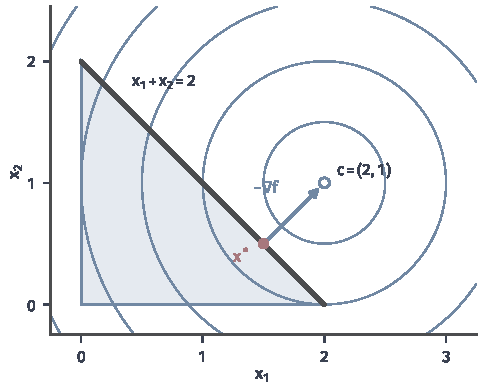
\includegraphics[width=82mm]{figures/05-optimization/06-constrained-optimization/matplotlib/kkt-budget-boundary/figure.pdf}
  \caption{预算分配（$\tau=2$）的边界最优点。浅蓝三角形是可行集，蓝色圆是目标$\frac12\lVert\bm{x}-\bm{c}\rVert_2^2$的等高线，空心点是不可行的理想分配$\bm{c}=(2,1)$，深灰粗线是起作用的预算线。红点$\bm{x}^\star=(3/2,1/2)$处，负梯度（蓝色箭头）非零，指向可行集外。}
  \label{fig:kkt-budget-boundary}
\end{BookInlineFigure}

\paragraph{一般形式}
本章和本部分后面各章都讨论下面的问题。给定$\bm{x}\in\mathbb{R}^n$的目标函数$f$、不等式约束函数$g_1,\ldots,g_m$和等式约束函数$h_1,\ldots,h_p$，求解
\begin{equation}
 \begin{aligned}
  \min_{\bm{x}\in\mathbb{R}^n}\quad&f(\bm{x})\\
  \text{s.t.}\quad&g_i(\bm{x})\leq0,\quad i=1,\ldots,m,\\
  &h_j(\bm{x})=0,\quad j=1,\ldots,p.
 \end{aligned}
 \label{eq:kkt-problem}
\end{equation}
可行集记为
\begin{equation}
 \bm{C}=\{\bm{x}\in\mathbb{R}^n:g_i(\bm{x})\leq0,\ i=1,\ldots,m;\ h_j(\bm{x})=0,\ j=1,\ldots,p\}.
 \label{eq:kkt-feasible}
\end{equation}

除非另有说明，假设$f$、$g_i$、$h_j$都定义在包含$\bm{C}$的开集上，并且连续可微；讨论二阶条件时再要求二阶连续可微。所有不等式都整理成“$\leq0$”，这个约定决定了后面乘子的符号。预算分配写成这种形式，三个不等式约束是
\begin{equation}
 g_1(\bm{x})=x_1+x_2-\tau,\qquad g_2(\bm{x})=-x_1,\qquad g_3(\bm{x})=-x_2.
 \label{eq:kkt-budget-constraints}
\end{equation}
它们的梯度依次是常向量$(1,1)$、$(-1,0)$、$(0,-1)$，都指向使约束函数增大的一侧，也就是可行集的外侧。

\paragraph{活动约束}
站在一个可行点$\bar{\bm{x}}$上，不等式约束分成两类。若$g_i(\bar{\bm{x}})=0$，这条约束正好卡在边界上，稍有不慎就会违反，称它在$\bar{\bm{x}}$处是\term{活动约束}（active constraint）。若$g_i(\bar{\bm{x}})<0$，$g_i$是连续函数，所以在$\bar{\bm{x}}$的某个邻域内仍有$g_i<0$，这条约束在局部不起任何限制作用。活动约束的下标集记为
\begin{equation}
 A(\bar{\bm{x}})=\{i\in\{1,\ldots,m\}:g_i(\bar{\bm{x}})=0\},
 \label{eq:kkt-active-set}
\end{equation}
称为\term{活动集}（active set）。等式约束总在起作用，但$A(\bar{\bm{x}})$只记不等式的下标。

图~\ref{fig:kkt-active-sets}取$\tau=2$，看三个可行点。内部点$(0.6,0.6)$没有活动约束，四周都能走。预算线上的点$(3/2,1/2)$只有$g_1$活动，能走的方向少了一半。角点$(2,0)$处$g_1$与$g_3$同时活动，能走的方向只剩一个楔形。虚线圆是一个小邻域，圆内真正影响移动的只有粗线。

\begin{BookInlineFigure}
  \centering
  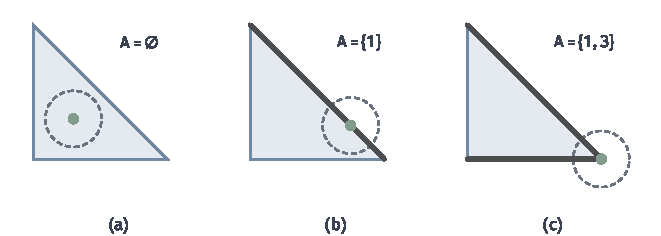
\includegraphics[width=112mm]{figures/05-optimization/06-constrained-optimization/matplotlib/kkt-active-sets/figure.pdf}
  \caption{预算三角形（$\tau=2$）中三个可行点的活动集。深灰粗线是该点的活动约束，虚线圆是一个小邻域。(a)内部点$(0.6,0.6)$没有活动约束。(b)预算线上的点$(3/2,1/2)$只有$g_1$活动。(c)角点$(2,0)$处$g_1$、$g_3$同时活动。}
  \label{fig:kkt-active-sets}
\end{BookInlineFigure}

\paragraph{局部与全局最小点}
第~\ref{chap:optimization}章区分了局部与全局最优解，本章沿用这两个概念，并按习惯称最优解为最小点。称可行点$\bm{x}^\star$是\term{局部最小点}（local minimizer），如果存在$r>0$，使
\begin{equation}
 f(\bm{x}^\star)\leq f(\bm{x})\quad\text{对所有}\ \bm{x}\in\bm{C},\ \lVert\bm{x}-\bm{x}^\star\rVert_2<r.
 \label{eq:kkt-local-min}
\end{equation}
若对$\bm{x}\neq\bm{x}^\star$不等式都严格成立，就称为严格局部最小点。要是式~\eqref{eq:kkt-local-min}对所有$\bm{x}\in\bm{C}$成立，$\bm{x}^\star$就是全局最小点。

比较只在可行点之间进行，所以邻域外和可行集外的点都不参加比较。下面的例子可以看出局部和全局的差别，而这两种点都可以落在边界上。在平面上最小化$f(\bm{x})=x_1$，约束是
\[
 g(\bm{x})=(x_2^2-1)^2+0.3\,x_2-x_1\leq0.
\]
可行集的左边界是一条弯曲的曲线，它有两个向左伸的凸起。

图~\ref{fig:kkt-local-global}中，每个凸起的顶点都比附近的可行点更靠左，因此都是局部最小点。解一元方程求边界曲线的极小，得到上方顶点约为$(0.294,0.960)$，下方顶点约为$(-0.305,-1.036)$，后者才是全局最小点。两处的梯度都等于$(1,0)$，并不为零。站在局部最小点上，只看附近无从知道下方还有更低的点，所以局部信息最多只能回答局部问题。

\begin{BookInlineFigure}
  \centering
  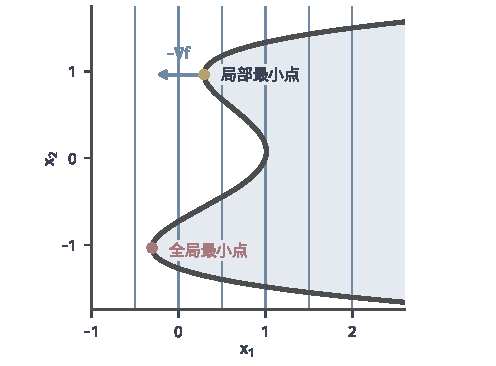
\includegraphics[width=84mm]{figures/05-optimization/06-constrained-optimization/matplotlib/kkt-local-global/figure.pdf}
  \caption{边界上的局部最小点与全局最小点。目标$f(\bm{x})=x_1$的等高线是竖直的蓝线，浅蓝区域是可行集$x_1\geq(x_2^2-1)^2+0.3x_2$，深灰粗线是边界。黄点是局部最小点，红点是全局最小点，两点的负梯度（蓝色箭头）都指向可行集外。}
  \label{fig:kkt-local-global}
\end{BookInlineFigure}

判断最优性时，本章要回答三个不同的问题：局部最小点必须满足什么（必要条件）？满足什么就一定是局部最小点（局部充分条件）？什么时候局部信息足以断定全局最优？解的存在性由第~\ref{chap:optimization}章的结论负责，例如预算三角形是非空紧集，目标连续，最优解一定存在。

\section{可行变化}
\label{sec:kkt-variations}

无约束时，最优性的论证是沿每个方向走一小步，目标都不能下降。有了约束，问题变成：站在候选点上，究竟可以朝哪些方向移动？本节先只看可行集合本身回答这个问题，再看约束函数给出的线性近似，并比较两者。这两个对象不同：前者是真实能走的方向，后者是约束函数在一阶意义下允许的方向。

\subsection{直线移动与切锥}
\label{sec:kkt-tangent-cone}

\paragraph{沿直线可行}
第~\ref{chap:optimization}章已经定义了可行方向：若$t>0$充分小时$\bar{\bm{x}}+t\bm{d}\in\bm{C}$，就称$\bm{d}$是$\bar{\bm{x}}$处的可行方向。可行集凸的时候，这个概念够用。任取$\bm{y}\in\bm{C}$，线段$\bar{\bm{x}}+t(\bm{y}-\bar{\bm{x}})$（$0\leq t\leq1$）都在$\bm{C}$里，所以每个$\bm{y}-\bar{\bm{x}}$都是可行方向，如图~\ref{fig:kkt-line-vs-arc}(a)。

\begin{BookInlineFigure}
  \centering
  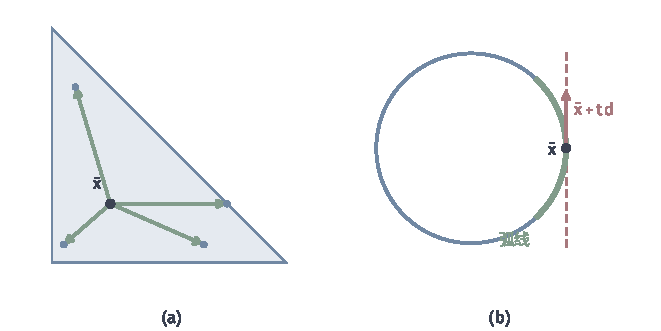
\includegraphics[width=112mm]{figures/05-optimization/06-constrained-optimization/matplotlib/kkt-line-vs-arc/figure.pdf}
  \caption{直线移动与弧线移动。(a)凸集中，从$\bar{\bm{x}}$到任意可行点的线段（绿色箭头）都留在集合内。(b)可行集是单位圆周（蓝线）。从$\bar{\bm{x}}=(1,0)$沿切线走的红色直线立刻离开圆周，而绿色弧线一直可行，并且在$\bar{\bm{x}}$处与直线相切。}
  \label{fig:kkt-line-vs-arc}
\end{BookInlineFigure}

可行集弯曲时，这个定义就不够用了。设$\bm{C}$是单位圆周，也就是$h(\bm{x})=x_1^2+x_2^2-1=0$的解集，取$\bar{\bm{x}}=(1,0)$。若$\bar{\bm{x}}+t\bm{d}$对小的$t>0$都在圆周上，展开$h$并除以$t$，得到
\[
 2d_1+t\lVert\bm{d}\rVert_2^2=0\quad\text{对所有充分小的}\ t>0.
\]
令$t$取两个不同的值，两式相减得$\lVert\bm{d}\rVert_2=0$。所以除零方向外没有可行方向。

可是点明明能沿圆周移动，图~\ref{fig:kkt-line-vs-arc}(b)的绿色弧线就是这样的移动。直线走不通，弧线走得通，弧线在出发时的速度方向是$(0,1)$。因此“能走的方向”不应理解成沿直线可行，而应理解成沿某条可行路径出发的速度。

\paragraph{用放大镜定义方向}
为了把这个想法写成定义，可以想象拿放大镜对准$\bar{\bm{x}}$看可行集。放大倍数越高，圆弧看起来越直，极限是一条直线。写成算式，就是取趋于$\bar{\bm{x}}$的可行点列，把位移除以一个趋于零的正数，看它的极限。

\begin{definition}[切锥]
\label{def:kkt-tangent-cone}
设$\bm{C}\subseteq\mathbb{R}^n$，$\bar{\bm{x}}\in\bm{C}$。称$\bm{d}\in\mathbb{R}^n$是$\bm{C}$在$\bar{\bm{x}}$处的切向量，如果存在可行点列$\bm{x}^{(k)}\in\bm{C}$与正数列$t_k$，使$\bm{x}^{(k)}\to\bar{\bm{x}}$，$t_k\downarrow0$，并且
\begin{equation}
 \frac{\bm{x}^{(k)}-\bar{\bm{x}}}{t_k}\to\bm{d}.
 \label{eq:kkt-tangent-limit}
\end{equation}
全体切向量组成的集合称为\term{切锥}（tangent cone），记为$\bm{T}_{\bm{C}}(\bar{\bm{x}})$。
\end{definition}

上标$(k)$是点列编号，不表示算法迭代。这里$1/t_k$就是放大倍数，点列可以是沿曲线取的点，也可以是在集合中跳跃着逼近的点。沿固定直线可行的方向一定是切向量：取$\bm{x}^{(k)}=\bar{\bm{x}}+t_k\bm{d}$即可。反过来不成立，圆周就是反例。

下面在圆周上走一遍定义。取$t_k=2^{-(k-1)}$，$\bm{x}^{(k)}=(\cos t_k,\sin t_k)$，放大后的位移是
\[
 \frac{\bm{x}^{(k)}-\bar{\bm{x}}}{t_k}=\Bigl(\frac{\cos t_k-1}{t_k},\frac{\sin t_k}{t_k}\Bigr).
\]
前三项依次约为$(-0.460,0.841)$、$(-0.245,0.959)$、$(-0.124,0.990)$，极限是$(0,1)$。

图~\ref{fig:kkt-tangent-sequence}左边是原始尺度下的割线，它们越来越贴近圆弧；右边是放大后的位移，绿色箭头收拢到红色的$(0,1)$。换成$t_k/s$（$s>0$）作分母，极限变成$s(0,1)$；沿圆周的另一侧取点，得到$-s(0,1)$。所以切锥至少包含整条竖直直线。下一小节会用约束函数证明切锥恰好就是这条直线。

\begin{BookInlineFigure}
  \centering
  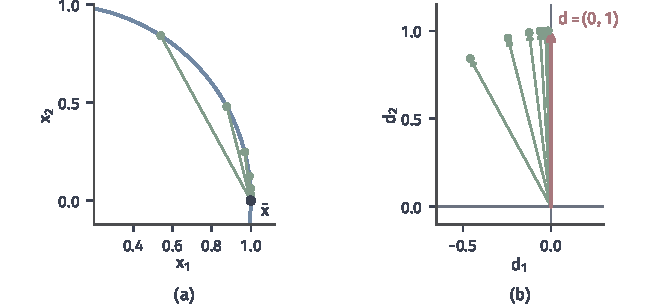
\includegraphics[width=112mm]{figures/05-optimization/06-constrained-optimization/matplotlib/kkt-tangent-sequence/figure.pdf}
  \caption{切向量是放大后位移的极限。可行集为单位圆周，$\bar{\bm{x}}=(1,0)$，$t_k=2^{-(k-1)}$（$k=1,\ldots,6$）。(a)绿点是$\bm{x}^{(k)}=(\cos t_k,\sin t_k)$，绿线是割线。(b)绿色箭头是$(\bm{x}^{(k)}-\bar{\bm{x}})/t_k$，它们趋于红色箭头$\bm{d}=(0,1)$。}
  \label{fig:kkt-tangent-sequence}
\end{BookInlineFigure}

\paragraph{切锥的基本性质}
后面的证明要用到切锥的两条性质，第二条尤其重要，它允许我们用切向量的极限产生新的切向量。

\begin{lemma}[切锥是闭锥]
\label{lem:kkt-tangent-closed}
$\bm{T}_{\bm{C}}(\bar{\bm{x}})$包含零向量，对正数倍封闭，并且是闭集。
\end{lemma}

\begin{proof}
取$\bm{x}^{(k)}=\bar{\bm{x}}$就得到零向量。若$\bm{d}$对应$(\bm{x}^{(k)},t_k)$，$s>0$，则同一点列配$t_k/s$给出$s\bm{d}$。

再证闭性。设切向量列$\bm{d}_l\to\bm{d}$。对每个$l$，由定义可以在$\bm{d}_l$对应的点列中取一项，得到可行点$\bm{y}_l$和正数$\epsilon_l<1/l$，使
\[
 \lVert\bm{y}_l-\bar{\bm{x}}\rVert_2\leq\frac1l,\qquad
 \Bigl\lVert\frac{\bm{y}_l-\bar{\bm{x}}}{\epsilon_l}-\bm{d}_l\Bigr\rVert_2\leq\frac1l.
\]
令$l\to\infty$，有$\bm{y}_l\to\bar{\bm{x}}$，$\epsilon_l\to0$（必要时取子列使$\epsilon_l$单调递减），位移比趋于$\bm{d}$。所以$\bm{d}$是切向量。
\end{proof}

图~\ref{fig:kkt-tangent-cones}是几种常见的形状。内点处四周都能走，切锥是全空间。光滑边界上，放大后边界变成直线，切锥是半空间。角点处切锥是楔形。尖点处两条边界相切，放大后楔形被压成一条线，切锥只剩一条射线。

\begin{BookInlineFigure}
  \centering
  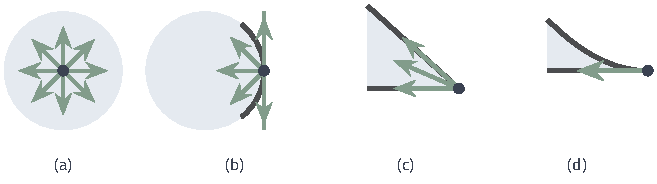
\includegraphics[width=111.3mm]{figures/05-optimization/06-constrained-optimization/tikz/kkt-tangent-cones/figure.pdf}
  \caption{切锥的四种形状。浅蓝区域是可行集，黑点是基点，绿色箭头表示切向量，深灰粗线是边界。(a)内点：全部方向。(b)光滑边界：半空间，边界上的绿线是它的分界。(c)角点：楔形。(d)尖点：只有一条射线。}
  \label{fig:kkt-tangent-cones}
\end{BookInlineFigure}

切锥未必是凸集。集合$\{\bm{x}:x_1x_2=0\}$由两条坐标轴组成，它在原点的切锥就是这两条坐标轴本身。名字里的“锥”只表示对正数倍封闭。

\subsection{一阶必要条件}
\label{sec:kkt-first-order}

现在可以回答：局部最小点在切向量上要满足什么？直观上，沿任何可行路径出发，目标都不能以一阶速度下降。把路径换成切锥定义中的点列，证明只需要一次Taylor展开。

\begin{theorem}[切锥上的一阶必要条件]
\label{thm:kkt-tangent-necessary}
设$\bm{x}^\star$是$f$在$\bm{C}$上的局部最小点，$f$在$\bm{x}^\star$处可微。则
\begin{equation}
 \langle\nabla f(\bm{x}^\star),\bm{d}\rangle\geq0\quad\text{对所有}\ \bm{d}\in\bm{T}_{\bm{C}}(\bm{x}^\star).
 \label{eq:kkt-tangent-necessary}
\end{equation}
\end{theorem}

\begin{proof}
取切向量$\bm{d}$及相应的$\bm{x}^{(k)}$、$t_k$，记位移$\bm{u}_k=\bm{x}^{(k)}-\bm{x}^\star$。$f$在$\bm{x}^\star$处可微，所以
\[
 f(\bm{x}^{(k)})-f(\bm{x}^\star)=\langle\nabla f(\bm{x}^\star),\bm{u}_k\rangle+r_k,
 \qquad\frac{r_k}{\lVert\bm{u}_k\rVert_2}\to0,
\]
其中$\bm{u}_k=\bm{0}$时取$r_k=0$，比值按零理解。

$k$充分大时$\bm{x}^{(k)}$落在式~\eqref{eq:kkt-local-min}的邻域内，左端非负。两边除以$t_k$，得到
\[
 0\leq\Bigl\langle\nabla f(\bm{x}^\star),\frac{\bm{u}_k}{t_k}\Bigr\rangle+\frac{r_k}{t_k}.
\]

由$\bm{u}_k/t_k\to\bm{d}$知$\lVert\bm{u}_k\rVert_2/t_k$有界，所以$r_k/t_k\to0$。令$k\to\infty$，即得式~\eqref{eq:kkt-tangent-necessary}。
\end{proof}

在预算例上试用这个条件（$\tau=2$）。先看不是最优的点$\bar{\bm{x}}=(1,1)$，它在预算线上，梯度是$(-1,0)$。沿预算线的切向量$\bm{d}=(1,-1)$有
\[
 \langle\nabla f(\bar{\bm{x}}),\bm{d}\rangle=-1<0.
\]
直接代入也一样：$f(1+s,1-s)=\frac12[(1-s)^2+s^2]$在$s=0$处的导数是$-1$。所以$(1,1)$不是局部最小点。

再看$\bm{x}^\star=(3/2,1/2)$。这里切锥是半平面$\{\bm{d}:d_1+d_2\leq0\}$，梯度是$(-1/2,-1/2)$，于是对切锥中每个$\bm{d}$，
\[
 \langle\nabla f(\bm{x}^\star),\bm{d}\rangle=-\frac12(d_1+d_2)\geq0.
\]
必要条件成立。图~\ref{fig:kkt-first-order-test}比较了这两个点：(a)中负梯度有沿边界的分量，绿色切向量与负梯度成锐角；(b)中负梯度与边界垂直，沿边界两侧移动都没有一阶下降。

\begin{BookInlineFigure}
  \centering
  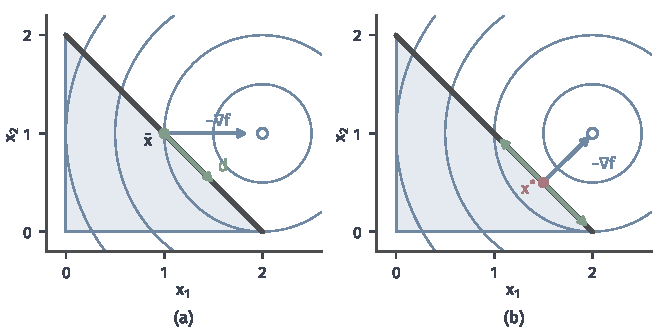
\includegraphics[width=112mm]{figures/05-optimization/06-constrained-optimization/matplotlib/kkt-first-order-test/figure.pdf}
  \caption{切向量上的一阶检验（预算例，$\tau=2$）。空心点是理想分配$\bm{c}$，蓝色箭头是负梯度，绿色箭头是沿预算线的切向量。(a)在$\bar{\bm{x}}=(1,1)$，切向量$\bm{d}=(1,-1)$与负梯度成锐角，目标可以下降。(b)在红点$\bm{x}^\star=(3/2,1/2)$，负梯度垂直于预算线，不存在下降的切向量。}
  \label{fig:kkt-first-order-test}
\end{BookInlineFigure}

\paragraph{凸可行集：法锥}
可行集凸时，每个$\bm{y}-\bm{x}^\star$都是切向量，所以条件可以写成对全部可行点的检验，把切向量这个中间概念拿掉。我们把这个条件从“梯度与所有可行方向的夹角”改写到集合一侧，定义所有“指向集合外”的向量。

\begin{definition}[法锥]
\label{def:kkt-normal-cone}
设$\bm{C}\subseteq\mathbb{R}^n$是凸集，$\bar{\bm{x}}\in\bm{C}$。集合
\begin{equation}
 \bm{N}_{\bm{C}}(\bar{\bm{x}})=\{\bm{v}\in\mathbb{R}^n:\langle\bm{v},\bm{y}-\bar{\bm{x}}\rangle\leq0\ \text{对所有}\ \bm{y}\in\bm{C}\}
 \label{eq:kkt-normal-cone}
\end{equation}
称为$\bm{C}$在$\bar{\bm{x}}$处的\term{法锥}（normal cone）。
\end{definition}

法锥里的向量与所有从$\bar{\bm{x}}$出发的可行弦成钝角或直角，它们都指向集合外侧。负梯度只要落在法锥里，朝可行集内部就没有一阶下降。

\begin{theorem}[凸可行集上的一阶条件]
\label{thm:kkt-convex-set-first-order}
设$\bm{C}$是凸集，$f$在包含$\bm{C}$的开集上可微，$\bm{x}^\star\in\bm{C}$。若$\bm{x}^\star$是$f$在$\bm{C}$上的局部最小点，则
\begin{equation}
 \langle\nabla f(\bm{x}^\star),\bm{y}-\bm{x}^\star\rangle\geq0\quad\text{对所有}\ \bm{y}\in\bm{C},
 \label{eq:kkt-vi}
\end{equation}
等价地，$-\nabla f(\bm{x}^\star)\in\bm{N}_{\bm{C}}(\bm{x}^\star)$。若$f$还在$\bm{C}$上凸，则式~\eqref{eq:kkt-vi}也推出$\bm{x}^\star$是全局最小点。
\end{theorem}

\begin{proof}
必要性：$\bm{y}-\bm{x}^\star$是可行方向，也是切向量，由定理~\ref{thm:kkt-tangent-necessary}得到式~\eqref{eq:kkt-vi}。等价写法只是把$\bm{v}=-\nabla f(\bm{x}^\star)$代入式~\eqref{eq:kkt-normal-cone}。

充分性：取$\bm{y}\in\bm{C}$，$t\in(0,1]$。由$f$的凸性，
\[
 f\bigl(\bm{x}^\star+t(\bm{y}-\bm{x}^\star)\bigr)\leq(1-t)f(\bm{x}^\star)+tf(\bm{y}).
\]
移项，除以$t$，再令$t\downarrow0$，左端的差商趋于方向导数，于是
\[
 \langle\nabla f(\bm{x}^\star),\bm{y}-\bm{x}^\star\rangle\leq f(\bm{y})-f(\bm{x}^\star).
\]
由式~\eqref{eq:kkt-vi}，左端非负，所以$f(\bm{y})\geq f(\bm{x}^\star)$。
\end{proof}

式~\eqref{eq:kkt-vi}称为\term{变分不等式}（variational inequality）。图~\ref{fig:kkt-normal-cones}让预算$\tau$从大变小，法锥依次是三种形状。

$\tau=4$时最优点$\bm{c}=(2,1)$在内部，法锥只有零向量，条件退化为$\nabla f=\bm{0}$。$\tau=2$时最优点在预算线上，法锥是外法向$(1,1)$方向的射线，$-\nabla f=(1/2,1/2)$落在上面。

$\tau=1/2$时，最优点是角点$(1/2,0)$。法锥由两条边的外法向$(1,1)$、$(0,-1)$张成。这一点可以直接核对：设$\bm{v}\in\bm{N}_{\bm{C}}$，用沿两条边的可行弦方向$(-1,1)$与$(-1,0)$代入式~\eqref{eq:kkt-normal-cone}，得到$v_2\leq v_1$与$v_1\geq0$，这恰好说明
\[
 \bm{v}=v_1(1,1)+(v_1-v_2)(0,-1),\qquad v_1\geq0,\ v_1-v_2\geq0.
\]
角点的法锥比边上的法锥大，能接住更多方向的负梯度。

\begin{BookInlineFigure}
  \centering
  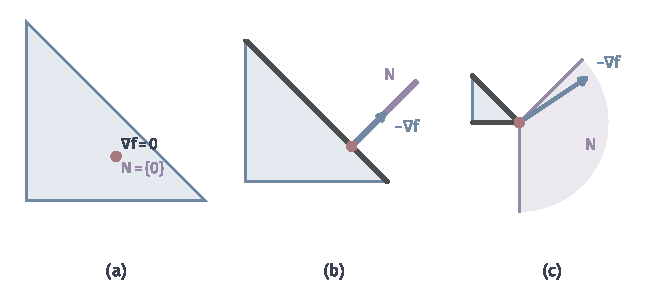
\includegraphics[width=112mm]{figures/05-optimization/06-constrained-optimization/matplotlib/kkt-normal-cones/figure.pdf}
  \caption{预算例中最优点处的法锥（紫色）。红点是最优点，蓝色箭头是负梯度（(c)中按$0.5$倍缩短）。(a)$\tau=4$，最优点在内部，法锥为$\{\bm{0}\}$。(b)$\tau=2$，法锥是一条射线，负梯度落在上面。(c)$\tau=1/2$，最优点是角点，法锥是两条外法向张成的楔形，负梯度落在其中。}
  \label{fig:kkt-normal-cones}
\end{BookInlineFigure}

定理的充分性同时需要可行集与目标都凸。只有目标凸是不够的：在单位圆周上最小化$\frac12\lVert\bm{x}-(2,0)\rVert_2^2$，点$(-1,0)$的梯度是$(-3,0)$，切向量只有$(0,s)$，与梯度垂直，一阶条件成立；可它是圆周上离$(2,0)$最远的点。本章后面还会回到这个例子。

\subsection{约束的线性化}
\label{sec:kkt-linearized}

切锥描述得准，却不好算，我们无法枚举所有点列。约束以函数形式给出时，有一个自然的替代品：在基点把约束函数展开到一阶，看一阶近似允许哪些方向。

设$\bar{\bm{x}}$可行，沿$\bm{d}$走一小步，约束函数近似变化为
\[
 g_i(\bar{\bm{x}}+t\bm{d})\approx g_i(\bar{\bm{x}})+t\langle\nabla g_i(\bar{\bm{x}}),\bm{d}\rangle.
\]
不活动的约束有余量，一阶近似不构成限制。活动约束要求这一项不为正，等式约束要求它等于零。

\begin{definition}[线性化锥]
\label{def:kkt-linearized-cone}
设$\bar{\bm{x}}\in\bm{C}$，约束函数在$\bar{\bm{x}}$处可微。集合
\begin{equation}
 \bm{F}(\bar{\bm{x}})=\left\{\bm{d}\in\mathbb{R}^n:
 \begin{aligned}
  &\langle\nabla h_j(\bar{\bm{x}}),\bm{d}\rangle=0,\ j=1,\ldots,p,\\
  &\langle\nabla g_i(\bar{\bm{x}}),\bm{d}\rangle\leq0,\ i\in A(\bar{\bm{x}})
 \end{aligned}
 \right\}
 \label{eq:kkt-linearized-cone}
\end{equation}
称为$\bar{\bm{x}}$处的\term{线性化锥}（linearized cone）。
\end{definition}

$\bm{F}(\bar{\bm{x}})$是有限个线性不等式的解集，一眼就能写出。例如预算例$\tau=1/2$的角点$(1/2,0)$处，$g_1$和$g_3$活动，于是
\[
 \bm{F}=\{\bm{d}:d_1+d_2\leq0,\ -d_2\leq0\}.
\]
单位圆周在$(1,0)$处，$\nabla h=(2,0)$，于是$\bm{F}=\{\bm{d}:d_1=0\}$，正是前面算出的竖直直线。

真实能走的方向一定通过这个一阶检查，因此切锥总在线性化锥之内。

\begin{theorem}[切锥包含于线性化锥]
\label{thm:kkt-tangent-in-linearized}
设$\bar{\bm{x}}\in\bm{C}$，$g_i$（$i\in A(\bar{\bm{x}})$）与$h_j$在$\bar{\bm{x}}$处可微。则
\begin{equation}
 \bm{T}_{\bm{C}}(\bar{\bm{x}})\subseteq\bm{F}(\bar{\bm{x}}).
 \label{eq:kkt-tangent-in-linearized}
\end{equation}
\end{theorem}

\begin{proof}
取切向量$\bm{d}$及相应的$\bm{x}^{(k)}$、$t_k$，对活动的$g_i$，由可微性，
\[
 g_i(\bm{x}^{(k)})=g_i(\bar{\bm{x}})+\langle\nabla g_i(\bar{\bm{x}}),\bm{x}^{(k)}-\bar{\bm{x}}\rangle+o(\lVert\bm{x}^{(k)}-\bar{\bm{x}}\rVert_2).
\]
这里$g_i(\bar{\bm{x}})=0$，$g_i(\bm{x}^{(k)})\leq0$。除以$t_k$并令$k\to\infty$，余项如定理~\ref{thm:kkt-tangent-necessary}的证明一样趋于零，得到
\[
 \langle\nabla g_i(\bar{\bm{x}}),\bm{d}\rangle\leq0.
\]

对$h_j$同样展开，此时左端恒为零，极限给出$\langle\nabla h_j(\bar{\bm{x}}),\bm{d}\rangle=0$。
\end{proof}

圆周的例子到这里算完了：切锥包含竖直直线，又包含于$\bm{F}=\{\bm{d}:d_1=0\}$，所以它就是这条直线。

式~\eqref{eq:kkt-tangent-in-linearized}可以是严格包含。考虑一维约束$g(x)=x^2\leq0$，可行集只有原点，切锥是$\{0\}$。可是$g'(0)=0$，线性化没有施加任何限制，$\bm{F}(0)=\mathbb{R}$。一阶近似把这条弯曲的约束看成了常值零，图~\ref{fig:kkt-linearization}(b)的黄色线就是这个近似。

\begin{BookInlineFigure}
  \centering
  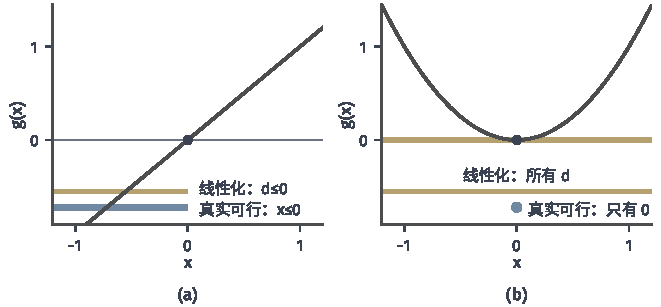
\includegraphics[width=112mm]{figures/05-optimization/06-constrained-optimization/matplotlib/kkt-linearization/figure.pdf}
  \caption{线性化与真实可行集的比较。深灰曲线是$g$，下方黄带是线性化允许的方向，蓝带（点）是真实的可行点。(a)$g(x)=x$，线性化与真实情况一致。(b)$g(x)=x^2$，$g'(0)=0$，切线（黄色）恒为零，线性化允许所有方向，而可行集只有原点。}
  \label{fig:kkt-linearization}
\end{BookInlineFigure}

二维的例子能看得更清楚。取$g_1(\bm{x})=x_2-(1-x_1)^3\leq0$，$g_2(\bm{x})=-x_2\leq0$，点$\bar{\bm{x}}=(1,0)$，两条约束都活动。可行点要满足$0\leq x_2\leq(1-x_1)^3$，所以$x_1\leq1$，可行集在$\bar{\bm{x}}$处形成一个向右的尖点。

梯度分别是$(0,1)$和$(0,-1)$，线性化要求$d_2\leq0$且$-d_2\leq0$，即$d_2=0$，于是
\[
 \bm{F}(\bar{\bm{x}})=\{\bm{d}:d_2=0\},\qquad
 \bm{T}_{\bm{C}}(\bar{\bm{x}})=\{(-s,0):s\geq0\}.
\]
线性化多出了向右的半条直线。图~\ref{fig:kkt-cusp}中的红色箭头就是虚假方向：若最小化$f(\bm{x})=-x_1$，$\bar{\bm{x}}$是全局最小点，而$\bm{d}=(1,0)$在线性化下“可行”，并使$\langle\nabla f,\bm{d}\rangle=-1<0$。只看线性化，就会误以为还能下降。

\begin{BookInlineFigure}
  \centering
  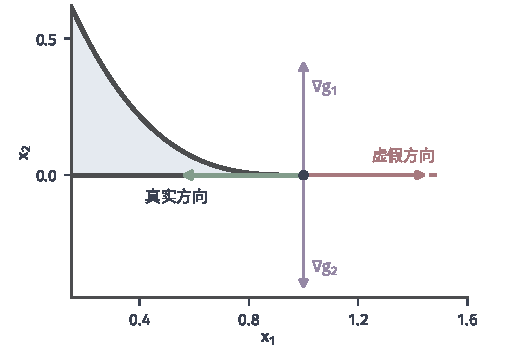
\includegraphics[width=88mm]{figures/05-optimization/06-constrained-optimization/matplotlib/kkt-cusp/figure.pdf}
  \caption{尖点处线性化引入虚假方向。浅蓝区域是可行集$0\leq x_2\leq(1-x_1)^3$，紫色箭头是两条活动约束的梯度$(0,\pm1)$。线性化只要求$d_2=0$，向左的绿色箭头是真实切向量，向右的红色箭头是虚假方向。}
  \label{fig:kkt-cusp}
\end{BookInlineFigure}

表~\ref{tab:kkt-tangent-vs-linearized}对比这两个对象。下一节要回答的问题由此而来：什么时候两者相等，使我们可以用好算的线性化锥代替真实的切锥？

\begin{BookInlineTable}
  \centering
  \begin{tabular}{@{}lll@{}}
    \toprule
    对比项 & 切锥$\bm{T}_{\bm{C}}$ & 线性化锥$\bm{F}$\\
    \midrule
    依赖什么 & 只依赖集合$\bm{C}$ & 依赖约束函数的写法\\
    含义 & 真实可行变化 & 一阶模型允许的变化\\
    计算 & 一般需要分析点列 & 解线性不等式\\
    关系 & 总包含在$\bm{F}$内 & 可能多出虚假方向\\
    \bottomrule
  \end{tabular}
  \caption{切锥与线性化锥的比较。}
  \label{tab:kkt-tangent-vs-linearized}
\end{BookInlineTable}

\section{约束资格}
\label{sec:kkt-cq}

定理~\ref{thm:kkt-tangent-necessary}是关于切锥的，而能算的是线性化锥。两者之间差一个包含关系。本节研究：约束函数在一点满足什么条件，线性化就没有引入虚假方向，也就是切锥等于线性化锥？这类只涉及约束函数、不涉及目标的条件称为\term{约束资格}（constraint qualification）。

约束资格和凸性是两回事。约束$x^2\leq0$是凸函数，问题也可以是凸的，但它的线性化在原点失效。反过来，圆周这样的非凸集合，线性化却是准确的。约束资格检查的是约束函数在这一点的一阶信息够不够用，和目标函数是否凸没有关系。

\subsection{线性无关约束资格}
\label{sec:kkt-licq}

先看线性化为什么可能准确。在圆周的$(1,0)$处，沿切线走一步$(1,t)$会离开圆周，但偏离只有$t$的二阶小量，沿圆的法向拉回去一点，就回到圆周上。拉回动作所需的修正量比$t$小得多，放大看不出来，所以切线方向是真实可行的。

这个拉回动作要能实施，需要约束的梯度在拉回的方向上足够“有劲”，也就是各约束可以被独立地修正。这就是下面的条件。

\begin{definition}[线性无关约束资格]
\label{def:kkt-licq}
设$\bar{\bm{x}}\in\bm{C}$。若向量组
\begin{equation}
 \{\nabla h_j(\bar{\bm{x}}):j=1,\ldots,p\}\cup\{\nabla g_i(\bar{\bm{x}}):i\in A(\bar{\bm{x}})\}
 \label{eq:kkt-licq}
\end{equation}
线性无关，就称$\bar{\bm{x}}$满足\term{线性无关约束资格}（linear independence constraint qualification，LICQ）。
\end{definition}

图~\ref{fig:kkt-licq-representation}(a)是预算例的角点，梯度$(1,1)$和$(0,-1)$线性无关，LICQ成立。图(c)是上一节的尖点，两个活动梯度共线，LICQ不成立。圆周上$\nabla h=(2x_1,2x_2)$处处非零，单个非零向量线性无关，LICQ处处成立。约束$x^2\leq0$在原点的梯度为零，LICQ不成立。

\begin{BookInlineFigure}
  \centering
  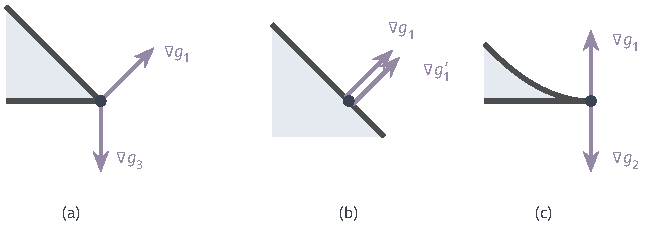
\includegraphics[width=110.3mm]{figures/05-optimization/06-constrained-optimization/tikz/kkt-licq-representation/figure.pdf}
  \caption{活动约束的梯度是否线性无关（紫色箭头）。(a)角点处两条梯度线性无关，LICQ成立。(b)同一条约束写两次，可行集不变，但两个梯度相同（为看清而错开绘制），LICQ不成立。(c)尖点处两个梯度方向相反，LICQ不成立。}
  \label{fig:kkt-licq-representation}
\end{BookInlineFigure}

下面的引理把“拉回”写成隐函数定理的一次应用，它产生一条真正可行的曲线。第~\ref{sec:kkt-second-order}节的二阶必要条件还要用这条曲线。隐函数定理说：方程关于待解变量的Jacobian可逆时，方程在局部确定唯一的连续可微解，详见\BookChapterRef{chap:implicit-inverse-functions}{卷二第22章“隐函数与反函数”}。

\begin{lemma}[沿线性化方向的可行曲线]
\label{lem:kkt-feasible-curve}
设约束函数在$\bar{\bm{x}}\in\bm{C}$附近连续可微，$\bm{d}\in\bm{F}(\bar{\bm{x}})$。设$W\subseteq A(\bar{\bm{x}})$满足：$i\in W$时$\langle\nabla g_i(\bar{\bm{x}}),\bm{d}\rangle=0$，$i\in A(\bar{\bm{x}})\setminus W$时$\langle\nabla g_i(\bar{\bm{x}}),\bm{d}\rangle<0$，并且$\nabla h_j(\bar{\bm{x}})$（全部$j$）与$\nabla g_i(\bar{\bm{x}})$（$i\in W$）线性无关。则存在$\delta>0$和连续可微曲线$\bm{x}:(-\delta,\delta)\to\mathbb{R}^n$，满足
\begin{equation}
 \bm{x}(0)=\bar{\bm{x}},\qquad\bm{x}'(0)=\bm{d},\qquad\bm{x}(t)\in\bm{C}\ \ (0\leq t<\delta),
 \label{eq:kkt-feasible-curve}
\end{equation}
并且$h_j(\bm{x}(t))=0$，$g_i(\bm{x}(t))=0$（$i\in W$）对$\lvert t\rvert<\delta$成立。若约束函数还二阶连续可微，则曲线也二阶连续可微。
\end{lemma}

\begin{proof}
把$h_j$（全部$j$）和$g_i$（$i\in W$）合成向量值函数$\bm{c}$，记它在$\bar{\bm{x}}$处的Jacobian为$\bm{J}\in\mathbb{R}^{r\times n}$。由假设，$\bm{J}$行满秩，$\bm{J}\bm{d}=\bm{0}$。考虑关于$\bm{w}\in\mathbb{R}^r$的方程
\[
 \Phi(t,\bm{w})=\bm{c}(\bar{\bm{x}}+t\bm{d}+\bm{J}^\top\bm{w})=\bm{0}.
\]
这里$\bar{\bm{x}}+t\bm{d}$是沿切线走，$\bm{J}^\top\bm{w}$是沿约束法向的修正。

$\Phi(0,\bm{0})=\bm{0}$，关于$\bm{w}$的Jacobian在该点是$\bm{J}\bm{J}^\top$，行满秩保证它可逆。由隐函数定理，存在连续可微的$\bm{w}(t)$（$\lvert t\rvert<\delta$），$\bm{w}(0)=\bm{0}$，$\Phi(t,\bm{w}(t))=\bm{0}$。隐函数的导数公式给出
\[
 \bm{w}'(0)=-(\bm{J}\bm{J}^\top)^{-1}\bm{J}\bm{d}=\bm{0}.
\]

令
\[
 \bm{x}(t)=\bar{\bm{x}}+t\bm{d}+\bm{J}^\top\bm{w}(t),
\]
于是$\bm{x}'(0)=\bm{d}$，且$\bm{c}(\bm{x}(t))=\bm{0}$。剩下的约束分两类检查。对$i\in A(\bar{\bm{x}})\setminus W$，有
\[
 g_i(\bm{x}(t))=t\langle\nabla g_i(\bar{\bm{x}}),\bm{d}\rangle+o(t),
\]
小的$t>0$时为负。对$i\notin A(\bar{\bm{x}})$，$g_i(\bar{\bm{x}})<0$，由连续性在小$t$时仍为负。缩小$\delta$后，$\bm{x}(t)$在$0\leq t<\delta$时可行。

约束函数二阶连续可微时，隐函数的导数公式
\[
 \bm{w}'(t)=-\bigl[\bm{D}_{\bm{w}}\Phi(t,\bm{w}(t))\bigr]^{-1}\bm{D}_t\Phi(t,\bm{w}(t))
\]
的右端沿解连续可微，所以$\bm{w}$二阶连续可微，曲线也是。
\end{proof}

圆周上可以把这个构造完全算出来。$\bar{\bm{x}}=(1,0)$，$\bm{d}=(0,1)$，$\bm{J}=(2,0)$，修正方程是
\[
 (1+2w)^2+t^2=1.
\]
取$w(0)=0$的解支，得到
\[
 w(t)=\frac{\sqrt{1-t^2}-1}{2}=-\frac{t^2}{4}+o(t^2),\qquad\bm{x}(t)=\bigl(\sqrt{1-t^2},\,t\bigr).
\]
修正量$w$是$t$的二阶小量，这正是$w'(0)=0$的含义。图~\ref{fig:kkt-licq-correction}画出$t=0.3,0.55,0.8$时的切线步和修正，修正量随$t$减小而更快地消失。

\begin{BookInlineFigure}
  \centering
  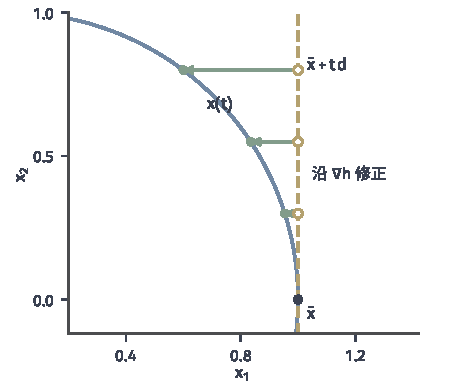
\includegraphics[width=78mm]{figures/05-optimization/06-constrained-optimization/matplotlib/kkt-licq-correction/figure.pdf}
  \caption{用隐函数定理修正线性化方向。蓝线是单位圆周，黄色虚线是切线$\bar{\bm{x}}+t\bm{d}$，黄色空心点是不可行的试探点。绿色箭头沿$\nabla h(\bar{\bm{x}})$方向把试探点拉回圆周，绿点组成可行曲线$\bm{x}(t)$。$t$越小，修正量相对$t$越小。}
  \label{fig:kkt-licq-correction}
\end{BookInlineFigure}

有了可行曲线，线性化方向就全部是真实方向。

\begin{theorem}[LICQ下线性化准确]
\label{thm:kkt-licq-exact}
设约束函数在$\bar{\bm{x}}\in\bm{C}$附近连续可微，$\bar{\bm{x}}$满足LICQ。则
\begin{equation}
 \bm{T}_{\bm{C}}(\bar{\bm{x}})=\bm{F}(\bar{\bm{x}}).
 \label{eq:kkt-licq-exact}
\end{equation}
\end{theorem}

\begin{proof}
包含$\subseteq$是定理~\ref{thm:kkt-tangent-in-linearized}。反过来取$\bm{d}\in\bm{F}(\bar{\bm{x}})$，令
\[
 W=\{i\in A(\bar{\bm{x}}):\langle\nabla g_i(\bar{\bm{x}}),\bm{d}\rangle=0\}.
\]
LICQ保证引理~\ref{lem:kkt-feasible-curve}的线性无关假设成立，得到可行曲线。取$t_k=\delta/(k+1)$，$\bm{x}^{(k)}=\bm{x}(t_k)$，由$\bm{x}'(0)=\bm{d}$知式~\eqref{eq:kkt-tangent-limit}成立，所以$\bm{d}$是切向量。
\end{proof}

\paragraph{条件与约束的写法有关}
LICQ是对约束函数的要求，不是对集合的要求。把预算约束$x_1+x_2\leq\tau$写两遍，可行集一点没变，切锥也没变，但活动梯度$(1,1)$出现两次，线性相关，LICQ就不成立了，见图~\ref{fig:kkt-licq-representation}(b)。这说明LICQ可以因为写法上的冗余而失败，并不代表集合本身有什么毛病。下一小节的条件能容忍这种冗余。

\subsection{Mangasarian--Fromovitz条件}
\label{sec:kkt-mfcq}

回头看证明，线性化准确真正需要什么？对活动不等式来说，严格向内的方向不必拉回，因为它们本来就有一阶余量。只有等式约束要靠拉回来保持。所以只需要等式约束可以被独立修正，并且存在一个同时严格改善所有活动不等式的方向。

\begin{definition}[Mangasarian--Fromovitz约束资格]
\label{def:kkt-mfcq}
设$\bar{\bm{x}}\in\bm{C}$。若$\nabla h_j(\bar{\bm{x}})$（$j=1,\ldots,p$）线性无关，并且存在$\bar{\bm{d}}\in\mathbb{R}^n$，使
\begin{equation}
 \begin{aligned}
  \langle\nabla h_j(\bar{\bm{x}}),\bar{\bm{d}}\rangle&=0,\quad j=1,\ldots,p,\\
  \langle\nabla g_i(\bar{\bm{x}}),\bar{\bm{d}}\rangle&<0,\quad i\in A(\bar{\bm{x}}),
 \end{aligned}
 \label{eq:kkt-mfcq}
\end{equation}
就称$\bar{\bm{x}}$满足\term{Mangasarian--Fromovitz约束资格}（Mangasarian--Fromovitz constraint qualification，MFCQ）。
\end{definition}

条件的两部分各有用途：等式梯度线性无关让我们能用隐函数定理保持等式；方向$\bar{\bm{d}}$让我们能严格走进不等式的内部。图~\ref{fig:kkt-mfcq-direction}(a)中三条活动梯度在平面内必然线性相关，LICQ不成立，但它们都落在某个开半平面内，绿色的$\bar{\bm{d}}$同时与三者成钝角，MFCQ成立。图(b)是尖点：要求$\bar{d}_2<0$与$-\bar{d}_2<0$，两个开半平面不相交，这样的方向不存在。

\begin{BookInlineFigure}
  \centering
  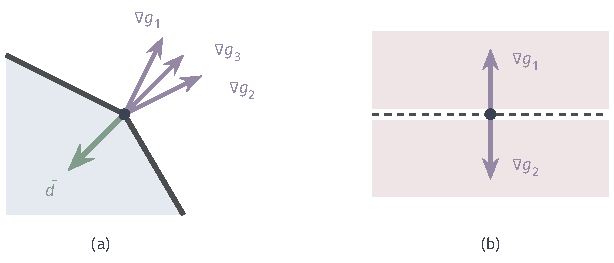
\includegraphics[width=103.9mm]{figures/05-optimization/06-constrained-optimization/tikz/kkt-mfcq-direction/figure.pdf}
  \caption{MFCQ要求存在严格向内的方向。(a)三条活动约束的梯度（紫色）线性相关，但绿色方向$\bar{\bm{d}}$与三者都成钝角，MFCQ成立。(b)两个活动梯度方向相反，使约束严格减小的方向分别在上下两个开半平面（浅红）里，两者不相交，MFCQ不成立。}
  \label{fig:kkt-mfcq-direction}
\end{BookInlineFigure}

两个条件之间有蕴含关系，但不等价。

\begin{lemma}[LICQ蕴含MFCQ]
\label{lem:kkt-licq-implies-mfcq}
若$\bar{\bm{x}}$满足LICQ，则$\bar{\bm{x}}$满足MFCQ。
\end{lemma}

\begin{proof}
以$\nabla h_j(\bar{\bm{x}})$和活动的$\nabla g_i(\bar{\bm{x}})$作行组成矩阵$\bm{J}$，LICQ说明$\bm{J}$行满秩，所以$\bm{J}\bm{J}^\top$可逆。令$\bm{b}$是等式对应分量为$0$、不等式对应分量为$-1$的向量，取
\[
 \bar{\bm{d}}=\bm{J}^\top(\bm{J}\bm{J}^\top)^{-1}\bm{b},
\]
则$\bm{J}\bar{\bm{d}}=\bm{b}$，这正是式~\eqref{eq:kkt-mfcq}。等式梯度作为线性无关组的子集仍线性无关。
\end{proof}

反向不成立。把预算约束写两遍，活动梯度是两个$(1,1)$，LICQ失败；取$\bar{\bm{d}}=(-1,-1)$，内积都是$-2<0$，MFCQ成立。

\begin{theorem}[MFCQ下线性化准确]
\label{thm:kkt-mfcq-exact}
设约束函数在$\bar{\bm{x}}\in\bm{C}$附近连续可微，$\bar{\bm{x}}$满足MFCQ。则式~\eqref{eq:kkt-licq-exact}成立。
\end{theorem}

\begin{proof}
只需证$\bm{F}\subseteq\bm{T}_{\bm{C}}$。取$\bm{d}\in\bm{F}(\bar{\bm{x}})$，对$\epsilon>0$令$\bm{d}_\epsilon=\bm{d}+\epsilon\bar{\bm{d}}$。由式~\eqref{eq:kkt-mfcq}，
\[
 \langle\nabla h_j(\bar{\bm{x}}),\bm{d}_\epsilon\rangle=0,\qquad
 \langle\nabla g_i(\bar{\bm{x}}),\bm{d}_\epsilon\rangle<0,\quad i\in A(\bar{\bm{x}}).
\]

取$W=\varnothing$，引理~\ref{lem:kkt-feasible-curve}的线性无关假设此时只要求等式梯度线性无关，这由MFCQ保证。于是沿$\bm{d}_\epsilon$有可行曲线，$\bm{d}_\epsilon\in\bm{T}_{\bm{C}}(\bar{\bm{x}})$。由引理~\ref{lem:kkt-tangent-closed}，切锥闭，令$\epsilon\downarrow0$得到$\bm{d}\in\bm{T}_{\bm{C}}(\bar{\bm{x}})$。
\end{proof}

这里“先扰动成严格方向，再取极限”这一步是MFCQ证明的关键，它绕开了LICQ需要的全部活动梯度线性无关。

\paragraph{仿射约束与条件的边界}
还有一类不需要任何检查的约束：若全部活动约束和等式约束都是仿射函数，$\bm{d}\in\bm{F}(\bar{\bm{x}})$时直接有$\bar{\bm{x}}+t\bm{d}$在小$t>0$下可行，因此$\bm{T}_{\bm{C}}=\bm{F}$。这正是线性规划不需要讨论约束资格的原因。

约束资格是充分条件，不是线性化准确的必要条件。表~\ref{tab:kkt-three-writings}用同一个集合$\{0\}$的三种写法说明这一点。第三行LICQ和MFCQ都不成立，线性化却是准确的，它属于上面的仿射情形。

\begin{BookInlineTable}
  \centering
  \begin{tabular}{@{}llccc@{}}
    \toprule
    约束写法 & $\bm{F}(0)$ & LICQ & MFCQ & $\bm{T}=\bm{F}$\\
    \midrule
    $x=0$ & $\{0\}$ & 成立 & 成立 & 是\\
    $x^2\leq0$ & $\mathbb{R}$ & 不成立 & 不成立 & 否\\
    $x\leq0$，$-x\leq0$ & $\{0\}$ & 不成立 & 不成立 & 是\\
    \bottomrule
  \end{tabular}
  \caption{同一可行集$\{0\}$的三种写法。切锥恒为$\{0\}$，线性化锥与约束资格随写法改变。}
  \label{tab:kkt-three-writings}
\end{BookInlineTable}

全节的结论可以连成一条链：
\[
 \text{LICQ}\ \Longrightarrow\ \text{MFCQ}\ \Longrightarrow\ \bm{T}_{\bm{C}}=\bm{F}.
\]
有了最后这个等式，切锥上的必要条件就可以放到线性化锥上检验，下一节由此得到关于梯度的方程。

\section{乘子条件}
\label{sec:kkt-multipliers}

到目前为止，局部最小点的必要条件是“线性化锥中没有下降方向”，前提是线性化准确。这句话要对无穷多个方向逐一检验，不便于计算。接下来要弄清：怎样把它改写成有限个关于梯度的方程？先看只有等式约束的情形，再加入不等式，最后回答这组方程何时必要、何时充分。

\subsection{等式约束的Lagrange乘子}
\label{sec:kkt-lagrange}

下面的问题足够小，可以用三种办法解，比较它们就能看出乘子从哪里来：
\begin{equation}
 \min_{\bm{x}\in\mathbb{R}^2}\ \frac12(x_1^2+4x_2^2)\quad\text{s.t.}\quad x_1+x_2=1.
 \label{eq:kkt-equality-qp}
\end{equation}

\paragraph{第一种办法：消去约束}
可行集是一条直线，用参数$s$表示为$\bm{x}(s)=(1-s,s)$。把它代入目标，就成了无约束的一元问题：
\[
 \phi(s)=\frac12\bigl[(1-s)^2+4s^2\bigr],\qquad\phi'(s)=5s-1.
\]
令导数为零，得$s=1/5$。于是
\[
 \bm{x}^\star=\Bigl(\frac45,\frac15\Bigr),\qquad f^\star=\frac12\Bigl(\frac{16}{25}+\frac{4}{25}\Bigr)=\frac25.
\]
$\phi''=5>0$，这是一元凸二次函数的最小点，所以$\bm{x}^\star$是全局最小点。

\paragraph{第二种办法：切向导数为零}
由链式法则，$\phi'(s)$就是梯度沿直线方向$\bm{v}=(-1,1)$的方向导数：
\[
 \phi'(s)=\langle\nabla f(\bm{x}(s)),\bm{v}\rangle=-x_1+4x_2.
\]
令它为零，再加上$x_1+x_2=1$，解出同样的点。这说明最优点的条件是：梯度在约束直线的切向上没有分量。

\paragraph{第三种办法：梯度平行于法向}
切向分量为零，就是说梯度垂直于直线，也就是平行于约束的法向$\nabla h=(1,1)$。在$\bm{x}^\star$处，
\[
 \nabla f(\bm{x}^\star)=\Bigl(\frac45,\frac45\Bigr)=\frac45\,\nabla h(\bm{x}^\star).
\]
把这个比例系数写成$-\nu$，关系就成了$\nabla f+\nu\nabla h=\bm{0}$，这里$\nu=-4/5$。这个系数称为\term{Lagrange乘子}（Lagrange multiplier）。

反过来也能从方程解。未知量是$x_1,x_2,\nu$，方程是
\[
 x_1+\nu=0,\qquad 4x_2+\nu=0,\qquad x_1+x_2=1.
\]
前两式给出$x_1=-\nu$，$x_2=-\nu/4$，代入第三式得$-\frac54\nu=1$，于是$\nu=-4/5$，点仍是$(4/5,1/5)$。这个方程组对任意光滑问题都能写出来，不需要先把约束参数化。

图~\ref{fig:kkt-equality-tangency}(a)是这件事的几何。最优点处直线与一条等高线相切，所以两者法向平行。在非最优的可行点$\bar{\bm{x}}=(0.2,0.8)$，梯度$(0.2,3.2)$不垂直于直线，它沿$\bm{v}$的分量给出$\phi'(0.8)=3$，与图(b)中的斜率相同，反向移动（绿色箭头）就能下降。

\begin{BookInlineFigure}
  \centering
  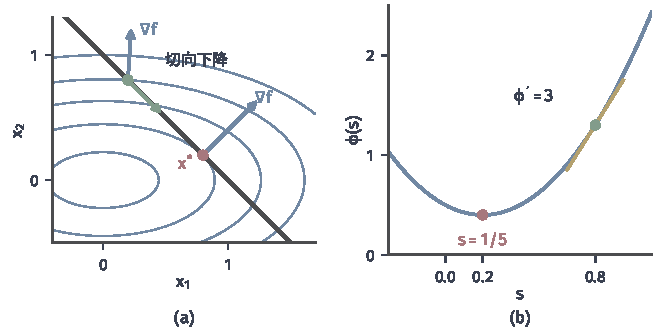
\includegraphics[width=112mm]{figures/05-optimization/06-constrained-optimization/matplotlib/kkt-equality-tangency/figure.pdf}
  \caption{等式约束问题~\eqref{eq:kkt-equality-qp}的切点条件。(a)蓝线是目标的等高线，深灰线是约束直线。红点$\bm{x}^\star=(4/5,1/5)$处直线与等高线相切，梯度沿法向。绿点$(0.2,0.8)$处梯度有切向分量，绿色箭头是沿直线的下降方向。(b)目标沿直线的限制$\phi(s)=f(1-s,s)$，红点是最小点$s=1/5$，绿点$s=0.8$处的切线（黄色）斜率为$3$。}
  \label{fig:kkt-equality-tangency}
\end{BookInlineFigure}

一般的等式约束情形完全一样，只是切向从一条线变成一个子空间。

\begin{theorem}[等式约束的一阶必要条件]
\label{thm:kkt-lagrange}
考虑只有等式约束的问题~\eqref{eq:kkt-problem}（$m=0$）。设$f$、$h_j$在局部最小点$\bm{x}^\star$附近连续可微，$\nabla h_1(\bm{x}^\star),\ldots,\nabla h_p(\bm{x}^\star)$线性无关。则存在唯一的$\bm{\nu}^\star\in\mathbb{R}^p$，使
\begin{equation}
 \nabla f(\bm{x}^\star)+\sum_{j=1}^p\nu_j^\star\nabla h_j(\bm{x}^\star)=\bm{0}.
 \label{eq:kkt-lagrange}
\end{equation}
\end{theorem}

\begin{proof}
以$\nabla h_j(\bm{x}^\star)^\top$为行组成矩阵$\bm{E}$。由定理~\ref{thm:kkt-licq-exact}，切锥等于线性化锥。这里线性化锥就是$\bm{E}$的零空间，是一个子空间。

由定理~\ref{thm:kkt-tangent-necessary}，对这个子空间中的$\bm{d}$有$\langle\nabla f(\bm{x}^\star),\bm{d}\rangle\geq0$。$-\bm{d}$也在子空间内，所以内积只能为零，即$\nabla f(\bm{x}^\star)$与$\bm{E}$的零空间正交。

零空间的正交补是$\bm{E}^\top$的值域，所以存在$\bm{u}$使$\nabla f(\bm{x}^\star)=\bm{E}^\top\bm{u}$，令$\bm{\nu}^\star=-\bm{u}$即得式~\eqref{eq:kkt-lagrange}。唯一性来自$\bm{E}^\top$的列线性无关。
\end{proof}

把目标和约束按乘子加权相加，定义\term{Lagrange函数}（Lagrangian）
\begin{equation}
 \mathcal{L}(\bm{x},\bm{\nu})=f(\bm{x})+\sum_{j=1}^p\nu_jh_j(\bm{x}).
 \label{eq:kkt-lagrangian-equality}
\end{equation}
式~\eqref{eq:kkt-lagrange}就是$\nabla_{\bm{x}}\mathcal{L}=\bm{0}$在$(\bm{x}^\star,\bm{\nu}^\star)$处成立，可行性$h_j=0$就是$\nabla_{\bm{\nu}}\mathcal{L}=\bm{0}$。约束问题的一阶条件由此写成了无约束形式的驻定方程。要注意，这只是驻定，$\mathcal{L}$在$\bm{x}^\star$不必取最小值，更不是在$(\bm{x},\bm{\nu})$上取最小值。

乘子还有一层经济含义。把例子的约束放松成$x_1+x_2=1+\varepsilon$，同样的计算给出最优值$\frac25(1+\varepsilon)^2$，它在$\varepsilon=0$处的导数是$4/5=-\nu$。所以$\lvert\nu\rvert$是约束右端变动一个单位时最优值的变化率，这叫影子价格。这里只是在一个例子上观察，一般结论和条件由第~\ref{chap:parametric-sensitivity}章讨论。

\subsection{不等式约束的KKT条件}
\label{sec:kkt-conditions}

等式约束的切向是子空间，$\bm{d}$和$-\bm{d}$都能走，所以乘子的符号不受限制。不等式只限制朝外的一侧，切向变成了锥，乘子应该带上符号。先用预算例看看符号是怎么来的。

\paragraph{力的平衡}
把$-\nabla f$想成目标施加在点上的拉力，把活动约束想成一堵墙。墙只能把点往内推，不能把点往外拉，第$i$堵墙的推力沿内法向，写成$-\lambda_i\nabla g_i$，其中$\lambda_i\geq0$是推力大小。不活动的约束碰不到点，推力为零。点在最优位置保持不动，意味着合力为零：
\begin{equation}
 -\nabla f(\bm{x}^\star)=\sum_{i\in A(\bm{x}^\star)}\lambda_i\nabla g_i(\bm{x}^\star),\qquad\lambda_i\geq0.
 \label{eq:kkt-force-balance}
\end{equation}
这个类比只解释一阶平衡，它不涉及动力学或曲率。等式约束是两面都有墙的轨道，推力可正可负，所以乘子不限号。

图~\ref{fig:kkt-force-balance}算了两个例子。$\tau=2$时只有预算线活动，$-\nabla f=(1/2,1/2)$，一堵墙就够了：$\lambda_1=1/2$。$\tau=1/2$时最优点在角点，两堵墙合力，由
\[
 \Bigl(\frac32,1\Bigr)=\lambda_1(1,1)+\lambda_3(0,-1)
\]
解出$\lambda_1=3/2$，$\lambda_3=1/2$，都非负。

\begin{BookInlineFigure}
  \centering
  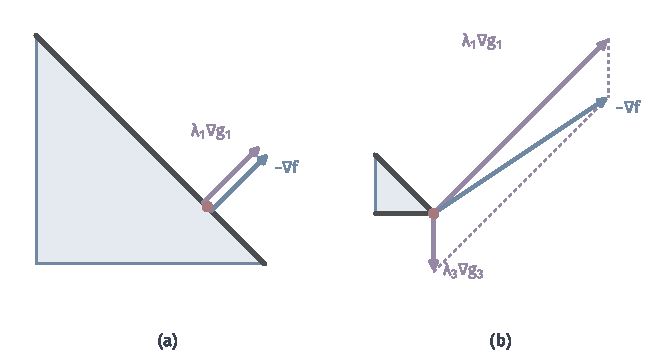
\includegraphics[width=112mm]{figures/05-optimization/06-constrained-optimization/matplotlib/kkt-force-balance/figure.pdf}
  \caption{最优点处的力的平衡。蓝色箭头是负梯度，紫色箭头是$\lambda_i\nabla g_i$。(a)$\tau=2$：$-\nabla f=\frac12\nabla g_1$（两箭头实际重合，为看清而错开绘制）。(b)$\tau=1/2$：$-\nabla f=\frac32\nabla g_1+\frac12\nabla g_3$，虚线组成平行四边形。}
  \label{fig:kkt-force-balance}
\end{BookInlineFigure}

\paragraph{从无下降方向到乘子}
力的平衡是直观，严格的推导要用第~\ref{chap:linear-programming}章的Farkas引理：对矩阵$\bm{M}$和向量$\bm{b}$，系统$\bm{M}\bm{u}=\bm{b}$，$\bm{u}\geq\bm{0}$与系统$\bm{M}^\top\bm{z}\geq\bm{0}$，$\bm{b}^\top\bm{z}<0$恰有一个有解。几何上，$\bm{b}$要么在$\bm{M}$的列张成的锥内，要么能被一个超平面与锥隔开。

\begin{lemma}[无线性化下降方向与乘子]
\label{lem:kkt-farkas}
设$\bar{\bm{x}}\in\bm{C}$，$f$与约束函数在$\bar{\bm{x}}$处可微。不存在$\bm{d}\in\bm{F}(\bar{\bm{x}})$使$\langle\nabla f(\bar{\bm{x}}),\bm{d}\rangle<0$，当且仅当存在$\lambda_i\geq0$（$i\in A(\bar{\bm{x}})$）和$\nu_j\in\mathbb{R}$，使
\begin{equation}
 \nabla f(\bar{\bm{x}})+\sum_{i\in A(\bar{\bm{x}})}\lambda_i\nabla g_i(\bar{\bm{x}})+\sum_{j=1}^p\nu_j\nabla h_j(\bar{\bm{x}})=\bm{0}.
 \label{eq:kkt-farkas-stationary}
\end{equation}
\end{lemma}

\begin{proof}
以活动的$\nabla g_i(\bar{\bm{x}})^\top$为行组成$\bm{B}$，以$\nabla h_j(\bar{\bm{x}})^\top$为行组成$\bm{E}$，在Farkas引理中取
\[
 \bm{M}=\begin{bmatrix}\bm{B}^\top&\bm{E}^\top&-\bm{E}^\top\end{bmatrix},\qquad\bm{b}=-\nabla f(\bar{\bm{x}}).
\]
把等式乘子拆成$\bm{\nu}=\bm{\nu}^{+}-\bm{\nu}^{-}$，两部分都非负，并记
\[
 \bm{u}=(\bm{\lambda}_A,\bm{\nu}^{+},\bm{\nu}^{-})\geq\bm{0},
\]
其中$\bm{\lambda}_A$是活动约束的乘子。方程$\bm{M}\bm{u}=\bm{b}$正是式~\eqref{eq:kkt-farkas-stationary}。

另一个系统要求$\bm{B}\bm{z}\geq\bm{0}$，$\bm{E}\bm{z}=\bm{0}$，$\langle\nabla f(\bar{\bm{x}}),\bm{z}\rangle>0$。令$\bm{d}=-\bm{z}$，它等价于
\[
 \bm{B}\bm{d}\leq\bm{0},\qquad\bm{E}\bm{d}=\bm{0},\qquad\langle\nabla f(\bar{\bm{x}}),\bm{d}\rangle<0,
\]
即存在线性化下降方向。Farkas引理说两个系统恰有一个有解，这就是要证的等价。
\end{proof}

图~\ref{fig:kkt-farkas-cone}画出引理的两种情形，两张图的约束梯度相同。(a)是$\tau=1/2$的角点，$-\nabla f$落在紫色的梯度锥内，乘子存在，绿色的线性化锥与它成钝角，没有下降方向。(b)是$\tau=2$时的角点$(2,0)$，这一点可行但不是最优点。这里$-\nabla f=(0,1)$在锥外。

解驻定方程$(0,-1)+\lambda_1(1,1)+\lambda_3(0,-1)=\bm{0}$，得$\lambda_1=0$，$\lambda_3=-1$，符号不对。负乘子正好指出了下降方向$\bm{d}=(-1,1)$，也就是离开$x_2=0$这堵墙：
\[
 f(2-s,s)=\frac12\bigl[s^2+(1-s)^2\bigr],\qquad\frac{\mathrm{d}}{\mathrm{d}s}f\Big|_{s=0}=-1<0.
\]

\begin{BookInlineFigure}
  \centering
  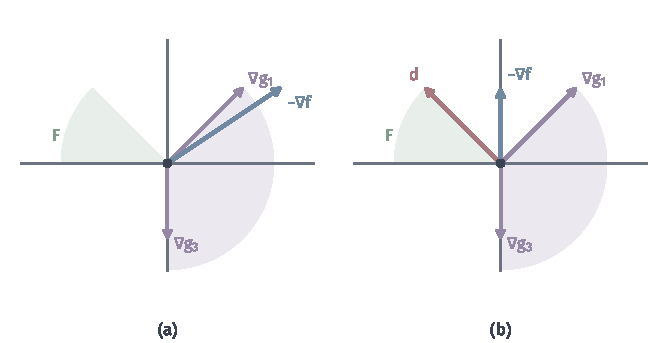
\includegraphics[width=112mm]{figures/05-optimization/06-constrained-optimization/matplotlib/kkt-farkas-cone/figure.pdf}
  \caption{Farkas引理的两种情形，画在方向空间中。紫色楔形是活动梯度张成的锥，浅绿楔形是线性化锥$\bm{F}$，蓝色箭头是$-\nabla f$。(a)$\tau=1/2$的角点：$-\nabla f=(3/2,1)$在锥内。(b)$\tau=2$的角点$(2,0)$：$-\nabla f=(0,1)$在锥外，红色箭头$\bm{d}=(-1,1)$在$\bm{F}$内，与负梯度成锐角，是下降方向。}
  \label{fig:kkt-farkas-cone}
\end{BookInlineFigure}

\paragraph{KKT条件}
式~\eqref{eq:kkt-farkas-stationary}只对活动约束求和。为了不必事先知道哪些约束活动，给每个不等式都配一个乘子，定义完整的Lagrange函数
\begin{equation}
 \mathcal{L}(\bm{x},\bm{\lambda},\bm{\nu})=f(\bm{x})+\sum_{i=1}^m\lambda_ig_i(\bm{x})+\sum_{j=1}^p\nu_jh_j(\bm{x}),
 \label{eq:kkt-lagrangian}
\end{equation}
并用乘积$\lambda_ig_i=0$规定“不活动的约束乘子为零”。这样就得到下面四组条件。

\begin{definition}[KKT条件]
\label{def:kkt-conditions}
设$f$、$g_i$、$h_j$在$\bm{x}^\star$处可微。若存在$\bm{\lambda}^\star\in\mathbb{R}^m$、$\bm{\nu}^\star\in\mathbb{R}^p$，使
\begin{align}
 &\nabla_{\bm{x}}\mathcal{L}(\bm{x}^\star,\bm{\lambda}^\star,\bm{\nu}^\star)=\bm{0}, \label{eq:kkt-stationarity}\\
 &g_i(\bm{x}^\star)\leq0,\quad h_j(\bm{x}^\star)=0, \label{eq:kkt-primal}\\
 &\lambda_i^\star\geq0, \label{eq:kkt-dual}\\
 &\lambda_i^\star g_i(\bm{x}^\star)=0, \label{eq:kkt-complementarity}
\end{align}
对所有$i=1,\ldots,m$，$j=1,\ldots,p$成立，就称$\bm{x}^\star$满足\term{KKT条件}（Karush--Kuhn--Tucker conditions），$(\bm{x}^\star,\bm{\lambda}^\star,\bm{\nu}^\star)$称为\term{KKT点}（KKT point），$(\bm{\lambda}^\star,\bm{\nu}^\star)$称为KKT乘子。
\end{definition}

表~\ref{tab:kkt-four-conditions}列出四组条件的分工。其中式~\eqref{eq:kkt-complementarity}称为互补松弛，它把活动集的选择藏进了乘积里。

\begin{BookInlineTable}
  \centering
  \begin{tabular}{@{}lll@{}}
    \toprule
    条件 & 式子 & 作用\\
    \midrule
    驻定 & \eqref{eq:kkt-stationarity} & 负梯度被约束的法向组合抵消\\
    原始可行 & \eqref{eq:kkt-primal} & 候选点满足全部约束\\
    乘子非负 & \eqref{eq:kkt-dual} & 墙只能推不能拉\\
    互补松弛 & \eqref{eq:kkt-complementarity} & 不活动约束不出力\\
    \bottomrule
  \end{tabular}
  \caption{KKT条件的四个组成部分。}
  \label{tab:kkt-four-conditions}
\end{BookInlineTable}

\paragraph{预算例的计算}
互补松弛把求解变成对活动集的枚举：猜一个活动集，令其余乘子为零，解方程，再检查可行性和符号。预算例的驻定条件是
\[
 x_1-2+\lambda_1-\lambda_2=0,\qquad x_2-1+\lambda_1-\lambda_3=0.
\]

取$\tau=2$。先猜没有活动约束，三个乘子都是零，得$\bm{x}=(2,1)$，但$g_1=1>0$，不可行。再猜只有$g_1$活动，$\lambda_2=\lambda_3=0$，$x_1+x_2=2$，由驻定条件得$x_1=2-\lambda_1$，$x_2=1-\lambda_1$，代入得
\[
 3-2\lambda_1=2,\qquad\lambda_1=\frac12,\qquad\bm{x}=\Bigl(\frac32,\frac12\Bigr).
\]
这一点可行，乘子非负，KKT条件全部成立。

取$\tau=1/2$。只有$g_1$活动时解出$\lambda_1=5/4$，$\bm{x}=(3/4,-1/4)$，不可行。再猜$g_1,g_3$活动，$x_2=0$，$x_1=1/2$，由第一个驻定方程得$\lambda_1=3/2$，第二个得$\lambda_3=\lambda_1-1=1/2$。全部条件成立。

让$\tau$连续变化，结果分三段：
\begin{equation}
 (\bm{x}^\star,\lambda_1,\lambda_3)=\begin{cases}
 \bigl((\tau,0),\ 2-\tau,\ 1-\tau\bigr),&0<\tau\leq1,\\
 \bigl((\tfrac{1+\tau}{2},\tfrac{\tau-1}{2}),\ \tfrac{3-\tau}{2},\ 0\bigr),&1\leq\tau\leq3,\\
 \bigl((2,1),\ 0,\ 0\bigr),&\tau\geq3,
 \end{cases}
 \label{eq:kkt-budget-solution}
\end{equation}
三段都有$\lambda_2=0$。图~\ref{fig:kkt-tau-regimes}画出最优点的轨迹和乘子曲线。

\begin{BookInlineFigure}
  \centering
  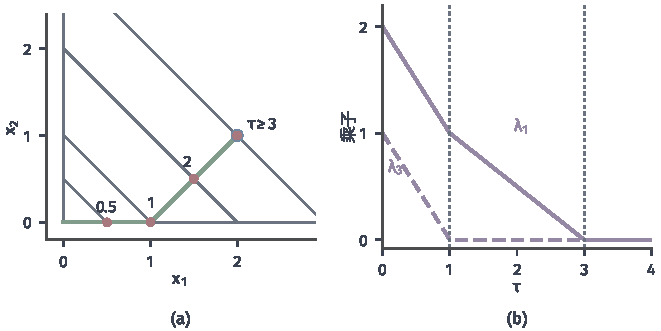
\includegraphics[width=112mm]{figures/05-optimization/06-constrained-optimization/matplotlib/kkt-tau-regimes/figure.pdf}
  \caption{预算例的解随$\tau$变化。(a)绿线是最优点轨迹，深灰细线是预算线$x_1+x_2=\tau$，红点对应$\tau=0.5,1,2,3$，空心点是$\bm{c}$。(b)乘子$\lambda_1$（实线）与$\lambda_3$（虚线），竖直虚线是活动集改变的位置$\tau=1,3$。}
  \label{fig:kkt-tau-regimes}
\end{BookInlineFigure}

这个例子说清了互补松弛的方向。$\lambda_i>0$推出约束活动，但约束活动推不出$\lambda_i>0$。$\tau=3$时预算线恰好经过$\bm{c}$，$g_1$活动，而$\lambda_1=0$：预算恰好够用，这堵墙碰到了点却不用出力。$\tau=1$时最优点是角点$(1,0)$，$g_3$活动，$\lambda_3=0$，同样如此。

从公式~\eqref{eq:kkt-budget-solution}还能再次看到影子价格。$1\leq\tau\leq3$时最优值是$(3-\tau)^2/4$，它对$\tau$的导数是$-(3-\tau)/2=-\lambda_1$：多一块钱，目标改善$\lambda_1$。

\subsection{乘子的存在与唯一性}
\label{sec:kkt-existence}

前面的推导把各步准备好了，现在把它们合起来。

\begin{theorem}[KKT条件的必要性]
\label{thm:kkt-necessary}
设$f$、$g_i$、$h_j$在局部最小点$\bm{x}^\star$附近连续可微。若$\bm{x}^\star$满足MFCQ，则存在KKT乘子$(\bm{\lambda}^\star,\bm{\nu}^\star)$，并且全体KKT乘子组成有界集合。若$\bm{x}^\star$满足LICQ，则KKT乘子唯一。
\end{theorem}

\begin{proof}
\emph{存在性。}由定理~\ref{thm:kkt-mfcq-exact}，切锥等于线性化锥。由定理~\ref{thm:kkt-tangent-necessary}，$\bm{F}(\bm{x}^\star)$中没有使$\langle\nabla f(\bm{x}^\star),\bm{d}\rangle<0$的方向。引理~\ref{lem:kkt-farkas}给出活动约束的乘子与$\bm{\nu}^\star$。不活动约束的乘子取零，四组条件全部成立。

\emph{有界性。}若乘子列$(\bm{\lambda}^{(k)},\bm{\nu}^{(k)})$的范数趋于无穷，把驻定方程除以这个范数，取收敛子列，极限$(\bar{\bm{\lambda}},\bar{\bm{\nu}})$的范数为$1$，满足$\bar{\bm{\lambda}}\geq\bm{0}$，不活动分量为零，并且
\[
 \sum_{i\in A(\bm{x}^\star)}\bar{\lambda}_i\nabla g_i(\bm{x}^\star)+\sum_{j=1}^p\bar{\nu}_j\nabla h_j(\bm{x}^\star)=\bm{0}.
\]

把上式与MFCQ的方向$\bar{\bm{d}}$作内积，等式项消失，得到
\[
 \sum_{i\in A(\bm{x}^\star)}\bar{\lambda}_i\langle\nabla g_i(\bm{x}^\star),\bar{\bm{d}}\rangle=0.
\]
每项都非正，而内积严格为负，所以$\bar{\bm{\lambda}}=\bm{0}$。剩下的等式项由$\nabla h_j$线性无关推出$\bar{\bm{\nu}}=\bm{0}$，与范数为$1$矛盾。

\emph{唯一性。}设有两组KKT乘子。不活动分量都是零，两个驻定方程相减，得到活动梯度和等式梯度的一个线性组合等于零，系数是两组乘子之差。LICQ说明系数全为零。
\end{proof}

由引理~\ref{lem:kkt-licq-implies-mfcq}，LICQ下存在性自动成立。全部活动约束与等式约束都是仿射函数时，$\bm{T}_{\bm{C}}=\bm{F}$不需要任何资格，乘子同样存在，只是有界性和唯一性不再有保证。

\paragraph{存在与唯一是两回事}
图~\ref{fig:kkt-multiplier-sets}对比几种情形的乘子集合。把预算线写两遍（$\tau=2$），MFCQ成立，驻定条件只约束$\lambda_1+\lambda_1'$的和，$\lambda_1+\lambda_1'=1/2$是一条线段：乘子存在、有界，但不唯一。

再看在$\{0\}$上最小化$x$。写成$x\leq0$，$-x\leq0$时，驻定方程是$1+\lambda_1-\lambda_2=0$，解集是无界射线，MFCQ不成立时有界性确实可能失去。写成$x=0$时，$\nu=-1$是唯一乘子。

\paragraph{没有乘子的最小点}
第三种写法最值得注意。最小化$x$，约束$g(x)=x^2\leq0$。可行集只有原点，所以$x^\star=0$是全局最小点。驻定方程是
\[
 1+\lambda\cdot2x^\star=1=0,
\]
对任何$\lambda$都无解，图~\ref{fig:kkt-multiplier-sets}(c)的残差恒为$1$。这是一个没有KKT乘子的最小点。

因此，不能仅凭驻定方程无解就排除一个候选点，除非已经确认它满足约束资格。这里的问题出在约束函数的写法上，$\nabla g(0)=0$让约束的一阶信息完全失效，与目标函数无关。

\begin{BookInlineFigure}
  \centering
  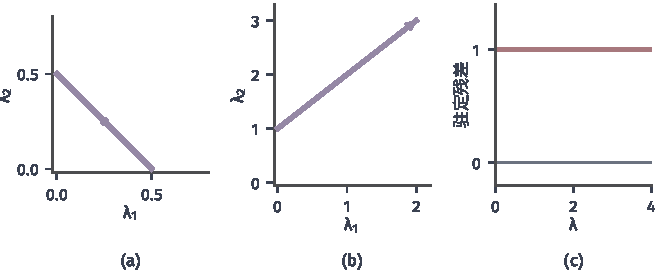
\includegraphics[width=112mm]{figures/05-optimization/06-constrained-optimization/matplotlib/kkt-multiplier-sets/figure.pdf}
  \caption{KKT乘子集合的三种情况。(a)预算线写两遍（$\tau=2$），乘子集合是线段$\lambda_1+\lambda_2=1/2$（这里$\lambda_2$表示重复约束的乘子），有界而不唯一。(b)$\min x$，约束$x\leq0$，$-x\leq0$：乘子集合是无界射线$\lambda_2=1+\lambda_1$。(c)$\min x$，约束$x^2\leq0$：对任何乘子，驻定残差都等于$1$，乘子不存在。}
  \label{fig:kkt-multiplier-sets}
\end{BookInlineFigure}

\subsection{凸问题的全局判别}
\label{sec:kkt-convex}

KKT条件在约束资格下是必要的，它能筛掉不合格的点，却不能确认合格的点就是最小点。什么时候能反过来？答案是问题凸的时候，而且这时连约束资格都不用检查。

\begin{theorem}[凸问题的KKT充分性]
\label{thm:kkt-convex-sufficient}
设$\bm{D}\subseteq\mathbb{R}^n$是包含可行集的开凸集，$f$与$g_i$在$\bm{D}$上凸且可微，$h_j$是仿射函数。若$(\bm{x}^\star,\bm{\lambda}^\star,\bm{\nu}^\star)$是KKT点，则$\bm{x}^\star$是问题~\eqref{eq:kkt-problem}的全局最小点。
\end{theorem}

\begin{proof}
任取可行点$\bm{x}$，记$\bm{u}=\bm{x}-\bm{x}^\star$。由第~\ref{chap:optimization}章的一阶支撑不等式，凸函数$f$满足
\[
 f(\bm{x})\geq f(\bm{x}^\star)+\langle\nabla f(\bm{x}^\star),\bm{u}\rangle.
\]
再由驻定条件~\eqref{eq:kkt-stationarity}，把梯度替换掉：
\[
 f(\bm{x})\geq f(\bm{x}^\star)-\sum_{i=1}^m\lambda_i^\star\langle\nabla g_i(\bm{x}^\star),\bm{u}\rangle-\sum_{j=1}^p\nu_j^\star\langle\nabla h_j(\bm{x}^\star),\bm{u}\rangle.
\]

$h_j$仿射，$\bm{x}$与$\bm{x}^\star$都可行，所以
\[
 \langle\nabla h_j(\bm{x}^\star),\bm{u}\rangle=h_j(\bm{x})-h_j(\bm{x}^\star)=0,
\]
最后一个和式消失。

对$\lambda_i^\star=0$的项，这一项本来就是零。对$\lambda_i^\star>0$的项，互补松弛给出$g_i(\bm{x}^\star)=0$，再对凸函数$g_i$用支撑不等式：
\[
 \langle\nabla g_i(\bm{x}^\star),\bm{u}\rangle\leq g_i(\bm{x})-g_i(\bm{x}^\star)=g_i(\bm{x})\leq0.
\]
所以和式中每一项$-\lambda_i^\star\langle\nabla g_i,\bm{u}\rangle$都非负，代回得到$f(\bm{x})\geq f(\bm{x}^\star)$。
\end{proof}

证明的每一步都用到了相应的假设：目标凸给出一个全局下界，$g_i$凸把梯度内积换成函数值，乘子非负保证不等号的方向，互补松弛消去$g_i(\bm{x}^\star)$，等式仿射让等式项消失。

把它用在预算例上。目标凸，约束都是仿射函数，所以式~\eqref{eq:kkt-budget-solution}中的点都是全局最小点，这一步不需要再检查什么。

还可以从Lagrange函数看这个结论。固定乘子后，$\mathcal{L}(\cdot,\bm{\lambda}^\star,\bm{\nu}^\star)$是凸函数，驻定点就是它的全局最小点。在可行点上$\mathcal{L}\leq f$，在$\bm{x}^\star$处两者相等，于是目标在$\bm{x}^\star$被一个碗从下面托住了。图~\ref{fig:kkt-convex-vs-nonconvex}(a)取最小化$(x-2)^2$、约束$x-1\leq0$的问题，$x^\star=1$，$\lambda^\star=2$，$\mathcal{L}(x,2)=(x-1)^2+1$就是紫色的碗，可行域上它在$f$的下方。

\begin{BookInlineFigure}
  \centering
  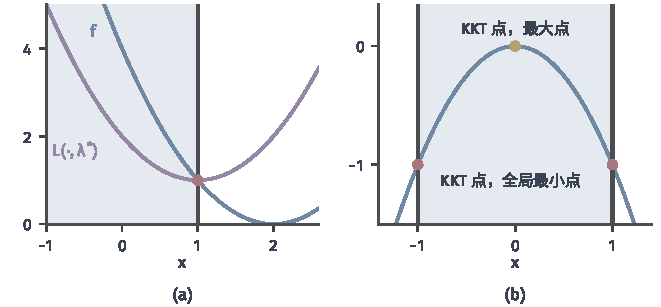
\includegraphics[width=112mm]{figures/05-optimization/06-constrained-optimization/matplotlib/kkt-convex-vs-nonconvex/figure.pdf}
  \caption{凸与非凸问题中的KKT点。浅蓝带是可行域，深灰线是活动约束的位置。(a)$\min(x-2)^2$，$x\leq1$：KKT点$x^\star=1$（红），$\lambda^\star=2$。紫色曲线$\mathcal{L}(x,2)=(x-1)^2+1$在可行域上位于$f$（蓝）下方，并在$x^\star$处与$f$相接。(b)$\min-x^2$，$\lvert x\rvert\leq1$：三个KKT点中$x=0$（黄）是最大点，$x=\pm1$（红）是全局最小点。}
  \label{fig:kkt-convex-vs-nonconvex}
\end{BookInlineFigure}

\paragraph{去掉凸性会怎样}
一般非凸问题中，KKT条件只提供候选。在$[-1,1]$上最小化$-x^2$，约束写成$x-1\leq0$，$-x-1\leq0$。点$x=0$没有活动约束，$f'(0)=0$，乘子取零就满足KKT条件，但它是全局最大点。点$x=1$处由$-2+\lambda_1=0$得$\lambda_1=2$，也满足KKT条件，它才是最小点。KKT方程分不开这两种点，见图~\ref{fig:kkt-convex-vs-nonconvex}(b)。

等式必须是仿射函数也不是多余的要求。单位圆周的$h(\bm{x})=x_1^2+x_2^2-1$是凸函数，目标$\frac12\lVert\bm{x}-(2,0)\rVert_2^2$也是凸函数，但$(-1,0)$是KKT点，却是圆周上的全局最大点。$h=0$的解集不是凸集，定理的证明在处理等式项那一步就失效了。

另外，充分性不提供存在性。$\min x$，$x^2\leq0$是凸问题，最小点却没有KKT乘子。表~\ref{tab:kkt-necessity-sufficiency}把必要性与充分性的条件放在一起。

\begin{BookInlineTable}
  \centering
  \begin{tabular}{@{}lll@{}}
    \toprule
    结论方向 & 所需条件 & 结论\\
    \midrule
    局部最小$\Rightarrow$KKT & MFCQ（或LICQ、仿射约束） & 存在乘子\\
    KKT$\Rightarrow$全局最小 & 目标、$g_i$凸，$h_j$仿射 & 不需要约束资格\\
    KKT$\Rightarrow$局部最小 & 一般不成立 & 需要二阶条件\\
    \bottomrule
  \end{tabular}
  \caption{KKT条件的必要性与充分性。}
  \label{tab:kkt-necessity-sufficiency}
\end{BookInlineTable}

\section{二阶条件}
\label{sec:kkt-second-order}

KKT点可能是最小点，也可能不是。单位圆周上最小化$\frac12\lVert\bm{x}-(2,0)\rVert_2^2$就是例子：离$(2,0)$最近和最远的点都满足一阶条件。这就需要回答：一阶信息判断不了的时候，曲率怎样作出判断？这需要先确定该检查哪些方向，再确定该检查谁的曲率。

\subsection{临界锥}
\label{sec:kkt-critical-cone}

设$(\bm{x}^\star,\bm{\lambda}^\star,\bm{\nu}^\star)$是KKT点。对线性化方向$\bm{d}\in\bm{F}(\bm{x}^\star)$，由驻定条件，目标的一阶变化是
\[
 \langle\nabla f(\bm{x}^\star),\bm{d}\rangle=-\sum_{i\in A(\bm{x}^\star)}\lambda_i^\star\langle\nabla g_i(\bm{x}^\star),\bm{d}\rangle-\sum_{j=1}^p\nu_j^\star\langle\nabla h_j(\bm{x}^\star),\bm{d}\rangle.
\]
等式项为零。每个$\lambda_i^\star\geq0$，每个$\langle\nabla g_i,\bm{d}\rangle\leq0$，所以右端是非负项之和。

若这个值严格为正，目标沿$\bm{d}$一阶上升，这个方向已经判决完毕，二阶项不用看。需要继续检查的，只有一阶变化恰好为零的方向。一个非负项之和为零，当且仅当每一项为零，所以这些方向在$\lambda_i^\star>0$的活动约束上必须取等号。

\begin{definition}[临界锥]
\label{def:kkt-critical-cone}
设$(\bm{x}^\star,\bm{\lambda}^\star,\bm{\nu}^\star)$是KKT点。集合
\begin{equation}
 \bm{K}(\bm{x}^\star,\bm{\lambda}^\star)=\left\{\bm{d}\in\bm{F}(\bm{x}^\star):
 \langle\nabla g_i(\bm{x}^\star),\bm{d}\rangle=0\ \text{对所有}\ \lambda_i^\star>0
 \right\}
 \label{eq:kkt-critical-cone}
\end{equation}
称为\term{临界锥}（critical cone）。由上面的推导，它等于
\begin{equation}
 \bm{K}(\bm{x}^\star,\bm{\lambda}^\star)=\{\bm{d}\in\bm{F}(\bm{x}^\star):\langle\nabla f(\bm{x}^\star),\bm{d}\rangle=0\}.
 \label{eq:kkt-critical-cone-f}
\end{equation}
\end{definition}

式~\eqref{eq:kkt-critical-cone-f}的右端不含乘子，所以即使乘子不唯一，临界锥也不依赖乘子的选择。两种写法各有用处：式~\eqref{eq:kkt-critical-cone}便于计算，式~\eqref{eq:kkt-critical-cone-f}说明它的含义。

零乘子的活动约束值得单独看。这样的约束在式~\eqref{eq:kkt-critical-cone}里没有被要求取等号，它仍然保留$\langle\nabla g_i,\bm{d}\rangle\leq0$的单侧限制。所以临界锥一般是锥，不是子空间。

用预算例算三种情况，见图~\ref{fig:kkt-critical-cone}。$\tau=1/2$的角点，$\lambda_1,\lambda_3$都为正，两条约束都取等号，$d_1+d_2=0$，$d_2=0$，于是$\bm{K}=\{\bm{0}\}$：一阶条件已经判决了所有方向。

$\tau=1$的角点$(1,0)$，$\lambda_1=1>0$，$\lambda_3=0$，于是$g_1$取等号，$g_3$只保留单侧：
\[
 \bm{K}=\{\bm{d}:d_1+d_2=0,\ d_2\geq0\}=\{s(-1,1):s\geq0\}.
\]
沿预算线向上走的这一条射线，一阶变化为零，要靠二阶项判断。而反方向$(1,-1)$不可行。

\begin{BookInlineFigure}
  \centering
  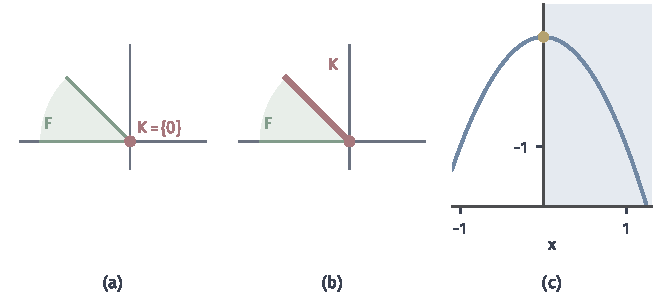
\includegraphics[width=112mm]{figures/05-optimization/06-constrained-optimization/matplotlib/kkt-critical-cone/figure.pdf}
  \caption{临界锥（红色）与线性化锥$\bm{F}$（绿色）。(a)预算例$\tau=1/2$的角点，两个乘子都为正，$\bm{K}=\{\bm{0}\}$。(b)预算例$\tau=1$的角点，$\lambda_3=0$，$\bm{K}$是射线$s(-1,1)$，$s\geq0$。(c)$\min-x^2$，$x\geq0$（蓝色带），黄点$x=0$是KKT点，乘子为零，$\bm{K}=[0,\infty)$。}
  \label{fig:kkt-critical-cone}
\end{BookInlineFigure}

\paragraph{不能把活动约束都当成等式}
一种常见的简化是把所有活动约束当成等式，对每个活动的$g_i$都要求$\langle\nabla g_i,\bm{d}\rangle=0$。下面的例子说明这样会漏掉下降方向。最小化$f(x)=-x^2$，约束$g(x)=-x\leq0$。在$x=0$处，$f'(0)=0$，所以$\lambda=0$，KKT条件成立。

约束活动而乘子为零，真正的临界锥是$\{d:-d\leq0\}=[0,\infty)$。沿$d=1$，$f''(0)d^2=-2<0$，二阶检验发现$x=0$不是局部最小点，事实上$f(t)=-t^2<0$。

要是把约束当成等式，方向只剩$\{0\}$，就没有方向可供检查，会错误地接受$x=0$。图~\ref{fig:kkt-critical-cone}(c)就是这个例子。

\subsection{二阶必要条件}
\label{sec:kkt-sonc}

下一个问题是该检查谁的曲率。答案不是目标的Hessian，用下面的例子就能看清。

\paragraph{约束的弯曲进入曲率}
在单位圆周上最小化$f(\bm{x})=\frac12[(x_1-2)^2+x_2^2]$，也就是找圆周上离$(2,0)$最近的点。令$h(\bm{x})=x_1^2+x_2^2-1$，驻定条件是
\[
 x_1-2+2\nu x_1=0,\qquad x_2+2\nu x_2=0.
\]
第二式说明$x_2=0$或$\nu=-1/2$。后者代入第一式得$-2=0$，不可能，所以$x_2=0$，$x_1=\pm1$。两个KKT点是
\[
 (1,0),\ \nu=\frac12;\qquad(-1,0),\ \nu=-\frac32.
\]

这两点的目标Hessian都是单位阵，正定，分不开。用角度参数化圆周，目标变成
\[
 \phi(\theta)=f(\cos\theta,\sin\theta)=\frac52-2\cos\theta,\qquad\phi''(\theta)=2\cos\theta.
\]
在$(1,0)$处$\phi''=2$，是极小；在$(-1,0)$处$\phi''=-2$，是极大。图~\ref{fig:kkt-constraint-curvature}(b)的黄色抛物线就是这两个曲率。

\begin{BookInlineFigure}
  \centering
  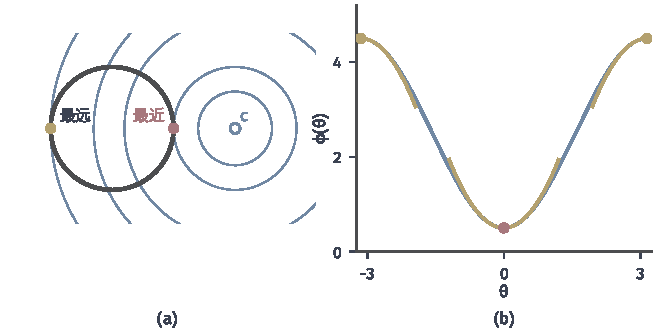
\includegraphics[width=112mm]{figures/05-optimization/06-constrained-optimization/matplotlib/kkt-constraint-curvature/figure.pdf}
  \caption{约束的弯曲改变了有效曲率。(a)深灰圆是可行集，蓝线是目标$\frac12\lVert\bm{x}-\bm{c}\rVert_2^2$（$\bm{c}=(2,0)$）的等高线。红点$(1,0)$是最近点，黄点$(-1,0)$是最远点，两者都是KKT点，目标Hessian都是单位阵。(b)沿圆周的目标值$\phi(\theta)=5/2-2\cos\theta$，黄色抛物线是两点处曲率分别为$2$、$-2$的二次近似。}
  \label{fig:kkt-constraint-curvature}
\end{BookInlineFigure}

这两个数从哪里来？沿可行曲线$\bm{x}(t)$，$\bm{x}(0)=\bm{x}^\star$，$\bm{x}'(0)=\bm{d}$，复合函数求二阶导数得到
\[
 \frac{\mathrm{d}^2}{\mathrm{d}t^2}f(\bm{x}(t))\Big|_{t=0}=\bm{d}^\top\nabla^2f(\bm{x}^\star)\bm{d}+\langle\nabla f(\bm{x}^\star),\bm{x}''(0)\rangle.
\]
第二项是曲线的弯曲$\bm{x}''(0)$贡献的，它是约束带来的，只看目标Hessian看不到这一项。

对恒等式$h(\bm{x}(t))=0$同样求两次导数，得到
\[
 \bm{d}^\top\nabla^2h(\bm{x}^\star)\bm{d}+\langle\nabla h(\bm{x}^\star),\bm{x}''(0)\rangle=0.
\]
再由驻定条件$\nabla f=-\nu\nabla h$，弯曲项可以用约束的Hessian表示：
\[
 \langle\nabla f(\bm{x}^\star),\bm{x}''(0)\rangle=-\nu\langle\nabla h(\bm{x}^\star),\bm{x}''(0)\rangle=\nu\,\bm{d}^\top\nabla^2h(\bm{x}^\star)\bm{d}.
\]

两式合起来，沿曲线的二阶导数恰好是
\[
 \bm{d}^\top\bigl(\nabla^2f(\bm{x}^\star)+\nu\nabla^2h(\bm{x}^\star)\bigr)\bm{d},
\]
括号里是Lagrange函数对$\bm{x}$的Hessian。乘子把约束的弯曲折算成了目标的曲率。在例子中$\nabla^2h=2\bm{I}$，$\bm{d}=(0,1)$，代入$(1,0)$得$1+2\cdot\frac12=2$，代入$(-1,0)$得$1+2\cdot(-\frac32)=-2$，与$\phi''$完全一致。

一般地，把Lagrange函数对$\bm{x}$的Hessian记为
\begin{equation}
 \nabla^2_{\bm{x}\bm{x}}\mathcal{L}(\bm{x},\bm{\lambda},\bm{\nu})=\nabla^2f(\bm{x})+\sum_{i=1}^m\lambda_i\nabla^2g_i(\bm{x})+\sum_{j=1}^p\nu_j\nabla^2h_j(\bm{x}).
 \label{eq:kkt-lagrangian-hessian}
\end{equation}

\begin{theorem}[二阶必要条件]
\label{thm:kkt-sonc}
设$f$、$g_i$、$h_j$在局部最小点$\bm{x}^\star$附近二阶连续可微，$\bm{x}^\star$满足LICQ，$(\bm{\lambda}^\star,\bm{\nu}^\star)$是它唯一的KKT乘子。则
\begin{equation}
 \bm{d}^\top\nabla^2_{\bm{x}\bm{x}}\mathcal{L}(\bm{x}^\star,\bm{\lambda}^\star,\bm{\nu}^\star)\bm{d}\geq0
 \quad\text{对所有}\ \bm{d}\in\bm{K}(\bm{x}^\star,\bm{\lambda}^\star).
 \label{eq:kkt-sonc}
\end{equation}
\end{theorem}

\begin{proof}
取$\bm{d}\in\bm{K}$，令
\[
 W=\{i\in A(\bm{x}^\star):\langle\nabla g_i(\bm{x}^\star),\bm{d}\rangle=0\}.
\]
由临界锥的定义，$\lambda_i^\star>0$的下标都在$W$中。LICQ保证引理~\ref{lem:kkt-feasible-curve}适用，得到二阶连续可微的可行曲线$\bm{x}(t)$，$0\leq t<\delta$，它沿$\bm{d}$出发，并使$h_j$与$g_i$（$i\in W$）恒为零。

令$\phi(t)$是乘子固定为$(\bm{\lambda}^\star,\bm{\nu}^\star)$时Lagrange函数沿曲线的值。曲线上等式约束为零，$i\in W$的约束为零，其余约束的乘子为零，所以对$0\leq t<\delta$，
\[
 \phi(t)=\mathcal{L}(\bm{x}(t),\bm{\lambda}^\star,\bm{\nu}^\star)=f(\bm{x}(t)).
\]
这是使用Lagrange函数的好处：在这条曲线上，它和目标完全一样，但它的梯度在$\bm{x}^\star$处为零。

由驻定条件，
\[
 \phi'(0)=\langle\nabla_{\bm{x}}\mathcal{L}(\bm{x}^\star,\bm{\lambda}^\star,\bm{\nu}^\star),\bm{d}\rangle=0.
\]
再求一次导数，含$\bm{x}''(0)$的项同样因$\nabla_{\bm{x}}\mathcal{L}=\bm{0}$消失，得到
\[
 \phi''(0)=\bm{d}^\top\nabla^2_{\bm{x}\bm{x}}\mathcal{L}(\bm{x}^\star,\bm{\lambda}^\star,\bm{\nu}^\star)\bm{d}.
\]

$\bm{x}(t)$可行且趋于局部最小点，所以小的$t>0$时$\phi(t)\geq\phi(0)$。由Taylor公式，$\phi(t)-\phi(0)=\frac12\phi''(0)t^2+o(t^2)$，除以$t^2$并令$t\downarrow0$，得到$\phi''(0)\geq0$。
\end{proof}

定理中的LICQ负责把每个临界方向实现成可行曲线。没有约束资格时，临界方向可能只是线性化的产物。最小化$-x^2$，约束$x^2\leq0$，原点是唯一可行点，取乘子$\lambda=0$是一组KKT乘子，此时$\nabla^2_{xx}\mathcal{L}=-2$，$\bm{K}=\mathbb{R}$，式~\eqref{eq:kkt-sonc}不成立，而原点当然是最小点。

\paragraph{两种错误的简化}
条件~\eqref{eq:kkt-sonc}既不等同于目标Hessian半正定，也不等同于在全空间半正定。圆周例已经说明目标Hessian可以正定而点不是局部最小点。

反过来，全空间的不定性也不妨碍极小。最小化$x_1^2-x_2^2$，约束$x_2=0$，原点处$\nu=0$，Lagrange Hessian是$\operatorname{diag}(2,-2)$，不定。但临界锥是$\{\bm{d}:d_2=0\}$，上面的二次型是$2d_1^2\geq0$。原点确实是最小点，负曲率的方向被约束禁止了。

\subsection{二阶充分条件}
\label{sec:kkt-sosc}

必要条件是用来排除的，充分条件是用来确认的。把不等号换成严格，就能确认局部最优，并且还能给出增长的速度。值得注意的是，这里不需要约束资格。

\begin{theorem}[二阶充分条件]
\label{thm:kkt-sosc}
设$f$、$g_i$、$h_j$在$\bm{x}^\star$附近二阶连续可微，$(\bm{x}^\star,\bm{\lambda}^\star,\bm{\nu}^\star)$是KKT点，并且
\begin{equation}
 \bm{d}^\top\nabla^2_{\bm{x}\bm{x}}\mathcal{L}(\bm{x}^\star,\bm{\lambda}^\star,\bm{\nu}^\star)\bm{d}>0
 \quad\text{对所有非零}\ \bm{d}\in\bm{K}(\bm{x}^\star,\bm{\lambda}^\star).
 \label{eq:kkt-sosc}
\end{equation}
则存在$\sigma>0$，$r>0$，使
\begin{equation}
 f(\bm{x})\geq f(\bm{x}^\star)+\sigma\lVert\bm{x}-\bm{x}^\star\rVert_2^2
 \quad\text{对所有}\ \bm{x}\in\bm{C},\ \lVert\bm{x}-\bm{x}^\star\rVert_2<r.
 \label{eq:kkt-quadratic-growth}
\end{equation}
特别地，$\bm{x}^\star$是严格局部最小点。
\end{theorem}

\begin{proof}
反设结论不成立。对每个$k$取$\sigma=1/k$，存在可行点$\bm{x}^{(k)}\neq\bm{x}^\star$，$\bm{x}^{(k)}\to\bm{x}^\star$，使
\[
 f(\bm{x}^{(k)})<f(\bm{x}^\star)+\frac1k\lVert\bm{x}^{(k)}-\bm{x}^\star\rVert_2^2.
\]
记$t_k=\lVert\bm{x}^{(k)}-\bm{x}^\star\rVert_2$，$\bm{d}^{(k)}=(\bm{x}^{(k)}-\bm{x}^\star)/t_k$。单位向量列有收敛子列，不妨设$\bm{d}^{(k)}\to\bm{d}$，$\lVert\bm{d}\rVert_2=1$。按定义~\ref{def:kkt-tangent-cone}，$\bm{d}$是切向量，由定理~\ref{thm:kkt-tangent-in-linearized}，$\bm{d}\in\bm{F}(\bm{x}^\star)$。

\emph{第一步：$\bm{d}$是临界方向。}上面的不等式减去$f(\bm{x}^\star)$，除以$t_k$，令$k\to\infty$，得到$\langle\nabla f(\bm{x}^\star),\bm{d}\rangle\leq0$。第~\ref{sec:kkt-critical-cone}节已经证明，$\bm{d}\in\bm{F}$时这个内积是非负项之和，所以它等于零。由式~\eqref{eq:kkt-critical-cone-f}，$\bm{d}\in\bm{K}$。

\emph{第二步：比较Lagrange函数。}下面乘子固定为$(\bm{\lambda}^\star,\bm{\nu}^\star)$，把Lagrange函数简记为$\mathcal{L}(\bm{x})$。$\bm{x}^{(k)}$可行，$\bm{\lambda}^\star\geq\bm{0}$，所以$\mathcal{L}(\bm{x}^{(k)})\leq f(\bm{x}^{(k)})$。由互补松弛和等式约束，$\mathcal{L}(\bm{x}^\star)=f(\bm{x}^\star)$。于是
\[
 \mathcal{L}(\bm{x}^{(k)})-\mathcal{L}(\bm{x}^\star)\leq f(\bm{x}^{(k)})-f(\bm{x}^\star)<\frac{t_k^2}{k}.
\]

\emph{第三步：展开。}在$\bm{x}^\star$处$\nabla_{\bm{x}}\mathcal{L}=\bm{0}$，由二阶Taylor公式，
\[
 \mathcal{L}(\bm{x}^{(k)})-\mathcal{L}(\bm{x}^\star)=\frac{t_k^2}{2}(\bm{d}^{(k)})^\top\nabla^2_{\bm{x}\bm{x}}\mathcal{L}(\bm{x}^\star)\bm{d}^{(k)}+o(t_k^2).
\]
代入上式，除以$t_k^2$，令$k\to\infty$，得到
\[
 \frac12\bm{d}^\top\nabla^2_{\bm{x}\bm{x}}\mathcal{L}(\bm{x}^\star)\bm{d}\leq0.
\]
这与式~\eqref{eq:kkt-sosc}矛盾。
\end{proof}

证明从头到尾没有用到切锥等于线性化锥，只用了$\bm{T}_{\bm{C}}\subseteq\bm{F}$这个总成立的方向，所以不需要约束资格。它也只要求某一组KKT乘子满足式~\eqref{eq:kkt-sosc}。

在圆周的最近点$(1,0)$，$\bm{K}=\{(0,s)\}$，$\nabla^2_{\bm{x}\bm{x}}\mathcal{L}=2\bm{I}$，条件成立。这里增长式可以精确写出。圆周上，
\[
 f(\bm{x})-\frac12=2-2\cos\theta=\lVert\bm{x}-(1,0)\rVert_2^2,
\]
所以$\sigma=1$。

临界锥只有零向量时，条件~\eqref{eq:kkt-sosc}自动成立，这时一阶条件就足以确认严格局部最小。预算例$\tau=1/2$的角点就是这样。

\paragraph{条件的边界}
严格正性不能放松成半正定。图~\ref{fig:kkt-degenerate-curvature}中三个一元函数在原点的二阶导数都是零，临界锥都是全空间，半正定都成立，可是$x^3$和$-x^4$的原点都不是局部最小点。

严格正性也不是必要的。$x^4$的原点是严格局部最小点，二阶导数却是零。所以二阶必要条件和二阶充分条件之间有一条缝，缝里的情形要靠更高阶的信息或问题的特殊结构。

\begin{BookInlineFigure}
  \centering
  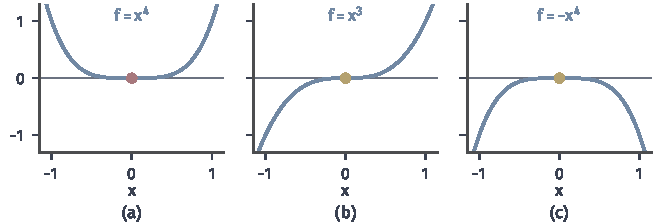
\includegraphics[width=112mm]{figures/05-optimization/06-constrained-optimization/matplotlib/kkt-degenerate-curvature/figure.pdf}
  \caption{二阶导数为零时，二阶条件无法判决。(a)$x^4$：原点（红）是严格局部最小点。(b)$x^3$：原点（黄）不是局部极值点。(c)$-x^4$：原点（黄）是最大点。三者在原点的一、二阶导数都是零。}
  \label{fig:kkt-degenerate-curvature}
\end{BookInlineFigure}

表~\ref{tab:kkt-second-order}对比这两个条件。

\begin{BookInlineTable}
  \centering
  \begin{tabular}{@{}lll@{}}
    \toprule
    对比项 & 二阶必要条件 & 二阶充分条件\\
    \midrule
    出发点 & 已知局部最小点 & 已知KKT点\\
    约束资格 & 需要LICQ & 不需要\\
    二次型 & 在$\bm{K}$上$\geq0$ & 在$\bm{K}$的非零向量上$>0$\\
    结论 & 用于排除候选点 & 严格局部最小，二次增长\\
    \bottomrule
  \end{tabular}
  \caption{二阶必要条件与二阶充分条件的比较。}
  \label{tab:kkt-second-order}
\end{BookInlineTable}

\paragraph{完整走一遍}
最后用一个非凸问题把各项检查串起来：
\begin{equation}
 \min_{\bm{x}\in\mathbb{R}^2}\ -x_1x_2\quad\text{s.t.}\quad g(\bm{x})=x_1^2+x_2^2-2\leq0.
 \label{eq:kkt-full-example}
\end{equation}
可行集是紧的圆盘，目标连续，最小点存在。圆盘内部没有活动约束，边界上$\nabla g=2\bm{x}\neq\bm{0}$，所以LICQ在每个可行点成立，每个局部最小点都满足KKT条件。

驻定条件是
\[
 -x_2+2\lambda x_1=0,\qquad-x_1+2\lambda x_2=0.
\]
由第一式得$x_2=2\lambda x_1$，代入第二式得$x_1=4\lambda^2x_1$。所以要么$x_1=0$，这时$x_2=0$；要么$4\lambda^2=1$。

若$x_1\neq0$，$\lambda=\pm1/2$，都不等于零，互补松弛要求约束活动。$\lambda=1/2$时$x_2=x_1$，代入$g=0$得到$(1,1)$与$(-1,-1)$。$\lambda=-1/2$时$x_2=-x_1$，得到$(1,-1)$与$(-1,1)$，但乘子为负，违反式~\eqref{eq:kkt-dual}，这两点被排除。负乘子说明从这两点沿半径向内走，目标反而下降，这两点其实是最大点。

留下三个KKT点，用二阶条件判决。在原点，$\lambda=0$，$\bm{K}=\mathbb{R}^2$，Hessian和$\bm{d}=(1,1)$给出
\[
 \nabla^2_{\bm{x}\bm{x}}\mathcal{L}=\begin{bmatrix}0&-1\\-1&0\end{bmatrix},\qquad\bm{d}^\top\nabla^2_{\bm{x}\bm{x}}\mathcal{L}\,\bm{d}=-2<0.
\]
原点不满足二阶必要条件，不是局部最小点。

在$(1,1)$，$\lambda=1/2>0$，临界锥要求$\langle\nabla g,\bm{d}\rangle=2d_1+2d_2=0$，即$\bm{d}=s(1,-1)$。Lagrange Hessian是
\[
 \nabla^2_{\bm{x}\bm{x}}\mathcal{L}=\begin{bmatrix}1&-1\\-1&1\end{bmatrix},\qquad\bm{d}^\top\nabla^2_{\bm{x}\bm{x}}\mathcal{L}\,\bm{d}=4s^2>0\ \ (s\neq0).
\]
这个矩阵只是半正定，在$(1,1)$方向为零，但$(1,1)$不是临界方向。二阶充分条件成立，$(1,1)$是严格局部最小点。$(-1,-1)$由对称性相同。

全局最小点存在，又一定在KKT点中。比较目标值，$f(\pm(1,1))=-1$，$f(\bm{0})=0$，所以最优值是$-1$，全局最小点是这两点。这一步用的是“存在性、约束资格、枚举全部候选”这一套全局论证，单靠二阶条件得不到。图~\ref{fig:kkt-full-example}把五个候选点标在一起。

\begin{BookInlineFigure}
  \centering
  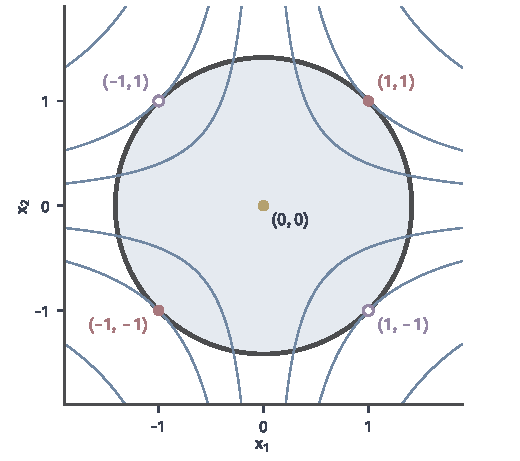
\includegraphics[width=88mm]{figures/05-optimization/06-constrained-optimization/matplotlib/kkt-full-example/figure.pdf}
  \caption{问题~\eqref{eq:kkt-full-example}的候选点。浅蓝圆盘是可行集，蓝线是$-x_1x_2$的等高线。红点$\pm(1,1)$是全局最小点。黄点$(0,0)$是KKT点，但二阶必要条件不成立。紫色空心点$\pm(1,-1)$满足驻定和活动条件，乘子为$-1/2$，不是KKT点。}
  \label{fig:kkt-full-example}
\end{BookInlineFigure}

\section{本章小结}
\label{sec:kkt-summary}

本章回答的问题是：给定一个候选点，怎样只用它附近的信息判断它是否最优。答案不是一个公式，而是按顺序做的几项检查，每一项给出的结论强弱不同，见图~\ref{fig:kkt-decision-flow}。

\begin{BookInlineFigure}
  \centering
  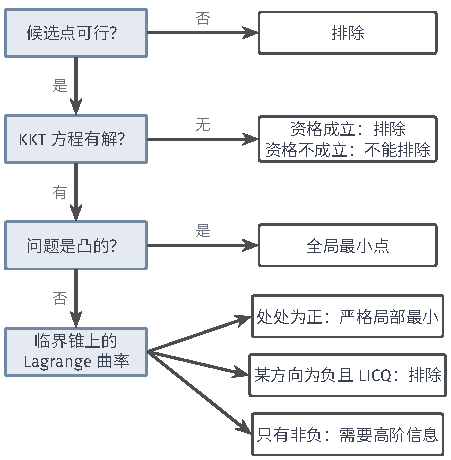
\includegraphics[width=76.3mm]{figures/05-optimization/06-constrained-optimization/tikz/kkt-decision-flow/figure.pdf}
  \caption{判断候选点的流程。左列依次是可行性、KKT方程、凸性和临界锥上的曲率四项检查，右列是对应的结论。“资格”指候选点满足的约束资格，如LICQ或MFCQ。}
  \label{fig:kkt-decision-flow}
\end{BookInlineFigure}

第一项检查是可行性，并找出活动约束。不活动的约束在局部不起作用，所以后面的条件只看活动约束和等式约束。

第二项检查是真实的局部方向。切锥只依赖可行集，它给出最根本的必要条件：局部最小点处，切锥中没有一阶下降方向。线性化锥好算，但可能多出虚假方向。LICQ和MFCQ保证两者相等，这两个条件只涉及约束函数在该点的梯度，与目标的凸性无关，并且会随约束的写法改变。

第三项检查是KKT条件。Farkas引理把“线性化锥中没有下降方向”换成负梯度属于活动梯度的非负锥，由此得到驻定、原始可行、乘子非负和互补松弛四组条件。在MFCQ下它们是局部最小点的必要条件，LICQ进一步保证乘子唯一。没有约束资格时，最小点可以没有乘子。

局部结论和全局结论要分开。目标和不等式约束函数凸、等式约束仿射时，任何KKT点都是全局最小点，这不需要约束资格。一般非凸问题中，KKT点只是候选，全局结论要靠存在性和枚举等其他依据。

第四项检查是曲率。只有一阶变化为零的方向才需要二阶判断，这些方向组成临界锥，零乘子的活动约束在其中保留单侧限制。约束的弯曲通过乘子进入Lagrange函数的Hessian，所以检查的是Lagrange Hessian在临界锥上的二次型，不是目标Hessian，也不是全空间的正定性。LICQ下二次型非负是必要条件；在某组KKT乘子下对非零临界方向严格为正是充分条件，并且给出局部二次增长，这一方向不需要约束资格。两者之间的退化情形，二阶信息判断不了。

这些条件都在已知候选点时做判断，没有回答候选点从哪里来。下一章用乘子构造整个问题的下界，把这里局部的条件变成可以检验的全局证书。可行迭代、乘子更新和局部子问题怎样产生满足这些条件的点，由第~\ref{chap:feasible-iterations}章至第~\ref{chap:nonlinear-interior-point}章研究。


\chapter{对偶问题}
\label{chap:duality}

求解约束问题时，算法交出一个可行点，目标值是$0.40625$。这个数够好吗？可行点本身只说明最优值不超过$0.40625$，至于离最优值还差多少，它什么也没有说。第~\ref{chap:constrained-optimality}章的KKT条件能判断一个候选是否满足最优点应有的关系，却不能给一个非最优的候选打分。要回答“还差多少”，必须另有一个不超过最优值的数，也就是下界。

第~\ref{chap:linear-programming}章已经见过这样的下界：把约束乘上权重加起来，得到一份能当场核对的证据。本章把这个办法推广到一般的约束问题。目标和约束不再是线性的，加权之后也就不能靠比较系数得出下界，而要对原变量取一次下确界。

第~\ref{sec:dual-lower-bound}节构造下界，第~\ref{sec:dual-weak}节说明它为什么总是成立，以及怎样用它给可行点估计误差。下确界的计算反复出现“函数加线性项”的结构，第~\ref{sec:dual-conjugate}节把这个结构提取出来，得到计算对偶问题的工具。

最好的下界未必等于最优值。第~\ref{sec:dual-strong}节研究两者何时相等，并把“相等”“原始最优点存在”“最优乘子存在”这三件事分开。第~\ref{sec:dual-certificates}节把上下界、KKT条件和鞍点放到同一对原始—对偶候选上比较，说明它们各自检验了什么。

\section{下界的构造}
\label{sec:dual-lower-bound}

对一般的约束问题，怎样写出一个不依赖未知最优点的下界？全章讨论的问题是
\begin{equation}
 \begin{aligned}
 \min_{\bm{x}\in\bm{D}}\quad & f(\bm{x})\\
 \text{s.t.}\quad & g_i(\bm{x})\leq0,\quad i=1,\ldots,m,\\
 & h_j(\bm{x})=0,\quad j=1,\ldots,p.
 \end{aligned}
 \label{eq:dual-primal}
\end{equation}
这里$\bm{D}\subseteq\mathbb{R}^n$是规定的定义域，$f,g_i,h_j$在其上都取有限值。没有特别说明时$\bm{D}=\mathbb{R}^n$；有些问题只在一部分点上有定义，或者我们有意把一些简单约束（例如$\bm{x}\geq\bm{0}$）留在$\bm{D}$里。

式~\eqref{eq:dual-primal}称为原始问题，它的最优值记为$f^\star$，是可行点上目标值的下确界。没有可行点时规定$f^\star=+\infty$。我们不假设最小点存在，也不假设问题是凸的，这两点在后面都很重要。

第~\ref{chap:constrained-optimality}章为这个问题定义了Lagrange函数，给每条不等式配乘子$\lambda_i$，每条等式配乘子$\nu_j$：
\begin{equation}
 \mathcal{L}(\bm{x},\bm{\lambda},\bm{\nu})=f(\bm{x})+\sum_{i=1}^m\lambda_ig_i(\bm{x})+\sum_{j=1}^p\nu_jh_j(\bm{x}).
 \label{eq:dual-lagrangian}
\end{equation}
那里用它写出候选点上的驻定条件，这里换一个用法：把它当成原目标的一个替身。

\paragraph{用线性价格代替无穷的墙}
约束可以看成目标里的一堵墙。令$\iota_{\leq0}(u)$在$u\leq0$时为$0$，在$u>0$时为$+\infty$，则不等式约束等价于在目标上加$\iota_{\leq0}(g_i(\bm{x}))$。这个函数太硬，无法与目标一起处理。

换成一条斜率$\lambda\geq0$的直线$\lambda u$。图~\ref{fig:dual-wall-price}(a)显示，不论$\lambda$取多少，直线都在墙的下方：$u\leq0$时$\lambda u\leq0$，$u>0$时墙是$+\infty$。用直线替换墙，得到的函数不会超过原来带墙的目标。

这正是价格的想法。约束超支一单位就付$\lambda$的罚款，有结余就按同样的价格退款，违反约束不再被禁止，只是要付钱。等式约束的乘子$\nu_j$没有符号限制，因为$h_j=0$时无论乘什么数，这一项都为零。这个类比只帮助记住不等式的方向，并不表示真的存在这样的市场。

下面用一个能画出来的例子走一遍，全章称它为\emph{一元例}：
\begin{equation}
 \min_{x\in\mathbb{R}}\ \frac12(x-2)^2\quad\text{s.t.}\quad x-1\leq0.
 \label{eq:dual-oned}
\end{equation}
无约束最小点$x=2$不可行，所以解在边界$x^\star=1$上，最优值$f^\star=1/2$。

取$\lambda=1/2$，Lagrange函数是
\[
 \mathcal{L}(x,\tfrac12)=\frac12(x-2)^2+\frac12(x-1).
\]
在可行点$x\leq1$上，第二项不大于零，所以$\mathcal{L}(x,\frac12)\leq f(x)$。图~\ref{fig:dual-wall-price}(b)中，紫色曲线在阴影区都位于蓝色曲线下方，并且全部经过$(1,\frac12)$，因为那里约束的值恰好为零。

对$x$求最小，驻点满足$x-2+\frac12=0$，即$x=\frac32$，最小值是
\[
 \mathcal{L}(\tfrac32,\tfrac12)=\frac18+\frac14=\frac38.
\]
这个最小点并不可行，这没有关系。它是$\mathcal{L}$在整条数轴上的最小值，当然不超过$\mathcal{L}$在可行点上的值，而后者又不超过$f$。于是我们没有用到$x^\star$，就知道$f^\star\geq3/8$。

\begin{BookInlineFigure}
 \centering
 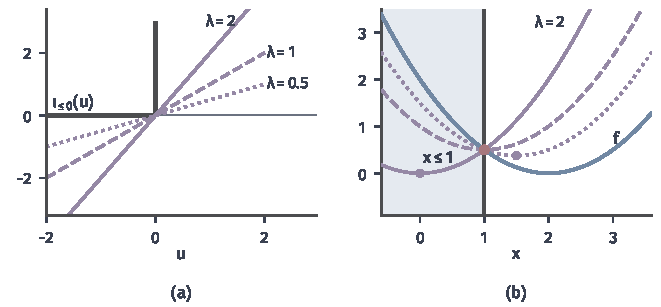
\includegraphics[width=112mm]{figures/05-optimization/06-constrained-optimization/matplotlib/dual-wall-price/figure.pdf}
 \caption{用线性价格代替硬约束。(a)~深灰粗线是硬约束$\iota_{\leq0}(u)$，紫线是$\lambda u$，点线、虚线、实线分别对应$\lambda=0.5,1,2$，都在粗线下方。(b)~一元例~\eqref{eq:dual-oned}：蓝线是目标$f$，浅蓝区域是可行集$x\leq1$，紫线是$\mathcal{L}(\cdot,\lambda)$，线型含义同(a)；紫点是各自的最小点，红点是原始最优点。}
 \label{fig:dual-wall-price}
\end{BookInlineFigure}

这段推理里最容易出错的一步，是必须对$\bm{D}$上的\emph{全部}点取下确界。只求一个驻点是不够的。在$\bm{D}=[-3,3]$上考虑$f(x)=x^3-3x$，约束$x-2\leq0$，取$\lambda=0$，则$\mathcal{L}=f$。驻点$x=1$是局部极小点，值为$-2$，但可行点$x=-3$的目标值是$-18$。局部极小值$-2$不是下界。

\subsection{对偶函数}
\label{sec:dual-function}

把上面的做法写成定义。固定乘子以后，对原变量取下确界，得到的数只依赖乘子。

\begin{definition}[对偶函数]
 \label{def:dual-function}
 问题~\eqref{eq:dual-primal}的\term{对偶函数}（dual function）是
 \begin{equation}
  q(\bm{\lambda},\bm{\nu})=\inf_{\bm{x}\in\bm{D}}\mathcal{L}(\bm{x},\bm{\lambda},\bm{\nu}),
  \label{eq:dual-function}
 \end{equation}
 允许取$-\infty$。使$q$取有限值的乘子组成它的有效定义域$\operatorname{dom}q$。满足$\bm{\lambda}\geq\bm{0}$且$(\bm{\lambda},\bm{\nu})\in\operatorname{dom}q$的乘子称为对偶可行的乘子。
\end{definition}

注意下确界有三种可能，定义中用$\inf$而不是$\min$，正是为了把它们都包括进去。第一种是最小点存在，例如一元例。第二种是下确界为$-\infty$：在$\mathbb{R}$上最小化$-x^2$，约束写成$x-1\leq0$和$-x-1\leq0$，则$\mathcal{L}$对任何乘子都是开口向下的二次函数，$q\equiv-\infty$。这时对偶函数没有提供信息。

第三种是下确界有限但取不到。考虑$\min e^{-x}$，约束$-x\leq0$。取$\lambda=0$，则
\[
 q(0)=\inf_{x\in\mathbb{R}}e^{-x}=0,
\]
这个值没有任何$x$能达到。而$\lambda>0$时，$e^{-x}-\lambda x$在$x\to+\infty$时趋于$-\infty$，所以$q(\lambda)=-\infty$。

现在用第~\ref{chap:constrained-optimality}章的等式二次例计算一个完整的对偶函数，全章称它为\emph{二次例}：
\begin{equation}
 \min_{\bm{x}\in\mathbb{R}^2}\ \frac12(x_1^2+4x_2^2)\quad\text{s.t.}\quad x_1+x_2-1=0.
 \label{eq:dual-quad}
\end{equation}
那里已经由切向导数为零求出最小点$(4/5,1/5)$，最优值是
\[
 f^\star=\frac12\Bigl(\frac{16}{25}+\frac{4}{25}\Bigr)=\frac25.
\]

下面不用这个答案，只用对偶函数。Lagrange函数是
\[
 \mathcal{L}(\bm{x},\nu)=\frac12(x_1^2+4x_2^2)+\nu(x_1+x_2-1).
\]
固定$\nu$，它是$\bm{x}$的严格凸二次函数，令梯度为零就得到唯一的全局最小点：
\[
 x_1+\nu=0,\qquad 4x_2+\nu=0.
\]
因此
\[
 x_1(\nu)=-\nu,\qquad x_2(\nu)=-\frac{\nu}{4}.
\]

代回$\mathcal{L}$，两个平方项和约束项分别是
\[
 \frac12\Bigl(\nu^2+\frac{\nu^2}{4}\Bigr)=\frac58\nu^2,\qquad
 \nu\Bigl(-\nu-\frac{\nu}{4}-1\Bigr)=-\frac54\nu^2-\nu.
\]
相加得到关于$\nu$的一元函数
\begin{equation}
 q(\nu)=-\frac58\nu^2-\nu.
 \label{eq:dual-quad-q}
\end{equation}

这是一条开口向下的抛物线。令导数$-\frac54\nu-1=0$，得到
\[
 \nu^\star=-\frac45,\qquad q(\nu^\star)=-\frac25+\frac45=\frac25.
\]
最好的下界恰好等于$f^\star=2/5$，同时$\bm{x}(\nu^\star)=(4/5,1/5)$也正是原问题的解。

图~\ref{fig:dual-equality-q}(a)显示了这个过程。$\nu$的作用是在目标上加一个倾斜的线性项，把碗底从原点沿紫色虚线推走。$\nu=0$时碗底在原点，不满足约束；$\nu=-4/5$时碗底恰好落到约束直线上。图~\ref{fig:dual-equality-q}(b)是这个过程中碗底的高度随$\nu$的变化，也就是$q(\nu)$。

\begin{BookInlineFigure}
 \centering
 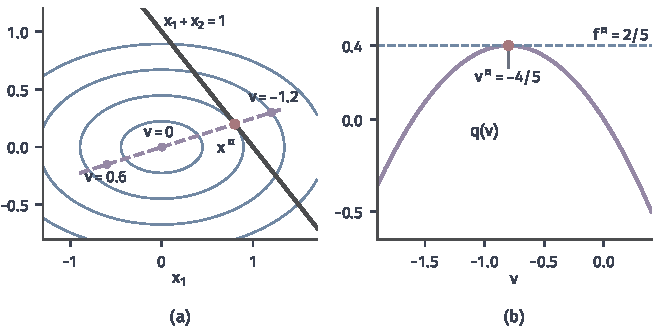
\includegraphics[width=112mm]{figures/05-optimization/06-constrained-optimization/matplotlib/dual-equality-q/figure.pdf}
 \caption{二次例~\eqref{eq:dual-quad}的对偶函数。(a)~蓝线是目标的等高线，深灰粗线是约束$x_1+x_2=1$，紫色虚线是内层最小点$\bm{x}(\nu)=(-\nu,-\nu/4)$的轨迹，红点是$\bm{x}^\star$。(b)~紫线是$q(\nu)$，它处处不超过蓝色虚线$f^\star$，在$\nu^\star=-4/5$处相等。}
 \label{fig:dual-equality-q}
\end{BookInlineFigure}

不等式约束的对偶函数要多处理一件事：内层的$\bm{D}$可以有边界，最小点会在边界上换挡。第~\ref{chap:constrained-optimality}章的预算例取$\tau=2$，就是这种情形，全章称它为\emph{预算例}：
\begin{equation}
 \min_{\bm{x}\geq\bm{0}}\ \frac12\bigl[(x_1-2)^2+(x_2-1)^2\bigr]\quad\text{s.t.}\quad x_1+x_2-2\leq0.
 \label{eq:dual-budget}
\end{equation}
把$\bm{x}\geq\bm{0}$留在$\bm{D}=\mathbb{R}^2_{+}$中，只给预算约束配乘子$\lambda\geq0$。

此时内层问题按坐标分开：
\[
 \min_{x_1\geq0}\Bigl[\frac12(x_1-2)^2+\lambda x_1\Bigr]+\min_{x_2\geq0}\Bigl[\frac12(x_2-1)^2+\lambda x_2\Bigr]-2\lambda.
\]
每一项是开口向上的一元二次函数在半轴上的最小化，最小点是无约束最小点截断到非负：
\[
 x_1(\lambda)=\max\{2-\lambda,0\},\qquad x_2(\lambda)=\max\{1-\lambda,0\}.
\]

$\lambda$越过$1$时第二个坐标碰到边界，越过$2$时第一个坐标也碰到边界。分三段代入，得到
\begin{equation}
 q(\lambda)=\begin{cases}
 \lambda-\lambda^2, & 0\leq\lambda\leq1,\\
 \dfrac12-\dfrac12\lambda^2, & 1\leq\lambda\leq2,\\
 \dfrac52-2\lambda, & \lambda\geq2.
 \end{cases}
 \label{eq:dual-budget-q}
\end{equation}

三段在分界点连续：$\lambda=1$时都是$0$，$\lambda=2$时都是$-3/2$。第一段的最大点是$\lambda^\star=1/2$，最好的下界是$q(1/2)=1/4$。

这个例子的解是$\bm{x}^\star=(3/2,1/2)$，目标值$\frac12(\frac14+\frac14)=\frac14$，下界再次与最优值相等。图~\ref{fig:dual-budget-q}中，内层最小点随$\lambda$增大沿折线向原点移动，价格越高，用得越少；$q$相应地分成三段。

\begin{BookInlineFigure}
 \centering
 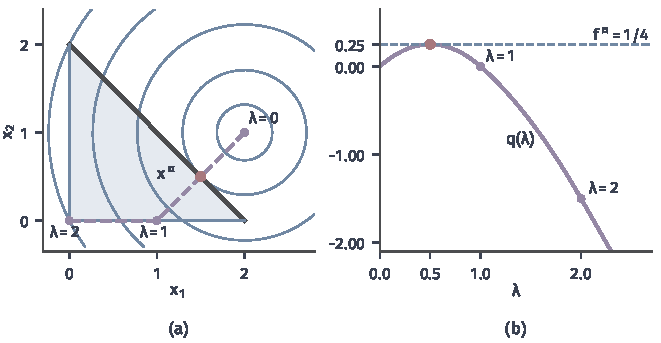
\includegraphics[width=112mm]{figures/05-optimization/06-constrained-optimization/matplotlib/dual-budget-q/figure.pdf}
 \caption{预算例~\eqref{eq:dual-budget}的对偶函数。(a)~浅蓝区域是可行集，深灰粗线是预算约束，蓝线是目标等高线，紫色虚线是内层最小点$\bm{x}(\lambda)$随$\lambda$从$0$增大的轨迹，紫点是$\lambda=0,1,2$时的位置，红点是$\bm{x}^\star$。(b)~紫线是分段的$q(\lambda)$，紫点是分界点，红点是最大点$(1/2,1/4)$。}
 \label{fig:dual-budget-q}
\end{BookInlineFigure}

\subsection{对偶问题}
\label{sec:dual-problem}

每组合法的乘子给出一个下界，下界越大提供的信息越多。很自然地，我们想要最大的那个，于是得到一个新的优化问题。

\begin{definition}[对偶问题]
 \label{def:dual-problem}
 问题~\eqref{eq:dual-primal}的对偶问题是在合法乘子上最大化对偶函数，
 \begin{equation}
  d^\star=\sup_{\bm{\lambda}\geq\bm{0},\ \bm{\nu}}q(\bm{\lambda},\bm{\nu}),
  \label{eq:dual-problem}
 \end{equation}
 其最优值$d^\star$可以取$\pm\infty$；对偶可行的乘子不存在时$d^\star=-\infty$。达到这个上确界的乘子称为对偶最优乘子。
\end{definition}

这里的约束只有$\bm{\lambda}\geq\bm{0}$，比原问题简单。更值得注意的是目标函数的形状。图~\ref{fig:dual-budget-q}(b)和图~\ref{fig:dual-equality-q}(b)中的$q$都是凹的，这不是巧合。

要看出原因，把$\mathcal{L}$反过来读：固定$\bm{x}$，它关于乘子是仿射函数，斜率是约束值$g_i(\bm{x})$与$h_j(\bm{x})$，截距是$f(\bm{x})$。$q$是这一族直线的下包络。图~\ref{fig:dual-affine-envelope}中一元例的每条直线对应一个$x$，它们的下包络（紫线）向下弯曲。

\begin{theorem}[对偶函数是凹的]
 \label{thm:dual-concave}
 对问题~\eqref{eq:dual-primal}，无论$f,g_i,h_j$和$\bm{D}$是否凸，$q$都是凹函数，$\operatorname{dom}q$是凸集。
\end{theorem}

\begin{proof}
 记$\bm{a}=(\bm{\lambda},\bm{\nu})$。任取$\bm{a}_1,\bm{a}_2$和$\theta\in[0,1]$，令$\bm{a}=\theta\bm{a}_1+(1-\theta)\bm{a}_2$。$\mathcal{L}$对乘子是仿射的，所以对每个$\bm{x}\in\bm{D}$，
 \[
  \mathcal{L}(\bm{x},\bm{a})=\theta\mathcal{L}(\bm{x},\bm{a}_1)+(1-\theta)\mathcal{L}(\bm{x},\bm{a}_2).
 \]
 由下确界的定义，右端不小于$\theta q(\bm{a}_1)+(1-\theta)q(\bm{a}_2)$。对$\bm{x}\in\bm{D}$取下确界，得到
 \[
  q(\bm{a})\geq\theta q(\bm{a}_1)+(1-\theta)q(\bm{a}_2).
 \]
 若$\bm{a}_1,\bm{a}_2\in\operatorname{dom}q$，右端有限，于是$\bm{a}\in\operatorname{dom}q$。
\end{proof}

\begin{BookInlineFigure}
 \centering
 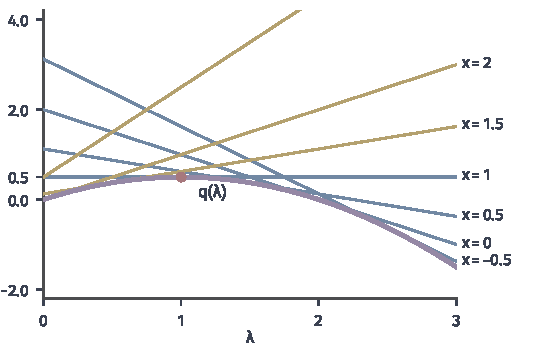
\includegraphics[width=92mm]{figures/05-optimization/06-constrained-optimization/matplotlib/dual-affine-envelope/figure.pdf}
 \caption{一元例中，每个固定的$x$给出一条直线$\lambda\mapsto\mathcal{L}(x,\lambda)$，蓝线对应可行的$x$，黄线对应不可行的$x$（最陡的一条是$x=3$），紫线是下包络$q(\lambda)=\lambda-\lambda^2/2$。可行点的直线斜率不为正，所以在$\lambda\geq0$上不超过其截距$f(x)$；水平粗线是$x=1$，高度为$f^\star=1/2$，在红点处与$q$相切。}
 \label{fig:dual-affine-envelope}
\end{BookInlineFigure}

定理~\ref{thm:dual-concave}说的是一个凸优化问题总摆在手边，无论原问题多么复杂，最大化一个凹函数原则上没有多余的局部最优。但这并不意味着对偶问题容易求解。计算$q$的一个值就要做一次内层的全局最小化，而内层目标$\mathcal{L}(\cdot,\bm{\lambda},\bm{\nu})$可以和原目标一样非凸。前面$f(x)=x^3-3x$的例子说明，局部解在这里给不出下界。凹性属于外层，难度可能全部留在内层。

线性规划是内层可以完全算出的特例。把第~\ref{chap:linear-programming}章的标准型$\min\bm{c}^\top\bm{x}$，$\bm{A}\bm{x}=\bm{b}$，$\bm{x}\geq\bm{0}$放进这个框架，取$\bm{D}=\mathbb{R}^n$。给不等式$-\bm{x}\leq\bm{0}$配乘子$\bm{s}\geq\bm{0}$，给等式配乘子$-\bm{y}$，则
\[
 \mathcal{L}=\bm{c}^\top\bm{x}-\bm{y}^\top(\bm{A}\bm{x}-\bm{b})-\bm{s}^\top\bm{x}=\bm{b}^\top\bm{y}+(\bm{c}-\bm{A}^\top\bm{y}-\bm{s})^\top\bm{x}.
\]

这是$\bm{x}$的线性函数，只有斜率为零时下确界才有限：
\[
 q(\bm{s},\bm{y})=\begin{cases}\bm{b}^\top\bm{y}, & \bm{A}^\top\bm{y}+\bm{s}=\bm{c},\\ -\infty, & \text{其他情形}.\end{cases}
\]
第~\ref{chap:linear-programming}章对偶问题的等式约束$\bm{A}^\top\bm{y}+\bm{s}=\bm{c}$，在这里的含义是$\operatorname{dom}q$的条件。把$q=-\infty$的乘子排除后，再最大化$\bm{b}^\top\bm{y}$，就回到了那里的对偶问题。

\section{弱对偶}
\label{sec:dual-weak}

上一节在例子里反复看到“下界不超过最优值”。这个结论在什么范围内成立，它又能为手里的候选点提供什么？

\begin{theorem}[弱对偶]
 \label{thm:dual-weak}
 对问题~\eqref{eq:dual-primal}的任一可行点$\bm{x}$和任一组$\bm{\lambda}\geq\bm{0}$、$\bm{\nu}$，有
 \begin{equation}
  q(\bm{\lambda},\bm{\nu})\leq f(\bm{x}).
  \label{eq:dual-weak-pair}
 \end{equation}
 因而
 \begin{equation}
  d^\star\leq f^\star.
  \label{eq:dual-weak}
 \end{equation}
\end{theorem}

\begin{proof}
 由可行性和$\bm{\lambda}\geq\bm{0}$，有$\lambda_ig_i(\bm{x})\leq0$和$\nu_jh_j(\bm{x})=0$，所以这些项都不使$f(\bm{x})$增大。又因为$\bm{x}\in\bm{D}$，由下确界的定义，
 \[
  q(\bm{\lambda},\bm{\nu})\leq\mathcal{L}(\bm{x},\bm{\lambda},\bm{\nu})\leq f(\bm{x}).
 \]
 左边不含$\bm{x}$，对可行点取下确界，再对合法乘子取上确界，就得到式~\eqref{eq:dual-weak}。没有可行点时$f^\star=+\infty$，式~\eqref{eq:dual-weak}自然成立。
\end{proof}

证明只用了两件事：下确界的定义，以及符号。它不需要凸性，不需要可微性，也不需要任何约束资格。正因为条件这样少，弱对偶可以用于任何问题，这是它最大的价值。

\term{弱对偶}这个名字在第~\ref{chap:linear-programming}章已经出现过，那里说的是线性规划的特例。两个差要分清。一个是某一对候选的差$f(\bm{x})-q(\bm{\lambda},\bm{\nu})$，下面称为\emph{候选间隙}，算法每一步都能算出。另一个是两个最优值的差$f^\star-d^\star$，这是问题本身的性质，称为\term{对偶间隙}。候选间隙总不小于对偶间隙。

\paragraph{在目标—约束平面上看弱对偶}
把每个$x$映成平面上的一点$(u,t)=(g(x),f(x))$，横坐标是约束值，纵坐标是目标值，这些点组成集合$\bm{G}$。对一元例，$u=x-1$，$t=\frac12(u-1)^2$，$\bm{G}$是一条抛物线，如图~\ref{fig:dual-image-set}所示。可行点对应$u\leq0$，原始问题就是在竖线左侧找$\bm{G}$的最低点。

$\mathcal{L}=t+\lambda u$在斜率为$-\lambda$的直线上为常数。$q(\lambda)$就是把这样的直线从下方推到刚好碰到$\bm{G}$，这条直线与竖轴$u=0$的交点高度。

所以弱对偶的几何含义是：直线在$\bm{G}$下方，$\lambda\geq0$时它在$u\leq0$一侧向左不下降，因此$\bm{G}$中$u\leq0$的部分都在交点上方。对偶问题就是转动直线，使交点尽量高。$\lambda$取负数时直线向左下降，交点就可能高过可行部分的最低点，后面会看到这个现象。

\begin{BookInlineFigure}
 \centering
 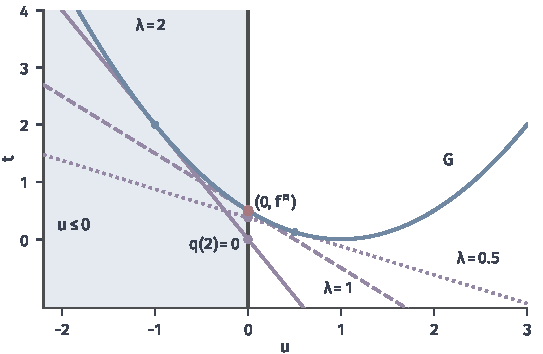
\includegraphics[width=92mm]{figures/05-optimization/06-constrained-optimization/matplotlib/dual-image-set/figure.pdf}
 \caption{一元例在$(u,t)=(g(x),f(x))$平面上的像。蓝线是$\bm{G}$，浅蓝区域是可行的半平面$u\leq0$，深灰粗线是$u=0$。紫线是斜率$-\lambda$的支撑直线（$\lambda=0.5,1,2$，分别为点线、虚线、实线），它们在$\bm{G}$下方，与$u=0$的交点（紫点）高度就是$q(\lambda)$，分别为$0.375$、$0.5$、$0$。红点$(0,f^\star)$是$\lambda=1$时的切点。}
 \label{fig:dual-image-set}
\end{BookInlineFigure}

\subsection{可行候选的误差证书}
\label{sec:dual-certificate}

现在回答本章开头的问题。手里有一个可行点$\hat{\bm{x}}$和一组合法乘子$(\bm{\lambda},\bm{\nu})$，由弱对偶，最优值被夹在两个可计算的数之间：
\begin{equation}
 q(\bm{\lambda},\bm{\nu})\leq f^\star\leq f(\hat{\bm{x}}).
 \label{eq:dual-sandwich}
\end{equation}
两边同时减去，得到次优性的一个可以计算的上界：
\begin{equation}
 0\leq f(\hat{\bm{x}})-f^\star\leq f(\hat{\bm{x}})-q(\bm{\lambda},\bm{\nu}).
 \label{eq:dual-gap-certificate}
\end{equation}
右端不含$f^\star$，这一对候选本身就是一份\emph{误差证书}。第~\ref{chap:optimization}章讨论过目标差难以计算的困难，这里给出了一种解决办法。

用二次例算一组不是最优的候选。取可行点和乘子
\[
 \hat{\bm{x}}=\Bigl(\frac34,\frac14\Bigr),\qquad\nu=-\frac34.
\]
原始目标值由定义计算，对偶目标值由式~\eqref{eq:dual-quad-q}计算：
\[
 f(\hat{\bm{x}})=\frac12\Bigl(\frac{9}{16}+\frac{4}{16}\Bigr)=\frac{13}{32},\qquad
 q\Bigl(-\frac34\Bigr)=-\frac{45}{128}+\frac34=\frac{51}{128}.
\]

候选间隙是
\[
 \frac{13}{32}-\frac{51}{128}=\frac{52-51}{128}=\frac{1}{128}\approx0.0078.
\]
所以不用知道答案，我们就确认$\hat{\bm{x}}$的目标差不超过$0.0078$。

因为这个例子知道答案，可以核对证书有多紧。真实目标差和乘子一侧的差分别是
\[
 \frac{13}{32}-\frac25=\frac{1}{160},\qquad\frac25-\frac{51}{128}=\frac{1}{640}.
\]
两者之和是
\[
 \frac{1}{160}+\frac{1}{640}=\frac{5}{640}=\frac{1}{128},
\]
正是候选间隙。候选间隙同时度量了原始和对偶两侧的误差，图~\ref{fig:dual-certificate-line}把这几个数放在同一条数轴上。

\begin{BookInlineFigure}
 \centering
 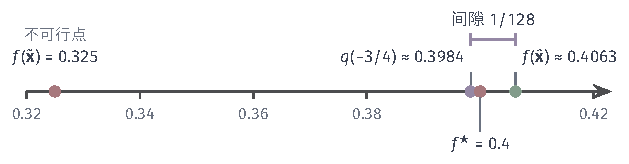
\includegraphics[width=106.4mm]{figures/05-optimization/06-constrained-optimization/tikz/dual-certificate-line/figure.pdf}
 \caption{二次例的误差证书。紫点是下界$q(-3/4)$，绿点是可行点$\hat{\bm{x}}$的目标值，红点$f^\star$夹在两者之间，紫色括线是候选间隙。左边的红点是不可行点$\tilde{\bm{x}}=(0.7,0.2)$的目标值，它比$f^\star$低，不能用来估计误差。}
 \label{fig:dual-certificate-line}
\end{BookInlineFigure}

式~\eqref{eq:dual-gap-certificate}有三个前提，每一个都要单独检验，下面逐一看缺了会怎样。

第一个是原始可行性。点$\tilde{\bm{x}}=(0.7,0.2)$不满足约束，因为$0.7+0.2\neq1$。它的目标值只有
\[
 f(\tilde{\bm{x}})=\frac12(0.49+0.16)=0.325,
\]
比最优值低，与下界的差是$0.325-0.3984\approx-0.073$，是负数。负的“间隙”在这里暴露了不可行，但一般不能指望这样：不可行点也可能给出正的小间隙。所以约束残差要另外计算，不能从间隙看出来。

第二个是乘子的合法性。考虑$\min x^2$，约束$x-1\leq0$，最优值$f^\star=0$。内层最小点是$x=-\lambda/2$，代回得到
\[
 q(\lambda)=-\frac{\lambda^2}{4}-\lambda.
\]
这个公式对负的$\lambda$照样能算，例如$\lambda=-2$时给出$q=1$，比真实最优值$0$还大。

错在哪里？$\lambda=-2$时，可行点$x=0$上的$\mathcal{L}=0-2(0-1)=2$，比$f(0)=0$大，证明中$\mathcal{L}\leq f$这一步失效。图~\ref{fig:dual-illegal-multiplier}中红色虚线高过了$f^\star$，这段就是不合法的乘子。

\begin{BookInlineFigure}
 \centering
 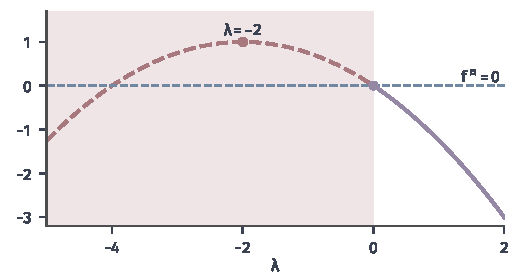
\includegraphics[width=88mm]{figures/05-optimization/06-constrained-optimization/matplotlib/dual-illegal-multiplier/figure.pdf}
 \caption{乘子合法性的作用。问题是$\min x^2$，约束$x-1\leq0$。紫线是$\lambda\geq0$时的$q(\lambda)$，始终不超过蓝色虚线$f^\star=0$；红色虚线和浅红区域对应$\lambda<0$，同一个公式在这里可以超过$f^\star$，例如$\lambda=-2$时为$1$，它不是下界。}
 \label{fig:dual-illegal-multiplier}
\end{BookInlineFigure}

第三个前提是下界本身算得可信，也就是内层下确界确实是下确界。这一点在实际计算中最容易被忽略，单独放在下一小节讨论。

\subsection{内层近似的方向}
\label{sec:dual-inexact-inner}

计算$q$需要解一个最小化问题。多数情况下内层得不到解析解，只能迭代到某个近似点$\tilde{\bm{x}}$。这样算出的$\mathcal{L}(\tilde{\bm{x}},\bm{\lambda},\bm{\nu})$可不可以当作下界使用？

答案是不可以，而且误差的方向恰好不对。由下确界的定义，
\[
 \mathcal{L}(\tilde{\bm{x}},\bm{\lambda},\bm{\nu})\geq q(\bm{\lambda},\bm{\nu}),
\]
近似值落在真正下界的\emph{上方}。普通的数值误差只让答案不够精确，这里的误差却可能让“下界”超过最优值，于是证书本身失效。

还是看二次例，固定$\nu=-3/4$。精确的内层解是$\bm{x}(\nu)=(3/4,3/16)$。假设迭代停在
\[
 \tilde{\bm{x}}=(0.8,0.15).
\]
此处的Lagrange函数值是
\[
 \mathcal{L}(\tilde{\bm{x}},\nu)=\frac12(0.64+0.09)-0.75\,(0.8+0.15-1)=0.365+0.0375=0.4025.
\]
这个数比$f^\star=0.4$还大。如果把它当作下界，就会得出一个错误的结论，以为最优值不小于$0.4025$。

要得到可靠的下界，必须从近似值中扣除一个经过证明的量。若内层函数有已知的曲率下界，用梯度残差就可以写出这个量。

\begin{lemma}[由梯度残差得到的认证下界]
 \label{lem:dual-certified-bound}
 设$\bm{D}=\mathbb{R}^n$，$\bm{\lambda}\geq\bm{0}$，函数$\mathcal{L}(\cdot,\bm{\lambda},\bm{\nu})$可微且是$\mu$强凸的，$\mu>0$。则对任意$\tilde{\bm{x}}$，
 \begin{equation}
  q(\bm{\lambda},\bm{\nu})\geq\mathcal{L}(\tilde{\bm{x}},\bm{\lambda},\bm{\nu})-\frac{1}{2\mu}\bigl\lVert\nabla_{\bm{x}}\mathcal{L}(\tilde{\bm{x}},\bm{\lambda},\bm{\nu})\bigr\rVert_2^2.
  \label{eq:dual-certified-bound}
 \end{equation}
\end{lemma}

\begin{proof}
 记$\phi=\mathcal{L}(\cdot,\bm{\lambda},\bm{\nu})$，$\bm{r}=\nabla\phi(\tilde{\bm{x}})$。由$\mu$强凸的一阶不等式，对任意$\bm{y}$，
 \[
  \phi(\bm{y})\geq\phi(\tilde{\bm{x}})+\langle\bm{r},\bm{y}-\tilde{\bm{x}}\rangle+\frac{\mu}{2}\lVert\bm{y}-\tilde{\bm{x}}\rVert_2^2.
 \]
 右端是$\bm{y}$的二次函数，在$\bm{y}=\tilde{\bm{x}}-\bm{r}/\mu$处最小，最小值为$\phi(\tilde{\bm{x}})-\lVert\bm{r}\rVert_2^2/(2\mu)$。于是对任意$\bm{y}$，
 \[
  \phi(\bm{y})\geq\phi(\tilde{\bm{x}})-\frac{1}{2\mu}\lVert\bm{r}\rVert_2^2.
 \]
 对$\bm{y}$取下确界即得。
\end{proof}

式~\eqref{eq:dual-certified-bound}的含义是：曲率下界$\mu$限制了函数在$\tilde{\bm{x}}$附近能下降多少，碗不会比它更平，所以梯度残差所能带来的下降有上限，我们把这个上限全部扣掉。

代入例子。Hessian是$\operatorname{diag}(1,4)$，取$\mu=1$。梯度和扣除量分别是
\[
 \nabla_{\bm{x}}\mathcal{L}(\tilde{\bm{x}},\nu)=(x_1+\nu,\,4x_2+\nu)=(0.05,-0.15),\qquad\frac{1}{2\mu}\lVert\cdot\rVert_2^2=\frac{0.025}{2}=0.0125.
\]
认证下界是
\[
 0.4025-0.0125=0.39.
\]

它确实低于真正的$q(-3/4)=0.3984$。图~\ref{fig:dual-inner-approx}把这些数排在一起：未修正的内层值在$f^\star$上方，认证下界在$q$下方。把它和$f(\hat{\bm{x}})=0.40625$配对，得到的候选间隙是$0.01625$，比精确内层的$0.0078$宽，但它是可信的。

\begin{BookInlineFigure}
 \centering
 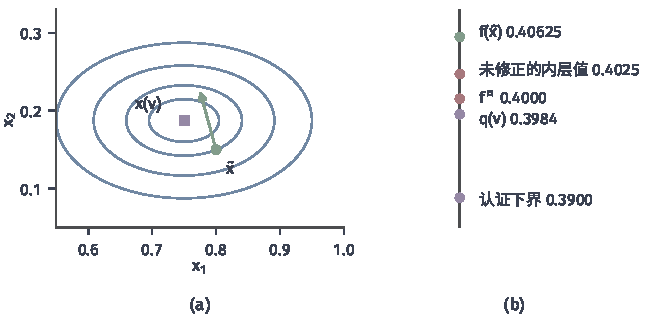
\includegraphics[width=112mm]{figures/05-optimization/06-constrained-optimization/matplotlib/dual-inner-approx/figure.pdf}
 \caption{近似内层的方向。(a)~蓝线是$\mathcal{L}(\cdot,-3/4)$的等高线，紫色方块是精确内层解$\bm{x}(\nu)$，绿点是近似点$\tilde{\bm{x}}$，绿色箭头是负梯度方向。(b)~数轴上由下往上是认证下界、精确的$q(\nu)$、$f^\star$、未修正的内层值和可行点的目标值；未修正的内层值高于$f^\star$，不能当作下界。}
 \label{fig:dual-inner-approx}
\end{BookInlineFigure}

式中的$\mu$必须是真正的曲率下界。若误把$\mathcal{L}$的最大曲率$4$当作$\mu$，扣除量只有$0.025/8=0.003125$，得到$0.399375$，已经超过真正的$q=0.3984$，证书不再成立。当内层没有已知的强凸常数，或者$\bm{D}$不是全空间时，这个引理不能直接使用；此时内层的近似值只能算是一个估计，不能写进误差证书。

\section{凸共轭}
\label{sec:dual-conjugate}

计算对偶函数时，内层总是“目标加上一个线性项，再取下确界”。线性等式约束$\bm{A}\bm{x}=\bm{b}$的对偶函数就是
\[
 q(\bm{\nu})=\inf_{\bm{x}}\bigl\{f(\bm{x})+\langle\bm{A}^\top\bm{\nu},\bm{x}\rangle\bigr\}-\bm{b}^\top\bm{\nu}.
\]
能否把“$f$加线性项后的下确界”事先算好，以后遇到不同的约束时直接取用？这个运算单独拿出来，就是凸共轭。

\subsection{共轭的定义与计算}
\label{sec:dual-conjugate-definition}

下确界$\inf_{\bm{x}}\{f(\bm{x})+\langle\bm{c},\bm{x}\rangle\}$有一个直观的图景。固定斜率$\bm{y}$，拿一把这个斜率的直尺从下方往上顶，顶到碰到$f$为止。这把直尺就是斜率为$\bm{y}$的最高仿射下界。要求直线$\langle\bm{y},\bm{x}\rangle-\beta$处处不超过$f$，等价于对所有$\bm{x}$有
\[
 \beta\geq\langle\bm{y},\bm{x}\rangle-f(\bm{x}).
\]
最小的$\beta$是右端对$\bm{x}$的上确界，这就是下面的定义。

\begin{definition}[凸共轭]
 \label{def:dual-conjugate}
 设$f:\mathbb{R}^n\to\mathbb{R}\cup\{+\infty\}$是适当函数。它的\term{凸共轭}（convex conjugate）是
 \begin{equation}
  f^*(\bm{y})=\sup_{\bm{x}\in\operatorname{dom}f}\bigl\{\langle\bm{y},\bm{x}\rangle-f(\bm{x})\bigr\},
  \label{eq:dual-conjugate}
 \end{equation}
 取值于$\mathbb{R}\cup\{+\infty\}$。
\end{definition}

记号上要小心，$f^*$是共轭函数，$f^\star$是最优值，两者不是一回事。对固定的$\bm{x}$，$\langle\bm{y},\bm{x}\rangle-f(\bm{x})$是$\bm{y}$的仿射函数，$f^*$是它们的上确界，所以无论$f$是否凸，$f^*$总是凸的。这与定理~\ref{thm:dual-concave}是同一个论证。

图~\ref{fig:dual-conj-tangent}(a)取$f(x)=x^2$，斜率$y=2$。过原点的点线$2x$在$x=1$处比$f$高出最多，这个最大的竖直距离是$1$。把点线向下平移$1$，得到切线$2x-1$，它与竖轴的交点是$-f^*(2)$。所以$f^*(y)$是把斜率$y$的直线降到$f$之下需要降多少。

也可以把$\bm{y}$读成价格，把$f(\bm{x})$读成生产$\bm{x}$的成本，于是$f^*(\bm{y})$是价格$\bm{y}$下能得到的最大利润。这个类比说明了为什么$f^*$对$\bm{y}$是凸的：价格上涨时，厂商可以调整产量，利润的增长比线性更快。类比的边界在于$\bm{x}$可以取负值，$f$也不必是真实的成本。

\begin{BookInlineFigure}
 \centering
 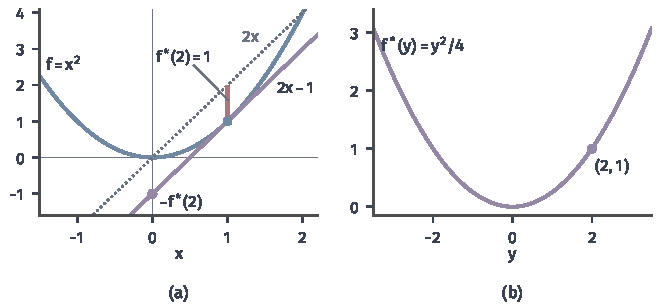
\includegraphics[width=112mm]{figures/05-optimization/06-constrained-optimization/matplotlib/dual-conj-tangent/figure.pdf}
 \caption{共轭是最高仿射下界的截距。(a)~蓝线是$f(x)=x^2$，灰色点线是$y=2$的直线$2x$，红色线段是它与$f$的最大竖直距离$f^*(2)=1$，紫线是下移后的切线，紫点是截距$-f^*(2)$。(b)~紫线是共轭函数$f^*(y)=y^2/4$，紫点对应$y=2$。}
 \label{fig:dual-conj-tangent}
\end{BookInlineFigure}

下面计算三个基本的共轭，每个都要回答一个问题：$f^*$在哪些$\bm{y}$上取有限值。

\paragraph{正定二次函数}
设$\bm{Q}\in\mathbb{R}^{n\times n}$对称正定，$f(\bm{x})=\frac12\bm{x}^\top\bm{Q}\bm{x}$。对$\bm{x}$配方，令$\bm{w}=\bm{x}-\bm{Q}^{-1}\bm{y}$，得到
\[
 \langle\bm{y},\bm{x}\rangle-\frac12\bm{x}^\top\bm{Q}\bm{x}=\frac12\bm{y}^\top\bm{Q}^{-1}\bm{y}-\frac12\bm{w}^\top\bm{Q}\bm{w}.
\]
第二项非正，在$\bm{w}=\bm{0}$时取零，于是
\begin{equation}
 f^*(\bm{y})=\frac12\bm{y}^\top\bm{Q}^{-1}\bm{y}.
 \label{eq:dual-conj-quadratic}
\end{equation}

正定性保证上确界在每个$\bm{y}$上都有限。$f(x)=x^2$相当于$Q=2$，式~\eqref{eq:dual-conj-quadratic}给出$f^*(y)=y^2/4$，$f^*(2)=1$，与图一致。

若$\bm{Q}$只是半正定，$f^*$的有限范围会缩小。例如$\mathbb{R}^2$上的$f(\bm{x})=\frac12x_1^2$，只要$y_2\neq0$，沿$x_2$方向无限走，$\langle\bm{y},\bm{x}\rangle$就趋于$+\infty$，所以$f^*(\bm{y})=+\infty$；只有$y_2=0$时，$f^*(\bm{y})=\frac12y_1^2$。

最极端的情形是线性函数$f(\bm{x})=\langle\bm{a},\bm{x}\rangle$。上确界$\sup_{\bm{x}}\langle\bm{y}-\bm{a},\bm{x}\rangle$只有$\bm{y}=\bm{a}$时有限，此时为$0$。这正是线性规划对偶中出现等式约束的原因。

\paragraph{范数}
设$\lVert\cdot\rVert$是$\mathbb{R}^n$上的一个范数。为了表述结果，先定义它的\term{对偶范数}（dual norm）：
\begin{equation}
 \lVert\bm{y}\rVert_*=\sup_{\lVert\bm{x}\rVert\leq1}\langle\bm{y},\bm{x}\rangle.
 \label{eq:dual-dual-norm}
\end{equation}
由定义，对所有$\bm{x}$，
\[
 \langle\bm{y},\bm{x}\rangle\leq\lVert\bm{y}\rVert_*\lVert\bm{x}\rVert.
\]

现在求$f(\bm{x})=\lVert\bm{x}\rVert$的共轭，分两种情形。若$\lVert\bm{y}\rVert_*\leq1$，由上式，线性项不超过范数，差值不大于零，并在$\bm{x}=\bm{0}$取到零，上确界为$0$。若$\lVert\bm{y}\rVert_*>1$，存在$\lVert\bm{x}_0\rVert\leq1$使$\langle\bm{y},\bm{x}_0\rangle>1$，于是线性项超过范数；沿$s\bm{x}_0$放大，差值随$s$线性增长，趋于$+\infty$。

合起来，范数的共轭是对偶范数单位球的约束指标函数：
\begin{equation}
 f^*(\bm{y})=\iota_{\{\lVert\bm{y}\rVert_*\leq1\}}(\bm{y}).
 \label{eq:dual-conj-norm}
\end{equation}

图~\ref{fig:dual-conj-norm}(a)和(b)是一元情形$f(x)=\lvert x\rvert$。斜率的绝对值不超过$1$的直线都能放在折线下方，斜率$1.5$的直线在$x>0$一侧无论怎样下移，最终都会越过$\lvert x\rvert$。

\paragraph{集合的约束指标函数}
设$\bm{C}$非空。由定义，
\begin{equation}
 \iota_{\bm{C}}^*(\bm{y})=\sup_{\bm{x}\in\bm{C}}\langle\bm{y},\bm{x}\rangle=:\sigma_{\bm{C}}(\bm{y}),
 \label{eq:dual-support}
\end{equation}
$\sigma_{\bm{C}}$称为$\bm{C}$的\term{支撑函数}（support function）。它回答：沿方向$\bm{y}$看，集合最远伸到哪里。集合有界时它处处有限，无界时在某些方向上可能为$+\infty$。

一元的例子是$\bm{C}=[-1,2]$。$y\geq0$时最远点是$2$，$y<0$时最远点是$-1$，所以
\[
 \sigma_{\bm{C}}(y)=\max\{2y,-y\},
\]
这是图~\ref{fig:dual-conj-norm}(c)的折线。

\begin{BookInlineFigure}
 \centering
 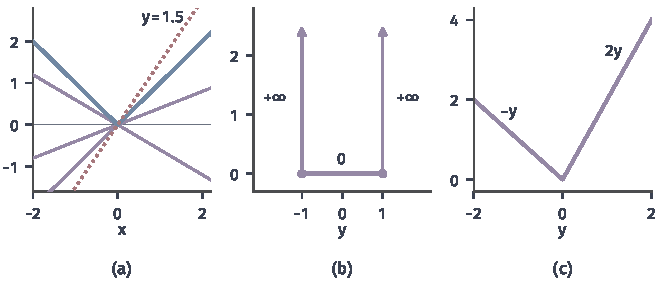
\includegraphics[width=112mm]{figures/05-optimization/06-constrained-optimization/matplotlib/dual-conj-norm/figure.pdf}
 \caption{范数与集合的共轭。(a)~蓝线是$\lvert x\rvert$，紫线是斜率$-0.6,0.4,1$的直线，都在折线下方；红色点线斜率$1.5$，不能下移成下界。(b)~$\lvert x\rvert$的共轭：在$[-1,1]$上为$0$，其余为$+\infty$。(c)~集合$[-1,2]$的支撑函数$\max\{2y,-y\}$。}
 \label{fig:dual-conj-norm}
\end{BookInlineFigure}

二维的例子能同时看到范数和支撑函数的关系。取$\bm{C}$为$\ell_1$单位球，$\bm{y}=(2,1)$。线性函数在多面体上的最大值在顶点取得，比较四个顶点$(\pm1,0),(0,\pm1)$，得到
\[
 \sigma_{\bm{C}}(\bm{y})=\max\{2,-2,1,-1\}=2=\lVert\bm{y}\rVert_\infty.
\]
一般地，$\ell_1$单位球的支撑函数就是$\ell_\infty$范数，也就是说$\ell_1$与$\ell_\infty$互为对偶范数。

图~\ref{fig:dual-support-geometry}(a)中，法向量为$\bm{y}$的直线沿$\bm{y}$方向平移，在$(1,0)$处最后一次碰到菱形。图~\ref{fig:dual-support-geometry}(b)画出了对偶范数的单位球：紫点$(0.6,0.4)$在方块内，线性项处处不超过$\ell_1$范数；红点$(1.4,0.8)$在方块外，取$\bm{x}=(1,0)$，线性项等于$1.4$，超过$\lVert\bm{x}\rVert_1=1$。

\begin{BookInlineFigure}
 \centering
 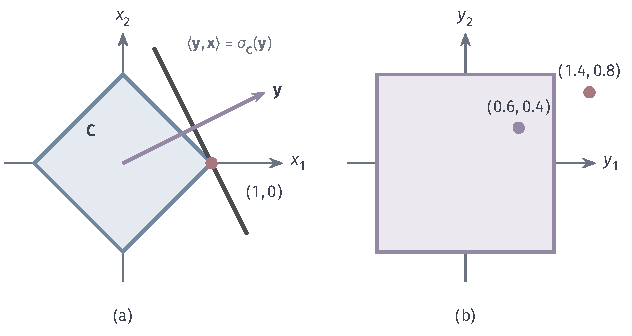
\includegraphics[width=107mm]{figures/05-optimization/06-constrained-optimization/tikz/dual-support-geometry/figure.pdf}
 \caption{支撑函数与对偶范数。(a)~浅蓝菱形是$\ell_1$单位球$\bm{C}$，紫色箭头是方向$\bm{y}=(2,1)$，深灰粗线是在红点$(1,0)$处碰到$\bm{C}$的直线$\langle\bm{y},\bm{x}\rangle=\sigma_{\bm{C}}(\bm{y})=2$。(b)~浅紫方块是$\lVert\bm{y}\rVert_\infty\leq1$，方块内的紫点使共轭为$0$，方块外的红点使共轭为$+\infty$。}
 \label{fig:dual-support-geometry}
\end{BookInlineFigure}

表~\ref{tab:dual-conjugates}汇总了这些结果，并把标量放缩算进去。这些函数常作为作用在辅助变量$\bm{z}$上的惩罚项，所以表中用$\bm{z}$和$\bm{\nu}$作变量。它显示出硬约束与软惩罚在对偶一侧的关系：硬约束$\bm{z}=\bm{0}$的乘子完全自由，二次惩罚让乘子带一个二次代价，范数惩罚让乘子落在一个球内。

\begin{BookInlineTable}
 \centering
 \begin{tabular}{@{}lll@{}}
  \toprule
  原函数$g(\bm{z})$ & 共轭$g^*(\bm{\nu})$ & 有限范围\\
  \midrule
  $\frac{\rho}{2}\lVert\bm{z}\rVert_2^2$（$\rho>0$） & $\frac{1}{2\rho}\lVert\bm{\nu}\rVert_2^2$ & 全空间\\
  $\gamma\lVert\bm{z}\rVert$（$\gamma>0$） & $\iota_{\{\lVert\bm{\nu}\rVert_*\leq\gamma\}}(\bm{\nu})$ & 对偶范数球\\
  $\iota_{\{\bm{0}\}}(\bm{z})$ & $0$ & 全空间\\
  $\iota_{\bm{C}}(\bm{z})$ & $\sigma_{\bm{C}}(\bm{\nu})$ & 由$\bm{C}$决定\\
  $\langle\bm{a},\bm{z}\rangle$ & $\iota_{\{\bm{a}\}}(\bm{\nu})$ & 单点$\bm{a}$\\
  \bottomrule
 \end{tabular}
 \caption{常用函数的共轭。第一行由式~\eqref{eq:dual-conj-quadratic}取$\bm{Q}=\rho\bm{I}$得到，第二行由式~\eqref{eq:dual-conj-norm}放缩得到。}
 \label{tab:dual-conjugates}
\end{BookInlineTable}

\subsection{共轭与最优性}
\label{sec:dual-conjugate-optimality}

共轭除了用来计算，还能描述一个点上的最优性。上确界不小于其中任何一项，由此直接得到一个不等式，它在共轭对偶中的作用，相当于弱对偶在Lagrange对偶中的作用。对任意$\bm{x}\in\operatorname{dom}f$和任意$\bm{y}$，
\begin{equation}
 f(\bm{x})+f^*(\bm{y})\geq\langle\bm{x},\bm{y}\rangle.
 \label{eq:dual-fenchel-young}
\end{equation}
这称为\term{Fenchel--Young不等式}（Fenchel--Young inequality）。

它的几何含义是：直线$\langle\bm{y},\cdot\rangle-f^*(\bm{y})$是$f$的下界，式~\eqref{eq:dual-fenchel-young}是它在$\bm{x}$处的值不超过$f(\bm{x})$。两端的差就是$\bm{x}$处$f$与这条直线之间的竖直距离。图~\ref{fig:dual-fenchel-young}(a)中$f(x)=x^2$，$x=0.5$，$y=2$，差为
\[
 0.25+1-1=0.25.
\]

什么时候取等？第~\ref{chap:nonsmooth-composite-optimization}章定义过次梯度：$\bm{y}\in\partial f(\bm{x})$是指对所有$\bm{x}'$，
\[
 f(\bm{x}')\geq f(\bm{x})+\langle\bm{y},\bm{x}'-\bm{x}\rangle.
\]
这正是说直线在$\bm{x}$处贴着$f$。

\begin{theorem}[Fenchel--Young取等条件]
 \label{thm:dual-fy-equality}
 设$f$是适当的凸函数，$\bm{x}\in\operatorname{dom}f$。则
 \begin{equation}
  \begin{aligned}
   & f(\bm{x})+f^*(\bm{y})=\langle\bm{x},\bm{y}\rangle\\
   \Longleftrightarrow\quad & \bm{y}\in\partial f(\bm{x}).
  \end{aligned}
  \label{eq:dual-fy-equality}
 \end{equation}
\end{theorem}

\begin{proof}
 由定义，左边的等式等价于$\bm{x}$达到式~\eqref{eq:dual-conjugate}中的上确界，也就是对所有$\bm{x}'\in\operatorname{dom}f$，
 \[
  \langle\bm{y},\bm{x}'\rangle-f(\bm{x}')\leq\langle\bm{y},\bm{x}\rangle-f(\bm{x}).
 \]
 移项得到
 \[
  f(\bm{x}')\geq f(\bm{x})+\langle\bm{y},\bm{x}'-\bm{x}\rangle.
 \]
 $\bm{x}'\notin\operatorname{dom}f$时这个不等式自动成立，所以它正是次梯度的定义。
\end{proof}

光滑点上次梯度只有一个，取等的$y$也只有一个，图~\ref{fig:dual-fenchel-young}(a)中$x=1$的切线斜率$2$就是这样。尖点上次梯度有多个，图~\ref{fig:dual-fenchel-young}(b)中$\lvert x\rvert$在$x=0$处，所有$y\in[-1,1]$都取等：
\[
 \lvert0\rvert+f^*(y)=0+0=0\cdot y.
\]

\begin{BookInlineFigure}
 \centering
 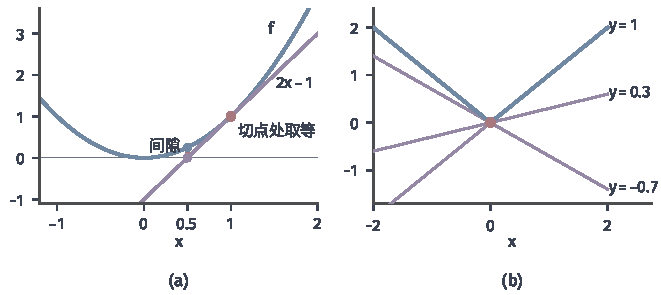
\includegraphics[width=112mm]{figures/05-optimization/06-constrained-optimization/matplotlib/dual-fenchel-young/figure.pdf}
 \caption{Fenchel--Young不等式的几何。(a)~蓝线是$f(x)=x^2$，紫线是$y=2$的最高下界$2x-1$，红色短线是$x=0.5$处的间隙$0.25$，红点$x=1$处间隙为零。(b)~蓝线是$\lvert x\rvert$，紫线是$y=-0.7,0.3,1$的下界，它们都在红点$x=0$处贴着折线，所以这些$y$都是$0$处的次梯度。}
 \label{fig:dual-fenchel-young}
\end{BookInlineFigure}

共轭把$f$变成了一族下方的直线。这些直线够不够重建$f$？把共轭再做一次，得到\term{双共轭}（biconjugate）
\begin{equation}
 f^{**}(\bm{x})=\sup_{\bm{y}}\bigl\{\langle\bm{y},\bm{x}\rangle-f^*(\bm{y})\bigr\},
 \label{eq:dual-biconjugate}
\end{equation}
它是$f$全部仿射下界的上确界。由式~\eqref{eq:dual-fenchel-young}，总有$f^{**}\leq f$。反过来的不等式需要在$f$上方的每个缺口处放进一条直线，工具是分离定理。

\begin{theorem}[点与闭凸集的严格分离]
 \label{thm:dual-separation}
 设$\bm{S}\subseteq\mathbb{R}^N$非空、闭、凸，$\bm{z}\notin\bm{S}$。则存在$\bm{a}\neq\bm{0}$和$\beta\in\mathbb{R}$，使得对所有$\bm{w}\in\bm{S}$，
 \begin{equation}
  \langle\bm{a},\bm{w}\rangle\leq\beta<\langle\bm{a},\bm{z}\rangle.
  \label{eq:dual-separation}
 \end{equation}
\end{theorem}

\begin{proof}
 第~\ref{chap:nonsmooth-composite-optimization}章已得到投影$\bm{p}=\Pi_{\bm{S}}(\bm{z})$的存在性及其刻画：
 \[
  \langle\bm{z}-\bm{p},\bm{w}-\bm{p}\rangle\leq0\qquad\text{对所有}\ \bm{w}\in\bm{S}.
 \]
 令$\bm{a}=\bm{z}-\bm{p}$，$\beta=\langle\bm{a},\bm{p}\rangle$。$\bm{z}\notin\bm{S}$而$\bm{p}\in\bm{S}$，所以$\bm{a}\neq\bm{0}$。上式就是$\langle\bm{a},\bm{w}\rangle\leq\beta$。又因为
 \[
  \langle\bm{a},\bm{z}\rangle=\beta+\lVert\bm{a}\rVert_2^2>\beta,
 \]
 式~\eqref{eq:dual-separation}成立。
\end{proof}

超平面$\{\bm{w}:\langle\bm{a},\bm{w}\rangle=\beta\}$称为\term{分离超平面}（separating hyperplane）。把分离定理用到函数上，要把函数变成集合。函数$f$的\term{上图}（epigraph）是
\[
 \operatorname{epi}f=\{(\bm{x},r):\bm{x}\in\operatorname{dom}f,\ r\geq f(\bm{x})\}.
\]
$f$凸时上图凸。$f$下半连续时上图闭：若$(\bm{x}^{(k)},r^{(k)})\to(\bm{x},r)$且$r^{(k)}\geq f(\bm{x}^{(k)})$，则$r\geq\liminf_kf(\bm{x}^{(k)})\geq f(\bm{x})$。

\begin{theorem}[Fenchel--Moreau]
 \label{thm:dual-fenchel-moreau}
 设$f:\mathbb{R}^n\to\mathbb{R}\cup\{+\infty\}$是适当、下半连续的凸函数，则$f^{**}=f$。
\end{theorem}

\begin{proof}
 已知$f^{**}\leq f$，只需证明：对任意$\bm{x}$和任意实数$r<f(\bm{x})$，存在仿射下界$\ell\leq f$使$\ell(\bm{x})>r$。因为若$\ell(\cdot)=\langle\bm{y},\cdot\rangle-\beta'$是这样的下界，由$\ell\leq f$得$f^*(\bm{y})\leq\beta'$，于是$f^{**}(\bm{x})\geq\ell(\bm{x})>r$。

 点$(\bm{x},r)$不在闭凸集$\operatorname{epi}f$中。对它应用定理~\ref{thm:dual-separation}，并把分离向量取相反数，得到$(\bm{a},b)\neq\bm{0}$和$\beta$，使对所有$(\bm{x}',r')\in\operatorname{epi}f$，
 \[
  \langle\bm{a},\bm{x}'\rangle+br'\geq\beta>\langle\bm{a},\bm{x}\rangle+br.
 \]
 上图沿$r'$向上无界，所以$b\geq0$。

 情形一：$b>0$。取$r'=f(\bm{x}')$并除以$b$，得到仿射下界
 \[
  \ell(\bm{x}')=\frac{\beta-\langle\bm{a},\bm{x}'\rangle}{b}\leq f(\bm{x}'),
 \]
 而分离的严格不等式正是$\ell(\bm{x})>r$。若$\bm{x}\in\operatorname{dom}f$，一定属于这一情形，否则$b=0$时取$\bm{x}'=\bm{x}$，$r'=f(\bm{x})$，得到矛盾：
 \[
  \langle\bm{a},\bm{x}\rangle\geq\beta>\langle\bm{a},\bm{x}\rangle.
 \]

 情形二：$b=0$，此时$\bm{x}\notin\operatorname{dom}f$，并且对所有$\bm{x}'\in\operatorname{dom}f$有$\beta-\langle\bm{a},\bm{x}'\rangle\leq0$。在$\operatorname{dom}f$中任取一点用情形一，得到某个仿射下界$\ell_0\leq f$。对$\varepsilon>0$令
 \[
  \ell_\varepsilon(\bm{x}')=\ell_0(\bm{x}')+\frac{\beta-\langle\bm{a},\bm{x}'\rangle}{\varepsilon}.
 \]
 在$\operatorname{dom}f$上第二项非正，所以$\ell_\varepsilon\leq f$。在点$\bm{x}$处$\beta-\langle\bm{a},\bm{x}\rangle>0$，$\varepsilon$足够小时$\ell_\varepsilon(\bm{x})>r$。
\end{proof}

定理的三个条件各有作用。图~\ref{fig:dual-biconjugate}(a)和(b)说明闭性的作用。$f=\iota_{(0,1)}$是凸函数，但不是下半连续的，因为端点处函数值跳到$+\infty$。它的共轭和双共轭分别是
\[
 f^*(y)=\sup_{0<x<1}xy=\max\{y,0\},\qquad f^{**}=\iota_{[0,1]}.
\]
双共轭补上了两个端点，因为仿射下界分辨不出开区间和它的闭包。

凸性的作用见图~\ref{fig:dual-biconjugate}(c)。双井函数$(x^2-1)^2$的双共轭在$[-1,1]$上是$0$，中间的鼓包被抹平了。一般地，只要$f$有仿射下界，$f^{**}$就是$f$的最大的下半连续凸下界，仿射下界只能看到函数的凸的部分。

\begin{BookInlineFigure}
 \centering
 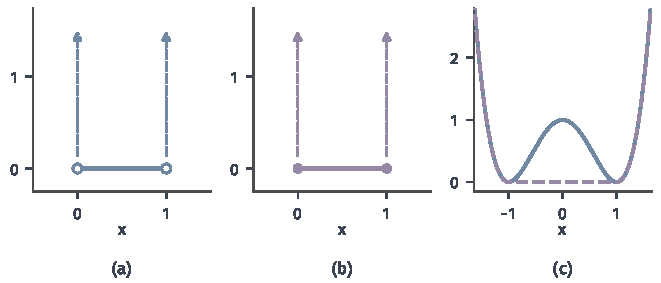
\includegraphics[width=112mm]{figures/05-optimization/06-constrained-optimization/matplotlib/dual-biconjugate/figure.pdf}
 \caption{双共轭恢复什么。(a)~$\iota_{(0,1)}$，两端的空心点表示不属于有效定义域，虚线箭头表示区间外为$+\infty$。(b)~它的双共轭$\iota_{[0,1]}$，端点变为实心。(c)~蓝线是双井函数$(x^2-1)^2$，紫色虚线是数值计算的双共轭，在$[-1,1]$上为零，在外侧与原函数重合。}
 \label{fig:dual-biconjugate}
\end{BookInlineFigure}

定理~\ref{thm:dual-fenchel-moreau}说的是一个函数可以由它的仿射下界重建，并没有说某个约束问题的对偶间隙为零。后者涉及目标和约束的联合结构，要到下一节才能回答，两件事不能混淆。

\subsection{对偶形式的推导}
\label{sec:dual-forms}

有了共轭，对偶函数可以按公式写出，不必每次重新配方。先看线性等式约束$\bm{A}\bm{x}=\bm{b}$，其中$\bm{A}\in\mathbb{R}^{p\times n}$。把内层的线性项按定义~\eqref{eq:dual-conjugate}改写：
\[
 \inf_{\bm{x}}\bigl\{f(\bm{x})+\langle\bm{A}^\top\bm{\nu},\bm{x}\rangle\bigr\}=-\sup_{\bm{x}}\bigl\{\langle-\bm{A}^\top\bm{\nu},\bm{x}\rangle-f(\bm{x})\bigr\}.
\]
右端的上确界是$f^*(-\bm{A}^\top\bm{\nu})$，于是
\begin{equation}
 q(\bm{\nu})=-f^*(-\bm{A}^\top\bm{\nu})-\bm{b}^\top\bm{\nu}.
 \label{eq:dual-q-conj}
\end{equation}

符号要逐项记住：共轭的自变量带负号，因为$\inf$变$\sup$时线性项反号。式~\eqref{eq:dual-q-conj}有限的条件是$-\bm{A}^\top\bm{\nu}\in\operatorname{dom}f^*$，也就是说，共轭的有限范围就是对偶问题的隐含约束。

用二次例核对。$\bm{Q}=\operatorname{diag}(1,4)$，$\bm{A}=(1,1)$，$b=1$。由式~\eqref{eq:dual-conj-quadratic}，
\[
 f^*(-\nu,-\nu)=\frac12\Bigl(\nu^2+\frac{\nu^2}{4}\Bigr)=\frac58\nu^2.
\]
代入式~\eqref{eq:dual-q-conj}得到$q(\nu)=-\frac58\nu^2-\nu$，与式~\eqref{eq:dual-quad-q}相同。

\paragraph{复合形式}
第~\ref{chap:nonsmooth-composite-optimization}章常见的目标是两部分之和，一部分作用在$\bm{x}$上，另一部分作用在$\bm{A}\bm{x}$上：
\begin{equation}
 \min_{\bm{x}}\ F(\bm{x})=f(\bm{x})+g(\bm{A}\bm{x}),
 \label{eq:dual-composite}
\end{equation}
其中$g:\mathbb{R}^p\to\mathbb{R}\cup\{+\infty\}$是一个函数，不是约束函数$g_i$，$\bm{A}\in\mathbb{R}^{p\times n}$。这个问题没有显式的约束，直接写Lagrange函数得不到任何东西。

办法是人为造出一条约束：引入辅助变量$\bm{z}=\bm{A}\bm{x}$，把问题改写成
\[
 \min_{\bm{x},\bm{z}}\ f(\bm{x})+g(\bm{z})\quad\text{s.t.}\quad\bm{A}\bm{x}-\bm{z}=\bm{0}.
\]
这是等价改写，最优值不变。给等式配乘子$\bm{\nu}\in\mathbb{R}^p$，Lagrange函数按$\bm{x}$和$\bm{z}$分成两部分：
\[
 \mathcal{L}=\bigl[f(\bm{x})+\langle\bm{A}^\top\bm{\nu},\bm{x}\rangle\bigr]+\bigl[g(\bm{z})-\langle\bm{\nu},\bm{z}\rangle\bigr].
\]

两部分的下确界可以分别取。第一部分和前面相同，第二部分由共轭的定义得到：
\[
 \inf_{\bm{x}}\bigl[f(\bm{x})+\langle\bm{A}^\top\bm{\nu},\bm{x}\rangle\bigr]=-f^*(-\bm{A}^\top\bm{\nu}),\qquad
 \inf_{\bm{z}}\bigl[g(\bm{z})-\langle\bm{\nu},\bm{z}\rangle\bigr]=-g^*(\bm{\nu}).
\]
于是得到\term{Fenchel对偶}（Fenchel duality）：
\begin{equation}
 \max_{\bm{\nu}}\ q(\bm{\nu})=-f^*(-\bm{A}^\top\bm{\nu})-g^*(\bm{\nu}).
 \label{eq:dual-fenchel}
\end{equation}

图~\ref{fig:dual-composite-flow}是这个推导的结构。注意$\bm{\nu}$在两项里符号相反，这是从$\bm{A}\bm{x}-\bm{z}$的两个系数来的：换成$\bm{z}-\bm{A}\bm{x}$，等于把$\bm{\nu}$换成$-\bm{\nu}$，最优值不变。

\begin{BookInlineFigure}
 \centering
 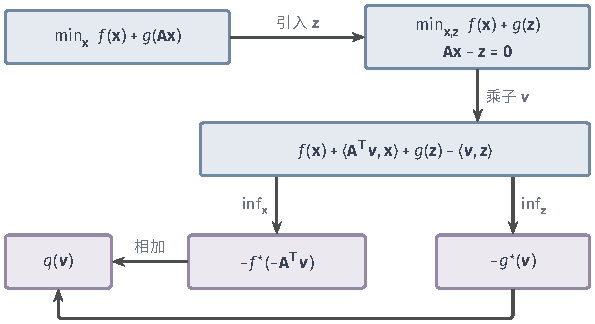
\includegraphics[width=100.8mm]{figures/05-optimization/06-constrained-optimization/tikz/dual-composite-flow/figure.pdf}
 \caption{复合问题的对偶形式怎样得到。浅蓝框是原变量一侧的表达，浅紫框是对偶一侧的量：引入$\bm{z}$，配乘子$\bm{\nu}$，再对$\bm{x}$和$\bm{z}$分别取下确界，得到两个共轭。}
 \label{fig:dual-composite-flow}
\end{BookInlineFigure}

式~\eqref{eq:dual-fenchel}的弱对偶也可以直接从Fenchel--Young不等式看出。对任意$\bm{x}$和$\bm{\nu}$，把式~\eqref{eq:dual-fenchel-young}分别用于$(f,\bm{x},-\bm{A}^\top\bm{\nu})$和$(g,\bm{A}\bm{x},\bm{\nu})$，得到
\[
 f(\bm{x})+f^*(-\bm{A}^\top\bm{\nu})\geq-\langle\bm{A}\bm{x},\bm{\nu}\rangle,\qquad
 g(\bm{A}\bm{x})+g^*(\bm{\nu})\geq\langle\bm{A}\bm{x},\bm{\nu}\rangle.
\]
两式相加，右端抵消，即得$F(\bm{x})\geq q(\bm{\nu})$。

下面算一个例子，目标沿用预算例的二次项，第二项换成绝对值惩罚：
\[
 \min_{\bm{x}\in\mathbb{R}^2}\ \frac12\bigl[(x_1-2)^2+(x_2-1)^2\bigr]+\lvert x_1+x_2\rvert.
\]
这里$\bm{A}=(1,1)$，$g=\lvert\cdot\rvert$，$\bm{a}=(2,1)$，$f(\bm{x})=\frac12\lVert\bm{x}-\bm{a}\rVert_2^2$。

先求$f^*$。上确界的驻点是$\bm{x}=\bm{a}+\bm{y}$，代入得到
\[
 f^*(\bm{y})=\langle\bm{y},\bm{a}\rangle+\frac12\lVert\bm{y}\rVert_2^2.
\]
取$\bm{y}=-\bm{A}^\top\nu=(-\nu,-\nu)$，有
\[
 f^*(-\bm{A}^\top\nu)=-3\nu+\nu^2.
\]

由表~\ref{tab:dual-conjugates}，$g^*=\iota_{[-1,1]}$，它的作用是把$\nu$限制在$[-1,1]$内。于是对偶问题是
\[
 \max_{-1\leq\nu\leq1}\ 3\nu-\nu^2.
\]
无约束最大点$\nu=3/2$在区间外，所以$\nu^\star=1$，对偶值是$3-1=2$。

回到原变量。由$\bm{x}$的驻定条件$\bm{x}-\bm{a}+\bm{A}^\top\nu=\bm{0}$，得到
\[
 \bm{x}=\bm{a}-\bm{A}^\top\nu^\star=(1,0).
\]
核对目标值：$F(1,0)=\frac12(1+1)+1=2$，等于对偶值。根据弱对偶，$(1,0)$是最优解。这里零间隙是算出来的；一般情况下式~\eqref{eq:dual-fenchel}只建立了对偶的表达，零间隙能否成立，要看下一节的条件。

\section{强对偶}
\label{sec:dual-strong}

前面的二次例、预算例和绝对值例中，最好的下界都恰好等于最优值。于是要问：这在什么时候成立？当$d^\star=f^\star$时，称\term{强对偶}成立，也说零间隙。这里有三件容易混淆的事要分开：两个最优值相等，原始最优点存在，最优乘子存在。

\paragraph{联合集合与分离}
为了看清楚乘子从哪里来，把目标和约束放到同一个空间里。定义联合集合
\begin{equation}
 \bm{A}=\bigl\{(\bm{u},\bm{w},t):\text{存在}\ \bm{x}\in\bm{D}\ \text{使}\ g_i(\bm{x})\leq u_i,\ h_j(\bm{x})=w_j,\ f(\bm{x})\leq t\bigr\}.
 \label{eq:dual-joint-set}
\end{equation}
$(\bm{u},\bm{w})$是约束右端允许的松动量，$t$是能够达到的目标值。原问题的最优值是集合$\bm{A}$在$(\bm{u},\bm{w})=\bm{0}$这条竖线上的最低高度。

$\bm{\lambda}\geq\bm{0}$时，对偶函数可以用这个集合重写：
\[
 q(\bm{\lambda},\bm{\nu})=\inf_{(\bm{u},\bm{w},t)\in\bm{A}}\bigl\{t+\langle\bm{\lambda},\bm{u}\rangle+\langle\bm{\nu},\bm{w}\rangle\bigr\}.
\]
所以$q$是用法向量$(\bm{\lambda},\bm{\nu},1)$的超平面从下方托住$\bm{A}$时，在竖轴上的高度。$f,g_i$凸且$h_j$仿射时$\bm{A}$是凸集，分离定理就有了用武之地。

设想把一张纸从下方贴到$\bm{A}$上，碰在点$(\bm{0},f^\star)$处。如果纸不是竖直的，就可以把法向量的$t$分量归一成$1$，其余分量就是乘子，竖轴上的高度就是$f^\star$，强对偶成立。所以问题的关键是这张纸是否竖直。

图~\ref{fig:dual-joint-set}对比两种情形，只有一条不等式，$\bm{A}$位于平面上。(a)是一元例，$\bm{A}$的下边界是最优值函数$v(u)=\frac12\max\{1-u,0\}^2$。它在$u=0$的两侧都有定义，切线$t=\frac12-u$的斜率给出$\lambda^\star=1$。

(b)是问题$\min x$，约束$x^2\leq u$。$u<0$时不可行，$v(u)=-\sqrt{u}$在$u=0$处切线竖直。能托住$\bm{A}$并经过原点的只有竖直线，它不对应任何有限的乘子。

\begin{BookInlineFigure}
 \centering
 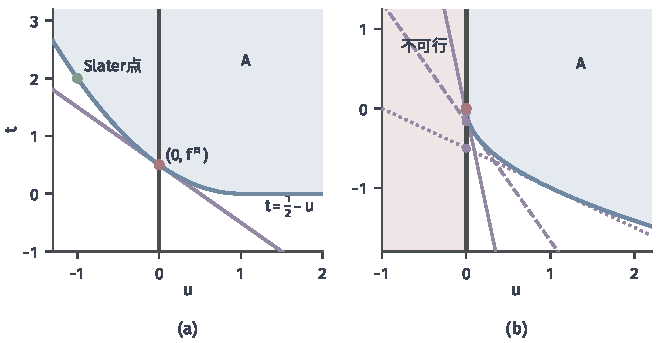
\includegraphics[width=112mm]{figures/05-optimization/06-constrained-optimization/matplotlib/dual-joint-set/figure.pdf}
 \caption{联合集合$\bm{A}$（浅蓝）与托住它的直线。(a)~一元例：紫线$t=\frac12-u$在红点$(0,f^\star)$处托住$\bm{A}$，斜率对应$\lambda^\star=1$；绿点是Slater点$x=0$对应的$(g,f)=(-1,2)$，它在竖线$u=0$的左侧。(b)~$\min x$，约束$x^2\leq u$：浅红区域$u<0$不可行，$\bm{A}$的边界在红点处切线竖直，紫线是$\lambda=0.5,1.5,5$（点线、虚线、实线）的托线，交点高度$-1/(4\lambda)$随$\lambda$增大升向$0$，但能经过红点的只有深灰色竖线。}
 \label{fig:dual-joint-set}
\end{BookInlineFigure}

要排除竖直的纸，只需要$\bm{A}$在竖线左侧确实有点，这正是图~\ref{fig:dual-joint-set}(a)中绿点起的作用。

\subsection{Slater条件}
\label{sec:dual-slater}

把上面的想法写成条件。设$f,g_i:\mathbb{R}^n\to\mathbb{R}\cup\{+\infty\}$是凸函数，等式约束仿射，写成$\bm{A}\bm{x}=\bm{b}$，其中$\bm{A}\in\mathbb{R}^{p\times n}$。共同有效定义域是
\[
 \bm{D}=\operatorname{dom}f\cap\bigcap_i\operatorname{dom}g_i.
\]
第~\ref{chap:nonsmooth-composite-optimization}章用$\operatorname{ri}$表示相对内部，即在集合自身的仿射包内的内点。

\begin{definition}[Slater条件]
 \label{def:dual-slater}
 若存在$\bar{\bm{x}}\in\operatorname{ri}\bm{D}$，使
 \begin{equation}
  g_i(\bar{\bm{x}})<0,\quad i=1,\ldots,m,\qquad\bm{A}\bar{\bm{x}}=\bm{b},
  \label{eq:dual-slater}
 \end{equation}
 就称问题满足\term{Slater条件}（Slater's condition），$\bar{\bm{x}}$称为Slater点。
\end{definition}

条件的每一部分都有用处。严格不等式让点落在竖线左侧；等式约束无法严格，只要求满足；取在相对内部，是为了让定义域在$\bar{\bm{x}}$周围留有余地，否则余量可能恰好被定义域的边缘吃掉。

三个例子都容易找到Slater点。一元例取$\bar{x}=0$，$g(\bar{x})=-1<0$。预算例取$\bar{\bm{x}}=(1/2,1/2)$，它在$\bm{D}=\mathbb{R}^2_{+}$的内部，且$x_1+x_2-2=-1<0$。二次例没有不等式，取约束直线上的任一点。

证明要分离的不是闭集，$(\bm{0},f^\star)$可能就在$\bm{A}$的边界上。定理~\ref{thm:dual-separation}不够用，需要下面这个不要求闭性、也不要求严格的版本。

\begin{lemma}[点与凸集的分离]
 \label{lem:dual-separation-convex}
 设$\bm{S}\subseteq\mathbb{R}^N$非空、凸，$\bm{z}\notin\bm{S}$。则存在$\bm{a}\neq\bm{0}$，使得对所有$\bm{w}\in\bm{S}$，
 \begin{equation}
  \langle\bm{a},\bm{w}\rangle\geq\langle\bm{a},\bm{z}\rangle.
  \label{eq:dual-separation-convex}
 \end{equation}
\end{lemma}

\begin{proof}
 $\mathbb{R}^N$的子集有可数稠密子集，取$\bm{S}$中的这样一列点$\bm{w}_1,\bm{w}_2,\ldots$。对每个$k$，令$\bm{S}_k$是$\bm{w}_1,\ldots,\bm{w}_k$的凸组合全体。

 $\bm{S}_k$是单纯形在连续映射下的像，所以是紧的，从而是闭集；它包含于凸集$\bm{S}$，所以不含$\bm{z}$。对$\bm{S}_k$用定理~\ref{thm:dual-separation}，取相反数并归一化，得到单位向量$\bm{a}_k$，使
 \[
  \langle\bm{a}_k,\bm{w}_j\rangle>\langle\bm{a}_k,\bm{z}\rangle,\qquad j=1,\ldots,k.
 \]

 单位球面是紧集，$\bm{a}_k$有收敛子列，极限$\bm{a}$仍是单位向量。固定$j$，让$k$沿子列趋于无穷，得到
 \[
  \langle\bm{a},\bm{w}_j\rangle\geq\langle\bm{a},\bm{z}\rangle.
 \]
 $\{\bm{w}_j\}$在$\bm{S}$中稠密，内积连续，所以式~\eqref{eq:dual-separation-convex}对全部$\bm{w}\in\bm{S}$成立。
\end{proof}

\begin{theorem}[Slater条件下的强对偶]
 \label{thm:dual-slater}
 设问题的$f,g_i$凸、等式约束仿射，满足Slater条件，且$f^\star$有限。则
 \begin{equation}
  d^\star=f^\star,
  \label{eq:dual-strong}
 \end{equation}
 并且对偶最优值被某组$(\bm{\lambda}^\star,\bm{\nu}^\star)$达到，其中$\bm{\lambda}^\star\geq\bm{0}$。
\end{theorem}

\begin{proof}
 第一步，选取工作空间。令$\bm{V}$是$\bm{D}$的仿射包的方向子空间，$\bm{W}=\{\bm{A}\bm{v}:\bm{v}\in\bm{V}\}$。对$\bm{x}\in\bm{D}$，由$\bm{A}\bar{\bm{x}}=\bm{b}$，有
 \[
  \bm{A}\bm{x}-\bm{b}=\bm{A}(\bm{x}-\bar{\bm{x}})\in\bm{W}.
 \]
 所以等式残差不会离开$\bm{W}$，只需要在$\mathbb{R}^m\times\bm{W}\times\mathbb{R}$中讨论。

 第二步，构造被分离的集合。令$\bm{S}$是满足下面条件的$(\bm{u},\bm{w},t)$的全体：存在$\bm{x}\in\bm{D}$，使$g_i(\bm{x})\leq u_i$，$\bm{A}\bm{x}-\bm{b}=\bm{w}$，$f(\bm{x})<t$。由$f,g_i$的凸性和等式的仿射性，$\bm{S}$是凸集，并且它是非空的，因为$\bar{\bm{x}}\in\bm{D}$。点$(\bm{0},\bm{0},f^\star)$不在$\bm{S}$中，否则存在可行点使$f(\bm{x})<f^\star$。

 第三步，应用分离。由引理~\ref{lem:dual-separation-convex}，存在不全为零的$\bm{\lambda}\in\mathbb{R}^m$、$\bm{\nu}\in\bm{W}$、$\lambda_0\in\mathbb{R}$，使对所有$(\bm{u},\bm{w},t)\in\bm{S}$，
 \[
  \langle\bm{\lambda},\bm{u}\rangle+\langle\bm{\nu},\bm{w}\rangle+\lambda_0t\geq\lambda_0f^\star.
 \]
 $\bm{S}$中的点可以把$u_i$或$t$任意增大，若$\lambda_i<0$或$\lambda_0<0$，左端会趋于$-\infty$，所以$\bm{\lambda}\geq\bm{0}$，$\lambda_0\geq0$。

 任取$\bm{x}\in\bm{D}$，取$\bm{u}=(g_i(\bm{x}))_i$，$\bm{w}=\bm{A}\bm{x}-\bm{b}$，$t=f(\bm{x})+\varepsilon$，令$\varepsilon\downarrow0$，得到
 \[
  \sum_i\lambda_ig_i(\bm{x})+\langle\bm{\nu},\bm{A}\bm{x}-\bm{b}\rangle+\lambda_0f(\bm{x})\geq\lambda_0f^\star,\qquad\bm{x}\in\bm{D}.
 \]

 第四步，证明$\lambda_0>0$，也就是这张纸不竖直。设$\lambda_0=0$。把$\bm{x}=\bar{\bm{x}}$代入上式，等式项为零，得到
 \[
  \sum_i\lambda_ig_i(\bar{\bm{x}})\geq0.
 \]
 由$g_i(\bar{\bm{x}})<0$和$\bm{\lambda}\geq\bm{0}$，只能$\bm{\lambda}=\bm{0}$。于是$\bm{\nu}\neq\bm{0}$，并且上式变成对所有$\bm{x}\in\bm{D}$，
 \[
  \langle\bm{\nu},\bm{A}(\bm{x}-\bar{\bm{x}})\rangle\geq0.
 \]
 因为$\bar{\bm{x}}\in\operatorname{ri}\bm{D}$，存在$r>0$，使对$\bm{v}\in\bm{V}$，$\lVert\bm{v}\rVert_2\leq r$，都有$\bar{\bm{x}}+\bm{v}\in\bm{D}$。代入$\pm\bm{v}$，得到$\langle\bm{\nu},\bm{A}\bm{v}\rangle=0$，也就是$\bm{\nu}$与$\bm{W}$正交。而$\bm{\nu}\in\bm{W}$，所以$\bm{\nu}=\bm{0}$，矛盾。

 第五步，构造乘子。令$\bm{\lambda}^\star=\bm{\lambda}/\lambda_0$，$\bm{\nu}^\star=\bm{\nu}/\lambda_0$，除以$\lambda_0$，上面第三步的不等式成为对所有$\bm{x}\in\bm{D}$，
 \[
  \mathcal{L}(\bm{x},\bm{\lambda}^\star,\bm{\nu}^\star)\geq f^\star.
 \]
 对$\bm{x}$取下确界，
 \[
  q(\bm{\lambda}^\star,\bm{\nu}^\star)\geq f^\star.
 \]
 由弱对偶，
 \[
  q(\bm{\lambda}^\star,\bm{\nu}^\star)\leq d^\star\leq f^\star.
 \]
 所以三者相等，并且这组乘子达到$d^\star$。
\end{proof}

证明里Slater点只在第四步用到，这正是前面“排除竖直的纸”的严格写法。定理的结论并不包括原始最优点存在，这一点在第~\ref{sec:dual-gap-attainment}节用例子说明。Slater点本身可行，所以$f^\star<+\infty$，有限的假设只是排除$f^\star=-\infty$；这时弱对偶迫使$d^\star=-\infty$，对偶可行的乘子不存在，也就谈不上最优乘子。

如果某些$g_i$本身是仿射的，这些约束不必严格满足，只要$g_i(\bar{\bm{x}})\leq0$，其余要求不变。原因在于仿射约束的集合是多面体，分离时不会出现图~\ref{fig:dual-joint-set}(b)那样切线竖直的边缘，这与线性规划不需要严格可行点的道理相同。证明需要用到多面体凸集的分离，篇幅较长，读者可查阅\scite{rockafellar1970convex}。全部约束都仿射、目标线性时，这就是第~\ref{chap:linear-programming}章已经证明的强对偶。

\subsection{共轭对偶的正则条件}
\label{sec:dual-regularity}

复合问题~\eqref{eq:dual-composite}没有不等式，不等式上的“严格可行”没有对应物，正则条件要换一种说法。回忆它的改写形式：变量$(\bm{x},\bm{z})$，有效定义域是$\operatorname{dom}f\times\operatorname{dom}g$，约束是线性等式。Slater条件要求的是存在满足等式、位于定义域相对内部的点。乘积集的仿射包是各因子仿射包的乘积，所以乘积集的相对内部等于各因子相对内部的乘积，这就翻译成了下面的条件。

\begin{theorem}[Fenchel对偶的强对偶]
 \label{thm:dual-fenchel-strong}
 设$f:\mathbb{R}^n\to\mathbb{R}\cup\{+\infty\}$，$g:\mathbb{R}^p\to\mathbb{R}\cup\{+\infty\}$是适当、下半连续的凸函数，$\bm{A}\in\mathbb{R}^{p\times n}$。若存在$\bm{x}$使
 \begin{equation}
  \bm{x}\in\operatorname{ri}(\operatorname{dom}f),\qquad\bm{A}\bm{x}\in\operatorname{ri}(\operatorname{dom}g),
  \label{eq:dual-fenchel-regular}
 \end{equation}
 且式~\eqref{eq:dual-composite}的最优值$F^\star$有限，则$\sup_{\bm{\nu}}q(\bm{\nu})=F^\star$，其中$q$由式~\eqref{eq:dual-fenchel}给出，并且对偶最优值被达到。
\end{theorem}

\begin{proof}
 把定理~\ref{thm:dual-slater}用于改写形式，变量是$(\bm{x},\bm{z})$，目标是$f(\bm{x})+g(\bm{z})$，等式是$\bm{A}\bm{x}-\bm{z}=\bm{0}$，没有不等式。若$\bm{x}$满足式~\eqref{eq:dual-fenchel-regular}，则$(\bm{x},\bm{A}\bm{x})$在定义域的相对内部且满足等式，是Slater点。改写形式的对偶函数正是式~\eqref{eq:dual-fenchel}。
\end{proof}

证明中没有用到下半连续。这个假设保证$f^{**}=f$和$g^{**}=g$，使$q$对应的对偶问题再取一次对偶时能回到原问题，所以通常写在一起。定理保证的是两个最优值相等、对偶最优乘子存在，原始问题的最小点是否存在，要另外用强制性或紧性论证。

上一节的绝对值例中$\operatorname{dom}f=\mathbb{R}^2$，$\operatorname{dom}g=\mathbb{R}$，两个定义域都是全空间，条件自动满足，所以那里的零间隙在算出结果之前就可以预知。

条件中的相对内部不是形式要求，看一个定义域只在边界上相遇的例子。取$f(x)=-\sqrt{x}$（$x\geq0$，其余为$+\infty$），$g=\iota_{\{0\}}$，$A=1$。此时要求$x\in(0,\infty)$且$x=0$，式~\eqref{eq:dual-fenchel-regular}不成立。可行点只有$x=0$，所以$F^\star=0$。

对偶一侧，$g^*=0$。$\nu>0$时$f^*(-\nu)=\sup_{x\geq0}\{-\nu x+\sqrt{x}\}$在$\sqrt{x}=1/(2\nu)$处达到，于是
\[
 f^*(-\nu)=\frac{1}{4\nu},\qquad q(\nu)=-\frac{1}{4\nu}.
\]
$\nu\leq0$时$f^*(-\nu)=+\infty$。所以$\sup q=0=F^\star$，零间隙仍然成立，但上确界取不到，对偶最优乘子不存在。

\subsection{间隙与达到的区别}
\label{sec:dual-gap-attainment}

“强对偶成立”“原始最优点存在”“最优乘子存在”是三件不同的事。本小节用三个例子分别让其中一件出问题，表~\ref{tab:dual-gap-cases}是它们的汇总。

第一个例子最小化$e^{-x}$，约束$-x\leq0$。Slater点$x=1$存在，$f^\star=0$有限，定理~\ref{thm:dual-slater}适用。第~\ref{sec:dual-function}节已经算出$q(0)=0$，其余$q(\lambda)=-\infty$，于是
\[
 d^\star=0=f^\star,\qquad\lambda^\star=0.
\]
零间隙成立，乘子达到，但没有$x$能使$e^{-x}=0$，原始最优值不达到。图~\ref{fig:dual-three-failures}(a)是这个函数，它只在无穷远处靠近下确界。

第二个例子最小化$x$，约束$x^2\leq0$。唯一的可行点是$x=0$，所以$f^\star=0$，原始最优点存在。Slater条件不成立，因为$x^2<0$无解。

对$\lambda>0$，$x+\lambda x^2$在$x=-1/(2\lambda)$处最小，$\lambda=0$时下确界为$-\infty$。于是
\[
 q(\lambda)=-\frac{1}{4\lambda}\quad(\lambda>0).
\]
$\lambda\to+\infty$时$q\to0$，所以$d^\star=0=f^\star$，零间隙成立，但没有有限的$\lambda$能达到。如图~\ref{fig:dual-three-failures}(b)，这正是图~\ref{fig:dual-joint-set}(b)中切线竖直的代价。

这个例子还说明，第~\ref{chap:constrained-optimality}章在同一问题上看到的“最小点没有KKT乘子”，与“对偶最优值取不到”是同一件事的两面。

第三个例子的定义域是$\bm{D}=\{\bm{x}\in\mathbb{R}^2:x_2>0\}$，问题是
\[
 \min_{\bm{x}\in\bm{D}}\ e^{-x_1}\quad\text{s.t.}\quad\frac{x_1^2}{x_2}\leq0.
\]
函数$x_1^2/x_2$在$x_2>0$上是凸的，这可以由Hessian半正定验证，所以这是一个凸问题。约束迫使$x_1=0$，于是$f^\star=1$，并在$\{0\}\times(0,\infty)$上达到。

求对偶函数。对任意$\lambda\geq0$，内层函数$e^{-x_1}+\lambda x_1^2/x_2$总是正的，所以$q(\lambda)\geq0$。沿曲线$x_1=s$，$x_2=s^3$，令$s\to+\infty$，有
\[
 e^{-s}+\frac{\lambda}{s}\to0.
\]
所以$q(\lambda)=0$对所有$\lambda\geq0$成立，$d^\star=0$。

两个最优值分别是$1$和$0$，对偶间隙为$1$。这说明凸性本身不能保证零间隙。Slater条件在这里失败，因为$x_1^2/x_2<0$无解。

图~\ref{fig:dual-three-failures}(c)显示了联合集合的样子：最优值函数$v$在$u=0$处的值是$1$，而$u>0$时只要让$x_1,x_2$都增大，就有$x_1^2/x_2\leq u$，目标值可以任意接近$0$，所以$v(u)=0$。$v$在$u=0$处有一个跳跃，从下方托住$\bm{A}$的直线最高只能到$0$。

\begin{BookInlineFigure}
 \centering
 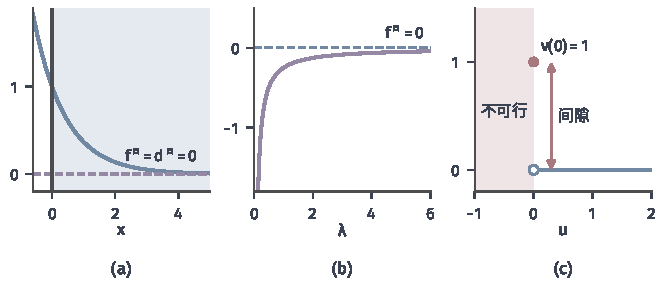
\includegraphics[width=112mm]{figures/05-optimization/06-constrained-optimization/matplotlib/dual-three-failures/figure.pdf}
 \caption{三种不同的情形。(a)~蓝线是$e^{-x}$，浅蓝区域可行，下确界$0$不被取到，紫色虚线是$d^\star$。(b)~$\min x$，约束$x^2\leq0$的对偶函数$q(\lambda)=-1/(4\lambda)$，向蓝色虚线$f^\star=0$靠近但取不到。(c)~第三个例子的最优值函数：浅红区域$u<0$不可行，红点是$v(0)=1$，$u>0$时$v(u)=0$，空心点表示$u=0$时下极限，红色箭头是对偶间隙$1$。}
 \label{fig:dual-three-failures}
\end{BookInlineFigure}

\begin{BookInlineTable}
 \centering
 \begin{tabular}{@{}llllll@{}}
  \toprule
  问题 & Slater & $f^\star$ & $d^\star$ & 原始达到 & 对偶达到\\
  \midrule
  $\min e^{-x}$，$-x\leq0$ & 成立 & $0$ & $0$ & 否 & 是\\
  $\min x$，$x^2\leq0$ & 不成立 & $0$ & $0$ & 是 & 否\\
  $\min e^{-x_1}$，$x_1^2/x_2\leq0$ & 不成立 & $1$ & $0$ & 是 & 是\\
  \bottomrule
 \end{tabular}
 \caption{间隙与达到的三个例子。第三个例子全部乘子都是对偶最优的。}
 \label{tab:dual-gap-cases}
\end{BookInlineTable}

表中第二行和第三行都不满足Slater条件，结局却不同：一个零间隙，一个正间隙。所以Slater条件只是充分条件，不成立时要具体分析。

\section{最优性证书}
\label{sec:dual-certificates}

前面分别得到了下界、KKT条件和强对偶。接下来要弄清：手上有一对原始—对偶候选，怎样判断它已经解决了原问题，这几种工具各自检验了什么？

先看一个不能只信对偶一侧的例子。设$\bm{D}=[0,1]$，
\[
 \min_{x\in[0,1]}\ -x\quad\text{s.t.}\quad x-\frac12\leq0.
\]
目标要求$x$尽量大，约束限制$x$不超过$1/2$，所以解是$x^\star=1/2$，$f^\star=-1/2$。Lagrange函数对$x$是线性的，下确界在$\bm{D}$的端点取得，比较$x=0$和$x=1$两处的值，得到
\[
 q(\lambda)=\min\Bigl\{-\frac{\lambda}{2},\ \frac{\lambda}{2}-1\Bigr\}.
\]

$\lambda^\star=1$是这条折线的最高点，$q(1)=-1/2=f^\star$，强对偶成立。一个只盯着对偶目标的算法到这里就停止了。但它手里的原变量是内层的最小点：$\lambda<1$时是$x=1$，$\lambda>1$时是$x=0$，如图~\ref{fig:dual-recover-fail}(b)所示。

$x=1$不可行，$x=0$可行但目标值是$0$，比$f^\star$差。$\lambda=1$时内层的最小点是整个$[0,1]$，$x^\star$只是其中一点，内层本身挑不出它。所以乘子停止改进不等于原问题解完了，求出的候选必须回到原问题上检验。

\begin{BookInlineFigure}
 \centering
 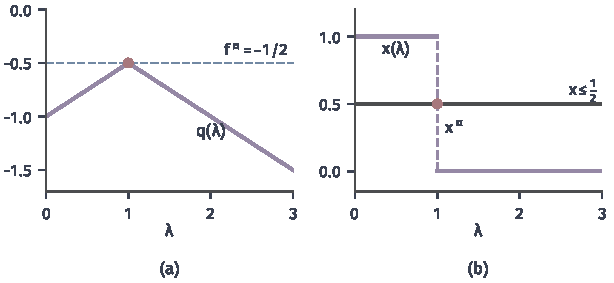
\includegraphics[width=104mm]{figures/05-optimization/06-constrained-optimization/matplotlib/dual-recover-fail/figure.pdf}
 \caption{对偶最优不等于得到了原始解。(a)~紫线是折线$q(\lambda)$，红点是对偶最优点$\lambda^\star=1$，蓝色虚线是$f^\star$。(b)~紫线是内层最小点$x(\lambda)$，它在$\lambda=1$处从$1$跳到$0$，紫色虚线表示此时最小点是整个区间；深灰粗线是约束边界，红点是$x^\star$，内层解不会自动落到它上面。}
 \label{fig:dual-recover-fail}
\end{BookInlineFigure}

\subsection{零间隙与KKT}
\label{sec:dual-zero-gap-kkt}

可以检验的证据是一对候选加上零间隙。第~\ref{chap:constrained-optimality}章的KKT条件是在候选点$\bm{x}$处的四组关系：$\bm{x}$可行；$\bm{\lambda}\geq\bm{0}$；互补松弛$\lambda_ig_i(\bm{x})=0$；以及Lagrange函数对$\bm{x}$驻定，
\[
 \nabla f(\bm{x})+\sum_i\lambda_i\nabla g_i(\bm{x})+\sum_j\nu_j\nabla h_j(\bm{x})=\bm{0}.
\]
那里证明了，凸问题的KKT点是全局最小点。下面把这个结论与零间隙联系起来。

\begin{theorem}[零间隙与KKT]
 \label{thm:dual-zero-gap-kkt}
 考虑问题~\eqref{eq:dual-primal}。

 第一，设$\bm{x}^\star$可行，$\bm{\lambda}^\star\geq\bm{0}$，且
 \begin{equation}
  f(\bm{x}^\star)=q(\bm{\lambda}^\star,\bm{\nu}^\star).
  \label{eq:dual-zero-gap}
 \end{equation}
 则$\bm{x}^\star$原始全局最优，$(\bm{\lambda}^\star,\bm{\nu}^\star)$对偶最优，互补松弛成立，并且$\bm{x}^\star$在$\bm{D}$上全局最小化$\mathcal{L}(\cdot,\bm{\lambda}^\star,\bm{\nu}^\star)$。若各函数在$\bm{x}^\star$处可微且$\bm{x}^\star\in\operatorname{int}\bm{D}$，则$(\bm{x}^\star,\bm{\lambda}^\star,\bm{\nu}^\star)$满足KKT条件。

 第二，设$\bm{D}$是开凸集，$f,g_i$在其上凸且可微，$h_j$仿射，$(\bm{x}^\star,\bm{\lambda}^\star,\bm{\nu}^\star)$满足KKT条件。则式~\eqref{eq:dual-zero-gap}成立，原始、对偶两侧都最优。
\end{theorem}

\begin{proof}
 第一部分。由弱对偶，
 \[
  f(\bm{x}^\star)=q(\bm{\lambda}^\star,\bm{\nu}^\star)\leq d^\star\leq f^\star\leq f(\bm{x}^\star),
 \]
 各处取等，所以两侧都最优。

 再写一条链，由$q$的定义和可行性，
 \[
  q(\bm{\lambda}^\star,\bm{\nu}^\star)\leq\mathcal{L}(\bm{x}^\star,\bm{\lambda}^\star,\bm{\nu}^\star)=f(\bm{x}^\star)+\sum_i\lambda_i^\star g_i(\bm{x}^\star)\leq f(\bm{x}^\star).
 \]
 两端相等，所以两个不等号都取等。第二个不等号取等给出
 \[
  \sum_i\lambda_i^\star g_i(\bm{x}^\star)=0.
 \]
 每一项非正，因此每一项都是零，这就是互补松弛。

 第一个不等号取等，说明$\mathcal{L}(\bm{x}^\star,\bm{\lambda}^\star,\bm{\nu}^\star)$等于它在$\bm{D}$上的下确界，即$\bm{x}^\star$是全局最小点。若$\bm{x}^\star$是$\bm{D}$的内点且函数可微，梯度为零就是驻定条件。

 第二部分。$\lambda_i^\star\geq0$且$h_j$仿射，所以$\mathcal{L}(\cdot,\bm{\lambda}^\star,\bm{\nu}^\star)$在$\bm{D}$上是凸函数，驻点就是全局最小点。于是由互补松弛和可行性，
 \[
  q(\bm{\lambda}^\star,\bm{\nu}^\star)=\mathcal{L}(\bm{x}^\star,\bm{\lambda}^\star,\bm{\nu}^\star)=f(\bm{x}^\star).
 \]
 再用第一部分即得结论。
\end{proof}

定理的第一部分不要求凸性，这是最通用的最优性证据，并且把KKT作为一个推论给出来。用预算例核对：$\bm{x}^\star=(3/2,1/2)$可行，$\lambda^\star=1/2$，由式~\eqref{eq:dual-budget-q}有$q(1/2)=1/4=f(\bm{x}^\star)$，所以这一对候选的最优性得到了证明，不需要知道解是怎样算出来的。

反过来就要小心了。非凸问题的Lagrange驻定不代表内层全局最小，定理第二部分的凸性假设不能省略。看$\min-x^2$，约束$x-1\leq0$和$-x-1\leq0$。图~\ref{fig:dual-nonconvex-kkt}(a)标出了三个KKT点：$x=0$（乘子全为零）和$x=\pm1$。

$x=0$的目标值是$0$，它甚至是一个局部最大点，KKT只把它列为候选。$x=1$是真正的全局最小点，由驻定条件$-2+\lambda_1=0$得$\lambda_1=2$，$\lambda_2=0$。此时
\[
 \mathcal{L}(x,2,0)=-x^2+2(x-1)=-(x-1)^2-1.
\]
这条开口向下的抛物线在$x=1$处是\emph{最大}点，如图~\ref{fig:dual-nonconvex-kkt}(b)。$q(2,0)=-\infty$，这一对KKT候选的候选间隙是$+\infty$。

所以即便$x=1$确实最优，这组乘子也给不出证书。换一种约束写法，结果又不同。把可行集写成$x^2-1\leq0$，则
\[
 \mathcal{L}(x,\lambda)=(\lambda-1)x^2-\lambda,\qquad q(\lambda)=-\lambda\quad(\lambda\geq1).
\]
$\lambda=1$时$q=-1=f^\star$，零间隙成立。可行集完全相同，对偶却依赖约束的写法，这也是非凸问题的一个特点。

\begin{BookInlineFigure}
 \centering
 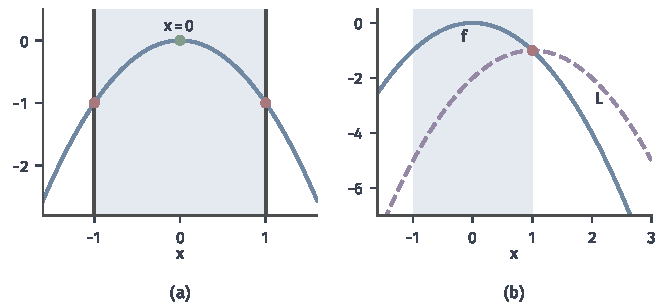
\includegraphics[width=112mm]{figures/05-optimization/06-constrained-optimization/matplotlib/dual-nonconvex-kkt/figure.pdf}
 \caption{非凸问题的KKT点不等于零间隙候选。(a)~$\min-x^2$，浅蓝区域是$[-1,1]$，红点是全局最优点$x=\pm1$，绿点是KKT点$x=0$，它是局部最大点。(b)~蓝线是$f$，紫色虚线是$\mathcal{L}(\cdot,2,0)=-(x-1)^2-1$，它在红点$x=1$处驻定，但那里是最大点，$\mathcal{L}$没有下界。}
 \label{fig:dual-nonconvex-kkt}
\end{BookInlineFigure}

\subsection{Lagrange鞍点}
\label{sec:dual-saddle}

上面的证书也可以用一个不等式组写出，它把原始和对偶两个问题放在对称的位置上。关键的一步，是发现原问题本身也能用$\mathcal{L}$写出来。固定$\bm{x}\in\bm{D}$，对乘子取上确界：
\begin{equation}
 \sup_{\bm{\lambda}\geq\bm{0},\ \bm{\nu}}\mathcal{L}(\bm{x},\bm{\lambda},\bm{\nu})=\begin{cases}f(\bm{x}), & \bm{x}\ \text{可行},\\+\infty, & \bm{x}\ \text{不可行}.\end{cases}
 \label{eq:dual-sup-recovers}
\end{equation}

理由是：若某条$g_i(\bm{x})>0$，令$\lambda_i\to+\infty$；若某条$h_j(\bm{x})\neq0$，令$\nu_j\to\pm\infty$，都趋于$+\infty$。若$\bm{x}$可行，$\lambda_ig_i\leq0$且$\nu_jh_j=0$，取$\bm{\lambda}=\bm{0}$就达到上确界$f(\bm{x})$。这就是开头说的“硬墙”：把价格抬到无穷大，就重新得到了硬约束。

所以原问题是$\inf_{\bm{x}}\sup_{\bm{\lambda},\bm{\nu}}\mathcal{L}$，对偶问题是$\sup_{\bm{\lambda},\bm{\nu}}\inf_{\bm{x}}\mathcal{L}$，两者只差取极值的次序，弱对偶正是一般的不等式$\sup\inf\leq\inf\sup$。图~\ref{fig:dual-saddle}(b)用一元例画出了式~\eqref{eq:dual-sup-recovers}：$x=0$可行，直线随$\lambda$下降，上确界在$\lambda=0$处取到$f(0)=2$；$x=1.5$不可行，直线向上趋于无穷。

\begin{definition}[Lagrange鞍点]
 \label{def:dual-saddle}
 设$\bm{x}^\star\in\bm{D}$，$\bm{\lambda}^\star\geq\bm{0}$。若对所有$\bm{x}\in\bm{D}$、$\bm{\lambda}\geq\bm{0}$、$\bm{\nu}$都有
 \begin{equation}
  \mathcal{L}(\bm{x}^\star,\bm{\lambda},\bm{\nu})\leq\mathcal{L}(\bm{x}^\star,\bm{\lambda}^\star,\bm{\nu}^\star)\leq\mathcal{L}(\bm{x},\bm{\lambda}^\star,\bm{\nu}^\star),
  \label{eq:dual-saddle}
 \end{equation}
 就称$(\bm{x}^\star,\bm{\lambda}^\star,\bm{\nu}^\star)$是\term{Lagrange鞍点}（Lagrangian saddle point）。
\end{definition}

式~\eqref{eq:dual-saddle}的右半边是全局最小，不是局部驻定，这是它与KKT的关键区别。图~\ref{fig:dual-saddle}(a)是一元例中$\mathcal{L}(x,\lambda)$的等高线，$(1,1)$是鞍点。沿绿色虚线（固定$\lambda=1$）$\mathcal{L}$在$x=1$处最小，见图~\ref{fig:dual-saddle}(c)；沿紫色虚线（固定$x=1$）$\mathcal{L}$恒为$\frac12$，这时左半边取等。

\begin{BookInlineFigure}
 \centering
 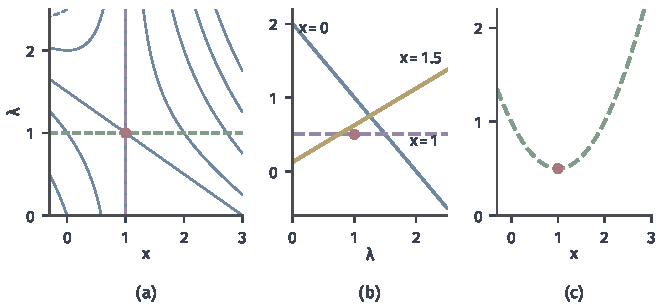
\includegraphics[width=112mm]{figures/05-optimization/06-constrained-optimization/matplotlib/dual-saddle/figure.pdf}
 \caption{一元例的Lagrange鞍点。(a)~蓝线是$\mathcal{L}(x,\lambda)=\frac12(x-2)^2+\lambda(x-1)$的等高线，红点是鞍点$(1,1)$，绿色虚线固定$\lambda=1$，紫色虚线固定$x=1$。(b)~固定$x$时$\mathcal{L}$关于$\lambda$的直线：蓝线$x=0$可行，黄线$x=1.5$不可行，紫色虚线是$x=1$。(c)~固定$\lambda=1$时关于$x$的抛物线，红点是最小点。}
 \label{fig:dual-saddle}
\end{BookInlineFigure}

\begin{theorem}[鞍点等价于两侧达到且零间隙]
 \label{thm:dual-saddle}
 $(\bm{x}^\star,\bm{\lambda}^\star,\bm{\nu}^\star)$是Lagrange鞍点，当且仅当$\bm{x}^\star$是原始最优点，$(\bm{\lambda}^\star,\bm{\nu}^\star)$是对偶最优乘子，并且式~\eqref{eq:dual-zero-gap}成立。此结论不要求问题凸。
\end{theorem}

\begin{proof}
 必要性。记鞍点处的Lagrange函数值为$\mathcal{L}^\star$。式~\eqref{eq:dual-saddle}左半边说明$\mathcal{L}(\bm{x}^\star,\cdot,\cdot)$对乘子有上界，由式~\eqref{eq:dual-sup-recovers}，$\bm{x}^\star$可行，并且上确界$f(\bm{x}^\star)\leq\mathcal{L}^\star$。

 由$\bm{\lambda}^\star\geq\bm{0}$和可行性，又有$\mathcal{L}^\star\leq f(\bm{x}^\star)$，所以
 \[
  \mathcal{L}^\star=f(\bm{x}^\star).
 \]
 式~\eqref{eq:dual-saddle}右半边说明$\bm{x}^\star$是$\mathcal{L}(\cdot,\bm{\lambda}^\star,\bm{\nu}^\star)$在$\bm{D}$上的全局最小点，所以
 \[
  q(\bm{\lambda}^\star,\bm{\nu}^\star)=\mathcal{L}^\star=f(\bm{x}^\star).
 \]
 由定理~\ref{thm:dual-zero-gap-kkt}第一部分，两侧都最优。

 充分性。设$\bm{x}^\star$可行，$\bm{\lambda}^\star\geq\bm{0}$，且式~\eqref{eq:dual-zero-gap}成立。由定理~\ref{thm:dual-zero-gap-kkt}第一部分，互补松弛成立，所以$\mathcal{L}^\star=f(\bm{x}^\star)$，且$\bm{x}^\star$全局最小化$\mathcal{L}(\cdot,\bm{\lambda}^\star,\bm{\nu}^\star)$，这是右半边。对任意$\bm{\lambda}\geq\bm{0}$和$\bm{\nu}$，由可行性，
 \[
  \mathcal{L}(\bm{x}^\star,\bm{\lambda},\bm{\nu})=f(\bm{x}^\star)+\sum_i\lambda_ig_i(\bm{x}^\star)\leq f(\bm{x}^\star)=\mathcal{L}^\star,
 \]
 这是左半边。
\end{proof}

由定理~\ref{thm:dual-saddle}，鞍点存在需要两个最优值都达到并且相等，这比强对偶强。第~\ref{sec:dual-gap-attainment}节前两个例子零间隙，却都没有鞍点，因为其中一侧没有达到。

把驻定当成鞍点是常见的错误。上一小节的$(1,2,0)$使$\nabla_x\mathcal{L}=0$，但$x=1$是$\mathcal{L}$的最大点，这组点满足KKT，却不满足式~\eqref{eq:dual-saddle}的右半边。一般的极小极大问题中交换取极值次序的条件，由第~\ref{chap:minimax-optimization}章专门研究，这里的$\mathcal{L}$对乘子是线性的，是其中结构较简单的一类。

图~\ref{fig:dual-certificate-map}和表~\ref{tab:dual-certificate-compare}把这一节的关系放在一起。中间的结论只有一个：一对候选，两边都全局最优，且目标值相等。

\begin{BookInlineFigure}
 \centering
 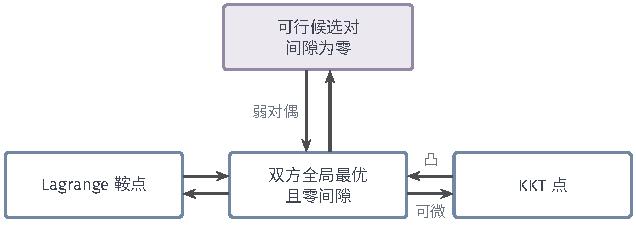
\includegraphics[width=107.8mm]{figures/05-optimization/06-constrained-optimization/tikz/dual-certificate-map/figure.pdf}
 \caption{几种最优性证据的关系。零间隙的可行候选对与“双方全局最优且零间隙”等价，后者与Lagrange鞍点等价，这三者都不要求凸性；从KKT点推出中间结论需要凸性，从中间结论推出KKT点需要在内点处可微。}
 \label{fig:dual-certificate-map}
\end{BookInlineFigure}

\begin{BookInlineTable}
 \centering
 \begin{tabular}{@{}lll@{}}
  \toprule
  证据 & 要检查什么 & 能断言什么\\
  \midrule
  KKT & 可行、符号、互补、驻定 & 凸时才全局最优\\
  候选间隙 & 可行、合法乘子、可信的$q$ & 次优性不超过间隙\\
  零间隙 & 同上，且间隙为零 & 两侧全局最优\\
  鞍点 & 式~\eqref{eq:dual-saddle}，右半为全局最小 & 与零间隙候选对等价\\
  \bottomrule
 \end{tabular}
 \caption{几种最优性证据的比较。除KKT外，其余三种证据都不要求问题凸。}
 \label{tab:dual-certificate-compare}
\end{BookInlineTable}

\section{本章小结}
\label{sec:dual-summary}

本章开头的问题是，手里有一个可行点，怎样知道它离最优还差多少。回答是对偶函数：固定一组合法乘子，对原变量在整个定义域上取下确界，得到的数就是最优值的下界。这个下界只用了下确界的定义和符号，所以弱对偶不需要凸性、可微性和约束资格。对偶函数总是凹的，但计算它的每个值都要做一次内层全局最小化。

一对候选给出的误差证书$f(\hat{\bm{x}})-q(\bm{\lambda},\bm{\nu})$有三个前提：原始可行，乘子合法，$q$算得可信。内层近似得到的值在真正的下界上方，必须扣除经过证明的误差，才能写进证书。

凸共轭把“函数加线性项取下确界”单独提取出来，二次函数、范数、约束指标函数的共轭分别对应二次项、对偶范数球和支撑函数，由此可以直接写出线性约束问题和复合问题的对偶形式。共轭能够重建适当、下半连续的凸函数，但这一点与某个具体问题的零间隙是两回事。

最好的下界是否等于最优值，取决于正则条件。Slater条件和复合问题的相对内部条件都排除了竖直的支撑超平面，保证零间隙和对偶最优乘子存在，却不保证原始最优点存在。凸性本身不能保证零间隙，零间隙也不保证两侧都达到。

实际使用时，能够核对的证据是一对候选加上间隙。零间隙的候选对同时给出两侧的全局最优性，等价于Lagrange鞍点，这些结论不要求凸性；KKT点在凸问题中才等价于它们。乘子如何解释参数的变化，由第~\ref{chap:parametric-sensitivity}章讨论；怎样在算法中实际更新乘子，由第~\ref{chap:penalty-multiplier-methods}章讨论。


\chapter{参数敏感性}
\label{chap:parametric-sensitivity}

一笔预算要分给两种投入。预算从$2$增加到$2.1$，最优的损失能下降多少？理想配置改变一点，最优配置又往哪里移动？这些问题里，变的不是求解过程，而是问题本身。

把新问题重新解一遍当然可以得到答案，但它只回答一个具体的数。我们还想知道：多一单位预算值多少钱，这个价钱在多大范围内可信，几个参数同时变化时不重新求解能否估计结果，以及什么时候这样的估计根本不成立。

本章区分两个输出。最优值是一个数，它的变化可以由对偶乘子给出对任意大小扰动都成立的下界，也可以由包络关系给出局部导数。最优解是一个向量，它的移动要把最优性条件看成方程，用隐函数定理求导，因而需要更强的条件。

第~\ref{sec:sens-problems}节先说清参数变化时比较的是什么对象。第~\ref{sec:sens-value}节研究最优值，第~\ref{sec:sens-solution}节研究最优解，全章用同一个预算二次问题来核对公式。局部导数并不总是存在，第~\ref{sec:sens-branches}节用可以手算的例子拆开三种失效的原因。第~\ref{sec:sens-computation}节讨论怎样计算这些导数，又怎样检验算出的导数可信。

\section{含参问题}
\label{sec:sens-problems}

参数变化之后，“解的变化”到底指什么？本节要先回答这个问题。参数一变，问题可能没有解，也可能有许多解，所以必须先把比较的对象定义清楚。

\paragraph{贯穿全章的预算二次例}
沿用第~\ref{chap:constrained-optimality}章的预算分配。两种投入的数量是$x_1$、$x_2$，它们非负，总量不超过预算$\tau$。理想配置是$(2,1)$，偏离理想配置按平方计算损失。于是得到问题
\begin{equation}
 \min_{\bm{x}\in\mathbb{R}^2}\ \frac12(x_1-2)^2+\frac12(x_2-1)^2
 \quad\text{s.t.}\quad x_1+x_2\leq\tau,\ \ x_1\geq0,\ \ x_2\geq0.
 \label{eq:sens-budget}
\end{equation}
为了和一般记号对应，把三条约束写成$g_1=x_1+x_2-\tau$、$g_2=-x_1$、$g_3=-x_2$，都要求不大于零，相应的乘子是$\lambda_1,\lambda_2,\lambda_3$。

这个问题有清楚的几何图景。目标的等高线是以理想点$\bm{c}=(2,1)$为圆心的同心圆，所以最优解就是可行三角形里离$\bm{c}$最近的点。预算线像一堵可以平移的墙，$\tau$增大时墙向外退，三角形变大。

图~\ref{fig:sens-budget-family}画出三个预算水平。$\tau=4$时墙退得很远，碗底$(2,1)$本身可行，没有约束起作用。$\tau=2$时碗底被挡在墙外，解落在预算线上的$(3/2,1/2)$。$\tau=0.5$时三角形很小，解被挤到角点$(0.5,0)$，预算和$x_2\geq0$同时起作用。

\begin{BookInlineFigure}
 \centering
 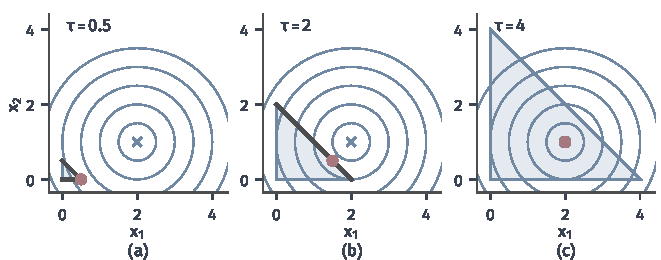
\includegraphics[width=112mm]{figures/05-optimization/06-constrained-optimization/matplotlib/sens-budget-family/figure.pdf}
 \caption{预算二次例~\eqref{eq:sens-budget}在三个预算下的情形。浅蓝三角形是可行集，蓝色同心圆是目标等高线，蓝色叉是理想点$(2,1)$，红点是最优解，深灰粗线是起作用的约束。(a)~$\tau=0.5$，预算和$x_2\geq0$都起作用。(b)~$\tau=2$，只有预算起作用。(c)~$\tau=4$，没有约束起作用。}
 \label{fig:sens-budget-family}
\end{BookInlineFigure}

\paragraph{变量与参数}
式~\eqref{eq:sens-budget}里有两类量。$\bm{x}$由优化决定，$\tau$由外部给定，求解时保持不变。前者是我们的选择，后者是我们所处的环境。同一个量算变量还是参数，取决于建模时想回答什么：若预算也可以选择，它就应该成为变量。

把环境写成参数向量$\bm{\theta}$，每个$\bm{\theta}$确定一个优化问题，全体构成一族问题。研究这族问题，需要两个输出对象。

\begin{definition}[含参问题、最优值函数与解映射]
\label{def:sens-family}
设$\bm{\Theta}\subseteq\mathbb{R}^q$是参数集合。对每个$\bm{\theta}\in\bm{\Theta}$，给定可行集$\bm{C}(\bm{\theta})\subseteq\mathbb{R}^n$和目标$f(\cdot,\bm{\theta})$，称
\begin{equation}
 \min_{\bm{x}\in\bm{C}(\bm{\theta})}f(\bm{x},\bm{\theta})
 \label{eq:sens-family}
\end{equation}
为\term{含参问题}（parametric problem）。函数
\begin{equation}
 V(\bm{\theta})=\inf_{\bm{x}\in\bm{C}(\bm{\theta})}f(\bm{x},\bm{\theta})
 \label{eq:sens-value}
\end{equation}
称为\term{最优值函数}（value function），并约定空集上的下确界为$+\infty$。把每个参数对应到最优解集合的映射
\begin{equation}
 \bm{S}(\bm{\theta})=\bigl\{\bm{x}\in\bm{C}(\bm{\theta}):f(\bm{x},\bm{\theta})=V(\bm{\theta})\bigr\}
 \label{eq:sens-solution-map}
\end{equation}
称为\term{解映射}（solution map）。
\end{definition}

$V$和$\bm{S}$的性格很不一样。$V(\bm{\theta})$总是一个确定的量，只是可能取$\pm\infty$。$\bm{S}(\bm{\theta})$是一个集合，可能是空集，可能只有一个点，也可能有无穷多个点。对预算例，$\tau<0$时可行集是空集，所以$V(\tau)=+\infty$，$\bm{S}(\tau)=\varnothing$。$\tau\geq0$时目标强凸、可行集紧，$\bm{S}(\tau)$恰有一个点。

\paragraph{参数改变可能使问题失去解}
除了不可行，参数改变还可能让最小值取不到。下面的一族问题定义在整条实轴上：
\[
 \min_{x\in\mathbb{R}}\ f(x,\theta)=e^{x}-\theta x.
\]
图~\ref{fig:sens-three-outcomes}画出三种情况，下面逐个计算。

\begin{BookInlineFigure}
 \centering
 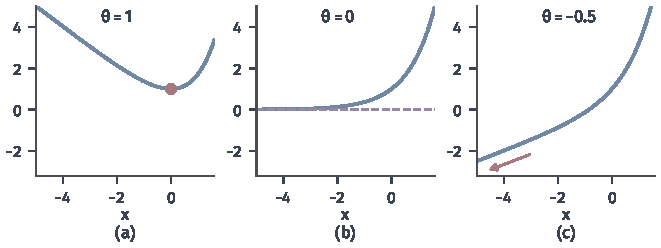
\includegraphics[width=112mm]{figures/05-optimization/06-constrained-optimization/matplotlib/sens-three-outcomes/figure.pdf}
 \caption{同一族目标$f(x,\theta)=e^{x}-\theta x$在三个参数下的结果。(a)~$\theta=1$，最小值$1$在红点$x=0$取得。(b)~$\theta=0$，下确界$0$（紫色虚线）有限但取不到。(c)~$\theta=-0.5$，红色箭头表示目标沿$x\to-\infty$无下界。}
 \label{fig:sens-three-outcomes}
\end{BookInlineFigure}

$\theta>0$时，令导数$e^x-\theta$为零，得到唯一的驻点$x=\ln\theta$。二阶导数$e^x$为正，所以它是全局极小点，并且
\[
 V(\theta)=\theta-\theta\ln\theta,\qquad \bm{S}(\theta)=\{\ln\theta\}.
\]

$\theta=0$时目标是$e^x$，它的下确界是$0$，但没有点取得这个值，所以$V(0)=0$而$\bm{S}(0)=\varnothing$。$\theta<0$时，$x\to-\infty$使$-\theta x=\lvert\theta\rvert x\to-\infty$，而$e^x\to0$，所以$V(\theta)=-\infty$。

这族问题还显示出值与解的差别。$\theta\downarrow0$时，$V(\theta)=\theta-\theta\ln\theta\to0=V(0)$，值的变化是连续的。解却是$\ln\theta\to-\infty$，一路跑向无穷远。讨论变化之前，必须先确认所研究的$\bm{\theta}$处解存在，并说明比较的是值还是解。

\paragraph{有多个解时要说清跟踪谁}
考虑一个有两个山谷的目标：
\begin{equation}
 f(x,\theta)=(x^2-1)^2+\theta x.
 \label{eq:sens-double-well}
\end{equation}
$\theta=0$时两个谷底$x=\pm1$同样低，$\bm{S}(0)=\{-1,1\}$。$\theta$不为零时，$\theta x$这一项把地面倾斜，一个谷底升高，另一个降低。“最优解对$\theta$的导数”这句话在$\theta=0$处没有明确含义，因为不知道说的是哪一个解。

这时有两种办法把问题说清楚。一种是跟踪一条\term{局部极小分支}（local minimizer branch），即在$\bm{\theta}_0$的邻域上定义的映射$\bm{x}(\bm{\theta})$，使每个$\bm{x}(\bm{\theta})$都是相应问题的局部极小点，并且随$\bm{\theta}$连续变化。另一种是约定\term{选解规则}（selection rule），例如总取最优解中范数最小的一个。

沿分支的目标值记作
\begin{equation}
 v(\bm{\theta})=f(\bm{x}(\bm{\theta}),\bm{\theta}).
 \label{eq:sens-branch-value}
\end{equation}
小写的$v$是某条分支上的值，大写的$V$是全局最优值。分支上的点都可行，所以$v(\bm{\theta})\geq V(\bm{\theta})$，只有分支恰好全局最优时才取等号。

图~\ref{fig:sens-double-well}展示了这种区别。(b)中两条绿色虚线是两个谷底的位置，它们各自光滑。红色实线是全局最优解，它在$\theta=0$处从上面一条跳到下面一条。(c)中分支的值光滑地穿过$\theta=0$，全局最优值是两者中较小的那个，在$\theta=0$处有折角。例如沿右侧谷底的分支在$\theta>0$时仍然是局部极小，但它的值已经高于全局最优值，不能称为“最优值”。

\begin{BookInlineFigure}
 \centering
 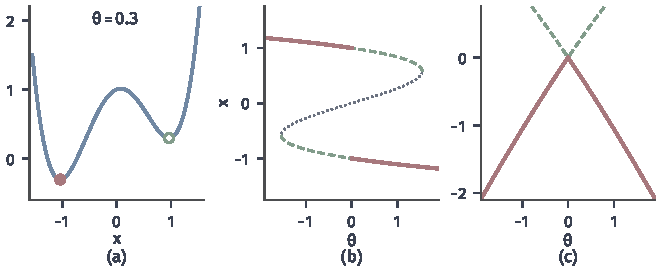
\includegraphics[width=112mm]{figures/05-optimization/06-constrained-optimization/matplotlib/sens-double-well/figure.pdf}
 \caption{双谷目标~\eqref{eq:sens-double-well}的分支与全局解。(a)~$\theta=0.3$时的目标，红点是全局最小点，绿色空心点是另一个局部极小点。(b)~驻点随$\theta$的变化：绿色虚线是局部极小分支，灰色点线是局部极大分支，红色实线是全局最优解。(c)~绿色虚线是两条分支上的目标值，红色实线是全局最优值。}
 \label{fig:sens-double-well}
\end{BookInlineFigure}

图~\ref{fig:sens-objects}汇总这些对象的关系。本章每个结论都会说明针对哪一个对象：是全局的$V$，还是某条分支上的$v$；是整个解集合$\bm{S}$，还是分支$\bm{x}(\bm{\theta})$。

\begin{BookInlineFigure}
 \centering
 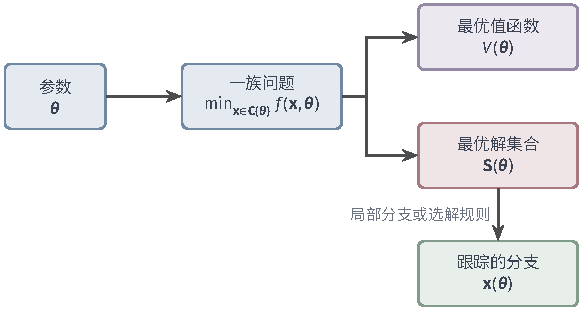
\includegraphics[width=99mm]{figures/05-optimization/06-constrained-optimization/tikz/sens-objects/figure.pdf}
 \caption{含参问题的三个输出对象。参数确定一个优化问题，问题确定最优值函数和最优解集合。解集合可能为空或含多个点，只有通过局部分支或选解规则，才得到一个随参数变化的点。}
 \label{fig:sens-objects}
\end{BookInlineFigure}

\section{最优值的变化}
\label{sec:sens-value}

参数变了以后，最优值变化多少？本节研究这个问题。先让约束的右端变化，乘子会给出一个对任意大小的扰动都成立的下界；再让目标和约束显含一般的参数，这时得到的是局部导数。“下界的斜率”“实际的导数”“方向导数”是三个不同的量，下面逐个说明它们各自成立的条件。

\subsection{约束右端的全局变化界}
\label{sec:sens-rhs-bound}

\paragraph{扰动右端}
对一般约束问题，在每条约束的右端加上扰动，定义
\begin{equation}
 V(\bm{u},\bm{v})=\inf\bigl\{f(\bm{x}):\ g_i(\bm{x})\leq u_i,\ h_j(\bm{x})=v_j,\ \forall i,j\bigr\}.
 \label{eq:sens-rhs-value}
\end{equation}
这里$\bm{u}\in\mathbb{R}^m$，$\bm{v}\in\mathbb{R}^p$，不可行时$V=+\infty$。基准问题的最优值是$f^\star=V(\bm{0},\bm{0})$。$u_i>0$把第$i$条不等式放宽，$u_i<0$把它收紧。

\paragraph{按旧价格结算}
第~\ref{chap:duality}章的Lagrange函数是
\[
 \mathcal{L}(\bm{x},\bm{\lambda},\bm{\nu})=f(\bm{x})+\sum_{i=1}^m\lambda_ig_i(\bm{x})+\sum_{j=1}^p\nu_jh_j(\bm{x}),
\]
对偶函数是
\[
 q(\bm{\lambda},\bm{\nu})=\inf_{\bm{x}}\mathcal{L}(\bm{x},\bm{\lambda},\bm{\nu}).
\]
弱对偶说$\bm{\lambda}\geq\bm{0}$时$q(\bm{\lambda},\bm{\nu})\leq f^\star$，强对偶且乘子达到则说存在$(\bm{\lambda}^\star,\bm{\nu}^\star)$，使$q(\bm{\lambda}^\star,\bm{\nu}^\star)=f^\star$。

可以把乘子想成一张事先定好的价格表：用$g_i(\bm{x})$这么多资源，就按$\lambda_i^\star$的单价结算。强对偶达到的意思是，在这张价格表下，每一个点$\bm{x}$的结算额$\mathcal{L}(\bm{x},\bm{\lambda}^\star,\bm{\nu}^\star)$都不低于$f^\star$。若右端变了，新问题的可行点仍然要按这张旧价格表结算，结算额的下限不变，由此就得到新最优值的下界。

\begin{theorem}[最优值的全局下界]
\label{thm:sens-rhs-bound}
设基准问题的最优值$f^\star$有限，存在$\bm{\lambda}^\star\geq\bm{0}$与$\bm{\nu}^\star$，使$q(\bm{\lambda}^\star,\bm{\nu}^\star)=f^\star$。则对所有$(\bm{u},\bm{v})\in\mathbb{R}^m\times\mathbb{R}^p$，
\begin{equation}
 V(\bm{u},\bm{v})\geq f^\star-\langle\bm{\lambda}^\star,\bm{u}\rangle-\langle\bm{\nu}^\star,\bm{v}\rangle.
 \label{eq:sens-rhs-bound}
\end{equation}
\end{theorem}

\begin{proof}
若扰动问题不可行，左端是$+\infty$，结论成立。否则任取扰动问题的可行点$\bm{x}$。由$q$的定义，
\[
 f^\star=q(\bm{\lambda}^\star,\bm{\nu}^\star)\leq\mathcal{L}(\bm{x},\bm{\lambda}^\star,\bm{\nu}^\star).
\]

把Lagrange函数展开。由$\lambda_i^\star\geq0$和$g_i(\bm{x})\leq u_i$，第$i$个不等式项不超过$\lambda_i^\star u_i$。由$h_j(\bm{x})=v_j$，等式项正好等于$\nu_j^\star v_j$。于是
\[
 f^\star\leq f(\bm{x})+\langle\bm{\lambda}^\star,\bm{u}\rangle+\langle\bm{\nu}^\star,\bm{v}\rangle.
\]
移项后对所有可行的$\bm{x}$取下确界，就得到式~\eqref{eq:sens-rhs-bound}。
\end{proof}

式~\eqref{eq:sens-rhs-bound}的右端是$(\bm{u},\bm{v})$的仿射函数，它在原点与$V$相等，在其他地方不超过$V$。第$i$条不等式方向上，下界的斜率是$-\lambda_i^\star$，负号来自“右端增大意味着约束放宽”。放宽$u_i>0$时，最优值至多下降$\lambda_i^\star u_i$。收紧$u_i<0$时，最优值至少上升$\lambda_i^\star\lvert u_i\rvert$。

\paragraph{条件各起什么作用}
定理没有要求问题是凸的，也没有要求函数可微，证明里只用了不等式。它也不要求扰动后的解和基准解有相同的活动约束，甚至不要求解存在。所以这是一个全局结论，对很大的扰动同样成立，只是方向是单侧的。

定理还有一个推论：在这些条件下，任何右端扰动都不会使问题变得无下界，因为式~\eqref{eq:sens-rhs-bound}的右端总是有限的。

\paragraph{预算例的验证}
取基准预算$\tau=2$，令$u=\tau-2$，只扰动第一条约束。基准解是$\bm{x}^\star=(3/2,1/2)$，后两条约束不起作用。乘子取$\bm{\lambda}^\star=(1/2,0,0)$，此时Lagrange函数是
\[
 \mathcal{L}(\bm{x},\bm{\lambda}^\star)=\frac12(x_1-2)^2+\frac12(x_2-1)^2+\frac12(x_1+x_2-2).
\]

这是关于$\bm{x}$的强凸二次函数。令梯度为零，得到$x_1-2+\tfrac12=0$与$x_2-1+\tfrac12=0$，极小点恰好是$(3/2,1/2)$。把它代入，因为$x_1+x_2-2=0$，所以
\[
 q(\bm{\lambda}^\star)=\frac12\cdot\frac14+\frac12\cdot\frac14=\frac14=f^\star.
\]

零间隙得到验证，强对偶和乘子达到都成立。式~\eqref{eq:sens-rhs-bound}于是给出：对所有$\tau$，
\begin{equation}
 V(\tau)\geq\frac14-\frac12(\tau-2).
 \label{eq:sens-budget-bound}
\end{equation}
下面在三个预算上核对。对$\tau=2.1$，解是$(1.55,0.55)$；对$\tau=0.5$，解是$(0.5,0)$；对$\tau=4$，解是$(2,1)$。三处的真实最优值和下界分别是
\[
 V(2.1)=0.2025\geq0.2,\qquad
 V(0.5)=1.625\geq1,\qquad
 V(4)=0\geq-0.75.
\]

预算从$2$增加到$2.1$时，最优值实际下降$0.0475$，下界说它至多下降$0.05$。注意$\tau=0.5$时活动约束已经和基准解不同，$\tau=4$时预算根本不起作用，下界依然正确。图~\ref{fig:sens-global-bound}画出整条曲线，紫色直线始终在蓝色曲线下方。

\begin{BookInlineFigure}
 \centering
 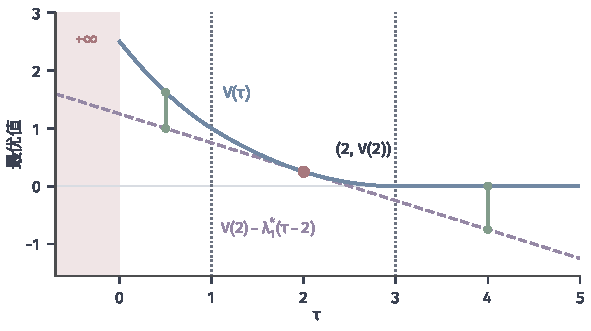
\includegraphics[width=100mm]{figures/05-optimization/06-constrained-optimization/matplotlib/sens-global-bound/figure.pdf}
 \caption{预算例的最优值函数（蓝线）和由$\tau=2$处乘子$\lambda_1^\star=1/2$给出的下界（紫色虚线）。红点是基准点，绿色线段是$\tau=0.5$和$\tau=4$处下界的余量，灰色点线标出活动约束改变的$\tau=1,3$。红色区域$\tau<0$不可行，$V=+\infty$。}
 \label{fig:sens-global-bound}
\end{BookInlineFigure}

\paragraph{去掉强对偶会怎样}
强对偶达到这个条件不能换成“存在KKT乘子”。考虑非凸问题
\[
 \min_{x\in\mathbb{R}}\ -x^2\quad\text{s.t.}\quad x-1\leq u,\ \ -x-1\leq0.
\]
基准问题$u=0$的可行集是$[-1,1]$，$f^\star=-1$，在$x=\pm1$取得。

在$x=1$处，平稳条件$-2x+\lambda_1=0$给出KKT乘子$\lambda_1=2$，第二条约束不起作用，$\lambda_2=0$。如果照搬式~\eqref{eq:sens-rhs-bound}，会得到$V(u)\geq-1-2u$。

直接计算最优值。$u>0$时可行集是$[-1,1+u]$，最小点在$x=1+u$。$-2\leq u\leq0$时，可行集右端点的绝对值不超过$1$，最小点在$x=-1$。所以
\[
 V(u)=\begin{cases}-1,&-2\leq u\leq0,\\-(1+u)^2,&u>0.\end{cases}
\]
$u>0$时，
\[
 V(u)-(-1-2u)=-u^2<0,
\]
下界不成立，见图~\ref{fig:sens-kkt-no-bound}。原因是这个问题的对偶函数对任何乘子都是$-\infty$，强对偶不成立。KKT乘子只承载局部信息，全局下界必须由对偶最优的乘子给出。

\begin{BookInlineFigure}
 \centering
 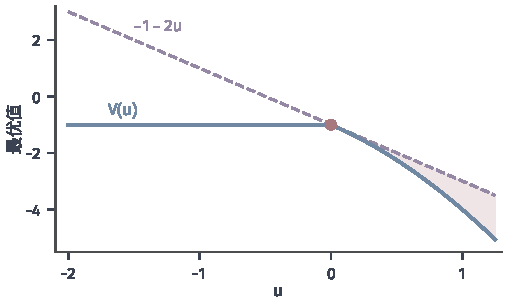
\includegraphics[width=86mm]{figures/05-optimization/06-constrained-optimization/matplotlib/sens-kkt-no-bound/figure.pdf}
 \caption{KKT乘子不给出全局下界的例子。蓝线是$\min-x^2$，$x-1\leq u$，$x\geq-1$的最优值$V(u)$，紫色虚线是用$x=1$处KKT乘子$2$写出的直线$-1-2u$，红色区域表示$u>0$时直线高于$V$。}
 \label{fig:sens-kkt-no-bound}
\end{BookInlineFigure}

非凸并不一定导致失败。对问题$\min-x^2$，$x^2-1\leq u$，取$\lambda=1$，Lagrange函数恒等于$-1$，所以$q(1)=-1=f^\star$。此时$V(u)=-1-u$（$u\geq-1$），下界恰好取等号。起决定作用的是零间隙，而不是凸性。

\subsection{乘子的边际解释}
\label{sec:sens-marginal}

下界只说明$V$不低于一条直线。什么时候这条直线就是$V$的切线，乘子就是最优值的真实变化率？本小节回答这个问题。

\paragraph{直线贴着曲线时}
一条直线处处不高于曲线，又在基准点与曲线相交。如果曲线在该点光滑，直线就没有选择，只能是切线。这正是图~\ref{fig:sens-global-bound}中红点处的情形。把这个几何观察写成定理：

\begin{theorem}[乘子是边际变化率]
\label{thm:sens-marginal}
在定理~\ref{thm:sens-rhs-bound}的条件下，进一步设$V$在$(\bm{0},\bm{0})$附近有限且在$(\bm{0},\bm{0})$可微，则
\begin{equation}
 \frac{\partial V}{\partial u_i}(\bm{0},\bm{0})=-\lambda_i^\star,
 \qquad
 \frac{\partial V}{\partial v_j}(\bm{0},\bm{0})=-\nu_j^\star.
 \label{eq:sens-marginal}
\end{equation}
\end{theorem}

\begin{proof}
定义函数
\[
 \varphi(\bm{u},\bm{v})=V(\bm{u},\bm{v})-f^\star+\langle\bm{\lambda}^\star,\bm{u}\rangle+\langle\bm{\nu}^\star,\bm{v}\rangle.
\]
式~\eqref{eq:sens-rhs-bound}说明$\varphi\geq0$，而$\varphi(\bm{0},\bm{0})=0$，所以原点是$\varphi$的极小点。原点是定义域的内点，$\varphi$在原点可微，它的梯度必须为零。写出这个梯度的各个分量，就是式~\eqref{eq:sens-marginal}。
\end{proof}

定理同时说明，只要$V$在基准点可微，满足条件的乘子就是唯一的，因为它们都等于$V$的梯度的相反数。

\paragraph{几何含义}
在预算例中，$-\nabla f(\bm{x}^\star)=\lambda_1^\star(1,1)$垂直于预算线。图~\ref{fig:sens-shadow-price-geometry}中，预算增加$\Delta\tau$时，预算线沿法向平移$\Delta\tau/\sqrt{2}$。目标沿法向的变化率是
\[
 \lVert\nabla f(\bm{x}^\star)\rVert_2=\lambda_1^\star\sqrt{2}.
\]
两者相乘，目标的一阶下降量是$\lambda_1^\star\Delta\tau$，这就是乘子作为\emph{影子价格}的含义：多一单位预算大约值$\lambda_1^\star$。没有起作用的约束乘子为零，放宽它们一阶没有价值。

\begin{BookInlineFigure}
 \centering
 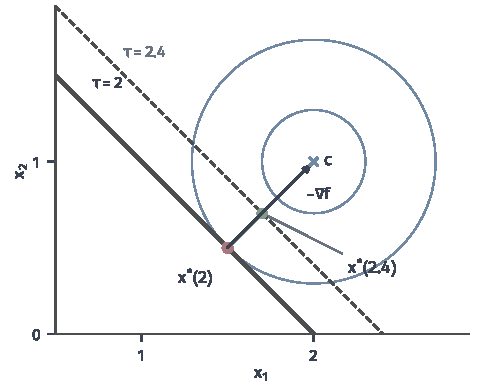
\includegraphics[width=84mm]{figures/05-optimization/06-constrained-optimization/matplotlib/sens-shadow-price-geometry/figure.pdf}
 \caption{预算线平移与乘子。深灰实线是$\tau=2$的预算线，虚线是$\tau=2.4$的预算线，蓝色圆是目标等高线。黑色箭头是$-\nabla f(\bm{x}^\star)=\lambda_1^\star(1,1)$，从红点指向理想点$\bm{c}$。绿色线段是最优解的移动。}
 \label{fig:sens-shadow-price-geometry}
\end{BookInlineFigure}

核对数值。$1<\tau<3$时，$V(\tau)=(3-\tau)^2/4$，这个公式将在第~\ref{sec:sens-active-change}节推出。于是$V'(2)=-1/2=-\lambda_1^\star$。取$\Delta\tau=0.4$，一阶估计是$0.25-0.2=0.05$，真实值$V(2.4)=0.09$。一阶估计恰好等于式~\eqref{eq:sens-budget-bound}的下界，真实值在它上方。

\paragraph{值函数不可微时}
可微性不是自动成立的。下面的引理不要求可微，并且给出了全局下界的完整刻画：所有能作全局下界斜率的向量，恰好就是全体最优乘子的相反数。

\begin{lemma}[下界斜率与最优乘子]
\label{lem:sens-support-multipliers}
设$f^\star$有限，$\bm{\lambda}\in\mathbb{R}^m$，$\bm{\nu}\in\mathbb{R}^p$，$f,g_i,h_j$定义在同一集合$\bm{D}$上，式~\eqref{eq:sens-rhs-value}及对偶函数中的$\bm{x}$都取遍$\bm{D}$。则下面两条等价：
\begin{enumerate}
 \item $\bm{\lambda}\geq\bm{0}$，且$q(\bm{\lambda},\bm{\nu})=f^\star$；
 \item 对所有$(\bm{u},\bm{v})$，都有
 \begin{equation}
  V(\bm{u},\bm{v})\geq f^\star-\langle\bm{\lambda},\bm{u}\rangle-\langle\bm{\nu},\bm{v}\rangle.
  \label{eq:sens-support}
 \end{equation}
\end{enumerate}
\end{lemma}

\begin{proof}
第一条推出第二条，这就是定理~\ref{thm:sens-rhs-bound}。下面从第二条出发。先证明$\lambda_i\geq0$。取$t>0$，令$\bm{u}=t\bm{e}_i$，$\bm{v}=\bm{0}$。放宽约束只会扩大可行集，所以$V(t\bm{e}_i,\bm{0})\leq f^\star$。结合式~\eqref{eq:sens-support}，得到
\[
 f^\star\geq V(t\bm{e}_i,\bm{0})\geq f^\star-t\lambda_i.
\]
所以$\lambda_i\geq0$。

再证明$q(\bm{\lambda},\bm{\nu})\geq f^\star$。任取$\bm{x}\in\bm{D}$，令$u_i=g_i(\bm{x})$，$v_j=h_j(\bm{x})$。这个$\bm{x}$是这组扰动问题的可行点，所以$f(\bm{x})\geq V(\bm{u},\bm{v})$。再由式~\eqref{eq:sens-support}，
\[
 f(\bm{x})\geq f^\star-\sum_i\lambda_ig_i(\bm{x})-\sum_j\nu_jh_j(\bm{x}).
\]

移项得到
\[
 \mathcal{L}(\bm{x},\bm{\lambda},\bm{\nu})\geq f^\star.
\]
对$\bm{x}$取下确界，得到$q(\bm{\lambda},\bm{\nu})\geq f^\star$。又由弱对偶$q(\bm{\lambda},\bm{\nu})\leq f^\star$，所以两者相等。
\end{proof}

当$f$与$g_i$是凸函数、$h_j$是仿射函数时，$V$是凸函数。取两组扰动及各自的近优可行点，它们的凸组合对扰动的相应凸组合仍可行，目标值不超过相应的凸组合，由此就得到$V$的凸性。

这时式~\eqref{eq:sens-support}正是第~\ref{chap:nonsmooth-composite-optimization}章次梯度的定义，引理说的就是$-(\bm{\lambda},\bm{\nu})$属于$V$在原点的次微分。若原点还是$V$的定义域的内点，$V$在方向$(\bm{u},\bm{v})$上的方向导数等于
\begin{equation}
 V'\bigl(\bm{0},\bm{0};\bm{u},\bm{v}\bigr)=\max_{(\bm{\lambda},\bm{\nu})\ \text{最优}}\bigl(-\langle\bm{\lambda},\bm{u}\rangle-\langle\bm{\nu},\bm{v}\rangle\bigr),
 \label{eq:sens-directional}
\end{equation}
其中最大值取遍全部最优乘子。这个等式的证明需要用到凸函数方向导数与次微分的对偶关系，篇幅较长，读者可查阅\scite{rockafellar1970convex}。它的含义是：每个方向上的真实变化率由“最不利”的乘子决定，单独一组乘子不能代表所有方向。

\paragraph{一个有折角的例子}
考虑一维问题
\[
 \min_{x\in\mathbb{R}}\ -x\quad\text{s.t.}\quad x-1\leq u,\ \ x-1\leq0.
\]
两条约束在$u=0$时完全相同，$x^\star=1$，$f^\star=-1$。Lagrange函数是
\[
 \mathcal{L}(x,\bm{\lambda})=(-1+\lambda_1+\lambda_2)x-\lambda_1-\lambda_2.
\]

$\lambda_1+\lambda_2\neq1$时它对$x$无下界。$\lambda_1+\lambda_2=1$时它恒等于$-1$。所以最优乘子集合是线段$\{\bm{\lambda}\geq\bm{0}:\lambda_1+\lambda_2=1\}$，乘子不唯一。

右端扰动的最优值可以直接写出。$u\geq0$时第二条约束决定解，$x=1$；$u<0$时第一条约束决定解，$x=1+u$。所以
\[
 V(u)=\max\{-1-u,\ -1\}.
\]

$V$在$u=0$处有折角，左导数是$-1$，右导数是$0$。图~\ref{fig:sens-subgrad-kink}(a)中斜率在$[-1,0]$内的每条直线都是全局下界，它们恰好对应(b)中线段上的每个乘子。

由式~\eqref{eq:sens-directional}，向右的方向导数$V'(0;1)=\max(-\lambda_1)=0$，由$\lambda_1=0$取到。向左的方向导数$V'(0;-1)=\max\lambda_1=1$，由$\lambda_1=1$取到。求解器如果返回对称的乘子$(1/2,1/2)$，那么$-1/2$只是一个合法的下界斜率，不是任何方向上的导数。

\begin{BookInlineFigure}
 \centering
 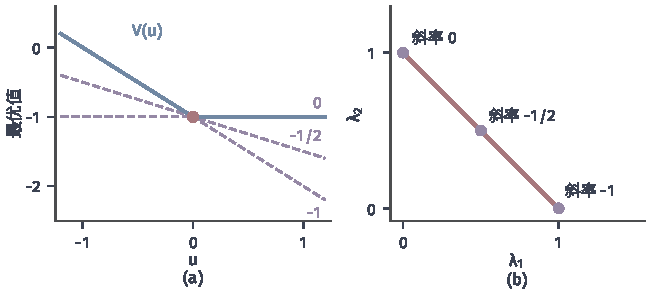
\includegraphics[width=112mm]{figures/05-optimization/06-constrained-optimization/matplotlib/sens-subgrad-kink/figure.pdf}
 \caption{乘子不唯一时的值函数。(a)~蓝线是$V(u)=\max\{-1-u,-1\}$，紫色虚线是斜率$0,-1/2,-1$的全局下界，它们都穿过红点。(b)~红色线段是全体最优乘子，紫色点是图(a)三条直线对应的乘子。}
 \label{fig:sens-subgrad-kink}
\end{BookInlineFigure}

表~\ref{tab:sens-three-slopes}比较本节出现的三个量。

\begin{BookInlineTable}
 \centering
 \begin{tabular}{lll}
  \toprule
  对象 & 成立条件 & 范围\\
  \midrule
  下界斜率$-\bm{\lambda}^\star$ & 零间隙且乘子达到 & 全局，单侧\\
  实际导数$-\bm{\lambda}^\star$ & 另加$V$在基准点可微 & 局部，一阶\\
  方向导数 & 凸问题、基准点在定义域内部 & 局部，沿给定方向\\
  \bottomrule
 \end{tabular}
 \caption{约束右端扰动下的三个量。下界斜率来自任何一组最优乘子，实际导数要求$V$可微，方向导数要在全体最优乘子上取最大值。}
 \label{tab:sens-three-slopes}
\end{BookInlineTable}

\subsection{目标参数的包络关系}
\label{sec:sens-envelope}

现在让目标函数含参数，可行集固定。最优解随参数移动，所以最优值的变化似乎有两个来源：目标本身变了，最优点也动了。本小节的结论是，一阶意义下第二个来源不起作用。

\paragraph{谷底的一阶平坦}
站在谷底，向任何方向走一小步，高度的一阶变化都是零。最优解被参数推着移动一小段，走的正是这样的一小步，所以高度的变化几乎全部来自地形本身的改变。这是整个包络关系的直观基础。

在边界上情况稍有不同：梯度不必为零，因为有约束挡住。但如果解沿着边界来回移动，它向两个相反的方向都是可行的，梯度只能与这个移动方向垂直。

\begin{theorem}[包络关系]
\label{thm:sens-envelope}
设$\bm{C}\subseteq\mathbb{R}^n$固定，$f$在$(\bm{x}_0,\bm{\theta}_0)$的邻域内连续可微。设映射$\bm{x}(\cdot)$定义在$\bm{\theta}_0$的邻域上，取值于$\bm{C}$，在$\bm{\theta}_0$处可微，$\bm{x}(\bm{\theta}_0)=\bm{x}_0$，且$\bm{x}_0$是$f(\cdot,\bm{\theta}_0)$在$\bm{C}$上的局部极小点。记$v$为式~\eqref{eq:sens-branch-value}定义的分支值，则
\begin{equation}
 \nabla v(\bm{\theta}_0)=\nabla_{\bm{\theta}}f(\bm{x}_0,\bm{\theta}_0).
 \label{eq:sens-envelope}
\end{equation}
\end{theorem}

\begin{proof}
记$\bm{D}_{\bm{x}}\in\mathbb{R}^{n\times q}$是$\bm{x}(\cdot)$在$\bm{\theta}_0$的Jacobian矩阵。由链式法则，
\[
 \nabla v(\bm{\theta}_0)=\nabla_{\bm{\theta}}f(\bm{x}_0,\bm{\theta}_0)+\bm{D}_{\bm{x}}^{\top}\nabla_{\bm{x}}f(\bm{x}_0,\bm{\theta}_0).
\]
只需证明第二项为零。任取方向$\bm{d}\in\mathbb{R}^q$，令
\[
 \psi(t)=f\bigl(\bm{x}(\bm{\theta}_0+t\bm{d}),\bm{\theta}_0\bigr).
\]

注意$\psi$里的参数固定在$\bm{\theta}_0$。$\lvert t\rvert$很小时，$\bm{x}(\bm{\theta}_0+t\bm{d})$属于$\bm{C}$且靠近$\bm{x}_0$，所以$\psi(t)\geq\psi(0)$。$t=0$是$\psi$的内部极小点，$\psi'(0)=0$，也就是
\[
 \bigl\langle\nabla_{\bm{x}}f(\bm{x}_0,\bm{\theta}_0),\ \bm{D}_{\bm{x}}\bm{d}\bigr\rangle=0.
\]
$\bm{d}$是任意的，所以
\[
 \bm{D}_{\bm{x}}^{\top}\nabla_{\bm{x}}f(\bm{x}_0,\bm{\theta}_0)=\bm{0}.
\]
\end{proof}

结论说的是分支上的值$v$，而不是全局最优值$V$。条件里最关键的是$\bm{C}$固定：这样分支上的点对基准问题仍是可行的，才能用基准点的局部极小性。约束也含参数的情形放在第~\ref{sec:sens-general-constraints}节。

\paragraph{预算例：理想点移动}
把理想点改成$(2+\theta,1)$，预算固定为$\tau=2$，目标是
\[
 f(\bm{x},\theta)=\frac12(x_1-2-\theta)^2+\frac12(x_2-1)^2.
\]
$\lvert\theta\rvert<1$时只有预算起作用。平稳条件是$x_1-2-\theta+\lambda=0$、$x_2-1+\lambda=0$，与$x_1+x_2=2$联立，得到
\[
 \lambda=\frac{1+\theta}{2},\qquad
 x_1(\theta)=\frac32+\frac{\theta}{2},\qquad
 x_2(\theta)=\frac12-\frac{\theta}{2}.
\]

分支上的值是$v(\theta)=\lambda^2=(1+\theta)^2/4$，直接求导得到$v'(\theta)=(1+\theta)/2$。用包络关系，只需对目标中显含的$\theta$求偏导：
\[
 \frac{\partial f}{\partial\theta}=2+\theta-x_1=\frac{1+\theta}{2}.
\]
两个结果一致。解的移动方向是$\bm{x}'(\theta)=(1/2,-1/2)$，$\nabla_{\bm{x}}f=-\lambda(1,1)$，两者的内积确实为零。图~\ref{fig:sens-envelope}(a)显示，解沿预算线滑动，而负梯度垂直于这条线。

\paragraph{为什么叫包络}
把决策$\hat{\bm{x}}$固定，$\theta\mapsto f(\hat{\bm{x}},\theta)$就是一条曲线。每个固定的决策对应一条这样的曲线，它们都在$v(\theta)$上方，因为固定决策不会比最优决策好。图~\ref{fig:sens-envelope}(b)中$v$是这族曲线的下边缘，称为它们的\emph{包络}，式~\eqref{eq:sens-envelope}因此称为\term{包络定理}（envelope theorem）。

曲线在切点处与$v$相切。切点处的斜率既是这条固定决策曲线的斜率，也是$v$的斜率，这正是“只对显含的$\theta$求导”的图形含义。

\begin{BookInlineFigure}
 \centering
 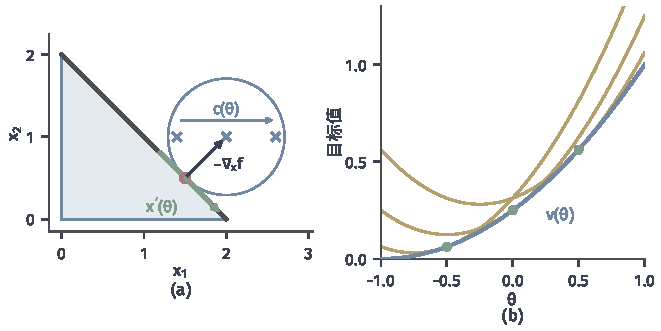
\includegraphics[width=112mm]{figures/05-optimization/06-constrained-optimization/matplotlib/sens-envelope/figure.pdf}
 \caption{包络关系。(a)~$\tau=2$的可行集上，理想点沿蓝色箭头移动（蓝色叉是$\theta=-0.6,0,0.6$），最优解沿绿色线段滑动。红点是$\theta=0$的解，黑色箭头是负梯度，绿色箭头是解的移动方向，两者垂直。(b)~黄线是把决策固定在$\theta=-0.5,0,0.5$的最优解上得到的目标值，蓝线$v(\theta)$是它们的下边缘，绿点是切点。}
 \label{fig:sens-envelope}
\end{BookInlineFigure}

\paragraph{没有可微分支时}
定理~\ref{thm:sens-envelope}需要一条可微的解分支。若最优解不唯一，或最优解随参数跳动，这样的分支就没有了。但只要可行集紧，全局最优值的方向导数仍然有公式，这就是Danskin型结果。

\begin{theorem}[Danskin型结果]
\label{thm:sens-danskin}
设$\bm{C}\subseteq\mathbb{R}^n$非空且紧，$\bm{\Theta}\subseteq\mathbb{R}^q$开，$f$在$\bm{C}\times\bm{\Theta}$上连续，关于$\bm{\theta}$的梯度$\nabla_{\bm{\theta}}f$存在且在$\bm{C}\times\bm{\Theta}$上连续。记$V$为式~\eqref{eq:sens-value}在$\bm{C}(\bm{\theta})\equiv\bm{C}$时的最优值函数，则对每个$\bm{\theta}\in\bm{\Theta}$与方向$\bm{d}$，
\begin{equation}
 V'(\bm{\theta};\bm{d})=\min_{\bm{x}\in\bm{S}(\bm{\theta})}\bigl\langle\nabla_{\bm{\theta}}f(\bm{x},\bm{\theta}),\bm{d}\bigr\rangle.
 \label{eq:sens-danskin}
\end{equation}
若$\bm{S}(\bm{\theta})=\{\bm{x}^\star\}$只有一个点，则$V$在$\bm{\theta}$可微，且
\begin{equation}
 \nabla V(\bm{\theta})=\nabla_{\bm{\theta}}f(\bm{x}^\star,\bm{\theta}).
 \label{eq:sens-danskin-gradient}
\end{equation}
\end{theorem}

\begin{proof}
$\bm{S}(\bm{\theta})$是紧集$\bm{C}$的闭子集，所以式~\eqref{eq:sens-danskin}的最小值可以取到。下面从两个方向夹逼。

先证上界。任取$\bm{x}\in\bm{S}(\bm{\theta})$和$t>0$。$\bm{x}$对$\bm{\theta}+t\bm{d}$仍可行，而且在$\bm{\theta}$处最优，所以
\[
 V(\bm{\theta}+t\bm{d})\leq f(\bm{x},\bm{\theta}+t\bm{d}),\qquad V(\bm{\theta})=f(\bm{x},\bm{\theta}).
\]
由一元中值定理，存在$\xi\in(0,1)$，使
\[
 \frac{V(\bm{\theta}+t\bm{d})-V(\bm{\theta})}{t}\leq\bigl\langle\nabla_{\bm{\theta}}f(\bm{x},\bm{\theta}+\xi t\bm{d}),\bm{d}\bigr\rangle.
\]
令$t\downarrow0$，由梯度的连续性，上极限不超过$\langle\nabla_{\bm{\theta}}f(\bm{x},\bm{\theta}),\bm{d}\rangle$。再对$\bm{x}\in\bm{S}(\bm{\theta})$取最小，就得到上界。

再证下界。取$t_k\downarrow0$，使差商趋于它的下极限，并取$\bm{x}_k\in\bm{S}(\bm{\theta}+t_k\bm{d})$。$\bm{C}$是紧集，可以取子列使$\bm{x}_k\to\bar{\bm{x}}\in\bm{C}$。对任意$\bm{y}\in\bm{C}$，$\bm{x}_k$的最优性给出
\[
 f(\bm{x}_k,\bm{\theta}+t_k\bm{d})\leq f(\bm{y},\bm{\theta}+t_k\bm{d}).
\]
令$k\to\infty$并用$f$的连续性，可知$\bar{\bm{x}}$在参数$\bm{\theta}$下的目标值不超过任何$\bm{y}\in\bm{C}$的目标值，所以$\bar{\bm{x}}\in\bm{S}(\bm{\theta})$。

此外，$\bm{x}_k$是基准问题的可行点，又在$\bm{\theta}+t_k\bm{d}$处最优，所以
\[
 V(\bm{\theta})\leq f(\bm{x}_k,\bm{\theta}),\qquad V(\bm{\theta}+t_k\bm{d})=f(\bm{x}_k,\bm{\theta}+t_k\bm{d}).
\]
再用一次中值定理，存在$\xi_k\in(0,1)$，使
\[
 \frac{V(\bm{\theta}+t_k\bm{d})-V(\bm{\theta})}{t_k}\geq\bigl\langle\nabla_{\bm{\theta}}f(\bm{x}_k,\bm{\theta}+\xi_kt_k\bm{d}),\bm{d}\bigr\rangle.
\]
令$k\to\infty$，下极限不小于$\langle\nabla_{\bm{\theta}}f(\bar{\bm{x}},\bm{\theta}),\bm{d}\rangle$，它又不小于式~\eqref{eq:sens-danskin}的右端。上下界合起来，方向导数存在并等于右端。

只有一个解时，把上面两步中的$t\bm{d}$换成趋于零的向量$\bm{\delta}$。上界一步给出
\[
 V(\bm{\theta}+\bm{\delta})-V(\bm{\theta})\leq\langle\nabla_{\bm{\theta}}f(\bm{x}^\star,\bm{\theta}),\bm{\delta}\rangle+o(\lVert\bm{\delta}\rVert_2).
\]
下界一步中$\bm{x}_{\bm{\delta}}\to\bm{x}^\star$，因为任何极限点都属于单点集$\bm{S}(\bm{\theta})$，于是相同的表达式也是下界。所以$V$可微。
\end{proof}

式~\eqref{eq:sens-danskin}取的是最小值，这与目标是最小化相对应。直观上，参数沿$\bm{d}$变化时，全部最优解处在同一起跑线上，下一时刻仍然留在最优的，是在方向$\bm{d}$上目标增长最慢的那一个。

\paragraph{条件的作用：多解时的方向导数}
考虑线性目标$f(\bm{x},p)=-px_1-x_2$，可行集是$\tau=2$的三角形。$p>1$时最优点是$(2,0)$，$p<1$时最优点是$(0,2)$，$p=1$时整条预算线都是最优解，见图~\ref{fig:sens-danskin-edge}。最优值是
\[
 V(p)=-2\max\{p,1\}.
\]

在$p=1$处，$\partial f/\partial p=-x_1$。式~\eqref{eq:sens-danskin}给出
\[
 V'(1;1)=\min_{\bm{x}\in\bm{S}(1)}(-x_1)=-2,\qquad
 V'(1;-1)=\min_{\bm{x}\in\bm{S}(1)}x_1=0.
\]
第一个由顶点$(2,0)$取到，第二个由顶点$(0,2)$取到，与图中两段的斜率一致。

\begin{BookInlineFigure}
 \centering
 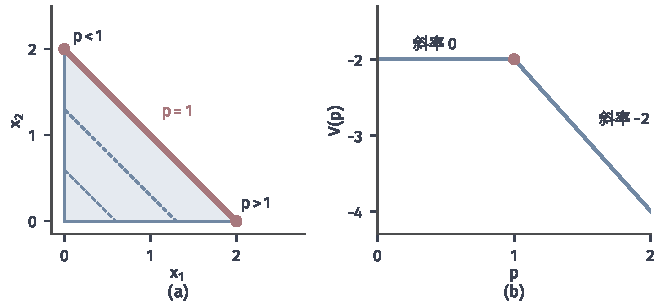
\includegraphics[width=112mm]{figures/05-optimization/06-constrained-optimization/matplotlib/sens-danskin-edge/figure.pdf}
 \caption{线性目标$-px_1-x_2$在三角形$x_1+x_2\leq2$，$\bm{x}\geq\bm{0}$上的最优解。(a)~$p=1$时蓝色虚线的等值线平行于预算线，红色粗线上的点都最优；$p>1$或$p<1$时解是相应的红色顶点。(b)~最优值$V(p)=-2\max\{p,1\}$在$p=1$有折角。}
 \label{fig:sens-danskin-edge}
\end{BookInlineFigure}

紧性不能随意去掉。第~\ref{sec:sens-problems}节的$f(x,\theta)=e^x-\theta x$在$\theta=0$处没有最优解，式~\eqref{eq:sens-danskin}的右端失去意义。实际上$\theta>0$时$V(\theta)=\theta-\theta\ln\theta$，所以
\[
 \frac{V(\theta)-V(0)}{\theta}=1-\ln\theta\to+\infty\quad(\theta\downarrow0),
\]
$V$在$\theta=0$处的右导数不是有限数。

\subsection{一般含参约束}
\label{sec:sens-general-constraints}

现在目标和约束都含参数。可行集随参数移动，上一小节的证明不能直接用，因为分支上的点对基准问题已经不可行。本小节说明，对沿分支的值求导时，Lagrange函数吸收了约束移动的贡献。

\paragraph{从目标到Lagrange函数}
考虑一族问题
\begin{equation}
 \min_{\bm{x}}\ f(\bm{x},\bm{\theta})\quad
 \text{s.t.}\quad g_i(\bm{x},\bm{\theta})\leq0,\ \ h_j(\bm{x},\bm{\theta})=0,
 \label{eq:sens-general-problem}
\end{equation}
其Lagrange函数$\mathcal{L}(\bm{x},\bm{\lambda},\bm{\nu},\bm{\theta})$也含参数。下面的定理假设已经有一条KKT点分支，并且起作用的约束保持起作用。这条分支从何而来，由第~\ref{sec:sens-solution}节回答。

\begin{theorem}[分支值对参数的导数]
\label{thm:sens-general-branch}
设$f,g_i,h_j$在$(\bm{x}_0,\bm{\theta}_0)$的邻域内连续可微。设映射$\bm{x}(\cdot)$在$\bm{\theta}_0$的邻域上满足$\bm{x}(\bm{\theta}_0)=\bm{x}_0$，在$\bm{\theta}_0$可微，$(\bm{x}_0,\bm{\lambda}_0,\bm{\nu}_0)$在$\bm{\theta}_0$处满足平稳条件，且沿分支恒有
\begin{equation}
 g_i(\bm{x}(\bm{\theta}),\bm{\theta})=0\ \ (\lambda_{0,i}>0),\qquad
 h_j(\bm{x}(\bm{\theta}),\bm{\theta})=0.
 \label{eq:sens-active-held}
\end{equation}
记$v$为式~\eqref{eq:sens-branch-value}定义的分支值，则
\begin{equation}
 \nabla v(\bm{\theta}_0)=\nabla_{\bm{\theta}}\mathcal{L}(\bm{x}_0,\bm{\lambda}_0,\bm{\nu}_0,\bm{\theta}_0).
 \label{eq:sens-general-gradient}
\end{equation}
\end{theorem}

\begin{proof}
下面所有函数都在$(\bm{x}_0,\bm{\theta}_0)$取值，$\bm{D}_{\bm{x}}$是分支的Jacobian矩阵。由链式法则，
\[
 \nabla v=\nabla_{\bm{\theta}}f+\bm{D}_{\bm{x}}^{\top}\nabla_{\bm{x}}f.
\]
用平稳条件替换$\nabla_{\bm{x}}f$，乘子为零的项自动消失：
\[
 \bm{D}_{\bm{x}}^{\top}\nabla_{\bm{x}}f=-\sum_{i}\lambda_{0,i}\bm{D}_{\bm{x}}^{\top}\nabla_{\bm{x}}g_i-\sum_j\nu_{0,j}\bm{D}_{\bm{x}}^{\top}\nabla_{\bm{x}}h_j.
\]

对恒等式$g_i(\bm{x}(\bm{\theta}),\bm{\theta})=0$求导，得到
\[
 \bm{D}_{\bm{x}}^{\top}\nabla_{\bm{x}}g_i+\nabla_{\bm{\theta}}g_i=\bm{0}.
\]
等式约束同样如此。代回上一式，得到
\[
 \bm{D}_{\bm{x}}^{\top}\nabla_{\bm{x}}f=\sum_i\lambda_{0,i}\nabla_{\bm{\theta}}g_i+\sum_j\nu_{0,j}\nabla_{\bm{\theta}}h_j.
\]
加上$\nabla_{\bm{\theta}}f$，右端就是$\nabla_{\bm{\theta}}\mathcal{L}$。
\end{proof}

式~\eqref{eq:sens-general-gradient}包含两部分贡献。$\nabla_{\bm{\theta}}f$是目标本身的变化，$\sum\lambda_i\nabla_{\bm{\theta}}g_i$是约束移动造成的变化，乘子把约束的移动折算成目标的变化。若约束不含参数，第二部分为零，回到包络关系。若$g_1=x_1+x_2-\tau$，则$\partial g_1/\partial\tau=-1$，式~\eqref{eq:sens-general-gradient}给出$v'(\tau)=-\lambda_1$，回到边际解释。

\paragraph{一个目标与约束同时含参的例子}
让参数$\theta$同时影响目标和预算的价格：
\[
 \min_{\bm{x}}\ \frac12(x_1-1-\theta)^2+\frac12(x_2-1)^2
 \quad\text{s.t.}\quad \theta x_1+x_2-2\leq0.
\]
$\theta=1$时它就是$\tau=2$的预算例。$\theta$变大时，第一种投入的单价上涨，预算线绕$(0,2)$转动，理想点也同时右移，见图~\ref{fig:sens-moving-constraint}。

\begin{BookInlineFigure}
 \centering
 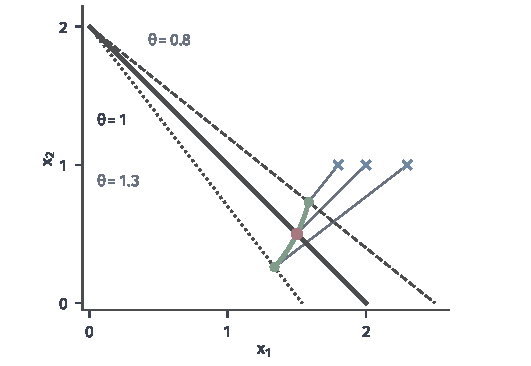
\includegraphics[width=90mm]{figures/05-optimization/06-constrained-optimization/matplotlib/sens-moving-constraint/figure.pdf}
 \caption{目标与约束同时含参。三条深灰线是$\theta=0.8,1,1.3$的预算线$\theta x_1+x_2=2$，蓝色叉是相应的理想点$(1+\theta,1)$，细灰线连接理想点和最优解。绿色曲线是最优解随$\theta$的路径，红点是$\theta=1$的解。}
 \label{fig:sens-moving-constraint}
\end{BookInlineFigure}

预算约束起作用时，平稳条件是$x_1-1-\theta+\lambda\theta=0$、$x_2-1+\lambda=0$。把$x_1=1+\theta-\lambda\theta$与$x_2=1-\lambda$代入$\theta x_1+x_2=2$，解出
\[
 \lambda(\theta)=\frac{\theta^2+\theta-1}{1+\theta^2}.
\]
$\theta=1$时$\lambda=1/2$，$\bm{x}=(3/2,1/2)$。

用式~\eqref{eq:sens-general-gradient}，目标与约束的偏导数分别是
\[
 \frac{\partial f}{\partial\theta}=-(x_1-1-\theta)=\lambda\theta=\frac12,
 \qquad
 \lambda\frac{\partial g}{\partial\theta}=\lambda x_1=\frac34.
\]
相加得到$v'(1)=5/4$。目标的直接变化贡献$1/2$，价格上涨使约束收紧，贡献$3/4$。

直接核对：把解代入目标，得到$v(\theta)=\tfrac12\lambda^2(1+\theta^2)$，即
\[
 v(\theta)=\frac{(\theta^2+\theta-1)^2}{2(1+\theta^2)}.
\]
在$\theta=1$处求导，分子$N=\theta^2+\theta-1$满足$N=1$，$N'=3$，分母$D=1+\theta^2$满足$D=2$，$D'=2$，所以
\[
 v'(1)=\frac{NN'}{D}-\frac{N^2D'}{2D^2}=\frac32-\frac14=\frac54.
\]
两个结果一致。式~\eqref{eq:sens-general-gradient}不需要先解出分支，只需要基准点的$\bm{x}$和乘子。

\section{最优解的变化}
\label{sec:sens-solution}

最优值是一个数，最优解是一个向量，后者需要更多的结构才能求导。这就需要回答：选定一个解之后，它随参数怎样移动？办法是把这个解满足的最优性条件看成一组方程，方程里既有原变量和乘子，也有参数，然后像解隐函数那样求局部导数。

\paragraph{隐函数定理的回顾}
所用的工具是隐函数定理：设$\bm{F}(\bm{z},\bm{\theta})$连续可微，$\bm{F}(\bm{z}_0,\bm{\theta}_0)=\bm{0}$，方阵$\bm{D}_{\bm{z}}\bm{F}(\bm{z}_0,\bm{\theta}_0)$可逆。则在$\bm{\theta}_0$附近有唯一的连续可微映射$\bm{z}(\bm{\theta})$，使$\bm{z}(\bm{\theta}_0)=\bm{z}_0$，且在$(\bm{z}_0,\bm{\theta}_0)$的某个邻域内方程的解全部落在这条曲线上。它的导数满足线性方程
\[
 \bm{D}_{\bm{z}}\bm{F}\cdot\bm{D}\bm{z}=-\bm{D}_{\bm{\theta}}\bm{F}.
\]
定理的陈述与证明可参考\BookChapterRef{chap:implicit-inverse-functions}{卷二第22章“隐函数与反函数”}。

用它研究极小点时要多一步检查，因为隐函数定理只管方程。例如$f(x,\theta)=-x^2/2+\theta x$的驻点方程是$-x+\theta=0$，导数$-1$可逆，隐函数定理给出光滑分支$x(\theta)=\theta$，而这条分支上全是极大点。所以下面每个定理都分成两部分：方程有光滑解，以及这个解确实是极小点。

\subsection{无约束极小解}
\label{sec:sens-unconstrained}

\paragraph{碗的曲率决定碗底移动的距离}
无约束时，$\bm{x}^\star$是碗底，满足$\nabla_{\bm{x}}f=\bm{0}$。参数一变，梯度在原来的位置上不再为零，碗底要移动到新的梯度零点。线性近似告诉我们移动多少：
\[
 \nabla^2_{\bm{x}\bm{x}}f\cdot\Delta\bm{x}+\nabla^2_{\bm{x}\bm{\theta}}f\cdot\Delta\bm{\theta}\approx\bm{0}.
\]
曲率大的方向，碗壁陡，碗底只需移动一点就能抵消参数带来的梯度变化；曲率小的方向，碗底要移动很远。

\begin{theorem}[无约束极小解的导数]
\label{thm:sens-unconstrained}
设$f$在$(\bm{x}_0,\bm{\theta}_0)$的邻域内二阶连续可微，$\nabla_{\bm{x}}f(\bm{x}_0,\bm{\theta}_0)=\bm{0}$，$\nabla^2_{\bm{x}\bm{x}}f(\bm{x}_0,\bm{\theta}_0)\succ\bm{0}$。则存在$\bm{\theta}_0$的邻域和唯一的连续可微映射$\bm{x}(\cdot)$，使$\bm{x}(\bm{\theta}_0)=\bm{x}_0$，且邻域内的每个$\bm{x}(\bm{\theta})$都是$f(\cdot,\bm{\theta})$的严格局部极小点。Jacobian矩阵$\bm{D}_{\bm{x}}\in\mathbb{R}^{n\times q}$由线性方程
\begin{equation}
 \nabla^2_{\bm{x}\bm{x}}f\cdot\bm{D}_{\bm{x}}=-\nabla^2_{\bm{x}\bm{\theta}}f
 \label{eq:sens-unconstrained-derivative}
\end{equation}
确定，其中各导数都在$(\bm{x}(\bm{\theta}),\bm{\theta})$处取值。
\end{theorem}

\begin{proof}
令$\bm{F}=\nabla_{\bm{x}}f$。$f$二阶连续可微，所以$\bm{F}$连续可微。$\bm{D}_{\bm{x}}\bm{F}=\nabla^2_{\bm{x}\bm{x}}f$在基准点正定，因而可逆。隐函数定理给出连续可微的分支$\bm{x}(\bm{\theta})$，对恒等式$\bm{F}(\bm{x}(\bm{\theta}),\bm{\theta})=\bm{0}$求导就得到式~\eqref{eq:sens-unconstrained-derivative}。

再说明它是极小点。Hessian矩阵连续依赖于$(\bm{x},\bm{\theta})$，矩阵的最小特征值连续，所以$\bm{\theta}$靠近$\bm{\theta}_0$时，$\nabla^2_{\bm{x}\bm{x}}f(\bm{x}(\bm{\theta}),\bm{\theta})$仍然正定。驻点处Hessian正定，由第~\ref{chap:smooth-foundations}章的二阶充分条件，$\bm{x}(\bm{\theta})$是严格局部极小点。
\end{proof}

定理是局部的，Hessian正定只说明这条分支是局部极小，它不保证全局最优。正定性也不能减弱成可逆：上面驻点是极大点的例子中，Hessian可逆但负定。

\paragraph{例子：带二次惩罚的最小二乘}
取$\bm{A}$和$\bm{b}$如下，并用$\gamma>0$作正则系数：
\[
 \bm{A}=\begin{bmatrix}1&1\\1&0\end{bmatrix},\qquad
 \bm{b}=\begin{bmatrix}2\\0\end{bmatrix},\qquad
 f(\bm{x},\gamma)=\frac12\lVert\bm{A}\bm{x}-\bm{b}\rVert_2^2+\frac{\gamma}{2}\lVert\bm{x}\rVert_2^2.
\]
梯度为零的方程是$\bm{H}(\gamma)\bm{x}=\bm{A}^{\top}\bm{b}$，其中
\[
 \bm{H}(\gamma)=\bm{A}^{\top}\bm{A}+\gamma\bm{I}=\begin{bmatrix}2+\gamma&1\\1&1+\gamma\end{bmatrix},\qquad
 \bm{A}^{\top}\bm{b}=\begin{bmatrix}2\\2\end{bmatrix}.
\]

$\gamma>0$时$\bm{H}(\gamma)$正定，所以全局最优解存在且唯一，条件满足。在$\gamma=1$处，求$\bm{H}$的逆矩阵，得到
\[
 \bm{H}(1)=\begin{bmatrix}3&1\\1&2\end{bmatrix},\qquad
 \bm{H}(1)^{-1}=\frac15\begin{bmatrix}2&-1\\-1&3\end{bmatrix},\qquad
 \bm{x}(1)=\begin{bmatrix}2/5\\4/5\end{bmatrix}.
\]

梯度$\bm{H}(\gamma)\bm{x}-\bm{A}^{\top}\bm{b}$对$\gamma$的偏导数是$\bm{x}$本身。于是式~\eqref{eq:sens-unconstrained-derivative}给出
\[
 \bm{x}'(1)=-\bm{H}(1)^{-1}\bm{x}(1)=\begin{bmatrix}0\\-2/5\end{bmatrix}.
\]

$\gamma$增大时，解在这一点上只往$x_2$减小的方向移动，$x_1$的一阶变化恰好为零。显式解是
\[
 x_1(\gamma)=\frac{2\gamma}{1+3\gamma+\gamma^2},\qquad
 x_2(\gamma)=\frac{2+2\gamma}{1+3\gamma+\gamma^2},
\]
直接求导可以验证同一结果，$x_1(\gamma)$恰在$\gamma=1$达到最大。

\paragraph{局部导数与有限跳变}
一阶预测$\bm{x}(1)+(\gamma-1)\bm{x}'(1)$的可信范围是有限的。$\gamma=1.1$时，真解和预测分别是
\[
 \bm{x}(1.1)\approx(0.3993,\ 0.7623),\qquad
 \bm{x}(1)+0.1\,\bm{x}'(1)=(0.4,\ 0.76).
\]
两者很接近。$\gamma=3$时，真解是$(6/19,8/19)\approx(0.316,0.421)$，而预测是$(0.4,0)$，差得很远。图~\ref{fig:sens-ridge-path}显示了原因：解的路径是弯的，切线只在基准点附近贴着它。

\begin{BookInlineFigure}
 \centering
 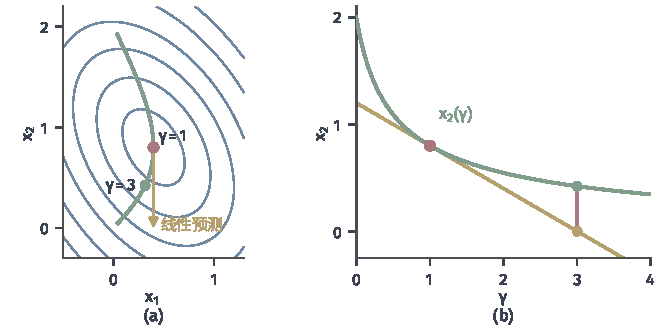
\includegraphics[width=112mm]{figures/05-optimization/06-constrained-optimization/matplotlib/sens-ridge-path/figure.pdf}
 \caption{带二次惩罚的最小二乘的解随$\gamma$的移动。(a)~蓝线是$\gamma=1$的目标等高线，绿色曲线是解的路径，红点是$\bm{x}(1)$，绿点是$\bm{x}(3)$，黄色箭头是导数给出的线性预测。(b)~$x_2(\gamma)$（绿线）与它在$\gamma=1$的切线（黄线），红色线段是$\gamma=3$处的预测误差。}
 \label{fig:sens-ridge-path}
\end{BookInlineFigure}

导数回答的是无穷小的变化。有限跳变需要另外的工具。下面的结论不需要解分支可微，对任意大小的参数差都成立。

\begin{theorem}[强凸情形的有限跳变界]
\label{thm:sens-finite-jump}
设对$\bm{\theta}\in\{\bm{\theta}_0,\bm{\theta}_1\}$，$f(\cdot,\bm{\theta})$在$\mathbb{R}^n$上可微，$\bm{x}_0$、$\bm{x}_1$分别是$f(\cdot,\bm{\theta}_0)$、$f(\cdot,\bm{\theta}_1)$的最小点，且$f(\cdot,\bm{\theta}_1)$是$\mu$强凸的。则
\begin{equation}
 \lVert\bm{x}_1-\bm{x}_0\rVert_2\leq\frac{1}{\mu}\bigl\lVert\nabla_{\bm{x}}f(\bm{x}_0,\bm{\theta}_1)-\nabla_{\bm{x}}f(\bm{x}_0,\bm{\theta}_0)\bigr\rVert_2.
 \label{eq:sens-finite-jump}
\end{equation}
\end{theorem}

\begin{proof}
强凸函数的梯度满足
\[
 \bigl\langle\nabla_{\bm{x}}f(\bm{x}_1,\bm{\theta}_1)-\nabla_{\bm{x}}f(\bm{x}_0,\bm{\theta}_1),\ \bm{x}_1-\bm{x}_0\bigr\rangle\geq\mu\lVert\bm{x}_1-\bm{x}_0\rVert_2^2.
\]
$\bm{x}_1$是$f(\cdot,\bm{\theta}_1)$的最小点，所以左端第一个梯度为零。$\bm{x}_0$是基准问题的最小点，零向量$\nabla_{\bm{x}}f(\bm{x}_0,\bm{\theta}_0)$可以加进去而不改变左端。于是
\[
 \mu\lVert\bm{x}_1-\bm{x}_0\rVert_2^2\leq\bigl\langle\nabla_{\bm{x}}f(\bm{x}_0,\bm{\theta}_0)-\nabla_{\bm{x}}f(\bm{x}_0,\bm{\theta}_1),\ \bm{x}_1-\bm{x}_0\bigr\rangle.
\]
用Cauchy--Schwarz不等式放大右端，再除以$\lVert\bm{x}_1-\bm{x}_0\rVert_2$（为零时结论直接成立），就得到式~\eqref{eq:sens-finite-jump}。
\end{proof}

式~\eqref{eq:sens-finite-jump}右端衡量“新目标在旧解处的梯度有多大”，$1/\mu$把这个梯度折算成距离，这与隐式导数中的逆Hessian起同样的作用。

在岭回归的例子里，$\gamma_0=1$，$\gamma_1=3$，新旧目标在$\bm{x}_0$处的梯度差是$(\gamma_1-\gamma_0)\bm{x}_0$，强凸常数是
\[
 \mu=3+\lambda_{\min}(\bm{A}^{\top}\bm{A})=3+\frac{3-\sqrt{5}}{2}.
\]
算出的上界和真实距离分别是
\[
 \frac{2\lVert\bm{x}_0\rVert_2}{\mu}\approx0.529,\qquad
 \lVert\bm{x}(3)-\bm{x}(1)\rVert_2\approx0.388.
\]
真实距离没有超过上界。

\paragraph{预测误差受三阶信息控制}
一阶预测的误差要看导数变化得多快。下面的情形最容易说清楚：参数以线性项进入目标。

\begin{theorem}[线性扰动下的预测误差]
\label{thm:sens-prediction-error}
设$\varphi:\mathbb{R}^n\to\mathbb{R}$二阶连续可微、$\mu$强凸，$\nabla^2\varphi$是$M$-Lipschitz连续的。令
\begin{equation}
 f(\bm{x},\bm{\theta})=\varphi(\bm{x})-\langle\bm{\theta},\bm{x}\rangle,
 \label{eq:sens-linear-perturbation}
\end{equation}
$\bm{x}(\bm{\theta})$是唯一最小点，$\bm{H}=\nabla^2\varphi(\bm{x}(\bm{\theta}))$。则对任意$\bm{\Delta}\in\mathbb{R}^n$，
\begin{equation}
 \bigl\lVert\bm{x}(\bm{\theta}+\bm{\Delta})-\bm{x}(\bm{\theta})-\bm{H}^{-1}\bm{\Delta}\bigr\rVert_2\leq\frac{M}{2\mu^3}\lVert\bm{\Delta}\rVert_2^2.
 \label{eq:sens-prediction-error}
\end{equation}
\end{theorem}

\begin{proof}
记$\bm{x}=\bm{x}(\bm{\theta})$，$\bm{p}=\bm{x}(\bm{\theta}+\bm{\Delta})-\bm{x}$。两点的驻点方程相减，得到
\[
 \nabla\varphi(\bm{x}+\bm{p})-\nabla\varphi(\bm{x})=\bm{\Delta}.
\]
把左端写成Hessian矩阵的积分，再用Lipschitz条件，得到
\[
 \bigl\lVert\nabla\varphi(\bm{x}+\bm{p})-\nabla\varphi(\bm{x})-\bm{H}\bm{p}\bigr\rVert_2\leq\frac{M}{2}\lVert\bm{p}\rVert_2^2,
\]
也就是
\[
 \lVert\bm{\Delta}-\bm{H}\bm{p}\rVert_2\leq\frac{M}{2}\lVert\bm{p}\rVert_2^2.
\]

$\bm{H}$的最小特征值不小于$\mu$，所以两边乘以$\bm{H}^{-1}$后，
\[
 \lVert\bm{H}^{-1}\bm{\Delta}-\bm{p}\rVert_2\leq\frac{M}{2\mu}\lVert\bm{p}\rVert_2^2.
\]
再用定理~\ref{thm:sens-finite-jump}。这里梯度差的范数恰好是$\lVert\bm{\Delta}\rVert_2$，所以
\[
 \lVert\bm{p}\rVert_2\leq\frac{1}{\mu}\lVert\bm{\Delta}\rVert_2.
\]
代入上式，就得到式~\eqref{eq:sens-prediction-error}。
\end{proof}

$M=0$时目标是二次的，预测对任意大小的$\bm{\Delta}$都精确。上面最小二乘例子中，$\bm{b}$的变化正是这种情形：$\bm{x}$是$\bm{b}$的线性函数，一阶预测不会有误差。$\gamma$的变化不属于线性扰动，因为它改变了曲率本身，这正是图~\ref{fig:sens-ridge-path}中路径弯曲的原因。

\subsection{等式约束极小解}
\label{sec:sens-equality}

有等式约束时，极小点不再是梯度的零点，而是Lagrange函数的驻点，方程组里要把乘子一并算上。本小节要说明，所需的正定性只需在约束的切空间上成立。

\paragraph{联合方程}
考虑
\[
 \min_{\bm{x}}\ f(\bm{x},\bm{\theta})\quad\text{s.t.}\quad\bm{h}(\bm{x},\bm{\theta})=\bm{0},\qquad\bm{h}:\mathbb{R}^n\times\mathbb{R}^q\to\mathbb{R}^p.
\]
解$\bm{x}$和乘子$\bm{\nu}$同时满足平稳条件和可行条件，共$n+p$个方程，未知量也是$n+p$个：
\begin{equation}
 \bm{F}(\bm{x},\bm{\nu},\bm{\theta})=\begin{bmatrix}\nabla_{\bm{x}}\mathcal{L}(\bm{x},\bm{\nu},\bm{\theta})\\\bm{h}(\bm{x},\bm{\theta})\end{bmatrix}=\bm{0}.
 \label{eq:sens-kkt-equation}
\end{equation}

记$\bm{W}=\nabla^2_{\bm{x}\bm{x}}\mathcal{L}$，$\bm{J}=\bm{D}_{\bm{x}}\bm{h}$（$p\times n$矩阵，第$j$行是$\nabla_{\bm{x}}h_j^{\top}$）。$\bm{F}$关于$(\bm{x},\bm{\nu})$的Jacobian矩阵是
\begin{equation}
 \bm{K}=\begin{bmatrix}\bm{W}&\bm{J}^{\top}\\\bm{J}&\bm{0}\end{bmatrix}.
 \label{eq:sens-kkt-matrix}
\end{equation}
称为\term{KKT矩阵}（KKT matrix）。隐函数定理需要它可逆。下面的引理说明，这正是约束梯度独立和切空间曲率为正共同保证的。

\begin{lemma}[KKT矩阵可逆]
\label{lem:sens-kkt-invertible}
设$\bm{J}\in\mathbb{R}^{r\times n}$行满秩，$\bm{W}\in\mathbb{R}^{n\times n}$对称，并且对每个满足$\bm{J}\bm{d}=\bm{0}$的非零向量$\bm{d}$，都有$\bm{d}^{\top}\bm{W}\bm{d}>0$。则式~\eqref{eq:sens-kkt-matrix}的矩阵$\bm{K}$可逆。
\end{lemma}

\begin{proof}
$\bm{K}$是方阵，只需证明它的零空间只含零向量。设$\bm{K}$作用在$(\bm{d},\bm{w})$上为零，也就是
\[
 \bm{W}\bm{d}+\bm{J}^{\top}\bm{w}=\bm{0},\qquad\bm{J}\bm{d}=\bm{0}.
\]
用$\bm{d}^{\top}$左乘第一式，再用第二式，得到
\[
 \bm{d}^{\top}\bm{W}\bm{d}=-(\bm{J}\bm{d})^{\top}\bm{w}=0.
\]

由切空间上的正定性，$\bm{d}=\bm{0}$。第一式于是成为$\bm{J}^{\top}\bm{w}=\bm{0}$。$\bm{J}$行满秩，所以$\bm{w}=\bm{0}$。
\end{proof}

两个条件的分工很清楚。正定性排除了沿约束方向走而曲率为零的情形，行满秩排除了乘子有多种取法的情形。

\begin{theorem}[等式约束极小解的导数]
\label{thm:sens-equality}
设$f,\bm{h}$在$(\bm{x}_0,\bm{\theta}_0)$的邻域内二阶连续可微，$(\bm{x}_0,\bm{\nu}_0)$在$\bm{\theta}_0$处满足式~\eqref{eq:sens-kkt-equation}，$\bm{J}$行满秩，且$\bm{W}$在$\ker\bm{J}$上正定。则存在$\bm{\theta}_0$的邻域和唯一的连续可微映射$(\bm{x}(\cdot),\bm{\nu}(\cdot))$，满足式~\eqref{eq:sens-kkt-equation}并经过基准点，每个$\bm{x}(\bm{\theta})$都是相应问题的严格局部极小点，乘子唯一。导数满足
\begin{equation}
 \begin{bmatrix}\bm{W}&\bm{J}^{\top}\\\bm{J}&\bm{0}\end{bmatrix}
 \begin{bmatrix}\bm{D}_{\bm{x}}\\\bm{D}_{\bm{\nu}}\end{bmatrix}
 =-\begin{bmatrix}\nabla^2_{\bm{x}\bm{\theta}}\mathcal{L}\\\bm{D}_{\bm{\theta}}\bm{h}\end{bmatrix}.
 \label{eq:sens-equality-derivative}
\end{equation}
\end{theorem}

\begin{proof}
由引理~\ref{lem:sens-kkt-invertible}，$\bm{K}$在基准点可逆。$f,\bm{h}$二阶连续可微，所以$\bm{F}$连续可微，隐函数定理给出分支，对恒等式$\bm{F}=\bm{0}$求导就得到式~\eqref{eq:sens-equality-derivative}。

下面说明两个条件在基准点附近保持。行满秩是开条件，因为某个$p$阶子式不为零，它在附近仍不为零。

对切空间上的正定性用反证法。若有$\bm{\theta}_k\to\bm{\theta}_0$，以及单位向量$\bm{d}_k$，满足$\bm{J}_k\bm{d}_k=\bm{0}$，$\bm{d}_k^{\top}\bm{W}_k\bm{d}_k\leq0$，取收敛子列$\bm{d}_k\to\bm{d}$，则$\bm{J}\bm{d}=\bm{0}$，$\bm{d}^{\top}\bm{W}\bm{d}\leq0$，$\lVert\bm{d}\rVert_2=1$，这与假设矛盾。

于是分支上每一点都满足第~\ref{chap:constrained-optimality}章的二阶充分条件：KKT点处，Lagrange Hessian在约束切空间上正定，保证该点是严格局部极小点。乘子由$\bm{J}^{\top}\bm{\nu}=-\nabla_{\bm{x}}f$和行满秩唯一确定。
\end{proof}

\paragraph{预算线上的例子}
把预算例的预算约束写成等式$x_1+x_2-\tau=0$，$\bm{W}=\bm{I}$，$\bm{J}=(1,1)$，$\partial h/\partial\tau=-1$，$\nabla^2_{\bm{x}\tau}\mathcal{L}=\bm{0}$。式~\eqref{eq:sens-equality-derivative}写成
\[
 \begin{bmatrix}1&0&1\\0&1&1\\1&1&0\end{bmatrix}
 \begin{bmatrix}x_1'\\x_2'\\\nu'\end{bmatrix}
 =\begin{bmatrix}0\\0\\1\end{bmatrix}.
\]
前两行说明$x_1'=x_2'=-\nu'$，第三行给出$2x_1'=1$。于是
\[
 x_1'=x_2'=\frac12,\qquad\nu'=-\frac12.
\]
多一单位预算平均分给两种投入，因为二次损失在两个方向上曲率相同。

\paragraph{整个空间上不必正定}
这个例子的$\bm{W}$碰巧正定，下面的例子不是。在预算线上使乘积最大，等价于
\[
 \min_{\bm{x}}\ -x_1x_2\quad\text{s.t.}\quad h(\bm{x},\theta)=\theta x_1+x_2-2=0,
\]
参数$\theta$是第一种投入的价格。先取基准$\theta=1$。平稳条件是$-x_2+\nu\theta=0$、$-x_1+\nu=0$，与约束联立，得到
\[
 x_1(\theta)=\frac{1}{\theta},\qquad x_2(\theta)=1,\qquad\nu(\theta)=\frac{1}{\theta}.
\]

基准点是$\bm{x}_0=(1,1)$，$\nu_0=1$。$\bm{W}$的特征值是$\pm1$，它不定，而切方向$\bm{d}=(1,-1)$上
\[
 \bm{W}=\begin{bmatrix}0&-1\\-1&0\end{bmatrix},\qquad
 \bm{d}^{\top}\bm{W}\bm{d}=2>0.
\]
图~\ref{fig:sens-equality-tangent}说明了这一点。沿着约束，Lagrange函数向上弯；垂直于约束，它向下弯。但可行点不能离开约束线，所以垂直方向的负曲率不影响极小性。

\begin{BookInlineFigure}
 \centering
 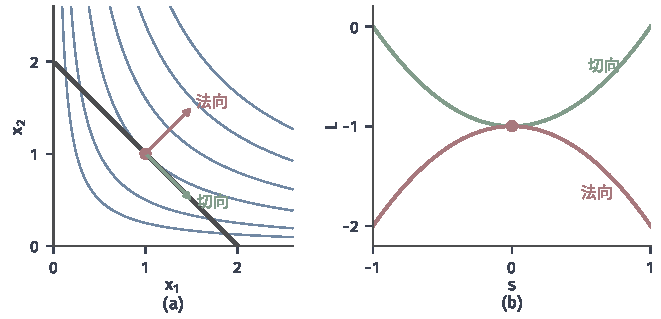
\includegraphics[width=112mm]{figures/05-optimization/06-constrained-optimization/matplotlib/sens-equality-tangent/figure.pdf}
 \caption{切空间上的正定性。(a)~蓝线是$x_1x_2$的等值线，深灰线是约束$x_1+x_2=2$，红点是解，绿色箭头是切方向，红色箭头是法方向。(b)~取$\nu=1$，Lagrange函数沿切方向$(1+s,1-s)$的值是$s^2-1$（绿线），沿法方向$(1+s,1+s)$的值是$-1-s^2$（红线）。}
 \label{fig:sens-equality-tangent}
\end{BookInlineFigure}

Lagrange函数对$\bm{x}$的梯度是
\[
 \nabla_{\bm{x}}\mathcal{L}=(-x_2+\nu\theta,\ -x_1+\nu),
\]
它对$\theta$的偏导数是$(\nu,0)$，而$\partial h/\partial\theta=x_1$。在基准点，这些量都已知，式~\eqref{eq:sens-equality-derivative}成为
\[
 \begin{bmatrix}0&-1&1\\-1&0&1\\1&1&0\end{bmatrix}
 \begin{bmatrix}x_1'\\x_2'\\\nu'\end{bmatrix}
 =-\begin{bmatrix}1\\0\\1\end{bmatrix}.
\]

第二行给出$\nu'=x_1'$，第一行给出$x_2'=x_1'+1$，代入第三行$x_1'+x_2'=-1$，得到
\[
 x_1'=-1,\qquad x_2'=0,\qquad\nu'=-1.
\]
这与显式解在$\theta=1$的导数一致：涨价时第一种投入减少，第二种投入不变。

如果把目标改成$+x_1x_2$，KKT矩阵仍然可逆，隐函数定理仍然给出同样的分支，但切方向的曲率变成$-2$，这条分支上全是约束极大点。可逆只说明方程的解光滑，极小性要靠曲率的符号。

\paragraph{去掉条件会怎样}
先去掉切空间正定性。考虑$\min\tfrac12x_2^2$，约束$x_2-\theta=0$。约束梯度$(0,1)$非零，但切方向$(1,0)$上$\bm{W}=\operatorname{diag}(0,1)$的曲率为零。此时$\bm{K}$的第一行全为零，矩阵奇异。解集是整条直线$\{(s,\theta):s\in\mathbb{R}\}$，“解的导数”没有确定的含义。

再去掉行满秩。考虑$\min x$，约束$x^2-\theta=0$。$\theta>0$时可行集是$\{\pm\sqrt{\theta}\}$，最小点是$x=-\sqrt{\theta}$，导数是$-1/(2\sqrt{\theta})$，$\theta\downarrow0$时趋于$-\infty$。在$\theta=0$处约束梯度$2x$为零，平稳条件$1+2x\nu=0$在$x=0$处没有解，KKT条件本身就不成立。

\subsection{不等式约束极小解}
\label{sec:sens-inequality}

不等式比等式多了一件事：哪些约束起作用，可能随参数改变。本小节的思路是，只要局部上活动约束不变，就把它们当作等式，回到上一小节的情形。

\paragraph{需要的三个条件}
考虑一般问题~\eqref{eq:sens-general-problem}，设$(\bm{x}_0,\bm{\lambda}_0,\bm{\nu}_0)$是$\bm{\theta}_0$处的KKT点，$A=\{i:g_i(\bm{x}_0,\bm{\theta}_0)=0\}$是活动集，$a$是其元素个数。这里用到第~\ref{chap:constrained-optimality}章的三个概念。

\begin{itemize}
 \item \emph{线性无关约束资格}（LICQ）：活动不等式的梯度和全部等式的梯度线性无关。
 \item \emph{严格互补}：每个活动不等式的乘子都严格为正，$\lambda_{0,i}>0$（$i\in A$）。
 \item \emph{二阶充分条件}：$\bm{W}=\nabla^2_{\bm{x}\bm{x}}\mathcal{L}$在临界锥上正定。严格互补成立时，临界锥就是子空间$\ker\bm{J}$，其中$\bm{J}$的行是活动不等式和全部等式的梯度。
\end{itemize}

把活动的不等式改写成等式，定义未知向量$\bm{w}=(\bm{\lambda}_A,\bm{\nu})$，得到一个缩减的方程组
\begin{equation}
 \bm{F}(\bm{x},\bm{w},\bm{\theta})=\begin{bmatrix}\nabla_{\bm{x}}\mathcal{L}\\\bm{g}_A(\bm{x},\bm{\theta})\\\bm{h}(\bm{x},\bm{\theta})\end{bmatrix}=\bm{0}.
 \label{eq:sens-reduced-kkt}
\end{equation}
活动约束的乘子和等式乘子是未知量，不活动约束的乘子取为零，不进入方程。

\begin{theorem}[不等式约束极小解的导数]
\label{thm:sens-inequality}
设$f,g_i,h_j$在$(\bm{x}_0,\bm{\theta}_0)$的邻域内二阶连续可微，$(\bm{x}_0,\bm{\lambda}_0,\bm{\nu}_0)$是KKT点，LICQ、严格互补与二阶充分条件成立。则存在$\bm{\theta}_0$的邻域和唯一的连续可微映射$(\bm{x}(\cdot),\bm{\lambda}(\cdot),\bm{\nu}(\cdot))$，它在基准处经过基准点，邻域内的每一点都是相应问题的KKT点，活动集恒为$A$，$\bm{x}(\bm{\theta})$是严格局部极小点。导数$\bm{D}_{\bm{x}}$、$\bm{D}_{\bm{w}}$满足
\begin{equation}
 \begin{bmatrix}\bm{W}&\bm{J}^{\top}\\\bm{J}&\bm{0}\end{bmatrix}
 \begin{bmatrix}\bm{D}_{\bm{x}}\\\bm{D}_{\bm{w}}\end{bmatrix}
 =-\begin{bmatrix}\nabla^2_{\bm{x}\bm{\theta}}\mathcal{L}\\\bm{D}_{\bm{\theta}}(\bm{g}_A,\bm{h})\end{bmatrix}.
 \label{eq:sens-inequality-derivative}
\end{equation}
\end{theorem}

\begin{proof}
LICQ就是$\bm{J}$行满秩，严格互补使二阶充分条件成为$\bm{W}$在$\ker\bm{J}$上正定。由引理~\ref{lem:sens-kkt-invertible}，矩阵$\bm{K}$可逆，隐函数定理给出式~\eqref{eq:sens-reduced-kkt}的连续可微解$(\bm{x}(\bm{\theta}),\bm{w}(\bm{\theta}))$，求导得到式~\eqref{eq:sens-inequality-derivative}。

下面验证这个解确实是完整问题的KKT点。不活动约束满足$g_i(\bm{x}_0,\bm{\theta}_0)<0$，由连续性，附近仍有$g_i(\bm{x}(\bm{\theta}),\bm{\theta})<0$，把它们的乘子取为零。活动约束的乘子满足$\lambda_{0,i}>0$，由连续性，附近仍有$\lambda_i(\bm{\theta})>0$。于是可行性、乘子符号和互补松弛全部成立，活动集仍是$A$，且严格互补仍成立。

与定理~\ref{thm:sens-equality}相同的连续性论证说明，$\bm{J}$行满秩和$\ker\bm{J}$上的正定性在附近保持，二阶充分条件推出$\bm{x}(\bm{\theta})$是严格局部极小点。

最后看唯一性。若完整问题另有KKT点靠近基准点，不活动约束仍严格满足，其乘子必为零；活动约束的乘子靠近正数$\lambda_{0,i}$，也为正，由互补松弛这些约束取等号。这个点于是满足式~\eqref{eq:sens-reduced-kkt}，由隐函数定理的唯一性，它就在分支上。
\end{proof}

图~\ref{fig:sens-kkt-block}画出式~\eqref{eq:sens-inequality-derivative}的结构。系数矩阵只由基准点的量决定，$q$个参数对应$q$列右端。

\begin{BookInlineFigure}
 \centering
 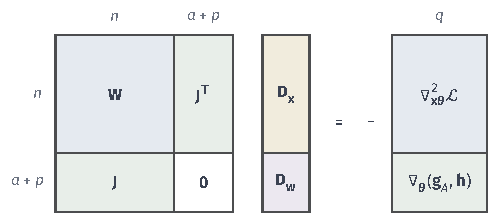
\includegraphics[width=83mm]{figures/05-optimization/06-constrained-optimization/tikz/sens-kkt-block/figure.pdf}
 \caption{式~\eqref{eq:sens-inequality-derivative}的分块结构。系数矩阵的阶数是$n+a+p$，其中$a$是活动不等式个数，$p$是等式个数。$\bm{D}_{\bm{x}}$与$\bm{D}_{\bm{w}}$是待求的Jacobian矩阵，右端共$q$列，每列对应一个参数。不活动约束不出现在这个方程组中。}
 \label{fig:sens-kkt-block}
\end{BookInlineFigure}

\paragraph{预算例的两个活动集}
取$\tau=2$。活动集是$\{1\}$，方程组与第~\ref{sec:sens-equality}节的预算线例子完全相同，因为只有预算在起作用：
\[
 x_1'=x_2'=\frac12,\qquad\lambda_1'=-\frac12.
\]

取$\tau=0.5$。解是$(0.5,0)$，乘子是$\lambda_1=3/2$，$\lambda_3=1/2$，活动集是$\{1,3\}$。此时$\bm{W}=\bm{I}$，活动约束的梯度组成
\[
 \bm{J}=\begin{bmatrix}1&1\\0&-1\end{bmatrix},\qquad
 \frac{\partial}{\partial\tau}\begin{bmatrix}g_1\\g_3\end{bmatrix}=\begin{bmatrix}-1\\0\end{bmatrix}.
\]

$\ker\bm{J}$只含零向量，切空间的正定性自动成立。式~\eqref{eq:sens-inequality-derivative}的四行分别是
\[
 x_1'+\lambda_1'=0,\quad
 x_2'+\lambda_1'-\lambda_3'=0,\quad
 x_1'+x_2'=1,\quad
 -x_2'=0.
\]
依次解出
\[
 x_2'=0,\qquad x_1'=1,\qquad\lambda_1'=-1,\qquad\lambda_3'=-1.
\]
这时增加的预算全部给第一种投入，因为$x_2$被边界挡在零上。

\paragraph{严格互补和余量给出窗口}
严格互补与不活动约束的严格余量在定理中起同一种作用：它们留出一段余地，让参数小幅变化时符号条件不被破坏。这段余地有多大，可以用导数估计。

在$\tau=2$处，三个要保持为正的量分别是不活动约束的余量$x_1$、$x_2$和活动约束的乘子$\lambda_1$。沿分支它们是
\[
 x_1=\frac{\tau+1}{2},\qquad
 x_2=\frac{\tau-1}{2},\qquad
 \lambda_1=\frac{3-\tau}{2}.
\]

第一个到达零的是$x_2$（$\tau=1$）和$\lambda_1$（$\tau=3$），分支的有效窗口是$1<\tau<3$，见图~\ref{fig:sens-margins}。窗口的一端是不活动约束变成活动，另一端是活动约束不再起作用。

\begin{BookInlineFigure}
 \centering
 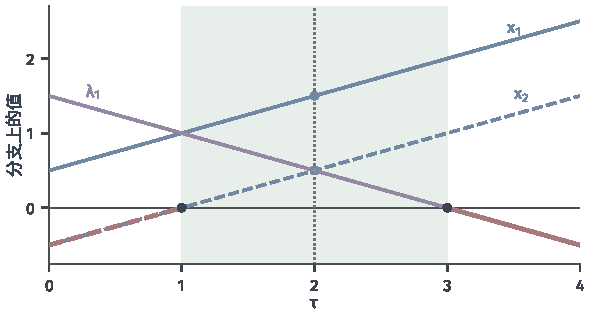
\includegraphics[width=100mm]{figures/05-optimization/06-constrained-optimization/matplotlib/sens-margins/figure.pdf}
 \caption{活动集$\{1\}$的分支把公式延拓到窗口之外。蓝色实线与虚线是不活动约束的余量$x_1$、$x_2$，紫线是乘子$\lambda_1$，绿色区域是三者都为正的窗口$1<\tau<3$。红色部分是符号条件被破坏之处：$\tau<1$时$x_2<0$不可行，$\tau>3$时$\lambda_1<0$不满足KKT条件。}
 \label{fig:sens-margins}
\end{BookInlineFigure}

\paragraph{这些条件只是充分的}
定理的三个条件对解可微是充分条件，下面三个例子逐一说明它们都不是必要的。

严格互补不必要：考虑$\min\tfrac12(x-\theta^2)^2$，约束$x\geq0$。解是$x=\theta^2$，处处可微。而在$\theta=0$处，约束活动且乘子为零，严格互补不成立。

LICQ不必要：约束写两遍$\theta-x\leq0$，目标取$\min x$。解$x=\theta$处处可微，两条活动约束的梯度相同，LICQ不成立，乘子也不唯一。

二阶充分条件不必要：考虑$\min x^4/4-\theta^3x$，驻点方程$x^3=\theta^3$给出$x=\theta$，处处可微。而在$\theta=0$处Hessian等于零。

反过来，这些条件被破坏时，导数常常确实失效，下一节拆开具体的失效方式。定理不能用来断言“条件不成立，所以不可微”。

\section{分支变化}
\label{sec:sens-branches}

上一节的局部导数有前提。前提不成立时，导数为什么会失效，失效的方式有什么不同？本节用三个能够手算的例子回答。活动集改变时，可用的方程变了。全局最优解切换时，所选的分支变了。方程退化时，线性方程不再可逆。三种情况的数学原因不同，都不是某个算法的不稳定。

\subsection{活动集改变}
\label{sec:sens-active-change}

\paragraph{分段解出预算例}
把预算例按活动集分成三段，每段都用KKT条件解出。

当$\tau>3$时，理想点$(2,1)$满足$x_1+x_2\leq\tau$，全部约束不起作用：
\[
 \bm{x}^\star=(2,1),\qquad\bm{\lambda}=\bm{0},\qquad V(\tau)=0.
\]

当$1<\tau<3$时，只有预算起作用。平稳条件是$x_1-2+\lambda_1=0$、$x_2-1+\lambda_1=0$，代入$x_1+x_2=\tau$，得到$3-2\lambda_1=\tau$，于是
\[
 \lambda_1=\frac{3-\tau}{2},\qquad
 \bm{x}^\star=\Bigl(\frac{\tau+1}{2},\ \frac{\tau-1}{2}\Bigr).
\]
两个坐标与乘子在这段都是正的。目标值是$\lambda_1^2$，即$V(\tau)=(3-\tau)^2/4$。

当$0<\tau<1$时，预算和$x_2\geq0$起作用，$\bm{x}^\star=(\tau,0)$。平稳条件的两个分量是$x_1-2+\lambda_1=0$和$x_2-1+\lambda_1-\lambda_3=0$，由此解出
\[
 \lambda_1=2-\tau,\qquad\lambda_3=1-\tau.
\]
两者都为正。目标值是
\[
 V(\tau)=\frac12(2-\tau)^2+\frac12.
\]

\begin{BookInlineTable}
 \centering
 \begin{tabular}{cccc}
  \toprule
  区间 & $\bm{x}^\star(\tau)$ & $(\lambda_1,\lambda_3)$ & $V'(\tau)$\\
  \midrule
  $0<\tau<1$ & $(\tau,\ 0)$ & $(2-\tau,\ 1-\tau)$ & $\tau-2$\\
  $1<\tau<3$ & $\bigl(\frac{\tau+1}{2},\ \frac{\tau-1}{2}\bigr)$ & $\bigl(\frac{3-\tau}{2},\ 0\bigr)$ & $\frac{\tau-3}{2}$\\
  $\tau>3$ & $(2,\ 1)$ & $(0,\ 0)$ & $0$\\
  \bottomrule
 \end{tabular}
 \caption{预算例的三段解，$\lambda_2$在所有区间都等于零。每一段内$V'(\tau)=-\lambda_1$，这正是乘子的边际解释。}
 \label{tab:sens-budget-pieces}
\end{BookInlineTable}

\paragraph{连接点上发生了什么}
图~\ref{fig:sens-activeset-path}画出解在平面上的路径，图~\ref{fig:sens-activeset-curves}画出各个量随$\tau$的变化。解的路径是一条折线，在$\tau=1$与$\tau=3$处转弯。

\begin{BookInlineFigure}
 \centering
 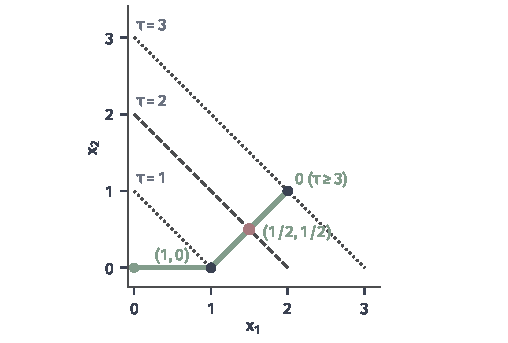
\includegraphics[width=86mm]{figures/05-optimization/06-constrained-optimization/matplotlib/sens-activeset-path/figure.pdf}
 \caption{最优解$\bm{x}^\star(\tau)$在平面上的路径（绿线）。虚线与点线是几条预算线，黑点是活动集改变的位置，红点是$\tau=2$的解。绿色文字是各段上解对$\tau$的导数：第一段$(1,0)$，第二段$(1/2,1/2)$，$\tau\geq3$时为零。}
 \label{fig:sens-activeset-path}
\end{BookInlineFigure}

$\tau=1$处，$x_2\geq0$刚要失去作用，$\lambda_3=0$。$\tau=3$处，预算刚要失去作用，$\lambda_1=0$。两处都有活动约束的乘子等于零，严格互补恰好在连接点失败。

解在连接点连续但不可微。$\tau=1$处的左导数和右导数分别是
\[
 \bm{x}'(1^-)=(1,0),\qquad\bm{x}'(1^+)=\Bigl(\frac12,\frac12\Bigr).
\]
值函数却不一样。两段的$V'$在$\tau=1$处都等于$-1$，在$\tau=3$处都等于$0$，所以$V$在连接点可微，只是二阶导数有跳跃。原因是$V'=-\lambda_1$，而$\lambda_1$连续穿过连接点：进入或离开活动集的约束，它的乘子在那里恰好是零，不造成$\lambda_1$的跳变。

\begin{BookInlineFigure}
 \centering
 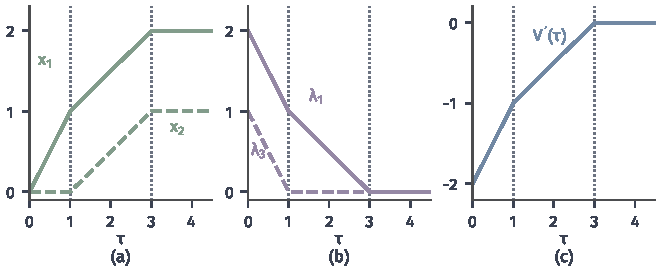
\includegraphics[width=112mm]{figures/05-optimization/06-constrained-optimization/matplotlib/sens-activeset-curves/figure.pdf}
 \caption{预算例各量随$\tau$的变化，灰色点线标出$\tau=1,3$。(a)~解的两个分量（实线$x_1$，虚线$x_2$）在连接点转折。(b)~乘子$\lambda_1$（实线）、$\lambda_3$（虚线）连续，但斜率改变。(c)~$V'(\tau)$连续，说明$V$在连接点仍然可微。}
 \label{fig:sens-activeset-curves}
\end{BookInlineFigure}

\paragraph{固定活动集的公式不能外推}
公式必须限定在它的区间内使用。把活动集$\{1\}$的公式用到$\tau=0.5$，得到$x_2=-0.25$，不可行。用到$\tau=4$，得到$\lambda_1=-1/2$，乘子符号错误。这两种错误恰好给出判别方法：预测的不活动约束是否越界，预测的乘子是否变负。

连接点上只有单侧的导数。向哪一侧走，就要换用那一侧的活动集重新写方程，上面的$\bm{x}'(1^-)$和$\bm{x}'(1^+)$正是这样得到的。

\subsection{全局最优解切换}
\label{sec:sens-global-switch}

\paragraph{两个候选的比较}
活动集改变时解连续地走过连接点。全局最优解还可能在两个相距很远的候选之间跳动。最简单的例子是在两点集合上选最小：
\begin{equation}
 \min_{x\in\{-1,1\}}\ \theta x.
 \label{eq:sens-two-points}
\end{equation}
把两个候选分别看成两条分支：
\[
 x=1:\quad v_1(\theta)=\theta,\qquad\qquad
 x=-1:\quad v_2(\theta)=-\theta.
\]
每条分支上解都是常数，$\bm{x}'=0$，值是线性函数，两者都光滑。

全局最优值取两条分支的较小者，最优解集合随$\theta$的符号改变：
\begin{equation}
 V(\theta)=-\lvert\theta\rvert,\qquad
 \bm{S}(\theta)=\begin{cases}\{1\},&\theta<0,\\\{-1,1\},&\theta=0,\\\{-1\},&\theta>0.\end{cases}
 \label{eq:sens-switching}
\end{equation}

图~\ref{fig:sens-switching}分别显示了三件事。每条分支在$\theta=0$处都很光滑。全局值在$\theta=0$处不可微。解集合在$\theta=0$处从一个点变成两个点，再变回另一个点，选出的解不连续。

\begin{BookInlineFigure}
 \centering
 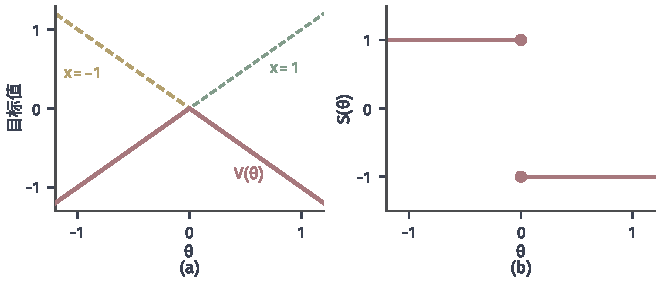
\includegraphics[width=112mm]{figures/05-optimization/06-constrained-optimization/matplotlib/sens-switching/figure.pdf}
 \caption{在$\{-1,1\}$上最小化$\theta x$。(a)~绿色虚线是$x=1$分支的值，黄色虚线是$x=-1$分支的值，红线是全局最优值$-\lvert\theta\rvert$。(b)~全局最优解集合，$\theta=0$处两个点都最优，解在此跳跃。}
 \label{fig:sens-switching}
\end{BookInlineFigure}

\paragraph{三个对象分别的结论}
定理~\ref{thm:sens-danskin}在这里成立：$\bm{C}=\{-1,1\}$是紧集，$\partial f/\partial\theta=x$连续。在$\theta=0$处，它给出
\[
 V'(0;d)=\min_{x\in\{-1,1\}}xd=-\lvert d\rvert,
\]
这与$V(\theta)=-\lvert\theta\rvert$一致。

把一条分支的导数推广成全局公式是常见的错误。$x=1$分支的导数在$\theta>0$时仍然是$1$，但$\theta>0$时全局最优解已经是$-1$，全局值的导数是$-1$。第~\ref{sec:sens-problems}节的双谷目标在连续变量上重现了同样的现象：每个谷底都有光滑的分支，全局最优解在$\theta=0$处跳到另一个谷底。在双谷的右侧分支上，驻点方程$4x^3-4x+\theta=0$对$x$的导数在$x=1$处是$8$，隐函数定理给出
\[
 x'(0)=-\frac{1}{8}.
\]
这个导数描述的是右侧谷底的移动，与全局最优解在$\theta=0$处的跳跃无关。

\subsection{退化与变化尺度}
\label{sec:sens-degeneracy}

前两种失效换了方程或换了分支。第三种失效中方程和分支都没有换，解甚至唯一，只是线性化之后的方程退化了。

\paragraph{唯一解也可能没有有限导数}
考虑
\begin{equation}
 \min_{x\in\mathbb{R}}\ \frac14x^4-\theta x.
 \label{eq:sens-quartic}
\end{equation}
对每个$\theta$，目标严格凸且强制，最优解唯一。驻点方程$x^3=\theta$给出
\[
 x^\star(\theta)=\theta^{1/3}.
\]

$\theta=0$处$x^\star=0$，Hessian$3x^2$等于零，隐函数定理的条件不成立。真实导数是
\[
 \frac{\mathrm{d}x^\star}{\mathrm{d}\theta}=\frac{1}{3\theta^{2/3}}\quad(\theta\neq0),
\]
$\theta\to0$时趋于$+\infty$，解函数在$\theta=0$处有竖直的切线。参数变化$10^{-6}$，解移动$10^{-2}$，一万倍的放大，见图~\ref{fig:sens-quartic}(b)。

值函数却没有这个问题。把解代入，
\[
 V(\theta)=\frac14\theta^{4/3}-\theta^{4/3}=-\frac34\lvert\theta\rvert^{4/3},
\]
并且$V'(\theta)=-\theta^{1/3}$，在$\theta=0$处等于零。这正是包络关系：$\partial f/\partial\theta=-x$，只需知道解的位置，不需要它的导数。再一次看到，值比解更稳定。

\begin{BookInlineFigure}
 \centering
 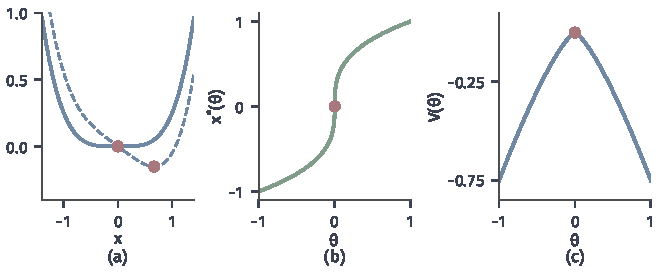
\includegraphics[width=112mm]{figures/05-optimization/06-constrained-optimization/matplotlib/sens-quartic/figure.pdf}
 \caption{退化的唯一最优解。(a)~目标$x^4/4-\theta x$，实线$\theta=0$，虚线$\theta=0.3$，红点是最小点。$\theta=0$时谷底二阶平坦。(b)~最优解$\theta^{1/3}$在$\theta=0$处切线竖直。(c)~最优值$-\tfrac34\lvert\theta\rvert^{4/3}$在$\theta=0$处可微。}
 \label{fig:sens-quartic}
\end{BookInlineFigure}

\paragraph{非退化时的放大倍数}
矩阵$\bm{K}$可逆但接近奇异时，导数存在却很大。记$\bm{z}=(\bm{x},\bm{w})$，$\bm{B}=\bm{D}_{\bm{\theta}}\bm{F}$。由式~\eqref{eq:sens-inequality-derivative}，一阶变化满足$\bm{K}\Delta\bm{z}=-\bm{B}\Delta\bm{\theta}$，因此
\begin{equation}
 \lVert\Delta\bm{z}\rVert_2\leq\lVert\bm{K}^{-1}\rVert_2\,\lVert\bm{B}\Delta\bm{\theta}\rVert_2.
 \label{eq:sens-amplification}
\end{equation}
$\lVert\bm{K}^{-1}\rVert_2$越大，同样的参数变化引起的解和乘子的变化可能越大。下面两种几何情形都会使它变大。

第一种是约束接近平行。取两条等式约束
\[
 x_1+x_2=\tau,\qquad x_1+(1+\varepsilon)x_2=2+\varepsilon.
\]
解由它们的交点确定，$\tau=2$时交点是$(1,1)$。解线性方程，得到
\[
 \bm{x}'(\tau)=\Bigl(\frac{1+\varepsilon}{\varepsilon},\ -\frac{1}{\varepsilon}\Bigr).
\]

$\varepsilon=0.25$时导数是$(5,-4)$，$\varepsilon=0.01$时是$(101,-100)$。约束梯度仍然线性无关，LICQ成立，只是接近失效。图~\ref{fig:sens-amplification}(a)里，预算线只平移一点，交点却沿着两条线滑过很长的距离。

第二种是碗的底部很平。考虑二次目标
\[
 f(\bm{x},\bm{b})=\frac12\bm{x}^{\top}\bm{H}\bm{x}-\bm{b}^{\top}\bm{x},\qquad\bm{H}=\operatorname{diag}(1,0.1).
\]
把$b_2$从$0.1$改为$0.2$，解从$(1,1)$移到$(1,2)$。参数只变化$0.1$，解移动了$1$，放大倍数是曲率的倒数，即$10$。

\begin{BookInlineFigure}
 \centering
 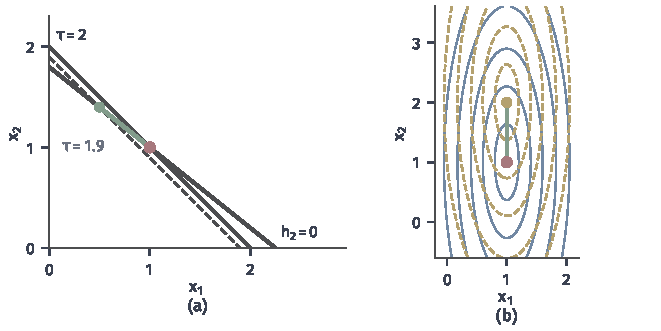
\includegraphics[width=112mm]{figures/05-optimization/06-constrained-optimization/matplotlib/sens-amplification/figure.pdf}
 \caption{两种放大机制。(a)~$\varepsilon=0.25$的两条等式约束，预算线从实线$\tau=2$平移到虚线$\tau=1.9$，交点沿绿色线段从红点移到绿点，距离约是平移量的$6.4$倍。(b)~$\bm{H}=\operatorname{diag}(1,0.1)$的目标等高线，蓝色实线是$b_2=0.1$，黄色虚线是$b_2=0.2$，最小点沿绿色线段从红点移到黄点。}
 \label{fig:sens-amplification}
\end{BookInlineFigure}

\paragraph{固有敏感性与数值误差}
上面的放大是问题的性质，与用什么算法无关。这里有两种不同的误差，需要分开。

\begin{BookInlineTable}
 \centering
 \begin{tabular}{lll}
  \toprule
  & 固有敏感性 & 数值误差\\
  \midrule
  比较 & 不同参数的精确解 & 同一问题的计算解与精确解\\
  度量 & $\bm{D}\bm{z}$的大小 & 残差、舍入与条件数\\
  改善 & 改变模型或数据 & 改进算法与精度\\
  \bottomrule
 \end{tabular}
 \caption{固有敏感性与数值误差的比较。两者都可能与$\bm{K}$的病态有关，但回答不同的问题。}
 \label{tab:sens-inherent-numerical}
\end{BookInlineTable}

矩阵的条件数大，并不一定说明解对参数敏感。把预算例中预算约束整体乘以$s>0$，写成$s(x_1+x_2-\tau)\leq0$。这是同一个约束，解不变，解对$\tau$的导数也不变，乘子则变成原来的$1/s$。相应的KKT矩阵是
\[
 \bm{K}_s=\begin{bmatrix}1&0&s\\0&1&s\\s&s&0\end{bmatrix}.
\]
$s=1$时条件数是$2$。$s=1000$时条件数约为$1415$，而$\bm{x}'(\tau)$仍然是$(1/2,1/2)$。这里的条件数变大只反映约束的书写尺度，解的敏感性没有任何变化。

解读式~\eqref{eq:sens-amplification}之前，应该先把变量和约束调整到量纲合理的尺度，计算时也应该作相应的平衡处理。只有这样，$\bm{K}$的病态才能反映问题真实的敏感性。

\section{导数的计算与核验}
\label{sec:sens-computation}

局部导数的公式已经有了，怎样计算它们，又怎样确认算出的结果可信？

\paragraph{主要思想：一次分解，多个右端}
式~\eqref{eq:sens-inequality-derivative}的系数矩阵$\bm{K}$只依赖基准点，右端$\bm{B}$的每一列对应一个参数。记$N=n+a+p$，把待求的两块Jacobian矩阵合写成
\[
 \bm{Z}=\begin{bmatrix}\bm{D}_{\bm{x}}\\\bm{D}_{\bm{w}}\end{bmatrix}\in\mathbb{R}^{N\times q}.
\]
需要解的是
\begin{equation}
 \bm{K}\bm{Z}=-\bm{B}.
 \label{eq:sens-compute}
\end{equation}
这相当于同一个矩阵配上$q$个右端，只需分解一次，然后对每一列回代。不需要对每个参数重解一次原来的非线性问题。$\bm{K}$对称而不定，通常用带主元选取的$\bm{L}\bm{D}\bm{L}^{\top}$分解，分解的做法可参考\BookChapterRef{chap:direct-linear-solvers}{卷二第12章“线性方程的直接求解”}。

分解还可以顺便检查极小性。$\bm{J}$行满秩时，$\bm{W}$在$\ker\bm{J}$上正定，当且仅当$\bm{K}$恰有$n$个正特征值、$a+p$个负特征值、没有零特征值。这称为\term{惯性}（inertia）判别，证明可查阅\scite{math-nocedal2006numerical}。$\bm{L}\bm{D}\bm{L}^{\top}$分解的$\bm{D}$与$\bm{K}$合同，读出$\bm{D}$的正负特征值个数，就得到惯性，不必另算。

\paragraph{主要思想：只要一个输出时用伴随}
有时我们并不需要整个$\bm{D}_{\bm{x}}$，只要一个标量输出$\phi(\bm{x}(\bm{\theta}))$对$q$个参数的梯度。这时梯度是
\[
 \nabla_{\bm{\theta}}\phi=\bm{D}_{\bm{x}}^{\top}\bm{c},\qquad\bm{c}=\nabla\phi(\bm{x}).
\]
代入式~\eqref{eq:sens-compute}，并在$\bm{c}$后面补零以匹配维数，就是
\begin{equation}
 \nabla_{\bm{\theta}}\phi=-\bm{B}^{\top}\bm{r},\qquad
 \bm{K}\bm{r}=\begin{bmatrix}\bm{c}\\\bm{0}\end{bmatrix}.
 \label{eq:sens-adjoint}
\end{equation}

这里用到$\bm{K}$对称。式~\eqref{eq:sens-adjoint}只解一个线性方程，与参数个数无关。这种做法称为\term{伴随法}（adjoint method）。两种算法的差别只是矩阵乘积$\bm{c}^{\top}\bm{K}^{-1}\bm{B}$的结合顺序不同，见图~\ref{fig:sens-forward-adjoint}。

\begin{BookInlineFigure}
 \centering
 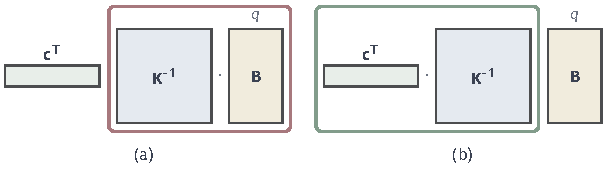
\includegraphics[width=103mm]{figures/05-optimization/06-constrained-optimization/tikz/sens-forward-adjoint/figure.pdf}
 \caption{同一乘积$\bm{c}^{\top}\bm{K}^{-1}\bm{B}$的两种结合顺序。(a)~先算红框内的$\bm{K}^{-1}\bm{B}$，每个参数一个右端，得到全部的$\bm{D}_{\bm{x}}$。(b)~先算绿框内的$\bm{c}^{\top}\bm{K}^{-1}$，只有一个右端，得到单个输出对全部参数的梯度。}
 \label{fig:sens-forward-adjoint}
\end{BookInlineFigure}

表~\ref{tab:sens-cost}比较各种做法的成本，规模变量为$N$与$q$，运算量只计首项。重新求解一列的成本指做一次完整的$\bm{K}$分解，实际的非线性重解通常更贵。$\bm{K}$稀疏时，分解成本由消元产生的填充决定，回代成本是$\bm{L}$的非零元个数的两倍，表中的立方、平方相应缩小，分解一次多次回代的比例关系不变。

\begin{BookInlineTable}
 \centering
 \begin{tabular}{lll}
  \toprule
  做法 & 稠密运算量 & 得到什么\\
  \midrule
  每个参数重解 & $qN^3/3$ & 全部$\bm{D}_{\bm{x}}$\\
  一次分解，$q$次回代 & $N^3/3+2qN^2$ & 全部$\bm{D}_{\bm{x}}$和$\bm{D}_{\bm{w}}$\\
  伴随法 & $N^3/3+2N^2$ & 一个输出的梯度\\
  \bottomrule
 \end{tabular}
 \caption{计算解对参数导数的稠密运算量，$N=n+a+p$。分解的复用要求活动集不变。伴随法的结果再乘$\bm{B}^{\top}$需要的运算量与$\bm{B}$的非零元个数成正比。}
 \label{tab:sens-cost}
\end{BookInlineTable}

\paragraph{计算过程}
下面把全过程用在一个小例子上。预算例中同时考虑两个参数，预算$\tau$和理想点的横坐标偏移$\theta$，基准是$(\tau,\theta)=(2,0)$，目标是
\[
 f(\bm{x},\theta)=\frac12(x_1-2-\theta)^2+\frac12(x_2-1)^2.
\]

\needspace{6\baselineskip}
\paragraph{变量}
\begin{itemize}
 \item 基准解$\bm{x}\in\mathbb{R}^n$，活动乘子与等式乘子合写成$\bm{w}\in\mathbb{R}^{a+p}$。
 \item 系数矩阵$\bm{K}\in\mathbb{R}^{N\times N}$，右端$\bm{B}\in\mathbb{R}^{N\times q}$，$N=n+a+p$。
 \item 输出$\bm{Z}$，形状是$N\times q$，含$\bm{D}_{\bm{x}}$与$\bm{D}_{\bm{w}}$两块。
 \item 每个不活动约束的余量，每个活动约束的乘子，它们决定分支的有效范围。
\end{itemize}

\paragraph{初始化}
先把基准问题求解到足够高的精度，读出解和乘子，再分出活动约束。

例中$n=2$，$a=1$，$p=0$，$q=2$。基准解和乘子是
\[
 \bm{x}=\begin{bmatrix}3/2\\1/2\end{bmatrix},\qquad\lambda_1=\frac12,\qquad A=\{1\}.
\]

\paragraph{计算步骤}
\begin{enumerate}
 \item 组装$\bm{K}$和$\bm{B}$，公式见式~\eqref{eq:sens-inequality-derivative}。

 例中Lagrange函数的梯度和活动约束分别是
 \[
  \nabla_{\bm{x}}\mathcal{L}=(x_1-2-\theta+\lambda_1,\ x_2-1+\lambda_1),\quad g_1=x_1+x_2-\tau,
 \]
 对$\bm{x}$、$\lambda_1$和$(\tau,\theta)$分别求偏导，得到
 \[
  \bm{K}=\begin{bmatrix}1&0&1\\0&1&1\\1&1&0\end{bmatrix},\qquad
  \bm{B}=\begin{bmatrix}0&-1\\0&0\\-1&0\end{bmatrix}.
 \]
 $\bm{B}$的第一列对应$\tau$，第二列对应$\theta$。

 \item 分解$\bm{K}=\bm{L}\bm{D}\bm{L}^{\top}$，并由$\bm{D}$的符号检查惯性。

 例中不需要主元交换，消元得到
 \[
  \bm{L}=\begin{bmatrix}1&0&0\\0&1&0\\1&1&1\end{bmatrix},\qquad
  \bm{D}=\operatorname{diag}(1,1,-2).
 \]
 $\bm{D}$有两个正数和一个负数，与$n=2$，$a=1$相符，这个解是局部极小点。

 \item 对$\bm{B}$的每一列回代，得到$\bm{Z}$的相应列，公式见式~\eqref{eq:sens-compute}。

 例中$\tau$列的右端是$(0,0,1)^{\top}$。依次解$\bm{L}\bm{y}=(0,0,1)^{\top}$、$\bm{D}\bm{y}'=\bm{y}$、$\bm{L}^{\top}\bm{z}=\bm{y}'$，中间结果和最终结果是
 \[
  \bm{y}=\begin{bmatrix}0\\0\\1\end{bmatrix},\quad
  \bm{y}'=\begin{bmatrix}0\\0\\-1/2\end{bmatrix},\quad
  \bm{z}=\begin{bmatrix}1/2\\1/2\\-1/2\end{bmatrix}.
 \]

 $\theta$列的右端是$(1,0,0)^{\top}$，同样回代，得到
 \[
  \bm{y}=\begin{bmatrix}1\\0\\-1\end{bmatrix},\quad
  \bm{y}'=\begin{bmatrix}1\\0\\1/2\end{bmatrix},\quad
  \bm{z}=\begin{bmatrix}1/2\\-1/2\\1/2\end{bmatrix}.
 \]

 \item 用余量和乘子确定有效范围。把导数代入，对方向$(\Delta\tau,\Delta\theta)$写出需要保持为正的量。

 例中这三个量分别是
 \[
  \begin{aligned}
  \lambda_1&=\frac12-\frac12\Delta\tau+\frac12\Delta\theta,\\
  x_1&=\frac32+\frac12\Delta\tau+\frac12\Delta\theta,\\
  x_2&=\frac12+\frac12\Delta\tau-\frac12\Delta\theta.
  \end{aligned}
 \]
 它们都大于零的区域是参数平面上的一个多面体，图~\ref{fig:sens-critical-regions}中绿色的带形就是这个区域在图中范围内的部分。

 \item 给出预测，并用小幅参数重求解核验：预测的活动集是否保持，预测的解与重解的结果相差多少。

 例中取$(\Delta\tau,\Delta\theta)=(0.2,0.1)$，三个量都为正，预测和重解都是
 \[
  \bm{x}=(1.65,\ 0.55),\qquad\lambda_1=0.45.
 \]
 问题在这个活动集上是二次的，所以预测是精确的。若取$(\Delta\tau,\Delta\theta)=(-1.5,0)$，预测给出$x_2=-1/4<0$，这说明活动集已经改变，需要换到活动集$\{1,3\}$重新计算，真实解是$(0.5,0)$。
\end{enumerate}

整个计算是一次完成的，没有迭代，到步骤五结束。最终得到
\[
 \bm{D}_{\bm{x}}=\begin{bmatrix}1/2&1/2\\1/2&-1/2\end{bmatrix},\qquad
 \bm{D}_{\lambda_1}=\begin{bmatrix}-1/2&1/2\end{bmatrix}.
\]

\begin{BookInlineFigure}
 \centering
 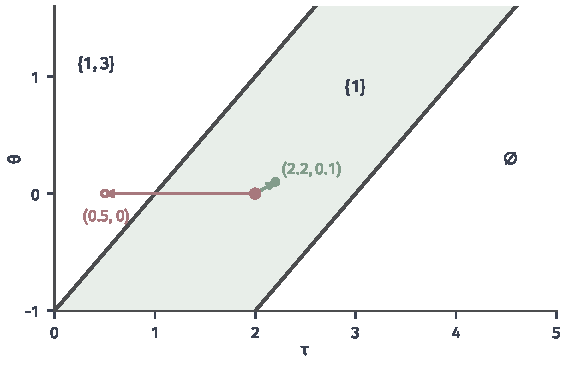
\includegraphics[width=96mm]{figures/05-optimization/06-constrained-optimization/matplotlib/sens-critical-regions/figure.pdf}
 \caption{参数平面$(\tau,\theta)$上的活动集区域。两条深灰线是$\tau=1+\theta$和$\tau=3+\theta$，它们划分出活动集$\{1,3\}$、$\{1\}$和$\varnothing$。红点是基准$(2,0)$，绿色箭头走到同一区域内的$(2.2,0.1)$，一阶预测有效；红色箭头越过边界到$(0.5,0)$，一阶预测失效。}
 \label{fig:sens-critical-regions}
\end{BookInlineFigure}

伴随法在这个例子上也可以手算。设只关心输出$\phi=x_2$，$\bm{c}=(0,1)^{\top}$。由式~\eqref{eq:sens-adjoint}，解$\bm{K}\bm{r}=(0,1,0)^{\top}$，得到$\bm{r}=(-1/2,1/2,1/2)^{\top}$，再求
\[
 \nabla_{(\tau,\theta)}x_2=-\bm{B}^{\top}\bm{r}=\begin{bmatrix}1/2\\-1/2\end{bmatrix}.
\]
这正是$\bm{D}_{\bm{x}}$的第二行，一次回代就得到了两个参数的结果。

\paragraph{算法分析：误差的三个来源}
隐式导数的公式对应精确的最优性方程。实际算出的导数还带有三种误差，它们的性质不同。

第一种是近似解带来的误差。基准解只解到$\tilde{\bm{x}}$，$\bm{K}$和$\bm{B}$都在$\tilde{\bm{x}}$处组装，导数的误差与解的误差成正比，比例系数由$\bm{K}^{-1}$和二阶导数的变化率决定。参数只出现在线性项时$\bm{B}$不依赖于$\bm{x}$，二次目标下这项误差为零。

第二种是有限差分的误差。用重解来核验导数时，常用中心差分
\[
 \frac{\bm{x}(\bm{\theta}+h\bm{d})-\bm{x}(\bm{\theta}-h\bm{d})}{2h},
\]
截断误差是$O(h^2)$。若每次重解的误差是$\varepsilon$，差分会放大成$O(\varepsilon/h)$。两项相加的误差在$h\sim\varepsilon^{1/3}$时最小，约为$\varepsilon^{2/3}$。

第三种是算法展开的误差。把迭代算法写成关于$\bm{\theta}$的函数，对$T$步迭代逐步求导，得到的是$\bm{x}^{(T)}$的导数，而不是$\bm{x}^\star$的导数。以梯度下降为例，它的迭代是
\[
 \bm{x}^{(t+1)}=\bm{x}^{(t)}-\alpha\nabla_{\bm{x}}f(\bm{x}^{(t)},\bm{\theta}),
\]
导数的递推式是
\begin{equation}
 \bm{D}^{(t+1)}=\bigl(\bm{I}-\alpha\nabla^2_{\bm{x}\bm{x}}f\bigr)\bm{D}^{(t)}-\alpha\nabla^2_{\bm{x}\bm{\theta}}f,
 \label{eq:sens-unroll}
\end{equation}
其中各导数都在$(\bm{x}^{(t)},\bm{\theta})$处取值。它的不动点正是式~\eqref{eq:sens-unconstrained-derivative}。

图~\ref{fig:sens-fd-unroll}用具体计算展示了这些误差。(a)中，差分误差先随$h$减小而减小，到某个$h$之后反而增大，这个转折点随求解精度$\varepsilon$移动。(b)在岭回归例子上比较了式~\eqref{eq:sens-unroll}的展开和在当前迭代点上计算的隐式导数：$\gamma$改变了曲率，展开的误差多了一个随$t$增长的因子，所以比隐式导数略慢。

\begin{BookInlineFigure}
 \centering
 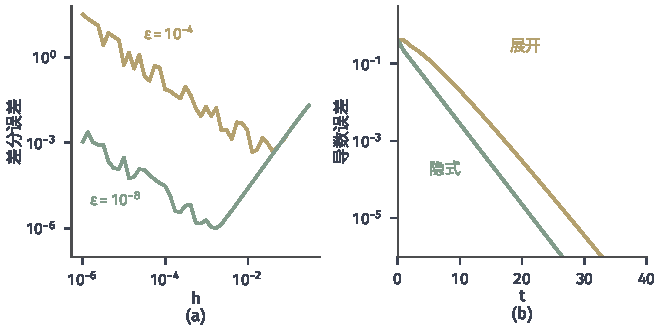
\includegraphics[width=112mm]{figures/05-optimization/06-constrained-optimization/matplotlib/sens-fd-unroll/figure.pdf}
 \caption{导数计算的误差。(a)~价格例$\theta=1$处$x_2$对$\theta$的中心差分误差。每次重解用梯度下降到残差$\varepsilon$，曲线取$40$次随机起点的中位数，黄线$\varepsilon=10^{-4}$，绿线$\varepsilon=10^{-8}$。(b)~岭回归例$\gamma=1$，步长$\alpha=1/L$，黄线是展开$t$步梯度下降得到的导数的误差，绿线是在$\bm{x}^{(t)}$处计算隐式导数的误差。}
 \label{fig:sens-fd-unroll}
\end{BookInlineFigure}

\paragraph{算法分析：非二次问题的核验}
第~\ref{sec:sens-general-constraints}节的价格例不是二次的，一阶预测有误差，可以检验误差的阶。在$\theta=1$处，由$\lambda'(1)=1$，$x_1'=1-\lambda-\lambda'\theta=-1/2$，$x_2'=-\lambda'=-1$。与重解的结果比较，
\[
 \begin{aligned}
 h&=0.1:\quad \bm{x}=(1.4480,\ 0.4072),\quad\text{预测}\ (1.45,\ 0.4),\\
 h&=0.01:\quad \bm{x}=(1.49498,\ 0.49007),\quad\text{预测}\ (1.495,\ 0.49).
 \end{aligned}
\]
误差分别约为$7.5\times10^{-3}$和$7.9\times10^{-5}$，$h$缩小十倍，误差缩小约一百倍，与二阶截断误差一致。

这个一致性只在活动集保持时成立。价格例的预算活动窗口是$(\sqrt{5}-1)/2<\theta<2$，$\theta>2$时$x_2\geq0$起作用。图~\ref{fig:sens-prediction-error}(b)中，$h$接近$1$时误差开始偏离$h^2$的规律。检验时还应比较左右两侧的差商，它们不相等，或者差商不随$h$收敛，常常说明活动集正在改变。

\begin{BookInlineFigure}
 \centering
 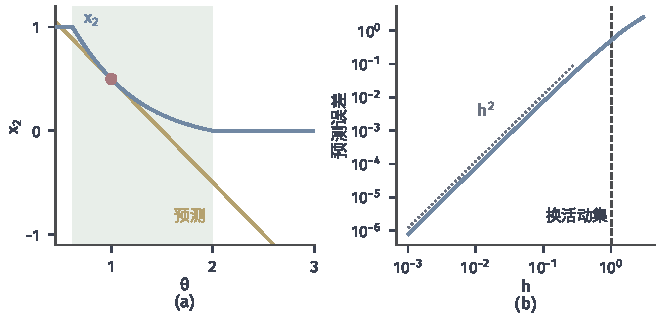
\includegraphics[width=112mm]{figures/05-optimization/06-constrained-optimization/matplotlib/sens-prediction-error/figure.pdf}
 \caption{价格例的一阶预测。(a)~$x_2(\theta)$的真实值（蓝线）和$\theta=1$处的线性预测（黄线），绿色区域是活动集保持的窗口。(b)~预测误差随$h$的变化（对数坐标，$\theta=1+h$），灰色点线是$h^2$的参考线，黑色虚线标出活动集改变的位置$h=1$。}
 \label{fig:sens-prediction-error}
\end{BookInlineFigure}

\section{本章小结}
\label{sec:sens-summary}

本章开头问：预算多一点，最优值变化多少，最优解往哪里移？回答这个问题，首先要说清比较的对象。最优值函数$V$是全局的，分支上的值$v$是局部的，解集合$\bm{S}$可能为空或含多个点，只有选定分支或选解规则才有“解的导数”可谈。

最优值的变化有两类结论。约束右端扰动时，零间隙且乘子达到就给出对任意大小的扰动都成立的仿射下界，它不要求凸性，也不要求活动集不变。只有在$V$可微时，下界的斜率才等于实际导数；$V$不可微时，全体最优乘子的相反数构成全部下界斜率，方向导数由其中最不利的一个决定。目标参数的变化由包络关系描述，一般含参约束下导数等于Lagrange函数显含参数的偏导。

最优解的移动由可逆的最优性方程描述。无约束时看Hessian，等式约束时看KKT矩阵，只需在切空间上正定。不等式约束再加上LICQ与严格互补，活动约束便可当作等式处理。隐函数定理给出的是局部结论，定理的条件是充分而非必要的，方程的光滑解也要用二阶条件判定是否极小。

这些局部结论的失效方式彼此不同。活动集改变时，解连续但转折，值函数可能仍然可微。全局最优解切换时，每条分支都光滑，全局值出现折角，解发生跳跃。方程退化时，唯一的解也可能没有有限的导数，而值函数依然可微。判别时要看的是可用的方程、所选的分支和线性方程的可逆性分别是否变化。

计算时，同一次$\bm{K}$分解可以服务多个右端，只要一个输出的梯度时伴随法只需一个右端。隐式导数对应精确的最优性方程，近似解、有限差分和有限次算法展开各自带有不同的误差，预测的有效性要靠余量、乘子符号和小幅重解来核验。第~\ref{chap:simplex-method}章的固定基分析正是这一思路在线性规划上的实例，第~\ref{chap:bilevel-optimization}章将继续用解映射的导数研究双层优化。


\chapter{二次规划与锥规划}
\label{chap:quadratic-conic-programming}

设三次观测告诉我们$x_1+x_2\approx4$、$x_1\approx1$、$x_2\approx0$，而$x_1,x_2$又必须非负、总和不超过$2$。这是带预算的最小二乘。换一个场合：要在两个圆盘的公共部分里找位置最低的点。再换一个：知道三个量两两之间的部分相关系数，要判断剩下的那个相关系数能取哪些值。

三件事看上去毫无关系，求解前却要回答同一个问题：目标和约束究竟是什么形状，能不能写成已有方法可以直接处理的形式？第一件事的目标是二次函数、约束是线性的；第二件事的约束是欧氏距离的上限；第三件事的约束是“某个对称矩阵的特征值非负”。这三种形状分别对应二次规划、二阶锥规划和半正定规划。

第~\ref{sec:cone-qp}节研究二次规划，看曲率和可行集怎样决定凸性、唯一性和计算方式。第~\ref{sec:cone-conic}节把线性规划的非负约束换成一般的闭凸锥，得到一种统一的模型和统一的对偶下界。

问题本身未必长成标准形式。第~\ref{sec:cone-rewrite}节研究怎样引入辅助变量而不改变问题，第~\ref{sec:cone-relax}节处理改不成凸问题的情形：放宽可行集，换来一个可以计算的下界。这两种操作的差别贯穿后半章，算出来的东西和原问题的关系也要分别核对。第~\ref{sec:cone-methods}节在同一个问题上比较各种写法的规模与代价。

\section{二次规划}
\label{sec:cone-qp}

拿到一个二次目标、线性约束的问题，于是要问：怎样在动手求解之前，判断它是否凸、解是否唯一、哪些线性代数运算可以直接拿来用？

\paragraph{从带预算的最小二乘开始}
回到章首的三次观测。把三条近似关系写成$\bm{D}\bm{x}\approx\bm{r}$，其中
\[
 \bm{D}=\begin{bmatrix}1&1\\1&0\\0&1\end{bmatrix},\qquad
 \bm{r}=\begin{bmatrix}4\\1\\0\end{bmatrix}.
\]
最小二乘的目标是$\frac12\lVert\bm{D}\bm{x}-\bm{r}\rVert_2^2$，约束是$\bm{x}\geq\bm{0}$和预算$x_1+x_2\leq2$。把这三条约束收集起来，就得到本节贯穿使用的问题。

展开平方，目标等于
\[
 \frac12\bm{x}^\top\bm{D}^\top\bm{D}\bm{x}-\bm{r}^\top\bm{D}\bm{x}+\frac12\lVert\bm{r}\rVert_2^2.
\]
常数项不影响最优解。记$\bm{Q}=\bm{D}^\top\bm{D}$、$\bm{q}=-\bm{D}^\top\bm{r}$，代入数据得到
\begin{equation}
 \bm{Q}=\begin{bmatrix}2&1\\1&2\end{bmatrix},\qquad
 \bm{q}=\begin{bmatrix}-5\\-4\end{bmatrix},\qquad
 \frac12\lVert\bm{r}\rVert_2^2=\frac{17}{2}.
 \label{eq:cone-running-data}
\end{equation}
于是目标是一个对称二次型加一个线性项，约束全是仿射的。

把这种形状抽象出来，就是下面的定义。为了不和最小二乘的$\bm{D},\bm{r}$混淆，约束的系数用另外的字母。

\begin{definition}[二次规划]
\label{def:cone-qp}
设$\bm{Q}\in\mathbb{R}^{n\times n}$对称，$\bm{q}\in\mathbb{R}^n$，$\bm{A}\in\mathbb{R}^{p\times n}$，$\bm{b}\in\mathbb{R}^p$，$\bm{G}\in\mathbb{R}^{m\times n}$，$\bm{h}\in\mathbb{R}^m$。问题
\begin{equation}
 \begin{aligned}
 \min_{\bm{x}\in\mathbb{R}^n}\quad&f(\bm{x})=\frac12\bm{x}^\top\bm{Q}\bm{x}+\bm{q}^\top\bm{x}\\
 \text{s.t.}\quad&\bm{A}\bm{x}=\bm{b},\quad\bm{G}\bm{x}\leq\bm{h}
 \end{aligned}
 \label{eq:cone-qp}
\end{equation}
称为\term{二次规划}（quadratic program，QP）。不等式逐分量理解。可行集$\bm{C}$是有限个闭半空间与超平面的交，即多面体。
\end{definition}

例中$p=0$，三条不等式对应
\[
 \bm{G}=\begin{bmatrix}1&1\\-1&0\\0&-1\end{bmatrix},\qquad
 \bm{h}=\begin{bmatrix}2\\0\\0\end{bmatrix}.
\]
若把预算换成每个分量各自的上下限$\bm{l}\leq\bm{x}\leq\bm{u}$，得到的是盒约束最小二乘，只是$\bm{G},\bm{h}$的内容不同，目标部分完全一样。

\paragraph{拿到二次规划先问三件事}
同一个形式~\eqref{eq:cone-qp}覆盖了难度相差极大的问题，差别由下面三件事决定。

\begin{enumerate}
 \item 曲率：$\bm{Q}$沿可以移动的方向是正、是零还是负？这决定问题是否凸、解是否唯一。
 \item 可行集：有哪些等式和不等式，集合是否有界？这决定解会不会落在边界上、会不会跑到无穷远。
 \item 线性代数结构：$\bm{Q}$和约束矩阵是否稀疏、是否已有分解？这决定一次计算要花多少。
\end{enumerate}

图~\ref{fig:cone-qp-budget}画出例子。蓝色椭圆是目标的等高线，中心$(2,1)$是不考虑约束时的最小二乘解。它的两个分量之和是$3$，超出预算，所以留在三角形内的最好位置落在预算边上。在解$\bm{x}^\star$处，负梯度仍然指向更低的椭圆中心，但沿这个方向走会离开可行集。

\begin{BookInlineFigure}
  \centering
  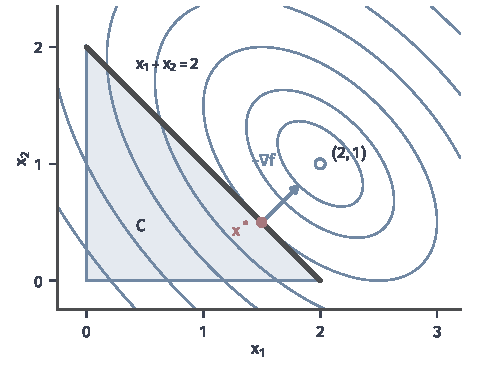
\includegraphics[width=84mm]{figures/05-optimization/06-constrained-optimization/matplotlib/cone-qp-budget/figure.pdf}
  \caption{带预算的最小二乘问题。蓝色椭圆是目标$\frac12\lVert\bm{D}\bm{x}-\bm{r}\rVert_2^2$的等高线，空心点$(2,1)$是无约束解。浅蓝三角形是可行集，深灰粗线是活动的预算约束，红点是解$\bm{x}^\star=(3/2,1/2)$。蓝色箭头是按比例缩短的负梯度，它垂直于预算边。}
  \label{fig:cone-qp-budget}
\end{BookInlineFigure}

\subsection{凸二次规划}
\label{sec:cone-convex-qp}

这一小节回答前两件事：目标在可行集上什么时候是一只碗，这只碗什么时候只有一个最低点。答案全部来自二次函数的一个恒等式。

\paragraph{一个恒等式}
二次函数的特别之处在于，它的高阶余项是零，局部信息就是全局信息。下面的引理把这句话写成精确的等式。

\begin{lemma}[二次函数的两个恒等式]
\label{lem:cone-quadratic-identities}
设$f$是式~\eqref{eq:cone-qp}中的二次函数，$\bm{Q}$对称。则$\nabla f(\bm{x})=\bm{Q}\bm{x}+\bm{q}$，且对任意$\bm{x},\bm{y}\in\mathbb{R}^n$和$\theta\in[0,1]$，
\begin{equation}
 f(\bm{y})=f(\bm{x})+\nabla f(\bm{x})^\top(\bm{y}-\bm{x})+\frac12(\bm{y}-\bm{x})^\top\bm{Q}(\bm{y}-\bm{x}),
 \label{eq:cone-exact-taylor}
\end{equation}
\begin{equation}
 \begin{aligned}
 f(\theta\bm{x}+(1-\theta)\bm{y})={}&\theta f(\bm{x})+(1-\theta)f(\bm{y})\\
 &-\frac12\theta(1-\theta)(\bm{x}-\bm{y})^\top\bm{Q}(\bm{x}-\bm{y}).
 \end{aligned}
 \label{eq:cone-chord-identity}
\end{equation}
\end{lemma}

\begin{proof}
记$\bm{d}=\bm{y}-\bm{x}$。直接展开，
\[
 f(\bm{x}+\bm{d})=\frac12\bm{x}^\top\bm{Q}\bm{x}+\bm{x}^\top\bm{Q}\bm{d}+\frac12\bm{d}^\top\bm{Q}\bm{d}+\bm{q}^\top\bm{x}+\bm{q}^\top\bm{d}.
\]
把含$\bm{d}$一次的两项合并成$(\bm{Q}\bm{x}+\bm{q})^\top\bm{d}$，就是式~\eqref{eq:cone-exact-taylor}。对$\bm{d}$的一次项系数就是梯度。

再证式~\eqref{eq:cone-chord-identity}。令$\bm{d}=\bm{x}-\bm{y}$，则$\theta\bm{x}+(1-\theta)\bm{y}=\bm{y}+\theta\bm{d}$。由式~\eqref{eq:cone-exact-taylor}，
\[
 f(\bm{y}+\theta\bm{d})=f(\bm{y})+\theta\nabla f(\bm{y})^\top\bm{d}+\frac12\theta^2\bm{d}^\top\bm{Q}\bm{d}.
\]
同一公式取步长$1$，得到
\[
 f(\bm{x})=f(\bm{y})+\nabla f(\bm{y})^\top\bm{d}+\frac12\bm{d}^\top\bm{Q}\bm{d}.
\]
于是
\[
 \theta f(\bm{x})+(1-\theta)f(\bm{y})=f(\bm{y})+\theta\nabla f(\bm{y})^\top\bm{d}+\frac12\theta\bm{d}^\top\bm{Q}\bm{d}.
\]
两式相减，差等于$\frac12(\theta^2-\theta)\bm{d}^\top\bm{Q}\bm{d}$，即式~\eqref{eq:cone-chord-identity}最后一项。
\end{proof}

式~\eqref{eq:cone-chord-identity}说，弦上的点比弦下面的函数值高出多少，完全由$(\bm{x}-\bm{y})^\top\bm{Q}(\bm{x}-\bm{y})$决定。线性项在其中不起作用。这一项为正，函数在这条线段上向下弯成碗；为负，则向上拱起。

因此要判断凸性，只需要看$\bm{Q}$在所有“两个可行点之差”上的符号。方向若永远走不到，它的曲率再负也无妨。

\paragraph{只看可行差方向}
把可行差张成的子空间记为
\begin{equation}
 \bm{V}=\operatorname{span}\{\bm{x}-\bm{y}:\bm{x},\bm{y}\in\bm{C}\},
 \label{eq:cone-feasible-subspace}
\end{equation}
并取$\bm{Z}$为一个矩阵，其各列构成$\bm{V}$的基。若$\bm{C}$中存在严格满足全部不等式的点，且$\bm{A}$的约束相容，则$\bm{V}=\ker\bm{A}$；此时$\bm{Z}$就是$\bm{A}$的零空间基。矩阵$\bm{Z}^\top\bm{Q}\bm{Z}$记录了$\bm{Q}$在可行方向上的全部曲率。

\begin{theorem}[可行集上的凸性]
\label{thm:cone-feasible-convexity}
设$\bm{C}$是式~\eqref{eq:cone-qp}的非空可行集，$\bm{Z}$的各列是$\bm{V}$的基。则
\begin{enumerate}
 \item $f$在$\bm{C}$上凸，当且仅当$\bm{Z}^\top\bm{Q}\bm{Z}\succeq\bm{0}$；
 \item $f$在$\bm{C}$上严格凸，当且仅当$\bm{Z}^\top\bm{Q}\bm{Z}\succ\bm{0}$。
\end{enumerate}
特别地，$\bm{Q}\succeq\bm{0}$时$f$在任何凸集上都凸。
\end{theorem}

\begin{proof}
先说明可行差足以探测$\bm{V}$中的每个方向。非空凸集在它的仿射包内有内点，取这样一个点$\bar{\bm{x}}$。存在$\varepsilon>0$，使得对$\bm{V}$中满足$\lVert\bm{d}\rVert_2\leq\varepsilon$的$\bm{d}$，都有$\bar{\bm{x}}+\bm{d}\in\bm{C}$。所以这样的$\bm{d}$是可行差，$\bm{V}$中任一非零方向乘上适当的正数后都是可行差。

设$f$在$\bm{C}$上凸。对$\bm{x}=\bar{\bm{x}}+\bm{d}$和$\bm{y}=\bar{\bm{x}}$，式~\eqref{eq:cone-chord-identity}中的最后一项必须不为正，故$\bm{d}^\top\bm{Q}\bm{d}\geq0$。缩放后对$\bm{V}$中全部方向成立，这就是$\bm{Z}^\top\bm{Q}\bm{Z}\succeq\bm{0}$。

反过来，若$\bm{Z}^\top\bm{Q}\bm{Z}\succeq\bm{0}$，则对任意$\bm{x},\bm{y}\in\bm{C}$，$\bm{x}-\bm{y}\in\bm{V}$，式~\eqref{eq:cone-chord-identity}中的最后一项不为正，$f$在$\bm{C}$上凸。

严格凸的情形相同。取$\bm{x}\neq\bm{y}$和$\theta\in(0,1)$，式~\eqref{eq:cone-chord-identity}说明弦严格高于函数，当且仅当$(\bm{x}-\bm{y})^\top\bm{Q}(\bm{x}-\bm{y})>0$。把上面两段的非负换成严格为正，论证逐句成立。
\end{proof}

最小二乘天然满足定理的条件。对$\bm{Q}=\bm{D}^\top\bm{D}$，有
\[
 \bm{d}^\top\bm{Q}\bm{d}=\lVert\bm{D}\bm{d}\rVert_2^2\geq0.
\]
所以带线性约束的最小二乘总是凸二次规划。严格凸与否取决于$\ker\bm{D}$与$\bm{V}$是否只交于零向量。例中$\bm{D}$列满秩，$\bm{Q}$的特征值是$1$和$3$，全空间正定。

\paragraph{连接线性方程与最优性条件}
没有约束时，最优条件是$\bm{Q}\bm{x}+\bm{q}=\bm{0}$，也就是最小二乘的正规方程$\bm{D}^\top\bm{D}\bm{x}=\bm{D}^\top\bm{r}$，其解法和选解可参考\BookChapterRef{chap:linear-solution-selection}{卷二第11章“线性方程与最小二乘的选解”}。例中由式~\eqref{eq:cone-running-data}解得无约束解$(2,1)$。

加上约束后，方程要换成第~\ref{chap:constrained-optimality}章的KKT条件。那一章证明了：约束全是仿射函数时，局部极小点满足KKT条件，不需要额外的约束规格。对问题~\eqref{eq:cone-qp}，KKT条件写成存在$\bm{\lambda}\in\mathbb{R}^m$和$\bm{\nu}\in\mathbb{R}^p$，使得
\begin{equation}
 \begin{gathered}
 \bm{Q}\bm{x}+\bm{q}+\bm{A}^\top\bm{\nu}+\bm{G}^\top\bm{\lambda}=\bm{0},\\
 \bm{A}\bm{x}=\bm{b},\qquad\bm{G}\bm{x}\leq\bm{h},\\
 \bm{\lambda}\geq\bm{0},\qquad\bm{\lambda}^\top(\bm{G}\bm{x}-\bm{h})=0.
 \end{gathered}
 \label{eq:cone-qp-kkt}
\end{equation}

凸性让这组条件从必要变成充分，也就成了全局最优的证书。

\begin{theorem}[凸二次规划的KKT证书]
\label{thm:cone-qp-kkt}
设$f$在$\bm{C}$上凸。可行点$\bm{x}$是问题~\eqref{eq:cone-qp}的全局最优解，当且仅当存在$\bm{\lambda},\bm{\nu}$使式~\eqref{eq:cone-qp-kkt}成立。
\end{theorem}

\begin{proof}
必要性是上面复述的结论，全局最优解当然是局部极小点。下面证充分性。任取可行点$\bm{y}$，记$\bm{d}=\bm{y}-\bm{x}$。由式~\eqref{eq:cone-exact-taylor}，
\[
 f(\bm{y})-f(\bm{x})=\nabla f(\bm{x})^\top\bm{d}+\frac12\bm{d}^\top\bm{Q}\bm{d}.
\]
$\bm{d}$是可行差，定理~\ref{thm:cone-feasible-convexity}给出$\bm{d}^\top\bm{Q}\bm{d}\geq0$。只需证第一项非负。

把驻定条件代入，并用$\bm{A}\bm{d}=\bm{0}$，得到
\[
 \nabla f(\bm{x})^\top\bm{d}=-\bm{\nu}^\top\bm{A}\bm{d}-\bm{\lambda}^\top\bm{G}\bm{d}=-\bm{\lambda}^\top\bm{G}\bm{d}.
\]
由互补条件$\bm{\lambda}^\top(\bm{G}\bm{x}-\bm{h})=0$，上式可以写成
\[
 -\bm{\lambda}^\top\bm{G}\bm{d}=-\bm{\lambda}^\top(\bm{G}\bm{y}-\bm{h})+\bm{\lambda}^\top(\bm{G}\bm{x}-\bm{h})=-\bm{\lambda}^\top(\bm{G}\bm{y}-\bm{h}).
\]
$\bm{\lambda}\geq\bm{0}$且$\bm{G}\bm{y}\leq\bm{h}$，所以右端非负。于是$f(\bm{y})\geq f(\bm{x})$。
\end{proof}

这个证书的好处是核对便宜。给出$\bm{x}$和$\bm{\lambda}$，只需做几次矩阵乘法，不必重新求解。

\begin{example}[核对预算问题的解]
\label{ex:cone-qp-kkt}
猜测预算活动、非负约束不活动。可行点$(3/2,1/2)$如何得来，下一小节再算，这里先核对。由式~\eqref{eq:cone-running-data}，
\[
 \nabla f(\bm{x})=\bm{Q}\bm{x}+\bm{q}=\begin{bmatrix}7/2\\5/2\end{bmatrix}+\begin{bmatrix}-5\\-4\end{bmatrix}=\begin{bmatrix}-3/2\\-3/2\end{bmatrix}.
\]
取$\bm{\lambda}=(3/2,0,0)$，则
\[
 \nabla f(\bm{x})+\bm{G}^\top\bm{\lambda}=\begin{bmatrix}-3/2\\-3/2\end{bmatrix}+\frac32\begin{bmatrix}1\\1\end{bmatrix}=\bm{0}.
\]
互补条件成立，因为预算的松弛量是$0$，另外两条约束的乘子是$0$。$\bm{\lambda}\geq\bm{0}$也成立。由定理~\ref{thm:cone-qp-kkt}，$(3/2,1/2)$是全局最优解。

最优值按$\frac12\lVert\bm{D}\bm{x}-\bm{r}\rVert_2^2$计算。残差是$\bm{D}\bm{x}-\bm{r}=(-2,1/2,1/2)$，于是
\[
 f^\star=\frac12\Bigl(4+\frac14+\frac14\Bigr)=\frac94.
\]
\end{example}

\paragraph{解的存在与唯一}
凸性不保证最优解存在。$\frac12x_1^2+x_2$的$\bm{Q}$半正定，在全平面上却无下界，沿$x_2\to-\infty$一路下降。有下界时情况好得多：二次函数只要在非空多面体上有下界，就一定取得最小值。这一结论称为Frank--Wolfe定理，它不要求凸性；证明要对约束个数作归纳，处理最小化序列沿回收方向发散的情形，篇幅较长，读者可查阅二次规划方面的专著。

这里有一点值得和一般光滑函数对比。第~\ref{chap:optimization}章的$e^x$在全直线上有下界$0$，却取不到。二次函数不会有这样的渐近行为。

唯一性由曲率直接给出，而且只需要看可行差方向。

\begin{theorem}[存在唯一性的充分条件]
\label{thm:cone-qp-unique}
设$\bm{C}$非空，且对$\bm{V}$中每个非零$\bm{d}$都有$\bm{d}^\top\bm{Q}\bm{d}>0$。则问题~\eqref{eq:cone-qp}恰有一个最优解。
\end{theorem}

\begin{proof}
先证存在。取$\bar{\bm{x}}\in\bm{C}$，$\bm{C}$中的点都可写成$\bar{\bm{x}}+\bm{Z}\bm{u}$。此时$f$成为$\bm{u}$的二次函数，其二次项矩阵$\bm{Z}^\top\bm{Q}\bm{Z}$正定，故$\lVert\bm{u}\rVert_2\to\infty$时函数值趋于$+\infty$，下水平集有界。可行集是闭集，所以下水平集紧，第~\ref{chap:optimization}章的存在定理给出最优解。

再证唯一。设$\bm{x}\neq\bm{y}$都是最优解，中点$\bm{z}=(\bm{x}+\bm{y})/2$可行。对式~\eqref{eq:cone-chord-identity}取$\theta=1/2$，并记$\bm{d}=\bm{x}-\bm{y}\in\bm{V}$，得到
\[
 f(\bm{z})=f^\star-\frac18\bm{d}^\top\bm{Q}\bm{d}<f^\star.
\]
这与$f^\star$是最优值矛盾。
\end{proof}

定理要求的是$\bm{V}$上正定，不是全空间正定。图~\ref{fig:cone-qp-uniqueness}比较了三种情形。

\begin{BookInlineFigure}
  \centering
  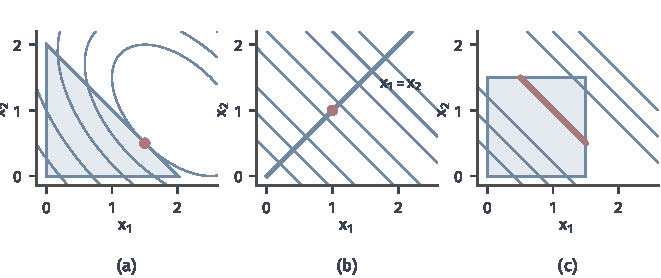
\includegraphics[width=112mm]{figures/05-optimization/06-constrained-optimization/matplotlib/cone-qp-uniqueness/figure.pdf}
  \caption{曲率与解的唯一性，蓝线是目标等高线，红色是解集。(a)预算问题，$\bm{Q}$全空间正定，解唯一。(b)目标$\frac12(x_1+x_2-2)^2$的$\bm{Q}$奇异，等高线是平行直线；约束直线$x_1=x_2$与谷底方向横截，解唯一。(c)同一目标，可行集是正方形$[0,3/2]^2$，平坦方向$(1,-1)$落在可行差内，解集是一条线段。}
  \label{fig:cone-qp-uniqueness}
\end{BookInlineFigure}

(b)中的目标来自只有一次观测的最小二乘，$\bm{D}=\begin{bmatrix}1&1\end{bmatrix}$，$\bm{r}=(2)$，于是$\bm{Q}=\begin{bmatrix}1&1\\1&1\end{bmatrix}$奇异，其零空间由$(1,-1)$张成。约束$x_1=x_2$使$\bm{V}$由$(1,1)$张成，而
\[
 (1,1)\,\bm{Q}\,(1,1)^\top=4>0.
\]
所以在可行直线上目标严格凸，解$(1,1)$唯一。全空间正定不是必要条件。

(c)中可行集仍是平面区域，平坦方向$(1,-1)$属于$\bm{V}$，定理的条件不成立，结论也确实不成立：线段$x_1+x_2=2$上的点全部最优，目标值都是$0$。

$\bm{V}$上正定同样不是唯一性的必要条件。考虑$\frac12x_1^2+x_2$，约束$x_2\geq0$。这里$\bm{V}=\mathbb{R}^2$，方向$(0,1)$的曲率为零，但线性项把解推到边界上：目标在可行集上非负，且只在原点为零，解唯一。线性规划是更极端的情形，$\bm{Q}=\bm{0}$，解却常常是唯一的顶点。

\paragraph{解集与可复用的运算}
凸二次规划的解不唯一时，解集也有规律。设$\bm{x},\bm{y}$都最优，式~\eqref{eq:cone-chord-identity}迫使$\bm{d}^\top\bm{Q}\bm{d}=0$，其中$\bm{d}=\bm{x}-\bm{y}$。$\bm{Q}\succeq\bm{0}$时这又推出$\bm{Q}\bm{d}=\bm{0}$，所以各最优解的梯度相同。解集上变的只有沿平坦方向的位置，不变的是梯度和最优值。

至于第三件事，二次规划的计算几乎都落到线性方程上。$\bm{Q}=\bm{D}^\top\bm{D}$时，$\bm{D}$的QR分解可以反复使用；求解过程换一组活动约束时，只需更新分解，不必重做。求解的形式与代价要到不等式的处理方法确定后才能比较，下一小节先看只有等式的情形。

\subsection{等式约束二次问题}
\label{sec:cone-equality-qp}

假如已经知道哪些不等式在解处活动，把它们当作等式，问题就只剩等式约束。这一小节研究
\begin{equation}
 \min_{\bm{x}}\ \frac12\bm{x}^\top\bm{Q}\bm{x}+\bm{q}^\top\bm{x}\quad\text{s.t.}\quad\bm{A}\bm{x}=\bm{b},
 \label{eq:cone-eqp}
\end{equation}
其中$\bm{A}\in\mathbb{R}^{p\times n}$行满秩，$p<n$。要回答的问题是：它能否化成一次线性方程，什么时候这个方程给出的确实是极小点？

例子取预算恰好用完的情形：$\bm{A}=\begin{bmatrix}1&1\end{bmatrix}$，$b=2$，$\bm{Q},\bm{q}$如式~\eqref{eq:cone-running-data}。可行集是平面上的一条直线。

可行集是一张平的“纸”，有两种自然的处理方式。一种是在纸上另取坐标，把问题变成无约束问题，只看纸面上的碗。另一种是留在原坐标里，引入乘子，把“不许离开纸面”变成方程。

\paragraph{零空间参数化}
取一个特解$\bm{x}_{\mathrm{p}}$满足$\bm{A}\bm{x}_{\mathrm{p}}=\bm{b}$，取$\bm{Z}\in\mathbb{R}^{n\times(n-p)}$，其各列是$\ker\bm{A}$的基。每个可行点都唯一地写成
\begin{equation}
 \bm{x}=\bm{x}_{\mathrm{p}}+\bm{Z}\bm{u},\qquad\bm{u}\in\mathbb{R}^{n-p}.
 \label{eq:cone-nullspace-param}
\end{equation}
约束被消去，$\bm{u}$可以取任意值。

把式~\eqref{eq:cone-nullspace-param}代入目标，并用式~\eqref{eq:cone-exact-taylor}以$\bm{x}_{\mathrm{p}}$为中心展开，得到$\bm{u}$的二次函数
\begin{equation}
 \varphi(\bm{u})=f(\bm{x}_{\mathrm{p}})+\bigl(\bm{Z}^\top(\bm{Q}\bm{x}_{\mathrm{p}}+\bm{q})\bigr)^\top\bm{u}+\frac12\bm{u}^\top\bm{Z}^\top\bm{Q}\bm{Z}\bm{u}.
 \label{eq:cone-reduced-objective}
\end{equation}
矩阵$\bm{Z}^\top\bm{Q}\bm{Z}$称为\term{约化Hessian}（reduced Hessian），它是目标在纸面上的曲率。令梯度为零，得到约化方程
\begin{equation}
 \bm{Z}^\top\bm{Q}\bm{Z}\,\bm{u}=-\bm{Z}^\top(\bm{Q}\bm{x}_{\mathrm{p}}+\bm{q}).
 \label{eq:cone-reduced-equation}
\end{equation}

在例子中取特解$\bm{x}_{\mathrm{p}}=(2,0)$和方向$\bm{z}=(1,-1)$。约化Hessian是一个数：
\[
 \bm{z}^\top\bm{Q}\bm{z}=2-1-1+2=2.
\]
$\bm{x}_{\mathrm{p}}$处的梯度是
\[
 \bm{Q}\bm{x}_{\mathrm{p}}+\bm{q}=\begin{bmatrix}4\\2\end{bmatrix}+\begin{bmatrix}-5\\-4\end{bmatrix}=\begin{bmatrix}-1\\-2\end{bmatrix}.
\]
它在$\bm{z}$上的投影是$\bm{z}^\top(\bm{Q}\bm{x}_{\mathrm{p}}+\bm{q})=1$。把两个数代入式~\eqref{eq:cone-reduced-equation}，得到
\[
 2u=-1,\qquad u^\star=-\frac12.
\]
于是
\[
 \bm{x}^\star=\begin{bmatrix}2\\0\end{bmatrix}-\frac12\begin{bmatrix}1\\-1\end{bmatrix}=\begin{bmatrix}3/2\\1/2\end{bmatrix}.
\]
这个点的两个分量都是正的，所以它也满足原来的非负约束，这正是例~\ref{ex:cone-qp-kkt}核对过的解。

图~\ref{fig:cone-qp-nullspace}(b)画出约化后的一元函数$\varphi(u)=u^2+u+5/2$。原问题的约束已经不见了，剩下的是一个普通的抛物线。

\begin{BookInlineFigure}
  \centering
  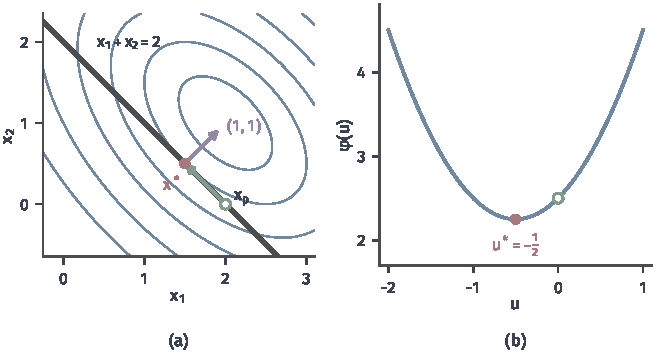
\includegraphics[width=112mm]{figures/05-optimization/06-constrained-optimization/matplotlib/cone-qp-nullspace/figure.pdf}
  \caption{预算恰好用完时的二次问题。(a)深灰粗线是可行直线，蓝线是目标等高线。从特解$\bm{x}_{\mathrm{p}}=(2,0)$（绿色空心点）沿零空间方向走到解（红点），绿色箭头是位移$u^\star\bm{z}$。紫色箭头是约束的法向$(1,1)$，解处的等高线与直线相切，梯度沿这个方向。(b)沿直线的一元函数$\varphi(u)=u^2+u+5/2$，空心点和红点对应(a)中的$\bm{x}_{\mathrm{p}}$与解。}
  \label{fig:cone-qp-nullspace}
\end{BookInlineFigure}

\paragraph{带乘子的块线性方程}
第二种做法不换坐标。对式~\eqref{eq:cone-eqp}写KKT条件，没有不等式，式~\eqref{eq:cone-qp-kkt}只剩两行，它们都是线性的。写成块形式：
\begin{equation}
 \begin{bmatrix}\bm{Q}&\bm{A}^\top\\\bm{A}&\bm{0}\end{bmatrix}
 \begin{bmatrix}\bm{x}\\\bm{\nu}\end{bmatrix}
 =\begin{bmatrix}-\bm{q}\\\bm{b}\end{bmatrix}.
 \label{eq:cone-kkt-system}
\end{equation}
左端的矩阵称为\term{KKT矩阵}（KKT matrix）。它对称，但不定，下方块是零。

例中方程组是
\[
 \begin{bmatrix}2&1&1\\1&2&1\\1&1&0\end{bmatrix}
 \begin{bmatrix}x_1\\x_2\\\nu\end{bmatrix}
 =\begin{bmatrix}5\\4\\2\end{bmatrix}.
\]
前两行相减消去$\nu$，得到$x_1-x_2=1$。第三行给出$x_1+x_2=2$。两式联立，
\[
 x_1=\frac32,\qquad x_2=\frac12.
\]
再代回第一行，
\[
 \nu=5-2x_1-x_2=\frac32.
\]
得到的$\bm{x}$与零空间参数化相同，还多了一个乘子。乘子的含义是预算的影子价格：预算增加一点点，最优值约按$\nu$的速率下降，这种变化率的一般讨论在第~\ref{chap:parametric-sensitivity}章。

两种做法解的是同一组条件。约束$\bm{A}\bm{x}=\bm{b}$由参数化自动满足，而$\ker\bm{A}$的正交补是$\bm{A}^\top$的列空间，所以下面两件事等价：
\begin{equation}
 \bm{Q}\bm{x}+\bm{q}\in\operatorname{range}(\bm{A}^\top)
 \quad\Longleftrightarrow\quad
 \bm{Z}^\top(\bm{Q}\bm{x}+\bm{q})=\bm{0}.
 \label{eq:cone-kkt-reduced-equivalence}
\end{equation}
左边是块方程第一行“存在$\bm{\nu}$”的说法，右边代入式~\eqref{eq:cone-nullspace-param}就是约化方程。

表~\ref{tab:cone-eqp-compare}比较两种做法的计算任务。

\begin{BookInlineTable}
  \centering
  \begin{tabular}{lll}
    \toprule
    & 零空间参数化 & 块线性方程\\
    \midrule
    需要准备 & 特解与零空间基$\bm{Z}$ & 无\\
    解的方程 & $(n-p)$阶，常可用Cholesky & $(n+p)$阶，对称不定\\
    适合的情形 & $n-p$小，$\bm{Z}$易得 & $\bm{Q}$、$\bm{A}$稀疏\\
    副产品 & 乘子需另算 & 直接得到乘子\\
    \bottomrule
  \end{tabular}
  \caption{等式约束二次问题的两种解法。$\bm{Z}$通常来自$\bm{A}^\top$的QR分解，$\bm{Q}$、$\bm{A}$稀疏时$\bm{Z}$和$\bm{Z}^\top\bm{Q}\bm{Z}$可能变稠密。}
  \label{tab:cone-eqp-compare}
\end{BookInlineTable}

\paragraph{唯一可解的条件}
块方程什么时候有唯一解？式~\eqref{eq:cone-kkt-reduced-equivalence}提示答案取决于约化Hessian，而不是$\bm{Q}$本身。

\begin{theorem}[KKT矩阵的可逆性]
\label{thm:cone-kkt-invertible}
设$\bm{A}\in\mathbb{R}^{p\times n}$行满秩，$\bm{Z}$的各列是$\ker\bm{A}$的基。则
\begin{enumerate}
 \item KKT矩阵可逆，当且仅当$\bm{Z}^\top\bm{Q}\bm{Z}$可逆；
 \item 若$\bm{Z}^\top\bm{Q}\bm{Z}\succ\bm{0}$，则式~\eqref{eq:cone-kkt-system}有唯一解，其中的$\bm{x}$是问题~\eqref{eq:cone-eqp}唯一的全局最优解。
\end{enumerate}
\end{theorem}

\begin{proof}
设$(\bm{d},\bm{w})$在KKT矩阵的零空间中，即
\[
 \bm{Q}\bm{d}+\bm{A}^\top\bm{w}=\bm{0},\qquad\bm{A}\bm{d}=\bm{0}.
\]
由第二式可写$\bm{d}=\bm{Z}\bm{u}$。第一式左乘$\bm{Z}^\top$，因为$\bm{A}\bm{Z}=\bm{0}$，得到$\bm{Z}^\top\bm{Q}\bm{Z}\bm{u}=\bm{0}$。

若$\bm{Z}^\top\bm{Q}\bm{Z}$可逆，则$\bm{u}=\bm{0}$，$\bm{d}=\bm{0}$。此时第一式成为$\bm{A}^\top\bm{w}=\bm{0}$，$\bm{A}$行满秩推出$\bm{w}=\bm{0}$。所以KKT矩阵可逆。

反过来，若存在$\bm{u}\neq\bm{0}$使$\bm{Z}^\top\bm{Q}\bm{Z}\bm{u}=\bm{0}$，令$\bm{d}=\bm{Z}\bm{u}\neq\bm{0}$。则$\bm{Q}\bm{d}$与$\ker\bm{A}$正交，属于$\operatorname{range}(\bm{A}^\top)$，存在$\bm{w}$使$\bm{Q}\bm{d}+\bm{A}^\top\bm{w}=\bm{0}$。$(\bm{d},\bm{w})$是非零的零空间向量，KKT矩阵奇异。第一条得证。

第二条的可逆性由第一条给出。此时$\varphi$严格凸，其唯一驻点是唯一的全局极小点；由式~\eqref{eq:cone-kkt-reduced-equivalence}，这个驻点正是块方程解中的$\bm{x}$。
\end{proof}

定理中的“行满秩”也是必需的。若$\bm{A}$行亏秩，存在$\bm{w}\neq\bm{0}$使$\bm{A}^\top\bm{w}=\bm{0}$，$(\bm{0},\bm{w})$就在零空间里，块方程要么无解，要么乘子不唯一。

\paragraph{可逆不等于极小}
线性方程组非奇异，只说明驻点存在且唯一，并不说明驻点是极小点。第一条与第二条之间差的正是约化曲率的符号。

取$\bm{Q}=\operatorname{diag}(1,-1)$，$\bm{q}=\bm{0}$，约束是过原点的直线，方向为$\bm{z}$。图~\ref{fig:cone-qp-reduced}比较了三个方向。目标沿直线$\bm{x}=s\bm{z}$的值是$\frac12s^2\bm{z}^\top\bm{Q}\bm{z}$，约化Hessian就是数$\bm{z}^\top\bm{Q}\bm{z}$。

\begin{BookInlineFigure}
  \centering
  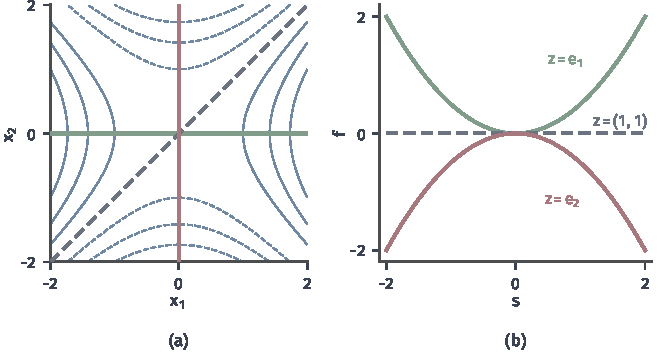
\includegraphics[width=112mm]{figures/05-optimization/06-constrained-optimization/matplotlib/cone-qp-reduced/figure.pdf}
  \caption{约化曲率决定驻点的性质。目标$\frac12(x_1^2-x_2^2)$，$\bm{q}=\bm{0}$。(a)蓝线是等高线（实线为正值，虚线为负值），三条直线是过原点的可行集。(b)目标沿每条直线的取值，横轴是直线上的坐标。绿线的约化曲率为$1$，灰色虚线为$0$，红线为$-1$。}
  \label{fig:cone-qp-reduced}
\end{BookInlineFigure}

表~\ref{tab:cone-reduced-cases}列出三种结果。

\begin{BookInlineTable}
  \centering
  \begin{tabular}{llll}
    \toprule
    方向$\bm{z}$ & $\bm{z}^\top\bm{Q}\bm{z}$ & KKT矩阵 & 原点的性质\\
    \midrule
    $(1,0)$ & $1$ & 可逆 & 唯一全局极小点\\
    $(1,1)$ & $0$ & 奇异 & 整条直线都是驻点\\
    $(0,1)$ & $-1$ & 可逆 & 沿直线的极大点，问题无下界\\
    \bottomrule
  \end{tabular}
  \caption{$\bm{Q}=\operatorname{diag}(1,-1)$、$\bm{q}=\bm{0}$时，约束直线的方向决定KKT矩阵和驻点的性质。}
  \label{tab:cone-reduced-cases}
\end{BookInlineTable}

第三行是要警惕的情形。此时约束是$x_1=0$，$\bm{A}=\begin{bmatrix}1&0\end{bmatrix}$，块方程的矩阵
\[
 \begin{bmatrix}1&0&1\\0&-1&0\\1&0&0\end{bmatrix}
\]
行列式为$1$，可逆，解是$\bm{x}=\bm{0}$、$\nu=0$。求解器不会报告任何异常，但$(0,s)$处的目标是$-\frac12s^2$，$\bm{x}=\bm{0}$是沿可行直线的最高点。

所以解完块方程还要核对约化曲率。不想构造$\bm{Z}$时可以看KKT矩阵的惯性：$\bm{A}$行满秩时，KKT矩阵恰有$n$个正特征值、$p$个负特征值，当且仅当$\bm{Z}^\top\bm{Q}\bm{Z}\succ\bm{0}$，而对称不定分解能直接读出惯性\scite{math-nocedal2006numerical}。

含不等式时，还要决定哪些不等式按等式处理，这个选择问题以及逐步调整的求解方法在第~\ref{chap:sequential-quadratic-programming}章展开。

\subsection{非凸二次问题}
\label{sec:cone-nonconvex-qp}

$\bm{Q}$在可行差方向上有负曲率时，前面的两个定理都不能用。这一小节要弄清：负曲率到底造成什么后果，约束又能挽回多少？

\paragraph{一个负曲率的例子}
考虑$\bm{Q}=\operatorname{diag}(1,-1)$的目标
\begin{equation}
 f(\bm{x})=\frac12x_1^2-\frac12x_2^2+\frac14x_2.
 \label{eq:cone-nonconvex-objective}
\end{equation}
沿$x_1$方向是碗，沿$x_2$方向是倒扣的碗。

先不加约束。唯一的驻点由$x_1=0$和$-x_2+\frac14=0$给出，是$\mathrm{S}=(0,1/4)$。沿$x_2$方向走，目标趋于$-\infty$，所以这个问题无下界，驻点是鞍点。

现在加上$-1\leq x_2\leq1$。约束切断了$x_2$方向的无限下降，$x_1$方向的目标又非负，所以目标在可行集上有下界。这就是图~\ref{fig:cone-qp-nonconvex}(a)中的带形区域。

\begin{BookInlineFigure}
  \centering
  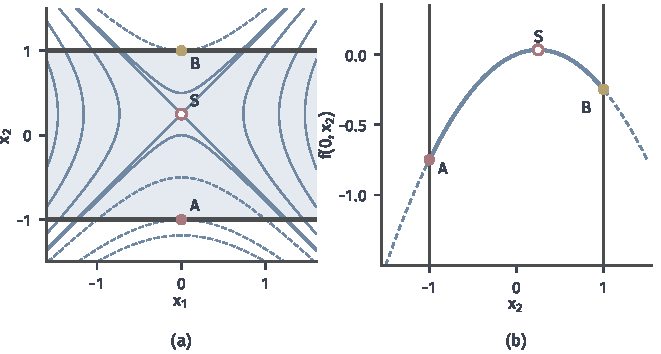
\includegraphics[width=112mm]{figures/05-optimization/06-constrained-optimization/matplotlib/cone-qp-nonconvex/figure.pdf}
  \caption{非凸二次问题的三个KKT点。目标$\frac12x_1^2-\frac12x_2^2+\frac14x_2$，可行集$-1\leq x_2\leq1$。(a)浅蓝带形是可行集，深灰粗线是约束边界，蓝线是等高线（虚线为负的较低水平）。红色实心点A是全局极小点，黄点B是局部极小点，红色空心点S是鞍点。(b)沿$x_1=0$的目标值，两条竖线之外不可行（虚线）。}
  \label{fig:cone-qp-nonconvex}
\end{BookInlineFigure}

\paragraph{KKT点的逐个判别}
约束写成$x_2-1\leq0$和$-x_2-1\leq0$，乘子分别记$\lambda_1,\lambda_2$。驻定条件给出$x_1=0$，以及
\[
 -x_2+\frac14+\lambda_1-\lambda_2=0.
\]
两条约束不能同时活动，所以按活动约束只有三种情形，每一种都是一个线性方程，结果列在表~\ref{tab:cone-nonconvex-kkt}中。

\begin{BookInlineTable}
  \centering
  \begin{tabular}{llll}
    \toprule
    点 & 活动约束 & 乘子 & 目标值\\
    \midrule
    $\mathrm{A}=(0,-1)$ & $x_2\geq-1$ & $\lambda_2=5/4$ & $-3/4$\\
    $\mathrm{B}=(0,1)$ & $x_2\leq1$ & $\lambda_1=3/4$ & $-1/4$\\
    $\mathrm{S}=(0,1/4)$ & 无 & $0$ & $1/32$\\
    \bottomrule
  \end{tabular}
  \caption{目标~\eqref{eq:cone-nonconvex-objective}在带形可行集上的三个KKT点。}
  \label{tab:cone-nonconvex-kkt}
\end{BookInlineTable}

三个点都满足一阶条件，性质却各不相同。判别要用第~\ref{chap:constrained-optimality}章的二阶条件：在乘子为正的活动约束的切方向上看曲率。

在A和B处，活动约束的乘子都为正，临界方向只有$(d_1,0)$，曲率$d_1^2>0$，所以二者都是严格局部极小点。在S处没有活动约束，$\bm{Q}$本身不定，沿$(0,1)$的曲率为负，所以S是鞍点。

比较目标值，A是全局极小点，B只是局部极小点。

\paragraph{不能继承的全局证书}
B满足全部KKT条件，却不是全局最优解。定理~\ref{thm:cone-qp-kkt}的证明在这里断在哪一步？取$\bm{x}=\mathrm{B}$、$\bm{y}=\mathrm{A}$，$\bm{d}=(0,-2)$。式~\eqref{eq:cone-exact-taylor}的两部分分别是
\[
 \nabla f(\mathrm{B})^\top\bm{d}=\Bigl(-\frac34\Bigr)(-2)=\frac32,\qquad
 \frac12\bm{d}^\top\bm{Q}\bm{d}=-2.
\]
一阶部分依然非负，这是KKT条件保证的。但二次部分为负，而且绝对值更大，两者之和是$-1/2$，恰好等于$f(\mathrm{A})-f(\mathrm{B})$。

表~\ref{tab:cone-nonconvex-feasible}把局部最优、鞍点和无下界并列起来。若只保留上界$x_2\leq1$、去掉下界，B依然是严格局部极小点，问题却变成无下界。局部信息看不出全局的命运。

\begin{BookInlineTable}
  \centering
  \begin{tabular}{lll}
    \toprule
    可行集 & 负曲率方向 & 结论\\
    \midrule
    全平面 & 不受限制 & 无下界，S是鞍点\\
    $x_2\leq1$ & 只能向下走 & B局部极小，问题无下界\\
    $-1\leq x_2\leq1$ & 被两侧截断 & A全局极小，B局部极小，S鞍点\\
    $x_2=0$ & 被完全禁止 & 约化后严格凸，解唯一\\
    \bottomrule
  \end{tabular}
  \caption{同一目标~\eqref{eq:cone-nonconvex-objective}在不同可行集上的结果。约束可以限制负曲率方向，但限制的方式决定结论。}
  \label{tab:cone-nonconvex-feasible}
\end{BookInlineTable}

\paragraph{局部解的数量}
局部极小点可以非常多。在盒$[-1,1]^n$上最小化$-\frac12\lVert\bm{x}\rVert_2^2$，每个顶点都是严格局部极小点，共$2^n$个，且每个都满足KKT条件。一般非凸二次规划的全局求解是NP困难问题，这个结论的证明需要计算复杂性理论的归约，这里只用它说明：不能指望靠逐个检查KKT点解决大规模问题。

不过二次结构并没有消失。梯度仍是线性的，每猜一组活动约束仍只需解一次线性方程，局部极小点仍可以用迭代方法找到。缺的是一个能断言“再也找不到更好的点”的全局依据。第~\ref{sec:cone-relax}节将给出另一类下界，用来补上这个缺口。

\section{锥规划}
\label{sec:cone-conic}

二次规划的约束仍是平的，可行集的边界由超平面拼成。距离上限、矩阵半正定这样的条件却给出弯曲的边界。接下来要弄清：怎样把这些弯曲的约束放进一个共同的形式，同时保留线性规划那种“任何人都能核对”的对偶下界？

\paragraph{从非负约束到锥约束}
回看第~\ref{chap:linear-programming}章的线性规划
\[
 \min_{\bm{x}}\ \bm{c}^\top\bm{x}\quad\text{s.t.}\quad\bm{A}\bm{x}=\bm{b},\quad\bm{x}\geq\bm{0}.
\]
目标和等式都是线性的，问题的全部“形状”集中在一条约束上：$\bm{x}$属于非负象限$\mathbb{R}^n_+$。

对偶理论用到非负象限的什么性质？只有三条：它是闭集，它是凸集，它对乘以非负数封闭。保留这三条，把非负象限换成别的集合，线性规划的框架就可以搬过去。

\begin{definition}[闭凸锥]
\label{def:cone-closed-convex-cone}
设$\bm{K}\subseteq\mathbb{R}^N$非空。若$\bm{K}$是闭凸集，且对任意$\bm{x}\in\bm{K}$和$\theta\geq0$都有$\theta\bm{x}\in\bm{K}$，则称$\bm{K}$是\term{闭凸锥}（closed convex cone）。
\end{definition}

非负象限是闭凸锥。闭单位球不是，因为把球内的点放大后会跑到球外。两条相交直线的并也不是，它对放缩封闭，但不凸。

现在让仿射表达式属于这样的锥，就得到下面的共同形式。

\begin{definition}[锥规划]
\label{def:cone-conic-program}
设$\bm{K}\subseteq\mathbb{R}^N$是闭凸锥，$\bm{c}\in\mathbb{R}^n$，$\bm{A}\in\mathbb{R}^{p\times n}$，$\bm{b}\in\mathbb{R}^p$，$\bm{E}\in\mathbb{R}^{N\times n}$，$\bm{g}\in\mathbb{R}^N$。问题
\begin{equation}
 \min_{\bm{x}}\ \bm{c}^\top\bm{x}\quad\text{s.t.}\quad\bm{A}\bm{x}=\bm{b},\quad\bm{E}\bm{x}+\bm{g}\in\bm{K}
 \label{eq:cone-conic}
\end{equation}
称为\term{锥规划}（conic program）。$\bm{K}$可以是若干个锥的直积，此时每一块分别属于对应的锥。
\end{definition}

取$\bm{K}=\mathbb{R}^n_+$、$\bm{E}=\bm{I}$、$\bm{g}=\bm{0}$，得到线性规划。目标依然是线性的，等式依然是线性的，全部非线性都收进了“属于$\bm{K}$”这一句话。

可以把“$\bm{E}\bm{x}+\bm{g}\in\bm{K}$”读成广义的“大于等于零”。这个类比在一处失效：实数总能比较大小，一般的锥却给不出全序，$\bm{v}$和$-\bm{v}$可能都不属于$\bm{K}$。于是下面的乘子也不能再简单地说成“非负”。

\paragraph{对偶锥}
线性规划的对偶之所以成立，是因为$\bm{x}\geq\bm{0}$、$\bm{s}\geq\bm{0}$时必有$\bm{s}^\top\bm{x}\geq0$。换成一般的锥，要问：什么样的向量$\bm{s}$与$\bm{K}$中每个向量的内积都非负？

\begin{definition}[对偶锥]
\label{def:cone-dual-cone}
闭凸锥$\bm{K}\subseteq\mathbb{R}^N$的\term{对偶锥}（dual cone）是
\begin{equation}
 \bm{K}^*=\{\bm{s}\in\mathbb{R}^N:\langle\bm{s},\bm{x}\rangle\geq0\text{ 对所有 }\bm{x}\in\bm{K}\text{ 成立}\}.
 \label{eq:cone-dual-cone}
\end{equation}
\end{definition}

把$\bm{s}$看成一组价格，$\bm{x}\in\bm{K}$看成一份允许的持仓，$\langle\bm{s},\bm{x}\rangle$就是持仓的价值。对偶锥里的价格保证：无论持有$\bm{K}$中哪一份，价值都不为负。这个类比的边界在于，价格的单个分量可以是负的，只要$\bm{K}$中的向量不会让总价值变负就行。

图~\ref{fig:cone-dual-cones}画出平面上的三个例子，几何上$\bm{K}^*$由与$\bm{K}$中所有方向夹角不超过直角的方向组成。

\begin{BookInlineFigure}
  \centering
  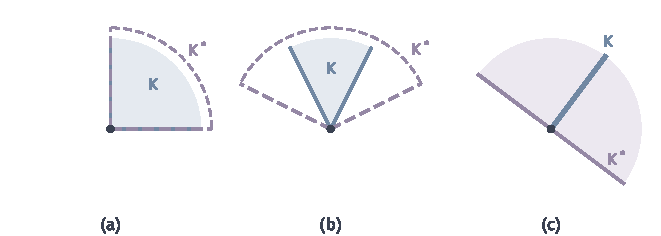
\includegraphics[width=112mm]{figures/05-optimization/06-constrained-optimization/matplotlib/cone-dual-cones/figure.pdf}
  \caption{平面上的锥（蓝色）与对偶锥（紫色）。(a)第一象限的对偶锥是它自身，紫色虚线与蓝色边界重合。(b)窄锥$\{(u,t):\lvert u\rvert\leq t/2\}$的对偶锥是宽锥$\{(v,w):\lvert v\rvert\leq2w\}$。(c)一条射线的对偶锥是一个闭半平面。各锥只画出原点附近的一部分。}
  \label{fig:cone-dual-cones}
\end{BookInlineFigure}

(b)可以手算。设$\bm{K}=\{(u,t):\lvert u\rvert\leq t/2\}$，对$(v,w)$要求$vu+wt\geq0$对所有$\bm{K}$中的点成立。固定$t\geq0$，左端在$u=\pm t/2$中使$vu$为负的那一端最小，最小值是
\[
 -\lvert v\rvert\frac{t}{2}+wt=t\Bigl(w-\frac{\lvert v\rvert}{2}\Bigr).
\]
它对所有$t\geq0$非负，当且仅当$\lvert v\rvert\leq2w$。$\bm{K}$越窄，需要照顾的方向越少，$\bm{K}^*$就越宽。

\paragraph{下界与证书}
第~\ref{chap:duality}章的做法是：把约束乘上乘子加进目标，再对$\bm{x}$取下确界，得到最优值的下界。这里用同样的计算，只是把“非负乘子”换成“对偶锥中的乘子”。

取$\bm{y}\in\mathbb{R}^p$和$\bm{s}\in\bm{K}^*$，构造
\[
 \mathcal{L}(\bm{x},\bm{y},\bm{s})=\bm{c}^\top\bm{x}+\bm{y}^\top(\bm{b}-\bm{A}\bm{x})-\bm{s}^\top(\bm{E}\bm{x}+\bm{g}).
\]
可行的$\bm{x}$满足$\bm{b}-\bm{A}\bm{x}=\bm{0}$，且$\bm{s}^\top(\bm{E}\bm{x}+\bm{g})\geq0$，所以$\mathcal{L}\leq\bm{c}^\top\bm{x}$。

$\mathcal{L}$对$\bm{x}$是仿射的，$\bm{x}$的系数必须为零，下确界才不是$-\infty$。这个条件是$\bm{A}^\top\bm{y}+\bm{E}^\top\bm{s}=\bm{c}$，此时下确界等于$\bm{b}^\top\bm{y}-\bm{g}^\top\bm{s}$。于是得到\term{锥对偶问题}（conic dual problem）
\begin{equation}
 \max_{\bm{y},\bm{s}}\ \bm{b}^\top\bm{y}-\bm{g}^\top\bm{s}\quad\text{s.t.}\quad\bm{A}^\top\bm{y}+\bm{E}^\top\bm{s}=\bm{c},\quad\bm{s}\in\bm{K}^*.
 \label{eq:cone-conic-dual}
\end{equation}

\begin{theorem}[锥规划的弱对偶]
\label{thm:cone-weak-duality}
设$\bm{x}$是问题~\eqref{eq:cone-conic}的可行点，$(\bm{y},\bm{s})$是问题~\eqref{eq:cone-conic-dual}的可行点，则
\begin{equation}
 \bm{c}^\top\bm{x}-(\bm{b}^\top\bm{y}-\bm{g}^\top\bm{s})=\bm{s}^\top(\bm{E}\bm{x}+\bm{g})\geq0.
 \label{eq:cone-conic-gap}
\end{equation}
\end{theorem}

\begin{proof}
把$\bm{c}=\bm{A}^\top\bm{y}+\bm{E}^\top\bm{s}$代入$\bm{c}^\top\bm{x}$，并用$\bm{A}\bm{x}=\bm{b}$，得到
\[
 \bm{c}^\top\bm{x}=\bm{y}^\top\bm{b}+\bm{s}^\top\bm{E}\bm{x}.
\]
两边减去$\bm{b}^\top\bm{y}-\bm{g}^\top\bm{s}$，右端成为$\bm{s}^\top(\bm{E}\bm{x}+\bm{g})$。由$\bm{s}\in\bm{K}^*$和$\bm{E}\bm{x}+\bm{g}\in\bm{K}$，它非负。
\end{proof}

式~\eqref{eq:cone-conic-gap}的用法是：手里有一个原始可行点和一个对偶可行点，最优值就被夹在两个目标值之间。若两个值相等，两个点同时最优。这个判断只用到可行性和内积，不需要知道它们是怎么算出来的。

对线性规划，$\bm{K}^*=\mathbb{R}^n_+$，问题~\eqref{eq:cone-conic-dual}就是第~\ref{chap:linear-programming}章的对偶问题，式~\eqref{eq:cone-conic-gap}就是$\bm{s}^\top\bm{x}\geq0$。

\subsection{二阶锥规划}
\label{sec:cone-socp}

“到某点的距离不超过某个值”是最常见的弯曲约束。这一小节要把它写进锥规划，并弄清右端的符号在其中起什么作用。

\paragraph{二阶锥}
距离上限的形状是一个圆盘。把半径$t$也当作变量，圆盘就随高度放大，叠起来成为一个圆锥。

\begin{definition}[二阶锥规划]
\label{def:cone-socp}
集合
\begin{equation}
 \bm{K}_{\mathrm{so}}^{k+1}=\{(\bm{u},t)\in\mathbb{R}^k\times\mathbb{R}:\lVert\bm{u}\rVert_2\leq t\}
 \label{eq:cone-soc}
\end{equation}
称为\term{二阶锥}（second-order cone）。问题
\begin{equation}
 \begin{aligned}
 \min_{\bm{x}}\quad&\bm{q}^\top\bm{x}\\
 \text{s.t.}\quad&\lVert\bm{A}_i\bm{x}+\bm{b}_i\rVert_2\leq\bm{c}_i^\top\bm{x}+d_i,\quad i=1,\ldots,m,\\
 &\bm{A}\bm{x}=\bm{b}
 \end{aligned}
 \label{eq:cone-socp}
\end{equation}
称为\term{二阶锥规划}（second-order cone program，SOCP）。这里$\bm{A}_i\in\mathbb{R}^{k_i\times n}$，$\bm{b}_i\in\mathbb{R}^{k_i}$，$\bm{c}_i\in\mathbb{R}^n$，$d_i\in\mathbb{R}$。
\end{definition}

第$i$条约束说的正是
\[
 (\bm{A}_i\bm{x}+\bm{b}_i,\ \bm{c}_i^\top\bm{x}+d_i)\in\bm{K}_{\mathrm{so}}^{k_i+1}.
\]

这个集合确实是闭凸锥。放缩时范数按倍数变化，$\theta\geq0$时仍有$\lVert\theta\bm{u}\rVert_2\leq\theta t$；相加时由三角不等式，
\[
 \lVert\bm{u}_1+\bm{u}_2\rVert_2\leq\lVert\bm{u}_1\rVert_2+\lVert\bm{u}_2\rVert_2\leq t_1+t_2.
\]
放缩和相加封闭，合起来就是凸。闭性来自范数连续。

图~\ref{fig:cone-soc-3d}画出$k=2$时的二阶锥，高度为$t$的水平截面是半径为$t$的圆盘。

\begin{BookInlineFigure}
  \centering
  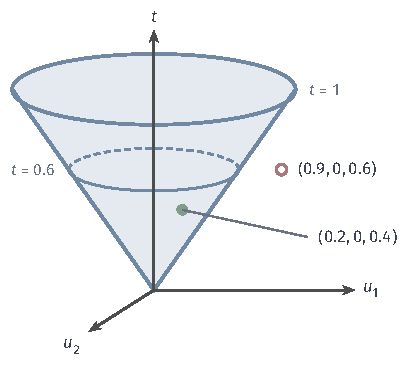
\includegraphics[width=66mm]{figures/05-optimization/06-constrained-optimization/tikz/cone-soc-3d/figure.pdf}
  \caption{$\mathbb{R}^3$中的二阶锥$\sqrt{u_1^2+u_2^2}\leq t$，画出$0\leq t\leq1$的部分。绿点$(0.2,0,0.4)$满足$0.2\leq0.4$，在锥内。红色空心点$(0.9,0,0.6)$不满足$0.9\leq0.6$，在锥外。}
  \label{fig:cone-soc-3d}
\end{BookInlineFigure}

\paragraph{右端非负也是条件的一部分}
约束的左端是范数，总是非负的，所以满足约束就迫使$\bm{c}_i^\top\bm{x}+d_i\geq0$。这个隐含的符号条件不可丢弃。

有人会想两边平方，把约束写成$\lVert\bm{u}\rVert_2^2\leq t^2$。这一步改变了集合。正确的等价关系是
\begin{equation}
 \lVert\bm{u}\rVert_2\leq t\quad\Longleftrightarrow\quad t\geq0\text{ 且 }\lVert\bm{u}\rVert_2^2\leq t^2.
 \label{eq:cone-soc-square}
\end{equation}
去掉$t\geq0$后，$(u,t)=(1,-2)$满足$1\leq4$，却不满足$1\leq-2$。

图~\ref{fig:cone-soc-square}对比了两个集合。平方之后得到的是上下两片，这个集合甚至不凸。

\begin{BookInlineFigure}
  \centering
  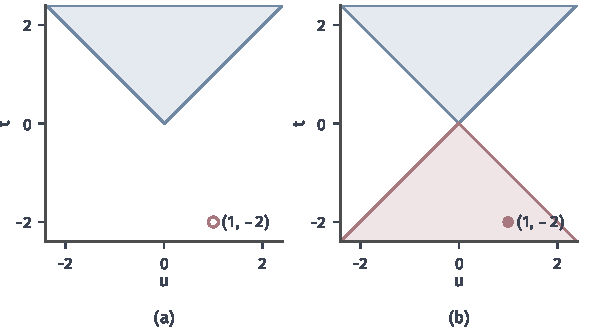
\includegraphics[width=100mm]{figures/05-optimization/06-constrained-optimization/matplotlib/cone-soc-square/figure.pdf}
  \caption{平方丢失符号信息。(a)二阶锥$\lvert u\rvert\leq t$，点$(1,-2)$不在其中。(b)$u^2\leq t^2$的解集多出了红色的下半部分，点$(1,-2)$落在其中，集合不再是凸集。}
  \label{fig:cone-soc-square}
\end{BookInlineFigure}

\paragraph{距离上限的交集}
下面用一个能手算的例子看这类可行集。在两个圆盘的公共部分里求最低的点：
\begin{equation}
 \min_{\bm{x}\in\mathbb{R}^2}\ x_2\quad\text{s.t.}\quad\lVert\bm{x}-\bm{a}_1\rVert_2\leq5,\quad\lVert\bm{x}-\bm{a}_2\rVert_2\leq5,
 \label{eq:cone-lens}
\end{equation}
其中$\bm{a}_1=(0,0)$，$\bm{a}_2=(6,0)$。对照式~\eqref{eq:cone-socp}，$\bm{q}=(0,1)$，$\bm{A}_i=\bm{I}$，$\bm{b}_i=-\bm{a}_i$，$\bm{c}_i=\bm{0}$，$d_i=5$。

每条约束是一个圆盘，二者的交仍是凸集，形状像一枚透镜，如图~\ref{fig:cone-soc-lens}所示。它的边界是弯的，所以不是多面体，线性规划和二次规划的可行集都表达不了。

\begin{BookInlineFigure}
  \centering
  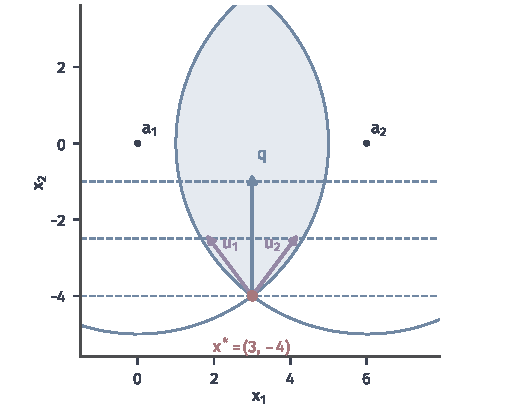
\includegraphics[width=88mm]{figures/05-optimization/06-constrained-optimization/matplotlib/cone-soc-lens/figure.pdf}
  \caption{两条距离约束的交集。浅蓝透镜是可行集，蓝色虚线是目标$x_2$的等值线，红点是解$(3,-4)$。紫色箭头是第~\ref{sec:cone-duality-certificates}小节算出的乘子分量$\bm{u}_1,\bm{u}_2$，蓝色箭头是目标系数$\bm{q}=\bm{u}_1+\bm{u}_2$，三者同乘$3.2$后画出。}
  \label{fig:cone-soc-lens}
\end{BookInlineFigure}

透镜的最低点是两个圆的交点。把两个圆的方程相减，
\[
 x_1^2+x_2^2-(x_1-6)^2-x_2^2=0,
\]
化简得$x_1=3$。代回第一个圆，得到$x_2=\pm4$。所以候选解是$(3,-4)$，目标值$-4$。它确实最优，稍后用对偶解来证明。

\paragraph{右端含变量}
约束右端也可以依赖决策变量。设要找一个位置$\bm{x}$，使它到三个站点的最大距离最小。引入变量$t$表示这个最大距离，问题写成
\begin{equation}
 \min_{\bm{x},t}\ t\quad\text{s.t.}\quad\lVert\bm{x}-\bm{p}_i\rVert_2\leq t,\quad i=1,2,3.
 \label{eq:cone-enclosing}
\end{equation}
这里决策变量是$(\bm{x},t)\in\mathbb{R}^3$，每条约束的右端$\bm{c}_i^\top(\bm{x},t)+d_i$就是$t$。在$(\bm{x},t)$空间里，每条约束是一个顶点在$(\bm{p}_i,0)$的圆锥，可行集是三个圆锥的交。

取$\bm{p}_1=(0,0)$，$\bm{p}_2=(6,0)$，$\bm{p}_3=(3,9)$。点$\bm{x}^\star=(3,4)$到三个站点的距离都是$5$，图~\ref{fig:cone-soc-enclosing}(a)是相应的覆盖圆。

\begin{BookInlineFigure}
  \centering
  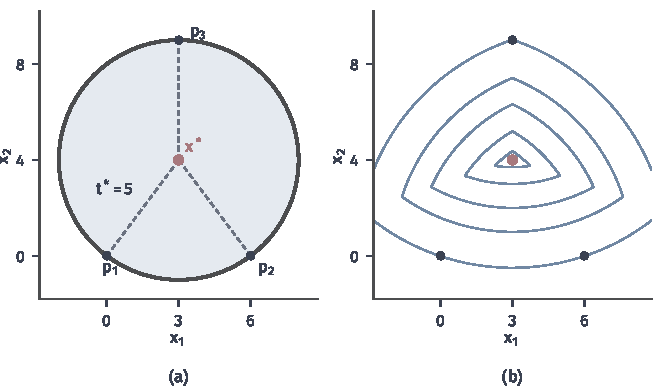
\includegraphics[width=112mm]{figures/05-optimization/06-constrained-optimization/matplotlib/cone-soc-enclosing/figure.pdf}
  \caption{最小化到三个站点的最大距离。(a)红点到三个站点的距离都等于$t^\star=5$，深灰圆是覆盖三点的最小圆。(b)蓝线是函数$\max_i\lVert\bm{x}-\bm{p}_i\rVert_2$的等高线，三段圆弧在折角处相接，目标不可微，而写成式~\eqref{eq:cone-enclosing}后目标和约束都很规则。}
  \label{fig:cone-soc-enclosing}
\end{BookInlineFigure}

下面验证$\bm{x}^\star$最优。三个站点相对$\bm{x}^\star$的位置是$(-3,-4)$、$(3,-4)$、$(0,5)$，用正权重$5,5,8$加权，和为零：
\[
 5\begin{bmatrix}-3\\-4\end{bmatrix}+5\begin{bmatrix}3\\-4\end{bmatrix}+8\begin{bmatrix}0\\5\end{bmatrix}=\bm{0}.
\]
所以对任何位移$\bm{d}\neq\bm{0}$，三个数$\bm{d}^\top(\bm{p}_i-\bm{x}^\star)$不可能全部非负且不全为零；又因三个向量张成平面，它们也不会全为零。因此总有某个$i$使$\bm{d}^\top(\bm{p}_i-\bm{x}^\star)<0$。

对这个$i$，位移后的距离满足
\[
 \lVert\bm{x}^\star+\bm{d}-\bm{p}_i\rVert_2^2=25+\lVert\bm{d}\rVert_2^2-2\bm{d}^\top(\bm{p}_i-\bm{x}^\star)>25.
\]
最大距离严格变大，所以$\bm{x}^\star$是唯一的最优位置，$t^\star=5$。

\subsection{半正定规划}
\label{sec:cone-sdp}

有些量天然是矩阵，而且必须像协方差矩阵那样半正定。这一小节回答：矩阵半正定的约束怎样放进锥规划，它能表达哪些条件，又怎样用特征值检验？

\paragraph{矩阵作变量}
记$\mathcal{S}^n$为$n\times n$实对称矩阵组成的线性空间。在其上使用\term{迹内积}（trace inner product）
\begin{equation}
 \langle\bm{X},\bm{Y}\rangle=\operatorname{tr}(\bm{X}\bm{Y})=\sum_{i,j}X_{i,j}Y_{i,j}.
 \label{eq:cone-trace-inner}
\end{equation}
把矩阵按元素排成长向量，这就是普通的欧氏内积。

半正定矩阵的集合记为$\mathcal{S}^n_+$。$\bm{X}\in\mathcal{S}^n_+$的定义是对所有$\bm{v}$有$\bm{v}^\top\bm{X}\bm{v}\geq0$，等价于全部特征值非负，这个等价关系可参考\BookChapterRef{chap:eigen-spectral-decomposition}{卷二第6章“谱分解”}。

$\mathcal{S}^n_+$是闭凸锥。对固定的$\bm{v}$，$\bm{v}^\top\bm{X}\bm{v}\geq0$是$\bm{X}$的一个线性不等式，定义的是过原点的闭半空间。$\mathcal{S}^n_+$是无穷多个这样的闭半空间的交，所以它闭、凸，且对非负放缩封闭。

\begin{definition}[半正定规划]
\label{def:cone-sdp}
给定$\bm{W},\bm{A}_1,\ldots,\bm{A}_m\in\mathcal{S}^n$和$\bm{b}\in\mathbb{R}^m$，问题
\begin{equation}
 \begin{aligned}
 \min_{\bm{X}\in\mathcal{S}^n}\quad&\langle\bm{W},\bm{X}\rangle\\
 \text{s.t.}\quad&\langle\bm{A}_i,\bm{X}\rangle=b_i,\quad i=1,\ldots,m,\\
 &\bm{X}\succeq\bm{0}
 \end{aligned}
 \label{eq:cone-sdp}
\end{equation}
称为\term{半正定规划}（semidefinite program，SDP）。$\bm{X}\succeq\bm{0}$表示$\bm{X}\in\mathcal{S}^n_+$。
\end{definition}

\paragraph{半正定不是逐元素非负}
“$\bm{X}\succeq\bm{0}$”和“$\bm{X}$的元素非负”容易混淆，其实二者互不包含。$\begin{bmatrix}1&2\\2&1\end{bmatrix}$元素全正，特征值却有$-1$。$\begin{bmatrix}1&-1\\-1&1\end{bmatrix}$有负元素，特征值是$0$和$2$，半正定。

为了看清这个差别，取迹为$1$的$2\times2$对称矩阵
\[
 \bm{X}=\begin{bmatrix}a&b\\b&1-a\end{bmatrix}.
\]
$2\times2$矩阵半正定，当且仅当两个对角元和行列式都非负。这里就是$a(1-a)-b^2\geq0$，配方得到
\[
 \Bigl(a-\frac12\Bigr)^2+b^2\leq\frac14.
\]
半正定的矩阵组成一个圆盘，而逐元素非负的要求是一条竖带的上半部分，见图~\ref{fig:cone-sdp-disk}。

\begin{BookInlineFigure}
  \centering
  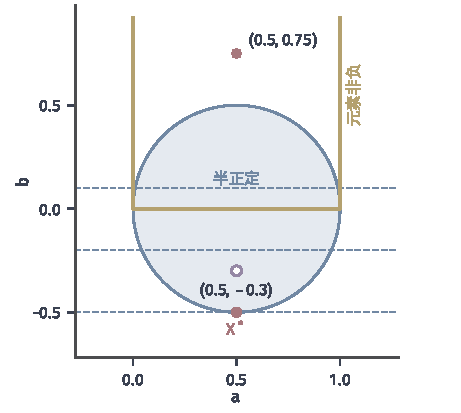
\includegraphics[width=78mm]{figures/05-optimization/06-constrained-optimization/matplotlib/cone-sdp-disk/figure.pdf}
  \caption{迹为$1$的$2\times2$对称矩阵$\begin{bmatrix}a&b\\b&1-a\end{bmatrix}$。浅蓝圆盘是半正定矩阵，黄线围住的是逐元素非负的矩阵。红色方块$(0.5,0.75)$元素非负但不半正定，紫色空心点$(0.5,-0.3)$半正定但有负元素。蓝色虚线是目标$2+2b$的等值线，红点是最优矩阵$\bm{X}^\star$。}
  \label{fig:cone-sdp-disk}
\end{BookInlineFigure}

可行集的边界是圆，所以半正定规划的最优解一般不在有限个候选的“顶点”上。在这个切片上取$\bm{W}=\begin{bmatrix}2&1\\1&2\end{bmatrix}$，最小化$\langle\bm{W},\bm{X}\rangle$，约束是$\operatorname{tr}\bm{X}=1$、$\bm{X}\succeq\bm{0}$。按式~\eqref{eq:cone-trace-inner}计算，
\[
 \langle\bm{W},\bm{X}\rangle=2a+2b+2(1-a)=2+2b.
\]
目标只依赖$b$，最小值在圆盘最低点$(a,b)=(1/2,-1/2)$取得，最优值是$1$，这正是$\bm{W}$的最小特征值。最优矩阵是
\[
 \bm{X}^\star=\frac12\begin{bmatrix}1&-1\\-1&1\end{bmatrix}.
\]

\paragraph{线性矩阵不等式}
实际问题常把变量放在矩阵的元素上，得到下面的约束：
\begin{equation}
 \bm{F}_0+x_1\bm{F}_1+\cdots+x_n\bm{F}_n\succeq\bm{0},
 \label{eq:cone-lmi}
\end{equation}
其中$\bm{F}_j\in\mathcal{S}^k$。这称为\term{线性矩阵不等式}（linear matrix inequality，LMI）。它正是式~\eqref{eq:cone-conic}中取$\bm{K}=\mathcal{S}^k_+$的情形，$\bm{E}\bm{x}+\bm{g}$是$\bm{x}$的仿射函数，取值为矩阵。

一条线性矩阵不等式可以表达弯曲的集合。例如
\[
 \bm{F}(\bm{x})=\begin{bmatrix}1+x_1&x_2\\x_2&1-x_1\end{bmatrix}
\]
的特征值是$1\pm\lVert\bm{x}\rVert_2$，所以$\bm{F}(\bm{x})\succeq\bm{0}$恰好是单位圆盘。

检验一个点是否可行，只需算特征值。取$\bm{x}=(0.6,0.6)$，特征值约为$0.152$和$1.849$，都为正，可行。取$\bm{x}=(0.8,0.8)$，最小特征值约为$-0.131$，不可行。图~\ref{fig:cone-sdp-lmi}(a)画出这两个点。

\begin{BookInlineFigure}
  \centering
  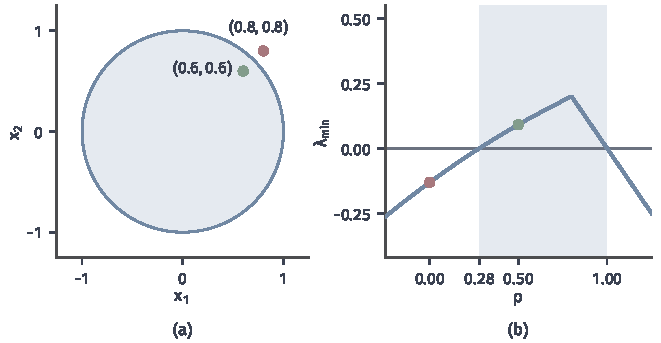
\includegraphics[width=112mm]{figures/05-optimization/06-constrained-optimization/matplotlib/cone-sdp-lmi/figure.pdf}
  \caption{用特征值检验线性矩阵不等式。(a)$\bm{F}(\bm{x})\succeq\bm{0}$的解集是单位圆盘，绿点可行，红点不可行。(b)相关矩阵~\eqref{eq:cone-corr-matrix}的最小特征值随$\rho$的变化，浅蓝区间$[0.28,1]$是使矩阵半正定的$\rho$。绿点$\rho=0.5$可行，红点$\rho=0$不可行。}
  \label{fig:cone-sdp-lmi}
\end{BookInlineFigure}

\paragraph{协方差约束}
线性矩阵不等式的一个典型来源是协方差矩阵必须半正定。设三个量两两的相关系数中，已知$\rho_{1,2}=\rho_{2,3}=0.8$，问$\rho_{1,3}=\rho$能取哪些值。相关矩阵是
\begin{equation}
 \bm{R}(\rho)=\begin{bmatrix}1&0.8&\rho\\0.8&1&0.8\\\rho&0.8&1\end{bmatrix}.
 \label{eq:cone-corr-matrix}
\end{equation}
协方差矩阵半正定这一事实的来源可参考\BookChapterRef{chap:random-vectors}{卷七第2章“随机向量与联合分布”}。这里只用到结论：$\bm{R}(\rho)$不半正定，就不存在这样的三个随机变量。

取$\rho=0$，矩阵的元素都非负，特征值却约为$-0.131$、$1$和$2.131$。所以$\rho=0$不可能，1与2强相关、2与3强相关时，1与3不能不相关。

取$\rho=0.5$，特征值约为$0.091$、$0.5$和$2.409$，可行。一般地，
\[
 \det\bm{R}(\rho)=-(\rho-1)(\rho-0.28),
\]
结合$\lvert\rho\rvert\leq1$可知可行范围是$0.28\leq\rho\leq1$，与图~\ref{fig:cone-sdp-lmi}(b)一致。

\paragraph{谱上界}
另一类重要的表达能力是控制特征值。设对称矩阵$\bm{B}(\bm{x})$仿射地依赖$\bm{x}$。对谱分解后的每个特征值看，$\lambda_{\max}(\bm{B}(\bm{x}))\leq t$等价于$t\bm{I}-\bm{B}(\bm{x})$的特征值全部非负，即
\begin{equation}
 \lambda_{\max}(\bm{B}(\bm{x}))\leq t\quad\Longleftrightarrow\quad t\bm{I}-\bm{B}(\bm{x})\succeq\bm{0}.
 \label{eq:cone-spectral-bound}
\end{equation}
所以最小化最大特征值可以写成半正定规划：在式~\eqref{eq:cone-spectral-bound}的约束下最小化$t$。

看一个具体的例子：
\[
 \bm{B}(x)=\begin{bmatrix}1+x&1\\1&3-x\end{bmatrix}.
\]
它的特征值是$2\pm\sqrt{(1-x)^2+1}$，所以$\lambda_{\max}$在$x=1$取最小值$3$。这是一个光滑例子，但$\lambda_{\max}$在特征值重合处通常不可微，而写成式~\eqref{eq:cone-spectral-bound}后，非光滑性消失在锥约束里。图~\ref{fig:cone-sdp-spectral}画出这个例子，图中的紫线下一小节解释。

\begin{BookInlineFigure}
  \centering
  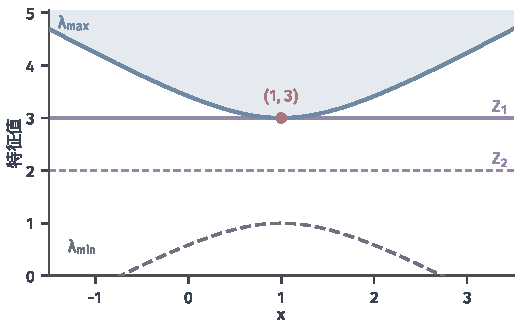
\includegraphics[width=88mm]{figures/05-optimization/06-constrained-optimization/matplotlib/cone-sdp-spectral/figure.pdf}
  \caption{$\bm{B}(x)$的两个特征值。浅蓝区域是$\lambda_{\max}(\bm{B}(x))\leq t$的$(x,t)$，红点是最优解。紫色实线$Z_1$是由$\bm{Z}_1=\frac12\begin{bmatrix}1&1\\1&1\end{bmatrix}$给出的下界$3$，紫色虚线$Z_2$是由$\bm{Z}_2=\frac12\bm{I}$给出的下界$2$。}
  \label{fig:cone-sdp-spectral}
\end{BookInlineFigure}

\subsection{锥对偶与证书}
\label{sec:cone-duality-certificates}

对偶问题~\eqref{eq:cone-conic-dual}要用到$\bm{K}^*$。这一小节算出三种常用锥的对偶锥，写出对应的对偶问题，再说明弱对偶可以放心使用，而强对偶需要额外的条件。

\paragraph{自对偶性}
下面的定理说，这三种锥的乘子就在原来的锥里取。

\begin{theorem}[三种常用锥的自对偶性]
\label{thm:cone-self-dual}
$\mathbb{R}^n_+$、$\bm{K}_{\mathrm{so}}^{k+1}$和$\mathcal{S}^n_+$的对偶锥都是它们自身。其中$\mathcal{S}^n_+$的内积取迹内积。
\end{theorem}

\begin{proof}
\emph{非负象限。}若$\bm{s}\geq\bm{0}$，对$\bm{x}\geq\bm{0}$有$\bm{s}^\top\bm{x}\geq0$。反过来，若$s_i<0$，取$\bm{x}=\bm{e}_i$得$\bm{s}^\top\bm{x}<0$。

\emph{二阶锥。}设$(\bm{v},w)$、$(\bm{u},t)$都在二阶锥中。由Cauchy--Schwarz不等式，
\[
 \bm{v}^\top\bm{u}+wt\geq-\lVert\bm{v}\rVert_2\lVert\bm{u}\rVert_2+wt\geq-wt+wt=0.
\]
所以二阶锥包含于它的对偶锥。

反过来，设$(\bm{v},w)$在对偶锥中。取$(\bm{u},t)=(\bm{0},1)$，得$w\geq0$。若$\bm{v}\neq\bm{0}$，取$\bm{u}=-\bm{v}/\lVert\bm{v}\rVert_2$、$t=1$，得到$-\lVert\bm{v}\rVert_2+w\geq0$。这两种情形都给出$\lVert\bm{v}\rVert_2\leq w$。

\emph{半正定锥。}设$\bm{X},\bm{S}\succeq\bm{0}$，由谱分解取半正定平方根，
\[
 \langle\bm{S},\bm{X}\rangle=\operatorname{tr}(\bm{S}^{1/2}\bm{X}\bm{S}^{1/2})\geq0,
\]
因为$\bm{S}^{1/2}\bm{X}\bm{S}^{1/2}$半正定，迹就是非负特征值之和。

反过来，设$\bm{S}$在对偶锥中。对任意$\bm{v}$，取$\bm{X}=\bm{v}\bm{v}^\top\succeq\bm{0}$，得到
\[
 \langle\bm{S},\bm{v}\bm{v}^\top\rangle=\bm{v}^\top\bm{S}\bm{v}\geq0,
\]
所以$\bm{S}\succeq\bm{0}$。
\end{proof}

半正定锥的乘子是半正定矩阵，不是元素非负的矩阵；二阶锥的乘子也有分量可以为负。线性规划里“乘子非负”这句话，推广之后是“乘子属于对偶锥”。

\paragraph{写出对偶问题}
把定理~\ref{thm:cone-self-dual}代入式~\eqref{eq:cone-conic-dual}。对二阶锥规划~\eqref{eq:cone-socp}，每条约束对应乘子$(\bm{u}_i,\tau_i)$，等式的乘子记作$\bm{y}$。按定义逐项写出，对偶问题是
\begin{equation}
 \begin{aligned}
 \max\quad&\bm{b}^\top\bm{y}-\sum_{i=1}^m(\bm{b}_i^\top\bm{u}_i+d_i\tau_i)\\
 \text{s.t.}\quad&\bm{A}^\top\bm{y}+\sum_{i=1}^m(\bm{A}_i^\top\bm{u}_i+\tau_i\bm{c}_i)=\bm{q},\\
 &\lVert\bm{u}_i\rVert_2\leq\tau_i,\quad i=1,\ldots,m.
 \end{aligned}
 \label{eq:cone-socp-dual}
\end{equation}

半正定规划~\eqref{eq:cone-sdp}中$\bm{X}$本身属于锥，相当于$\bm{E}$是恒等映射、$\bm{g}=\bm{0}$，对偶问题是
\begin{equation}
 \max_{\bm{y},\bm{S}}\ \bm{b}^\top\bm{y}\quad\text{s.t.}\quad\sum_{i=1}^my_i\bm{A}_i+\bm{S}=\bm{W},\quad\bm{S}\succeq\bm{0}.
 \label{eq:cone-sdp-dual}
\end{equation}
相应的间隙公式是
\begin{equation}
 \langle\bm{W},\bm{X}\rangle-\bm{b}^\top\bm{y}=\langle\bm{S},\bm{X}\rangle.
 \label{eq:cone-sdp-gap}
\end{equation}

\begin{example}[透镜问题的对偶证书]
\label{ex:cone-lens-dual}
对问题~\eqref{eq:cone-lens}，式~\eqref{eq:cone-socp-dual}成为：在$\bm{u}_1+\bm{u}_2=\bm{q}$、$\lVert\bm{u}_i\rVert_2\leq\tau_i$下最大化
\[
 \bm{a}_1^\top\bm{u}_1+\bm{a}_2^\top\bm{u}_2-5\tau_1-5\tau_2.
\]
先任取一个可行的乘子，看它给出什么下界。取$\bm{u}_1=\bm{u}_2=(0,1/2)$，$\tau_1=\tau_2=1/2$，对偶目标是$-5$。所以无论可行点是什么，$x_2\geq-5$，这个下界对，但不紧。

要使间隙为零，由式~\eqref{eq:cone-conic-gap}，每条约束的$(\bm{u}_i,\tau_i)$必须与$(\bm{x}^\star-\bm{a}_i,5)$内积为零。两个向量都在二阶锥的边界上时，这要求$\bm{u}_i$与$\bm{x}^\star-\bm{a}_i$反向，且$\lVert\bm{u}_i\rVert_2=\tau_i$。

在$\bm{x}^\star=(3,-4)$处，这给出
\[
 \bm{u}_1=\tau_1\begin{bmatrix}-3/5\\4/5\end{bmatrix},\qquad
 \bm{u}_2=\tau_2\begin{bmatrix}3/5\\4/5\end{bmatrix}.
\]
再由$\bm{u}_1+\bm{u}_2=(0,1)$，解得
\[
 \tau_1=\tau_2=\frac58,\qquad
 \bm{u}_1=\begin{bmatrix}-3/8\\1/2\end{bmatrix},\qquad
 \bm{u}_2=\begin{bmatrix}3/8\\1/2\end{bmatrix}.
\]
对偶目标是
\[
 0+\frac{18}{8}-\frac{25}{8}-\frac{25}{8}=-4.
\]
它等于原始目标值，所以$(3,-4)$最优，这对乘子也最优。图~\ref{fig:cone-soc-lens}中的紫色箭头画的就是$\bm{u}_1,\bm{u}_2$，二者之和是目标的梯度。
\end{example}

\begin{example}[谱上界的对偶证书]
\label{ex:cone-spectral-dual}
对$\min t$、$t\bm{I}-\bm{B}(x)\succeq\bm{0}$，取乘子$\bm{Z}\succeq\bm{0}$。不必套公式，直接从谱上界出发：任何$\operatorname{tr}\bm{Z}=1$的$\bm{Z}\succeq\bm{0}$都满足
\[
 \lambda_{\max}(\bm{B}(x))\geq\langle\bm{Z},\bm{B}(x)\rangle,
\]
因为$\lambda_{\max}\bm{I}-\bm{B}(x)\succeq\bm{0}$与$\bm{Z}$的迹内积非负。

若再选$\bm{Z}$使右端不含$x$，就得到一个对所有$x$成立的常数下界。$\bm{B}(x)$中$x$的系数是$\operatorname{diag}(1,-1)$，所以要求$Z_{1,1}=Z_{2,2}$，再由迹为$1$得$Z_{1,1}=Z_{2,2}=1/2$。取$Z_{1,2}=1/2$，得到
\[
 \bm{Z}_1=\frac12\begin{bmatrix}1&1\\1&1\end{bmatrix},\qquad
 \langle\bm{Z}_1,\bm{B}(x)\rangle=\frac12(1+x+2+3-x)=3.
\]
变量$x$消掉了，于是$\lambda_{\max}(\bm{B}(x))\geq3$对所有$x$成立。$x=1$时取等，这就是最优性的证明，即图~\ref{fig:cone-sdp-spectral}的紫色实线。

取$Z_{1,2}=0$，同样的计算给出常数$2$，下界正确但不紧，是图中的紫色虚线。
\end{example}

\paragraph{矩阵互补}
式~\eqref{eq:cone-conic-gap}说明，零间隙等价于$\bm{s}^\top(\bm{E}\bm{x}+\bm{g})=0$，这是互补松弛的锥形式。半正定时，这个条件比一个数等于零更强。

设$\bm{X},\bm{S}\succeq\bm{0}$且$\langle\bm{S},\bm{X}\rangle=0$，则
\[
 \operatorname{tr}(\bm{S}^{1/2}\bm{X}\bm{S}^{1/2})=\lVert\bm{X}^{1/2}\bm{S}^{1/2}\rVert_{\mathrm{F}}^2=0.
\]
所以$\bm{X}^{1/2}\bm{S}^{1/2}=\bm{0}$，再两边分别乘$\bm{X}^{1/2}$和$\bm{S}^{1/2}$，得到
\begin{equation}
 \bm{X}\bm{S}=\bm{0}.
 \label{eq:cone-matrix-complementarity}
\end{equation}
二者的列空间互相正交，秩之和不超过$n$。

以迹为$1$的例子验证。对偶问题是$\max y$、$\bm{S}=\bm{W}-y\bm{I}\succeq\bm{0}$，最优值在$y=\lambda_{\min}(\bm{W})=1$取得。这时
\[
 \bm{S}=\begin{bmatrix}1&1\\1&1\end{bmatrix},\qquad
 \bm{X}^\star\bm{S}=\frac12\begin{bmatrix}1&-1\\-1&1\end{bmatrix}\begin{bmatrix}1&1\\1&1\end{bmatrix}=\bm{0}.
\]

\paragraph{强对偶需要条件}
弱对偶无条件成立，证书就是这么来的。但两个目标值是否一定能碰到一起？线性规划中，只要原始和对偶都可行，最优值就相等且都能取到。这一结论不能原样推广。

类似第~\ref{chap:duality}章的Slater条件，锥规划也有严格可行性的条件。若存在满足$\bm{A}\bm{x}=\bm{b}$且$\bm{E}\bm{x}+\bm{g}\in\operatorname{int}\bm{K}$的点，并且原始最优值有限，则对偶问题取得最优解，且间隙为零。把原始和对偶的角色对调，结论同样成立。证明用凸集分离定理，与Slater条件的论证相同，只是把标量不等式换成锥成员条件，读者可查阅凸优化教材\scite{math-boyd2004convex}。

下面两个例子说明缺少这一条件时会出什么问题。

\begin{example}[最优值取不到]
\label{ex:cone-non-attain}
考虑
\[
 \min_{\bm{x}}\ x_1\quad\text{s.t.}\quad\begin{bmatrix}x_1&1\\1&x_2\end{bmatrix}\succeq\bm{0}.
\]
约束等价于$x_1,x_2>0$且$x_1x_2\geq1$，可行集是双曲线上方的区域，如图~\ref{fig:cone-sdp-gaps}(a)所示。取$x_1=1/k$、$x_2=k$，目标趋于$0$，但$x_1=0$不可行，最优值$0$取不到。

把式~\eqref{eq:cone-conic-dual}写出来：$\bm{Z}\succeq\bm{0}$，$Z_{1,1}=1$，$Z_{2,2}=0$，目标是$-2Z_{1,2}$。半正定和$Z_{2,2}=0$迫使$Z_{1,2}=0$，对偶唯一的可行值是$0$，它取到了。

这里原始严格可行（取$x_1=x_2=2$），所以对偶取得最优且间隙为零，符合上面的结论。对偶没有严格可行点，所以原始不保证取得最优解。
\end{example}

\begin{example}[正的对偶间隙]
\label{ex:cone-positive-gap}
考虑
\[
 \min_{\bm{x}}\ x_1\quad\text{s.t.}\quad\begin{bmatrix}0&x_1&0\\x_1&x_2&0\\0&0&x_1+1\end{bmatrix}\succeq\bm{0}.
\]
半正定矩阵的对角元为零时，同行同列都为零，所以$x_1=0$，$p^\star=0$。

对偶问题的乘子$\bm{Z}\succeq\bm{0}$要满足两个条件。$x_2$的系数给出$Z_{2,2}=0$，从而$Z_{1,2}=0$。$x_1$的系数给出$2Z_{1,2}+Z_{3,3}=1$，从而$Z_{3,3}=1$。

对偶目标是$-Z_{3,3}=-1$，所以$d^\star=-1$。原始和对偶都可行，也都取到最优值，二者却相差$1$，见图~\ref{fig:cone-sdp-gaps}(b)。原始可行集的矩阵全部奇异，严格可行性不成立。
\end{example}

\begin{BookInlineFigure}
  \centering
  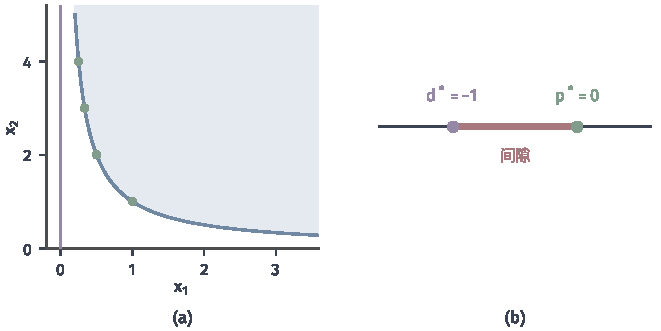
\includegraphics[width=112mm]{figures/05-optimization/06-constrained-optimization/matplotlib/cone-sdp-gaps/figure.pdf}
  \caption{半正定规划强对偶失效的两种方式。(a)浅蓝区域是可行集$x_1x_2\geq1$，绿点$(1/k,k)$的目标趋于紫线$x_1=0$，但永远到不了。(b)原始最优值$0$（绿）与对偶最优值$-1$（紫）之间有正间隙（红）。}
  \label{fig:cone-sdp-gaps}
\end{BookInlineFigure}

这些现象的根源在于，闭凸锥在线性映射下的像不一定闭。非负象限是多面体，多面体的线性像仍是闭集，二阶锥和半正定锥则没有这个保证。表~\ref{tab:cone-duality-compare}归纳了差别。

\begin{BookInlineTable}
  \centering
  \begin{tabular}{lll}
    \toprule
    性质 & 线性规划 & 一般锥规划\\
    \midrule
    弱对偶 & 成立 & 成立\\
    两边可行时间隙为零 & 成立 & 不一定\\
    最优值能取到 & 有限时取到 & 不一定\\
    零间隙的依据 & 无需额外条件 & 严格可行性等条件\\
    \bottomrule
  \end{tabular}
  \caption{线性规划与一般锥规划的对偶性质对比。}
  \label{tab:cone-duality-compare}
\end{BookInlineTable}

所以报告半正定规划的结果时，弱对偶给出的界永远可靠；“间隙为零”这句话则要么由算出的两个可行解直接验证，要么先核对严格可行性。

\section{等价改写}
\label{sec:cone-rewrite}

实际问题很少一开始就长成式~\eqref{eq:cone-qp}或式~\eqref{eq:cone-conic}的样子，常要引入辅助变量才能写进去。这就需要回答：引入辅助变量、换了约束之后，凭什么说问题没有变？

\paragraph{什么叫没有改变问题}
设原问题是在$\bm{C}$上最小化$f(\bm{x})$，改写后的问题是在$\bm{C}'$上最小化$\phi(\bm{x},\bm{z})$，其中$\bm{z}$是辅助变量。要说二者等价，需要两个方向的对应。

\begin{definition}[等价改写]
\label{def:cone-equivalent}
若下面两条都成立，则称改写后的问题是原问题的\term{等价改写}（equivalent reformulation）：
\begin{enumerate}
 \item 对每个$\bm{x}\in\bm{C}$，存在$\bm{z}$使$(\bm{x},\bm{z})\in\bm{C}'$，且$\phi(\bm{x},\bm{z})\leq f(\bm{x})$；
 \item 对每个$(\bm{x},\bm{z})\in\bm{C}'$，都有$\bm{x}\in\bm{C}$，且$f(\bm{x})\leq\phi(\bm{x},\bm{z})$。
\end{enumerate}
\end{definition}

第一条说原问题的每个候选都有替身，而且替身的代价不更高。第二条说消去辅助变量后回到的正是原约束，代价也没有被低估。

\begin{theorem}[等价改写保持最优值与最优解]
\label{thm:cone-equivalent}
在定义~\ref{def:cone-equivalent}的条件下，两个问题的最优值相等。若$(\bm{x}^\star,\bm{z}^\star)$是改写问题的最优解，则$\bm{x}^\star$是原问题的最优解。若$\bm{x}^\star$是原问题的最优解，则它配上第一条中的$\bm{z}$是改写问题的最优解。
\end{theorem}

\begin{proof}
记两个最优值为$p$和$p'$。第一条说明，原问题的每个目标值都不低于改写问题的某个目标值，于是$p'\leq p$。第二条同理给出$p\leq p'$，所以$p=p'$。

设$(\bm{x}^\star,\bm{z}^\star)$最优。第二条给出$\bm{x}^\star\in\bm{C}$，以及
\[
 f(\bm{x}^\star)\leq\phi(\bm{x}^\star,\bm{z}^\star)=p'=p.
\]
所以$\bm{x}^\star$最优。

设$\bm{x}^\star$最优，取第一条中的$\bm{z}$。则$(\bm{x}^\star,\bm{z})$可行，且
\[
 \phi(\bm{x}^\star,\bm{z})\leq f(\bm{x}^\star)=p=p'.
\]
所以它最优。
\end{proof}

定理同时给出了恢复原变量的办法：解改写问题，然后把辅助变量丢掉。对照图~\ref{fig:cone-rewrite-project}(a)，改写后的可行集沿辅助变量方向投影，恰好覆盖原可行集。

\begin{BookInlineFigure}
  \centering
  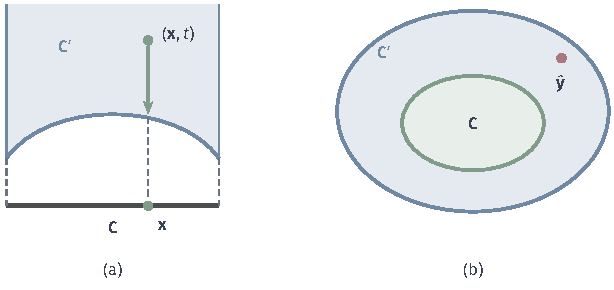
\includegraphics[width=104mm]{figures/05-optimization/06-constrained-optimization/tikz/cone-rewrite-project/figure.pdf}
  \caption{等价改写与松弛的区别。(a)等价改写：点$(\bm{x},t)$沿竖直方向下移不增加代价，投影后回到$\bm{C}$，$\bm{C}'$的投影恰是$\bm{C}$（深灰线段）。(b)松弛：$\bm{C}'$严格包含$\bm{C}$，$\bm{C}'$中可能有红点$\hat{\bm{y}}$这样不对应任何原可行点的元素，所以只保留定义中的第一条。}
  \label{fig:cone-rewrite-project}
\end{BookInlineFigure}

若只有第一条成立，得到的是另一种东西：改写后的问题最优值不超过原问题，但它的解可能不对应任何原可行点。这就是图中的(b)，留到第~\ref{sec:cone-relax}节讨论。

\subsection{上图形式}
\label{sec:cone-epigraph}

目标是非线性函数时，能否把非线性移到约束里，使目标变成线性的？这一小节用范数和凸二次两种目标回答这个问题。

\paragraph{范数目标}
函数$f$的\term{上图}（epigraph）是它图像上方的点集$\{(\bm{x},t):f(\bm{x})\leq t\}$。最小化$f$，就是在上图中寻找最低的点。

对$\min\lVert\bm{D}\bm{x}-\bm{r}\rVert_2$，引入$t$，写成
\begin{equation}
 \min_{\bm{x},t}\ t\quad\text{s.t.}\quad\lVert\bm{D}\bm{x}-\bm{r}\rVert_2\leq t.
 \label{eq:cone-norm-epigraph}
\end{equation}
目标成了线性函数，约束是一条二阶锥约束。

核对定义~\ref{def:cone-equivalent}。对任意$\bm{x}$，取$t=\lVert\bm{D}\bm{x}-\bm{r}\rVert_2$，可行，代价相等，第一条成立。对任意可行的$(\bm{x},t)$，$\lVert\bm{D}\bm{x}-\bm{r}\rVert_2\leq t$，第二条成立。

最优时约束取等号：若$t>\lVert\bm{D}\bm{x}-\bm{r}\rVert_2$，把$t$减小到等号处仍可行，目标更低。图~\ref{fig:cone-epigraph}(a)中的绿色箭头就是这个下移。

\begin{BookInlineFigure}
  \centering
  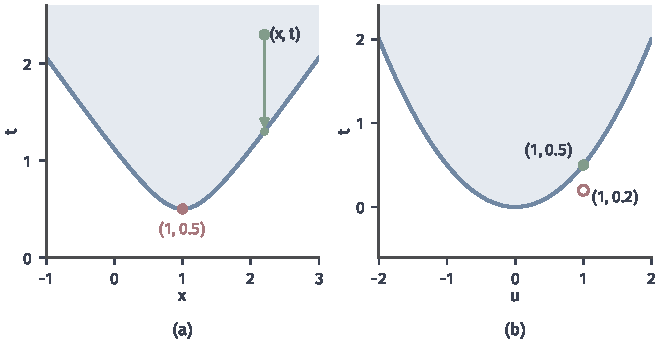
\includegraphics[width=112mm]{figures/05-optimization/06-constrained-optimization/matplotlib/cone-epigraph/figure.pdf}
  \caption{上图改写。(a)$f(x)=\lVert(x-1,1/2)\rVert_2$的上图（浅蓝），绿点下移到函数图像上时$t$减小而$x$不变，红点是上图中的最低点。(b)在网格上逐点判定$\lVert(2u,2t-1)\rVert_2\leq2t+1$，浅蓝区域恰是抛物线$t\geq u^2/2$的上方，绿点$(1,0.5)$在边界上，红色空心点$(1,0.2)$不满足约束。}
  \label{fig:cone-epigraph}
\end{BookInlineFigure}

\paragraph{凸二次目标}
平方范数多了一层：$\frac12\bm{x}^\top\bm{Q}\bm{x}\leq t$的左端是二次的，不是范数。这需要两步转换。

第一步是分解。$\bm{Q}\succeq\bm{0}$时存在$\bm{F}\in\mathbb{R}^{k\times n}$使$\bm{Q}=\bm{F}^\top\bm{F}$，例如取Cholesky因子或由谱分解得到。最小二乘中直接有$\bm{F}=\bm{D}$。于是上图约束是$\lVert\bm{F}\bm{x}\rVert_2^2\leq2t$。

第二步把“平方范数不超过乘积”写成二阶锥。

\begin{lemma}[旋转二阶锥]
\label{lem:cone-rotated-soc}
对$\bm{u}\in\mathbb{R}^k$和$s,w\in\mathbb{R}$，
\begin{equation}
 \lVert\bm{u}\rVert_2^2\leq sw,\quad s\geq0,\quad w\geq0
 \quad\Longleftrightarrow\quad
 \left\lVert\begin{bmatrix}2\bm{u}\\s-w\end{bmatrix}\right\rVert_2\leq s+w.
 \label{eq:cone-rotated-soc}
\end{equation}
\end{lemma}

\begin{proof}
先证从左到右。由$\lVert\bm{u}\rVert_2^2\leq sw$，
\[
 4\lVert\bm{u}\rVert_2^2+(s-w)^2\leq4sw+(s-w)^2=(s+w)^2.
\]
又$s+w\geq0$，两边开方得到右式。

再证从右到左。右式的范数不小于$\lvert s-w\rvert$，所以$s+w\geq\lvert s-w\rvert$。分别取绝对值的两种符号，得到$w\geq0$和$s\geq0$。把右式平方，同样的展开给出$4\lVert\bm{u}\rVert_2^2\leq4sw$。
\end{proof}

取$\bm{u}=\bm{F}\bm{x}$、$s=2t$、$w=1$，就得到$\lVert\bm{F}\bm{x}\rVert_2^2\leq2t$的二阶锥形式。凸二次规划~\eqref{eq:cone-qp}因而等价于
\begin{equation}
 \begin{aligned}
 \min_{\bm{x},t}\quad&t+\bm{q}^\top\bm{x}\\
 \text{s.t.}\quad&\left\lVert\begin{bmatrix}2\bm{F}\bm{x}\\2t-1\end{bmatrix}\right\rVert_2\leq2t+1,\\
 &\bm{A}\bm{x}=\bm{b},\quad\bm{G}\bm{x}\leq\bm{h}.
 \end{aligned}
 \label{eq:cone-qp-socp}
\end{equation}
图~\ref{fig:cone-epigraph}(b)用网格判定的方式核对了$k=1$的情形：约束$\lVert(2u,2t-1)\rVert_2\leq2t+1$的解集正好是$t\geq u^2/2$。

再用定义~\ref{def:cone-equivalent}核对。第一条取$t=\frac12\bm{x}^\top\bm{Q}\bm{x}$。第二条由引理得到$t\geq\frac12\bm{x}^\top\bm{Q}\bm{x}$，于是原目标不超过改写后的目标。恢复$\bm{x}$时丢弃$t$即可。

\begin{example}[预算问题的二阶锥形式]
\label{ex:cone-budget-socp}
预算问题的目标是$\frac12\lVert\bm{D}\bm{x}-\bm{r}\rVert_2^2$，这里取$\bm{u}=\bm{D}\bm{x}-\bm{r}$，约束写成
\[
 \left\lVert\begin{bmatrix}2(\bm{D}\bm{x}-\bm{r})\\2t-1\end{bmatrix}\right\rVert_2\leq2t+1.
\]
在$\bm{x}^\star=(3/2,1/2)$处，残差是$(-2,1/2,1/2)$，取$t=9/4$。左端向量是$(-4,1,1,7/2)$，长度的平方是
\[
 16+1+1+\frac{49}{4}=\frac{121}{4}.
\]
所以左端等于$11/2$，右端也等于$2t+1=11/2$。约束取等号，改写问题的目标值$t=9/4$与原问题的$f^\star$相同。
\end{example}

只有$\bm{Q}\succeq\bm{0}$时才有实分解$\bm{Q}=\bm{F}^\top\bm{F}$。第~\ref{sec:cone-nonconvex-qp}小节的$\operatorname{diag}(1,-1)$没有这样的分解，也不可能写成式~\eqref{eq:cone-qp-socp}：二阶锥规划的可行集是凸的，而目标的上图不凸。

另外，若目标是$\min\lVert\bm{D}\bm{x}-\bm{r}\rVert_2^2$，也可以直接最小化不带平方的范数。平方在非负数上严格递增，所以两者最优解相同；但最优值不同，这与定义~\ref{def:cone-equivalent}的“最优值相等”不是一回事，恢复目标值时要重新平方。

\paragraph{维数与成本}
增加变量并不自动带来计算上的好处。表~\ref{tab:cone-epi-cost}比较凸二次目标的两种写法，$\bm{Q}=\bm{F}^\top\bm{F}$，$\bm{F}\in\mathbb{R}^{k\times n}$。

\begin{BookInlineTable}
  \centering
  \begin{tabular}{lll}
    \toprule
    & 二次规划形式 & 二阶锥形式\\
    \midrule
    变量个数 & $n$ & $n+1$\\
    非线性结构 & 目标中的$\bm{Q}$ & 一个$k+2$维的二阶锥\\
    需要的准备 & $\bm{Q}$或矩阵向量积 & 分解$\bm{F}$\\
    可用的方法 & 二次规划专用方法 & 通用锥规划方法\\
    \bottomrule
  \end{tabular}
  \caption{同一凸二次目标的两种写法。}
  \label{tab:cone-epi-cost}
\end{BookInlineTable}

$\bm{Q}$稀疏时，分解因子$\bm{F}$可能比$\bm{Q}$稠密得多，改写后存储反而增加。$\bm{Q}$只能通过矩阵向量积访问时，分解根本做不出来。反过来，$\bm{Q}=\bm{D}^\top\bm{D}$稠密而$\bm{D}$稀疏时，直接用$\bm{F}=\bm{D}$比存$\bm{Q}$便宜。

改写的价值在于让问题能交给统一的求解方法，能和其他范数约束混用。只有二次目标和线性约束时，保留原形式通常更省。

\subsection{Schur补改写}
\label{sec:cone-schur}

二次上界和矩阵的逆都不是矩阵元素的线性函数。这一小节回答：这种限制能否写成线性矩阵不等式？工具是Schur补，关键是分清哪一块必须正定。

\paragraph{从配方到判据}
先看$2\times2$的情形。设$p>0$，考虑二次型
\[
 pa^2+2nab+Tb^2.
\]
配方得到
\[
 p\Bigl(a+\frac{n}{p}b\Bigr)^2+\Bigl(T-\frac{n^2}{p}\Bigr)b^2.
\]
第一项可以用$a$消成零，所以整个二次型非负，取决于第二项的系数$T-n^2/p$是否非负。

矩阵版本完全类似，只是把除以$p$换成乘以逆矩阵。

\begin{lemma}[Schur补判据]
\label{lem:cone-schur}
设对称矩阵分块为
\begin{equation}
 \bm{M}=\begin{bmatrix}\bm{P}&\bm{N}\\\bm{N}^\top&\bm{T}\end{bmatrix},
 \label{eq:cone-block-matrix}
\end{equation}
其中$\bm{P}\succ\bm{0}$。则
\begin{equation}
 \bm{M}\succeq\bm{0}\quad\Longleftrightarrow\quad\bm{T}-\bm{N}^\top\bm{P}^{-1}\bm{N}\succeq\bm{0}.
 \label{eq:cone-schur}
\end{equation}
矩阵$\bm{T}-\bm{N}^\top\bm{P}^{-1}\bm{N}$称为$\bm{P}$在$\bm{M}$中的\term{Schur补}（Schur complement）。
\end{lemma}

\begin{proof}
对任意向量$\bm{a},\bm{b}$，记$\bm{S}=\bm{T}-\bm{N}^\top\bm{P}^{-1}\bm{N}$。配方得到
\[
 \begin{bmatrix}\bm{a}\\\bm{b}\end{bmatrix}^\top\bm{M}\begin{bmatrix}\bm{a}\\\bm{b}\end{bmatrix}
 =(\bm{a}+\bm{P}^{-1}\bm{N}\bm{b})^\top\bm{P}(\bm{a}+\bm{P}^{-1}\bm{N}\bm{b})+\bm{b}^\top\bm{S}\bm{b}.
\]
若$\bm{S}\succeq\bm{0}$，右端两项都非负，$\bm{M}\succeq\bm{0}$。

反过来，设$\bm{M}\succeq\bm{0}$。对任意$\bm{b}$，取$\bm{a}=-\bm{P}^{-1}\bm{N}\bm{b}$，第一项变为零，于是$\bm{b}^\top\bm{S}\bm{b}\geq0$。
\end{proof}

式~\eqref{eq:cone-schur}的左端对$\bm{P},\bm{N},\bm{T}$是线性的，右端含有逆和乘积。这就是改写的用处：把弯曲的右端换成线性的左端。

\paragraph{二次型上界}
令$\bm{P}=\bm{I}$、$\bm{N}=\bm{u}$、$\bm{T}=t$，由引理~\ref{lem:cone-schur}，
\begin{equation}
 \lVert\bm{u}\rVert_2^2\leq t\quad\Longleftrightarrow\quad\begin{bmatrix}\bm{I}&\bm{u}\\\bm{u}^\top&t\end{bmatrix}\succeq\bm{0}.
 \label{eq:cone-schur-quadratic}
\end{equation}
代入$\bm{u}=\bm{D}\bm{x}-\bm{r}$，左端对$\bm{x}$是二次的，右端的矩阵对$(\bm{x},t)$却是仿射的。这条约束就是一条线性矩阵不等式，和式~\eqref{eq:cone-lmi}同型。这里单位块$\bm{I}$恒正定，引理的条件自动满足。

以预算问题的解为例，$\lVert\bm{u}\rVert_2^2=9/2$。取$t=9/2$，矩阵是$4\times4$的，它的Schur补为零，矩阵半正定且奇异。取$t$更小，Schur补为负，矩阵不再半正定。

\paragraph{含逆矩阵的限制}
再看一个$\bm{P}$本身是变量的例子。设$\bm{Y}\succ\bm{0}$是对称矩阵变量，$\bm{b}$是向量，由引理~\ref{lem:cone-schur}，
\begin{equation}
 \bm{b}^\top\bm{Y}^{-1}\bm{b}\leq t\quad\Longleftrightarrow\quad\begin{bmatrix}\bm{Y}&\bm{b}\\\bm{b}^\top&t\end{bmatrix}\succeq\bm{0}\qquad(\bm{Y}\succ\bm{0}).
 \label{eq:cone-schur-inverse}
\end{equation}
右端是$(\bm{Y},\bm{b},t)$的线性矩阵不等式，也说明左端的函数在$\bm{Y}\succ\bm{0}$上对$(\bm{Y},\bm{b})$联合凸：它的上图由一条线性矩阵不等式定义。

用数值走一遍。取
\[
 \bm{Y}=\begin{bmatrix}2&1\\1&2\end{bmatrix},\qquad\bm{b}=\begin{bmatrix}1\\1\end{bmatrix}.
\]
矩阵的逆是
\[
 \bm{Y}^{-1}=\frac13\begin{bmatrix}2&-1\\-1&2\end{bmatrix}.
\]
代入得到
\[
 \bm{b}^\top\bm{Y}^{-1}\bm{b}=\frac13(2-1-1+2)=\frac23.
\]
$3\times3$块矩阵的行列式等于$\det\bm{Y}$与Schur补的乘积，
\[
 \det\bm{M}=3\Bigl(t-\frac23\Bigr).
\]
于是$t<2/3$时矩阵不半正定，$t=2/3$时恰好在边界上。数值上，$t=1/2$时最小特征值约为$-0.137$，$t=1$时约为$0.268$。图~\ref{fig:cone-schur}(a)画出最小特征值穿过零点的过程。

\begin{BookInlineFigure}
  \centering
  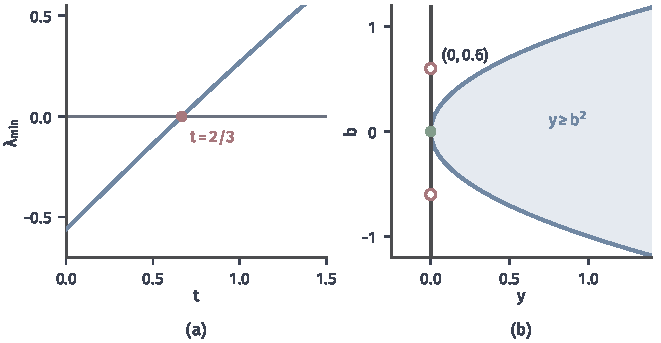
\includegraphics[width=112mm]{figures/05-optimization/06-constrained-optimization/matplotlib/cone-schur/figure.pdf}
  \caption{Schur补判据及其边界。(a)式~\eqref{eq:cone-schur-inverse}的块矩阵的最小特征值随$t$的变化，红点是$t=2/3$。(b)$\begin{bmatrix}y&b\\b&1\end{bmatrix}\succeq\bm{0}$的解集（浅蓝）是抛物线$y\geq b^2$的内部及边界。深灰线$y=0$上只有绿点$(0,0)$可行，红色空心点$(0,\pm0.6)$不可行。}
  \label{fig:cone-schur}
\end{BookInlineFigure}

\paragraph{奇异的情形}
$\bm{P}$只半正定时，不能写$\bm{P}^{-1}$，把逆换成伪逆也不够。看一个例子：
\[
 \begin{bmatrix}0&1\\1&1\end{bmatrix}.
\]
这里$\bm{P}=0$，伪逆也是$0$，“Schur补”算出来是$1\geq0$。但矩阵的行列式是$-1$，它不半正定。缺的是一个像空间的条件：$\bm{P}$的零方向上，$\bm{N}$也必须为零。

\begin{lemma}[奇异情形的Schur补判据]
\label{lem:cone-schur-singular}
在引理~\ref{lem:cone-schur}的分块中，设$\bm{P}\succeq\bm{0}$，$\bm{P}^\dagger$是其伪逆。则$\bm{M}\succeq\bm{0}$，当且仅当
\begin{equation}
 (\bm{I}-\bm{P}\bm{P}^\dagger)\bm{N}=\bm{0}\quad\text{且}\quad\bm{T}-\bm{N}^\top\bm{P}^\dagger\bm{N}\succeq\bm{0}.
 \label{eq:cone-schur-singular}
\end{equation}
\end{lemma}

\begin{proof}
设$\bm{M}\succeq\bm{0}$。任取$\bm{w}\in\ker\bm{P}$和向量$\bm{v}$，把$\bm{M}$的二次型作用在$(\bm{w},\varepsilon\bm{v})$上，得到
\[
 2\varepsilon\bm{w}^\top\bm{N}\bm{v}+\varepsilon^2\bm{v}^\top\bm{T}\bm{v}\geq0.
\]
这对正负的小$\varepsilon$都成立，必有$\bm{w}^\top\bm{N}\bm{v}=0$。所以$\bm{N}$的列与$\ker\bm{P}$正交，属于$\operatorname{range}\bm{P}$，这正是$\bm{P}\bm{P}^\dagger\bm{N}=\bm{N}$。

在条件$\bm{P}\bm{P}^\dagger\bm{N}=\bm{N}$之下，令
\[
 \bm{U}=\begin{bmatrix}\bm{I}&-\bm{P}^\dagger\bm{N}\\\bm{0}&\bm{I}\end{bmatrix},
\]
它可逆。直接相乘，并用$\bm{P}^\dagger\bm{P}\bm{P}^\dagger=\bm{P}^\dagger$，得到
\[
 \bm{U}^\top\bm{M}\bm{U}=\begin{bmatrix}\bm{P}&\bm{0}\\\bm{0}&\bm{T}-\bm{N}^\top\bm{P}^\dagger\bm{N}\end{bmatrix}.
\]
可逆合同变换保持半正定性，所以$\bm{M}\succeq\bm{0}$当且仅当右端半正定，也就是第二个条件成立。这同时完成了两个方向的证明。
\end{proof}

图~\ref{fig:cone-schur}(b)展示了这个条件的几何含义。$\begin{bmatrix}y&b\\b&1\end{bmatrix}\succeq\bm{0}$在$y>0$时等价于$b^2/y\leq1$，即$y\geq b^2$。到$y=0$时，$b^2/y$没有定义，判据要求$b=0$，图中只有原点留下。

这里还有一个定义域的问题。式~\eqref{eq:cone-schur-inverse}要求$\bm{Y}\succ\bm{0}$，而块矩阵半正定只推出$\bm{Y}\succeq\bm{0}$。改写时若丢掉严格正定的要求，集合就多了边界上的奇异$\bm{Y}$，这些点在原问题中$\bm{Y}^{-1}$并无定义。这时要么说明原函数在边界上取什么值，要么在求解后核对$\bm{Y}$是否真的正定。

\paragraph{二阶锥也是线性矩阵不等式}
同样的工具给出
\begin{equation}
 \lVert\bm{u}\rVert_2\leq t\quad\Longleftrightarrow\quad\begin{bmatrix}t\bm{I}&\bm{u}\\\bm{u}^\top&t\end{bmatrix}\succeq\bm{0}.
 \label{eq:cone-soc-as-lmi}
\end{equation}
$t>0$时由引理~\ref{lem:cone-schur}，Schur补是$t-\bm{u}^\top\bm{u}/t$。$t=0$时左上块为零，由引理~\ref{lem:cone-schur-singular}迫使$\bm{u}=\bm{0}$。$t<0$时对角元为负，矩阵不半正定。三种情形都与左式一致。

所以二阶锥规划可以写成半正定规划。这种包含关系的计算含义留到第~\ref{sec:cone-methods}节讨论。

\section{半正定松弛}
\label{sec:cone-relax}

第~\ref{sec:cone-nonconvex-qp}小节的问题不能等价地改写成凸问题，KKT条件也给不出全局证书。既然改不成凸问题，能否算出一个有保证的下界，用它判断手上的候选解离最优还有多远？

\paragraph{把乘积收集到矩阵里}
考虑\term{二次约束二次规划}（quadratically constrained quadratic program，QCQP）
\begin{equation}
 \begin{aligned}
 \min_{\bm{x}\in\mathbb{R}^n}\quad&\bm{x}^\top\bm{Q}_0\bm{x}+2\bm{q}_0^\top\bm{x}+c_0\\
 \text{s.t.}\quad&\bm{x}^\top\bm{Q}_i\bm{x}+2\bm{q}_i^\top\bm{x}+c_i\leq0,\quad i=1,\ldots,m,
 \end{aligned}
 \label{eq:cone-qcqp}
\end{equation}
其中$\bm{Q}_i$对称，可以不定。等式约束可以拆成两条不等式，因此这里只写不等式。

难点全在乘积$x_ix_j$上。这些乘积在$\bm{x}$上是非线性的，但只要把它们看成新的未知数，每个二次式都变成新未知数的线性函数。这就像把一笔难算的账换一种记法：先不管各项之间的关系，只把用到的项登记下来，账立刻变成加法。这个类比的边界是：各项之间的关系并没有消失，它们藏在下面矩阵的结构里，后面要单独处理。

具体做法是引入带常数坐标的矩阵
\begin{equation}
 \bm{Y}=\begin{bmatrix}1\\\bm{x}\end{bmatrix}\begin{bmatrix}1\\\bm{x}\end{bmatrix}^\top=\begin{bmatrix}1&\bm{x}^\top\\\bm{x}&\bm{x}\bm{x}^\top\end{bmatrix}\in\mathcal{S}^{n+1},
 \label{eq:cone-lift-matrix}
\end{equation}
行列下标从$0$开始。常数坐标的作用是把线性项和常数项也放进矩阵。记
\[
 \bm{M}_i=\begin{bmatrix}c_i&\bm{q}_i^\top\\\bm{q}_i&\bm{Q}_i\end{bmatrix},
\]
直接展开迹内积，得到
\begin{equation}
 \bm{x}^\top\bm{Q}_i\bm{x}+2\bm{q}_i^\top\bm{x}+c_i=\langle\bm{M}_i,\bm{Y}\rangle.
 \label{eq:cone-lift-linear}
\end{equation}
原来的二次式成了$\bm{Y}$的线性函数。

图~\ref{fig:cone-lift}以式~\eqref{eq:cone-nonconvex-objective}为例。这时$\bm{Q}_0=\operatorname{diag}(1/2,-1/2)$，$\bm{q}_0=(0,1/8)$，$c_0=0$。

\begin{BookInlineFigure}
  \centering
  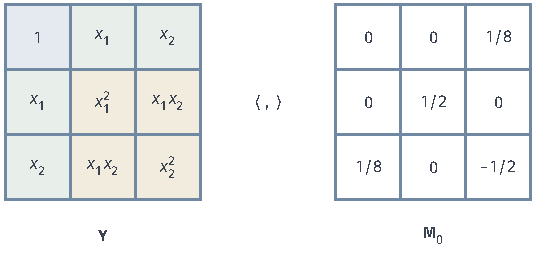
\includegraphics[width=90mm]{figures/05-optimization/06-constrained-optimization/tikz/cone-lift/figure.pdf}
  \caption{提升矩阵与目标系数。左边是$n=2$时的$\bm{Y}$，浅蓝格是常数，绿格是一次项，黄格是二次项。右边是目标$\frac12x_1^2-\frac12x_2^2+\frac14x_2$对应的$\bm{M}_0$，交叉项的系数对半分在两个对称位置上。二者的迹内积就是目标。}
  \label{fig:cone-lift}
\end{BookInlineFigure}

\paragraph{哪些矩阵来自向量}
不是每个矩阵都有式~\eqref{eq:cone-lift-matrix}的形状。下面的引理精确地指出需要哪些条件。

\begin{lemma}[秩一刻画]
\label{lem:cone-rank-one}
$\bm{Y}\in\mathcal{S}^{n+1}$具有式~\eqref{eq:cone-lift-matrix}的形状，当且仅当
\begin{equation}
 \bm{Y}\succeq\bm{0},\qquad Y_{0,0}=1,\qquad\operatorname{rank}\bm{Y}=1.
 \label{eq:cone-rank-one}
\end{equation}
\end{lemma}

\begin{proof}
式~\eqref{eq:cone-lift-matrix}的矩阵满足这三条：它是一个向量与自身的外积，秩为一且半正定，第一个元素是$1$。反过来，秩一半正定矩阵可以写成$\bm{Y}=\bm{v}\bm{v}^\top$。由$Y_{0,0}=v_0^2=1$得$v_0=\pm1$，必要时把$\bm{v}$换成$-\bm{v}$，可设$v_0=1$。记$\bm{v}=(1,\bm{x})$，$\bm{Y}$就有所要的形状。
\end{proof}

于是问题~\eqref{eq:cone-qcqp}等价于在条件~\eqref{eq:cone-rank-one}和$\langle\bm{M}_i,\bm{Y}\rangle\leq0$下最小化$\langle\bm{M}_0,\bm{Y}\rangle$。目标和约束都是线性的，半正定和$Y_{0,0}=1$也是凸约束，全部困难集中在秩一这一条上。

把它删掉，就得到\term{半正定松弛}（semidefinite relaxation）
\begin{equation}
 \begin{aligned}
 \min_{\bm{Y}\in\mathcal{S}^{n+1}}\quad&\langle\bm{M}_0,\bm{Y}\rangle\\
 \text{s.t.}\quad&\langle\bm{M}_i,\bm{Y}\rangle\leq0,\quad i=1,\ldots,m,\\
 &Y_{0,0}=1,\quad\bm{Y}\succeq\bm{0}.
 \end{aligned}
 \label{eq:cone-sdr}
\end{equation}

\subsection{松弛下界}
\label{sec:cone-relax-bound}

删掉一个约束，最优值只会变小。这一小节要把这件事写准确，并弄清楚上面的几步各自改变了什么。

\begin{theorem}[松弛给出下界]
\label{thm:cone-sdr-bound}
记问题~\eqref{eq:cone-qcqp}的最优值为$f^\star$，问题~\eqref{eq:cone-sdr}的最优值为$p_{\mathrm{rel}}$。则
\begin{equation}
 p_{\mathrm{rel}}\leq f^\star.
 \label{eq:cone-sdr-bound}
\end{equation}
\end{theorem}

\begin{proof}
任取问题~\eqref{eq:cone-qcqp}的可行点$\bm{x}$，按式~\eqref{eq:cone-lift-matrix}构造$\bm{Y}$。由引理~\ref{lem:cone-rank-one}，$\bm{Y}\succeq\bm{0}$且$Y_{0,0}=1$。由式~\eqref{eq:cone-lift-linear}，$\langle\bm{M}_i,\bm{Y}\rangle\leq0$，且$\langle\bm{M}_0,\bm{Y}\rangle$等于原目标值。所以$\bm{Y}$对问题~\eqref{eq:cone-sdr}可行，$p_{\mathrm{rel}}$不超过原目标值。对所有可行$\bm{x}$取下确界，即得结论。
\end{proof}

这个结论只用到定义~\ref{def:cone-equivalent}的第一条。第二条在这里不成立，因为松弛问题的可行矩阵不一定对应任何$\bm{x}$。表~\ref{tab:cone-relax-steps}把三步分开。

\begin{BookInlineTable}
  \centering
  \begin{tabular}{lll}
    \toprule
    步骤 & 做了什么 & 与原问题的关系\\
    \midrule
    提升 & 用$\bm{Y}$表示乘积，保留秩一 & 等价\\
    放松秩约束 & 删去$\operatorname{rank}\bm{Y}=1$ & 可行集变大，得到下界\\
    求解松弛 & 数值计算SDP & 近似解，下界需验证\\
    \bottomrule
  \end{tabular}
  \caption{半正定松弛的三个步骤。只有第一步不改变问题。}
  \label{tab:cone-relax-steps}
\end{BookInlineTable}

\begin{example}[松弛证明全局最优]
\label{ex:cone-relax-nonconvex}
回到目标~\eqref{eq:cone-nonconvex-objective}。可行集$-1\leq x_2\leq1$写成二次约束$x_2^2\leq1$。记$\bm{Y}$的元素
\[
 \bm{Y}=\begin{bmatrix}1&y_1&y_2\\y_1&X_{1,1}&X_{1,2}\\y_2&X_{1,2}&X_{2,2}\end{bmatrix}.
\]
松弛问题是在$X_{2,2}\leq1$、$\bm{Y}\succeq\bm{0}$下最小化
\[
 \frac12X_{1,1}-\frac12X_{2,2}+\frac14y_2.
\]

下面逐项估计目标。半正定矩阵的对角元非负，所以$X_{1,1}\geq0$。约束给出$X_{2,2}\leq1$。再由$\{0,2\}$行列对应的$2\times2$主子式非负，$y_2^2\leq X_{2,2}\leq1$，所以$y_2\geq-1$。三项合起来，
\[
 \frac12X_{1,1}-\frac12X_{2,2}+\frac14y_2\geq0-\frac12-\frac14=-\frac34.
\]
这个下界由点A对应的秩一矩阵取到，所以$p_{\mathrm{rel}}=-3/4$，也就是$f^\star=-3/4$。KKT条件区分不开A和B，松弛却直接证明了A是全局最优，而B的目标值$-1/4$高于下界，不是全局最优。
\end{example}

\paragraph{符号变量}
下面这个问题里，松弛一般不紧。设$\bm{W}\in\mathcal{S}^n$，考虑
\begin{equation}
 \min_{\bm{x}}\ \bm{x}^\top\bm{W}\bm{x}\quad\text{s.t.}\quad x_i^2=1,\quad i=1,\ldots,n.
 \label{eq:cone-sign-problem}
\end{equation}
变量只能取$\pm1$，这是一个把点分到两侧的组合问题。约束$x_i^2=1$恰好是二次的，提升后成为对角线上的线性条件，一条也不丢。

这里没有线性项，$\bm{Y}$中的$\bm{x}$块可以去掉。设$\bm{Y}$可行，记其$\bm{x}$块为$\hat{\bm{x}}$，令$\bm{D}_{\pm}=\operatorname{diag}(1,-\bm{I})$。矩阵$\bm{D}_{\pm}\bm{Y}\bm{D}_{\pm}$也可行，目标不变，只是$\hat{\bm{x}}$变号。二者的平均仍可行，而$\bm{x}$块为零。所以只需保留右下块$\bm{X}=\bm{x}\bm{x}^\top$，松弛写成
\begin{equation}
 \min_{\bm{X}\in\mathcal{S}^n}\ \langle\bm{W},\bm{X}\rangle\quad\text{s.t.}\quad X_{i,i}=1,\quad i=1,\ldots,n,\quad\bm{X}\succeq\bm{0}.
 \label{eq:cone-sign-relax}
\end{equation}
取$\bm{A}_i=\bm{e}_i\bm{e}_i^\top$、$b_i=1$，由式~\eqref{eq:cone-sdp-dual}，它的对偶问题是
\begin{equation}
 \max_{\bm{y}\in\mathbb{R}^n}\ \sum_{i=1}^ny_i\quad\text{s.t.}\quad\bm{W}-\operatorname{diag}(\bm{y})\succeq\bm{0}.
 \label{eq:cone-sign-dual}
\end{equation}

先看$n=2$，$\bm{W}$的对角元为零、非对角元为$1$。松弛的可行矩阵是$\begin{bmatrix}1&a\\a&1\end{bmatrix}$，$a\in[-1,1]$，目标是$2a$。最优在$a=-1$取到，矩阵秩一，对应$\bm{x}=(1,-1)$，松弛是紧的。

再看三角形的例子。取$n=3$，
\[
 \bm{W}=\begin{bmatrix}0&1&1\\1&0&1\\1&1&0\end{bmatrix}.
\]
目标是$2(x_1x_2+x_1x_3+x_2x_3)$。枚举$8$个符号组合，全同时目标为$6$，其余都是两个相同、一个相反，目标为$-2$。所以$f^\star=-2$。

松弛问题中取
\[
 \hat{\bm{X}}=\begin{bmatrix}1&-1/2&-1/2\\-1/2&1&-1/2\\-1/2&-1/2&1\end{bmatrix}.
\]
它的特征值是$0,3/2,3/2$，半正定，对角元都是$1$，所以松弛可行。六个非对角元各贡献$-1/2$，目标是
\[
 \langle\bm{W},\hat{\bm{X}}\rangle=-3.
\]

再看对偶问题~\eqref{eq:cone-sign-dual}。取$\bm{y}=(-1,-1,-1)$，则
\[
 \bm{W}-\operatorname{diag}(\bm{y})=\bm{W}+\bm{I}=\bm{1}\bm{1}^\top\succeq\bm{0},
\]
对偶目标是$-3$。原始和对偶的值相等，所以$p_{\mathrm{rel}}=-3$。

下界$-3$比真实最优值$-2$低了$1$，这个间隙来自放松秩约束，而不是求解误差。图~\ref{fig:cone-relax-slice}在切片上画出了可行集究竟扩大了多少。

\begin{BookInlineFigure}
  \centering
  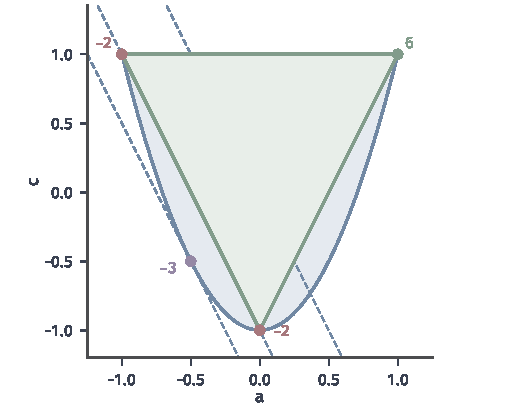
\includegraphics[width=88mm]{figures/05-optimization/06-constrained-optimization/matplotlib/cone-relax-slice/figure.pdf}
  \caption{$n=3$时松弛可行集在切片$X_{1,2}=X_{1,3}=a$、$X_{2,3}=c$上的形状。浅蓝抛物线区域$2a^2-1\leq c\leq1$是松弛的可行集。绿色三角形是秩一矩阵（符号解）的凸包，其顶点旁标注目标$4a+2c$的值。蓝色虚线是等值线，紫点是松弛最优解，目标$-3$，它在三角形之外。}
  \label{fig:cone-relax-slice}
\end{BookInlineFigure}

切片的形状可以直接算出来。矩阵$\begin{bmatrix}1&a&a\\a&1&c\\a&c&1\end{bmatrix}$有特征向量$(0,1,-1)$，特征值$1-c$，要求$c\leq1$。在与之正交的子空间上，矩阵约化为$\begin{bmatrix}1&\sqrt2a\\\sqrt2a&1+c\end{bmatrix}$，半正定要求$1+c\geq2a^2$。

\subsection{原解恢复}
\label{sec:cone-relax-recovery}

松弛的解是矩阵，原问题要的是向量。这一小节回答：什么时候可以把向量直接读出来，读不出来时又该怎么办？

\paragraph{秩一的情形}
若松弛的最优矩阵恰好秩一，问题就结束了。

\begin{theorem}[秩一解恢复原问题的最优解]
\label{thm:cone-rank-one-exact}
设$\bm{Y}^\star$是问题~\eqref{eq:cone-sdr}的最优解，且$\operatorname{rank}\bm{Y}^\star=1$。取$\bm{x}^\star$为$\bm{Y}^\star$第$0$列的后$n$个元素。则$\bm{x}^\star$是问题~\eqref{eq:cone-qcqp}的全局最优解，且$p_{\mathrm{rel}}=f^\star$。
\end{theorem}

\begin{proof}
由引理~\ref{lem:cone-rank-one}，$\bm{Y}^\star$具有式~\eqref{eq:cone-lift-matrix}的形状，其中的向量就是$\bm{x}^\star$。由式~\eqref{eq:cone-lift-linear}，$\bm{x}^\star$满足全部约束，目标值等于$p_{\mathrm{rel}}$。结合式~\eqref{eq:cone-sdr-bound}，
\[
 f(\bm{x}^\star)=p_{\mathrm{rel}}\leq f^\star\leq f(\bm{x}^\star).
\]
所以三者相等。
\end{proof}

定理依赖于约束的对应关系：松弛必须把原问题的每条约束都按式~\eqref{eq:cone-lift-linear}写了进去。若为了省事删掉了某条约束，恢复的$\bm{x}^\star$还要单独检查这条约束。

\paragraph{高秩的情形}
矩阵的秩大于$1$时，它不是任何向量的外积，松弛的最优矩阵不是原问题的可行解。这时要把矩阵“变回”向量，常用两种办法：取最大特征值对应的特征向量作投影；或者把矩阵分解后随机取整。无论哪一种，都是问题专属的启发式步骤。

对符号问题，常用的取整步骤如下\scite{goemans1995maxcut}。把$\bm{X}$分解成$X_{i,j}=\bm{v}_i^\top\bm{v}_j$，$\bm{v}_i$是单位向量，因为对角元是$1$。随机抽取一个标准高斯向量$\bm{g}$，令
\begin{equation}
 x_i=\operatorname{sign}(\bm{v}_i^\top\bm{g}).
 \label{eq:cone-rounding}
\end{equation}
几何上，这是用一个随机的超平面把各个单位向量分成两侧，同侧的$x_i$相同。

两个向量被分开的概率与它们的夹角成正比。$\bm{g}$在$\bm{v}_i,\bm{v}_j$所在平面上的投影方向是均匀的，夹角为$\theta$时被分开的概率是$\theta/\pi$。于是
\begin{equation}
 \mathbb{E}[x_ix_j]=1-\frac{2\theta}{\pi}=\frac{2}{\pi}\arcsin X_{i,j}.
 \label{eq:cone-rounding-expectation}
\end{equation}
最后一步用了$\theta=\arccos X_{i,j}$和$\arcsin z=\pi/2-\arccos z$。

三角形的$\hat{\bm{X}}$可以分解成平面上三个互成$120^\circ$的单位向量，见图~\ref{fig:cone-round-vectors}(a)。任何一条过原点的直线都把三个向量分成一个和两个。所以取整结果总是两同一异，目标总是$-2$，碰巧等于$f^\star$。由式~\eqref{eq:cone-rounding-expectation}验证，$\mathbb{E}[x_ix_j]=-1/3$，目标的期望是$6\cdot(-1/3)=-2$。

\begin{BookInlineFigure}
  \centering
  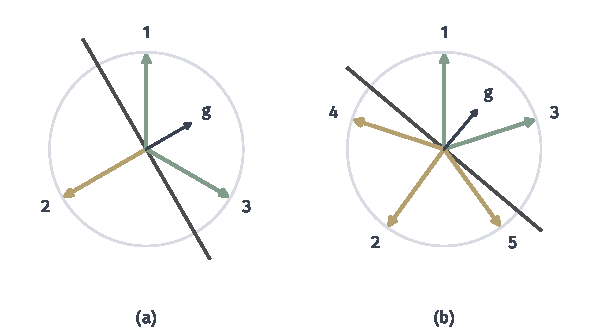
\includegraphics[width=100mm]{figures/05-optimization/06-constrained-optimization/matplotlib/cone-round-vectors/figure.pdf}
  \caption{随机超平面取整。深灰线是与随机方向$\bm{g}$垂直的直线，绿色向量对应$x_i=1$，黄色向量对应$x_i=-1$。(a)三角形问题的三个向量互成$120^\circ$。(b)五边形问题的五个向量，相邻编号之间夹角$144^\circ$。}
  \label{fig:cone-round-vectors}
\end{BookInlineFigure}

\paragraph{恢复可能破坏可行性}
取整会改变目标，也会破坏约束。设问题~\eqref{eq:cone-sign-problem}中$n=4$，再加上平衡约束$x_1+x_2+x_3+x_4=0$。把它平方后提升为$\langle\bm{1}\bm{1}^\top,\bm{X}\rangle=0$。矩阵
\[
 \bm{X}=\frac43\bm{I}-\frac13\bm{1}\bm{1}^\top
\]
对角元为$1$，非对角元为$-1/3$，特征值是$4/3,4/3,4/3,0$，且$\langle\bm{1}\bm{1}^\top,\bm{X}\rangle=4-12/3=0$，满足松弛的全部约束。

它对应四面体的四个顶点方向，这四个向量和为零，一个超平面不可能把它们全放在同一侧，取整结果只有两种：二比二（满足平衡约束）或一比三（$(\sum_ix_i)^2=4$，违反约束）。由式~\eqref{eq:cone-rounding-expectation}，
\[
 \mathbb{E}\Bigl[\bigl(\sum_ix_i\bigr)^2\Bigr]=4+12\cdot\frac2\pi\arcsin\Bigl(-\frac13\Bigr)\approx1.404.
\]
除以$4$，一比三的概率约为$0.351$。超过三分之一的取整结果是不可行的，必须修复或丢弃后重新检验。

\subsection{上下界检验}
\label{sec:cone-relax-bounds}

松弛算出来的数字到底保证了什么？这一小节把上界、下界和间隙分别交代清楚。

\paragraph{两个界}
一个经过原约束核对的点$\hat{\bm{x}}$给出上界$U=f(\hat{\bm{x}})$。一个松弛的对偶可行解$\bm{y}$给出下界$L$，对符号问题就是$L=\sum_iy_i$。合起来是一条链：
\begin{equation}
 L\leq p_{\mathrm{rel}}\leq f^\star\leq U.
 \label{eq:cone-bound-chain}
\end{equation}
报告时写出$U-L$。它同时包含松弛自身的间隙和求解的误差，是对$\hat{\bm{x}}$质量的一个可靠估计。

在三角形例子中，$U=-2$，$L=-3$，$U-L=1$。这里$\hat{\bm{x}}$其实已经最优，间隙全部来自松弛，继续迭代也不会缩小。间隙不为零，不代表候选解不好。

\paragraph{近似原始值不是下界}
常见的错误是把松弛问题的一个可行矩阵的目标值当作下界。式~\eqref{eq:cone-bound-chain}中排在$f^\star$左边的是$p_{\mathrm{rel}}$，而可行矩阵$\hat{\bm{X}}$的目标值满足的是
\[
 \langle\bm{W},\hat{\bm{X}}\rangle\geq p_{\mathrm{rel}},
\]
方向相反。它可以高于$f^\star$。

取三角形问题中对角元为$1$、非对角元为$-0.3$的矩阵，特征值是$0.4,1.3,1.3$，松弛可行，目标是$-1.8$。可$f^\star=-2<-1.8$。若把$-1.8$当作下界，就会错误地断言符号问题的最优值不低于$-1.8$，如图~\ref{fig:cone-bounds-line}所示。

\begin{BookInlineFigure}
  \centering
  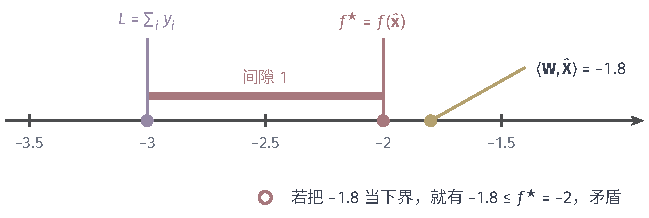
\includegraphics[width=110mm]{figures/05-optimization/06-constrained-optimization/tikz/cone-bounds-line/figure.pdf}
  \caption{三角形符号问题的各个数值。紫点是对偶可行解给出的下界$L=-3$，红点是最优值$f^\star=-2$，它也等于取整解的上界。黄点是松弛的一个未收敛可行矩阵的目标值$-1.8$，位于$f^\star$右侧，不能当作下界。红色粗线是报告的间隙。}
  \label{fig:cone-bounds-line}
\end{BookInlineFigure}

\paragraph{从近似对偶解得到有效下界}
数值求解器返回的$\bm{y}$往往只是近似可行，$\bm{W}-\operatorname{diag}(\bm{y})$可能有微小的负特征值，严格说来式~\eqref{eq:cone-bound-chain}不能用。幸好符号问题的对偶可行性很容易修复。

\begin{lemma}[修复对偶可行性]
\label{lem:cone-repair-dual}
对任意$\bm{y}\in\mathbb{R}^n$，记$\lambda$为矩阵$\bm{W}-\operatorname{diag}(\bm{y})$的最小特征值。则
\begin{equation}
 L(\bm{y})=\sum_{i=1}^ny_i+n\lambda
 \label{eq:cone-repaired-bound}
\end{equation}
是问题~\eqref{eq:cone-sign-relax}的最优值的下界，因而也是$f^\star$的下界。
\end{lemma}

\begin{proof}
令$\bm{y}'=\bm{y}+\lambda\bm{1}$。则
\[
 \bm{W}-\operatorname{diag}(\bm{y}')=\bm{W}-\operatorname{diag}(\bm{y})-\lambda\bm{I}\succeq\bm{0},
\]
因为最小特征值被平移到了零。所以$\bm{y}'$是问题~\eqref{eq:cone-sign-dual}的可行解，目标是$\sum_iy_i+n\lambda$。由弱对偶和定理~\ref{thm:cone-sdr-bound}得到结论。
\end{proof}

这个界对任何$\bm{y}$都成立，只要算得出最小特征值。例如在三角形问题中取不可行的$\bm{y}=(-1.1,-0.9,-1)$，最小特征值约为$-0.059$，修复后$L\approx-3.177$，仍是有效的下界。数值计算特征值本身有误差，严格的报告还要再减去一个反映舍入误差的小量。

图~\ref{fig:cone-bounds-iter}是一个$10$个变量的符号问题，权重是固定种子生成的$\pm1$。枚举全部符号组合得到$f^\star=-46$。求解松弛时，绿线是原始可行矩阵的目标值，紫线是由式~\eqref{eq:cone-repaired-bound}修复的下界。

\begin{BookInlineFigure}
  \centering
  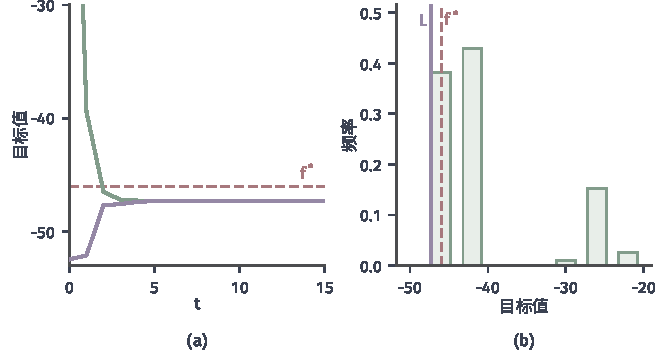
\includegraphics[width=112mm]{figures/05-optimization/06-constrained-optimization/matplotlib/cone-bounds-iter/figure.pdf}
  \caption{$n=10$的符号问题（$\bm{W}$的非对角元为随机$\pm1$，种子$7$）。(a)松弛的求解过程：绿线是可行矩阵的目标值，紫线是修复后的对偶下界，红色虚线是枚举得到的$f^\star=-46$。前两步绿线高于$f^\star$，不是$f^\star$的下界；收敛后二者相遇在$L\approx-47.28$。(b)从最终矩阵取整$2000$次得到的目标值分布，紫线是$L$，红色虚线是$f^\star$。}
  \label{fig:cone-bounds-iter}
\end{BookInlineFigure}

绿线在开始两步高于$f^\star$，把它当下界会得到错误的结论。收敛后两条线都停在$-47.28$附近，这就是$p_{\mathrm{rel}}$，它比$f^\star$低约$1.28$。这段距离是放松秩约束的代价，再多的迭代也消除不了。

图的(b)部分取整$2000$次。约$38\%$的试验得到$-46$，也就是真实最优值；其余的目标更差，最差到$-22$。所以取整要重复多次，取其中最好的可行点作为上界。这里$U=-46$，$U-L\approx1.28$，已经足以说明候选解很接近最优。

表~\ref{tab:cone-reported-quantities}整理了各个量的含义和要做的核对。

\begin{BookInlineTable}
  \centering
  \begin{tabular}{lll}
    \toprule
    量 & 保证 & 需要核对\\
    \midrule
    $f(\hat{\bm{x}})$ & $f^\star$的上界 & $\hat{\bm{x}}$满足原约束\\
    $\sum_iy_i$ & $f^\star$的下界 & $\bm{y}$对偶可行\\
    $\langle\bm{W},\hat{\bm{X}}\rangle$ & 收敛时接近$p_{\mathrm{rel}}$ & 不是$f^\star$的界\\
    $U-L$ & 候选解的最优性间隙 & 上下两界都已核对\\
    \bottomrule
  \end{tabular}
  \caption{半正定松弛的结果中各个量的含义。}
  \label{tab:cone-reported-quantities}
\end{BookInlineTable}

\section{模型与求解方法}
\label{sec:cone-methods}

同一个问题可以有多种写法。于是要问：写法不同时，变量规模、存储和运算量分别差多少，应该按什么选择？

\paragraph{同一个问题的三种写法}
预算问题已经写过三遍：原变量的二次规划、式~\eqref{eq:cone-qp-socp}的二阶锥形式，以及用式~\eqref{eq:cone-schur-quadratic}得到的线性矩阵不等式。三者等价，解都是$(3/2,1/2)$，规模却不同。表~\ref{tab:cone-three-forms}列出例子（$n=2$，$k=3$）和一般情形。

\begin{BookInlineTable}
  \centering
  \begin{tabular}{llll}
    \toprule
    & 二次规划 & 二阶锥形式 & 线性矩阵不等式\\
    \midrule
    变量 & $2$（一般$n$） & $3$（$n+1$） & $3$（$n+1$）\\
    非线性结构 & $\bm{Q}$，$2\times2$ & $5$维锥（$k+2$） & $4\times4$（$k+1$阶）\\
    矩阵独立元素 & $3$ & 无 & $10$\\
    恢复原变量 & 直接 & 丢弃$t$ & 丢弃$t$\\
    \bottomrule
  \end{tabular}
  \caption{预算问题的三种等价写法。括号内是一般规模：$n$个变量，$\bm{F}\in\mathbb{R}^{k\times n}$。线性约束三者相同，未列出。}
  \label{tab:cone-three-forms}
\end{BookInlineTable}

\paragraph{模型的包含关系}
图~\ref{fig:cone-hierarchy}把前面的改写连成一条链。线性规划是$\bm{Q}=\bm{0}$的二次规划；凸二次规划由式~\eqref{eq:cone-qp-socp}写成二阶锥规划；二阶锥规划由式~\eqref{eq:cone-soc-as-lmi}写成半正定规划。

\begin{BookInlineFigure}
  \centering
  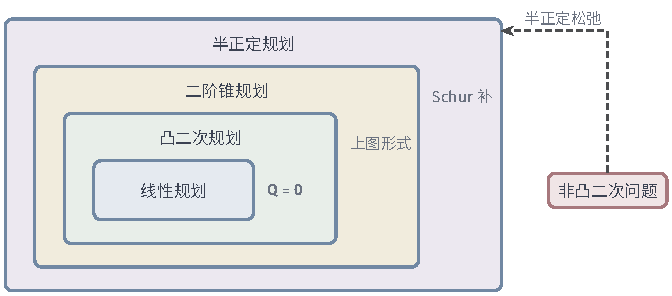
\includegraphics[width=112mm]{figures/05-optimization/06-constrained-optimization/tikz/cone-hierarchy/figure.pdf}
  \caption{模型的包含关系。边框旁标注内层写成外层所用的改写。非凸二次问题不在这条链上，它只能经半正定松弛（虚线）得到下界。}
  \label{fig:cone-hierarchy}
\end{BookInlineFigure}

这条链说的是表达能力，不是推荐的求解路线。外层的模型能表达内层的问题，但内层的结构在外层看不见了。一个$k+2$维的二阶锥写成线性矩阵不等式后，要用$(k+1)\times(k+1)$的矩阵，存储从$O(k)$变成$O(k^2)$。

内点法每步解一个线性方程，按稠密数据粗略估计：$n$个变量的二次规划，每步约$O(n^3)$次运算；变量为$n$、矩阵阶为$k$的线性矩阵不等式，组装牛顿方程的系数矩阵就要$O(nk^3+n^2k^2)$次，分解再要$O(n^3)$次\scite{math-boyd2004convex}。所以能用内层模型时就不要往外走。

\paragraph{松弛的规模}
半正定松弛的规模增长更快。问题~\eqref{eq:cone-sign-relax}把$n$个变量换成$n\times n$的矩阵。$n=1000$时，矩阵存储$10^6$个数，独立的非对角元有$n(n-1)/2=499500$个，一次特征分解约$10^9$次运算。此外还要重复取整和验证。松弛的结果换来的是一个下界，这个下界是否值得这样的代价，要看问题规模和对全局证据的需要。

\paragraph{各类方法的去向}
后面几章给出具体的算法，这里只说明各自处理什么情形。第~\ref{chap:sequential-quadratic-programming}章把二次规划当作子问题反复求解。第~\ref{chap:nonlinear-interior-point}章把第~\ref{chap:lp-interior-point}章的内点法推广到一般光滑约束和锥约束。

若可行集的投影便宜，或约束可以拆成几块分别处理，第~\ref{chap:feasible-iterations}章和第~\ref{chap:penalty-multiplier-methods}章的方法每步代价低得多，适合只需中等精度的大规模问题。

投影到半正定锥就是一个例子：作谱分解，把负特征值截成零。例如$\begin{bmatrix}1&2\\2&1\end{bmatrix}$的特征值是$3$和$-1$，特征向量是$(1,1)/\sqrt2$和$(1,-1)/\sqrt2$。截断负特征值后得到
\[
 3\cdot\frac12\begin{bmatrix}1&1\\1&1\end{bmatrix}=\frac32\begin{bmatrix}1&1\\1&1\end{bmatrix}.
\]
一次投影需要一次完整的特征分解，代价约$O(n^3)$，这决定了这类方法能处理的矩阵阶数。

\paragraph{选择的依据}
选择模型时可以按下面的顺序问。

\begin{enumerate}
 \item 问题是否凸？不凸的话，改写不会改变这一点，只能走局部方法或松弛。
 \item 能否停留在最内层的模型？线性约束的凸二次问题就用二次规划，不要因为通用求解器方便而升级。
 \item 数据有什么结构？稀疏、低秩或只能做矩阵向量积，决定是否可以分解，也决定内点法和一阶方法哪个更合算。
 \item 需要什么样的结论？只要一个好的解，局部方法足够；需要全局证据，就要付出松弛和对偶验证的代价。
\end{enumerate}

无论走哪条路，得到结果后都要分别核对，如图~\ref{fig:cone-workflow}所示。等价改写的解丢弃辅助变量后可以直接用，松弛的解则要先恢复再验证。

\begin{BookInlineFigure}
  \centering
  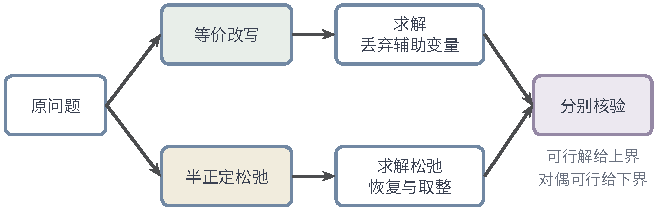
\includegraphics[width=110mm]{figures/05-optimization/06-constrained-optimization/tikz/cone-workflow/figure.pdf}
  \caption{从原问题到可靠结论的两条路径。等价改写（绿）保持最优解，求解后丢弃辅助变量。半正定松弛（黄）扩大可行集，求解后要恢复原变量。两条路径最后都要分别核验：可行解给出上界，对偶可行解给出下界。}
  \label{fig:cone-workflow}
\end{BookInlineFigure}

\section{本章小结}
\label{sec:cone-summary}

章首的三件事现在有了各自的归属。带预算的最小二乘是凸二次规划，距离上限的交集是二阶锥规划，相关系数的可行范围由半正定约束决定。把问题写成这些标准形式，是为了把目标的曲率、可行集的形状和可检验的对偶界摆到明面上。

二次规划要看的是$\bm{Q}$在可行差方向上的曲率，而不是全空间。这一曲率决定凸性和唯一性；凸时KKT条件是全局证书，非凸时KKT点可以是局部极小点或鞍点，证书不再成立。等式约束的情形化为线性方程，方程可逆只保证驻点唯一，极小性还要看约化Hessian。

锥规划把非负约束换成闭凸锥，乘子换成对偶锥的元素。弱对偶无条件成立，给出的下界可以直接验证；强对偶和最优解的达到则需要严格可行性等条件，线性规划的结论不能原样搬到半正定规划。

表~\ref{tab:cone-summary}比较后半章的两种操作。

\begin{BookInlineTable}
  \centering
  \begin{tabular}{lll}
    \toprule
    & 等价改写 & 半正定松弛\\
    \midrule
    可行集 & 投影后与原集合相同 & 严格扩大（一般情形）\\
    最优值 & 相等 & 不超过原最优值\\
    恢复原变量 & 丢弃辅助变量 & 秩一时直接读出，否则取整\\
    所需核对 & 改写的两个方向 & 可行性、对偶可行性、间隙\\
    典型工具 & 上图形式、Schur补 & 提升、删秩、随机取整\\
    \bottomrule
  \end{tabular}
  \caption{等价改写与半正定松弛的对比。}
  \label{tab:cone-summary}
\end{BookInlineTable}

算法返回的矩阵、原问题的可行解和最优性证书是三样不同的东西，需要分别检查。松弛最优矩阵不一定对应可行点，近似的原始值不是下界，只有经原约束核对的点给出上界，只有对偶可行的解给出下界，两者之差才是可以报告的结论。


\chapter{可行迭代}
\label{chap:feasible-iterations}

把一单位预算分给三个项目，$x_i$是第$i$个项目分到的比例。比例不能为负，三者之和必须为一，所以允许的分配构成一个三角形。假设方案的代价是下面的二次函数，三个系数表示各项目偏离理想份额时代价增长的快慢：
\begin{equation}
 f(\bm{x})=\frac12\Bigl[(x_1-1)^2+4\bigl(x_2-\tfrac58\bigr)^2+2x_3^2\Bigr].
 \label{eq:feas-running}
\end{equation}

理想份额$(1,\tfrac58,0)$的和是$\tfrac{13}{8}$，预算不够，所以约束一定起作用。梯度和Hessian分别是
\[
 \nabla f(\bm{x})=\bigl(x_1-1,\;4x_2-\tfrac52,\;2x_3\bigr),
 \qquad
 \nabla^2f=\operatorname{diag}(1,4,2).
\]
于是光滑常数$L=4$，强凸常数$\mu=1$。

这个问题的解是$\bm{x}^\star=(\tfrac12,\tfrac12,0)$，最优值$f^\star=\tfrac{5}{32}$，第~\ref{sec:feas-pgd-residual}节会验证这一点。图~\ref{fig:feas-running-simplex}把三维空间里的这个三角形摊平画出，三个顶点是把全部预算给一个项目的方案。解落在底边上，第三个项目分不到预算。

\begin{BookInlineFigure}
  \centering
  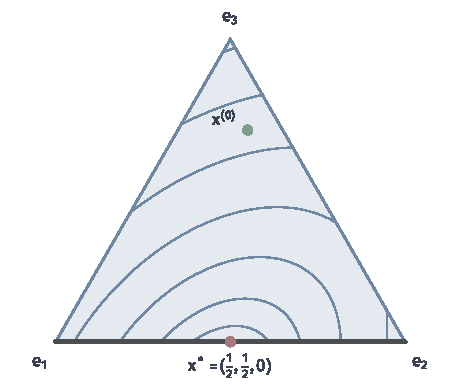
\includegraphics[width=78mm]{figures/05-optimization/06-constrained-optimization/matplotlib/feas-running-simplex/figure.pdf}
  \caption{贯穿全章的资源分配例。浅蓝三角形是$\{\bm{x}\geq\bm{0},\,x_1+x_2+x_3=1\}$，顶点$\bm{e}_i$是第$i$个坐标为$1$的单位向量。蓝线是式~\eqref{eq:feas-running}在三角形上的等高线，绿点是起点$(0.1,0.2,0.7)$，红点是最优解，深灰粗线是活动约束$x_3=0$所在的边。}
  \label{fig:feas-running-simplex}
\end{BookInlineFigure}

梯度下降的一步会把点带出三角形：坐标和不再是一，某些坐标可能变负。这一章研究的问题是：怎样让每个迭代点都满足原约束，保持可行又要付出多少计算？

第~\ref{sec:feas-updates}节先比较可以调用的几种运算。随后三节留在闭凸集合上，用同一个预算问题比较三种走法：先走再拉回最近点，朝线性模型的最优顶点靠拢，以及换一把更贴合比例结构的尺子。第~\ref{sec:feas-grg}节转向圆周这样的弯曲约束，这时连接两个可行点的线段不再可行，需要局部消元并解方程回到约束上。最后一节说明这些方法在什么前提下才能放在一起比较，以及算完之后应该报告什么。

\section{可行集合上的更新}
\label{sec:feas-updates}

设$\bm{C}\subseteq\mathbb{R}^n$是非空闭凸集，$f$在包含$\bm{C}$的开集上可微，要解
\begin{equation}
 \min_{\bm{x}\in\bm{C}}f(\bm{x}).
 \label{eq:feas-problem}
\end{equation}
有了当前可行点和它的梯度，还需要关于$\bm{C}$的什么额外运算，才能算出下一个可行点？

\paragraph{三种集合运算}
梯度只描述目标，对集合一无所知。把集合的信息送进更新，最常见的有三个渠道，它们分别回答三个不同的问题。

第一种是\term{投影}（projection）：给定任意点$\bm{z}$，问$\bm{C}$中离它最近的点在哪里。第二种是线性最小化：给定方向$\bm{g}$，问$\bm{C}$中沿$-\bm{g}$走得最远的点在哪里，也就是求$\min_{\bm{s}\in\bm{C}}\langle\bm{g},\bm{s}\rangle$。第三种是用一个由集合结构决定的非欧氏尺度求“最近点”，第~\ref{sec:feas-mirror}节会定义这把尺子。

图~\ref{fig:feas-three-oracles}在预算三角形上取同一个当前点，把三种运算画在一起。投影梯度先离开集合再回来，新点落在边界上；条件梯度沿当前点与顶点的线段移动，新点是两个可行点的组合；镜像更新走一条弯曲的路径，靠近边界时自动减速。

\begin{BookInlineFigure}
  \centering
  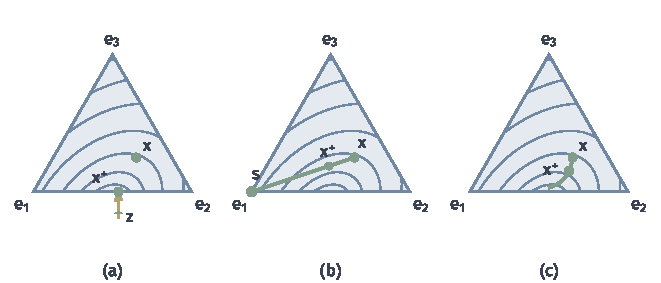
\includegraphics[width=112mm]{figures/05-optimization/06-constrained-optimization/matplotlib/feas-three-oracles/figure.pdf}
  \caption{预算三角形上从同一点$\bm{x}=(0.225,0.525,0.25)$出发的三种更新，为看清位移取较大的步长$\alpha=0.6$。(a)投影梯度：绿色箭头是平面内的梯度步，到达三角形外的空心点$\bm{z}$，黄色虚线把它拉回最近点$\bm{x}^{+}$。(b)条件梯度：线性模型在顶点$\bm{s}$处最优，新点是线段上的一点，图中取组合系数$0.25$。(c)镜像更新：绿线是步长从$0$增大时新点的轨迹，它始终留在三角形内部。}
  \label{fig:feas-three-oracles}
\end{BookInlineFigure}

\paragraph{凸性给了什么，没给什么}
$\bm{C}$凸意味着两个可行点之间的线段仍然可行。这保证条件梯度的组合可行，也保证投影存在唯一。图~\ref{fig:feas-segment-vs-curve}(a)画的就是这种情形。

凸性并不保证子问题便宜。在几千个一般线性不等式定义的多面体上，投影本身就是一个二次规划。在迹为一的半正定矩阵集合上，投影需要完整的特征分解，线性最小化却只需要一个最小特征向量。在单纯形上，投影和线性最小化都很便宜。所以选哪种方法，要先问手上的集合支持哪种运算。

\begin{BookInlineFigure}
  \centering
  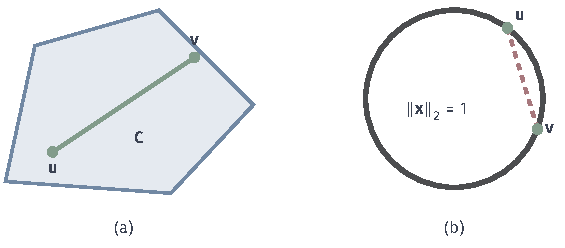
\includegraphics[width=95.75mm]{figures/05-optimization/06-constrained-optimization/tikz/feas-segment-vs-curve/figure.pdf}
  \caption{两种可行集合的差别。(a)凸集$\bm{C}$中两点$\bm{u},\bm{v}$的连线（绿色）留在集合内。(b)圆周$\lVert\bm{x}\rVert_2=1$上两点的连线（红色虚线）除端点外全部不可行，沿直线走的任何一步都要再回到圆周上。}
  \label{fig:feas-segment-vs-curve}
\end{BookInlineFigure}

\paragraph{各节使用的假设}
表~\ref{tab:feas-assumptions}列出后面各节的前提。前三行共用“集合是闭凸的”这一点，具体要求仍各不相同：条件梯度要求集合紧，否则线性子问题可能无解；镜像下降还要求势函数与集合匹配。

\begin{BookInlineTable}
  \centering
  \caption{本章各方法使用的集合、额外运算与评价量。}
  \label{tab:feas-assumptions}
  \begin{tabular}{llll}
   \toprule
   方法 & 集合 & 额外运算 & 评价量\\
   \midrule
   投影梯度 & 非空闭凸 & 欧氏投影 & 目标差、残差\\
   条件梯度 & 非空紧凸 & 线性最小化 & 目标差、间隙\\
   镜像下降 & 闭凸，配势函数 & Bregman子问题 & 平均点目标差\\
   GRG & 光滑等式加界 & 解方程 & 约束与KKT残差\\
   \bottomrule
  \end{tabular}
\end{BookInlineTable}

最后一行与前三行性质不同。图~\ref{fig:feas-segment-vs-curve}(b)的圆周不是凸集，前三种方法的保证都不能搬过去。第~\ref{sec:feas-grg}节依靠的是约束在当前点附近的局部可解性：Jacobian矩阵的一个方块要可逆，解非线性方程要能回到约束上。这些条件要逐点核对，它们失败的方式也和凸情形不同。

\section{投影梯度法（PGD）}
\label{sec:feas-pgd}

梯度步把点带出可行集合，能不能走完再拉回来，并且仍然保留梯度下降的保证？本节回答这个问题：先算投影，再说明残差应该怎样定义，最后证明下降和收敛。

\paragraph{主要思想}
回想第~\ref{chap:smooth-foundations}章的二次上界。在当前点$\bm{x}$，无约束的梯度步是在全空间最小化上界模型。现在只在$\bm{C}$上最小化同一个模型：
\[
 \bm{x}^{+}=\argmin_{\bm{y}\in\bm{C}}\Bigl\{f(\bm{x})+\langle\nabla f(\bm{x}),\bm{y}-\bm{x}\rangle+\frac{1}{2\alpha}\lVert\bm{y}-\bm{x}\rVert_2^2\Bigr\}.
\]

把花括号里关于$\bm{y}$的部分配方，常数项不影响最小点，得到
\[
 \bm{x}^{+}=\argmin_{\bm{y}\in\bm{C}}\frac{1}{2\alpha}\bigl\lVert\bm{y}-\bigl(\bm{x}-\alpha\nabla f(\bm{x})\bigr)\bigr\rVert_2^2.
\]
这正是求$\bm{C}$中离梯度步终点最近的点。

记$\bm{C}$上的欧氏投影为
\begin{equation}
 P_{\bm{C}}(\bm{z})=\argmin_{\bm{y}\in\bm{C}}\lVert\bm{y}-\bm{z}\rVert_2,
 \label{eq:feas-projection}
\end{equation}
\term{投影梯度法}（projected gradient descent，PGD）的迭代就是
\begin{equation}
 \bm{x}^{(t+1)}=P_{\bm{C}}\bigl(\bm{x}^{(t)}-\alpha^{(t)}\bm{g}^{(t)}\bigr).
 \label{eq:feas-pgd}
\end{equation}

第~\ref{chap:nonsmooth-composite-optimization}章把投影看作约束指标函数的邻近映射，这里复述要用到的三条结论。对非空闭凸集，投影存在且唯一；$\bm{p}=P_{\bm{C}}(\bm{z})$当且仅当$\bm{p}\in\bm{C}$且
\begin{equation}
 \langle\bm{z}-\bm{p},\bm{y}-\bm{p}\rangle\leq0,\quad\forall\bm{y}\in\bm{C};
 \label{eq:feas-projection-vi}
\end{equation}
投影不会拉大距离，也就是
\begin{equation}
 \lVert P_{\bm{C}}(\bm{u})-P_{\bm{C}}(\bm{v})\rVert_2\leq\lVert\bm{u}-\bm{v}\rVert_2.
 \label{eq:feas-nonexpansive}
\end{equation}

式~\eqref{eq:feas-projection-vi}有直观的几何含义：从$\bm{p}$看，$\bm{z}$和集合中任何一点的夹角都不小于直角。就像站在池塘边离某棵树最近的位置，整个池塘都在你身后的半边。

\subsection{投影计算}
\label{sec:feas-pgd-projection}

式~\eqref{eq:feas-pgd}的数学形式对所有闭凸集相同，能不能算则要看集合。本小节算出两个最常用的投影，并把预算例走几步。

\paragraph{盒约束}
设$\bm{C}=\{\bm{x}:\bm{l}\leq\bm{x}\leq\bm{u}\}$。目标$\sum_i(y_i-z_i)^2$和约束都按坐标分离，所以每个坐标单独处理：
\begin{equation}
 P_{\bm{C}}(\bm{z})_i=\min\bigl\{u_i,\max\{l_i,z_i\}\bigr\}.
 \label{eq:feas-box-projection}
\end{equation}
例如$\bm{C}=[0,1]^2$时，$(1.4,-0.3)$的投影是$(1,0)$。计算量是$O(n)$。

\paragraph{单纯形}
设$\bm{\Delta}$是$n$维概率单纯形：
\begin{equation}
 \bm{\Delta}=\{\bm{x}\in\mathbb{R}^n:\bm{x}\geq\bm{0},\ \bm{1}^\top\bm{x}=1\}.
 \label{eq:feas-simplex}
\end{equation}
坐标和的约束把各坐标绑在一起，不能逐坐标截断。写出投影子问题：
\[
 \min_{\bm{p}}\ \frac12\lVert\bm{p}-\bm{z}\rVert_2^2,
 \qquad
 \bm{1}^\top\bm{p}=1,\quad\bm{p}\geq\bm{0}.
\]
这是约束都为线性的凸问题，KKT条件既必要又充分，详见第~\ref{chap:constrained-optimality}章。

对等式引入乘子$\nu$，对$p_i\geq0$引入乘子$\lambda_i\geq0$，KKT条件是
\[
 p_i-z_i+\nu-\lambda_i=0,\qquad \lambda_ip_i=0.
\]

下面分两种情况。若$p_i>0$，则$\lambda_i=0$，于是$p_i=z_i-\nu$，这要求$z_i>\nu$。若$p_i=0$，则$\lambda_i=\nu-z_i\geq0$，这要求$z_i\leq\nu$。

两种情况合起来，所有坐标共用一个阈值$\nu$：
\begin{equation}
 p_i=\max\{z_i-\nu,0\},
 \qquad
 \varphi(\nu):=\sum_{i=1}^n\max\{z_i-\nu,0\}=1.
 \label{eq:feas-simplex-projection}
\end{equation}

$\varphi$连续、不增，在取正值的范围内严格递减，$\nu\to-\infty$时趋于无穷，$\nu$足够大时为零，所以方程$\varphi(\nu)=1$恰有一个解。

可以把$z_i$想成并排的水柱，$\nu$是一条水平刻度线，刻度线以上的部分就是分到的份额。把刻度线上下移动，直到露出部分的总量恰好是一。低于刻度线的项目一点也分不到。图~\ref{fig:feas-water-level}是这个图景。

\begin{BookInlineFigure}
  \centering
  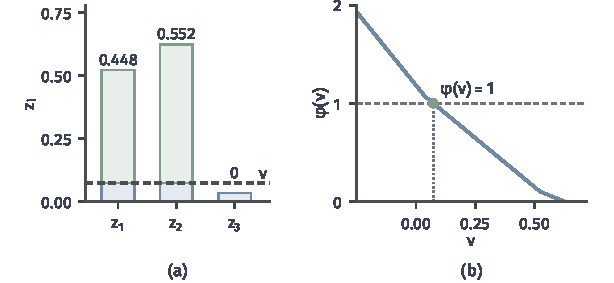
\includegraphics[width=104mm]{figures/05-optimization/06-constrained-optimization/matplotlib/feas-water-level/figure.pdf}
  \caption{单纯形投影的统一阈值，输入$\bm{z}=(0.521875,0.625,0.034375)$。(a)虚线是阈值$\nu$，绿色部分是投影结果，第三个柱子低于阈值，分到$0$。(b)$\varphi(\nu)$是分段线性的递减折线，在每个$z_i$处转折，绿点是$\varphi(\nu)=1$的解$\nu=0.0734375$。}
  \label{fig:feas-water-level}
\end{BookInlineFigure}

\paragraph{求阈值}
把$\bm{z}$从大到小排序为$z_{(1)}\geq\cdots\geq z_{(n)}$。若恰好前$k$个坐标取正，方程~\eqref{eq:feas-simplex-projection}给出
\[
 \nu_k=\frac{1}{k}\Bigl(\sum_{j=1}^kz_{(j)}-1\Bigr).
\]
正确的$k$是满足$z_{(k)}>\nu_k$的最大下标。计算量由排序决定，是$O(n\log n)$。

用图~\ref{fig:feas-water-level}的数据演示。先试$k=3$，$\nu_3=(1.18125-1)/3\approx0.0604$，而最小的坐标$0.034375<0.0604$，不满足要求。再试$k=2$：
\[
 \nu_2=\frac{0.521875+0.625-1}{2}=0.0734375.
\]
这次$z_{(2)}=0.521875>\nu_2$，所以$k=2$，投影是
\[
 \bm{p}=(0.4484375,\;0.5515625,\;0).
\]

\paragraph{投影不是归一化}
把$\bm{z}$除以坐标和也能得到和为一的向量，但这是另一个运算。取$\bm{z}=(0.325,0.625,0.35)$，坐标和$1.3$，归一化得到$(0.25,0.481,0.269)$；投影的阈值是$\nu=0.1$，结果是$(0.225,0.525,0.25)$。投影按相同的量减少各坐标，归一化按相同的比例缩小各坐标。

坐标有负值时差别更大。$\bm{z}'=(0.9,0.5,-0.4)$的坐标和恰好是一，归一化什么也不做，结果仍然不可行。投影取阈值$\nu=0.2$，得到$(0.7,0.3,0)$。图~\ref{fig:feas-projection-cases}(c)在两个坐标的情形画出这种差别：归一化沿过原点的射线回到直线，只有投影沿垂线回来。

\begin{BookInlineFigure}
  \centering
  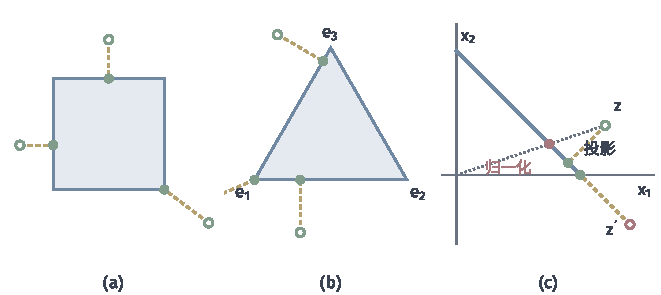
\includegraphics[width=112mm]{figures/05-optimization/06-constrained-optimization/matplotlib/feas-projection-cases/figure.pdf}
  \caption{投影的几何。空心点是输入，实心绿点是投影，黄色虚线是拉回的路径。(a)盒子$[0,1]^2$：逐坐标截断，右下方的点落在角上。(b)单纯形：输入点在三角形所在平面内，可能落到边上，也可能落到顶点。(c)两个坐标的单纯形（蓝线段）：$\bm{z}$的投影与归一化结果（红点，沿过原点的点线）不同；$\bm{z}'$的坐标和已为一，归一化不改变它，它仍然不可行，投影把它送到端点。}
  \label{fig:feas-projection-cases}
\end{BookInlineFigure}

\paragraph{昂贵的投影}
集合复杂时投影没有公式。在$\{\bm{x}:\bm{A}\bm{x}\leq\bm{b}\}$上，式~\eqref{eq:feas-projection}就是一个有$m$个不等式的二次规划，需要用第~\ref{chap:quadratic-conic-programming}章的算法迭代求解。这时外层每一步都包着一个内层优化，内层只能算到有限精度，第~\ref{sec:feas-pgd-step}节会讨论由此带来的误差。

\needspace{6\baselineskip}
\paragraph{变量}
\begin{itemize}
 \item $\bm{x}^{(t)}\in\bm{C}$：当前可行点。
 \item $\bm{g}^{(t)}\in\mathbb{R}^n$：当前梯度。
 \item $\bm{z}^{(t)}\in\mathbb{R}^n$：梯度步的终点，通常不可行。
 \item $\alpha>0$：步长；$\varepsilon>0$与$T$：容差与最大步数。
\end{itemize}

\paragraph{初始化}
取可行起点$\bm{x}^{(0)}\in\bm{C}$，步长$\alpha\leq1/L$，令$t=0$。例中用式~\eqref{eq:feas-running}，取$\alpha=1/L=1/4$，容差$\varepsilon=10^{-3}$，起点和目标值是
\[
 \bm{x}^{(0)}=(0.1,0.2,0.7),\qquad f(\bm{x}^{(0)})=1.25625.
\]

\needspace{6\baselineskip}
\paragraph{每轮更新}
在第$t$轮：
\begin{enumerate}
 \item \textbf{计算梯度步。}令$\bm{z}^{(t)}=\bm{x}^{(t)}-\alpha\bm{g}^{(t)}$。例中第一轮
 \[
  \bm{g}^{(0)}=(-0.9,-1.7,1.4),\qquad \bm{z}^{(0)}=(0.325,0.625,0.35).
 \]
 \item \textbf{投影。}由式~\eqref{eq:feas-simplex-projection}得$\bm{x}^{(t+1)}=P_{\bm{C}}(\bm{z}^{(t)})$。例中第一轮坐标和$1.3$，$k=3$，阈值$\nu=0.1$，于是
 \[
  \bm{x}^{(1)}=(0.225,0.525,0.25),\qquad f(\bm{x}^{(1)})\approx0.38281.
 \]
 \item \textbf{检查停止。}若相邻两点之差的长度除以$\alpha$不超过$\varepsilon$，或$t+1=T$，输出$\bm{x}^{(t+1)}$；否则$t\leftarrow t+1$。例中第一轮这个量约为$2.28$，继续。
\end{enumerate}

例中第二轮，$\bm{g}^{(1)}=(-0.775,-0.4,0.5)$，梯度步终点和投影依次是
\[
 \bm{z}^{(1)}=(0.41875,0.625,0.125),\qquad
 \bm{x}^{(2)}=(0.3625,0.56875,0.06875).
\]
这一轮$\nu=0.05625$，三个坐标仍然为正，$f(\bm{x}^{(2)})\approx0.21426$。

例中第三轮，$\bm{g}^{(2)}=(-0.6375,-0.225,0.1375)$，梯度步终点是图~\ref{fig:feas-water-level}用过的$\bm{z}^{(2)}$。前面已算出$\nu=0.0734375$，第三个坐标被截到零：
\[
 \bm{x}^{(3)}=(0.4484375,0.5515625,0),\qquad f(\bm{x}^{(3)})\approx0.16290.
\]

此后迭代留在底边上。由$x_3=0$和$x_2=1-x_1$代入，每轮的投影化成一维递推
\[
 x_1^{(t+1)}=\tfrac38x_1^{(t)}+\tfrac{5}{16},\qquad t\geq3,
\]
不动点是$x_1=\tfrac12$，误差每轮乘以$\tfrac38$。

第$10$轮的更新量降到容差以下，最终得到$\bm{x}^{(10)}\approx(0.49995,0.50005,0)$。图~\ref{fig:feas-pgd-path}(a)是这条路径，第三步落到活动边之后再也没有离开。

\begin{BookInlineFigure}
  \centering
  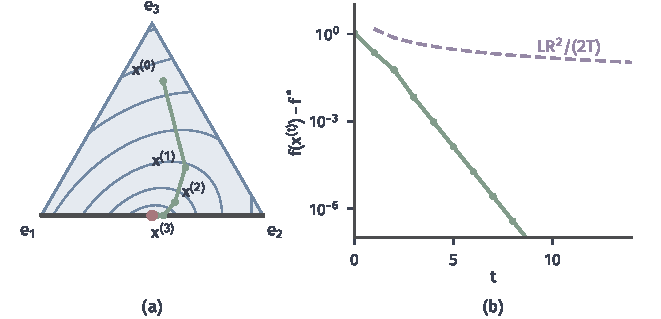
\includegraphics[width=112mm]{figures/05-optimization/06-constrained-optimization/matplotlib/feas-pgd-path/figure.pdf}
  \caption{预算例上的投影梯度法，$\alpha=1/4$，起点$(0.1,0.2,0.7)$。(a)绿色路径在第三步到达活动边（深灰），红点是最优解。(b)绿线是实际目标差，紫色虚线是第~\ref{sec:feas-pgd-step}节证明的上界$LR^2/(2T)$，$R^2=\lVert\bm{x}^{(0)}-\bm{x}^\star\rVert_2^2=0.74$。这个例子强凸，实际收敛比$1/T$快得多。}
  \label{fig:feas-pgd-path}
\end{BookInlineFigure}

\subsection{投影梯度残差}
\label{sec:feas-pgd-residual}

无约束时用$\lVert\nabla f\rVert_2$判断停止。有约束时这把尺子失灵：预算例的最优解处$\nabla f(\bm{x}^\star)=(-\tfrac12,-\tfrac12,0)$并不为零。那么应该用什么量来判断“已经到了”？

\paragraph{残差的定义}
一个点走不动，意思是走一步再投影又回到原地。把这个位移除以步长，单位就和梯度一致。

\begin{definition}[投影梯度残差]
\label{def:feas-residual}
设$\alpha>0$，$\bm{x}\in\bm{C}$。称
\begin{equation}
 \bm{G}_\alpha(\bm{x})=\frac{1}{\alpha}\Bigl[\bm{x}-P_{\bm{C}}\bigl(\bm{x}-\alpha\nabla f(\bm{x})\bigr)\Bigr]
 \label{eq:feas-residual}
\end{equation}
为\term{投影梯度残差}（projected gradient residual）。
\end{definition}

$\bm{C}=\mathbb{R}^n$时投影不起作用，$\bm{G}_\alpha=\nabla f$，所以它是梯度的推广。第~\ref{sec:feas-pgd-projection}节的停止量正是$\lVert\bm{G}_\alpha(\bm{x}^{(t)})\rVert_2$。

\paragraph{残差为零意味着什么}
凸集上的一阶必要条件是下面的\term{变分不等式}（variational inequality）：对可行方向$\bm{y}-\bm{x}$，目标的方向导数不能为负。推导很短：若$\bm{x}$是局部极小点，$\bm{y}\in\bm{C}$，线段$\bm{x}+s(\bm{y}-\bm{x})$在$s\in[0,1]$上可行，所以
\[
 0\leq\lim_{s\downarrow0}\frac{f(\bm{x}+s(\bm{y}-\bm{x}))-f(\bm{x})}{s}=\langle\nabla f(\bm{x}),\bm{y}-\bm{x}\rangle.
\]

\begin{theorem}[残差为零与变分不等式]
\label{thm:feas-residual}
设$\bm{C}$非空闭凸，$f$在$\bm{x}\in\bm{C}$处可微，$\alpha>0$。则$\bm{G}_\alpha(\bm{x})=\bm{0}$当且仅当
\begin{equation}
 \langle\nabla f(\bm{x}),\bm{y}-\bm{x}\rangle\geq0,\quad\forall\bm{y}\in\bm{C}.
 \label{eq:feas-vi}
\end{equation}
若$f$还是凸函数，这又等价于$\bm{x}$是$f$在$\bm{C}$上的全局最优解。
\end{theorem}

\begin{proof}
$\bm{G}_\alpha(\bm{x})=\bm{0}$就是$\bm{x}=P_{\bm{C}}(\bm{x}-\alpha\nabla f(\bm{x}))$。在式~\eqref{eq:feas-projection-vi}中取$\bm{p}=\bm{x}$，$\bm{z}=\bm{x}-\alpha\nabla f(\bm{x})$，这等价于
\[
 \langle-\alpha\nabla f(\bm{x}),\bm{y}-\bm{x}\rangle\leq0,\quad\forall\bm{y}\in\bm{C}.
\]
除以$-\alpha<0$，不等号反向，即得式~\eqref{eq:feas-vi}。

$f$凸时，切平面从下方托住目标，所以
\[
 f(\bm{y})\geq f(\bm{x})+\langle\nabla f(\bm{x}),\bm{y}-\bm{x}\rangle\geq f(\bm{x}),
\]
$\bm{x}$是全局最优解。反方向是前面的一阶必要条件。
\end{proof}

条件~\eqref{eq:feas-vi}里没有$\alpha$，所以残差对某一个$\alpha$为零，就对所有$\alpha>0$为零。残差的大小则随$\alpha$变化，比较时要固定步长。

\paragraph{边界最优点}
现在验证预算例的解。在$\bm{x}^\star=(\tfrac12,\tfrac12,0)$处，对任意$\bm{y}\in\bm{\Delta}$，利用$y_1+y_2=1-y_3$，得到
\[
 \langle\nabla f(\bm{x}^\star),\bm{y}-\bm{x}^\star\rangle
 =-\tfrac12(y_1+y_2)+\tfrac12
 =\tfrac12y_3\geq0.
\]
变分不等式成立，目标凸，所以$\bm{x}^\star$是全局最优解。把它代入式~\eqref{eq:feas-running}，得到
\[
 f^\star=\tfrac12\bigl[\tfrac14+\tfrac{1}{16}\bigr]=\tfrac{5}{32}.
\]

梯度不为零，但它指向的是“出不去”的方向。这就好比一个人靠墙站着，墙外地势更低：坡度不为零，他却走不动。图~\ref{fig:feas-boundary-residual}对比了两个边界点。最优点的梯度步终点垂直于活动边，投影原路拉回。另一个点的梯度步有沿边的分量，投影之后确实前进了。

\begin{BookInlineFigure}
  \centering
  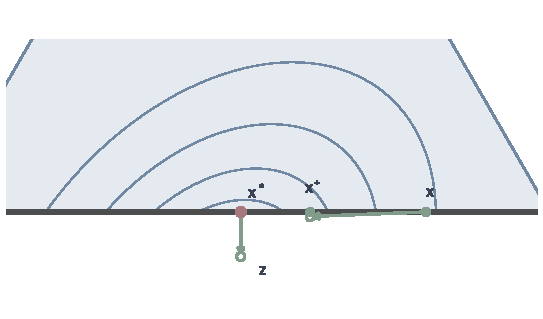
\includegraphics[width=92mm]{figures/05-optimization/06-constrained-optimization/matplotlib/feas-boundary-residual/figure.pdf}
  \caption{残差在活动边上的含义，局部放大底边，$\alpha=1/4$。红点$\bm{x}^\star$处，平面内的梯度步（绿色箭头）垂直离开边，投影回到原处，残差为零而梯度不为零。右侧的$\bm{x}=(0.2,0.8,0)$处，梯度步有沿边分量，投影后到达$\bm{x}^{+}$，残差不为零。}
  \label{fig:feas-boundary-residual}
\end{BookInlineFigure}

\paragraph{非凸时残差只检验驻定}
定理~\ref{thm:feas-residual}的后半句依赖凸性。取一元函数$f(x)=-x^2$，$\bm{C}=[-1,2]$。残差为零的点有三个：$x=-1$、$x=0$、$x=2$。

图~\ref{fig:feas-nonconvex-residual}画出了它们。$x=0$是目标的局部极大点；$x=-1$是约束上的局部极小点，$f=-1$；只有$x=2$是全局最优解，$f=-4$。残差只说明“在一阶意义下走不动”，不区分这三种情况。

\begin{BookInlineFigure}
  \centering
  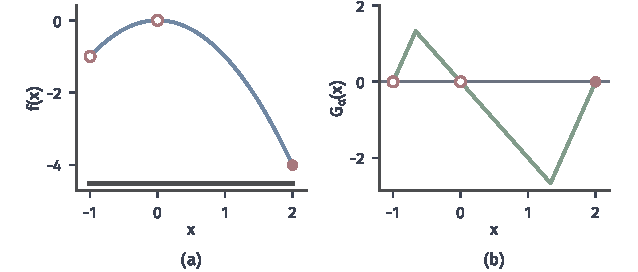
\includegraphics[width=108mm]{figures/05-optimization/06-constrained-optimization/matplotlib/feas-nonconvex-residual/figure.pdf}
  \caption{非凸目标$f(x)=-x^2$，$\bm{C}=[-1,2]$（深灰线）。(a)目标曲线，空心红点是局部极大点$0$和局部极小点$-1$，实心红点是全局最优解$2$。(b)$\alpha=1/4$时的残差$G_\alpha(x)$，在这三个点上都为零。}
  \label{fig:feas-nonconvex-residual}
\end{BookInlineFigure}

\subsection{步长与误差}
\label{sec:feas-pgd-step}

残差为零是目标。迭代是否真的把残差推向零，又需要什么步长？投影只能近似时，保证还剩多少？

\paragraph{单步下降}
投影性质~\eqref{eq:feas-projection-vi}告诉我们投影后的位移仍然是一个下降方向，这是下面所有结论的基础。

\begin{theorem}[投影梯度的单步下降]
\label{thm:feas-pgd-descent}
设$\bm{C}$非空闭凸，$f$在包含$\bm{C}$的开集上可微，且在$\bm{C}$上$L$光滑。对$\bm{x}\in\bm{C}$和$\alpha>0$，记$\bm{x}^{+}$是式~\eqref{eq:feas-pgd}的新点，有
\begin{equation}
 f(\bm{x}^{+})\leq f(\bm{x})-\alpha\Bigl(1-\frac{L\alpha}{2}\Bigr)\lVert\bm{G}_\alpha(\bm{x})\rVert_2^2.
 \label{eq:feas-pgd-descent}
\end{equation}
\end{theorem}

\begin{proof}
在式~\eqref{eq:feas-projection-vi}中取$\bm{z}=\bm{x}-\alpha\nabla f(\bm{x})$，$\bm{p}=\bm{x}^{+}$，$\bm{y}=\bm{x}$，得到
\[
 \langle\bm{x}-\alpha\nabla f(\bm{x})-\bm{x}^{+},\bm{x}-\bm{x}^{+}\rangle\leq0.
\]

整理后得到投影位移与梯度的内积：
\[
 \langle\nabla f(\bm{x}),\bm{x}^{+}-\bm{x}\rangle\leq-\frac1\alpha\lVert\bm{x}^{+}-\bm{x}\rVert_2^2.
\]

$\bm{C}$凸，线段$[\bm{x},\bm{x}^{+}]$在$\bm{C}$中，下降引理可用，于是
\[
 f(\bm{x}^{+})\leq f(\bm{x})+\langle\nabla f(\bm{x}),\bm{x}^{+}-\bm{x}\rangle+\frac L2\lVert\bm{x}^{+}-\bm{x}\rVert_2^2.
\]

把前一式代入，再用$\bm{x}^{+}-\bm{x}=-\alpha\bm{G}_\alpha(\bm{x})$，即得式~\eqref{eq:feas-pgd-descent}。
\end{proof}

只要$0<\alpha<2/L$，式~\eqref{eq:feas-pgd-descent}的括号就是正的，目标严格下降，除非已经驻定。这和无约束的下降估计形式完全相同，只是把梯度换成了残差。

\paragraph{非凸问题}
目标非凸时目标差无从谈起，能评价的是残差。这里需要目标在集合上有下界，否则下降可以无休止地进行。

\begin{theorem}[非凸情形的投影梯度]
\label{thm:feas-pgd-nonconvex}
在定理~\ref{thm:feas-pgd-descent}的条件下，设$f_{\inf}=\inf_{\bm{C}}f>-\infty$，取$\alpha=1/L$，则对$T\geq1$，
\begin{equation}
 \min_{0\leq t<T}\lVert\bm{G}_\alpha(\bm{x}^{(t)})\rVert_2^2\leq\frac{2L\bigl(f(\bm{x}^{(0)})-f_{\inf}\bigr)}{T},
 \label{eq:feas-pgd-nonconvex}
\end{equation}
并且$\{\bm{x}^{(t)}\}$的每个极限点都满足变分不等式~\eqref{eq:feas-vi}。
\end{theorem}

\begin{proof}
由式~\eqref{eq:feas-pgd-descent}，$\alpha=1/L$时
\[
 \frac{1}{2L}\lVert\bm{G}_\alpha(\bm{x}^{(t)})\rVert_2^2\leq f(\bm{x}^{(t)})-f(\bm{x}^{(t+1)}).
\]
对$t=0,\ldots,T-1$求和，右端裂项，并用$f(\bm{x}^{(T)})\geq f_{\inf}$，最小值不超过平均值，即得式~\eqref{eq:feas-pgd-nonconvex}。

级数$\sum_t\lVert\bm{G}_\alpha(\bm{x}^{(t)})\rVert_2^2$收敛，所以残差趋于零。若梯度连续，投影非扩张保证$\bm{G}_\alpha$连续，极限点处残差为零。定理~\ref{thm:feas-residual}给出结论。
\end{proof}

\paragraph{凸问题}
加上凸性和解的存在，可以用目标差衡量。证明的关键是把一步的目标差写成到解距离平方的差，这样求和时能够裂项。

\begin{theorem}[凸情形的投影梯度]
\label{thm:feas-pgd-convex}
在定理~\ref{thm:feas-pgd-descent}的条件下，设$f$在$\bm{C}$上凸，且存在最优解$\bm{x}^\star\in\bm{C}$，取$\alpha=1/L$。则对$T\geq1$，
\begin{equation}
 f(\bm{x}^{(T)})-f^\star\leq\frac{L\lVert\bm{x}^{(0)}-\bm{x}^\star\rVert_2^2}{2T}.
 \label{eq:feas-pgd-convex}
\end{equation}
若$f$还在$\bm{C}$上$\mu$强凸，$\mu>0$，则
\begin{equation}
 \lVert\bm{x}^{(t+1)}-\bm{x}^\star\rVert_2^2\leq\Bigl(1-\frac\mu L\Bigr)\lVert\bm{x}^{(t)}-\bm{x}^\star\rVert_2^2.
 \label{eq:feas-pgd-strong}
\end{equation}
\end{theorem}

\begin{proof}
记$\bm{x}=\bm{x}^{(t)}$，$\bm{x}^{+}=\bm{x}^{(t+1)}$，$\bm{g}=\nabla f(\bm{x})$，$\bm{y}\in\bm{C}$任取。由下降引理和$\mu$强凸的下界（$\mu=0$即凸），得到
\[
 \begin{aligned}
 f(\bm{x}^{+})&\leq f(\bm{x})+\langle\bm{g},\bm{x}^{+}-\bm{x}\rangle+\frac L2\lVert\bm{x}^{+}-\bm{x}\rVert_2^2,\\
 f(\bm{y})&\geq f(\bm{x})+\langle\bm{g},\bm{y}-\bm{x}\rangle+\frac\mu2\lVert\bm{y}-\bm{x}\rVert_2^2.
 \end{aligned}
\]

两式相减，消去$f(\bm{x})$：
\[
 f(\bm{x}^{+})-f(\bm{y})\leq\langle\bm{g},\bm{x}^{+}-\bm{y}\rangle+\frac L2\lVert\bm{x}^{+}-\bm{x}\rVert_2^2-\frac\mu2\lVert\bm{y}-\bm{x}\rVert_2^2.
\]

在式~\eqref{eq:feas-projection-vi}中取$\bm{z}=\bm{x}-\bm{g}/L$，$\bm{p}=\bm{x}^{+}$，整理得
\[
 \langle\bm{g},\bm{x}^{+}-\bm{y}\rangle\leq L\langle\bm{x}-\bm{x}^{+},\bm{x}^{+}-\bm{y}\rangle.
\]

再用恒等式展开$\lVert\bm{x}-\bm{y}\rVert_2^2$，它把内积化成三个距离平方：
\[
 2\langle\bm{x}-\bm{x}^{+},\bm{x}^{+}-\bm{y}\rangle
 =\lVert\bm{x}-\bm{y}\rVert_2^2-\lVert\bm{x}-\bm{x}^{+}\rVert_2^2-\lVert\bm{x}^{+}-\bm{y}\rVert_2^2.
\]

代回去，$\lVert\bm{x}^{+}-\bm{x}\rVert_2^2$的项抵消，得到
\[
 f(\bm{x}^{+})-f(\bm{y})\leq\frac{L-\mu}{2}\lVert\bm{x}-\bm{y}\rVert_2^2-\frac L2\lVert\bm{x}^{+}-\bm{y}\rVert_2^2.
\]

取$\bm{y}=\bm{x}^\star$，左端非负，移项除以$L/2$，就是式~\eqref{eq:feas-pgd-strong}；$\mu=0$时说明到解的距离不增。

$\mu=0$时对$t=0,\ldots,T-1$求和，右端裂项：
\[
 \sum_{t=1}^T\bigl(f(\bm{x}^{(t)})-f^\star\bigr)\leq\frac L2\lVert\bm{x}^{(0)}-\bm{x}^\star\rVert_2^2.
\]
由定理~\ref{thm:feas-pgd-descent}目标逐步下降，最后一项最小，不超过平均值，即得式~\eqref{eq:feas-pgd-convex}。
\end{proof}

预算例中$R^2=0.74$，$L=4$，上界是$1.48/T$，$T=1$时为$1.48$，实际目标差是$0.2266$。强凸的保证给出距离平方每步至少乘以$\tfrac34$。实际到达活动边之后因子是$(\tfrac38)^2\approx0.14$。约束把自由度减到一维，沿边方向$(1,-1,0)$的曲率是$\tfrac52$，比全空间最小的曲率$\mu=1$大。

\paragraph{$L$未知时}
可以用回溯代替固定步长：试探$\alpha$，算出$\bm{x}^{+}$，检查
\[
 f(\bm{x}^{+})\leq f(\bm{x})+\langle\nabla f(\bm{x}),\bm{x}^{+}-\bm{x}\rangle+\frac{1}{2\alpha}\lVert\bm{x}^{+}-\bm{x}\rVert_2^2,
\]
不满足就缩短$\alpha$。上面的证明只用到这个不等式，结论把$L$换成$1/\alpha_{\min}$仍成立。要注意，换一次$\alpha$就要重新投影，集合复杂时这是真实的成本。

\paragraph{近似投影}
投影由内层迭代求出时，输出$\tilde{\bm{x}}^{+}$与真投影有差距。设
\[
 \bigl\lVert\tilde{\bm{x}}^{+}-P_{\bm{C}}(\bm{x}-\alpha\nabla f(\bm{x}))\bigr\rVert_2\leq\varepsilon_t.
\]
这个误差有三种影响，要分别看待。

第一是可行性。输出到$\bm{C}$的距离不超过$\varepsilon_t$，但不一定是零，所以要单独检查原约束的残差。

第二是误差传播。设$f$的光滑、强凸条件在含所有迭代点的凸集上成立，定理~\ref{thm:feas-pgd-convex}说明精确映射把到解的距离至少缩小到$\rho=\sqrt{1-\mu/L}$倍。再加上三角不等式，得到
\begin{equation}
 \lVert\bm{x}^{(t+1)}-\bm{x}^\star\rVert_2\leq\rho\lVert\bm{x}^{(t)}-\bm{x}^\star\rVert_2+\varepsilon_t.
 \label{eq:feas-inexact-recursion}
\end{equation}

$\varepsilon_t\equiv\varepsilon$时展开递推，几何级数求和，距离的上极限不超过$\varepsilon/(1-\rho)$，迭代停在一个与内层精度成比例的范围里。没有强凸时$\rho=1$，上界只能写成$\lVert\bm{x}^{(0)}-\bm{x}^\star\rVert_2+\sum_t\varepsilon_t$，误差必须可求和才不累积。

第三是残差本身。用近似投影算出的残差$\tilde{\bm{G}}_\alpha$满足
\[
 \bigl\lvert\lVert\tilde{\bm{G}}_\alpha\rVert_2-\lVert\bm{G}_\alpha\rVert_2\bigr\rvert\leq\frac{\varepsilon_t}{\alpha}.
\]
所以步长越小，停止量受内层误差的污染越重。图~\ref{fig:feas-inexact-projection}显示了前两种影响。预算例中$\rho\approx0.866$，$1/(1-\rho)\approx7.46$。

\begin{BookInlineFigure}
  \centering
  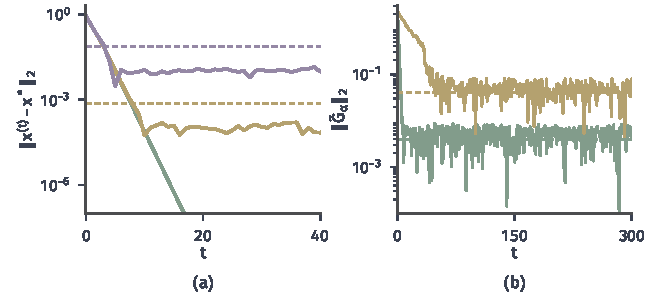
\includegraphics[width=112mm]{figures/05-optimization/06-constrained-optimization/matplotlib/feas-inexact-projection/figure.pdf}
  \caption{近似投影的影响，在每次投影结果上叠加固定种子的随机扰动，长度为$\varepsilon$。(a)到解的距离：绿线是精确投影，黄线$\varepsilon=10^{-4}$，紫线$\varepsilon=10^{-2}$，同色虚线是上界$\varepsilon/(1-\rho)$；距离停在上界之内。(b)$\varepsilon=10^{-3}$时算出的残差：绿线$\alpha=1/4$，黄线$\alpha=1/40$，同色虚线是$\varepsilon/\alpha$；步长小，平台反而高。}
  \label{fig:feas-inexact-projection}
\end{BookInlineFigure}

\paragraph{接近可行不等于接近最优}
内层把“输出离集合多远”算得很准，不能说明外层接近了解。预算例的顶点$\bm{e}_2=(0,1,0)$完全可行，可行误差为零，它的目标差却是$0.625$。可行性和最优性是两件事，都要报告。

\section{条件梯度法（Frank--Wolfe）}
\label{sec:feas-fw}

投影的代价可能很高，而同一个集合上的线性函数却容易最小化。能不能完全不做投影，只靠线性最小化来保持可行？本节回答这个问题：\term{条件梯度法}（conditional gradient method）也称\term{Frank--Wolfe法}（Frank--Wolfe method）\scite{frank1956algorithm}，它要求集合紧，用目标的一阶信息挑选集合的极点，再用凸组合保持可行。

\paragraph{主要思想}
把目标在当前点线性化，$f(\bm{x})+\langle\bm{g},\bm{s}-\bm{x}\rangle$。线性模型没有碗底，无约束时可以降到负无穷，这正是梯度下降要加二次项的原因。现在集合是紧的，线性模型在集合上有最小点，所以可以直接问：只信线性模型的话，集合里哪个点最好？

这个点$\bm{s}^{(t)}$通常在集合的远端，线性模型不能信到那么远。于是不跳过去，只沿连线走一段：
\begin{equation}
 \begin{aligned}
 \bm{s}^{(t)}&\in\argmin_{\bm{s}\in\bm{C}}\langle\bm{g}^{(t)},\bm{s}\rangle,\\
 \bm{x}^{(t+1)}&=\bm{x}^{(t)}+\alpha^{(t)}\bigl(\bm{s}^{(t)}-\bm{x}^{(t)}\bigr),\quad\alpha^{(t)}\in[0,1].
 \end{aligned}
 \label{eq:feas-fw}
\end{equation}

新点是两个可行点的凸组合，所以可行性由$\alpha^{(t)}\in[0,1]$和$\bm{C}$的凸性保证，不需要任何拉回操作。两种方法的次序相反：投影梯度先走一小步再修正，条件梯度先选定目标位置，再决定走多远。

\subsection{线性子问题}
\label{sec:feas-fw-linear}

式~\eqref{eq:feas-fw}的第一行要解一个线性规划。在单纯形上它有闭式解，并且解的形状决定了迭代点的结构。

\paragraph{单纯形上的线性最小化}
对任意$\bm{s}\in\bm{\Delta}$，$\bm{s}$的坐标非负且和为一，$\langle\bm{g},\bm{s}\rangle$是$g_i$的加权平均，所以
\[
 \langle\bm{g},\bm{s}\rangle=\sum_is_ig_i\geq\min_ig_i.
\]
等号在把全部权重放到最小坐标上时取得。因此线性子问题的一个解是顶点
\begin{equation}
 \bm{s}=\bm{e}_{i},\qquad i\in\argmin_kg_k.
 \label{eq:feas-simplex-lmo}
\end{equation}
只需找出梯度的最小分量，计算量是$O(n)$，不用排序。

这个结论在任何紧凸集上都有对应：线性函数的最小值总可以在极点处取到。所以线性子问题的解是集合中结构最简单的点。例如迹为一的半正定矩阵集合的极点是秩一矩阵，线性子问题的解就是$\bm{v}\bm{v}^\top$，其中$\bm{v}$是梯度矩阵最小特征值的单位特征向量。

\paragraph{稀疏表示}
每轮新点等于旧点乘以$1-\alpha^{(t)}$，再给选中的顶点加上权重$\alpha^{(t)}$。若把$\bm{x}^{(t)}$写成顶点的凸组合，权重的更新就是
\begin{equation}
 w_{v}\leftarrow(1-\alpha^{(t)})w_{v},\quad v\neq i;
 \qquad
 w_{i}\leftarrow(1-\alpha^{(t)})w_{i}+\alpha^{(t)}.
 \label{eq:feas-fw-weights}
\end{equation}

从一个顶点出发，每轮至多引入一个新顶点，所以$\bm{x}^{(t)}$至多是$t+1$个顶点的组合。在单纯形上这意味着至多有$t+1$个非零坐标。旧顶点的权重只被等比例缩小，这一点后面会成为问题。

\needspace{6\baselineskip}
\paragraph{变量}
\begin{itemize}
 \item $\bm{x}^{(t)}\in\bm{C}$：当前点；$\bm{g}^{(t)}$：当前梯度。
 \item $\bm{s}^{(t)}\in\bm{C}$：线性子问题的解，这里是顶点。
 \item $w_v$：各活跃顶点的权重，只在需要稀疏表示时保存。
 \item $\alpha^{(t)}\in[0,1]$：组合系数。
\end{itemize}

\paragraph{初始化}
选一个可行点，通常是一个顶点，令$t=0$。例中取$\bm{x}^{(0)}=\bm{e}_3=(0,0,1)$，目标值$f(\bm{x}^{(0)})=2.28125$，组合系数取预定序列
\begin{equation}
 \alpha^{(t)}=\frac{2}{t+2}.
 \label{eq:feas-fw-open-step}
\end{equation}

\needspace{6\baselineskip}
\paragraph{每轮更新}
在第$t$轮：
\begin{enumerate}
 \item \textbf{解线性子问题。}由式~\eqref{eq:feas-simplex-lmo}选顶点。例中第一轮
 \[
  \bm{g}^{(0)}=(-1,-2.5,2),\qquad \bm{s}^{(0)}=\bm{e}_2.
 \]
 \item \textbf{组合。}由式~\eqref{eq:feas-fw}计算新点。例中第一轮$\alpha^{(0)}=1$，新点直接跳到顶点，$\bm{e}_3$的权重变成零：
 \[
  \bm{x}^{(1)}=(0,1,0),\qquad f(\bm{x}^{(1)})=0.78125.
 \]
 \item \textbf{检查停止。}若$t+1=T$，输出$\bm{x}^{(t+1)}$；否则$t\leftarrow t+1$。第~\ref{sec:feas-fw-gap}节会给出可以计算的停止量，例中暂取$T=100$。
\end{enumerate}

例中第二轮，$\bm{g}^{(1)}=(-1,1.5,0)$，选$\bm{e}_1$，$\alpha^{(1)}=\tfrac23$，于是
\[
 \bm{x}^{(2)}=\bigl(\tfrac23,\tfrac13,0\bigr),\qquad f(\bm{x}^{(2)})\approx0.22569.
\]

例中第三轮，$\bm{g}^{(2)}=(-\tfrac13,-\tfrac76,0)$，选$\bm{e}_2$，$\alpha^{(2)}=\tfrac12$，于是
\[
 \bm{x}^{(3)}=\bigl(\tfrac13,\tfrac23,0\bigr),\qquad f(\bm{x}^{(3)})\approx0.22569.
\]

例中第四轮，$\bm{g}^{(3)}=(-\tfrac23,\tfrac16,0)$，选$\bm{e}_1$，$\alpha^{(3)}=\tfrac25$，于是
\[
 \bm{x}^{(4)}=\bigl(\tfrac35,\tfrac25,0\bigr),\qquad f(\bm{x}^{(4)})=0.18125.
\]

规律已经出现：两个顶点轮流被选中，迭代点在解$(\tfrac12,\tfrac12,0)$的两侧来回摆动，幅度慢慢变小。最终在$T=100$得到的点，目标差约为$6.1\times10^{-5}$。

图~\ref{fig:feas-fw-path-weights}画出路径和权重。第一步把起点的权重清零，这是$\alpha^{(0)}=1$的特殊效果。之后的权重在$\bm{e}_1$和$\bm{e}_2$之间来回转移。

\begin{BookInlineFigure}
  \centering
  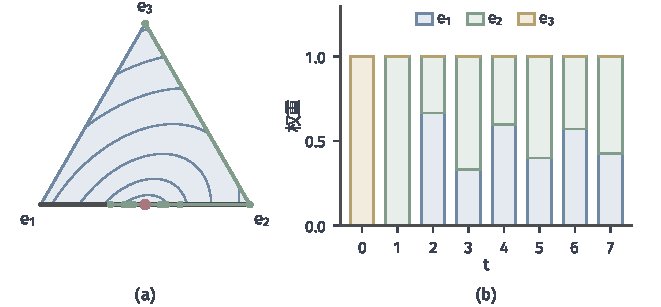
\includegraphics[width=112mm]{figures/05-optimization/06-constrained-optimization/matplotlib/feas-fw-path-weights/figure.pdf}
  \caption{条件梯度法的路径与权重，$\alpha^{(t)}=2/(t+2)$，从顶点$\bm{e}_3$出发。(a)绿色路径先跳到$\bm{e}_2$，然后沿活动边在解（红点）两侧摆动。(b)前$8$个迭代点在三个顶点上的权重，第$t$根柱子的三段高度是$\bm{x}^{(t)}$的三个坐标。}
  \label{fig:feas-fw-path-weights}
\end{BookInlineFigure}

\subsection{步长与可行性}
\label{sec:feas-fw-step}

式~\eqref{eq:feas-fw}中的$\alpha^{(t)}$可以怎样选，不同选法各用到什么信息？

\paragraph{三种规则}
记方向$\bm{d}^{(t)}=\bm{s}^{(t)}-\bm{x}^{(t)}$，用
\begin{equation}
 \Gamma^{(t)}=\langle\bm{g}^{(t)},\bm{x}^{(t)}-\bm{s}^{(t)}\rangle\geq0
 \label{eq:feas-fw-gamma-step}
\end{equation}
表示线性模型沿整条线段预测的下降量。三种规则如下。

\begin{itemize}
 \item \textbf{预定序列。}用式~\eqref{eq:feas-fw-open-step}，不需要函数值，也不需要$L$。
 \item \textbf{线搜索。}$\alpha^{(t)}\in\argmin_{\alpha\in[0,1]}f(\bm{x}^{(t)}+\alpha\bm{d}^{(t)})$，把范围限制在$[0,1]$是为了留在线段上。
 \item \textbf{光滑上界。}最小化下降引理的上界，在$[0,1]$上截断：
\end{itemize}
\begin{equation}
 \alpha^{(t)}=\min\Bigl\{1,\ \frac{\Gamma^{(t)}}{L\lVert\bm{d}^{(t)}\rVert_2^2}\Bigr\}.
 \label{eq:feas-fw-smooth-step}
\end{equation}

三种规则都使$\alpha^{(t)}\in[0,1]$。预定序列在$t\geq0$时取值从$1$递减。线搜索按定义在区间内。光滑上界的分子非负，分母为正（若分母为零，则$\bm{s}^{(t)}=\bm{x}^{(t)}$，已不必移动），再用$\min$截断。

在预算例的第一轮比较这三种规则。方向是$\bm{e}_2-\bm{e}_3=(0,1,-1)$，需要的几个量是
\[
 \Gamma^{(0)}=4.5,\qquad \lVert\bm{d}\rVert_2^2=2,\qquad \bm{d}^\top\bm{H}\bm{d}=6.
\]

二次目标上的精确线搜索是$\Gamma/(\bm{d}^\top\bm{H}\bm{d})$，所以
\[
 \alpha_{\text{预定}}=1,\qquad
 \alpha_{\text{线搜索}}=\tfrac34,\qquad
 \alpha_{\text{上界}}=\tfrac{9}{16}.
\]

对应的目标值分别是$0.78125$、$0.59375$和$0.69922$，图~\ref{fig:feas-fw-step-rules}(a)把这三点标在沿线段的目标曲线上。

\begin{BookInlineFigure}
  \centering
  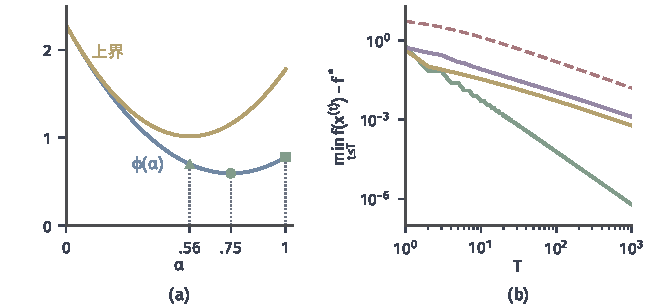
\includegraphics[width=112mm]{figures/05-optimization/06-constrained-optimization/matplotlib/feas-fw-step-rules/figure.pdf}
  \caption{组合系数的三种选法。(a)蓝线是从$\bm{e}_3$到$\bm{e}_2$的线段上的目标$\phi(\alpha)$，黄线是光滑上界，三角、圆点、方块分别是光滑上界、线搜索、预定序列对应的系数。(b)迄今最小目标差：绿线是预定序列，黄线是线搜索，紫线是光滑上界，红色虚线是定理~\ref{thm:feas-fw-rate}的上界$16/(T+2)$。}
  \label{fig:feas-fw-step-rules}
\end{BookInlineFigure}

\paragraph{有限步界}
下面证明目标差的上界，同时把线性子问题解得不准的情形放进去。设$\bm{C}$的直径是$D$，即集合中两点欧氏距离的最大值。证明要用到下一小节将要单独研究的一个事实，这里先在证明中直接用凸性得到。

\begin{theorem}[条件梯度法的有限步界]
\label{thm:feas-fw-rate}
设$\bm{C}$非空紧凸，直径为$D$，$f$在包含$\bm{C}$的开集上可微，在$\bm{C}$上凸且$L$光滑，$\delta\geq0$。设线性子问题的解$\tilde{\bm{s}}^{(t)}\in\bm{C}$满足
\begin{equation}
 \langle\bm{g}^{(t)},\tilde{\bm{s}}^{(t)}\rangle\leq\min_{\bm{s}\in\bm{C}}\langle\bm{g}^{(t)},\bm{s}\rangle+\frac{\delta}{2}\alpha^{(t)}LD^2,
 \label{eq:feas-inexact-lmo}
\end{equation}
并取$\alpha^{(t)}=2/(t+2)$。则对$T\geq1$，
\begin{equation}
 f(\bm{x}^{(T)})-f^\star\leq\frac{2(1+\delta)LD^2}{T+2}.
 \label{eq:feas-fw-rate}
\end{equation}
\end{theorem}

\begin{proof}
记$e_t=f(\bm{x}^{(t)})-f^\star$，$\alpha=\alpha^{(t)}$，$\bm{s}^\ast$是线性子问题的精确解。由下降引理，并用直径$D$放大移动的长度，得到
\[
 e_{t+1}\leq e_t+\alpha\langle\bm{g}^{(t)},\tilde{\bm{s}}^{(t)}-\bm{x}^{(t)}\rangle+\frac{L\alpha^2D^2}{2}.
\]

由式~\eqref{eq:feas-inexact-lmo}，把内积中的$\tilde{\bm{s}}^{(t)}$换成$\bm{s}^\ast$：
\[
 e_{t+1}\leq e_t+\alpha\langle\bm{g}^{(t)},\bm{s}^\ast-\bm{x}^{(t)}\rangle+\frac{(1+\delta)L\alpha^2D^2}{2}.
\]

由凸性，切平面在解处不高于目标，再由$\bm{s}^\ast$在线性模型上最优，得到
\[
 \langle\bm{g}^{(t)},\bm{s}^\ast-\bm{x}^{(t)}\rangle\leq\langle\bm{g}^{(t)},\bm{x}^\star-\bm{x}^{(t)}\rangle\leq-e_t.
\]

记$K=(1+\delta)LD^2$，于是得到递推
\[
 e_{t+1}\leq(1-\alpha^{(t)})e_t+\frac{K(\alpha^{(t)})^2}{2}.
\]

下面对$T$归纳证明$e_T\leq2K/(T+2)$。$t=0$时$\alpha^{(0)}=1$，递推给出$e_1\leq K/2\leq2K/3$。设$e_t\leq2K/(t+2)$，$t\geq1$，代入$\alpha^{(t)}=2/(t+2)$：
\[
 e_{t+1}\leq\frac{t}{t+2}\cdot\frac{2K}{t+2}+\frac{2K}{(t+2)^2}=\frac{2K(t+1)}{(t+2)^2}.
\]

由$(t+1)(t+3)\leq(t+2)^2$，右端不超过$2K/(t+3)$，归纳完成。
\end{proof}

$\delta$的作用是把内层误差与外层步长联系起来：式~\eqref{eq:feas-inexact-lmo}允许的误差随$\alpha^{(t)}$减小，也就是越到后面线性子问题要解得越准。如果误差固定不变，递推中多出常数项$\alpha^{(t)}\varepsilon$，目标差最终停在$\varepsilon$的量级。

线搜索和光滑上界的步长满足同样的上界。两者的新点都不高于在$\alpha=2/(t+2)$处的上界值，所以$\delta=0$时递推不变。第一轮的比较也说明，线搜索每步下降最多，并不代表后面的路径更好：图~\ref{fig:feas-fw-step-rules}(b)中，预定序列在这个例子上反而最快，第~\ref{sec:feas-fw-away}节解释其中的原因。

预算例中$D^2=2$，$L=4$，界~\eqref{eq:feas-fw-rate}是$16/(T+2)$，$T=100$时约为$0.157$，实际目标差约$6\times10^{-5}$。这个界对所有满足条件的问题都成立，所以偏于保守。线搜索的黄线大致按$1/T$下降：解在多面体的边上而不是顶点时，线搜索版本的目标差一般不能比$1/T$快多少，证明需要构造性的下界分析，篇幅较长，读者可查阅Frank--Wolfe方法收敛下界的专门文献。预定序列的绿线约按$1/T^2$下降，这来自两个顶点在解的两侧交替抵消的特殊结构，定理并不提供这样的保证。

\subsection{Frank--Wolfe间隙}
\label{sec:feas-fw-gap}

投影梯度用残差判断停止。条件梯度能不能在不知道$f^\star$的情况下，判断离最优还有多远？线性子问题已经算出了答案。

\paragraph{定义与上界}
式~\eqref{eq:feas-fw-gamma-step}的量可以对任意可行点定义。

\begin{definition}[Frank--Wolfe间隙]
\label{def:feas-fw-gap}
设$\bm{C}$非空紧凸，$f$在$\bm{x}\in\bm{C}$处可微，称
\begin{equation}
 \Gamma(\bm{x})=\max_{\bm{s}\in\bm{C}}\langle\nabla f(\bm{x}),\bm{x}-\bm{s}\rangle
 \label{eq:feas-fw-gap}
\end{equation}
为\term{Frank--Wolfe间隙}（Frank--Wolfe gap）。
\end{definition}

取$\bm{s}=\bm{x}$可知$\Gamma(\bm{x})\geq0$。它的值就是线性子问题的副产品，不需要额外计算：式~\eqref{eq:feas-fw-gamma-step}的$\Gamma^{(t)}$正是$\Gamma(\bm{x}^{(t)})$。

这里没有沿用字母$g$，因为$\bm{g}^{(t)}$已经表示梯度。

\begin{theorem}[间隙上界目标差]
\label{thm:feas-fw-gap}
在定义~\ref{def:feas-fw-gap}的条件下，$\Gamma(\bm{x})=0$当且仅当$\bm{x}$满足变分不等式~\eqref{eq:feas-vi}。若$f$在$\bm{C}$上凸，则
\begin{equation}
 f(\bm{x})-\min_{\bm{C}}f\leq\Gamma(\bm{x}).
 \label{eq:feas-fw-gap-bound}
\end{equation}
\end{theorem}

\begin{proof}
由式~\eqref{eq:feas-fw-gap}，$\Gamma(\bm{x})=0$就是对所有$\bm{s}\in\bm{C}$，$\langle\nabla f(\bm{x}),\bm{x}-\bm{s}\rangle\leq0$，这正是式~\eqref{eq:feas-vi}。

设$\bm{x}^\star$是最优解，它存在，因为$\bm{C}$紧、$f$连续。由凸性和$\Gamma$的定义，
\[
 f(\bm{x})-f(\bm{x}^\star)\leq\langle\nabla f(\bm{x}),\bm{x}-\bm{x}^\star\rangle\leq\Gamma(\bm{x}).
\]
\end{proof}

图~\ref{fig:feas-fw-gap-tangent}(a)在一元情形说明这个不等式。切线在集合上的最低值位于端点$\bm{s}$，凸函数高于切线，所以最优值高于切线的最低值。切线在当前点的高度是$f(\bm{x})$，$\Gamma$就是这段高度差。这和第~\ref{chap:duality}章用下界判断最优的思路相同，线性化给出了一个可计算的下界
\[
 f(\bm{x})-\Gamma(\bm{x})\leq f^\star.
\]

\begin{BookInlineFigure}
  \centering
  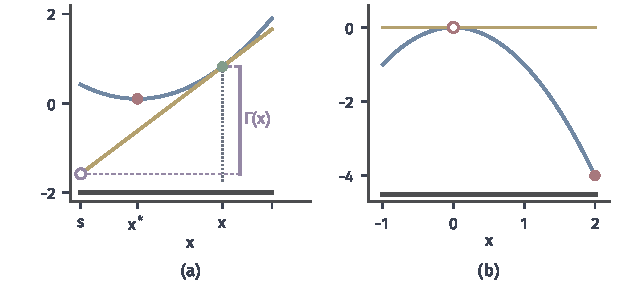
\includegraphics[width=108mm]{figures/05-optimization/06-constrained-optimization/matplotlib/feas-fw-gap-tangent/figure.pdf}
  \caption{间隙的几何。深灰线是可行区间，蓝线是目标，黄线是当前点的切线。(a)凸目标$f(x)=x^2/2+0.1$，$\bm{C}=[-0.8,1.9]$，$x=1.2$：切线在空心紫点处达到区间上的最低值，紫色线段的长度是$\Gamma(x)$，它不小于$f(x)-f^\star$。(b)非凸目标$-x^2$，$\bm{C}=[-1,2]$：局部极大点$x=0$处切线水平，$\Gamma=0$，而全局最优解在$2$。}
  \label{fig:feas-fw-gap-tangent}
\end{BookInlineFigure}

预算例中$\bm{x}^{(3)}=(\tfrac13,\tfrac23,0)$，梯度$(-\tfrac23,\tfrac16,0)$，最小分量是$-\tfrac23$，内积$\langle\bm{g},\bm{x}\rangle=-\tfrac{1}{9}$，于是
\[
 \Gamma(\bm{x}^{(3)})=-\tfrac19+\tfrac23=\tfrac59\approx0.556.
\]
真实目标差约为$0.0694$，不超过间隙。这说明了间隙的特点：可靠但往往偏大。图~\ref{fig:feas-fw-gap-curves}(a)的两条曲线一直保持这种上下关系。

用间隙做停止检验时，可以在每轮计算$\Gamma^{(t)}$，当它不超过容差时输出。把这一步放进第~\ref{sec:feas-fw-linear}节的每轮更新，就得到完整的算法。

\paragraph{非凸目标}
式~\eqref{eq:feas-fw-gap-bound}要用凸性。目标非凸时，$\Gamma=0$只表示一阶驻定，图~\ref{fig:feas-fw-gap-tangent}(b)的局部极大点就是例子。

不过间隙仍能作为进展的度量。取式~\eqref{eq:feas-fw-smooth-step}的步长，把$\lVert\bm{d}\rVert_2$放大为$D$，当$\Gamma\leq LD^2$时一步至少下降$\Gamma^2/(2LD^2)$，否则至少下降$\Gamma/2$。把这些下降量累加，并用$\Delta=f(\bm{x}^{(0)})-\inf_{\bm{C}}f$作为总额，得到
\begin{equation}
 \min_{0\leq t<T}\Gamma(\bm{x}^{(t)})\leq\max\Bigl\{\sqrt{\frac{2LD^2\Delta}{T}},\ \frac{2\Delta}{T}\Bigr\}.
 \label{eq:feas-fw-nonconvex}
\end{equation}
所以驻定度量以$1/\sqrt{T}$的速度减小，和投影残差~\eqref{eq:feas-pgd-nonconvex}开方之后的阶相同。

\paragraph{近似子问题的停止界}
当线性子问题只能近似求解时，设已知误差上界$\varepsilon$：
\[
 \langle\bm{g},\tilde{\bm{s}}\rangle\leq\min_{\bm{s}\in\bm{C}}\langle\bm{g},\bm{s}\rangle+\varepsilon.
\]
用近似解算出来的量记作
\[
 \tilde\Gamma=\langle\bm{g},\bm{x}-\tilde{\bm{s}}\rangle,
\]
它比真实间隙小。把定义和误差条件代入，得到
\begin{equation}
 \tilde\Gamma\leq\Gamma(\bm{x})\leq\tilde\Gamma+\varepsilon.
 \label{eq:feas-inexact-gap}
\end{equation}

$\tilde\Gamma$是真实间隙的下界，单用它停止可能过早。可靠的停止量是$\tilde\Gamma+\varepsilon$，所以必须知道内层求解误差的上界。图~\ref{fig:feas-fw-gap-curves}(b)让内层在最优顶点与次优顶点相差不超过$\varepsilon=0.1$时返回次优顶点，算出的$\tilde\Gamma$甚至可以是负数，而真实间隙一直夹在$\tilde\Gamma$与$\tilde\Gamma+\varepsilon$之间。

\begin{BookInlineFigure}
  \centering
  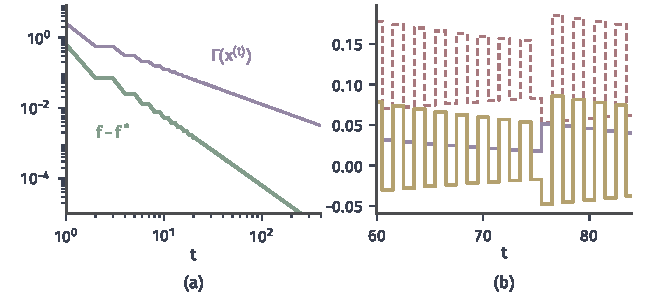
\includegraphics[width=112mm]{figures/05-optimization/06-constrained-optimization/matplotlib/feas-fw-gap-curves/figure.pdf}
  \caption{间隙作为证书，预算例，$\alpha^{(t)}=2/(t+2)$。(a)紫线是$\Gamma(\bm{x}^{(t)})$，绿线是目标差，前者始终在上方。(b)第$60$至$84$轮，内层返回次优顶点时：黄线是算出的$\tilde\Gamma$，紫线是真实间隙$\Gamma$，红色虚线是$\tilde\Gamma+\varepsilon$，$\varepsilon=0.1$。}
  \label{fig:feas-fw-gap-curves}
\end{BookInlineFigure}

\subsection{活跃顶点的调整（补充）}
\label{sec:feas-fw-away}

本小节是补充内容。第~\ref{sec:feas-fw-linear}节留下一个问题：旧顶点的权重只能等比例缩小。如果最优解不用某个顶点，这个顶点的权重永远消不掉，该怎么办？

\paragraph{之字形现象}
用精确线搜索从$\bm{e}_3$出发，第一步$\alpha=\tfrac34$，得到$(0,\tfrac34,\tfrac14)$。第二步$\alpha=\tfrac49$，得到$(\tfrac49,\tfrac{5}{12},\tfrac{5}{36})$。

$\bm{e}_3$的权重每步只乘以$1-\alpha^{(t)}$，线搜索的$\alpha^{(t)}$逐渐变小，第$1000$步第三个坐标仍约为$1.2\times10^{-3}$。图~\ref{fig:feas-fw-away}(a)显示，路径在底边上方反复横跳，既要减小$x_3$，又要调整$x_1,x_2$。这也解释了图~\ref{fig:feas-fw-step-rules}(b)：预定序列的第一步$\alpha^{(0)}=1$恰好把$\bm{e}_3$清零，这个好处只因为起点恰好是要丢弃的顶点，一般问题上不能指望。

\paragraph{远离步}
既然能朝好的顶点走，也应该能从坏的顶点离开。把$\bm{x}$写成活跃顶点集$\bm{S}$上的凸组合，权重$w_{\bm{v}}>0$。\term{远离步}（away step）选出活跃顶点中线性模型最差的一个，沿着背离它的方向走：
\begin{equation}
 \bm{v}^{(t)}\in\argmax_{\bm{v}\in\bm{S}}\langle\bm{g}^{(t)},\bm{v}\rangle,
 \qquad
 \bm{d}=\bm{x}^{(t)}-\bm{v}^{(t)}.
 \label{eq:feas-away}
\end{equation}

新点是$\bm{x}+\gamma\bm{d}$，各权重变成$(1+\gamma)w_{\bm{u}}$，而$\bm{v}^{(t)}$的权重变成$(1+\gamma)w_{\bm{v}}-\gamma$。它必须非负，这给出步长上限
\[
 \gamma\leq\gamma_{\max}=\frac{w_{\bm{v}}}{1-w_{\bm{v}}}.
\]
当$\bm{S}$只有一个顶点时$w_{\bm{v}}=1$，$\gamma_{\max}$无定义，这时不存在远离方向，只走普通的Frank--Wolfe步。取到$\gamma=\gamma_{\max}$时该顶点的权重正好变成零，从活跃集中删除，这称为丢弃步。

\paragraph{成对更新}
另一种做法是把权重直接从最差的活跃顶点搬到最好的顶点。\term{成对步}（pairwise step）取方向$\bm{d}=\bm{s}^{(t)}-\bm{v}^{(t)}$，权重更新是
\[
 w_{\bm{s}}\leftarrow w_{\bm{s}}+\gamma,\qquad
 w_{\bm{v}}\leftarrow w_{\bm{v}}-\gamma,\qquad
 0\leq\gamma\leq w_{\bm{v}}.
\]
其他权重不变，所有权重非负、和为一，所以新点仍是可行的凸组合。

用预算例走一遍，每步用精确线搜索并在上限处截断。第一步只有$\bm{e}_3$活跃，$\bm{s}=\bm{e}_2$，$\gamma=\tfrac34$，到达$(0,\tfrac34,\tfrac14)$。

第二步$\bm{g}=(-1,\tfrac12,\tfrac12)$，$\bm{s}=\bm{e}_1$，$\bm{e}_2,\bm{e}_3$并列最差，取$\bm{v}=\bm{e}_3$。方向$\bm{d}=(1,0,-1)$，精确步长是$1.5/3=\tfrac12$，超过上限$w_{\bm{e}_3}=\tfrac14$，于是截断成丢弃步：
\[
 \bm{x}=\bigl(\tfrac14,\tfrac34,0\bigr).
\]

第三步$\bm{g}=(-\tfrac34,\tfrac12,0)$，$\bm{s}=\bm{e}_1$，$\bm{v}=\bm{e}_2$，方向$(1,-1,0)$，精确步长$\tfrac{5/4}{5}=\tfrac14$，得到
\[
 \bm{x}=\bigl(\tfrac12,\tfrac12,0\bigr).
\]
三步到达最优解，此时$\Gamma=0$。图~\ref{fig:feas-fw-away}对比了这两条路径。

\begin{BookInlineFigure}
  \centering
  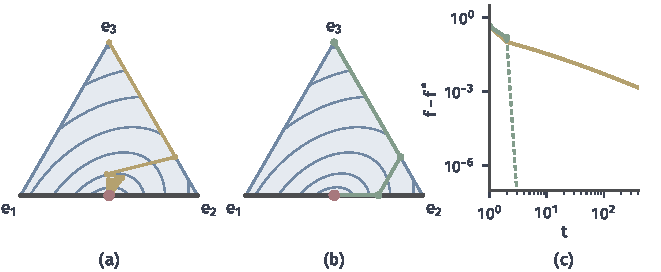
\includegraphics[width=112mm]{figures/05-optimization/06-constrained-optimization/matplotlib/feas-fw-away/figure.pdf}
  \caption{基本流程与成对更新，都用精确线搜索，从$\bm{e}_3$出发。(a)黄色路径是基本的条件梯度法，前$25$步在解上方横跳。(b)绿色路径是成对更新，第二步把$\bm{e}_3$的权重清零，第三步到达解。(c)目标差：黄线是基本流程，绿线是成对更新，第三步目标差为零，虚线表示落到坐标轴下方。}
  \label{fig:feas-fw-away}
\end{BookInlineFigure}

这个三维例子里，到达活动边后问题变成一维二次函数，线搜索一步到位，所以结果格外干净。不能由此推出删除顶点就有线性收敛。这类变体的线性收敛结论依赖目标的曲率、多面体的几何常数（描述顶点相对于面的“尖锐”程度），并要单独计数那些权重被顶到零的步，证明篇幅较长，读者可查阅关于Frank--Wolfe变体线性收敛的专门论文。此外，这些方法要保存活跃顶点及其权重，存储和维护的代价随活跃集增长。

\section{镜像下降}
\label{sec:feas-mirror}

在预算例中，把第三个项目的份额从$0.01$变到$0.02$和从$0.50$变到$0.51$，欧氏距离相同。可是前者把这个项目的份额翻了一倍，后者几乎没有变化。对比例这样的量，有没有一把更合适的尺子？本节回答这个问题：把投影梯度中的欧氏距离换成由凸势函数决定的代价，然后在单纯形上算出具体的公式。

\subsection{Bregman距离}
\label{sec:feas-bregman}

欧氏距离的平方可以看成是$\tfrac12\lVert\bm{x}\rVert_2^2$这个碗与它的切平面之间的高度差。换一只碗，就换了一把尺子。

\paragraph{定义}
设$h$是凸函数，在点$\bm{x}$可微。把$h$在$\bm{x}$处的切平面延伸到$\bm{u}$，势函数实际值高出切平面的量就是我们要的代价。

\begin{definition}[Bregman距离]
\label{def:feas-bregman}
设$h$是凸函数，在$\bm{x}$处可微，$\bm{u}\in\operatorname{dom}h$。称
\begin{equation}
 D_h(\bm{u},\bm{x})=h(\bm{u})-h(\bm{x})-\langle\nabla h(\bm{x}),\bm{u}-\bm{x}\rangle
 \label{eq:feas-bregman}
\end{equation}
为\term{势函数}$h$生成的\term{Bregman距离}（Bregman distance）。
\end{definition}

本节的$h$是势函数，与等式约束无关。由凸性，切平面不高于$h$，所以$D_h(\bm{u},\bm{x})\geq0$；若$h$严格凸，等号只在$\bm{u}=\bm{x}$时成立。

取$h(\bm{x})=\tfrac12\lVert\bm{x}\rVert_2^2$，代入式~\eqref{eq:feas-bregman}，得到
\[
 D_h(\bm{u},\bm{x})=\tfrac12\lVert\bm{u}\rVert_2^2-\tfrac12\lVert\bm{x}\rVert_2^2-\langle\bm{x},\bm{u}-\bm{x}\rangle=\tfrac12\lVert\bm{u}-\bm{x}\rVert_2^2.
\]
这时恰好是欧氏距离平方的一半。

\paragraph{不是真正的距离}
名字里虽有“距离”，$D_h$通常不对称，也不满足三角不等式。图~\ref{fig:feas-bregman-tangent}对比了两种势函数：抛物线上两条竖线段长度相等，$x\ln x$的曲线上两条竖线段长度不同。

\begin{BookInlineFigure}
  \centering
  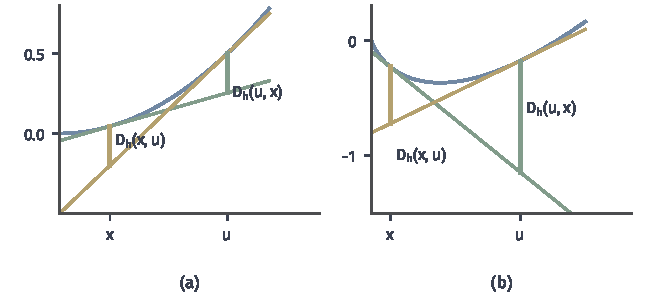
\includegraphics[width=112mm]{figures/05-optimization/06-constrained-optimization/matplotlib/feas-bregman-tangent/figure.pdf}
  \caption{Bregman距离是势函数高出切线的量。蓝线是势函数，绿线和黄线分别是$x$和$u$处的切线，同色竖线段分别是$D_h(u,x)$和$D_h(x,u)$。(a)$h(t)=t^2/2$，两段等长。(b)$h(t)=t\ln t$，$x=0.1$，$u=0.8$，两段不等长。}
  \label{fig:feas-bregman-tangent}
\end{BookInlineFigure}

用一个可手算的例子来看。取$h(\bm{x})=\sum_ix_i\ln x_i$和两个坐标和为一的点
\[
 \bm{u}=(0.5,0.5),\qquad\bm{x}=(0.2,0.8).
\]

这时$D_h(\bm{u},\bm{x})$就是$\sum_iu_i\ln(u_i/x_i)$，推导见第~\ref{sec:feas-entropy}节。代入两种顺序，得到
\[
 D_h(\bm{u},\bm{x})\approx0.2231,\qquad D_h(\bm{x},\bm{u})\approx0.1927.
\]

\paragraph{分析所需的条件}
把$D_h$用到算法里，有三件事要先核对。第一，$\nabla h(\bm{x})$必须存在，所以展开点要在$h$的可微区域内，对熵势就是相对内部。第二，要控制变量移动的大小，需要$h$在某个范数下强凸，也就是$D_h$能从下方控制这个范数的平方。第三，子问题要有解，这要看定义域与集合是否匹配。

图~\ref{fig:feas-kl-balls}比较了这把尺子的“单位球”。在三角形中央，熵势的球接近圆。靠近边界时，球在朝边界的方向被压扁：同样的代价只能让小坐标做很小的绝对变化。

\begin{BookInlineFigure}
  \centering
  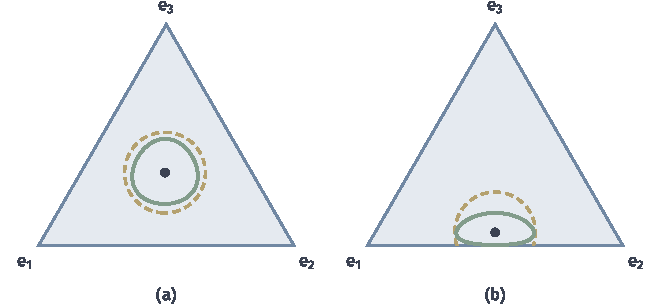
\includegraphics[width=112mm]{figures/05-optimization/06-constrained-optimization/matplotlib/feas-kl-balls/figure.pdf}
  \caption{同一单纯形上两把尺子的等距线。绿色实线是熵势的$\{\bm{u}:D_h(\bm{u},\bm{c})=0.05\}$，黄色虚线是欧氏圆$\{\bm{u}:\tfrac12\lVert\bm{u}-\bm{c}\rVert_2^2=0.025\}$，黑点是中心$\bm{c}$。(a)$\bm{c}\approx(1/3,1/3,1/3)$。(b)$\bm{c}=(0.47,0.47,0.06)$，靠近底边，绿色曲线在朝边的一侧被压扁，黄色圆已越出三角形。}
  \label{fig:feas-kl-balls}
\end{BookInlineFigure}

\subsection{镜像更新}
\label{sec:feas-mirror-update}

有了新尺子，更新公式是什么？它又如何退回熟悉的投影梯度？

\paragraph{主要思想}
投影梯度在$\bm{C}$上最小化线性模型加欧氏距离。把欧氏距离换成$D_h$，就得到\term{镜像下降法}（mirror descent）\scite{beck2003mirror}：
\begin{equation}
 \bm{x}^{(t+1)}\in\argmin_{\bm{x}\in\bm{C}}\Bigl\{\alpha^{(t)}\langle\bm{g}^{(t)},\bm{x}\rangle+D_h(\bm{x},\bm{x}^{(t)})\Bigr\}.
 \label{eq:feas-mirror}
\end{equation}
这里$\bm{g}^{(t)}$可以是当前梯度，也可以是目标非光滑时所选的一个凸次梯度。次梯度的定义见第~\ref{chap:nonsmooth-composite-optimization}章。

$D_h$的作用相当于一根弹簧，把新点拉住，不让它离当前点太远。不同的是，这根弹簧的松紧随位置变化。

\paragraph{完整的计算}
式~\eqref{eq:feas-mirror}可以拆成三步。设$\bm{C}$在$h$的可微区域内，先对$\bm{x}$求驻点。$D_h(\bm{x},\bm{x}^{(t)})$关于$\bm{x}$的梯度是$\nabla h(\bm{x})-\nabla h(\bm{x}^{(t)})$，于是无约束时的驻点$\bm{w}$满足
\begin{equation}
 \nabla h(\bm{w})=\nabla h(\bm{x}^{(t)})-\alpha^{(t)}\bm{g}^{(t)}.
 \label{eq:feas-mirror-dual}
\end{equation}

这说明梯度步不是在变量本身上走，而是在$\nabla h$的值上走。第一步，用$\nabla h$把$\bm{x}^{(t)}$映到梯度空间。第二步，在那里减去$\alpha^{(t)}\bm{g}^{(t)}$。第三步，用$\nabla h$的逆映射取回变量空间，得到$\bm{w}$。

$\bm{w}$可能不在$\bm{C}$中。把式~\eqref{eq:feas-mirror}的目标用式~\eqref{eq:feas-mirror-dual}改写，常数项不影响最小点，于是
\[
 \bm{x}^{(t+1)}=\argmin_{\bm{x}\in\bm{C}}D_h(\bm{x},\bm{w}).
\]
这是按$D_h$度量的投影。图~\ref{fig:feas-mirror-map}把这个往返过程画了出来，“镜像”这个名字指的就是$\nabla h$在两个空间之间的来回映射。

\begin{BookInlineFigure}
  \centering
  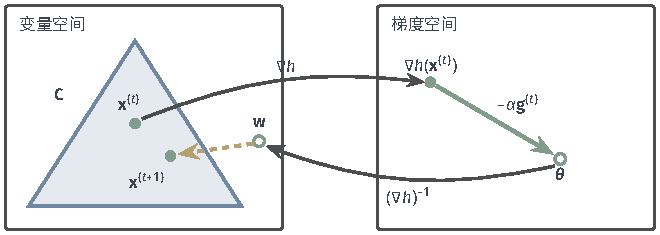
\includegraphics[width=111.74mm]{figures/05-optimization/06-constrained-optimization/tikz/feas-mirror-map/figure.pdf}
  \caption{镜像更新的结构。$\nabla h$把当前点送到梯度空间，绿色箭头在那里减去$\alpha\bm{g}^{(t)}$，逆映射把结果带回变量空间得到$\bm{w}$，黄色虚线按$D_h$投影回集合$\bm{C}$得到$\bm{x}^{(t+1)}$。}
  \label{fig:feas-mirror-map}
\end{BookInlineFigure}

取$h=\tfrac12\lVert\cdot\rVert_2^2$，$\nabla h$是恒等映射，式~\eqref{eq:feas-mirror-dual}给出$\bm{w}=\bm{x}^{(t)}-\alpha^{(t)}\bm{g}^{(t)}$，再做欧氏投影，正是式~\eqref{eq:feas-pgd}。所以投影梯度是镜像下降的特例。

\paragraph{其他势函数要核对的事}
换一个势函数，要分别回答三个问题。解是否存在：若$\bm{C}$紧、$h$连续，子问题有解；否则要检查水平集。解是否唯一：$h$严格凸时唯一。下一步能否继续：$\bm{x}^{(t+1)}$必须落在$h$的可微区域内，否则$\nabla h(\bm{x}^{(t+1)})$不存在，式~\eqref{eq:feas-bregman}无法展开。

第三个问题最容易被忽略。以一元势函数$h(x)=x^{3/2}$（定义域$x\geq0$）为例，导数$\tfrac32\sqrt{x}$在边界保持有限，梯度为正且步长足够大时，子问题的解就落在$x=0$上。这个点在定义域的边界，$h$作为定义域外取$+\infty$的函数在此处不可微。熵势不会发生这种事：它的导数在边界趋于$-\infty$，下一小节会看到迭代被挡在内部。

\subsection{熵势与指数更新}
\label{sec:feas-entropy}

单纯形上的比例变量适合用哪只碗？用\term{熵势}（entropic potential）可以把式~\eqref{eq:feas-mirror}解成闭式，并得到乘法形式的更新。

\paragraph{熵势}
取
\begin{equation}
 h(\bm{x})=\sum_{i=1}^nx_i\ln x_i,\qquad\bm{x}\geq\bm{0},
 \label{eq:feas-entropy}
\end{equation}
并按$0\ln0=0$延拓到坐标为零的边界。$h$在$\bm{x}\geq\bm{0}$上连续，梯度$\nabla h(\bm{x})_i=\ln x_i+1$只在所有坐标为正时存在，所以展开点必须是正向量。

对坐标和都为一的$\bm{u}$和正向量$\bm{x}$，代入式~\eqref{eq:feas-bregman}，线性项中的$\sum_i(u_i-x_i)$等于零，得到
\begin{equation}
 D_h(\bm{u},\bm{x})=\sum_{i=1}^nu_i\ln\frac{u_i}{x_i}.
 \label{eq:feas-kl}
\end{equation}

\paragraph{指数更新}
在$\bm{\Delta}$上解式~\eqref{eq:feas-mirror}。从正向量$\bm{x}^{(t)}$出发，暂时忽略$\bm{x}\geq\bm{0}$，只对等式约束引入乘子$\nu$，对$x_i$求偏导并令其为零：
\[
 \alpha g_i+\ln\frac{x_i}{x_i^{(t)}}+1+\nu=0.
\]

解出$x_i$，常数因子$\mathrm{e}^{-1-\nu}$对所有坐标相同，它由坐标和为一确定，于是
\begin{equation}
 x_i^{(t+1)}=\frac{x_i^{(t)}\exp\bigl(-\alpha g_i\bigr)}{\sum_{j=1}^nx_j^{(t)}\exp\bigl(-\alpha g_j\bigr)}.
 \label{eq:feas-exponential}
\end{equation}

结果每个坐标严格为正，所以被忽略的约束$\bm{x}\geq\bm{0}$确实不活跃，上面的驻点是原子问题的解（目标严格凸，驻点唯一）。下一步的展开点仍是正向量，迭代可以无限进行下去。这种\term{指数更新}（exponentiated update）是乘法的：梯度小的坐标放大，梯度大的坐标缩小，最后归一化。

\paragraph{两个坐标的比较}
设只有两个坐标，$\bm{x}=(0.9,0.1)$，$\bm{g}=(0,1)$，$\alpha=\tfrac12$。投影梯度的梯度步终点是$(0.9,-0.4)$，投影到线段上得到
\[
 \bm{x}^{+}_{\text{投影}}=(1,0).
\]

指数更新先算$(0.9,\;0.1\mathrm{e}^{-1/2})=(0.9,\;0.06065)$，归一化得
\[
 \bm{x}^{+}_{\text{镜像}}\approx(0.9369,0.0631).
\]
投影梯度一步把第二个坐标截到零，镜像更新只把它减小了约$37\%$。

两者的差别随坐标大小变化。两个坐标时投影更新是$x_2^{+}=\max\{x_2-\tfrac12\alpha(g_2-g_1),0\}$，变化量与$x_2$本身无关；镜像更新是乘以一个因子。图~\ref{fig:feas-exp-vs-proj}显示：$x_2=0.5$时两者起步斜率相同；$x_2=0.05$时投影很快归零，镜像更新则按比例缓慢减小。

\begin{BookInlineFigure}
  \centering
  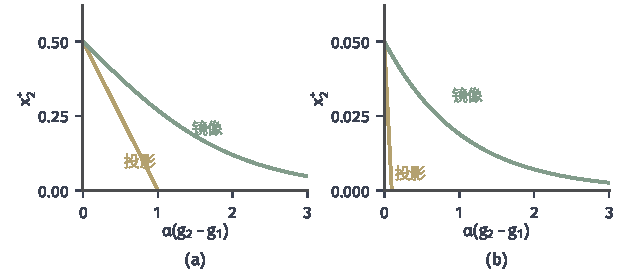
\includegraphics[width=108mm]{figures/05-optimization/06-constrained-optimization/matplotlib/feas-exp-vs-proj/figure.pdf}
  \caption{两个坐标的一步更新，横轴是梯度差乘步长，纵轴是新的$x_2$。黄线是投影更新，绿线是指数更新。(a)$x_2=0.5$，$x_2$较大时两者在起点相切。(b)$x_2=0.05$，投影在横轴$0.1$处归零，指数更新缓慢衰减。}
  \label{fig:feas-exp-vs-proj}
\end{BookInlineFigure}

\needspace{6\baselineskip}
\paragraph{变量}
\begin{itemize}
 \item $\bm{x}^{(t)}\in\bm{\Delta}$：当前点，所有坐标为正。
 \item $\bm{g}^{(t)}$：当前梯度或所选次梯度。
 \item $\bm{w}^{(t)}\in\mathbb{R}^n$：归一化前的正向量。
 \item $\alpha>0$：步长；$T$：总步数。
\end{itemize}

\paragraph{初始化}
取正向量起点，常用均匀分布。例中与投影梯度用同一起点$\bm{x}^{(0)}=(0.1,0.2,0.7)$，步长$\alpha=1/4$，第~\ref{sec:feas-mirror-progress}节说明这个步长的来历。

\needspace{6\baselineskip}
\paragraph{每轮更新}
在第$t$轮：
\begin{enumerate}
 \item \textbf{计算指数因子。}每个坐标乘以指数因子，得到$\bm{w}^{(t)}$。例中第一轮$\bm{g}^{(0)}=(-0.9,-1.7,1.4)$，于是
 \[
  \bm{w}^{(0)}\approx(0.12523,0.30592,0.49328).
 \]
 \item \textbf{归一化。}由式~\eqref{eq:feas-exponential}，把$\bm{w}^{(t)}$除以坐标和得到$\bm{x}^{(t+1)}$。例中第一轮分母约为$0.92443$，于是
 \[
  \bm{x}^{(1)}\approx(0.13547,0.33093,0.53361),\qquad f(\bm{x}^{(1)})\approx0.83140.
 \]
\end{enumerate}

例中第二轮$\bm{g}^{(1)}\approx(-0.8645,-1.1763,1.0672)$，分母约为$1.02087$，于是
\[
 \bm{x}^{(2)}\approx(0.16472,0.43499,0.40030),\qquad f(\bm{x}^{(2)})\approx0.58130.
\]

例中第三轮$\bm{g}^{(2)}\approx(-0.8353,-0.7601,0.8006)$，分母约为$1.05667$，于是
\[
 \bm{x}^{(3)}\approx(0.19208,0.49781,0.31011),\qquad f(\bm{x}^{(3)})\approx0.45489.
\]

运行到$T=60$，目标差约为$6.6\times10^{-5}$，第三个坐标始终为正。最终得到的$\bm{x}^{(60)}$在$x_3$上还有约$1.3\times10^{-4}$的残留量，它每轮大约乘以$0.88$，但不会精确到零。

图~\ref{fig:feas-md-path}将它和投影梯度比较。投影梯度在第$3$步把$x_3$截成零，之后活动集就固定了。镜像下降的路径光滑，$x_3$每轮大约乘以同一个因子。这是一种取舍：投影能识别出活动约束，镜像更新保持稠密的正权重。

\begin{BookInlineFigure}
  \centering
  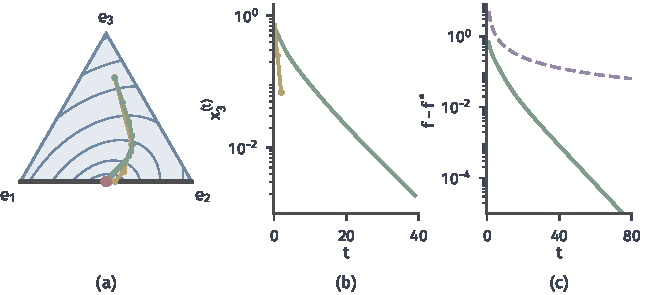
\includegraphics[width=112mm]{figures/05-optimization/06-constrained-optimization/matplotlib/feas-md-path/figure.pdf}
  \caption{预算例上的镜像下降（绿）与投影梯度（黄），步长都是$1/4$，起点$(0.1,0.2,0.7)$。(a)两条路径，镜像下降的路径弯曲着逼近底边。(b)第三个坐标$x_3^{(t)}$（对数轴）：投影梯度第$3$步起为零，从图中消失；镜像下降几何衰减。(c)镜像下降的目标差（绿）与定理~\ref{thm:feas-mirror-smooth}的上界$LD_h(\bm{x}^\star,\bm{x}^{(0)})/T$（紫色虚线）。}
  \label{fig:feas-md-path}
\end{BookInlineFigure}

\subsection{进展与输出}
\label{sec:feas-mirror-progress}

镜像下降的一次更新到底带来了多少进展？目标是否一定下降？答案取决于手上有哪种假设。

\paragraph{三点关系}
分析的工具是下面的引理，它把一次更新转成比较点到两个迭代点的$D_h$之差，求和时可以裂项。

\begin{lemma}[三点关系]
\label{lem:feas-three-point}
设$\bm{C}$闭凸，$h$在开集$\bm{U}$上可微且凸，$\bm{x}\in\bm{U}$，$\bm{x}^{+}$是式~\eqref{eq:feas-mirror}的解，并且$\bm{x}^{+}\in\bm{U}$。则对所有$\bm{u}\in\bm{C}\cap\operatorname{dom}h$，
\begin{equation}
 \alpha\langle\bm{g},\bm{x}^{+}-\bm{u}\rangle\leq D_h(\bm{u},\bm{x})-D_h(\bm{u},\bm{x}^{+})-D_h(\bm{x}^{+},\bm{x}).
 \label{eq:feas-three-point}
\end{equation}
\end{lemma}

\begin{proof}
式~\eqref{eq:feas-mirror}是凸目标在凸集上的最小化，$\bm{x}^{+}$满足变分不等式：
\[
 \bigl\langle\alpha\bm{g}+\nabla h(\bm{x}^{+})-\nabla h(\bm{x}),\ \bm{u}-\bm{x}^{+}\bigr\rangle\geq0.
\]

移项得到
\[
 \alpha\langle\bm{g},\bm{x}^{+}-\bm{u}\rangle\leq\bigl\langle\nabla h(\bm{x}^{+})-\nabla h(\bm{x}),\ \bm{u}-\bm{x}^{+}\bigr\rangle.
\]

把式~\eqref{eq:feas-bregman}的三个距离展开相减，$h(\bm{u})$、$h(\bm{x})$、$h(\bm{x}^{+})$都抵消，剩下的线性项正好是
\[
 D_h(\bm{u},\bm{x})-D_h(\bm{u},\bm{x}^{+})-D_h(\bm{x}^{+},\bm{x})
 =\bigl\langle\nabla h(\bm{x}^{+})-\nabla h(\bm{x}),\ \bm{u}-\bm{x}^{+}\bigr\rangle.
\]
代入上式即得结论。
\end{proof}

\paragraph{次梯度分析}
第一种情形只假设次梯度有界，目标可以不光滑。设$\lVert\cdot\rVert$是某个范数，它的对偶范数是
\[
 \lVert\bm{g}\rVert_{*}=\max_{\lVert\bm{v}\rVert\leq1}\langle\bm{g},\bm{v}\rangle.
\]

\begin{theorem}[镜像下降的平均点界]
\label{thm:feas-mirror-subgrad}
设$\bm{C}$闭凸，$f$在$\bm{C}$上凸，$\bm{g}^{(t)}$是$f$在$\bm{x}^{(t)}$处的次梯度，$\lVert\bm{g}^{(t)}\rVert_{*}\leq G$。设各迭代点都在$h$的可微区域内，且在$\bm{C}$上
\begin{equation}
 D_h(\bm{u},\bm{x})\geq\tfrac12\lVert\bm{u}-\bm{x}\rVert^2.
 \label{eq:feas-h-strong}
\end{equation}
取固定步长$\alpha$，平均点$\bar{\bm{x}}=\frac1T\sum_{t<T}\bm{x}^{(t)}$，则对$\bm{u}\in\bm{C}$，
\begin{equation}
 f(\bar{\bm{x}})-f(\bm{u})\leq\frac{D_h(\bm{u},\bm{x}^{(0)})}{\alpha T}+\frac{\alpha G^2}{2}.
 \label{eq:feas-mirror-rate}
\end{equation}
\end{theorem}

\begin{proof}
记$\bm{x}=\bm{x}^{(t)}$，$\bm{x}^{+}=\bm{x}^{(t+1)}$，$\bm{g}=\bm{g}^{(t)}$。由次梯度不等式，把内积拆成两部分：
\[
 \alpha\bigl(f(\bm{x})-f(\bm{u})\bigr)\leq\alpha\langle\bm{g},\bm{x}^{+}-\bm{u}\rangle+\alpha\langle\bm{g},\bm{x}-\bm{x}^{+}\rangle.
\]

第二项用对偶范数和Young不等式放大，再用$D_h$的强凸下界：
\[
 \alpha\langle\bm{g},\bm{x}-\bm{x}^{+}\rangle\leq\frac{\alpha^2G^2}{2}+\frac12\lVert\bm{x}-\bm{x}^{+}\rVert^2\leq\frac{\alpha^2G^2}{2}+D_h(\bm{x}^{+},\bm{x}).
\]

第一项用引理~\ref{lem:feas-three-point}，$D_h(\bm{x}^{+},\bm{x})$恰好抵消，得到
\[
 \alpha\bigl(f(\bm{x}^{(t)})-f(\bm{u})\bigr)\leq D_h(\bm{u},\bm{x}^{(t)})-D_h(\bm{u},\bm{x}^{(t+1)})+\frac{\alpha^2G^2}{2}.
\]

对$t=0,\ldots,T-1$求和，右端裂项，丢掉末项$D_h\geq0$。两边除以$\alpha T$，再用$f$的凸性把平均值换成$f(\bar{\bm{x}})$，即得结论。
\end{proof}

\paragraph{熵势给出的常数}
在单纯形上，取$\lVert\cdot\rVert=\lVert\cdot\rVert_1$，对偶范数是$\lVert\cdot\rVert_\infty$。熵势满足定理的强凸条件。设$\bm{v}=\bm{u}-\bm{x}$，$\bm{w}$是线段上任一点，$\nabla^2h(\bm{w})=\operatorname{diag}(1/w_i)$，由Cauchy--Schwarz不等式和$\sum_iw_i=1$，
\[
 \bm{v}^\top\nabla^2h(\bm{w})\bm{v}=\sum_i\frac{v_i^2}{w_i}\geq\frac{(\sum_i\lvert v_i\rvert)^2}{\sum_iw_i}=\lVert\bm{v}\rVert_1^2.
\]
由Taylor公式的积分余项，这给出式~\eqref{eq:feas-h-strong}，范数取$\lVert\cdot\rVert_1$。

从均匀分布出发，由式~\eqref{eq:feas-kl}和$\sum_iu_i\ln u_i\leq0$得到$D_h(\bm{u},\bm{x}^{(0)})\leq\ln n$。在式~\eqref{eq:feas-mirror-rate}中取$\alpha=\sqrt{2\ln n/T}/G$，得到
\begin{equation}
 f(\bar{\bm{x}})-f^\star\leq G\sqrt{\frac{2\ln n}{T}},\qquad\lVert\bm{g}^{(t)}\rVert_\infty\leq G.
 \label{eq:feas-entropy-rate}
\end{equation}

投影次梯度法对同一问题的上界要用$\lVert\bm{g}\rVert_2$，而$\lVert\bm{g}\rVert_2$可以大到$\sqrt{n}\,G$。所以梯度稠密时，熵势的上界在维数依赖上小了约$\sqrt{n/\ln n}$倍。这是两个上界的比较，并不保证熵势在每个问题上都更快。

\paragraph{光滑性带来的下降}
第二种情形假设$f$相对于$h$光滑，即存在$L>0$，使$Lh-f$在$\bm{C}$上凸。把凸性写成切平面不等式，它等价于
\begin{equation}
 f(\bm{u})\leq f(\bm{x})+\langle\nabla f(\bm{x}),\bm{u}-\bm{x}\rangle+LD_h(\bm{u},\bm{x}),
 \label{eq:feas-relative-smooth}
\end{equation}
称为\term{相对光滑}（relative smoothness）。$h=\tfrac12\lVert\cdot\rVert_2^2$时它就是下降引理。

预算例满足这个条件。单纯形上$x_i\leq1$，由此
\[
 \bm{v}^\top\nabla^2f\,\bm{v}\leq4\lVert\bm{v}\rVert_2^2\leq4\sum_i\frac{v_i^2}{x_i}=4\,\bm{v}^\top\nabla^2h\,\bm{v},
\]
所以$L=4$可用，这正是取$\alpha=1/4$的依据。

\begin{theorem}[相对光滑下的镜像下降]
\label{thm:feas-mirror-smooth}
设$f$凸可微，满足式~\eqref{eq:feas-relative-smooth}，各迭代点在$h$的可微区域内，取$\alpha=1/L$。则目标逐步下降，
\begin{equation}
 f(\bm{x}^{(t+1)})\leq f(\bm{x}^{(t)})-LD_h(\bm{x}^{(t)},\bm{x}^{(t+1)}),
 \label{eq:feas-mirror-descent}
\end{equation}
并且对$\bm{u}\in\bm{C}$，
\begin{equation}
 f(\bm{x}^{(T)})-f(\bm{u})\leq\frac{LD_h(\bm{u},\bm{x}^{(0)})}{T}.
 \label{eq:feas-mirror-smooth-rate}
\end{equation}
\end{theorem}

\begin{proof}
记$\bm{x}=\bm{x}^{(t)}$，$\bm{x}^{+}=\bm{x}^{(t+1)}$，$\bm{g}=\nabla f(\bm{x})$。由式~\eqref{eq:feas-relative-smooth}，
\[
 f(\bm{x}^{+})\leq f(\bm{x})+\langle\bm{g},\bm{x}^{+}-\bm{x}\rangle+LD_h(\bm{x}^{+},\bm{x}).
\]

在式~\eqref{eq:feas-three-point}中取$\alpha=1/L$，$\bm{u}=\bm{x}$，并用$D_h(\bm{x},\bm{x})=0$，得到
\[
 \langle\bm{g},\bm{x}^{+}-\bm{x}\rangle+LD_h(\bm{x}^{+},\bm{x})\leq-LD_h(\bm{x},\bm{x}^{+}).
\]
两式合起来就是下降式。

再用凸性给出的切平面下界$f(\bm{u})\geq f(\bm{x})+\cdots$，与上面第一式相减，得到
\[
 f(\bm{x}^{+})-f(\bm{u})\leq\langle\bm{g},\bm{x}^{+}-\bm{u}\rangle+LD_h(\bm{x}^{+},\bm{x}).
\]

用式~\eqref{eq:feas-three-point}，右端不超过$L\bigl[D_h(\bm{u},\bm{x})-D_h(\bm{u},\bm{x}^{+})\bigr]$。对$t$求和裂项，再由目标单调，最后一项不超过平均值，即得结论。
\end{proof}

预算例中$D_h(\bm{x}^\star,\bm{x}^{(0)})\approx1.263$，$L=4$，上界约为$5.05/T$，$T=60$时约为$0.084$，实际目标差约$6.6\times10^{-5}$。

\paragraph{目标不一定下降}
定理~\ref{thm:feas-mirror-subgrad}只保证平均点，不保证目标逐步下降，下面的例子说明这是真实的。在$\bm{\Delta}\subset\mathbb{R}^2$上取$f(\bm{x})=\lvert x_1-x_2\rvert$，$\bm{x}=(0.6,0.4)$，次梯度$\bm{g}=(1,-1)$，$\alpha=1$。由式~\eqref{eq:feas-exponential}，
\[
 \bm{x}^{+}\approx(0.1687,0.8313),\qquad f(\bm{x}^{+})\approx0.6626.
\]
目标从$0.2$升到了$0.6626$。次梯度步在不光滑的折点附近可以越过很远，所以输出时应使用平均点，或记录迄今最好的点。表~\ref{tab:feas-mirror-cases}对比了两种分析。

\begin{BookInlineTable}
  \centering
  \caption{镜像下降的两种分析。}
  \label{tab:feas-mirror-cases}
  \begin{tabular}{lll}
   \toprule
   & 次梯度分析 & 相对光滑分析\\
   \midrule
   目标 & 凸，可不光滑 & 凸，相对光滑\\
   势函数 & 按范数强凸 & $Lh-f$凸\\
   步长 & 依$T$或递减 & $1/L$\\
   目标值单调 & 否 & 是\\
   输出 & 平均点 & 最后一点\\
   上界的阶 & $1/\sqrt{T}$ & $1/T$\\
   \bottomrule
  \end{tabular}
\end{BookInlineTable}

\section{广义约化梯度法（GRG）}
\label{sec:feas-grg}

前三节都依赖集合的凸性。圆周$y^2+z^2=1$上，线段离开了约束，投影也不再有前面的性质。这时怎样从一个可行点走到另一个可行点？接下来要弄清：对光滑非线性约束，如何通过局部消元构造下降方向，又如何解方程回到约束上？

\paragraph{问题的形式}
考虑
\begin{equation}
 \min_{\bm{x}}f(\bm{x}),\qquad \bm{c}(\bm{x})=\bm{0},\quad \bm{l}\leq\bm{x}\leq\bm{u},
 \label{eq:feas-grg-problem}
\end{equation}
其中$\bm{c}:\mathbb{R}^n\to\mathbb{R}^p$连续可微，$p<n$。

不等式约束可以化成这个形式。对$g_i(\bm{x})\leq0$引入松弛变量$s_i$，改写成$g_i(\bm{x})+s_i=0$，$s_i\geq0$。例如$x_1^2+x_2^2\leq1$变成$x_1^2+x_2^2+s-1=0$，$s\geq0$。

\paragraph{主要思想}
$p$个方程把$n$个变量中的$p$个绑定了。选出$p$个变量让方程去决定，其余$n-p$个变量自由变动，约束问题就在局部变成只含自由变量的问题。这和线性规划单纯形法中“基变量由非基变量决定”的做法相同，只是这里方程非线性，决定关系是一条曲线，要靠隐函数定理保证存在，靠数值解方程求得。

\term{广义约化梯度法}（generalized reduced gradient method，GRG）依次做三件事：算自由变量上的下降方向，沿这个方向改变自由变量，再解方程把被绑定的变量拉回约束面。

\subsection{变量分块与局部消元}
\label{sec:feas-grg-partition}

选哪些变量由方程决定？选取时要满足什么条件，局部消元才成立？

\paragraph{分块}
把变量分成\term{基本变量}（basic variable）$\bm{y}\in\mathbb{R}^{p}$与\term{非基本变量}（nonbasic variable）$\bm{z}\in\mathbb{R}^{n-p}$，约束写成$\bm{c}(\bm{y},\bm{z})=\bm{0}$。对应地，把当前点的Jacobian矩阵按列分块，记
\begin{equation}
 \bm{B}=\frac{\partial\bm{c}}{\partial\bm{y}}\in\mathbb{R}^{p\times p},
 \qquad
 \bm{N}=\frac{\partial\bm{c}}{\partial\bm{z}}\in\mathbb{R}^{p\times(n-p)}.
 \label{eq:feas-grg-blocks}
\end{equation}

选择分块时有两条要求：$\bm{B}$可逆，基本变量严格位于上下界内。前者保证方程能确定$\bm{y}$，后者保证$\bm{y}$可以朝两边自由调整，用来补偿$\bm{z}$的变化。图~\ref{fig:feas-grg-partition}(a)是这种分块的示意。

\begin{BookInlineFigure}
  \centering
  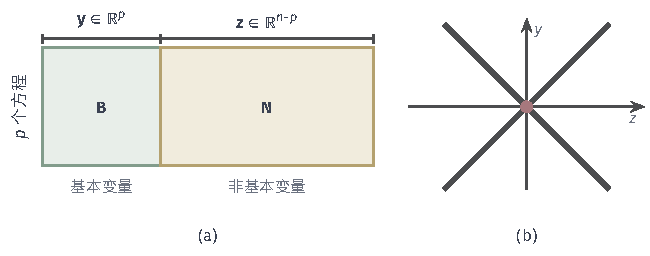
\includegraphics[width=110mm]{figures/05-optimization/06-constrained-optimization/tikz/feas-grg-partition/figure.pdf}
  \caption{局部消元的前提。(a)$p\times n$的Jacobian矩阵按变量分成可逆的方块$\bm{B}$（绿）和其余部分$\bm{N}$（黄）。(b)约束$y^2-z^2=0$的解集是两条相交直线，红点原点处的Jacobian矩阵为零，选哪个变量做基本变量都无法消元。}
  \label{fig:feas-grg-partition}
\end{BookInlineFigure}

\paragraph{局部解出基本变量}
隐函数定理说：若$\bm{c}$连续可微，$\bm{c}(\bm{y}_0,\bm{z}_0)=\bm{0}$，$\bm{B}$在该点可逆，则存在$\bm{z}_0$的邻域和其上唯一的连续可微函数$\bm{y}(\bm{z})$，满足$\bm{y}(\bm{z}_0)=\bm{y}_0$，$\bm{c}(\bm{y}(\bm{z}),\bm{z})=\bm{0}$。定理的证明可参考\BookChapterRef{chap:implicit-inverse-functions}{卷二第22章“隐函数与反函数”}。

把它代入目标，得到只含$\bm{z}$的\term{约化目标}（reduced objective）：
\begin{equation}
 F(\bm{z})=f\bigl(\bm{y}(\bm{z}),\bm{z}\bigr).
 \label{eq:feas-reduced-objective}
\end{equation}
$F$的定义只要求局部能解出$\bm{y}$，并不要求写出显式公式，也不要求全局成立。算法需要$\bm{y}(\bm{z})$的值时，就数值解一次方程。

\paragraph{例子}
本节用下面的问题贯穿：
\begin{equation}
 \min\ y,\qquad y^2+z^2=1.
 \label{eq:feas-circle}
\end{equation}
全局最优解是$(y,z)=(-1,0)$。在点$(\tfrac45,\tfrac35)$，取$y$为基本变量，$B=2y=\tfrac85$可逆，$N=2z=\tfrac65$。在这个点附近$y$由$z$决定，也就是圆周的上半弧：
\[
 y(z)=\sqrt{1-z^2},\qquad F(z)=\sqrt{1-z^2}.
\]
消元只在这一段弧上成立。到$z=\pm1$处$B=0$，上半弧到了头。

\paragraph{分块不存在的情形}
约束在某点的Jacobian矩阵行秩不足时，找不到可逆的$\bm{B}$。图~\ref{fig:feas-grg-partition}(b)的$y^2-z^2=0$在原点就是如此：解集是两条直线的交叉，附近根本不是某一个变量的函数。

基本变量都卡在界上也是一种退化：比如能使$\bm{B}$可逆的列组合都包含位于上下界的变量，这时$\bm{y}$没有双向调整的余地。这些情形需要另行处理，常用的办法有扰动、改用允许退化的换基规则，或换用第~\ref{chap:sequential-quadratic-programming}章的方法。

\subsection{约化梯度与下降方向}
\label{sec:feas-grg-gradient}

有了约化目标，它的梯度怎样算？能不能不必真正解出$\bm{y}(\bm{z})$？

\paragraph{推导}
沿约束面移动时，一阶变化$\mathrm{d}\bm{y}$和$\mathrm{d}\bm{z}$要让$\bm{c}$不变，所以
\[
 \bm{B}\,\mathrm{d}\bm{y}+\bm{N}\,\mathrm{d}\bm{z}=\bm{0}.
\]

解出基本变量的变化：
\begin{equation}
 \mathrm{d}\bm{y}=-\bm{B}^{-1}\bm{N}\,\mathrm{d}\bm{z}.
 \label{eq:feas-grg-dy}
\end{equation}

$\bm{z}$的改变不是孤立的，$\bm{y}$要跟着改变来补偿。目标的一阶变化是两部分之和：
\[
 \mathrm{d}F=\langle\nabla_{\bm{y}}f,\mathrm{d}\bm{y}\rangle+\langle\nabla_{\bm{z}}f,\mathrm{d}\bm{z}\rangle.
\]

代入式~\eqref{eq:feas-grg-dy}，把$\mathrm{d}\bm{z}$提出来，得到\term{约化梯度}（reduced gradient）：
\begin{equation}
 \nabla F=\nabla_{\bm{z}}f-\bm{N}^\top\bm{B}^{-\top}\nabla_{\bm{y}}f.
 \label{eq:feas-reduced-gradient}
\end{equation}

计算时不求逆。先解一个方阵方程$\bm{B}^\top\bm{\pi}=\nabla_{\bm{y}}f$，再算$\nabla F=\nabla_{\bm{z}}f-\bm{N}^\top\bm{\pi}$。$\bm{\pi}$是每单位约束变化的价格。线性约束、线性目标时，这个公式就是第~\ref{chap:simplex-method}章的约化成本。

\paragraph{圆周上的计算}
在式~\eqref{eq:feas-circle}中，$\nabla_yf=1$，$\nabla_zf=0$。在$(\tfrac45,\tfrac35)$，$B=\tfrac85$，$N=\tfrac65$，代入式~\eqref{eq:feas-reduced-gradient}：
\[
 \nabla F=0-\frac65\cdot\frac58\cdot1=-\frac34.
\]

用显式公式核对：$F'(z)=-z/\sqrt{1-z^2}$，在$z=\tfrac35$处正是$-\tfrac34$。

这个数的含义可以这样理解。目标本身不含$z$，$\nabla_zf=0$，单看目标似乎改变$z$没有用处。但$z$增加一点，约束的一阶变化要由$y$补偿：$\mathrm{d}y=-\tfrac34\mathrm{d}z$，而$y$就是目标。所以约化梯度记录的是“经过约束传导之后”的影响。图~\ref{fig:feas-grg-circle}画出了这个补偿三角形，以及约化目标的切线。

\begin{BookInlineFigure}
  \centering
  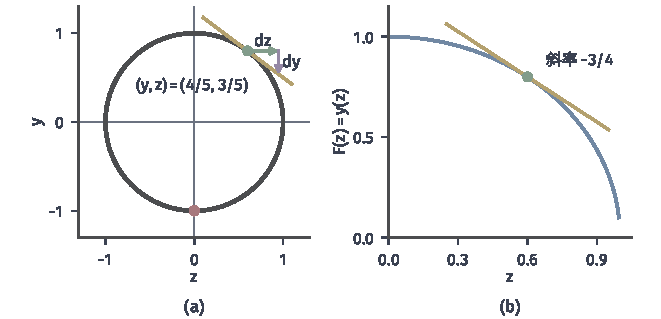
\includegraphics[width=112mm]{figures/05-optimization/06-constrained-optimization/matplotlib/feas-grg-circle/figure.pdf}
  \caption{圆周上的约化梯度。(a)深灰圆是约束，红点是最优解$(y,z)=(-1,0)$，绿点是当前点，黄线是切线；绿色箭头是$\mathrm{d}z$，紫色箭头是基本变量的一阶补偿$\mathrm{d}y=-\tfrac34\mathrm{d}z$。(b)约化目标$F(z)=\sqrt{1-z^2}$，在$z=3/5$处的切线斜率是$-3/4$。}
  \label{fig:feas-grg-circle}
\end{BookInlineFigure}

\paragraph{下降方向}
无界约束时可取$\bm{d}=-\nabla F$。非基本变量有上下界时，顶在界上又想继续往外走的坐标必须置零：
\begin{equation}
 d_j=\begin{cases}
 0,& z_j=l_j\text{ 且 }(\nabla F)_j>0,\\
 0,& z_j=u_j\text{ 且 }(\nabla F)_j<0,\\
 -(\nabla F)_j,& \text{其他}.
 \end{cases}
 \label{eq:feas-grg-direction}
\end{equation}

于是方向导数是
\[
 \langle\nabla F,\bm{d}\rangle=-\sum_{j:\,d_j\neq0}(\nabla F)_j^2.
\]
只要有一个未被置零的坐标，$\bm{d}$就是下降方向。

\subsection{可行恢复与线搜索}
\label{sec:feas-grg-restoration}

沿切向走一步之后点已经离开约束面。怎样回到约束面，又在哪里评价这一步的好坏？

\paragraph{主要思想}
固定候选的$\bm{z}^{+}=\bm{z}+\alpha\bm{d}$，把方程$\bm{c}(\bm{y},\bm{z}^{+})=\bm{0}$看成只含$\bm{y}$的$p$个方程，用Newton法求解，这个过程称为\term{可行恢复}（feasibility restoration）。切向预测$\bm{y}+\alpha\,\mathrm{d}\bm{y}$是一个已经算好的初值。

步长在恢复后的点上判断，比较$F(\bm{z}^{+})$，也就是真实可行点上的目标，而不是切线上的预测值。切线上的目标下降了，不等于回到约束面后依然下降。

\needspace{6\baselineskip}
\paragraph{变量}
\begin{itemize}
 \item $\bm{y}^{(t)}\in\mathbb{R}^p$，$\bm{z}^{(t)}\in\mathbb{R}^{n-p}$：当前基本变量与非基本变量，满足约束。
 \item $\bm{B},\bm{N}$：当前的Jacobian分块，见式~\eqref{eq:feas-grg-blocks}。
 \item $\bm{d}^{(t)}\in\mathbb{R}^{n-p}$：非基本变量的方向。
 \item $\alpha$：试探步长；$c_1\in(0,1)$：Armijo系数；$\varepsilon_c$：约束残差容差；$\varepsilon$：驻定容差。
\end{itemize}

\paragraph{初始化}
需要一个可行点和一个合格的分块。可行点本身可能要另解一个问题，例如最小化$\lVert\bm{c}(\bm{x})\rVert_2^2$。例中从式~\eqref{eq:feas-circle}的可行点出发，取$y$为基本变量，初始试探步长$\alpha=1/4$，$c_1=0.1$，$\varepsilon_c=10^{-10}$：
\[
 (y^{(0)},z^{(0)})=\bigl(\tfrac45,\tfrac35\bigr),\qquad F(z^{(0)})=0.8.
\]

\needspace{6\baselineskip}
\paragraph{每轮更新}
在第$t$轮：
\begin{enumerate}
 \item \textbf{算方向。}由式~\eqref{eq:feas-reduced-gradient}算约化梯度，由式~\eqref{eq:feas-grg-direction}得$\bm{d}^{(t)}$。若$\lVert\bm{d}^{(t)}\rVert_2\leq\varepsilon$，结束并进入第~\ref{sec:feas-grg-basis}节的检验。例中第一轮
 \[
  \nabla F=-0.75,\qquad d^{(0)}=0.75.
 \]

 \item \textbf{切向预测。}令$\bm{z}^{+}=\bm{z}^{(t)}+\alpha\bm{d}^{(t)}$，由式~\eqref{eq:feas-grg-dy}得初值
 \begin{equation}
  \bm{y}_0=\bm{y}^{(t)}-\bm{B}^{-1}\bm{N}\bigl(\bm{z}^{+}-\bm{z}^{(t)}\bigr).
  \label{eq:feas-grg-predict}
 \end{equation}
 例中第一轮
 \[
  z^{+}=0.7875,\qquad y_0=0.659375.
 \]

 \item \textbf{Newton恢复。}反复计算
 \begin{equation}
  \bm{y}_{k+1}=\bm{y}_k-\bm{B}(\bm{y}_k,\bm{z}^{+})^{-1}\bm{c}(\bm{y}_k,\bm{z}^{+}),
  \label{eq:feas-grg-newton}
 \end{equation}
 直到$\lVert\bm{c}\rVert_\infty\leq\varepsilon_c$。例中第一轮的各次结果是
 \[
  \begin{aligned}
  y_0&=0.659375, & c&=5.49\times10^{-2},\\
  y_1&=0.617721, & c&=1.74\times10^{-3},\\
  y_2&=0.616316, & c&=1.97\times10^{-6},\\
  y_3&=0.616315, & c&=2.56\times10^{-12}.
  \end{aligned}
 \]

 \item \textbf{在恢复点上做Armijo检验。}要求
 \[
  F(\bm{z}^{+})\leq F(\bm{z}^{(t)})+c_1\alpha\langle\nabla F,\bm{d}^{(t)}\rangle.
 \]
 通过就接受，否则把$\alpha$减半回到第2步。例中第一轮右端是$0.78594$，$F(z^{+})\approx0.61631$，接受。
\end{enumerate}

图~\ref{fig:feas-grg-recovery}(a)是这一轮的几何。切向预测点（空心）在圆外，Newton迭代沿竖直方向回到圆上。残差的下降呈二次收敛的样子。

\begin{BookInlineFigure}
  \centering
  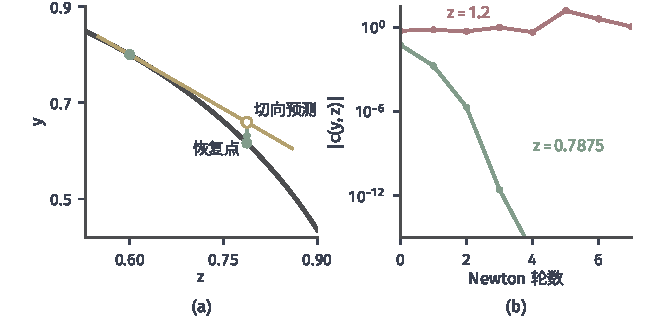
\includegraphics[width=112mm]{figures/05-optimization/06-constrained-optimization/matplotlib/feas-grg-recovery/figure.pdf}
  \caption{可行恢复。(a)从绿点沿切线（黄）走到空心点，固定$z=0.7875$后竖直回到圆周（深灰）。(b)Newton迭代中$\lvert c\rvert$的变化：绿线$z=0.7875$迅速收敛；红线$z=1.2$，方程$y^2+z^2=1$无实解，残差不减小。}
  \label{fig:feas-grg-recovery}
\end{BookInlineFigure}

例中第二轮从$(0.61632,0.7875)$出发，$\nabla F\approx-1.2778$，$d^{(1)}\approx1.2778$。先试$\alpha=\tfrac14$，得$z^{+}\approx1.1069$，超过了$1$，方程没有实解，Newton迭代的残差在几步内不降反升。

于是减半，$\alpha=\tfrac18$，$z^{+}\approx0.94722$，切向预测$y_0\approx0.41223$。Newton迭代依次给出$0.33077$、$0.32074$、$0.32059$，残差由$6.7\times10^{-2}$降到$2.5\times10^{-8}$，再一步达到容差。Armijo检验的右端约为$0.5959$，$F(z^{+})\approx0.32059$，接受：
\[
 (y^{(2)},z^{(2)})\approx(0.32059,0.94722).
\]

例中第三轮$\nabla F\approx-2.955$，方向更陡，而$z$离$1$只剩$0.053$。试探步长要连续减半四次到$\alpha=\tfrac{1}{64}$，得到$z^{+}\approx0.9934$，$y\approx0.1148$。此时$B=2y\approx0.23$已经很小，继续下去方程越来越病态，上半弧也快到头了。下一小节处理这个问题。

\paragraph{恢复失败时}
Newton迭代不收敛有几种可能的原因，处理也不同：步子太大，切向预测离约束面太远，办法是缩短$\alpha$；Jacobian矩阵过时，办法是重新计算；$\bm{B}$接近奇异，办法是换基。

恢复失败和原问题无可行解是两回事。第二轮的$z=1.1069$处方程无解，可是当前点$(0.61632,0.7875)$本身可行。恢复失败只说明这个候选的$\bm{z}^{+}$在这个分块下没有对应的可行点。

\paragraph{恢复容差与Jacobian更新}
恢复的容差要按原约束残差$\lVert\bm{c}\rVert_\infty$设置，不能按Newton步的长度设置。步长短不等于残差小，$\bm{B}$病态时尤其如此。

为了省计算，实现中常常冻结$\bm{B}$，每次Newton迭代只重新算残差。这样收敛变成线性的。第一轮冻结$B=1.6$时，残差依次是
\[
 5.49\times10^{-2},\quad1.08\times10^{-2},\quad2.42\times10^{-3},\quad5.51\times10^{-4},
\]
每次大约缩小$4.5$倍。省下分解矩阵的钱，要用更多的残差计算来付。残差下降变慢时就该更新$\bm{B}$。

\subsection{界约束与换基}
\label{sec:feas-grg-basis}

上面的例子留下两个问题：分块何时必须更换？算法停下来时，怎样判断这个点满足原问题的最优性条件？

\paragraph{一阶必要性}
第~\ref{chap:constrained-optimality}章的KKT条件要求：存在等式乘子和上下界乘子$\bm{\lambda}^{l},\bm{\lambda}^{u}\geq\bm{0}$，使Lagrange函数的梯度为零，并满足互补条件。对问题~\eqref{eq:feas-grg-problem}，这个条件可以用约化梯度来检验。

\begin{theorem}[约化梯度与KKT条件]
\label{thm:feas-grg-kkt}
设$\bm{x}=(\bm{y},\bm{z})$满足式~\eqref{eq:feas-grg-problem}的约束，$\bm{B}$可逆，$\bm{l}_{\bm{y}}<\bm{y}<\bm{u}_{\bm{y}}$。则$\bm{x}$满足KKT条件，当且仅当约化梯度~\eqref{eq:feas-reduced-gradient}的每个分量满足
\begin{equation}
 (\nabla F)_j\begin{cases}
 \geq0,& z_j=l_j,\\
 \leq0,& z_j=u_j,\\
 =0,& l_j<z_j<u_j.
 \end{cases}
 \label{eq:feas-grg-signs}
\end{equation}
此时等式乘子是$\bm{\nu}=-\bm{B}^{-\top}\nabla_{\bm{y}}f$。
\end{theorem}

\begin{proof}
KKT条件的驻定部分按两组变量写开。基本变量严格在界内，互补性使它们的上下界乘子为零，所以
\[
 \nabla_{\bm{y}}f+\bm{B}^\top\bm{\nu}=\bm{0}.
\]
$\bm{B}$可逆，这唯一地确定$\bm{\nu}=-\bm{B}^{-\top}\nabla_{\bm{y}}f$。

非基本变量的驻定条件是
\[
 \nabla_{\bm{z}}f+\bm{N}^\top\bm{\nu}-\bm{\lambda}^{l}_{\bm{z}}+\bm{\lambda}^{u}_{\bm{z}}=\bm{0}.
\]

把$\bm{\nu}$代入，前两项之和正是$\nabla F$，于是
\[
 \nabla F=\bm{\lambda}^{l}_{\bm{z}}-\bm{\lambda}^{u}_{\bm{z}}.
\]

由互补性，$z_j=l_j$时$\lambda^u_j=0$，$(\nabla F)_j=\lambda^l_j\geq0$；$z_j=u_j$时$(\nabla F)_j=-\lambda^u_j\leq0$；在界内时两个乘子都是零，$(\nabla F)_j=0$。反过来，满足式~\eqref{eq:feas-grg-signs}时，按这三种情况取乘子就得到KKT条件。
\end{proof}

用圆周例检验。加上界$z\leq\tfrac35$，点$(\tfrac45,\tfrac35)$处非基本变量在上界，$\nabla F=-\tfrac34\leq0$，符号条件成立。此时$\nu=-\tfrac58$，上界乘子是$\tfrac34$，这个点是带界问题的最优解。若没有这个上界，$\nabla F\neq0$，它就不是驻点。

\paragraph{基本变量碰界}
非基本变量的界由式~\eqref{eq:feas-grg-direction}控制，基本变量是被动的，可能在恢复时越界。例如给圆周例加上$y\geq0.7$，从$(0.8,0.6)$沿$d=0.75$前进。

用切线估计，$y$降到$0.7$的步长是$0.1/0.5625\approx0.178$。但恢复后的点在$z=0.7333$处有$y\approx0.680$，已经越界。所以步长要按恢复后的点限制，真实的碰界点在
\[
 z=\sqrt{1-0.49}\approx0.71414,\qquad\alpha\approx0.1522.
\]

这时$y$到达下界，不再满足“严格在界内”的要求，要做一次换基：$y$变成非基本变量，固定在下界；$z$变成基本变量，$B=2z\approx1.428$可逆。新的约化目标是$F(y)=y$，$\nabla F=1\geq0$，$y$在下界，条件~\eqref{eq:feas-grg-signs}成立。这个点$(0.7,0.71414)$就是带界问题的最优解。

\paragraph{基矩阵病态时换基}
即使没有碰界，$\bm{B}$接近奇异也要换基。上一小节例子的第三轮已经看到：$\lvert B\rvert$变小，约化梯度变陡，步长被压得很短。

一个简单的规则是每轮选取主元较大的变量做基本变量。圆周例只有一个方程，两列分别是$2y$和$2z$，当$\lvert y\rvert<\lvert z\rvert$时让$z$做基本变量。多个方程时，这相当于带列主元的矩阵分解选取一组条件数较好的列。图~\ref{fig:feas-grg-basis}从$(0.8,0.6)$出发，取固定步长$\alpha=1/4$。第二轮起$\lvert y\rvert<\lvert z\rvert$，基本变量换成$z$，新的约化目标$F(y)=y$的梯度是$1$，迭代沿圆周平稳越过$(y,z)=(0,1)$。等到$\lvert z\rvert<\lvert y\rvert$再换回$y$，最后收敛到$(-1,0)$。

\begin{BookInlineFigure}
  \centering
  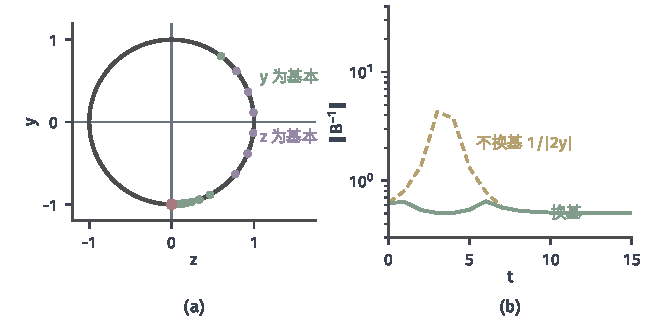
\includegraphics[width=112mm]{figures/05-optimization/06-constrained-optimization/matplotlib/feas-grg-basis/figure.pdf}
  \caption{换基的效果，问题~\eqref{eq:feas-circle}，从$(0.8,0.6)$出发，步长$1/4$。(a)迭代点的颜色表示当轮的基本变量：绿色为$y$，紫色为$z$，红点是最优解。(b)沿同一路径的$\lVert\bm{B}^{-1}\rVert$：黄色虚线是始终以$y$为基本变量时的$1/\lvert2y\rvert$，路径经过$y\approx0$附近时急剧增大；绿线是每轮换基后的值，保持有界。}
  \label{fig:feas-grg-basis}
\end{BookInlineFigure}

\paragraph{运行中要监测什么}
GRG实现要持续监测三类量：$\bm{B}$的条件数，太大就换基；原始可行性$\lVert\bm{c}(\bm{x})\rVert_\infty$和界的违反量；KKT残差，也就是式~\eqref{eq:feas-grg-signs}的违反程度。

\paragraph{每步可行不等于全局最优}
局部表示、可行恢复和换基都有条件，任何一个失败，算法就要改变动作。即使全部成功，得到的也只是满足一阶条件的点。在圆周例中，点$(y,z)=(1,0)$的约化梯度为零，它满足KKT条件，却是目标的最大点。从恰好这一点出发，方法不会移动。约束非凸时，每步可行和目标下降都推不出全局最优。

\section{方法比较}
\label{sec:feas-compare}

前面四种方法该怎样选？本节先按集合结构筛选，再谈成本。比较的前提是同一个问题确实满足所比较方法的条件，并且用相同的可行精度和相同的最优性度量。

\paragraph{先看集合}
选择的第一步是问集合支持什么运算。闭凸集合上可以选投影、线性最小化或Bregman子问题；光滑非线性等式约束只有GRG的局部消元和解方程这条路，前三种方法的保证不适用。反过来，单纯形这样的简单集合也用不着GRG。把适用集合不同的方法排成统一的优劣次序没有意义。

\paragraph{同一问题上的比较}
三种闭凸方法都能解预算例。图~\ref{fig:feas-compare}(a)显示投影梯度最快，因为投影的代价在单纯形上很低，解又落在一条边上，活动集识别后就是一维问题。

图~\ref{fig:feas-compare}(b)换成高维单纯形上的最小二乘问题，看解的稀疏性。条件梯度的非零元个数从一开始缓慢增长，始终很少；投影梯度从稠密起点迅速截断；镜像下降一直保持全部为正。条件梯度的稀疏只是说输出的表示短，并不说明它更准确。

\begin{BookInlineFigure}
  \centering
  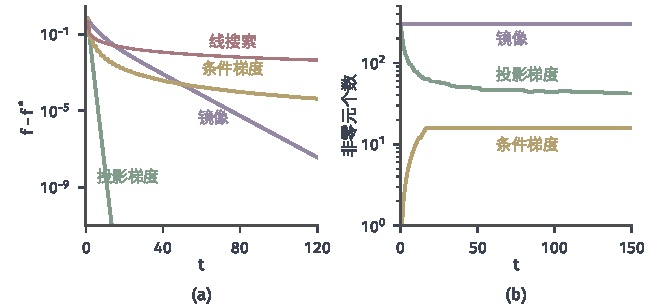
\includegraphics[width=112mm]{figures/05-optimization/06-constrained-optimization/matplotlib/feas-compare/figure.pdf}
  \caption{同一单纯形问题上的比较。(a)预算例的迄今最小目标差：绿线投影梯度，紫线镜像下降，黄线条件梯度（预定序列），红线条件梯度（线搜索）。(b)$n=300$的单纯形最小二乘，随机矩阵$\bm{A}\in\mathbb{R}^{60\times300}$（种子固定），绿线投影梯度和紫线镜像下降从均匀分布出发，黄线条件梯度从一个顶点出发，纵轴是非零元个数。}
  \label{fig:feas-compare}
\end{BookInlineFigure}

表~\ref{tab:feas-compare}归纳了单纯形上每轮的成本和结构。总成本是每轮成本乘以达到相同精度所需的轮数，只看其中一个因子会得出错误的结论。

\begin{BookInlineTable}
  \centering
  \caption{$n$维单纯形上三种方法每轮的额外运算（梯度计算另计）。}
  \label{tab:feas-compare}
  \begin{tabular}{llll}
   \toprule
   方法 & 额外运算 & 输出结构 & 活动约束\\
   \midrule
   投影梯度 & 排序，$O(n\log n)$ & 可稀疏 & 有限步后常被识别\\
   条件梯度 & 找最小分量，$O(n)$ & 顶点的短组合 & 基本流程难以识别\\
   镜像下降 & 乘法与归一化，$O(n)$ & 全部为正 & 不精确识别\\
   \bottomrule
  \end{tabular}
\end{BookInlineTable}

\subsection{内层精度}
\label{sec:feas-compare-inner}

每种方法的子问题都可能只能近似求解。这些内层误差分别影响哪里，又该解到多准？

\paragraph{误差进入的位置}
表~\ref{tab:feas-inner}按方法列出内层误差的去向。投影和GRG的恢复直接影响可行性，线性最小化的误差只影响下降和证书，因为不精确的顶点仍在集合内。

\begin{BookInlineTable}
  \centering
  \caption{内层误差的影响。}
  \label{tab:feas-inner}
  \begin{tabular}{llll}
   \toprule
   内层计算 & 可行性 & 下降 & 停止检验\\
   \midrule
   投影 & 可能略不可行 & 式~\eqref{eq:feas-inexact-recursion} & 残差误差$\varepsilon/\alpha$\\
   线性最小化 & 不受影响 & 式~\eqref{eq:feas-inexact-lmo} & 间隙加$\varepsilon$\\
   镜像子问题 & 视解法而定 & 三点关系多余项 & 同步记录误差\\
   GRG恢复 & 残差至多$\varepsilon_c$ & $F$的值有误差 & 须检查$\bm{c}$\\
   \bottomrule
  \end{tabular}
\end{BookInlineTable}

熵势在单纯形上的子问题有闭式解，归一化的舍入误差可以忽略。一般的集合上，镜像子问题也要迭代求解，并且三点关系~\eqref{eq:feas-three-point}多出误差项，处理方式和近似投影类似。

\paragraph{按外层精度安排内层}
外层离解还远时，把内层解到很高的精度是浪费；外层接近收敛时，内层误差又会成为瓶颈。前面的递推说明了这一点：式~\eqref{eq:feas-inexact-lmo}让线性最小化的容差随$\alpha^{(t)}$减小，式~\eqref{eq:feas-inexact-recursion}说明投影容差决定了误差的平台。常用做法是把内层容差设成外层当前残差的一个比例。

GRG的恢复容差则有一个硬性的下限要求：它决定了输出点的可行程度，至少要达到最终要求的约束精度。

\paragraph{成本要算全}
GRG每轮的成本不只是外层更新，要把下面各项都算进去：
\begin{itemize}
 \item 线搜索中重复的恢复，每次试探步长都要解一次非线性方程；
 \item 每次恢复中的Newton迭代，各需一次约束计算和一次线性方程求解；
 \item Jacobian矩阵的更新与$\bm{B}$的分解，稠密时分解约需$p^3$量级的运算；
 \item 换基之后的重新分解或分解修正。
\end{itemize}

上面圆周例的第三轮就要试探五个步长，其中四个失败或被拒绝，这些计算都要计入总成本。投影梯度的回溯同样要计入重复投影的次数。比较方法时，统计的是这些基本运算的总次数，而不是外层轮数。

\subsection{结果检验}
\label{sec:feas-compare-check}

算法停下来之后，应该报告什么数字来证明结果可用？

\paragraph{凸问题}
凸问题可以报告目标差的上界。条件梯度的间隙$\Gamma$直接就是这样的上界。单纯形上计算$\Gamma$只要$O(n)$，投影梯度或镜像下降也可以顺便算一个间隙作为证书。

没有线性最小化可用时，投影残差也能给出上界。在定理~\ref{thm:feas-pgd-convex}的证明中取$\mu=0$，$\alpha=1/L$，$\bm{y}=\bm{x}^\star$，由内积的上界和残差的定义，得到
\begin{equation}
 f(\bm{x}^{+})-f^\star\leq\lVert\bm{G}_\alpha(\bm{x})\rVert_2\lVert\bm{x}^{+}-\bm{x}^\star\rVert_2+\frac{1}{2L}\lVert\bm{G}_\alpha(\bm{x})\rVert_2^2.
 \label{eq:feas-residual-gap}
\end{equation}
这需要知道到解的距离的上界，比如集合的直径，否则残差小不能换算成目标差小。

\paragraph{非凸光滑问题}
目标非凸时报告驻定度量，$\lVert\bm{G}_\alpha\rVert_2$或$\Gamma$都可以，同时要说明步长，并明确它只检验一阶条件。

\paragraph{GRG}
GRG的报告必须回到原问题的形式：$\lVert\bm{c}(\bm{x})\rVert_\infty$、界的违反量、以及完整的KKT残差。只看约化梯度的范数是不够的。在圆周例的不可行点$(y,z)=(2,0)$上，公式~\eqref{eq:feas-reduced-gradient}算出$\nabla F=0$，而约束残差是$3$。约化梯度的含义依赖于“当前点在约束面上”这个前提。

\paragraph{随机方向}
大规模时梯度常常用随机估计代替。第~\ref{chap:stochastic-gradient-methods}章的分析依赖更新对噪声是线性的，这样条件期望可以直接进入更新。投影和指数映射都是非线性的，期望不能穿过去。

取$\bm{C}=[0,1]$，$x=0$，随机梯度等概率取$\pm1$，期望是零。精确梯度的投影更新留在原地，而随机更新的期望是
\[
 \mathbb{E}\bigl[P_{\bm{C}}(x-\alpha\tilde g)\bigr]=\tfrac12\alpha+\tfrac12\cdot0=\tfrac\alpha2\neq0.
\]

指数映射也是如此：
\[
 \mathbb{E}\bigl[\exp(-\alpha\tilde g)\bigr]=\cosh\alpha>1=\exp\bigl(-\alpha\,\mathbb{E}[\tilde g]\bigr).
\]

所以把随机方向接入投影或镜像更新时，要在变分不等式或三点关系那一层使用条件期望，也就是对内积取期望，然后单独控制噪声带来的二次项，不能把噪声当成在映射之外平均掉。

\section{本章小结}
\label{sec:feas-summary}

本章的问题是怎样让每个迭代点满足原约束，以及保持或恢复可行性要花多少计算。预算例给出了同一问题上的对比，圆周例说明了凸集之外的情形。

投影梯度把梯度步拉回最近点，残差$\bm{G}_\alpha$为零等价于变分不等式，$L$光滑时目标差有$1/T$的界，强凸时距离线性收缩。条件梯度只用线性最小化，靠凸组合保持可行，产生顶点的短组合，间隙$\Gamma$在凸问题上上界目标差。镜像下降把欧氏距离换成Bregman距离，在单纯形上给出保持正性的指数更新；一般次梯度分析针对平均点，只有相对光滑时目标才逐步下降。

GRG面向光滑非线性约束，通过可逆的基矩阵局部消元，按约化梯度移动非基本变量，再解方程恢复基本变量，碰界或病态时换基。它依赖的是局部可解性，与前三种方法的闭凸集假设不同，两边的保证不能互相借用。

各种方法都要分别检查原约束误差和合适的最优性残差。内层投影、线性最小化或恢复不精确时，误差要进入递推和停止检验。可行迭代还需要一个可行的起点，这个起点本身有时也要专门构造。


\chapter{惩罚与乘子方法}
\label{chap:penalty-multiplier-methods}

两家工厂要合计生产$4$个单位，产量分别为$x_1$和$x_2$，成本分别是$\tfrac12x_1^2$和$\tfrac32x_2^2$。问题写出来是
\begin{equation}
 \min_{\bm{x}\in\mathbb{R}^2}\ f(\bm{x})=\frac12x_1^2+\frac32x_2^2
 \qquad\text{s.t.}\qquad h(\bm{x})=x_1+x_2-4=0 .
 \label{eq:pm-running}
\end{equation}
消去一个变量，或者解KKT方程，可以得到$\bm{x}^\star=(3,1)$，最优值$f^\star=6$。这条约束是线性的，第~\ref{chap:feasible-iterations}章的做法可以每一步都留在直线上。一旦约束弯曲，或者有成千上万条，每一步都保持可行就可能比原问题还难。

本章走另一条路：允许迭代点暂时违反约束，让违反本身产生一个信号，再由信号把点拉回来。工厂的例子里有两种自然的信号。一种是罚款：总产量偏离$4$就按偏离量收钱。另一种是价格：总部报出一个单价，两家工厂各自决定产量，总量不够就提价，过多就降价。

这两种信号各有毛病。罚款要想把违规压到零，必须重到无穷大，内层问题随之越来越难解；价格不增加任何曲率，步子一大就来回振荡，而且目标线性时根本定不出产量。全章的路线是：先把两种信号各自讲透，第~\ref{sec:pm-quadratic}节和第~\ref{sec:pm-exact}节讲罚款，第~\ref{sec:pm-dual-ascent}节讲价格；再把它们合在一个函数里，第~\ref{sec:pm-alm}节看到两者的毛病恰好互相弥补；第~\ref{sec:pm-admm}节进一步问，变量分成两块时能否一块一块地更新。

式~\eqref{eq:pm-running}贯穿全章，用来比较各种方法。另一个例子更小，只有一个变量和一条不等式约束：
\begin{equation}
 \min_{x\in\mathbb{R}}\ x\qquad\text{s.t.}\qquad 1-x\leq0 ,
 \label{eq:pm-one-dim}
\end{equation}
它的解是$x^\star=1$，乘子$\lambda^\star=1$。下文分别称为二元例和一维例。全章讨论的一般问题是
\begin{equation}
 \min_{\bm{x}\in\mathbb{R}^n}\ f(\bm{x})
 \quad\text{s.t.}\quad g_i(\bm{x})\leq0\ (i=1,\ldots,m),\quad h_j(\bm{x})=0\ (j=1,\ldots,p),
 \label{eq:pm-problem}
\end{equation}
可行集记作$\bm{C}$。原始可行、Lagrange驻定、全局证书是三件不同的事，第~\ref{chap:constrained-optimality}章和第~\ref{chap:duality}章已经分别建立，本章每种方法结束时都要回到这三项上逐一核对。

\section{二次惩罚法}
\label{sec:pm-quadratic}

把约束换成目标里的一笔费用之后，得到的解离原问题有多远，又要付出什么代价？

\paragraph{给违规计价}
可以把约束想成预算。硬约束相当于一分钱都不许超；惩罚的做法是允许超，但超得越多罚得越狠。费用要满足两点：可行时为零，不改变可行点上的目标；违规时为正，并且最好是光滑的，这样前面的无约束方法可以直接使用。

平方正好满足这两点。等式残差$h_j$偏离零时收$h_j^2$。不等式只有$g_i>0$时才算违规，所以先取正部
\[
 [a]_+=\max\{a,0\},
\]
再平方。把两类费用加到目标上，就得到下面的函数。

\begin{definition}[二次罚函数]
\label{def:pm-quadratic-penalty}
对问题~\eqref{eq:pm-problem}和\term{罚参数}（penalty parameter）$\rho>0$，\term{二次罚函数}（quadratic penalty function）是
\begin{equation}
 Q_\rho(\bm{x})=f(\bm{x})+\frac{\rho}{2}\Bigl(\sum_{i=1}^m[g_i(\bm{x})]_+^2+\sum_{j=1}^ph_j(\bm{x})^2\Bigr).
 \label{eq:pm-quadratic-penalty}
\end{equation}
依次近似最小化$Q_\rho$并逐步增大$\rho$的做法称为\term{二次惩罚法}（quadratic penalty method）。
\end{definition}

迭代点一般从可行集外面逼近，所以这类方法也叫外点法。正部的平方虽然含有$\max$，导数却是连续的：$\phi(a)=[a]_+^2$在$a<0$时为零，在$a>0$时为$a^2$，两边在$a=0$处的导数都是$0$，因此$\phi'(a)=2[a]_+$。由链式法则，当$f,g_i,h_j$都连续可微时，
\begin{equation}
 \nabla Q_\rho(\bm{x})=\nabla f(\bm{x})+\rho\sum_{i=1}^m[g_i(\bm{x})]_+\nabla g_i(\bm{x})+\rho\sum_{j=1}^ph_j(\bm{x})\nabla h_j(\bm{x}).
 \label{eq:pm-quadratic-gradient}
\end{equation}
要注意$\phi''$在$a=0$处跳跃，所以有不等式约束时$Q_\rho$一般只是一阶连续可微，二阶导数在约束边界上不连续。

\begin{example}[一维例的二次罚]
\label{ex:pm-quadratic-one-dim}
式~\eqref{eq:pm-one-dim}的$g(x)=1-x$，罚函数是
\[
 Q_\rho(x)=x+\frac{\rho}{2}[1-x]_+^2 .
\]
当$x\geq1$时，$Q_\rho'(x)=1>0$，这部分没有驻点。当$x<1$时，
\[
 Q_\rho'(x)=1-\rho(1-x).
\]
令其为零，解出
\[
 x_\rho=1-\frac1\rho .
\]
$Q_\rho$是凸函数，所以这个驻点是全局最小点。它落在可行集外，违规量恰好是$1/\rho$。
\end{example}

图~\ref{fig:pm-quad-1d}画出$\rho=1,2,5$时的$Q_\rho$。绿点随$\rho$增大向右移动，始终停在竖线左边，不可行。绿点的高度是$Q_\rho(x_\rho)=1-1/(2\rho)$，比原问题的最优值$1$低。可见罚目标的值既不是原目标，也不是最优值的上界，降低罚目标和满足原约束是两件要分别检查的事。

\begin{BookInlineFigure}
  \centering
  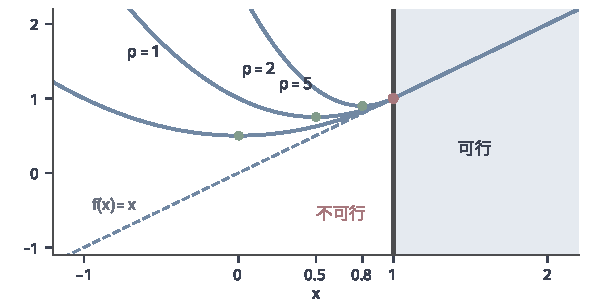
\includegraphics[width=100mm]{figures/05-optimization/06-constrained-optimization/matplotlib/pm-quad-1d/figure.pdf}
  \caption{一维例的二次罚函数，$\rho=1,2,5$。蓝色实线是$Q_\rho$，蓝色虚线是原目标$f(x)=x$，浅蓝区域是可行集，深灰竖线是约束边界。绿点是$Q_\rho$的最小点$x_\rho=1-1/\rho$，红点是原问题的解。有限的$\rho$下最小点总在边界左侧。}
  \label{fig:pm-quad-1d}
\end{BookInlineFigure}

\paragraph{力的平衡}
为什么有限的$\rho$总留下违规？把驻点方程$\rho(1-x_\rho)=1$读成力的平衡。目标以大小为$1$的力把$x$往左拉，罚项像一根劲度为$\rho$的弹簧往右推。弹簧必须被拉长才有力，要平衡$1$的力就得拉长$1/\rho$。弹簧越硬，拉长越少，但只要力不为零，拉长量就不为零。

这个力的大小$\rho(1-x_\rho)=1$恰好是最优乘子$\lambda^\star=1$。第~\ref{chap:constrained-optimality}章说过，乘子度量约束对目标的反作用力。这里违规量乘罚参数等于乘子，并不是一维例的巧合，后面会看到它的一般形式。类比也有失效的地方：真实的弹簧两边都有力，而不等式的罚项只在违规一侧起作用。

\begin{example}[二元例的二次罚]
\label{ex:pm-quadratic-running}
对式~\eqref{eq:pm-running}，罚函数是
\[
 Q_\rho(\bm{x})=\frac12x_1^2+\frac32x_2^2+\frac\rho2(x_1+x_2-4)^2 .
\]
令梯度为零，得到两个线性方程：
\[
 (1+\rho)x_1+\rho x_2=4\rho,\qquad \rho x_1+(3+\rho)x_2=4\rho .
\]
两式相减得$x_1=3x_2$。代回第二式，解出
\begin{equation}
 x_2(\rho)=\frac{4\rho}{3+4\rho},\qquad x_1(\rho)=\frac{12\rho}{3+4\rho}.
 \label{eq:pm-running-penalty-solution}
\end{equation}
由此算出约束残差
\begin{equation}
 h(\bm{x}(\rho))=-\frac{12}{3+4\rho}.
 \label{eq:pm-running-penalty-residual}
\end{equation}
它在$\rho\to\infty$时以$1/\rho$的速度趋于零，而$\rho h(\bm{x}(\rho))$趋于$-3$，正是$\nu^\star$。
\end{example}

图~\ref{fig:pm-penalty-contours}是同一个例子的二维图景。深灰直线是约束，绿点是$Q_\rho$的最小点。$\rho$增大时等高线沿直线方向被拉长，绿点向红点靠近。

\begin{BookInlineFigure}
  \centering
  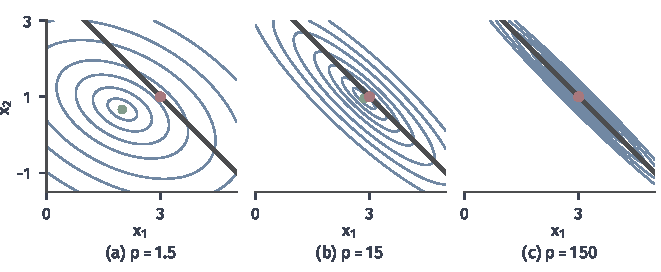
\includegraphics[width=112mm]{figures/05-optimization/06-constrained-optimization/matplotlib/pm-penalty-contours/figure.pdf}
  \caption{二元例中$Q_\rho$的等高线（蓝）。深灰直线是约束$x_1+x_2=4$，绿点是$Q_\rho$的最小点，红点是原问题的解$(3,1)$。$\rho$增大时最小点靠近解，等高线同时变成贴着约束的狭长椭圆。}
  \label{fig:pm-penalty-contours}
\end{BookInlineFigure}

\subsection{罚参数的更新}
\label{sec:pm-rho-update}

\paragraph{主要思想}
式~\eqref{eq:pm-running-penalty-residual}提示一开始就把$\rho$取得很大，一次解完。这样做的问题在于，$\rho$大的罚问题很难解，本节后面会算出来。如果从不好的初值开始，内层算法可能花大量步数才能进入解的附近。

合理的做法是沿着$\rho$的路径走。先取较小的$\rho$，解一个容易的问题；再放大$\rho$，以上一轮的解作为初值。$\rho$只放大有限倍时，新解离旧解不远，这叫\term{热启动}（warm start）。外层循环的结构如图~\ref{fig:pm-outer-loop}所示。

\begin{BookInlineFigure}
  \centering
  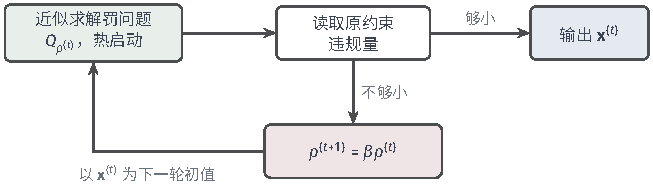
\includegraphics[width=110mm]{figures/05-optimization/06-constrained-optimization/tikz/pm-outer-loop/figure.pdf}
  \caption{二次惩罚法的外层循环。绿框是内层的无约束求解，蓝框是输出；判断依据是原约束的违规量，而不是罚目标的大小。只有违规量不够小时才放大罚参数（红框）。}
  \label{fig:pm-outer-loop}
\end{BookInlineFigure}

这里有两个容差，分工不同。内层容差$\omega^{(t)}$控制$\lVert\nabla Q_{\rho^{(t)}}(\bm{x}^{(t)})\rVert_2$，说明这一轮的罚问题解得多准。外层容差$\varepsilon$控制原约束的违规量，说明原问题的可行性够不够。内层梯度很小，只说明罚问题解好了，不能据此宣布原问题已解。

放大规则取固定倍数$\beta>1$，并记录乘子估计：
\begin{equation}
 \rho^{(t+1)}=\beta\rho^{(t)},\qquad
 \nu_j^{(t)}=\rho^{(t)}h_j(\bm{x}^{(t)}),\qquad
 \lambda_i^{(t)}=\rho^{(t)}[g_i(\bm{x}^{(t)})]_+ .
 \label{eq:pm-penalty-update}
\end{equation}
这组估计的来历可以从式~\eqref{eq:pm-quadratic-gradient}读出：把它们代入，$\nabla Q_{\rho}$恰好是Lagrange函数对$\bm{x}$的梯度。内层求解到梯度为零，就等于Lagrange驻定条件在这组估计下成立。

\paragraph{计算过程}
以二元例为例，内层用步长为$1/L$的梯度法，其中$L$是$\nabla^2Q_\rho$的最大特征值。

\needspace{6\baselineskip}
\paragraph{变量}
\begin{itemize}
 \item $\bm{x}^{(t)}\in\mathbb{R}^n$：第$t$轮罚问题的近似解。例中$n=2$。
 \item $\rho^{(t)}>0$：罚参数，放大倍数为$\beta>1$。
 \item $\varepsilon$、$\omega^{(t)}$：外层违规容差、内层梯度容差。
\end{itemize}

\paragraph{初始化}
取初值$\bm{x}^{(-1)}$、$\rho^{(0)}>0$和$\beta$。例中$\bm{x}^{(-1)}=(0,0)$，$\rho^{(0)}=1.5$，$\beta=10$，外层容差$\varepsilon=0.05$，内层容差取常数$\omega^{(t)}=10^{-3}$。

\needspace{6\baselineskip}
\paragraph{每轮更新}
\begin{enumerate}
 \item 从$\bm{x}^{(t-1)}$出发近似最小化$Q_{\rho^{(t)}}$，直到梯度范数不超过$\omega^{(t)}$。例中第一轮用了$21$个梯度步，结果接近式~\eqref{eq:pm-running-penalty-solution}的精确解，以下数值用精确解给出：
 \[
  \bm{x}^{(0)}=\Bigl(2,\ \frac23\Bigr).
 \]

 \item 计算违规量。例中第一轮
 \[
  h(\bm{x}^{(0)})=-\frac43,\qquad \lvert h(\bm{x}^{(0)})\rvert>\varepsilon .
 \]
 \item 若违规量不超过$\varepsilon$，结束；否则由式~\eqref{eq:pm-penalty-update}放大罚参数并记录乘子估计。例中第一轮
 \[
  \rho^{(1)}=15,\qquad \nu^{(0)}=1.5\times\Bigl(-\frac43\Bigr)=-2 .
 \]
\end{enumerate}
例中第二轮从$\bm{x}^{(0)}$热启动，用了$107$个梯度步，得到
\[
 \bm{x}^{(1)}=\Bigl(\frac{20}{7},\ \frac{20}{21}\Bigr),\qquad
 h(\bm{x}^{(1)})=-\frac{4}{21}\approx-0.190 .
\]
乘子估计是$\nu^{(1)}=-\tfrac{20}{7}\approx-2.857$。
违规量仍大于$0.05$，于是$\rho^{(2)}=150$。第三轮用了$725$个梯度步，得到
\[
 \bm{x}^{(2)}=\Bigl(\frac{200}{67},\ \frac{200}{201}\Bigr),\qquad
 h(\bm{x}^{(2)})=-\frac{4}{201}\approx-0.020 .
\]
乘子估计是$\nu^{(2)}=-\tfrac{200}{67}\approx-2.985$。

结束条件是违规量不超过$\varepsilon$，例中在第三轮满足。最终得到$\bm{x}^{(2)}\approx(2.985,0.995)$，目标值$f(\bm{x}^{(2)})\approx5.940$，略低于$f^\star=6$，这是因为点还不可行。三轮的梯度步数依次是$21$、$107$、$725$，几乎全部花在最后一轮上。步数为什么增长这么快，正是下一小节要回答的。

\subsection{极限与病态}
\label{sec:pm-limit}

这一小节回答两个问题：$\rho\to\infty$时迭代点到底趋于什么，以及这条路有多贵。

\paragraph{全局解的极限}
先看最理想的情形，每一轮都得到罚问题的全局最小点。此时可以把罚目标与任意一个可行点比较，这个比较给出全部结论。

\begin{theorem}[二次惩罚法的全局极限]
\label{thm:pm-quadratic-limit}
设$f$、$g_i$、$h_j$在$\mathbb{R}^n$上连续，可行集$\bm{C}$非空，且$f$在$\mathbb{R}^n$上有下界$f_{\mathrm{low}}$。设$\rho^{(t)}\to\infty$，每个$\bm{x}^{(t)}$都是$Q_{\rho^{(t)}}$的全局最小点。记
\begin{equation}
 v(\bm{x})=\sum_{i=1}^m[g_i(\bm{x})]_+^2+\sum_{j=1}^ph_j(\bm{x})^2 .
 \label{eq:pm-violation-square}
\end{equation}
则对任一可行点$\bar{\bm{x}}\in\bm{C}$，有
\begin{equation}
 v(\bm{x}^{(t)})\leq\frac{2\bigl(f(\bar{\bm{x}})-f_{\mathrm{low}}\bigr)}{\rho^{(t)}},
 \label{eq:pm-quadratic-violation-bound}
\end{equation}
并且$\{\bm{x}^{(t)}\}$的每个聚点都是原问题的全局最优解。
\end{theorem}

\begin{proof}
可行点上罚项为零，$Q_{\rho^{(t)}}(\bar{\bm{x}})=f(\bar{\bm{x}})$。$\bm{x}^{(t)}$是全局最小点，所以
\[
 f(\bm{x}^{(t)})+\frac{\rho^{(t)}}{2}v(\bm{x}^{(t)})\leq f(\bar{\bm{x}}).
\]
左边第一项用$f_{\mathrm{low}}$放缩，整理即得式~\eqref{eq:pm-quadratic-violation-bound}。

设$\hat{\bm{x}}$是一个聚点，子列收敛到它。$v$连续，而式~\eqref{eq:pm-quadratic-violation-bound}的右边趋于零，所以$v(\hat{\bm{x}})=0$，即$\hat{\bm{x}}$可行。

上面的不等式中罚项非负，去掉后得到
\[
 f(\bm{x}^{(t)})\leq f(\bar{\bm{x}}).
\]
沿子列取极限，由$f$连续得$f(\hat{\bm{x}})\leq f(\bar{\bm{x}})$。$\bar{\bm{x}}$是任取的可行点，所以$\hat{\bm{x}}$全局最优。
\end{proof}

各条件的作用分得很清楚。可行集非空提供了比较点$\bar{\bm{x}}$。下界把违规量和$\rho$联系起来。连续性保证极限可行，并让目标比较传到极限。“全局最小点”是证明的关键一步，局部解不能和远处的可行点比较。定理也不保证聚点存在：序列可能跑向无穷远，要排除这种情形，还需要类似水平集有界的条件。

去掉下界会怎样？考虑$\min x^3$，$x\geq0$，解是$x^\star=0$。罚函数在$x<0$时等于$x^3+\tfrac\rho2x^2$，$x\to-\infty$时趋于$-\infty$，所以对任何$\rho$都没有全局最小点。图~\ref{fig:pm-failures}(a)画出了这种情形：$x=0$附近有一个局部的谷，越过左侧的小山就一路下降。原问题完全正常，罚问题却无下界。

\paragraph{近似解的极限}
实际算法只能给出梯度小的点，通常连局部最小都不能保证。这时比较可行点的论证失效，能说的话变少，并且要多加条件。下面只写等式约束，记$\bm{h}(\bm{x})=(h_1(\bm{x}),\ldots,h_p(\bm{x}))$，$\bm{J}(\bm{x})\in\mathbb{R}^{p\times n}$是它的Jacobian矩阵。

\begin{theorem}[近似驻点的极限]
\label{thm:pm-quadratic-approximate}
设$f,h_j$连续可微，$\rho^{(t)}\to\infty$，并且
\begin{equation}
 \lVert\nabla Q_{\rho^{(t)}}(\bm{x}^{(t)})\rVert_2\leq\omega^{(t)}\to0 .
 \label{eq:pm-inner-accuracy}
\end{equation}
设$\hat{\bm{x}}$是$\{\bm{x}^{(t)}\}$的聚点，则$\hat{\bm{x}}$是$\tfrac12\lVert\bm{h}\rVert_2^2$的驻点。若进一步$\hat{\bm{x}}$可行且$\bm{J}(\hat{\bm{x}})$行满秩，则沿收敛到$\hat{\bm{x}}$的子列有
\begin{equation}
 \rho^{(t)}\bm{h}(\bm{x}^{(t)})\to\hat{\bm{\nu}},\qquad
 \nabla f(\hat{\bm{x}})+\bm{J}(\hat{\bm{x}})^\top\hat{\bm{\nu}}=\bm{0},
 \label{eq:pm-multiplier-limit}
\end{equation}
即$(\hat{\bm{x}},\hat{\bm{\nu}})$满足KKT条件。
\end{theorem}

\begin{proof}
记$\bm{e}^{(t)}=\nabla Q_{\rho^{(t)}}(\bm{x}^{(t)})$，$\bm{e}^{(t)}\to\bm{0}$。为简化写法，下面的量都沿子列取，并省略$\bm{x}^{(t)}$的自变量。由梯度公式，
\[
 \nabla f+\rho^{(t)}\bm{J}^\top\bm{h}=\bm{e}^{(t)}.
\]
两边除以$\rho^{(t)}$，得到
\[
 \bm{J}^\top\bm{h}=\frac{\bm{e}^{(t)}-\nabla f}{\rho^{(t)}}.
\]
右边的分子有界，分母趋于无穷，取极限得
\[
 \bm{J}(\hat{\bm{x}})^\top\bm{h}(\hat{\bm{x}})=\bm{0}.
\]
左边正是$\tfrac12\lVert\bm{h}\rVert_2^2$的梯度，第一个结论成立。

再设$\hat{\bm{x}}$可行且$\bm{J}(\hat{\bm{x}})$行满秩。$\bm{J}\bm{J}^\top$连续且极限可逆，所以$t$足够大时可逆。用$\bm{J}$左乘第一个等式再求逆，解出
\[
 \rho^{(t)}\bm{h}=(\bm{J}\bm{J}^\top)^{-1}\bm{J}\bigl(\bm{e}^{(t)}-\nabla f\bigr).
\]
右边收敛，记极限为$\hat{\bm{\nu}}$。把$\rho^{(t)}\bm{h}\to\hat{\bm{\nu}}$代回第一个等式取极限，即得式~\eqref{eq:pm-multiplier-limit}。
\end{proof}

这个定理有两点值得注意。第一，$\hat{\bm{x}}$完全可能不可行，它只是约束残差平方的驻点。第二，定理的结论停在KKT点，和全局最优还差得远。

下面的例子显示第一点确实会发生。取
\[
 \min_x\ \frac12x^2\qquad\text{s.t.}\qquad h(x)=x^3-3x+3=0 .
\]
三次方程只有一个实根$x^\star\approx-2.104$，这也是唯一的可行点。$h$在$x=1$处有局部极小值$h(1)=1$，所以$\tfrac12h^2$在这里有一个不可行的局部谷。图~\ref{fig:pm-failures}(b)中绿点是$Q_3$在这个谷里的局部最小点。

取$\rho=10$和$\rho=100$，用二分法解$Q_\rho'(x)=0$，得到谷中的驻点分别是
\[
 x_{10}\approx0.9835,\qquad x_{100}\approx0.9983 .
\]
这两个点上$Q_\rho$的梯度为零，$h$却约等于$1$。放大$\rho$只会让点更靠近$x=1$，乘子估计$\rho h$随之发散。乘子估计发散正是不可行极限的常见信号。

\begin{BookInlineFigure}
  \centering
  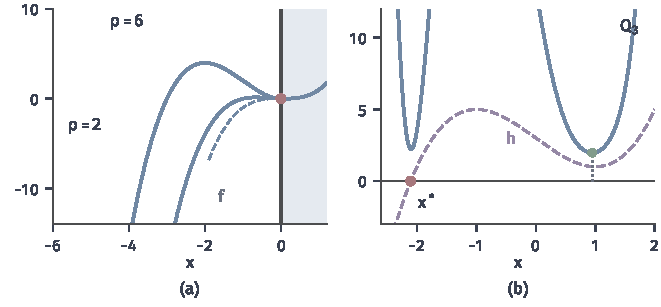
\includegraphics[width=112mm]{figures/05-optimization/06-constrained-optimization/matplotlib/pm-failures/figure.pdf}
  \caption{二次惩罚法的两种失败。(a)$\min x^3$，$x\geq0$：蓝色实线是$\rho=2,6$的罚函数，虚线是$f$的一段，浅蓝区域可行，红点是解；$x\to-\infty$时罚函数无下界。(b)$\min\tfrac12x^2$，$h(x)=x^3-3x+3=0$：紫色虚线是$h$，蓝线是$Q_3$，红点是唯一的可行点，绿点是不可行的局部最小点。}
  \label{fig:pm-failures}
\end{BookInlineFigure}

\paragraph{法向曲率的增长}
剩下的问题是代价。对等式约束的罚函数求二阶导，得到
\begin{equation}
 \nabla^2Q_\rho=\nabla^2f+\rho\sum_{j=1}^ph_j\nabla^2h_j+\rho\bm{J}^\top\bm{J}.
 \label{eq:pm-penalty-hessian}
\end{equation}
由定理~\ref{thm:pm-quadratic-approximate}，$\rho h_j$在解附近接近有限的乘子，前两项之和接近Lagrange函数的Hessian，大小不随$\rho$增长。第三项却正比于$\rho$，它只在$\bm{J}$的行空间里起作用，也就是约束的法方向上。

线性约束的二次目标可以把这件事算清楚。设目标和约束分别是
\[
 f(\bm{x})=\frac12\bm{x}^\top\bm{G}\bm{x}-\bm{d}^\top\bm{x},\qquad\bm{h}(\bm{x})=\bm{A}\bm{x}-\bm{b},
\]
其中$\bm{A}\in\mathbb{R}^{p\times n}$，$p<n$，$\bm{G}$半正定。此时$\nabla^2Q_\rho=\bm{G}+\rho\bm{A}^\top\bm{A}$不依赖$\bm{x}$。

\begin{lemma}[罚函数Hessian的条件数]
\label{lem:pm-penalty-condition}
设$\bm{A}\neq\bm{0}$，$\bm{Z}$的列是$\operatorname{null}(\bm{A})$的一组标准正交基，矩阵$\bm{Z}^\top\bm{G}\bm{Z}$正定，$\sigma_{\max}(\bm{A})$是$\bm{A}$的最大奇异值。记$\bm{H}_\rho=\bm{G}+\rho\bm{A}^\top\bm{A}$。当$\bm{H}_\rho$正定时，有
\begin{equation}
 \lambda_{\max}(\bm{H}_\rho)\geq\rho\,\sigma_{\max}(\bm{A})^2,\qquad
 \lambda_{\min}(\bm{H}_\rho)\leq\lambda_{\min}(\bm{Z}^\top\bm{G}\bm{Z}),
 \label{eq:pm-penalty-eigen-bounds}
\end{equation}
于是条件数满足
\begin{equation}
 \kappa(\bm{H}_\rho)\geq\frac{\rho\,\sigma_{\max}(\bm{A})^2}{\lambda_{\min}(\bm{Z}^\top\bm{G}\bm{Z})}.
 \label{eq:pm-penalty-condition}
\end{equation}
\end{lemma}

\begin{proof}
两个界都来自Rayleigh商。设$\bm{u}$是$\bm{A}$对应最大奇异值的单位右奇异向量。由$\bm{G}$半正定，
\[
 \lambda_{\max}(\bm{H}_\rho)\geq\bm{u}^\top\bm{H}_\rho\bm{u}\geq\rho\lVert\bm{A}\bm{u}\rVert_2^2=\rho\,\sigma_{\max}(\bm{A})^2 .
\]
再取单位向量$\bm{w}$，使它达到$\bm{Z}^\top\bm{G}\bm{Z}$的最小特征值，并令$\bm{y}=\bm{Z}\bm{w}$。$\bm{y}$是单位向量且$\bm{A}\bm{y}=\bm{0}$，所以罚项消失：
\[
 \lambda_{\min}(\bm{H}_\rho)\leq\bm{y}^\top\bm{H}_\rho\bm{y}=\bm{w}^\top\bm{Z}^\top\bm{G}\bm{Z}\bm{w}=\lambda_{\min}(\bm{Z}^\top\bm{G}\bm{Z}).
\]
两式相除，即得式~\eqref{eq:pm-penalty-condition}。
\end{proof}

几何上看，$\bm{H}_\rho$把空间分成两部分：沿约束的切方向，曲率不受$\rho$影响；沿法方向，曲率约正比于$\rho$。这就是图~\ref{fig:pm-penalty-contours}里等高线越来越狭长的原因。

二元例中$\bm{G}=\operatorname{diag}(1,3)$，$\bm{A}=(1,1)$，$\sigma_{\max}(\bm{A})^2=2$。切方向是单位向量$(1,-1)/\sqrt2$，切向曲率是
\[
 \bm{Z}^\top\bm{G}\bm{Z}=\frac{1+3}{2}=2 .
\]
下表给出$\bm{H}_\rho$的实际特征值，最小特征值逐渐接近切向曲率$2$，最大特征值约等于$2\rho$。

\begin{BookInlineTable}
  \centering
  \begin{tabular}{@{}rrrr@{}}
    \toprule
    $\rho$ & $\lambda_{\min}$ & $\lambda_{\max}$ & $\kappa$\\
    \midrule
    $1.5$ & $1.697$ & $5.303$ & $3.1$\\
    $15$ & $1.967$ & $32.03$ & $16.3$\\
    $150$ & $1.997$ & $302.0$ & $151.3$\\
    $1500$ & $2.000$ & $3002$ & $1501$\\
    \bottomrule
  \end{tabular}
  \caption{二元例中罚函数Hessian的特征值与条件数。}
  \label{tab:pm-penalty-condition}
\end{BookInlineTable}

图~\ref{fig:pm-conditioning}把精度和代价放在一起。(a)是违规量，$\rho$放大十倍，违规量缩小十倍。(b)是条件数和梯度步数，$\rho$放大十倍，条件数也放大十倍，每轮的梯度步数增长的倍数相近。

\begin{BookInlineFigure}
  \centering
  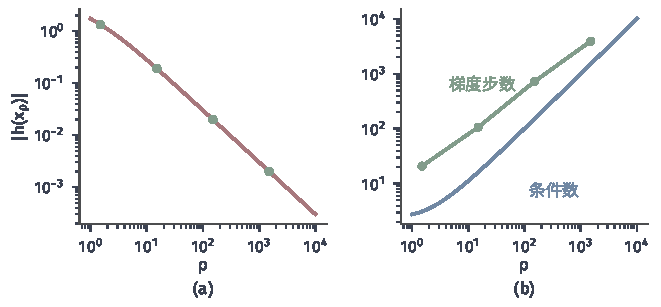
\includegraphics[width=112mm]{figures/05-optimization/06-constrained-optimization/matplotlib/pm-conditioning/figure.pdf}
  \caption{二元例中罚参数的收益与代价，双对数坐标。(a)精确罚解的违规量$12/(3+4\rho)$，绿点是$\rho=1.5,15,150,1500$。(b)蓝线是$\nabla^2Q_\rho$的条件数，绿线是热启动的梯度法（步长$1/L$，梯度容差$10^{-3}$）在各轮用的步数。}
  \label{fig:pm-conditioning}
\end{BookInlineFigure}

梯度法的困难可以直接看到。图~\ref{fig:pm-gd-penalty}从同一点出发各走$25$步。$\rho=1.5$时点很快到达最小点附近；$\rho=15$时第一步几乎只修正法向，点落到直线旁边，然后沿狭长山谷缓慢爬行，$25$步还没有走到。步长受最大曲率限制，只能取$1/L\approx1/(2\rho)$，切方向每步却只能修正很小一部分。

\begin{BookInlineFigure}
  \centering
  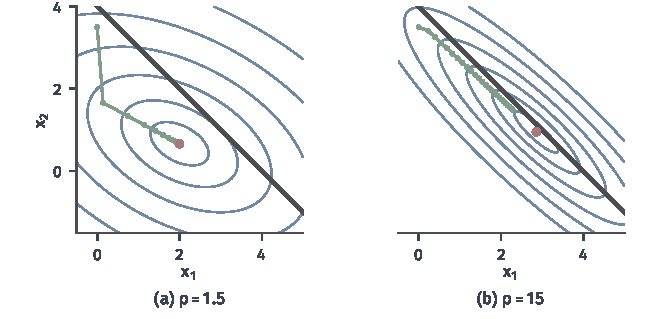
\includegraphics[width=112mm]{figures/05-optimization/06-constrained-optimization/matplotlib/pm-gd-penalty/figure.pdf}
  \caption{梯度法在$Q_\rho$上的路径，起点$(0,3.5)$，步长$1/L$，共$25$步。蓝线是$Q_\rho$的等高线，深灰直线是约束，绿色折线是迭代路径，红点是$Q_\rho$的最小点。(a)$\rho=1.5$，几步后接近最小点。(b)$\rho=15$，先快速到达山谷，再沿谷底缓慢前进。}
  \label{fig:pm-gd-penalty}
\end{BookInlineFigure}

病态是否致命，取决于内层用什么方法。Newton法不怕目标的简单伸缩，但线性方程组$\bm{H}_\rho\bm{d}=-\nabla Q_\rho$的系数矩阵本身条件数很差。引入$\bm{w}=\rho\bm{A}\bm{d}$，可以把它等价地写成
\begin{equation}
 \begin{pmatrix}\bm{G}&\bm{A}^\top\\\bm{A}&-\rho^{-1}\bm{I}\end{pmatrix}
 \begin{pmatrix}\bm{d}\\\bm{w}\end{pmatrix}
 =\begin{pmatrix}-\nabla Q_\rho\\\bm{0}\end{pmatrix}.
 \label{eq:pm-penalty-augmented-system}
\end{equation}
$\rho\to\infty$时这个系统趋于一个不含大数的KKT矩阵，数值上稳定得多。这个变换改善的是线性代数的数值误差，并不减少外层要解的问题个数。一阶方法没有这种办法。第~\ref{sec:pm-alm}节要给出另一条出路：不把$\rho$推向无穷。

\section{精确惩罚法}
\label{sec:pm-exact}

上一节的二次罚必须把$\rho$推向无穷，原因就在罚项本身：平方函数在零点的斜率是零。可行边界上，罚项完全没有回推的力，目标只要有一点斜率，点就会越过边界，直到弹簧被拉长。这就需要回答：换一种在边界上就有斜率的罚项，有限的$\rho$能否直接得到原问题的解？

\paragraph{一次罚函数}
把平方换成绝对值和正部本身，在零点就有了尖角：

\begin{definition}[一次罚函数]
\label{def:pm-exact-penalty}
对问题~\eqref{eq:pm-problem}和$\rho>0$，记总违规量
\begin{equation}
 V(\bm{x})=\sum_{i=1}^m[g_i(\bm{x})]_++\sum_{j=1}^p\lvert h_j(\bm{x})\rvert ,
 \label{eq:pm-total-violation}
\end{equation}
称
\begin{equation}
 E_\rho(\bm{x})=f(\bm{x})+\rho V(\bm{x})
 \label{eq:pm-exact-penalty}
\end{equation}
为\term{一次罚函数}（$\ell_1$ penalty function）。若存在有限的$\rho$，使$E_\rho$的最小点就是原问题的最小点，就称这个罚函数是\term{精确罚函数}（exact penalty function）。
\end{definition}

“精确”说的是两个问题的解之间的对应关系。它并不表示数值上已经把子问题解到了机器精度，也不表示算法可以一步得到解。

\begin{example}[一维例的一次罚]
\label{ex:pm-exact-one-dim}
式~\eqref{eq:pm-one-dim}的一次罚函数是
\[
 E_\rho(x)=x+\rho[1-x]_+ .
\]
$x>1$时斜率是$1$，$x<1$时斜率是$1-\rho$。结果按$\rho$分成三种情形：
\begin{itemize}
 \item $\rho<1$时，$x<1$的一侧斜率为正，$x\to-\infty$时$E_\rho\to-\infty$，没有最小点；
 \item $\rho=1$时，$x\leq1$的整条射线上$E_\rho\equiv1$，最小点集合比原问题的解大；
 \item $\rho>1$时，$E_\rho$在$x=1$处由负斜率转为正斜率，$x=1$是唯一最小点。
\end{itemize}
门槛恰好是$\lambda^\star=1$。
\end{example}

图~\ref{fig:pm-exact-1d}(a)画出这三种情形。尖角的作用从图上一眼可见：只要左边的斜率足够陡，最低点就被“钉”在尖角上，不需要$\rho$继续增大。这和一元绝对值函数的最小点停在零点，是同一种机制。

\begin{BookInlineFigure}
  \centering
  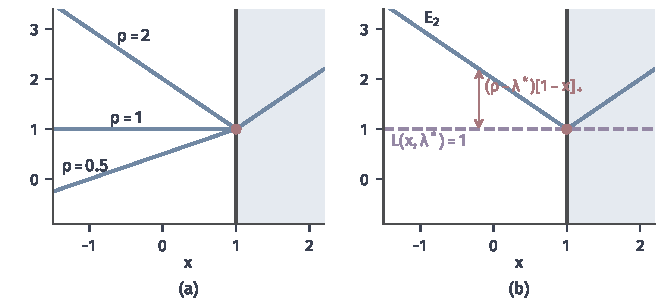
\includegraphics[width=112mm]{figures/05-optimization/06-constrained-optimization/matplotlib/pm-exact-1d/figure.pdf}
  \caption{一维例的一次罚函数。浅蓝区域可行，深灰竖线是约束边界，红点是解$x^\star=1$。(a)蓝线是$\rho=0.5,1,2$的$E_\rho$：$\rho<1$无下界，$\rho=1$左侧水平，$\rho>1$最小点就是$x^\star$。(b)蓝线是$E_2$，紫色虚线是Lagrange函数$\mathcal{L}(x,\lambda^\star)\equiv1$，$E_2$在它上方，红色箭头是两者之差。}
  \label{fig:pm-exact-1d}
\end{BookInlineFigure}

\paragraph{二元例的比较}
式~\eqref{eq:pm-running}的一次罚函数是
\[
 E_\rho(\bm{x})=\frac12x_1^2+\frac32x_2^2+\rho\lvert x_1+x_2-4\rvert .
\]
最优性条件是存在$\xi\in\partial\lvert\cdot\rvert(h(\bm{x}))$，使$\bm{x}$满足
\[
 x_1+\rho\xi=0,\qquad 3x_2+\rho\xi=0 .
\]
其中$\xi=\operatorname{sign}(h)$（当$h\neq0$），$\xi\in[-1,1]$（当$h=0$）。先假设解落在$h<0$的一侧，此时$\xi=-1$，解出
\[
 \bm{x}=\rho\Bigl(1,\ \frac13\Bigr).
\]
$h<0$要求$\tfrac43\rho-4<0$，即$\rho<3$。当$\rho\geq3$时，取$h=0$，也就是$\bm{x}=(3,1)$，由第一个方程得
\[
 \xi=-\frac{3}{\rho}\in[-1,0).
\]
所以$\rho\geq3$时解就是$\bm{x}^\star$，门槛是$\lvert\nu^\star\rvert=3$。

图~\ref{fig:pm-exact-path}把两种罚放在同一张图里。二次罚的$x_1(\rho)$永远在逼近$3$而到不了；一次罚先沿直线上升，在$\rho=3$处到达$3$，此后不再变化，违规量恰好为零。代价是$\rho<3$时一次罚的违规量可能更大，并且$E_\rho$在解处不可微。

\begin{BookInlineFigure}
  \centering
  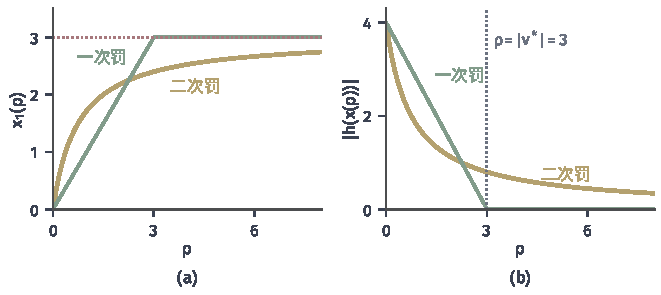
\includegraphics[width=112mm]{figures/05-optimization/06-constrained-optimization/matplotlib/pm-exact-path/figure.pdf}
  \caption{二元例中两种罚函数的解随$\rho$变化。黄线是二次罚，绿线是一次罚，(a)中红色点线是$x_1^\star=3$。(a)第一个坐标：二次罚只能渐近，一次罚在$\rho=3$到达并停住。(b)违规量：一次罚在$\rho\geq3$时恰为零，门槛等于$\lvert\nu^\star\rvert$。}
  \label{fig:pm-exact-path}
\end{BookInlineFigure}

\begin{BookInlineTable}
  \centering
  \begin{tabular}{@{}lll@{}}
    \toprule
     & 二次罚$Q_\rho$ & 一次罚$E_\rho$\\
    \midrule
    边界上的斜率 & 零 & 非零\\
    有限$\rho$的解 & 一般不可行 & 超过门槛后可行\\
    光滑性 & 一阶连续可微 & 边界上不可微\\
    $\rho$的取法 & 必须趋于无穷 & 只需超过乘子门槛\\
    内层困难 & 法向曲率增长 & 解处有尖角\\
    \bottomrule
  \end{tabular}
  \caption{二次罚与一次罚的对照。二次罚以病态换取光滑，一次罚以不可微换取有限的罚参数。}
  \label{tab:pm-penalty-contrast}
\end{BookInlineTable}

\subsection{精确性的条件}
\label{sec:pm-exact-conditions}

门槛和乘子的关系不是例子的巧合。下面要把它写成定理，并分清全局和局部两个层次。

\paragraph{全局精确性}
回忆第~\ref{chap:duality}章的记号。Lagrange函数是
\[
 \mathcal{L}(\bm{x},\bm{\lambda},\bm{\nu})=f(\bm{x})+\sum_{i=1}^m\lambda_ig_i(\bm{x})+\sum_{j=1}^p\nu_jh_j(\bm{x}),
\]
对偶函数$q$是$\mathcal{L}$对$\bm{x}$的下确界。弱对偶说$\bm{\lambda}\geq\bm{0}$时$q(\bm{\lambda},\bm{\nu})\leq f^\star$；强对偶说存在$(\bm{\lambda}^\star,\bm{\nu}^\star)$使等号成立。这个下界和一次罚函数放在一起，就是图~\ref{fig:pm-exact-1d}(b)的画面：$\mathcal{L}(x,\lambda^\star)$是整条水平线，$E_\rho$处处在它上方。

\begin{theorem}[一次罚的全局精确性]
\label{thm:pm-exact-global}
设原问题的最优解$\bm{x}^\star$存在，对偶问题的最优解$(\bm{\lambda}^\star,\bm{\nu}^\star)$存在，且强对偶成立，$q(\bm{\lambda}^\star,\bm{\nu}^\star)=f^\star$。若
\begin{equation}
 \rho>\max\Bigl\{\max_i\lambda_i^\star,\ \max_j\lvert\nu_j^\star\rvert\Bigr\},
 \label{eq:pm-exact-threshold}
\end{equation}
则$E_\rho$的全局最小点集合恰好等于原问题的全局最优解集合，且对所有$\bm{x}$有
\begin{equation}
 E_\rho(\bm{x})\geq f^\star+\delta V(\bm{x}),
 \label{eq:pm-exact-lower-bound}
\end{equation}
其中$\delta>0$是$\rho$与门槛之差。
\end{theorem}

\begin{proof}
记门槛为$\rho_0$，$\delta=\rho-\rho_0>0$。先建立式~\eqref{eq:pm-exact-lower-bound}。由$\lambda_i^\star\geq0$和$g_i\leq[g_i]_+$，有
\[
 \lambda_i^\star g_i(\bm{x})\leq\lambda_i^\star[g_i(\bm{x})]_+\leq\rho_0[g_i(\bm{x})]_+ .
\]
对等式项同样有
\[
 \nu_j^\star h_j(\bm{x})\leq\lvert\nu_j^\star\rvert\lvert h_j(\bm{x})\rvert\leq\rho_0\lvert h_j(\bm{x})\rvert .
\]
把这些不等式对$i,j$求和，得到
\[
 \sum_i\lambda_i^\star g_i(\bm{x})+\sum_j\nu_j^\star h_j(\bm{x})\leq\rho_0V(\bm{x}).
\]

于是
\[
 \begin{aligned}
 E_\rho(\bm{x})&=f(\bm{x})+\rho_0V(\bm{x})+\delta V(\bm{x})\\
 &\geq\mathcal{L}(\bm{x},\bm{\lambda}^\star,\bm{\nu}^\star)+\delta V(\bm{x})\\
 &\geq q(\bm{\lambda}^\star,\bm{\nu}^\star)+\delta V(\bm{x}).
 \end{aligned}
\]
由强对偶，最后一式等于$f^\star+\delta V(\bm{x})$，这就是式~\eqref{eq:pm-exact-lower-bound}。

再看最小点集合。任一原问题最优解$\bm{x}^\star$满足$V(\bm{x}^\star)=0$，$E_\rho(\bm{x}^\star)=f^\star$，由下界知它是$E_\rho$的全局最小点，且$E_\rho$的最小值是$f^\star$。

反过来，设$\bar{\bm{x}}$是$E_\rho$的全局最小点，则$E_\rho(\bar{\bm{x}})=f^\star$。代入下界得$\delta V(\bar{\bm{x}})\leq0$，所以$V(\bar{\bm{x}})=0$，$\bar{\bm{x}}$可行。此时$f(\bar{\bm{x}})=E_\rho(\bar{\bm{x}})=f^\star$，它是原问题的最优解。
\end{proof}

式~\eqref{eq:pm-exact-threshold}中的门槛用的是最大绝对分量，因为总违规量是$\ell_1$形式，两者互为对偶范数。门槛可以按任一组最优乘子计算，最优乘子不唯一时，取能使门槛最小的一组。

证明里没有用到凸性，全部负担都在强对偶上。对一般的非凸问题，强对偶很少成立，所以全局精确性主要是凸问题的结论；第~\ref{chap:duality}章给出的Slater条件是常用的充分条件。

严格不等号也不能省。一维例中$\rho=1$恰好等于门槛，$E_1$的最小点是整条射线$(-\infty,1]$，原问题的解只是其中一点。此时$\delta=0$，下界~\eqref{eq:pm-exact-lower-bound}里违规量的系数消失，最后一步推不出可行。

\paragraph{对偶解不存在时}
去掉“对偶最优解存在”，结论会彻底失败。考虑
\[
 \min_x\ x\qquad\text{s.t.}\qquad x^2\leq0 .
\]
可行集只有$\{0\}$，$x^\star=0$。这是凸问题，$q(\lambda)=-1/(4\lambda)$，$\lambda\to\infty$时趋于$0=f^\star$，但上确界取不到，不存在有限的最优乘子。它的一次罚是$E_\rho(x)=x+\rho x^2$，唯一最小点是
\[
 x_\rho=-\frac{1}{2\rho}\neq0 .
\]
对每个有限的$\rho$，最小点都不可行，$\rho$必须趋于无穷。这里约束的梯度在解处是零，违规量$x^2$在解处光滑，根本没有尖角。可见一次罚的尖角要靠约束的梯度才能起作用。

\paragraph{局部精确性}
非凸问题用不上强对偶，可以只问局部：$\bm{x}^\star$是否是$E_\rho$的局部最小点。局部分析有两条路线。一条看约束集的几何，要求违规量控制到可行集的距离；另一条看KKT条件和曲率。

第一条路线的条件是\term{局部误差界}（local error bound）：存在$\tau>0$和$\bm{x}^\star$的邻域，使邻域内的$\bm{x}$满足
\begin{equation}
 \operatorname{dist}(\bm{x},\bm{C})\leq\tau V(\bm{x}).
 \label{eq:pm-error-bound}
\end{equation}
它的意思是，违规量小就真的离可行集近，不会出现违规量几乎为零、点却还很远的情况。线性约束时误差界在整个空间成立，这是Hoffman界。对光滑约束，它在Mangasarian--Fromovitz约束资格下成立，证明需要用到非线性系统的度量正则性，篇幅较长，这里只使用结论。

第二条路线要用到二阶条件。在KKT点$(\bm{x}^\star,\bm{\lambda}^\star,\bm{\nu}^\star)$处，临界方向$\bm{d}$满足
\begin{equation}
 \nabla h_j(\bm{x}^\star)^\top\bm{d}=0,\qquad
 \begin{cases}
 \nabla g_i(\bm{x}^\star)^\top\bm{d}=0, & g_i(\bm{x}^\star)=0,\ \lambda_i^\star>0,\\
 \nabla g_i(\bm{x}^\star)^\top\bm{d}\leq0, & g_i(\bm{x}^\star)=0,\ \lambda_i^\star=0.
 \end{cases}
 \label{eq:pm-critical-cone}
\end{equation}
二阶充分条件要求Lagrange函数在KKT点处的Hessian沿每个非零临界方向$\bm{d}$都有正曲率：
\[
 \bm{d}^\top\nabla^2_{\bm{x}\bm{x}}\mathcal{L}(\bm{x}^\star,\bm{\lambda}^\star,\bm{\nu}^\star)\bm{d}>0 .
\]
它的含义第~\ref{chap:constrained-optimality}章已经建立。

\begin{theorem}[一次罚的局部精确性]
\label{thm:pm-exact-local}
设$\bm{x}^\star$是可行点。
\begin{enumerate}
 \item 设$\bm{C}$是闭集，$\bm{x}^\star$是$f$在$\bm{C}$上的局部最小点，$f$在$\bm{x}^\star$的邻域内$G$-Lipschitz，且局部误差界~\eqref{eq:pm-error-bound}成立。若$\rho>G\tau$，则$\bm{x}^\star$是$E_\rho$的局部最小点。
 \item 设$f,g_i,h_j$二阶连续可微，$(\bm{x}^\star,\bm{\lambda}^\star,\bm{\nu}^\star)$是KKT点并满足二阶充分条件。若$\rho$满足式~\eqref{eq:pm-exact-threshold}，则$\bm{x}^\star$是$E_\rho$的严格局部最小点。
\end{enumerate}
\end{theorem}

\begin{proof}
先证第一部分。取充分小的$r>0$，使$\lVert\bm{x}-\bm{x}^\star\rVert_2\leq r$时误差界成立，并使$\bm{x}^\star$在半径$2r$的球内是$f$在$\bm{C}$上的最小点，$f$在该球内$G$-Lipschitz。

任取这样的$\bm{x}$，设$\bm{y}$是$\bm{x}$在闭集$\bm{C}$上的一个最近点。$\bm{x}^\star$也在$\bm{C}$中，所以
\[
 \lVert\bm{x}-\bm{y}\rVert_2\leq\lVert\bm{x}-\bm{x}^\star\rVert_2\leq r .
\]
由三角不等式，$\bm{y}$在半径$2r$的球内。于是
\[
 f(\bm{x})\geq f(\bm{y})-G\lVert\bm{x}-\bm{y}\rVert_2\geq f(\bm{x}^\star)-G\tau V(\bm{x}).
\]
由此得
\[
 E_\rho(\bm{x})\geq f(\bm{x}^\star)+(\rho-G\tau)V(\bm{x})\geq E_\rho(\bm{x}^\star).
\]

再证第二部分，用反证法。设$\bm{x}^\star$不是严格局部最小点，则存在$\bm{x}^{(k)}\to\bm{x}^\star$，$\bm{x}^{(k)}\neq\bm{x}^\star$，$E_\rho(\bm{x}^{(k)})\leq f(\bm{x}^\star)$。记$\bm{d}^{(k)}=\bm{x}^{(k)}-\bm{x}^\star$，取子列使单位向量$\bm{d}^{(k)}/\lVert\bm{d}^{(k)}\rVert_2$收敛到$\bm{d}$。

记$\rho_0$为式~\eqref{eq:pm-exact-threshold}的右端，$\delta=\rho-\rho_0>0$，$[a]_-=\max\{-a,0\}$。对单个不等式约束，$a=g_i(\bm{x}^{(k)})$时有
\[
 \rho[a]_+-\lambda_i^\star a\geq\delta[a]_++\lambda_i^\star[a]_- .
\]
这个不等式分两种情形验证：$a>0$时左边等于$(\rho-\lambda_i^\star)a\geq\delta a$，$a\leq0$时左边等于$\lambda_i^\star\lvert a\rvert$。等式项类似，
\[
 \rho\lvert h_j\rvert-\nu_j^\star h_j\geq\delta\lvert h_j\rvert .
\]

把它们加起来，并用$\mathcal{L}^\star$表示乘子固定为$(\bm{\lambda}^\star,\bm{\nu}^\star)$的Lagrange函数，得到
\[
 E_\rho(\bm{x}^{(k)})\geq\mathcal{L}^\star(\bm{x}^{(k)})+\delta V(\bm{x}^{(k)})+\sum_i\lambda_i^\star[g_i(\bm{x}^{(k)})]_- .
\]
KKT条件给出$\mathcal{L}^\star(\bm{x}^\star)=f(\bm{x}^\star)$和$\nabla\mathcal{L}^\star(\bm{x}^\star)=\bm{0}$。作二阶展开，记$\bm{W}=\nabla^2\mathcal{L}^\star(\bm{x}^\star)$，则
\[
 \mathcal{L}^\star(\bm{x}^{(k)})=f(\bm{x}^\star)+\frac12(\bm{d}^{(k)})^\top\bm{W}\bm{d}^{(k)}+o(\lVert\bm{d}^{(k)}\rVert_2^2).
\]
结合$E_\rho(\bm{x}^{(k)})\leq f(\bm{x}^\star)$，得到
\[
 \delta V(\bm{x}^{(k)})+\sum_i\lambda_i^\star[g_i(\bm{x}^{(k)})]_-
 \leq-\frac12(\bm{d}^{(k)})^\top\bm{W}\bm{d}^{(k)}+o(\lVert\bm{d}^{(k)}\rVert_2^2).
\]

右边是$O(\lVert\bm{d}^{(k)}\rVert_2^2)$，所以左边每一项都是这个量级。展开$h_j(\bm{x}^{(k)})$，除以$\lVert\bm{d}^{(k)}\rVert_2$取极限，由$\lvert h_j\rvert=O(\lVert\bm{d}^{(k)}\rVert_2^2)$得$\nabla h_j(\bm{x}^\star)^\top\bm{d}=0$。对活动的$g_i$，$[g_i]_+=O(\lVert\bm{d}^{(k)}\rVert_2^2)$给出$\nabla g_i(\bm{x}^\star)^\top\bm{d}\leq0$；当$\lambda_i^\star>0$时，$[g_i]_-$也是这个量级，于是等号成立。所以$\bm{d}$是非零临界方向。

最后，上式左边非负。两边除以$\lVert\bm{d}^{(k)}\rVert_2^2$取极限，得到$\bm{d}^\top\bm{W}\bm{d}\leq0$，与二阶充分条件矛盾。
\end{proof}

两部分的结论都只说$\bm{x}^\star$附近的事。局部精确不等于全局精确，例如$\min-x^4$，约束$x=0$。此时$\nu^\star=0$，门槛是零，对任何$\rho>0$，$x=0$都是$E_\rho(x)=-x^4+\rho\lvert x\rvert$的严格局部最小点，而$x\to\infty$时$E_\rho\to-\infty$。

\subsection{非光滑罚问题的求解}
\label{sec:pm-exact-solve}

有了精确性，还要回答怎么解$E_\rho$。它的尖角恰好在解的位置上，光滑方法在这里不能直接使用。第~\ref{chap:nonsmooth-composite-optimization}章的工具可以逐一套用，但每种工具都要先核对问题的结构。

\paragraph{次梯度与最优性}
设$f$和$h_j$可微，问题是凸的。$0\in\partial E_\rho(\bm{x})$写开来，就是存在$\xi_j\in\partial\lvert\cdot\rvert(h_j(\bm{x}))$，使
\begin{equation}
 \nabla f(\bm{x})+\sum_{j=1}^p\rho\xi_j\nabla h_j(\bm{x})=\bm{0}.
 \label{eq:pm-exact-subgradient}
\end{equation}
和KKT的驻定方程比较，$\nu_j=\rho\xi_j$就是乘子估计。$\xi_j$落在$[-1,1]$内，$\lvert\nu_j\rvert\leq\rho$。如果解上某条约束的$\lvert\xi_j\rvert=1$且仍然违规，说明罚参数不够大，或者问题本身不可行。

次梯度法只需要这些$\xi_j$，但第~\ref{chap:nonsmooth-composite-optimization}章已经看到，步长固定时点会在尖角附近反复跳动，收敛很慢。图~\ref{fig:pm-exact-ista}里的黄线就是这种行为，它在约束直线两侧来回穿越，几乎每一步都不可行。

\paragraph{邻近梯度}
若把光滑部分$f$留给梯度步，把$\rho V$留给邻近步，就是第~\ref{chap:nonsmooth-composite-optimization}章的邻近梯度法。关键在于邻近映射能否算出。对二元例，设$\bm{a}=(1,1)$，$\tau=\alpha\rho$，要解的子问题是
\begin{equation}
 \bm{p}=\argmin_{\bm{x}}\ \frac12\lVert\bm{x}-\bm{v}\rVert_2^2+\tau\lvert\bm{a}^\top\bm{x}-4\rvert .
 \label{eq:pm-exact-prox}
\end{equation}
由最优性条件，存在$\lvert\cdot\rvert$在$\bm{a}^\top\bm{p}-4$处的次梯度$\xi$，使$\bm{p}=\bm{v}-\tau\xi\bm{a}$。两边与$\bm{a}$作内积，得到
\[
 \bm{a}^\top\bm{p}-4=\bm{a}^\top\bm{v}-4-\tau\xi\lVert\bm{a}\rVert_2^2 .
\]
令$s=(\bm{a}^\top\bm{v}-4)/\lVert\bm{a}\rVert_2^2$。若$\lvert s\rvert\leq\tau$，取$\xi=s/\tau$可使约束恰好满足，这时$\bm{p}$就是$\bm{v}$到直线的投影。若$\lvert s\rvert>\tau$，约束仍然违规，$\xi=\operatorname{sign}(s)$。两种情形合写成
\begin{equation}
 \bm{p}=\bm{v}-\operatorname{clip}_\tau(s)\,\bm{a},\qquad
 \operatorname{clip}_\tau(s)=\max\{-\tau,\min\{s,\tau\}\}.
 \label{eq:pm-exact-prox-solution}
\end{equation}

下面用这个公式走几步。取$\rho=4$，它大于门槛$3$。$f$的光滑常数是$3$，步长$\alpha=1/3$，所以$\tau=4/3$。迭代$\bm{v}=\bm{x}-\alpha\nabla f(\bm{x})$的两个坐标是$\tfrac23x_1$和$0$：
\[
 \bm{v}=\Bigl(x_1-\frac13x_1,\ x_2-x_2\Bigr)=\Bigl(\frac23x_1,\ 0\Bigr).
\]
从$\bm{x}^{(0)}=(0,0)$出发，$\bm{v}=(0,0)$，$s=-2$，被截断到$-\tau$，得到
\[
 \bm{x}^{(1)}=\Bigl(\frac43,\ \frac43\Bigr).
\]
第二步$\bm{v}=(\tfrac89,0)$，$s=-\tfrac{14}{9}$，仍被截断，得到
\[
 \bm{x}^{(2)}=\Bigl(\frac{20}{9},\ \frac43\Bigr).
\]
第三步$\bm{v}=(\tfrac{40}{27},0)$，$s=-\tfrac{34}{27}$，这次$\lvert s\rvert<\tau$，投影到直线上，得到
\[
 \bm{x}^{(3)}=\Bigl(\frac{74}{27},\ \frac{34}{27}\Bigr),\qquad h(\bm{x}^{(3)})=0 .
\]
此后每步都留在直线上，并沿直线逼近$(3,1)$。乘子估计可以从$\nu=\rho\xi=s/\alpha$读出，第三步是$-\tfrac{34}{9}\approx-3.78$，到解处变为$-3$。图~\ref{fig:pm-exact-ista}的绿线就是这条路径：有限步后恰好可行，这是尖角带来的好处，二次罚做不到。

\begin{BookInlineFigure}
  \centering
  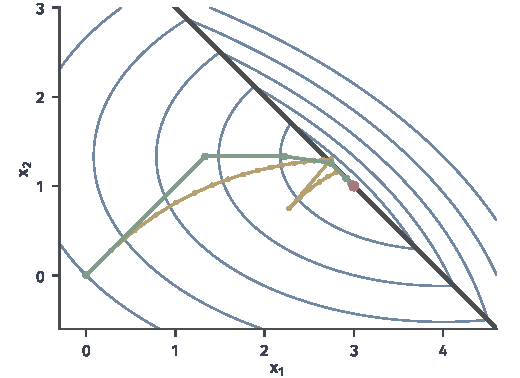
\includegraphics[width=88mm]{figures/05-optimization/06-constrained-optimization/matplotlib/pm-exact-ista/figure.pdf}
  \caption{二元例中一次罚$E_4$的两种解法，蓝线是等高线，深灰直线是约束。绿线是邻近梯度法（步长$1/3$），第三步落到直线上，此后沿直线走向红点。黄线是次梯度法（步长$0.07$），在直线两侧反复穿越，停留在解附近的一个小区域。}
  \label{fig:pm-exact-ista}
\end{BookInlineFigure}

\paragraph{一般约束的处理}
这个闭式解依赖约束只有一条且是线性的。若$\bm{h}(\bm{x})=\bm{A}\bm{x}-\bm{b}$有多行，$\lVert\bm{A}\bm{x}-\bm{b}\rVert_1$的邻近映射本身就要解一个优化问题；若$h_j$非线性，一般没有闭式解。

常用的办法是第~\ref{chap:nonsmooth-composite-optimization}章的局部模型：在当前点把约束线性化，保留绝对值，再加上二次距离项，解
\begin{equation}
 \min_{\bm{d}}\ \nabla f(\bm{x})^\top\bm{d}+\frac{1}{2\alpha}\lVert\bm{d}\rVert_2^2+\rho\sum_{j=1}^p\bigl\lvert h_j(\bm{x})+\nabla h_j(\bm{x})^\top\bm{d}\bigr\rvert .
 \label{eq:pm-exact-model}
\end{equation}
引入非负松弛变量把绝对值拆开，这是一个凸二次规划。模型是否可信要用真实的$E_\rho$检验，也就是比较预测下降和实际下降，第~\ref{chap:sequential-quadratic-programming}章会回到这一点。

解$E_\rho$结束时，还需要回到原问题做两项检查。第一，算出原约束的违规量$V(\bm{x})$，罚目标下降了不代表违规量已经降到容差以下。第二，核对$\rho$是否大于乘子估计的最大绝对分量。如果$\lvert\xi_j\rvert$贴着$1$，定理~\ref{thm:pm-exact-global}的条件就没有满足，应当增大$\rho$再解。数值上的$\rho$也不宜太大，否则目标的信息在罚项面前被淹没，迭代会贴着约束走得很慢。

\section{对偶上升}
\label{sec:pm-dual-ascent}

二次罚的解满足$\rho h(\bm{x}_\rho)\to\nu^\star$，一次罚的门槛也是乘子。两节下来，真正需要的量似乎一直是乘子，罚项只是在间接地把它制造出来。本节换一个问题：如果直接把乘子当作价格来调整，不加任何罚项，能走多远？

\paragraph{价格让碗倾斜}
先回到工厂的例子。总部报出乘子$\nu$，相当于对约束$x_1+x_2-4$计价，两家工厂面对的是Lagrange函数：
\[
 \mathcal{L}(\bm{x},\nu)=\frac12x_1^2+\frac32x_2^2+\nu(x_1+x_2-4).
\]
固定$\nu$，这是一个没有约束的严格凸二次函数。令梯度为零，得到
\begin{equation}
 \bm{x}(\nu)=-\nu\Bigl(1,\ \frac13\Bigr).
 \label{eq:pm-running-lagrange-min}
\end{equation}
写成$p=-\nu$更好读：单价$p$越高，工厂产量越高，$x_1=p$，$x_2=p/3$。线性项$\nu(x_1+x_2)$不改变碗的形状，只把碗底平移。

图~\ref{fig:pm-price-tilt}是平移的过程。$\nu=0$时碗底在原点，离约束很远。$\nu=-2.4$时碗底靠近直线，还差一点。$\nu=-3$时碗底恰好落在约束上的红点处，也就是原问题的解。这时不用任何约束，无约束最小点自己满足了约束。

\begin{BookInlineFigure}
  \centering
  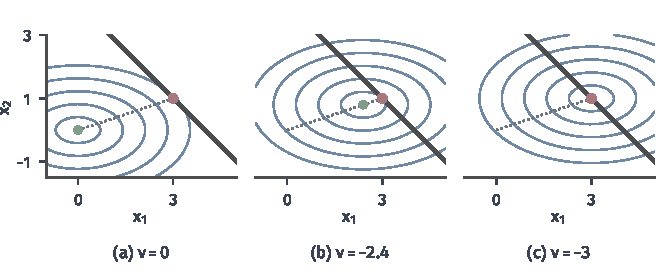
\includegraphics[width=112mm]{figures/05-optimization/06-constrained-optimization/matplotlib/pm-price-tilt/figure.pdf}
  \caption{乘子使Lagrange函数的碗底平移。蓝线是$\mathcal{L}(\cdot,\nu)$的等高线，深灰直线是约束，绿点是$\bm{x}(\nu)$，红点是解$(3,1)$，灰色点线是碗底走过的射线。(c)中$\nu=\nu^\star=-3$，碗底恰好落在约束上。}
  \label{fig:pm-price-tilt}
\end{BookInlineFigure}

把$\bm{x}(\nu)$代回，得到这个例子的对偶函数，它是Lagrange函数在$\bm{x}$上的最小值：
\[
 q(\nu)=\frac12\nu^2+\frac16\nu^2+\nu\Bigl(-\frac43\nu-4\Bigr).
\]
合并同类项，结果是
\begin{equation}
 q(\nu)=-\frac23\nu^2-4\nu .
 \label{eq:pm-running-dual}
\end{equation}
由弱对偶，每个$q(\nu)$都是$f^\star$的下界。这个二次函数在$\nu^\star=-3$处达到最大值$q(-3)=6=f^\star$。

\paragraph{一般情形}
一般问题中，固定$(\bm{\lambda},\bm{\nu})$，要解的是Lagrange子问题。第~\ref{chap:duality}章定义了对偶函数，这里允许把简单的集合$\bm{X}$（如整个空间或盒子）保留在子问题里：
\begin{equation}
 q(\bm{\lambda},\bm{\nu})=\inf_{\bm{x}\in\bm{X}}\mathcal{L}(\bm{x},\bm{\lambda},\bm{\nu}).
 \label{eq:pm-dual-function}
\end{equation}
它是一族关于$(\bm{\lambda},\bm{\nu})$的线性函数的下确界，因此总是凹的，这与原问题是否凸无关。求解对偶问题就是在$\bm{\lambda}\geq\bm{0}$上最大化这个凹函数。

\subsection{残差与乘子更新}
\label{sec:pm-dual-update}

要上升就要知道方向。这里的好消息是：解完Lagrange子问题，约束残差就是现成的上升信息。

\paragraph{残差是超梯度}
二元例的导数是$q'(\nu)=-\tfrac43\nu-4$，把式~\eqref{eq:pm-running-lagrange-min}代入，这恰好等于$h(\bm{x}(\nu))$。一般情形下$q$可能不可微，需要先推广“梯度”。

\begin{definition}[超梯度]
\label{def:pm-supergradient}
设$q$是凹函数，$\bm{y}$是定义域内一点。若向量$\bm{s}$使得对定义域内所有$\bm{y}'$都有
\begin{equation}
 q(\bm{y}')\leq q(\bm{y})+\langle\bm{s},\bm{y}'-\bm{y}\rangle,
 \label{eq:pm-supergradient}
\end{equation}
就称$\bm{s}$是$q$在$\bm{y}$处的\term{超梯度}（supergradient）。
\end{definition}

它就是$-q$的次梯度取负号：凹函数的图形总在这条切线下方。

\begin{theorem}[残差给出超梯度]
\label{thm:pm-residual-supergradient}
设$\bm{\lambda}\geq\bm{0}$，$\bar{\bm{x}}\in\bm{X}$是$\mathcal{L}(\cdot,\bm{\lambda},\bm{\nu})$在$\bm{X}$上的全局最小点。则$(\bm{g}(\bar{\bm{x}}),\bm{h}(\bar{\bm{x}}))$是$q$在$(\bm{\lambda},\bm{\nu})$处的一个超梯度。这里$\bm{g}=(g_1,\ldots,g_m)$，$\bm{h}=(h_1,\ldots,h_p)$，即对所有$\bm{\lambda}'$和$\bm{\nu}'$，有
\begin{equation}
 q(\bm{\lambda}',\bm{\nu}')\leq q(\bm{\lambda},\bm{\nu})+\langle\bm{g}(\bar{\bm{x}}),\bm{\lambda}'-\bm{\lambda}\rangle+\langle\bm{h}(\bar{\bm{x}}),\bm{\nu}'-\bm{\nu}\rangle .
 \label{eq:pm-residual-supergradient}
\end{equation}
\end{theorem}

\begin{proof}
$q$是下确界，所以它不超过任一点上的值：
\[
 q(\bm{\lambda}',\bm{\nu}')\leq\mathcal{L}(\bar{\bm{x}},\bm{\lambda}',\bm{\nu}').
\]
$\mathcal{L}$关于乘子是线性的，把乘子的差分拆出来：
\[
 \mathcal{L}(\bar{\bm{x}},\bm{\lambda}',\bm{\nu}')
 =\mathcal{L}(\bar{\bm{x}},\bm{\lambda},\bm{\nu})+\langle\bm{g}(\bar{\bm{x}}),\bm{\lambda}'-\bm{\lambda}\rangle+\langle\bm{h}(\bar{\bm{x}}),\bm{\nu}'-\bm{\nu}\rangle .
\]
$\bar{\bm{x}}$是全局最小点，所以上式右端第一项等于$q(\bm{\lambda},\bm{\nu})$。代入即得结论。
\end{proof}

证明中只有最后一步用到了最小点，而且必须是全局最小点。若$\bar{\bm{x}}$只是局部最小点，$\mathcal{L}(\bar{\bm{x}},\bm{\lambda},\bm{\nu})$比$q(\bm{\lambda},\bm{\nu})$大，式~\eqref{eq:pm-residual-supergradient}就失去了依据，残差不再是可靠的上升信息。若子问题只解到
\[
 \mathcal{L}(\bar{\bm{x}},\bm{\lambda},\bm{\nu})\leq q(\bm{\lambda},\bm{\nu})+\epsilon,
\]
同样的证明给出多一项$\epsilon$的不等式，$\mathcal{L}(\bar{\bm{x}},\bm{\lambda},\bm{\nu})-\epsilon$仍是可靠的下界。

\paragraph{主要思想}
沿超梯度走一步，不等式乘子投影回非负象限。这就是\term{对偶上升法}（dual ascent）：
\begin{equation}
 \begin{aligned}
 \bm{x}^{(t)}&\in\argmin_{\bm{x}\in\bm{X}}\mathcal{L}(\bm{x},\bm{\lambda}^{(t)},\bm{\nu}^{(t)}),\\
 \bm{\lambda}^{(t+1)}&=\bigl[\bm{\lambda}^{(t)}+\alpha^{(t)}\bm{g}(\bm{x}^{(t)})\bigr]_+,\\
 \bm{\nu}^{(t+1)}&=\bm{\nu}^{(t)}+\alpha^{(t)}\bm{h}(\bm{x}^{(t)}).
 \end{aligned}
 \label{eq:pm-dual-ascent}
\end{equation}
读法和定价一样。某条约束被违反，$g_i>0$，它的价格就上涨；有余量时，价格下降，但不能跌破零。等式约束的价格可正可负，没有截断。

\paragraph{计算过程}
用二元例走一遍，$\bm{X}=\mathbb{R}^2$。

\needspace{6\baselineskip}
\paragraph{变量}
\begin{itemize}
 \item $\bm{\nu}^{(t)}\in\mathbb{R}^p$：当前乘子。例中$p=1$。
 \item $\bm{x}^{(t)}\in\mathbb{R}^n$：Lagrange子问题的解。例中$n=2$。
 \item $\alpha^{(t)}>0$：乘子步长。
\end{itemize}

\paragraph{初始化}
取$\bm{\nu}^{(0)}$和步长。例中$\nu^{(0)}=0$，步长固定为$\alpha=0.6$，结束容差$\varepsilon=0.05$。

\needspace{6\baselineskip}
\paragraph{每轮更新}
\begin{enumerate}
 \item 解Lagrange子问题。例中用式~\eqref{eq:pm-running-lagrange-min}，第一轮
 \[
  \bm{x}^{(0)}=(0,0).
 \]
 \item 计算残差。例中第一轮
 \[
  h(\bm{x}^{(0)})=-4 .
 \]
 \item 按式~\eqref{eq:pm-dual-ascent}更新乘子。例中第一轮
 \[
  \nu^{(1)}=0+0.6\times(-4)=-2.4 .
 \]
\end{enumerate}
第二轮得到
\[
 \bm{x}^{(1)}=(2.4,\ 0.8),\qquad h(\bm{x}^{(1)})=-0.8,\qquad \nu^{(2)}=-2.88 .
\]
第三轮得到
\[
 \bm{x}^{(2)}=(2.88,\ 0.96),\qquad h(\bm{x}^{(2)})=-0.16,\qquad \nu^{(3)}=-2.976 .
\]
第四轮得到
\[
 \bm{x}^{(3)}=(2.976,\ 0.992),\qquad h(\bm{x}^{(3)})=-0.032 .
\]

结束条件是残差不超过$\varepsilon$，例中第四轮满足。最终得到的点是$\bm{x}^{(3)}=(2.976,\ 0.992)$，四轮对应的下界依次是
\[
 q(\nu^{(0)})=0,\quad q(\nu^{(1)})=5.76,\quad q(\nu^{(2)})=5.9904,\quad q(\nu^{(3)})\approx5.9996,
\]
单调升向$f^\star=6$。但是每一轮的$\bm{x}^{(t)}$都不可行。对偶上升改进的是下界，不是可行性。

\paragraph{步长的范围}
每轮更新代入后可以写成闭式。把$h(\bm{x}(\nu))=-\tfrac43\nu-4$代入，
\[
 \nu^{(t+1)}+3=\Bigl(1-\frac43\alpha\Bigr)(\nu^{(t)}+3).
\]
因此收敛当且仅当$\lvert1-\tfrac43\alpha\rvert<1$，也就是$0<\alpha<\tfrac32$。

图~\ref{fig:pm-dual-ascent}比较两个步长。$\alpha=0.6$时压缩因子是$0.2$，一步比一步接近顶点。$\alpha=1.5$恰好在边界上，因子是$-1$：乘子在$0$和$-6$之间永远跳动，$\bm{x}$在$(0,0)$和$(6,2)$之间跳动，两个点都不可行。

\begin{BookInlineFigure}
  \centering
  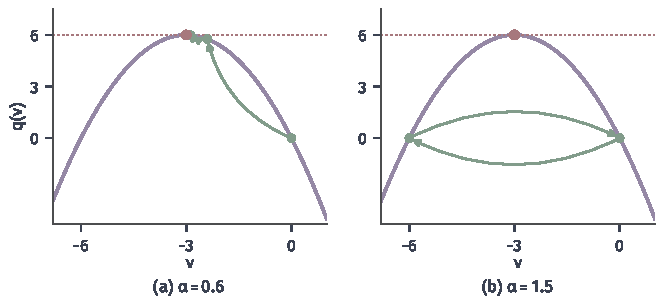
\includegraphics[width=112mm]{figures/05-optimization/06-constrained-optimization/matplotlib/pm-dual-ascent/figure.pdf}
  \caption{二元例中对偶函数$q(\nu)$（紫）上的对偶上升。绿点和箭头是乘子序列，从$\nu^{(0)}=0$出发，红点是最大点，红色点线是$f^\star=6$。(a)$\alpha=0.6$：压缩因子$0.2$，很快接近最大点。(b)$\alpha=1.5$：在$0$与$-6$之间反复跳动，不收敛。}
  \label{fig:pm-dual-ascent}
\end{BookInlineFigure}

\paragraph{可微的情形}
例子中的$q$是光滑的，这并非偶然。当$f$强凸、约束仿射时，子问题的解唯一，超梯度也唯一，对偶函数可以用第~\ref{chap:smooth-foundations}章的光滑分析。

\begin{theorem}[强凸目标的光滑对偶]
\label{thm:pm-smooth-dual}
设$f$连续可微且$\mu$强凸，$\bm{X}=\mathbb{R}^n$，约束为$\bm{A}\bm{x}=\bm{b}$。记$\bm{x}(\bm{\nu})$为$\mathcal{L}(\cdot,\bm{\nu})$的唯一最小点。则$q$可微，并且
\begin{equation}
 \nabla q(\bm{\nu})=\bm{A}\bm{x}(\bm{\nu})-\bm{b},
 \label{eq:pm-smooth-dual}
\end{equation}
其梯度满足
\begin{equation}
 \lVert\nabla q(\bm{\nu}_1)-\nabla q(\bm{\nu}_2)\rVert_2\leq\frac{\lVert\bm{A}\rVert_2^2}{\mu}\lVert\bm{\nu}_1-\bm{\nu}_2\rVert_2 .
 \label{eq:pm-smooth-dual-lipschitz}
\end{equation}
于是只要最优乘子存在，固定步长$0<\alpha<2\mu/\lVert\bm{A}\rVert_2^2$的对偶上升满足$q(\bm{\nu}^{(t)})\to d^\star$，其中$d^\star$是对偶最优值。
\end{theorem}

\begin{proof}
记$\bm{x}_k=\bm{x}(\bm{\nu}_k)$。驻定条件给出$\nabla f(\bm{x}_k)=-\bm{A}^\top\bm{\nu}_k$。由强凸性，
\[
 \mu\lVert\bm{x}_1-\bm{x}_2\rVert_2^2\leq\langle\nabla f(\bm{x}_1)-\nabla f(\bm{x}_2),\bm{x}_1-\bm{x}_2\rangle .
\]
把驻定条件代入，并用Cauchy--Schwarz不等式，得到
\[
 \mu\lVert\bm{x}_1-\bm{x}_2\rVert_2^2
 \leq-\langle\bm{\nu}_1-\bm{\nu}_2,\bm{A}(\bm{x}_1-\bm{x}_2)\rangle
 \leq\lVert\bm{A}\rVert_2\lVert\bm{\nu}_1-\bm{\nu}_2\rVert_2\lVert\bm{x}_1-\bm{x}_2\rVert_2 .
\]
两边约去一个因子，得到
\[
 \lVert\bm{x}_1-\bm{x}_2\rVert_2\leq\frac{\lVert\bm{A}\rVert_2}{\mu}\lVert\bm{\nu}_1-\bm{\nu}_2\rVert_2 .
\]

记$\bm{s}(\bm{\nu})=\bm{A}\bm{x}(\bm{\nu})-\bm{b}$。由上式，$\bm{s}$满足式~\eqref{eq:pm-smooth-dual-lipschitz}的Lipschitz界。

由定理~\ref{thm:pm-residual-supergradient}，$\bm{s}(\bm{\nu}_1)$和$\bm{s}(\bm{\nu}_2)$分别是两点的超梯度。对两点分别写一次超梯度不等式，得到
\[
 \langle\bm{s}(\bm{\nu}_2),\bm{\nu}_2-\bm{\nu}_1\rangle\leq q(\bm{\nu}_2)-q(\bm{\nu}_1)\leq\langle\bm{s}(\bm{\nu}_1),\bm{\nu}_2-\bm{\nu}_1\rangle .
\]
上下两端相差不超过$\lVert\bm{s}(\bm{\nu}_2)-\bm{s}(\bm{\nu}_1)\rVert_2\lVert\bm{\nu}_2-\bm{\nu}_1\rVert_2$，这是$\lVert\bm{\nu}_2-\bm{\nu}_1\rVert_2$的二阶量，所以$q$在$\bm{\nu}_1$处可微，梯度是$\bm{s}(\bm{\nu}_1)$。

最后，$-q$是光滑凸函数，步长范围内的梯度法收敛结论见第~\ref{chap:smooth-foundations}章和第~\ref{chap:first-order-methods}章。
\end{proof}

在二元例中，$\bm{A}=(1,1)$，$\lVert\bm{A}\rVert_2^2=2$，$f$的强凸常数$\mu=1$，定理的步长上限是$1$，比实际范围$\tfrac32$保守。这是因为定理把两个坐标方向的曲率都按最小值$\mu=1$估计，而实际的$\lvert q''\rvert$只有$\tfrac43$。

\paragraph{不可微的情形}
$f$不强凸时，子问题的解可能不唯一，$q$在这些点上有折角。下面的例子有两个变量和一条资源约束，后面还要继续使用：
\begin{equation}
 \min_{\bm{x}\in[0,1]^2}\ -x_1-x_2\qquad\text{s.t.}\qquad 2x_1+2x_2\leq3 .
 \label{eq:pm-lp-resource}
\end{equation}
它的最优值$f^\star=-1.5$，在$x_1+x_2=1.5$的线段上取得。固定$\lambda\geq0$，子问题对两个变量是分开的线性函数，每个变量的系数是$2\lambda-1$。

因此$\lambda<\tfrac12$时解是$(1,1)$，$\lambda>\tfrac12$时解是$(0,0)$，$\lambda=\tfrac12$时任意点都是解。代入得到对偶函数：
\[
 q(\lambda)=\begin{cases}\lambda-2,&\lambda\leq\tfrac12,\\-3\lambda,&\lambda\geq\tfrac12.\end{cases}
\]
$q$在$\lambda^\star=\tfrac12$处达到最大值$-1.5$，折角正好在最优点上。

超梯度步未必提高$q$。取$\alpha=0.12$，$\lambda^{(0)}=0$，乘子序列是
\[
 0,\ 0.12,\ 0.24,\ 0.36,\ 0.48,\ 0.60,\ 0.24,\ 0.36,\ 0.48,\ 0.60,\ldots
\]
对偶值$q(0.48)=-1.52$，下一步$q(0.60)=-1.8$，反而下降了。这与第~\ref{chap:nonsmooth-composite-optimization}章的次梯度法一样：步子越过折角就会下降，能保证的是到最优乘子的距离或者最好点的对偶值，而不是每步上升。图~\ref{fig:pm-primal-recovery}(a)中的绿点就在折角两侧来回。

\subsection{对偶分解与原始恢复}
\label{sec:pm-decomposition}

这一小节回答两个问题：对偶上升的计算好在哪里，以及算到最后怎样得到一个能用的原始解。

\paragraph{固定价格后各块分离}
设变量分成$K$块，目标按块可分，只有一条线性资源约束把它们联系起来：
\begin{equation}
 \min_{\bm{x}_k\in\bm{X}_k}\ \sum_{k=1}^Kf_k(\bm{x}_k)\qquad\text{s.t.}\qquad\sum_{k=1}^K\bm{A}_k\bm{x}_k\leq\bm{b}.
 \label{eq:pm-separable}
\end{equation}
固定乘子$\bm{\lambda}\geq\bm{0}$，Lagrange函数按块拆开：
\[
 \mathcal{L}(\bm{x},\bm{\lambda})=\sum_{k=1}^K\Bigl(f_k(\bm{x}_k)+\langle\bm{\lambda},\bm{A}_k\bm{x}_k\rangle\Bigr)-\langle\bm{\lambda},\bm{b}\rangle .
\]
和式中的每一项只含一块变量，所以$K$个子问题可以独立求解，互不通信。这种做法称为\term{对偶分解}（dual decomposition）。

协调者只做一件事：收集各块的用量$\bm{A}_k\bm{x}_k$，算出总残差，按下式更新价格：
\begin{equation}
 \bm{\lambda}^{(t+1)}=\Bigl[\bm{\lambda}^{(t)}+\alpha^{(t)}\Bigl(\sum_{k=1}^K\bm{A}_k\bm{x}_k^{(t)}-\bm{b}\Bigr)\Bigr]_+ .
 \label{eq:pm-decomposition-update}
\end{equation}
图~\ref{fig:pm-decomposition}以二元例为例，它本身就是两块问题：每家工厂只知道自己的成本和价格，协调者只知道总量和目标。

\begin{BookInlineFigure}
  \centering
  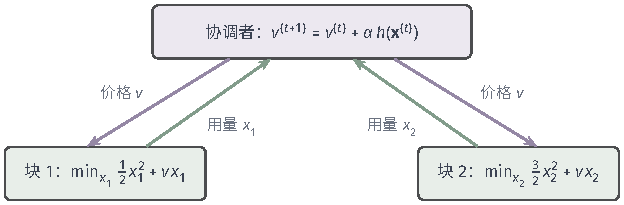
\includegraphics[width=105mm]{figures/05-optimization/06-constrained-optimization/tikz/pm-decomposition/figure.pdf}
  \caption{二元例的对偶分解。协调者（紫框）把当前价格$\nu$发给各块（紫色箭头），两块（绿框）独立求解自己的子问题，再把用量报回（绿色箭头）。协调者只用总量更新价格，不需要知道各块的成本函数。}
  \label{fig:pm-decomposition}
\end{BookInlineFigure}

分解改变的是计算的组织方式，算法在数学上仍是同一个对偶上升。收敛性质不因为分块而变好，第~\ref{chap:block-optimization}章处理的是目标本身不可分的分块，这里的分块靠乘子把约束解开。

\paragraph{原始点不可行}
继续看式~\eqref{eq:pm-lp-resource}。两个变量的子问题总是给出$(1,1)$或$(0,0)$。前者违反资源约束，$2x_1+2x_2=4>3$；后者可行，目标值却是$0$，离$f^\star$很远。图~\ref{fig:pm-primal-recovery}(b)的绿线就是这种情况：总量$x_1+x_2$一直在$2$和$0$之间跳，从不等于最优所需的$1.5$。

原因在于，对偶上升求的是价格，给定价格之后，解可以停在子问题解集的任何一点上。这个例子里，$\lambda^\star=\tfrac12$处的子问题有无穷多解，$q$的最大点却完全不告诉我们选哪个。

\paragraph{平均恢复}
第~\ref{chap:nonsmooth-composite-optimization}章在次梯度法上用过的平均，这里有直接的物理含义。把$\lambda$上涨的轮次看成资源用多了，下跌的轮次看成用少了，平均之后用量大致等于资源总量。图~\ref{fig:pm-primal-recovery}(b)的黄线是$x_1^{(t)}+x_2^{(t)}$的累积平均，它趋于$1.5$。

\begin{BookInlineFigure}
  \centering
  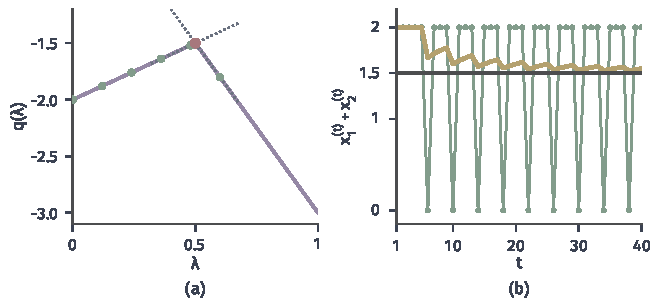
\includegraphics[width=112mm]{figures/05-optimization/06-constrained-optimization/matplotlib/pm-primal-recovery/figure.pdf}
  \caption{资源问题的超梯度上升，$\alpha=0.12$。(a)紫线是对偶函数，折角在$\lambda^\star=\tfrac12$，灰色点线是折角处的两条支撑线，绿点是前九个乘子，红点是最大点。(b)绿线是每轮的总量$x_1^{(t)}+x_2^{(t)}$，在$2$与$0$之间跳动；黄线是累积平均，深灰线是$1.5$。}
  \label{fig:pm-primal-recovery}
\end{BookInlineFigure}

\begin{theorem}[平均点的可行性与目标]
\label{thm:pm-primal-average}
设$f$和$g_i$在非空紧凸集$\bm{X}$上凸且连续，问题只有不等式约束，$f^\star$有限。设$\lVert\bm{g}(\bm{x})\rVert_2\leq S$对$\bm{x}\in\bm{X}$成立。从$\bm{\lambda}^{(0)}\geq\bm{0}$出发，取固定步长$\alpha>0$运行式~\eqref{eq:pm-dual-ascent}。记$\bar{\bm{x}}^{(T)}$为$\bm{x}^{(0)},\ldots,\bm{x}^{(T-1)}$的算术平均，则平均点在$\bm{X}$内，并且
\begin{equation}
 \bm{g}(\bar{\bm{x}}^{(T)})\leq\frac{\bm{\lambda}^{(T)}}{\alpha T},
 \label{eq:pm-average-feasibility}
\end{equation}
\begin{equation}
 f(\bar{\bm{x}}^{(T)})-f^\star\leq\frac{\lVert\bm{\lambda}^{(0)}\rVert_2^2}{2\alpha T}+\frac{\alpha S^2}{2}.
 \label{eq:pm-average-objective}
\end{equation}
\end{theorem}

\begin{proof}
先证可行性。投影只会让乘子变大，$[a]_+\geq a$，所以
\[
 \bm{\lambda}^{(t+1)}\geq\bm{\lambda}^{(t)}+\alpha\bm{g}(\bm{x}^{(t)}).
\]
对$t=0,\ldots,T-1$求和，得到
\[
 \alpha\sum_{t=0}^{T-1}\bm{g}(\bm{x}^{(t)})\leq\bm{\lambda}^{(T)}-\bm{\lambda}^{(0)}\leq\bm{\lambda}^{(T)}.
\]
每个$g_i$是凸函数，由Jensen不等式，平均点上的函数值不超过函数值的平均：
\[
 g_i(\bar{\bm{x}}^{(T)})\leq\frac1T\sum_{t=0}^{T-1}g_i(\bm{x}^{(t)}).
\]
两式结合，除以$\alpha T$，即得式~\eqref{eq:pm-average-feasibility}。

再证目标。投影到非负象限不增加与原点的距离，所以
\[
 \lVert\bm{\lambda}^{(t+1)}\rVert_2^2\leq\lVert\bm{\lambda}^{(t)}+\alpha\bm{g}(\bm{x}^{(t)})\rVert_2^2\leq\lVert\bm{\lambda}^{(t)}\rVert_2^2+2\alpha\langle\bm{\lambda}^{(t)},\bm{g}(\bm{x}^{(t)})\rangle+\alpha^2S^2 .
\]
由弱对偶和$\bm{x}^{(t)}$的定义，
\[
 f(\bm{x}^{(t)})+\langle\bm{\lambda}^{(t)},\bm{g}(\bm{x}^{(t)})\rangle=q(\bm{\lambda}^{(t)})\leq f^\star .
\]
从上式解出内积，代入前一个不等式，得到
\[
 f(\bm{x}^{(t)})-f^\star\leq\frac{\lVert\bm{\lambda}^{(t)}\rVert_2^2-\lVert\bm{\lambda}^{(t+1)}\rVert_2^2}{2\alpha}+\frac{\alpha S^2}{2}.
\]
对$t$求和，左边用Jensen不等式，右边裂项相消，去掉非正的$-\lVert\bm{\lambda}^{(T)}\rVert_2^2$，除以$T$即得式~\eqref{eq:pm-average-objective}。
\end{proof}

平均点的违规量由$\bm{\lambda}^{(T)}/(\alpha T)$控制，只要乘子序列有界，它就以$1/T$趋于零。Slater条件可以保证有界。设$\tilde{\bm{x}}\in\bm{X}$满足$g_i(\tilde{\bm{x}})\leq-\sigma<0$，并记$f_{\min}$为$f$在$\bm{X}$上的最小值。对偶函数不超过$\mathcal{L}$在$\tilde{\bm{x}}$处的值，由此得到
\[
 \langle\bm{\lambda}^{(t)},\bm{g}(\bm{x}^{(t)})\rangle=q(\bm{\lambda}^{(t)})-f(\bm{x}^{(t)})\leq f(\tilde{\bm{x}})-f_{\min}-\sigma\lVert\bm{\lambda}^{(t)}\rVert_1 .
\]
记
\[
 R=\frac{f(\tilde{\bm{x}})-f_{\min}+\alpha S^2/2}{\sigma}.
\]
代入证明中的距离递推可知，只要$\lVert\bm{\lambda}^{(t)}\rVert_1\geq R$，范数就不会增大；否则一步至多增加$\alpha S$。所以
\[
 \lVert\bm{\lambda}^{(t)}\rVert_2\leq\max\bigl\{\lVert\bm{\lambda}^{(0)}\rVert_2,\ R+\alpha S\bigr\}.
\]

式~\eqref{eq:pm-average-objective}只是单侧的界：$\bar{\bm{x}}^{(T)}$略微不可行时，目标值可能低于$f^\star$。

在问题~\eqref{eq:pm-lp-resource}中，乘子进入周期后每四轮有三轮是$(1,1)$，一轮是$(0,0)$，平均趋于$(\tfrac34,\tfrac34)$，$2x_1+2x_2$趋于$3$，恰好用尽资源。这组权重$\tfrac34,\tfrac14$是从对偶迭代的频率里读出来的，并没有事先知道。

\paragraph{非凸时的恢复与证书}
平均依赖可行集和目标的凸性。把式~\eqref{eq:pm-lp-resource}的变量改成$x_i\in\{0,1\}$，子问题和对偶函数都不变，最优乘子仍是$\tfrac12$，下界最多是$-1.5$。可平均点$(\tfrac34,\tfrac34)$不是整数点，平均在这里没有意义。

这时可以从访问过的点里挑选，或者另加一个简单的修复步骤，例如按边际价值贪心地放入物品，直到资源用尽。这里贪心得到$(1,0)$，目标值$-1$，可行。

此时的结论要如实报告：可行解给出上界$-1$，迭代中最好的对偶值给出下界$-1.52$，间隙不超过$0.52$。这个问题真实的最优值是$-1$，对偶下界不紧是非凸问题的常态，第~\ref{chap:duality}章称之为对偶间隙。任何情况下都应当同时报告原始可行性和这个间隙，单独一个收敛的对偶值不构成原问题的解。

\section{增广Lagrange法（ALM）}
\label{sec:pm-alm}

前面两条路各有缺陷。二次罚能增加法向曲率，把子问题变成好解的碗，但违规量要靠$\rho\to\infty$才能消失。对偶上升不增加任何曲率，步长稍大就振荡，目标线性时子问题甚至定不出解。把价格和罚款放在同一个函数里，能否在有限的$\rho$下得到解？

\paragraph{从力的平衡出发}
二次罚的驻点满足$\nabla f+\rho\bm{J}^\top\bm{h}=\bm{0}$。要平衡目标的力，$\rho\bm{h}$必须接近$\bm{\nu}^\star$，所以$\bm{h}$不能为零。如果事先在罚项里加上一个估计的力$\bm{\nu}$，那么只要$\bm{\nu}$足够接近$\bm{\nu}^\star$，弹簧几乎不用拉长。

工厂的语言是，总部既标出单价，又对偏离总量收罚款。单价负责提供大部分的调节力，罚款只负责修正单价还没估准的那一小部分。写成函数，就是在Lagrange函数上加残差平方。

\begin{definition}[增广Lagrange函数]
\label{def:pm-al}
对等式约束问题和$\rho>0$，\term{增广Lagrange函数}（augmented Lagrangian）是
\begin{equation}
 \mathcal{L}_\rho(\bm{x},\bm{\nu})=f(\bm{x})+\langle\bm{\nu},\bm{h}(\bm{x})\rangle+\frac{\rho}{2}\lVert\bm{h}(\bm{x})\rVert_2^2 .
 \label{eq:pm-al}
\end{equation}
\end{definition}

配方之后可以看出它的结构：
\begin{equation}
 \mathcal{L}_\rho(\bm{x},\bm{\nu})=f(\bm{x})+\frac{\rho}{2}\Bigl\lVert\bm{h}(\bm{x})+\frac{\bm{\nu}}{\rho}\Bigr\rVert_2^2-\frac{1}{2\rho}\lVert\bm{\nu}\rVert_2^2 .
 \label{eq:pm-al-square}
\end{equation}
最后一项与$\bm{x}$无关。所以固定$\bm{\nu}$时，增广Lagrange函数就是一个目标移位的二次罚：它不再要求$\bm{h}=\bm{0}$，而是把残差往$-\bm{\nu}/\rho$处拉。移位量选得对，平衡点上的残差就恰好是零。

\paragraph{同一个例子}
对二元例，固定$\nu$和$\rho$，增广Lagrange函数的驻定方程是
\[
 (1+\rho)x_1+\rho x_2=4\rho-\nu,\qquad \rho x_1+(3+\rho)x_2=4\rho-\nu .
\]
两式相减仍得$x_1=3x_2$。代回得到
\begin{equation}
 x_2=\frac{4\rho-\nu}{3+4\rho},\qquad x_1=3x_2 .
 \label{eq:pm-running-al-solution}
\end{equation}
残差因此是
\begin{equation}
 h(\bm{x})=4x_2-4=-\frac{4(\nu+3)}{3+4\rho}.
 \label{eq:pm-running-al-residual}
\end{equation}
和二次罚的式~\eqref{eq:pm-running-penalty-residual}比较，二次罚对应$\nu=0$，残差只能靠分母变大。这里分子含有因子$\nu-\nu^\star=\nu+3$：只要$\nu=-3$，无论$\rho$多小，残差都是零。

图~\ref{fig:pm-alm-center}固定$\rho=1.5$，只改变$\nu$。等高线的形状完全不变，因为Hessian不依赖$\nu$；变的是碗底的位置，$\nu=0$时离直线较远，$\nu=-2$时贴近直线，$\nu=-3$时恰好落在解上。对比图~\ref{fig:pm-penalty-contours}，那里要靠压扁碗才能靠近直线，这里碗的形状没有变。

\begin{BookInlineFigure}
  \centering
  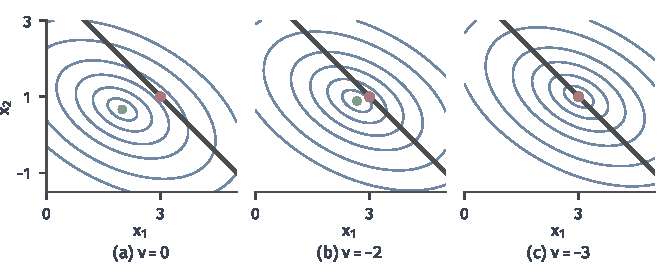
\includegraphics[width=112mm]{figures/05-optimization/06-constrained-optimization/matplotlib/pm-alm-center/figure.pdf}
  \caption{二元例中$\mathcal{L}_{1.5}(\cdot,\nu)$的等高线（蓝），$\rho=1.5$固定。深灰直线是约束，绿点是增广函数的最小点，红点是解$(3,1)$。改变乘子只平移碗底，不改变碗的形状；(c)$\nu=\nu^\star$时最小点落在解上。}
  \label{fig:pm-alm-center}
\end{BookInlineFigure}

这种现象不只在二次例子里出现，它在局部有一般的解释。下面的定理说，只要乘子是对的，有限的$\rho$就够了。

\begin{theorem}[最优乘子下的局部精确性]
\label{thm:pm-al-exact}
设$f,h_j$二阶连续可微，$(\bm{x}^\star,\bm{\nu}^\star)$满足KKT条件。记$\bm{W}$为$\mathcal{L}(\cdot,\bm{\nu}^\star)$在$\bm{x}^\star$处的Hessian，$\bm{J}=\bm{J}(\bm{x}^\star)$，并设对所有非零$\bm{d}$，只要$\bm{J}\bm{d}=\bm{0}$，就有$\bm{d}^\top\bm{W}\bm{d}>0$。则存在$\bar\rho\geq0$，使$\rho>\bar\rho$时，$\bm{x}^\star$是$\mathcal{L}_\rho(\cdot,\bm{\nu}^\star)$的严格局部最小点。
\end{theorem}

\begin{proof}
由$\bm{h}(\bm{x}^\star)=\bm{0}$和KKT条件，
\[
 \nabla_{\bm{x}}\mathcal{L}_\rho(\bm{x}^\star,\bm{\nu}^\star)=\nabla f+\bm{J}^\top\bm{\nu}^\star+\rho\bm{J}^\top\bm{h}=\bm{0}.
\]
含$h_j\nabla^2h_j$的项在$\bm{x}^\star$处为零，所以Hessian是
\[
 \nabla^2_{\bm{x}\bm{x}}\mathcal{L}_\rho(\bm{x}^\star,\bm{\nu}^\star)=\bm{W}+\rho\bm{J}^\top\bm{J}.
\]
只需证明$\rho$足够大时它正定。$\bm{J}^\top\bm{J}$半正定，这个矩阵关于$\rho$是单调的，一旦正定，更大的$\rho$也正定。

用反证法。若对每个正整数$k$，$\bm{W}+k\bm{J}^\top\bm{J}$都不正定，则存在单位向量$\bm{u}_k$，使
\[
 \bm{u}_k^\top\bm{W}\bm{u}_k+k\lVert\bm{J}\bm{u}_k\rVert_2^2\leq0 .
\]
单位向量的序列有收敛子列，设极限为$\bm{u}$。由上式得
\[
 \lVert\bm{J}\bm{u}_k\rVert_2^2\leq\frac{\lVert\bm{W}\rVert_2}{k}\to0 ,
\]
故$\bm{J}\bm{u}=\bm{0}$。

不等式的第二项非负，去掉它得$\bm{u}_k^\top\bm{W}\bm{u}_k\leq0$，取极限得$\bm{u}^\top\bm{W}\bm{u}\leq0$。这与假设矛盾，因为$\bm{u}\neq\bm{0}$且$\bm{J}\bm{u}=\bm{0}$。
\end{proof}

条件中$\bar\rho$的作用，看一个非凸的例子。取$f(\bm{x})=\tfrac12(x_1^2-x_2^2)$，$h(\bm{x})=x_2$，解是原点，$\nu^\star=0$。切方向是$x_1$轴，曲率$1>0$，满足二阶条件。此时增广函数的Hessian是$\operatorname{diag}(1,\rho-1)$，必须$\rho>1$才正定。$\rho<1$时，增广函数沿$x_2$方向没有下界。若$f$是凸函数且约束是线性的，就不需要这个门槛，任何$\rho>0$都行。

\subsection{原始变量与乘子更新}
\label{sec:pm-alm-update}

问题转到怎样得到正确的乘子。上一节的定理给了线索：用$\bm{\nu}$算出的增广函数的驻点，本身就告诉我们乘子该往哪里改。

\paragraph{主要思想}
对$\mathcal{L}_\rho$求梯度，把含$\bm{h}$的项合并，得到一个恒等式：
\begin{equation}
 \nabla_{\bm{x}}\mathcal{L}_\rho(\bm{x},\bm{\nu})=\nabla f(\bm{x})+\bm{J}(\bm{x})^\top\bigl(\bm{\nu}+\rho\bm{h}(\bm{x})\bigr)=\nabla_{\bm{x}}\mathcal{L}\bigl(\bm{x},\bm{\nu}+\rho\bm{h}(\bm{x})\bigr).
 \label{eq:pm-al-gradient-identity}
\end{equation}
如果$\bm{x}^{(t+1)}$是增广函数的驻点，那么它对应的Lagrange函数在乘子$\bm{\nu}^{(t)}+\rho\bm{h}(\bm{x}^{(t+1)})$处驻定。这个乘子把目标的力和约束的力平衡起来了，正好作为新的估计。

由此得到\term{增广Lagrange法}（augmented Lagrangian method，ALM）：
\begin{equation}
 \begin{aligned}
 \bm{x}^{(t+1)}&\approx\argmin_{\bm{x}}\mathcal{L}_{\rho}(\bm{x},\bm{\nu}^{(t)}),\\
 \bm{\nu}^{(t+1)}&=\bm{\nu}^{(t)}+\rho\,\bm{h}(\bm{x}^{(t+1)}).
 \end{aligned}
 \label{eq:pm-alm}
\end{equation}
这里$\rho$既是罚参数，也是乘子的步长。把步长取成$\rho$，正是恒等式~\eqref{eq:pm-al-gradient-identity}选出来的，不是任意的约定。

形式上它和对偶上升~\eqref{eq:pm-dual-ascent}只差一点：残差的取法。对偶上升先在旧乘子下解Lagrange子问题，用得到的残差算新乘子。ALM的$\bm{x}^{(t+1)}$满足的是新乘子下的驻定条件，残差实际上是在“走到之后的乘子”处读的。这正是第~\ref{chap:nonsmooth-composite-optimization}章显式步和隐式步的区别。

\begin{theorem}[ALM是对偶问题的邻近点法]
\label{thm:pm-alm-proximal}
设$f$是适当、闭的凸函数，$\bm{h}(\bm{x})=\bm{A}\bm{x}-\bm{b}$。设$\bm{x}^{+}$是$\mathcal{L}_\rho(\cdot,\bm{\nu})$的全局最小点，$\bm{\nu}^{+}=\bm{\nu}+\rho\bm{h}(\bm{x}^{+})$。则$\bm{x}^{+}$是$\mathcal{L}(\cdot,\bm{\nu}^{+})$的全局最小点，并且
\begin{equation}
 \bm{\nu}^{+}=\bm{\nu}+\rho\bm{s}^{+},\qquad \bm{s}^{+}=\bm{h}(\bm{x}^{+})\text{是}q\text{在}\bm{\nu}^{+}\text{处的超梯度},
 \label{eq:pm-alm-implicit}
\end{equation}
等价地，$\bm{\nu}^{+}$是下面问题的唯一解：
\begin{equation}
 \bm{\nu}^{+}=\argmax_{\bm{y}}\Bigl\{q(\bm{y})-\frac{1}{2\rho}\lVert\bm{y}-\bm{\nu}\rVert_2^2\Bigr\}.
 \label{eq:pm-alm-prox}
\end{equation}
\end{theorem}

\begin{proof}
$\bm{x}^{+}$最小化凸函数$\mathcal{L}_\rho(\cdot,\bm{\nu})$，最优性条件是
\[
 \bm{0}\in\partial f(\bm{x}^{+})+\bm{A}^\top\bigl(\bm{\nu}+\rho(\bm{A}\bm{x}^{+}-\bm{b})\bigr)=\partial f(\bm{x}^{+})+\bm{A}^\top\bm{\nu}^{+}.
\]
这正是凸函数$\mathcal{L}(\cdot,\bm{\nu}^{+})$在$\bm{x}^{+}$处的最优性条件，第一个结论成立。

由定理~\ref{thm:pm-residual-supergradient}，$\bm{s}^{+}=\bm{h}(\bm{x}^{+})$是$q$在$\bm{\nu}^{+}$处的超梯度，再由$\bm{\nu}^{+}$的定义得式~\eqref{eq:pm-alm-implicit}。

式~\eqref{eq:pm-alm-prox}中的目标强凹。它在$\bm{\nu}^{+}$处的最优性条件是$\bm{0}$属于$\partial q(\bm{\nu}^{+})-(\bm{\nu}^{+}-\bm{\nu})/\rho$，而式~\eqref{eq:pm-alm-implicit}正好给出这样一个超梯度。
\end{proof}

图~\ref{fig:pm-explicit-implicit}在二元例上比较两种步。$\rho=1.5$，从$\nu^{(0)}=0$出发，$q$的斜率是$-4$。显式步用当前点的斜率，走到$0+1.5\times(-4)=-6$，越过最大点，这就是图~\ref{fig:pm-dual-ascent}(b)的振荡。隐式步要求落点的斜率$s$满足$\nu^{+}=\nu+1.5s$，代入$s=-\tfrac43\nu^{+}-4$，解出$\nu^{+}=-2$，落在最大点的同一侧。

\begin{BookInlineFigure}
  \centering
  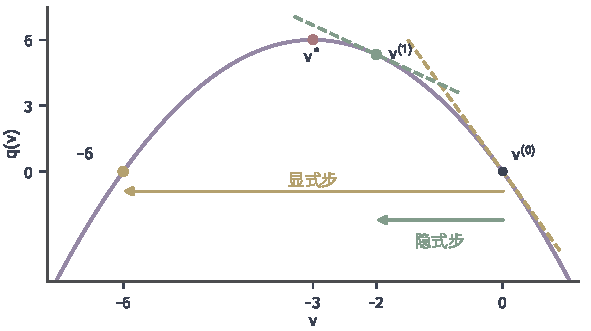
\includegraphics[width=100mm]{figures/05-optimization/06-constrained-optimization/matplotlib/pm-explicit-implicit/figure.pdf}
  \caption{同样的步长$\rho=1.5$下，对偶函数（紫）上的显式步与隐式步。黄色虚线是$\nu^{(0)}=0$处的切线，显式步按它的斜率走到$-6$（黄点）。绿色虚线是$\nu^{(1)}=-2$处的切线，隐式步要求落点切线的斜率与步长一致，得到绿点。红点是最大点$\nu^\star$。}
  \label{fig:pm-explicit-implicit}
\end{BookInlineFigure}

\begin{BookInlineTable}
  \centering
  \begin{tabular}{@{}lll@{}}
    \toprule
     & 对偶上升 & ALM\\
    \midrule
    原始子问题 & $\min\mathcal{L}(\cdot,\bm{\nu})$ & $\min\mathcal{L}_\rho(\cdot,\bm{\nu})$\\
    残差读取点 & 旧乘子（显式） & 新乘子（隐式）\\
    步长限制 & 受$q$的曲率限制 & 任意$\rho>0$（凸问题）\\
    子问题 & 目标可分则可分 & 平方项通常耦合各块\\
    目标线性时 & 子问题可能无解或解不唯一 & 平方项提供曲率\\
    \bottomrule
  \end{tabular}
  \caption{对偶上升与ALM的对照。ALM用更难的子问题换取稳定的乘子更新。}
  \label{tab:pm-dual-vs-alm}
\end{BookInlineTable}

压缩的速度可以显式写出。下面的定理针对最简单的等式约束二次规划，它的结论和图上的行为完全一致。

\begin{theorem}[线性等式二次问题的压缩率]
\label{thm:pm-alm-quadratic-rate}
设$f$是二次函数$\tfrac12\bm{x}^\top\bm{G}\bm{x}-\bm{d}^\top\bm{x}$，$\bm{G}\succ\bm{0}$，$\bm{h}(\bm{x})=\bm{A}\bm{x}-\bm{b}$，$\bm{A}$行满秩，记$\bm{S}=\bm{A}\bm{G}^{-1}\bm{A}^\top$。则精确求解子问题的ALM满足
\begin{equation}
 \bm{\nu}^{(t+1)}-\bm{\nu}^\star=(\bm{I}+\rho\bm{S})^{-1}(\bm{\nu}^{(t)}-\bm{\nu}^\star),
 \label{eq:pm-alm-linear-map}
\end{equation}
于是
\begin{equation}
 \lVert\bm{\nu}^{(t+1)}-\bm{\nu}^\star\rVert_2\leq\frac{1}{1+\rho\,\lambda_{\min}(\bm{S})}\lVert\bm{\nu}^{(t)}-\bm{\nu}^\star\rVert_2 .
 \label{eq:pm-alm-rate}
\end{equation}
\end{theorem}

\begin{proof}
由恒等式~\eqref{eq:pm-al-gradient-identity}，$\bm{x}^{(t+1)}$满足
\[
 \bm{G}\bm{x}^{(t+1)}-\bm{d}+\bm{A}^\top\bm{\nu}^{(t+1)}=\bm{0},
\]
解出
\[
 \bm{x}^{(t+1)}=\bm{G}^{-1}(\bm{d}-\bm{A}^\top\bm{\nu}^{(t+1)}).
\]
代入乘子更新式，得到
\[
 \bm{\nu}^{(t+1)}-\bm{\nu}^{(t)}=\rho\bigl(\bm{A}\bm{G}^{-1}\bm{d}-\bm{S}\bm{\nu}^{(t+1)}-\bm{b}\bigr).
\]
$\bm{\nu}^\star$满足同样形式的方程
\[
 \bm{A}\bm{G}^{-1}\bm{d}-\bm{S}\bm{\nu}^\star-\bm{b}=\bm{0},
\]
两式相减，得到
\[
 \bm{\nu}^{(t+1)}-\bm{\nu}^{(t)}=-\rho\bm{S}(\bm{\nu}^{(t+1)}-\bm{\nu}^\star).
\]
移项得
\[
 (\bm{I}+\rho\bm{S})(\bm{\nu}^{(t+1)}-\bm{\nu}^\star)=\bm{\nu}^{(t)}-\bm{\nu}^\star ,
\]
即式~\eqref{eq:pm-alm-linear-map}。$\bm{S}$对称正定，取范数即得式~\eqref{eq:pm-alm-rate}。
\end{proof}

二元例中$\bm{S}=1+\tfrac13=\tfrac43$，压缩因子是$3/(3+4\rho)$，$\rho=1.5$时为$\tfrac13$。任何$\rho>0$都是压缩的，和对偶上升要求$\alpha<\tfrac32$形成对比。

\paragraph{计算过程}
仍用二元例，并沿用第~\ref{sec:pm-rho-update}小节的外层容差。

\needspace{6\baselineskip}
\paragraph{变量}
\begin{itemize}
 \item $\bm{\nu}^{(t)}\in\mathbb{R}^p$：乘子估计。例中$p=1$。
 \item $\bm{x}^{(t)}\in\mathbb{R}^n$：增广子问题的解。例中$n=2$。
 \item $\rho>0$：罚参数，下一小节讨论它的调整。
\end{itemize}

\paragraph{初始化}
取$\bm{\nu}^{(0)}$和$\rho$。例中$\nu^{(0)}=0$，$\rho=1.5$，外层容差$\varepsilon=0.05$。

\needspace{6\baselineskip}
\paragraph{每轮更新}
\begin{enumerate}
 \item 近似最小化$\mathcal{L}_\rho(\cdot,\bm{\nu}^{(t)})$。例中由式~\eqref{eq:pm-running-al-solution}，$\rho=1.5$时$x_2=(6-\nu)/9$，第一轮
 \[
  \bm{x}^{(1)}=\Bigl(2,\ \frac23\Bigr).
 \]
 \item 计算残差。例中第一轮
 \[
  h(\bm{x}^{(1)})=-\frac43 .
 \]
 \item 由式~\eqref{eq:pm-alm}更新乘子。例中第一轮
 \[
  \nu^{(1)}=0+1.5\times\Bigl(-\frac43\Bigr)=-2 .
 \]
\end{enumerate}
第二轮得到
\[
 \bm{x}^{(2)}=\Bigl(\frac83,\ \frac89\Bigr),\qquad h(\bm{x}^{(2)})=-\frac49,\qquad \nu^{(2)}=-\frac83 .
\]
第三轮得到
\[
 \bm{x}^{(3)}=\Bigl(\frac{26}{9},\ \frac{26}{27}\Bigr),\qquad h(\bm{x}^{(3)})=-\frac{4}{27},\qquad \nu^{(3)}=-\frac{26}{9}.
\]
第四轮得到
\[
 \bm{x}^{(4)}=\Bigl(\frac{80}{27},\ \frac{80}{81}\Bigr),\qquad h(\bm{x}^{(4)})=-\frac{4}{81}\approx-0.049 .
\]

结束条件是$\lvert h\rvert\leq\varepsilon$，例中第四轮满足。最终得到$\bm{x}^{(4)}\approx(2.963,0.988)$，更新后的乘子是$\nu^{(4)}=-\tfrac{80}{27}\approx-2.963$。

第一轮和二次罚$\rho=1.5$的结果相同，因为此时$\nu=0$。此后二次罚换$\rho$，ALM换$\nu$。用相同的梯度法作内层，四轮分别用$21$、$18$、$15$、$12$步，共$66$步，$\rho$一直是$1.5$，条件数一直是$3.1$。

图~\ref{fig:pm-alm-vs-penalty}(a)比较两种方法。按外层轮数看，二次罚（$\rho$每轮乘$10$）下降得更快；但它每一轮都在解一个更病态的问题。ALM每轮只把残差缩小到$\tfrac13$，却始终在解同一个条件数很小的问题。(b)是ALM中$\rho$的取舍：$\rho$越大，外层压缩因子越小，轮数越少，内层条件数越大。

\begin{BookInlineFigure}
  \centering
  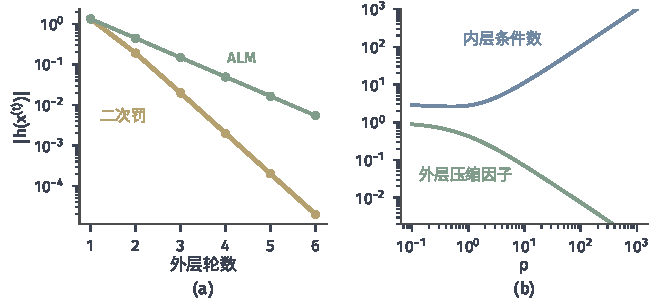
\includegraphics[width=112mm]{figures/05-optimization/06-constrained-optimization/matplotlib/pm-alm-vs-penalty/figure.pdf}
  \caption{二元例上ALM与二次罚的对比。(a)半对数坐标下的约束残差：黄线是二次罚（$\rho$从$1.5$开始每轮乘$10$），绿线是ALM（$\rho=1.5$固定），每轮精确求解。(b)双对数坐标，绿线是ALM的外层压缩因子$3/(3+4\rho)$，蓝线是内层Hessian的条件数。}
  \label{fig:pm-alm-vs-penalty}
\end{BookInlineFigure}

\paragraph{不等式约束}
前面的公式都是等式约束，不等式约束的乘子有符号限制，不能直接照搬。标准的做法是加入非负松弛变量，把$g_i(\bm{x})\leq0$写成$g_i(\bm{x})+s_i=0$，$s_i\geq0$，然后只对这个等式写增广函数。

固定$\bm{x}$，把$s_i$的优化解出来。对第$i$条约束，要在$s_i\geq0$上最小化
\[
 \lambda_i(g_i+s_i)+\frac\rho2(g_i+s_i)^2 .
\]
这是$s_i$的凸二次函数，无约束极小点是$-g_i-\lambda_i/\rho$，投影到非负数后得到
\[
 s_i=\Bigl[-g_i-\frac{\lambda_i}{\rho}\Bigr]_+ .
\]
由此可得$g_i+s_i=\max\{g_i,-\lambda_i/\rho\}$。把它代回去，分$g_i\geq-\lambda_i/\rho$和$g_i<-\lambda_i/\rho$两种情形合并，增广函数为
\begin{equation}
 \mathcal{L}_\rho(\bm{x},\bm{\lambda})=f(\bm{x})+\frac{1}{2\rho}\sum_{i=1}^m\Bigl([\lambda_i+\rho g_i(\bm{x})]_+^2-\lambda_i^2\Bigr).
 \label{eq:pm-al-inequality}
\end{equation}
乘子沿松弛等式更新，$\lambda_i^{+}=\lambda_i+\rho(g_i+s_i)$，整理后是
\begin{equation}
 \lambda_i^{+}=\bigl[\lambda_i+\rho g_i(\bm{x})\bigr]_+ .
 \label{eq:pm-alm-inequality-update}
\end{equation}

这个公式自动带来了对偶可行和互补。$\lambda_i^{+}$是正部，所以非负。若$g_i<-\lambda_i/\rho$，约束有足够余量，$\lambda_i^{+}=0$，该约束暂时不起作用。不动点$\lambda_i^{+}=\lambda_i$等价于$\max\{g_i,-\lambda_i/\rho\}=0$，它恰好是
\begin{equation}
 g_i\leq0,\qquad \lambda_i\geq0,\qquad \lambda_ig_i=0 .
 \label{eq:pm-complementarity}
\end{equation}
图~\ref{fig:pm-alm-ineq}(a)是单条约束的代价：在$g\geq-\lambda/\rho$一侧是二次增长的曲线，另一侧是常数$-\lambda^2/(2\rho)$，两段光滑相接。(b)是乘子更新，折线在$-\lambda/\rho$处把负值截断。

\begin{BookInlineFigure}
  \centering
  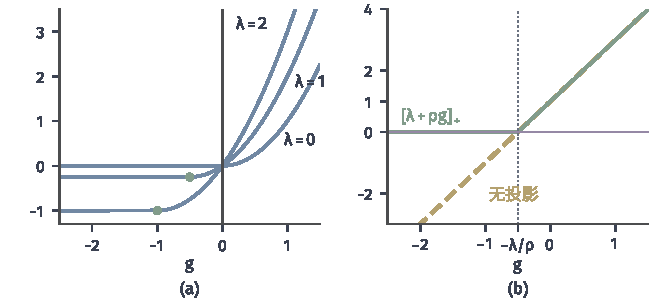
\includegraphics[width=112mm]{figures/05-optimization/06-constrained-optimization/matplotlib/pm-alm-ineq/figure.pdf}
  \caption{不等式约束的增广项，$\rho=2$。(a)蓝线是$([\lambda+\rho g]_+^2-\lambda^2)/(2\rho)$关于$g$的曲线，$\lambda=0,1,2$，绿点是分段点$g=-\lambda/\rho$，深灰竖线是约束边界。(b)$\lambda=1$的乘子更新：绿线是投影形式$[\lambda+\rho g]_+$，黄色虚线是不作投影的直线，紫线是零。}
  \label{fig:pm-alm-ineq}
\end{BookInlineFigure}

用一维例检验。式~\eqref{eq:pm-one-dim}的$g=1-x$，式~\eqref{eq:pm-al-inequality}对$x$的导数是
\[
 1-[\lambda+\rho(1-x)]_+ .
\]
令其为零，得到
\[
 x=1+\frac{\lambda-1}{\rho}.
\]
此时$\lambda+\rho(1-x)=1$，所以由式~\eqref{eq:pm-alm-inequality-update}，不管$\lambda$从哪里开始，一次更新后都有$\lambda^{+}=1=\lambda^\star$。第二轮代入，$x=1$，就是原问题的解。二次罚在同一例上永远差$1/\rho$。

不作投影会出错。考虑$\min x^2$，$x\geq-1$，解$x^\star=0$，约束不活动，$\lambda^\star=0$。写$g=-1-x$，取$\rho=2$，$\lambda^{(0)}=0$。式~\eqref{eq:pm-alm-inequality-update}给出$\lambda^{+}=0$，一步就对。

若把它当作等式，用不带投影的公式，子问题的解是$x=(\lambda-2)/4$，乘子递推是$\lambda^{+}=\tfrac12\lambda-1$。序列$\lambda=0,-1,-1.5,\ldots$趋于$-2$，$x$趋于$-1$。这是把约束当作$x=-1$时的解，既不是原问题的解，乘子的符号也错了。

\subsection{参数与停止条件}
\label{sec:pm-alm-parameters}

ALM的结构已经确定，剩下三件事：什么时候放大$\rho$，子问题解到多准，什么时候算结束。

\paragraph{罚参数}
不必让$\rho$趋于无穷，但也不能太小。$\rho$太小时，一方面非凸问题的子问题可能无下界，另一方面外层压缩很慢。常用的规则是观察约束残差是否下降到位。把等式残差和不等式残差放在同一个向量里：
\begin{equation}
 \bm{c}^{(t)}=\Bigl(\bm{h}(\bm{x}^{(t)}),\ \max\bigl\{\bm{g}(\bm{x}^{(t)}),-\bm{\lambda}^{(t-1)}/\rho^{(t-1)}\bigr\}\Bigr),
 \label{eq:pm-alm-residual-vector}
\end{equation}
其中$\max$按分量取。它把不活动约束的残差也按互补要求记为零。若
\begin{equation}
 \lVert\bm{c}^{(t+1)}\rVert_2>\theta\lVert\bm{c}^{(t)}\rVert_2,
 \label{eq:pm-alm-rho-test}
\end{equation}
说明残差下降不够，令$\rho\leftarrow\beta\rho$，否则保持$\rho$不变。常见取值是$\theta\in[0.25,0.5]$，$\beta\in[2,10]$。

顺序上，先用当前的$\rho$更新乘子，再放大$\rho$。乘子本身是一个不依赖$\rho$的量，放大$\rho$不需要换算它。

例如二元例若从$\rho=0.15$开始，压缩因子是$3/3.6\approx0.83$。第一轮和第二轮的结果为
\[
 h(\bm{x}^{(1)})=-\frac{10}{3},\qquad h(\bm{x}^{(2)})=-\frac{25}{9}.
\]
第二轮的残差比是$0.83$，大于$\theta=0.5$，所以把$\rho$放大到$1.5$，此后压缩因子变成$\tfrac13$。

\paragraph{内层精度}
恒等式~\eqref{eq:pm-al-gradient-identity}给出了一个便利之处：增广函数的内层梯度$\lVert\nabla_{\bm{x}}\mathcal{L}_\rho(\bm{x},\bm{\nu}^{(t)})\rVert_2$，正是更新后的乘子下Lagrange驻定残差。所以内层容差就是外层驻定精度，不用另算。

外层初期乘子还不准，把子问题解得太细是浪费。常用的安排是让内层容差$\omega^{(t)}$随外层逐步收紧，最终降到所需的驻定精度。对凸问题，邻近点法的分析要求内层误差可和，$\sum_t\epsilon^{(t)}<\infty$；实现上也常用与约束残差挂钩的相对准则。

\paragraph{三类残差}
结束时要分别检查三项，任何一项不合格都不算解好：
\begin{equation}
 \begin{aligned}
 \text{原始可行：}\quad&\lVert\bm{h}(\bm{x})\rVert_2,\ \ \lVert[\bm{g}(\bm{x})]_+\rVert_2\leq\varepsilon_{\mathrm{p}},\\
 \text{Lagrange驻定：}\quad&\lVert\nabla_{\bm{x}}\mathcal{L}(\bm{x},\bm{\lambda}^{+},\bm{\nu}^{+})\rVert_2\leq\varepsilon_{\mathrm{d}},\\
 \text{互补：}\quad&\lVert\min\{-\bm{g}(\bm{x}),\bm{\lambda}^{+}\}\rVert_2\leq\varepsilon_{\mathrm{c}}.
 \end{aligned}
 \label{eq:pm-alm-stopping}
\end{equation}
其中$\min$按分量取，它为零当且仅当式~\eqref{eq:pm-complementarity}成立。式中的第二项对应恒等式~\eqref{eq:pm-al-gradient-identity}，第一项不会因为内层解得准而自动变小，这一点和二次罚相同。

\paragraph{能保证什么}
ALM的保证分成三个层次，所需条件依次不同。先证明凸问题的情形，证明本身也说明了$\rho$为什么影响外层。

\begin{theorem}[凸问题的固定参数收敛]
\label{thm:pm-alm-convex}
设$f$是适当、闭的凸函数，$\bm{h}(\bm{x})=\bm{A}\bm{x}-\bm{b}$，存在最优解和最优乘子$\bm{\nu}^\star$，且强对偶成立。设$\rho>0$固定，各子问题的全局最小点存在且精确求解，$\bm{s}^{(t)}=\bm{h}(\bm{x}^{(t)})$。则
\begin{equation}
 \sum_{t\geq1}\rho^2\lVert\bm{s}^{(t)}\rVert_2^2\leq\lVert\bm{\nu}^{(0)}-\bm{\nu}^\star\rVert_2^2,
 \label{eq:pm-alm-summable}
\end{equation}
并且$\bm{h}(\bm{x}^{(t)})\to\bm{0}$，$q(\bm{\nu}^{(t)})\to d^\star$，$f(\bm{x}^{(t)})\to f^\star$。
\end{theorem}

\begin{proof}
记$\bm{\nu}=\bm{\nu}^{(t-1)}$，$\bm{\nu}^{+}=\bm{\nu}^{(t)}$，$\bm{s}^{+}=\bm{s}^{(t)}$。由定理~\ref{thm:pm-alm-proximal}，$\bm{s}^{+}$是$q$在$\bm{\nu}^{+}$处的超梯度。在式~\eqref{eq:pm-supergradient}中取比较点$\bm{\nu}^\star$，得到
\[
 q(\bm{\nu}^\star)\leq q(\bm{\nu}^{+})+\langle\bm{s}^{+},\bm{\nu}^\star-\bm{\nu}^{+}\rangle .
\]
$\bm{\nu}^\star$是$q$的最大点，所以$q(\bm{\nu}^{+})\leq q(\bm{\nu}^\star)$，上式给出
\[
 \langle\bm{s}^{+},\bm{\nu}^{+}-\bm{\nu}^\star\rangle\leq0 .
\]
现在把$\bm{\nu}=\bm{\nu}^{+}-\rho\bm{s}^{+}$代入$\lVert\bm{\nu}-\bm{\nu}^\star\rVert_2^2$并展开：
\[
 \lVert\bm{\nu}-\bm{\nu}^\star\rVert_2^2=\lVert\bm{\nu}^{+}-\bm{\nu}^\star\rVert_2^2-2\rho\langle\bm{s}^{+},\bm{\nu}^{+}-\bm{\nu}^\star\rangle+\rho^2\lVert\bm{s}^{+}\rVert_2^2 .
\]
中间项非负，舍去后得到
\[
 \lVert\bm{\nu}^{+}-\bm{\nu}^\star\rVert_2^2+\rho^2\lVert\bm{s}^{+}\rVert_2^2\leq\lVert\bm{\nu}-\bm{\nu}^\star\rVert_2^2 .
\]
对$t$求和裂项，即得式~\eqref{eq:pm-alm-summable}，于是$\bm{s}^{(t)}\to\bm{0}$，且$\bm{\nu}^{(t)}$有界。

再由第一个不等式，
\[
 0\leq d^\star-q(\bm{\nu}^{+})\leq\langle\bm{s}^{+},\bm{\nu}^\star-\bm{\nu}^{+}\rangle\leq\lVert\bm{s}^{+}\rVert_2\lVert\bm{\nu}^\star-\bm{\nu}^{+}\rVert_2\to0 .
\]
最后，由定理~\ref{thm:pm-alm-proximal}，$\bm{x}^{(t)}$是$\mathcal{L}(\cdot,\bm{\nu}^{(t)})$的全局最小点，所以
\[
 f(\bm{x}^{(t)})=q(\bm{\nu}^{(t)})-\langle\bm{\nu}^{(t)},\bm{s}^{(t)}\rangle ,
\]
右边趋于$d^\star=f^\star$。
\end{proof}

式~\eqref{eq:pm-alm-summable}中的$\rho^2$说明，$\rho$越大，残差平方的总和越小，外层越快。定理既不要求$\rho$放大，也不要求$f$可微，并且$\bm{x}^{(t)}$本身不一定收敛，$f$不强凸时子问题的解可以不唯一。

非凸问题只有局部结论。设$(\bm{x}^\star,\bm{\nu}^\star)$满足KKT条件，LICQ和二阶充分条件成立。那么存在$\bar\rho$，当$\rho\geq\bar\rho$时，从足够接近$\bm{\nu}^\star$的乘子出发，取$\mathcal{L}_\rho$在$\bm{x}^\star$附近的局部最小点，乘子序列线性收敛到$\bm{\nu}^\star$，压缩因子约为$O(1/\rho)$。这一结论的证明需要对驻定方程应用隐函数定理，篇幅较长，读者可查阅Nocedal和Wright的著作\scite{math-nocedal2006numerical}，它的机制和式~\eqref{eq:pm-alm-rate}相同。

全局层次的结果最弱。若每个子问题只解到近似驻点，乘子保持有界（常把估计截断在一个大盒子里），可以证明聚点要么是约束违规量的驻点，要么在相应约束资格下是KKT点；和定理~\ref{thm:pm-quadratic-approximate}的结论是同一类型。只有每个子问题都取全局最小点，才能得到全局最优的结论，非凸问题通常做不到。下表把三个层次放在一起。

\begin{BookInlineTable}
  \centering
  \small
  \begin{tabular}{@{}lll@{}}
    \toprule
    情形 & 主要条件 & 结论\\
    \midrule
    凸，固定$\rho$ & 强对偶，子问题精确 & 残差趋零，目标值收敛\\
    非凸，局部 & LICQ，二阶充分，$\rho\geq\bar\rho$ & 乘子局部线性收敛\\
    非凸，全局策略 & 近似驻点，乘子有界 & 聚点为不可行驻点或KKT点\\
    \bottomrule
  \end{tabular}
  \caption{ALM的三层保证。下面一行不能推出上面两行的结论。}
  \label{tab:pm-alm-guarantees}
\end{BookInlineTable}

\section{交替方向乘子法（ADMM）}
\label{sec:pm-admm}

ALM的子问题比对偶上升的子问题难的地方，在于平方项把各块耦合了。于是要问：当目标由两块组成，能否既保留乘子带来的稳定性，又把两块分开计算？本节的问题形式是
\begin{equation}
 \min_{\bm{x},\bm{z}}\ f(\bm{x})+g(\bm{z})\qquad\text{s.t.}\qquad\bm{A}\bm{x}+\bm{B}\bm{z}=\bm{c},
 \label{eq:pm-admm-problem}
\end{equation}
其中$\bm{x}\in\mathbb{R}^n$，$\bm{z}\in\mathbb{R}^l$，$\bm{A}\in\mathbb{R}^{p\times n}$，$\bm{B}\in\mathbb{R}^{p\times l}$，$\bm{c}\in\mathbb{R}^p$。这里的$g$是第二块目标，不是不等式约束。对应的增广Lagrange函数是
\begin{equation}
 \mathcal{L}_\rho(\bm{x},\bm{z},\bm{\nu})=f(\bm{x})+g(\bm{z})+\langle\bm{\nu},\bm{A}\bm{x}+\bm{B}\bm{z}-\bm{c}\rangle+\frac\rho2\lVert\bm{A}\bm{x}+\bm{B}\bm{z}-\bm{c}\rVert_2^2 .
 \label{eq:pm-admm-al}
\end{equation}

\paragraph{平方项破坏了可分性}
对偶分解能并行，靠的是Lagrange函数按块可分。增广函数的平方项里有交叉项$\rho\langle\bm{A}\bm{x},\bm{B}\bm{z}\rangle$，可分性被破坏。ALM只能把$(\bm{x},\bm{z})$联合起来最小化，即使$f$和$g$各自都很简单。

\term{交替方向乘子法}（alternating direction method of multipliers，ADMM）的想法是：不把子问题解到最优，只把$\bm{x}$和$\bm{z}$各自更新一次，然后立即更新乘子。

这个想法要付代价。用二元例说明，把它看成$f(x)=\tfrac12x^2$，$g(z)=\tfrac32z^2$，$x+z=4$，$\rho=1.5$，$\nu=0$。联合最小化$\mathcal{L}_\rho$得到式~\eqref{eq:pm-running-al-solution}，即$(x,z)=(2,\tfrac23)$。

从$(0,0)$开始交替一次：先固定$z=0$，对$x$最小化，$x=\tfrac{\rho\cdot4}{1+\rho}=2.4$；再固定$x=2.4$，对$z$最小化，$z=\tfrac{\rho(4-2.4)}{3+\rho}=\tfrac{8}{15}$。结果是$(2.4,\tfrac{8}{15})$，与联合解$(2,\tfrac23)$不同。

图~\ref{fig:pm-admm-sweep}(a)画出了这两步：黄色折线先水平走，再竖直走，两步都只顾自己的方向，没有到达碗底。一次交替扫过两块，不等于把子问题解到最优，所以不能把ALM的结论直接搬过来。(b)是多轮的路径，ADMM走的是折线，ALM走的是直线，两者最后都到达红点。

\begin{BookInlineFigure}
  \centering
  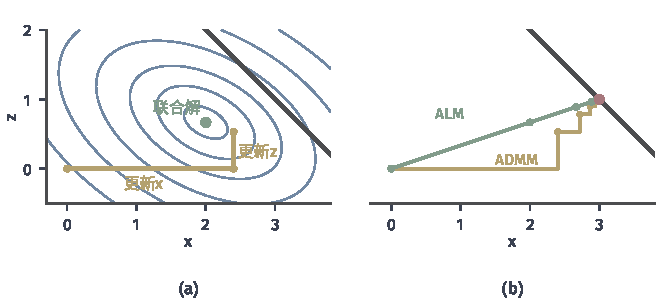
\includegraphics[width=112mm]{figures/05-optimization/06-constrained-optimization/matplotlib/pm-admm-sweep/figure.pdf}
  \caption{二元例上ADMM的两块交替更新，$\rho=1.5$。深灰直线是约束。(a)蓝线是$\nu=0$时增广函数的等高线，绿点是联合最小点$(2,\tfrac23)$，黄色折线是从原点出发的一次交替，停在$(2.4,\tfrac{8}{15})$。(b)绿线是ALM每轮的联合解，黄线是ADMM的折线路径，红点是解$(3,1)$。}
  \label{fig:pm-admm-sweep}
\end{BookInlineFigure}

\subsection{两块交替更新}
\label{sec:pm-admm-update}

\paragraph{主要思想}
每轮按固定的顺序做三步，后一步使用前一步刚得到的结果，如图~\ref{fig:pm-admm-flow}所示：
\begin{equation}
 \begin{aligned}
 \bm{x}^{(t+1)}&\in\argmin_{\bm{x}}\mathcal{L}_\rho(\bm{x},\bm{z}^{(t)},\bm{\nu}^{(t)}),\\
 \bm{z}^{(t+1)}&\in\argmin_{\bm{z}}\mathcal{L}_\rho(\bm{x}^{(t+1)},\bm{z},\bm{\nu}^{(t)}),\\
 \bm{\nu}^{(t+1)}&=\bm{\nu}^{(t)}+\rho\bigl(\bm{A}\bm{x}^{(t+1)}+\bm{B}\bm{z}^{(t+1)}-\bm{c}\bigr).
 \end{aligned}
 \label{eq:pm-admm}
\end{equation}

\begin{BookInlineFigure}
  \centering
  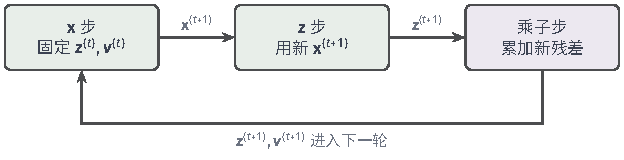
\includegraphics[width=105mm]{figures/05-optimization/06-constrained-optimization/tikz/pm-admm-flow/figure.pdf}
  \caption{ADMM一轮的三步。绿框是两个原始变量的最小化，后一块使用前一块的新值；紫框按新残差累加乘子。与ALM的区别在于$\bm{x}$和$\bm{z}$不联合求解。}
  \label{fig:pm-admm-flow}
\end{BookInlineFigure}

这和第~\ref{chap:block-optimization}章的分块最小化很像：在固定的目标上逐块求最小。两者的区别在于这里有线性耦合约束，单纯的分块下降可能卡在不是解的点上，ADMM靠乘子一步把约束信息累加进下一轮。

\paragraph{缩放乘子}
把乘子除以$\rho$，公式会简短很多。记残差$\bm{r}=\bm{A}\bm{x}+\bm{B}\bm{z}-\bm{c}$，配方得
\[
 \langle\bm{\nu},\bm{r}\rangle+\frac\rho2\lVert\bm{r}\rVert_2^2=\frac\rho2\lVert\bm{r}+\bm{u}\rVert_2^2-\frac\rho2\lVert\bm{u}\rVert_2^2,\qquad\bm{u}=\frac{\bm{\nu}}{\rho}.
\]

$\bm{u}$称为\term{缩放乘子}（scaled dual variable）。式~\eqref{eq:pm-admm}写成缩放形式是
\begin{equation}
 \begin{aligned}
 \bm{x}^{(t+1)}&\in\argmin_{\bm{x}}\ f(\bm{x})+\frac\rho2\lVert\bm{A}\bm{x}+\bm{B}\bm{z}^{(t)}-\bm{c}+\bm{u}^{(t)}\rVert_2^2,\\
 \bm{z}^{(t+1)}&\in\argmin_{\bm{z}}\ g(\bm{z})+\frac\rho2\lVert\bm{A}\bm{x}^{(t+1)}+\bm{B}\bm{z}-\bm{c}+\bm{u}^{(t)}\rVert_2^2,\\
 \bm{u}^{(t+1)}&=\bm{u}^{(t)}+\bm{A}\bm{x}^{(t+1)}+\bm{B}\bm{z}^{(t+1)}-\bm{c}.
 \end{aligned}
 \label{eq:pm-admm-scaled}
\end{equation}
两种写法完全等价。缩放乘子就是残差的累加和，这是它最直观的含义：$\bm{u}^{(t)}$记录到目前为止累计的残差。

\paragraph{套索问题的拆分}
ADMM的用处是把一个有结构的问题拆成两个容易的问题。第~\ref{chap:nonsmooth-composite-optimization}章的套索问题是
\begin{equation}
 \min_{\bm{x}}\ \frac12\lVert\bm{D}\bm{x}-\bm{y}\rVert_2^2+\gamma\lVert\bm{x}\rVert_1 ,
 \label{eq:pm-lasso}
\end{equation}
其中$\bm{D}\in\mathbb{R}^{N\times n}$，$\gamma>0$。把变量复制一份，让$f$负责最小二乘项$\tfrac12\lVert\bm{D}\bm{x}-\bm{y}\rVert_2^2$，$g$负责$\gamma\lVert\bm{z}\rVert_1$，并加上约束$\bm{x}-\bm{z}=\bm{0}$。这对应$\bm{A}=\bm{I}$，$\bm{B}=-\bm{I}$，$\bm{c}=\bm{0}$。

把$f$代入式~\eqref{eq:pm-admm-scaled}的第一行，这是一个二次子问题，解为
\begin{equation}
 \bm{x}^{(t+1)}=(\bm{D}^\top\bm{D}+\rho\bm{I})^{-1}\bigl(\bm{D}^\top\bm{y}+\rho(\bm{z}^{(t)}-\bm{u}^{(t)})\bigr).
 \label{eq:pm-lasso-x}
\end{equation}
第二行是$\gamma\lVert\bm{z}\rVert_1$加上一个以$\bm{x}^{(t+1)}+\bm{u}^{(t)}$为中心的二次项，按坐标可分，由软阈值给出：
\begin{equation}
 \bm{z}^{(t+1)}=S_{\gamma/\rho}\bigl(\bm{x}^{(t+1)}+\bm{u}^{(t)}\bigr),\qquad
 S_\tau(a)=\operatorname{sign}(a)\max\{\lvert a\rvert-\tau,0\}.
 \label{eq:pm-lasso-z}
\end{equation}
第三行是缩放乘子的累加：
\begin{equation}
 \bm{u}^{(t+1)}=\bm{u}^{(t)}+\bm{x}^{(t+1)}-\bm{z}^{(t+1)}.
 \label{eq:pm-lasso-u}
\end{equation}
二次子问题只含$f$，软阈值只含$g$，这样两部分结构都得到了利用。

\paragraph{计算过程}
用第~\ref{chap:nonsmooth-composite-optimization}章的小例子演示，数据是
\[
 \bm{D}=\begin{pmatrix}1&1\\1&0\\0&1\end{pmatrix},\qquad
 \bm{y}=\begin{pmatrix}3\\2\\-1\end{pmatrix},\qquad
 \gamma=1 .
\]
这个问题的解是$\bm{x}^\star=(2,0)$，由它算出乘子
\[
 \bm{\nu}^\star=\bm{D}^\top(\bm{y}-\bm{D}\bm{x}^\star)=(1,0).
\]

\needspace{6\baselineskip}
\paragraph{变量}
\begin{itemize}
 \item $\bm{x}^{(t)},\bm{z}^{(t)}\in\mathbb{R}^n$：两块原始变量。例中$n=2$。
 \item $\bm{u}^{(t)}\in\mathbb{R}^n$：缩放乘子。
 \item $(\bm{D}^\top\bm{D}+\rho\bm{I})^{-1}$：只需计算一次的矩阵分解。
\end{itemize}

\paragraph{初始化}
取$\bm{z}^{(0)}$、$\bm{u}^{(0)}$和$\rho$。例中$\bm{z}^{(0)}=\bm{u}^{(0)}=\bm{0}$，$\rho=1$，并预先算出
\[
 \bm{D}^\top\bm{y}=\begin{pmatrix}5\\2\end{pmatrix},\qquad
 (\bm{D}^\top\bm{D}+\bm{I})^{-1}=\frac18\begin{pmatrix}3&-1\\-1&3\end{pmatrix}.
\]

\needspace{6\baselineskip}
\paragraph{每轮更新}
\begin{enumerate}
 \item 由式~\eqref{eq:pm-lasso-x}算$\bm{x}^{(t+1)}$。例中第一轮
 \[
  \bm{x}^{(1)}=\frac18\begin{pmatrix}3&-1\\-1&3\end{pmatrix}\begin{pmatrix}5\\2\end{pmatrix}=\begin{pmatrix}1.625\\0.125\end{pmatrix}.
 \]
 \item 由式~\eqref{eq:pm-lasso-z}算$\bm{z}^{(t+1)}$，阈值是$\gamma/\rho=1$。例中第一轮
 \[
  \bm{z}^{(1)}=S_1(1.625,\ 0.125)=(0.625,\ 0).
 \]
 \item 由式~\eqref{eq:pm-lasso-u}累加残差。例中第一轮
 \[
  \bm{u}^{(1)}=(1,\ 0.125).
 \]
\end{enumerate}
第二轮中，式~\eqref{eq:pm-lasso-x}的右端向量是$(4.625,1.875)$，得到
\[
 \bm{x}^{(2)}=(1.5,\ 0.125),\qquad \bm{z}^{(2)}=(1.5,\ 0),\qquad \bm{u}^{(2)}=(1,\ 0.25).
\]
第三轮中，右端向量是$(5.5,1.75)$，得到
\[
 \bm{x}^{(3)}=(1.84375,\,-0.03125),\quad \bm{z}^{(3)}=(1.84375,\,0),\quad \bm{u}^{(3)}=(1,\,0.21875).
\]

结束条件由下一小节的残差给出。例中$\bm{z}^{(t)}$从第一轮起就有第二个分量恰好为零，这是软阈值带来的。而$\bm{x}^{(t)}$的第二个分量不为零，只有极限才为零。继续迭代，$24$轮后两种残差都小于$10^{-6}$，最终得到$\bm{z}\approx(2,0)$，$\bm{u}\approx(1,0)$，与上面的$\bm{x}^\star$和$\bm{\nu}^\star$一致。

\subsection{原始与对偶残差}
\label{sec:pm-admm-residuals}

\paragraph{两类残差的来历}
判断ADMM是否收敛，要回到KKT条件。问题~\eqref{eq:pm-admm-problem}的KKT条件有三条：
\begin{equation}
 \bm{A}\bm{x}^\star+\bm{B}\bm{z}^\star=\bm{c},\qquad
 \bm{0}\in\partial f(\bm{x}^\star)+\bm{A}^\top\bm{\nu}^\star,\qquad
 \bm{0}\in\partial g(\bm{z}^\star)+\bm{B}^\top\bm{\nu}^\star .
 \label{eq:pm-admm-kkt}
\end{equation}
第一条对应\term{原始残差}（primal residual）：
\begin{equation}
 \bm{r}^{(t+1)}=\bm{A}\bm{x}^{(t+1)}+\bm{B}\bm{z}^{(t+1)}-\bm{c}.
 \label{eq:pm-admm-primal-residual}
\end{equation}
它度量约束违规。

后两条要看子问题的最优性条件。$\bm{z}^{(t+1)}$最小化$\mathcal{L}_\rho(\bm{x}^{(t+1)},\cdot,\bm{\nu}^{(t)})$，所以
\[
 \bm{0}\in\partial g(\bm{z}^{(t+1)})+\bm{B}^\top\bm{\nu}^{(t)}+\rho\bm{B}^\top\bm{r}^{(t+1)}=\partial g(\bm{z}^{(t+1)})+\bm{B}^\top\bm{\nu}^{(t+1)}.
\]
第三条KKT条件每一轮都自动成立。这也说明了乘子步长取成$\rho$的原因，和式~\eqref{eq:pm-al-gradient-identity}是同一个道理。

$\bm{x}^{(t+1)}$的最优性条件里，用的是旧的$\bm{z}^{(t)}$：
\[
 \bm{0}\in\partial f(\bm{x}^{(t+1)})+\bm{A}^\top\bm{\nu}^{(t)}+\rho\bm{A}^\top\bigl(\bm{A}\bm{x}^{(t+1)}+\bm{B}\bm{z}^{(t)}-\bm{c}\bigr).
\]
用乘子更新式把$\bm{\nu}^{(t)}$换成$\bm{\nu}^{(t+1)}$，整理得到
\begin{equation}
 \rho\bm{A}^\top\bm{B}(\bm{z}^{(t+1)}-\bm{z}^{(t)})\in\partial f(\bm{x}^{(t+1)})+\bm{A}^\top\bm{\nu}^{(t+1)}.
 \label{eq:pm-admm-x-optimality}
\end{equation}
左边的向量就是第二条KKT条件还差的部分，这是\term{对偶残差}（dual residual）：
\begin{equation}
 \bm{s}^{(t+1)}=\rho\bm{A}^\top\bm{B}(\bm{z}^{(t+1)}-\bm{z}^{(t)}).
 \label{eq:pm-admm-dual-residual}
\end{equation}
对偶残差的来源，是$\bm{x}$更新时用了$\bm{z}$的旧值。如果$\bm{x},\bm{z}$是联合求解的，它就恒为零，这正是ALM没有这一项的原因。

例中$\bm{A}=\bm{I}$，$\bm{B}=-\bm{I}$，所以
\[
 \lVert\bm{r}^{(t)}\rVert_2=\lVert\bm{x}^{(t)}-\bm{z}^{(t)}\rVert_2,\qquad
 \lVert\bm{s}^{(t)}\rVert_2=\rho\lVert\bm{z}^{(t)}-\bm{z}^{(t-1)}\rVert_2 .
\]
上面三轮的数值是
\[
 \lVert\bm{r}^{(1)}\rVert_2\approx1.008,\qquad\lVert\bm{r}^{(2)}\rVert_2=0.125,\qquad\lVert\bm{r}^{(3)}\rVert_2\approx0.031,
\]
\[
 \lVert\bm{s}^{(1)}\rVert_2=0.625,\qquad\lVert\bm{s}^{(2)}\rVert_2=0.875,\qquad\lVert\bm{s}^{(3)}\rVert_2\approx0.344 .
\]
可见两个残差并不同步，第二轮原始残差下降，对偶残差反而上升。只看其中一个会误判。图~\ref{fig:pm-admm-lasso}(a)是完整的残差曲线。

\paragraph{停止准则}
两个残差都小才算结束。残差的量级依赖数据的量级，所以常用绝对容差$\varepsilon_{\mathrm{abs}}$和相对容差$\varepsilon_{\mathrm{rel}}$的组合：
\begin{equation}
 \begin{aligned}
 \lVert\bm{r}^{(t)}\rVert_2&\leq\sqrt{p}\,\varepsilon_{\mathrm{abs}}+\varepsilon_{\mathrm{rel}}\max\bigl\{\lVert\bm{A}\bm{x}^{(t)}\rVert_2,\lVert\bm{B}\bm{z}^{(t)}\rVert_2,\lVert\bm{c}\rVert_2\bigr\},\\
 \lVert\bm{s}^{(t)}\rVert_2&\leq\sqrt{n}\,\varepsilon_{\mathrm{abs}}+\varepsilon_{\mathrm{rel}}\lVert\bm{A}^\top\bm{\nu}^{(t)}\rVert_2 .
 \end{aligned}
 \label{eq:pm-admm-stopping}
\end{equation}
绝对容差防止目标为零附近时相对准则失效，$\sqrt{p}$和$\sqrt{n}$让绝对容差按每个分量计。

\paragraph{罚参数的影响与调整}
$\rho$在两个残差之间做权衡。$\rho$大，约束被更用力地压住，原始残差小；可$\bm{s}$正比于$\rho$，对偶残差变大。$\rho$小时情况相反。图~\ref{fig:pm-admm-lasso}(b)是轮数随$\rho$变化的曲线，有一个相当宽的最佳区间，两端都很慢。

一种常见的启发式规则是让两个残差保持同一量级：
\begin{equation}
 \rho^{(t+1)}=
 \begin{cases}
 2\rho^{(t)}, & \lVert\bm{r}^{(t)}\rVert_2>10\lVert\bm{s}^{(t)}\rVert_2,\\
 \rho^{(t)}/2, & \lVert\bm{s}^{(t)}\rVert_2>10\lVert\bm{r}^{(t)}\rVert_2,\\
 \rho^{(t)}, & \text{其他}.
 \end{cases}
 \label{eq:pm-admm-rho}
\end{equation}
这称为\term{残差平衡}（residual balancing）。改变$\rho$时要特别注意缩放乘子。未缩放的$\bm{\nu}$不变，所以$\bm{u}=\bm{\nu}/\rho$必须同步换算：
\begin{equation}
 \bm{u}\leftarrow\frac{\rho^{(t)}}{\rho^{(t+1)}}\bm{u}.
 \label{eq:pm-admm-rescale}
\end{equation}
忘记换算，相当于悄悄改变了乘子，迭代会被打乱。此外，$\rho$变化后需要重新分解矩阵，下面的收敛定理也只对固定的$\rho$成立，实际中常在迭代若干轮后固定$\rho$。

\begin{BookInlineFigure}
  \centering
  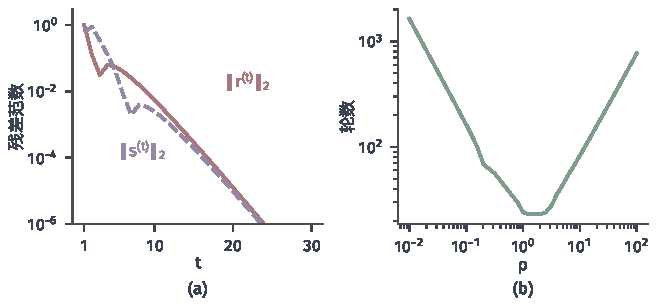
\includegraphics[width=112mm]{figures/05-optimization/06-constrained-optimization/matplotlib/pm-admm-lasso/figure.pdf}
  \caption{小例子上的ADMM。(a)半对数坐标，$\rho=1$，红线是原始残差，紫色虚线是对偶残差。(b)双对数坐标，两个残差都小于$10^{-6}$所需的轮数随$\rho$的变化。两端都慢，中间有一段较宽的平坦区域。}
  \label{fig:pm-admm-lasso}
\end{BookInlineFigure}

\subsection{收敛与实现}
\label{sec:pm-admm-convergence}

\paragraph{收敛定理}
ADMM的步子不是ALM的精确子问题，上一节的定理不能直接用，需要一个专门的证明。证明的想法是构造一个Lyapunov函数，它把乘子误差和$\bm{z}$的误差放在一起，每一轮都下降。

\begin{theorem}[两块ADMM的收敛]
\label{thm:pm-admm-convergence}
设$f,g$是适当、闭的凸函数，固定$\rho>0$，式~\eqref{eq:pm-admm}的两个子问题的最小点存在并精确求解。设$\mathcal{L}_0$有鞍点$(\bm{x}^\star,\bm{z}^\star,\bm{\nu}^\star)$，记$p^\star=f(\bm{x}^\star)+g(\bm{z}^\star)$，$p^{(t)}=f(\bm{x}^{(t)})+g(\bm{z}^{(t)})$，并记
\begin{equation}
 V^{(t)}=\frac1\rho\lVert\bm{\nu}^{(t)}-\bm{\nu}^\star\rVert_2^2+\rho\lVert\bm{B}(\bm{z}^{(t)}-\bm{z}^\star)\rVert_2^2 .
 \label{eq:pm-admm-lyapunov}
\end{equation}
则$t\geq1$时
\begin{equation}
 V^{(t+1)}\leq V^{(t)}-\rho\lVert\bm{r}^{(t+1)}\rVert_2^2-\rho\lVert\bm{B}(\bm{z}^{(t+1)}-\bm{z}^{(t)})\rVert_2^2 ,
 \label{eq:pm-admm-descent}
\end{equation}
并且$\bm{r}^{(t)}\to\bm{0}$，$\bm{s}^{(t)}\to\bm{0}$，$p^{(t)}\to p^\star$。若$\bm{A},\bm{B}$还列满秩，则$\bm{x}^{(t)},\bm{z}^{(t)},\bm{\nu}^{(t)}$都收敛，其极限构成一个鞍点。
\end{theorem}

\begin{proof}
记$\bm{r}=\bm{r}^{(t+1)}$，$\bm{w}=\bm{B}(\bm{z}^{(t+1)}-\bm{z}^{(t)})$。证明分四步。

第一步，用鞍点给出一侧不等式。鞍点满足
\[
 \mathcal{L}_0(\bm{x}^\star,\bm{z}^\star,\bm{\nu}^\star)\leq\mathcal{L}_0(\bm{x}^{(t+1)},\bm{z}^{(t+1)},\bm{\nu}^\star),
\]
再用$\bm{A}\bm{x}^\star+\bm{B}\bm{z}^\star=\bm{c}$，于是
\begin{equation}
 p^\star-p^{(t+1)}\leq\langle\bm{\nu}^\star,\bm{r}\rangle .
 \label{eq:pm-admm-proof-a}
\end{equation}

第二步，用子问题的最优性给出另一侧不等式。上一小节已经推导，$\bm{x}^{(t+1)}$最小化凸函数$f(\bm{x})+\langle\bm{\nu}^{(t+1)}-\rho\bm{w},\bm{A}\bm{x}\rangle$，$\bm{z}^{(t+1)}$最小化凸函数$g(\bm{z})+\langle\bm{\nu}^{(t+1)},\bm{B}\bm{z}\rangle$。分别在$\bm{x}^\star$、$\bm{z}^\star$处比较，得到
\[
 f(\bm{x}^{(t+1)})+\langle\bm{\nu}^{(t+1)}-\rho\bm{w},\bm{A}\bm{x}^{(t+1)}\rangle\leq f(\bm{x}^\star)+\langle\bm{\nu}^{(t+1)}-\rho\bm{w},\bm{A}\bm{x}^\star\rangle,
\]
\[
 g(\bm{z}^{(t+1)})+\langle\bm{\nu}^{(t+1)},\bm{B}\bm{z}^{(t+1)}\rangle\leq g(\bm{z}^\star)+\langle\bm{\nu}^{(t+1)},\bm{B}\bm{z}^\star\rangle .
\]
两式相加。由$\bm{A}\bm{x}^\star+\bm{B}\bm{z}^\star=\bm{c}$，有
\[
 \bm{A}(\bm{x}^{(t+1)}-\bm{x}^\star)+\bm{B}(\bm{z}^{(t+1)}-\bm{z}^\star)=\bm{r},
\]
所以含$\bm{\nu}^{(t+1)}$的项合并成$\langle\bm{\nu}^{(t+1)},\bm{r}\rangle$。再把$\bm{A}(\bm{x}^{(t+1)}-\bm{x}^\star)$换成$\bm{r}-\bm{B}(\bm{z}^{(t+1)}-\bm{z}^\star)$，得到
\begin{equation}
 p^{(t+1)}-p^\star\leq-\langle\bm{\nu}^{(t+1)},\bm{r}\rangle+\rho\langle\bm{w},\bm{r}-\bm{B}(\bm{z}^{(t+1)}-\bm{z}^\star)\rangle .
 \label{eq:pm-admm-proof-b}
\end{equation}

第三步，推导下降不等式。式~\eqref{eq:pm-admm-proof-a}与式~\eqref{eq:pm-admm-proof-b}相加，左边为零，两边乘$2$并移项，得到
\[
 2\langle\bm{\nu}^{(t+1)}-\bm{\nu}^\star,\bm{r}\rangle-2\rho\langle\bm{w},\bm{r}\rangle+2\rho\langle\bm{w},\bm{B}(\bm{z}^{(t+1)}-\bm{z}^\star)\rangle\leq0 .
\]

第一项用$\bm{\nu}^{(t+1)}=\bm{\nu}^{(t)}+\rho\bm{r}$改写，按乘子距离的平方差展开：
\[
 2\langle\bm{\nu}^{(t+1)}-\bm{\nu}^\star,\bm{r}\rangle
 =\frac1\rho\Bigl(\lVert\bm{\nu}^{(t+1)}-\bm{\nu}^\star\rVert_2^2-\lVert\bm{\nu}^{(t)}-\bm{\nu}^\star\rVert_2^2\Bigr)+\rho\lVert\bm{r}\rVert_2^2 .
\]
第三项要用下面的恒等式：
\[
 2\langle\bm{a}-\bm{b},\bm{a}\rangle=\lVert\bm{a}\rVert_2^2-\lVert\bm{b}\rVert_2^2+\lVert\bm{a}-\bm{b}\rVert_2^2 .
\]
取$\bm{a}=\bm{B}(\bm{z}^{(t+1)}-\bm{z}^\star)$，$\bm{b}=\bm{B}(\bm{z}^{(t)}-\bm{z}^\star)$，此时$\bm{a}-\bm{b}=\bm{w}$，于是
\[
 2\rho\langle\bm{w},\bm{a}\rangle=\rho\lVert\bm{a}\rVert_2^2-\rho\lVert\bm{b}\rVert_2^2+\rho\lVert\bm{w}\rVert_2^2 .
\]
把这两式代回，合并成
\[
 V^{(t+1)}-V^{(t)}+\rho\lVert\bm{r}\rVert_2^2+\rho\lVert\bm{w}\rVert_2^2-2\rho\langle\bm{w},\bm{r}\rangle\leq0 .
\]

只差$\langle\bm{w},\bm{r}\rangle$的符号。设$t\geq1$，$\bm{z}^{(t)}$也是上一轮的子问题解，最小化$g(\bm{z})+\langle\bm{\nu}^{(t)},\bm{B}\bm{z}\rangle$。把它和$\bm{z}^{(t+1)}$的最优性互相比较，
\[
 g(\bm{z}^{(t+1)})+\langle\bm{\nu}^{(t+1)},\bm{B}\bm{z}^{(t+1)}\rangle\leq g(\bm{z}^{(t)})+\langle\bm{\nu}^{(t+1)},\bm{B}\bm{z}^{(t)}\rangle,
\]
\[
 g(\bm{z}^{(t)})+\langle\bm{\nu}^{(t)},\bm{B}\bm{z}^{(t)}\rangle\leq g(\bm{z}^{(t+1)})+\langle\bm{\nu}^{(t)},\bm{B}\bm{z}^{(t+1)}\rangle .
\]
相加后，$g$的项全部消去，剩下
\[
 \langle\bm{\nu}^{(t+1)}-\bm{\nu}^{(t)},\bm{w}\rangle\leq0 ,
\]
也就是$\rho\langle\bm{r},\bm{w}\rangle\leq0$。于是$-2\rho\langle\bm{w},\bm{r}\rangle\geq0$，舍去后即得式~\eqref{eq:pm-admm-descent}。

第四步，取极限。对式~\eqref{eq:pm-admm-descent}求和，$\sum_t\lVert\bm{r}^{(t)}\rVert_2^2$和$\sum_t\lVert\bm{w}\rVert_2^2$都有限，所以$\bm{r}^{(t)}\to\bm{0}$，$\bm{B}(\bm{z}^{(t+1)}-\bm{z}^{(t)})\to\bm{0}$，进而$\bm{s}^{(t)}\to\bm{0}$。同时$V^{(t)}$有界，所以$\bm{\nu}^{(t)}$和$\bm{B}\bm{z}^{(t)}$都有界。式~\eqref{eq:pm-admm-proof-b}的右边因此趋于零，式~\eqref{eq:pm-admm-proof-a}的右边也趋于零，夹逼得$p^{(t)}\to p^\star$。

最后设$\bm{A},\bm{B}$列满秩。$\bm{B}\bm{z}^{(t)}$有界推出$\bm{z}^{(t)}$有界，再由$\bm{r}^{(t)}\to\bm{0}$推出$\bm{A}\bm{x}^{(t)}$有界，从而$\bm{x}^{(t)}$有界。

取一个收敛子列，极限记为$(\hat{\bm{x}},\hat{\bm{z}},\hat{\bm{\nu}})$。在$\bm{r}=\bm{0}$、最优性包含式~\eqref{eq:pm-admm-x-optimality}和$\bm{z}$的最优性条件里取极限（闭凸函数的次微分图像是闭的），可知极限满足KKT条件~\eqref{eq:pm-admm-kkt}，所以它是鞍点。

式~\eqref{eq:pm-admm-descent}对任意鞍点成立。取这个鞍点作为比较点，$V^{(t)}$单调不增且沿子列趋于零，所以整列趋于零。再由列满秩，$\bm{x}^{(t)},\bm{z}^{(t)},\bm{\nu}^{(t)}$整列收敛。
\end{proof}

定理的各部分有不同的强度。残差和目标值的收敛只需要鞍点存在。在没有列满秩的一般情形下，$\bm{\nu}^{(t)}$本身也收敛到某个最优乘子，这个结论可以从ADMM与Douglas--Rachford分裂的等价关系得到，证明需要算子分裂的不动点理论，篇幅较长，这里只使用结论。

原始变量的整列收敛则确实需要额外条件。$\bm{A}$不是列满秩时，$\bm{x}$可以在$\operatorname{null}(\bm{A})$方向上不确定，子问题的解都不唯一，序列没有理由收敛。

\paragraph{实现中的计算}
ADMM每轮的代价取决于两个子问题。套索的例子中，$\bm{x}$更新要解以$\bm{D}^\top\bm{D}+\rho\bm{I}$为系数的线性系统，$\rho$固定时这个矩阵只需分解一次。一次Cholesky分解约需$O(n^3)$次运算，此后每轮只需$O(n^2)$次前代和回代。

当$N\ll n$时，用矩阵求逆引理转化为$N\times N$的系统，分解成本降为$O(N^2n)$。$\bm{z}$更新是逐坐标的软阈值，只需$O(n)$。

分布式的场合，$\bm{x}$和$\bm{z}$常放在不同机器上，每轮通信量是一个残差大小的向量。与联合求解的ALM比较，ADMM的单轮代价低，通信轮数多。ADMM的典型行为是前面几十轮到达中等精度，此后缓慢收敛，所以适合中等精度的问题。

\paragraph{子问题的精度}
定理要求子问题精确求解。实际上线性系统用迭代法解，或者子问题本身没有闭式解。凸的情形下，只要各轮的误差可和，收敛结论仍然成立，证明需要把误差项带入上述下降不等式，并做累加估计。内层精度不够时，$\bm{x}$的最优性条件~\eqref{eq:pm-admm-x-optimality}有一个误差项，所以对偶残差$\bm{s}$不再完全反映驻定误差，需要另外监控子问题的残差。

\paragraph{多块与非凸}
从形式上看，把两块推广到三块只是多写一行，但保证不能沿用。有一个三块的反例：
\[
 \min\ 0\qquad\text{s.t.}\qquad\bm{a}_1x_1+\bm{a}_2x_2+\bm{a}_3x_3=\bm{0},
\]
其中$\bm{a}_1=(1,1,1)$，$\bm{a}_2=(1,1,2)$，$\bm{a}_3=(1,2,2)$。系数矩阵可逆，唯一解是原点，目标是常数$0$。按三块逐块更新，$\rho=1$。数值计算给出这个线性迭代矩阵的谱半径约为$1.028>1$，所以序列从几乎任何初值出发都发散。

图~\ref{fig:pm-admm-threeblock}中，红线是三块更新的残差，一直增长；绿线把后两块合并成一块，按两块ADMM更新，残差下降。这个例子的目标恒为零，每个子问题都精确可解，失败的原因只在更新的结构上。

\begin{BookInlineFigure}
  \centering
  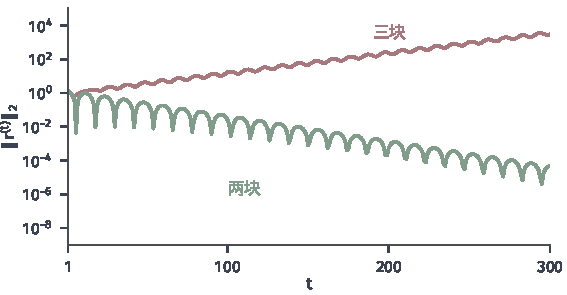
\includegraphics[width=96mm]{figures/05-optimization/06-constrained-optimization/matplotlib/pm-admm-threeblock/figure.pdf}
  \caption{同一个线性系统上的三块与两块ADMM，$\rho=1$，半对数坐标，初值$\bm{x}^{(0)}=(1,1,1)$，乘子初值为零。红线是逐块更新三块的残差，发散；绿线把后两块合并成一块，收敛。}
  \label{fig:pm-admm-threeblock}
\end{BookInlineFigure}

非凸问题上的ADMM使用很广，但一般只能保证在额外的结构条件下收敛到驻点，有时需要$\rho$足够大，有时根本不收敛。一个非凸改写在形式上和ADMM相同，并不意味着上面的定理适用，每种情形都需要重新分析。结束时仍然要回到原约束和最优性条件上去检查。

\section{方法比较与计算成本}
\label{sec:pm-comparison}

本节回答一个实际问题：同一个约束问题，四种方法到底哪里不同，比较代价时应该数什么。

\paragraph{各方法改变了什么}
四种方法都在做同一件事，把约束的信息换成原始变量子问题里的一项。它们的差别可以按三个方面读出来：给目标加了什么，乘子怎样更新，原始变量怎样求解。

\begin{BookInlineTable}
  \centering
  \small
  \begin{tabular}{@{}llll@{}}
    \toprule
    方法 & 目标的改动 & 乘子 & 原始变量\\
    \midrule
    二次罚 & 加平方罚 & 无（$\rho h$仅作估计） & 逐轮全部求解\\
    一次罚 & 加一次罚 & 无（门槛内隐含） & 非光滑子问题\\
    对偶上升 & 加线性价格 & 显式步 & 可分块，全部求解\\
    ALM & 价格加平方罚 & 隐式步，步长$\rho$ & 联合求解\\
    ADMM & 价格加平方罚 & 步长$\rho$ & 两块各更新一次\\
    \bottomrule
  \end{tabular}
  \caption{各方法的结构对照。}
  \label{tab:pm-structure}
\end{BookInlineTable}

\paragraph{相同精度下的代价}
比较时要固定口径。各方法的罚目标函数不同，比较目标值没有意义；ADMM的一轮和ALM的一轮完成的工作也不同，比较轮数同样没有意义。合理的办法是固定同一个问题，要求达到相同的原始精度，再分别统计外层轮数、内层计算和通信。

下面用二元例，都从原点出发，要求$\lvert h(\bm{x})\rvert\leq10^{-3}$。内层的梯度法取步长$1/L$，容差为$10^{-6}$，这样内层误差不干扰外层。ADMM的两个子问题都是一元二次函数的最小化，取闭式解。

\begin{BookInlineTable}
  \centering
  \small
  \begin{tabular}{@{}lrrrr@{}}
    \toprule
    方法 & 外层轮数 & 内层梯度步 & 矩阵分解 & 最大条件数\\
    \midrule
    二次罚（$\rho$乘$10$） & $5$ & $123443$ & $5$ & $15001$\\
    对偶上升（$\alpha=0.6$） & $7$ & $162$ & $0$ & $3$\\
    ALM（$\rho=1.5$） & $8$ & $230$ & $1$ & $3.1$\\
    ADMM（$\rho=1.5$） & $11$ & 闭式 & $0$ & 无\\
    \bottomrule
  \end{tabular}
  \caption{二元例中达到$\lvert h\rvert\leq10^{-3}$的代价。“矩阵分解”指改用直接法解内层时需要的分解次数。这些数字只对这个例子有效。}
  \label{tab:pm-cost}
\end{BookInlineTable}

表~\ref{tab:pm-cost}和图~\ref{fig:pm-compare}说明了几件事。二次罚外层轮数最少，内层步数却多出几个数量级，几乎全部花在最后两轮的病态问题上。ALM比二次罚多几轮，却始终在解同一个良态问题。

对偶上升在这里表现很好，因为$f$是强凸的，内层矩阵的条件数只有$3$，步长也事先选好了。如果把目标改成线性的，或者步长取到$1.5$，它就失效了，表中的数字不能外推。ADMM在这里每个子问题都是一元的，所以一轮很便宜，但一轮要交换一次信息。在通信比本地计算贵得多的环境中，轮数才是主要成本。

\begin{BookInlineFigure}
  \centering
  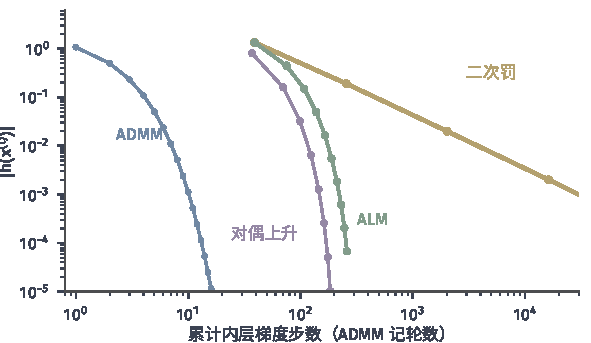
\includegraphics[width=100mm]{figures/05-optimization/06-constrained-optimization/matplotlib/pm-compare/figure.pdf}
  \caption{二元例上约束残差随累计计算量的下降，双对数坐标。黄线是二次罚，紫线是对偶上升，绿线是ALM，横轴是累计的梯度步数（内层容差$10^{-6}$）；蓝线是ADMM，横轴是轮数，两者的单位不同，只宜比较曲线的走势。}
  \label{fig:pm-compare}
\end{BookInlineFigure}

\paragraph{比较时容易出错的地方}
第一，不同方法的罚目标值不可比。$Q_\rho$、$E_\rho$、$\mathcal{L}_\rho$的数值里都混有罚项，要比较的是原目标和约束违规，或者驻定残差。

第二，只比较一次内层更新的速度会误导。一次梯度步的时间四种方法差不多，但需要多少步完全取决于子问题的条件数；对偶上升的内层便宜，可能需要更多外层轮数。

第三，精度要对等。一个方法返回约束残差$10^{-3}$的点，另一个返回$10^{-6}$的点，前者的目标值可能因为更不可行而显得更低。

第四，不同方法适用的问题不同，这个例子凸、光滑、约束线性。约束非线性时，对偶上升和ADMM的结论都要重新检查；目标非凸时，ALM的局部结论才是相关的。选择方法时应先看问题的结构：约束少而目标规模大时考虑ALM，目标和约束可分时考虑对偶分解或ADMM，只需要中等精度且子问题便宜时考虑ADMM，需要高精度时考虑ALM或者后面两章的方法。

\section{本章小结}
\label{sec:pm-summary}

本章从一个问题开始：允许迭代点暂时违反约束，用什么信号把它拉回来。

惩罚方法给违规计价。二次罚光滑，但边界上没有回推的力，有限的$\rho$总留下违规，$\rho\to\infty$时法向曲率随之增长，子问题越来越病态。一次罚在边界上有尖角，$\rho$超过最优乘子的最大绝对分量后最小点就是原问题的解，代价是目标不可微。“精确”的含义是解的对应，全局结论需要强对偶和对偶解存在，局部结论需要误差界或二阶条件。

对偶上升直接调整价格。解完Lagrange子问题，约束残差就是对偶函数的超梯度，目标可分时各块可以独立求解。它改进的是下界，迭代点通常不可行，步长受限，$q$不可微时单步未必上升；要得到原始解，需要平均、选解或修复，并且同时报告可行性和间隙。

增广Lagrange法把价格和平方罚合在一起。乘子提供大部分的力，罚项修正余下的部分，所以有限的$\rho$就够了。从对偶问题看，它是隐式的邻近点步，比显式的对偶上升稳定得多，凸问题中任何固定的$\rho>0$都收敛。代价是平方项把变量耦合起来，子问题更难。不等式要用正部形式，乘子要保持非负。

ADMM把两块变量各更新一次，用一次乘子更新代替联合求解。这样既保留乘子的稳定性，又能分别利用两块结构，代价是出现了对偶残差。原始残差和对偶残差要一起看，$\rho$改变时缩放乘子要同步换算。两块闭凸目标在鞍点存在时有收敛保证，多块或非凸的情形不能沿用。

\begin{BookInlineTable}
  \centering
  \small
  \begin{tabular}{@{}lll@{}}
    \toprule
    方法 & 主要条件 & 能保证什么\\
    \midrule
    二次罚 & 各轮全局解，$\rho\to\infty$ & 聚点全局最优\\
    一次罚 & 强对偶，$\rho$超过门槛 & 最小点集合相同\\
    对偶上升 & 残差来自全局最小点 & 超梯度；凸时平均点渐近可行\\
    ALM & 凸，强对偶，固定$\rho$ & 残差趋零，目标值收敛\\
    ADMM & 两块闭凸，鞍点存在 & 两种残差趋零，目标值收敛\\
    \bottomrule
  \end{tabular}
  \caption{本章各方法的主要条件与保证。局部结论和近似求解下的结论见各节。}
  \label{tab:pm-summary}
\end{BookInlineTable}

几种方法结束时要做的事是一样的：回到原约束检查可行性，回到Lagrange函数检查驻定，有不等式时检查互补；需要全局结论时，再用对偶值或者凸性给出证书。第~\ref{chap:sequential-quadratic-programming}章接着处理光滑非线性约束，用局部二次模型同时更新原始变量和乘子。


\chapter{序列二次规划}
\label{chap:sequential-quadratic-programming}

考虑圆周上的一个小问题：
\begin{equation}
 \min_{\bm{x}\in\mathbb{R}^2}\ f(\bm{x})=-x_1-x_2
 \quad\text{s.t.}\quad h(\bm{x})=x_1^2+x_2^2-2=0.
 \label{eq:sqp-circle}
\end{equation}
解是$\bm{x}^\star=(1,1)^\top$。第~\ref{chap:penalty-multiplier-methods}章的办法是把约束折进目标，解一串无约束问题，每个无约束问题自身又要迭代很多步。第~\ref{chap:second-order-methods}章的Newton法提示了另一条路：在当前点建一个局部模型，一步解出模型的最优步，再换一个点重建模型。

把这个想法搬到约束问题上，立刻有几个问题。约束也要进入模型，它该近似到几阶？式~\eqref{eq:sqp-circle}的目标是线性的，Hessian为零，模型的曲率从哪里来？约束不止一条时，哪些不等式此刻该算数？模型给出的步不满足真实约束，也未必降低目标，又凭什么采用它？

本章按这个顺序回答。第~\ref{sec:sqp-local-model}节写出局部模型，它是一个二次规划。第~\ref{sec:sqp-equality-qp}节解只含等式的模型，第~\ref{sec:sqp-active-set}节处理不等式。第~\ref{sec:sqp-curvature}节讨论模型的曲率不合适时怎么办。

第~\ref{sec:sqp-acceptance}节把模型的步放回原问题检验，第~\ref{sec:sqp-repair}节处理模型本身失效或好步被误拒的情形。第~\ref{sec:sqp-convergence}节说明这些部件合起来在什么条件下收敛得快，以及每一轮要花多少计算。全章用问题~\eqref{eq:sqp-circle}作手算的主线。

\section{局部二次模型}
\label{sec:sqp-local-model}

站在当前点$\bm{x}^{(t)}$，怎样写出一个既能求解、又能代表原问题的局部模型？一般的问题写成
\begin{equation}
 \begin{aligned}
 \min_{\bm{x}\in\mathbb{R}^n}\quad & f(\bm{x})\\
 \text{s.t.}\quad & g_i(\bm{x})\leq0,\quad i=1,\ldots,m,\\
 & h_j(\bm{x})=0,\quad j=1,\ldots,p,
 \end{aligned}
 \label{eq:sqp-nlp}
\end{equation}
其中$f,g_i,h_j$都二阶连续可微。

\paragraph{约束怎样近似}
Newton法把目标近似到二阶。约束若也近似到二阶，模型的可行域由二次曲面围成，这样的子问题本身就难解。所以约束只取一阶，用切平面代替曲面。记$\bm{d}$为待求的步，把约束的值和梯度在$\bm{x}^{(t)}$处取定，有
\[
 h_j(\bm{x}^{(t)}+\bm{d})\approx h_j(\bm{x}^{(t)})+\langle\nabla h_j(\bm{x}^{(t)}),\bm{d}\rangle.
\]

把各条约束的梯度按行排成Jacobian矩阵，记$\bm{A}^{(t)}\in\mathbb{R}^{p\times n}$的第$j$行为$\nabla h_j(\bm{x}^{(t)})^\top$，$\bm{G}^{(t)}\in\mathbb{R}^{m\times n}$的第$i$行为$\nabla g_i(\bm{x}^{(t)})^\top$。约束的值记作向量$\bm{h}^{(t)}$和$\bm{g}^{(t)}$。这样，要求线性化后的约束成立就是
\begin{equation}
 \bm{h}^{(t)}+\bm{A}^{(t)}\bm{d}=\bm{0},\qquad \bm{g}^{(t)}+\bm{G}^{(t)}\bm{d}\leq\bm{0}.
 \label{eq:sqp-linearized}
\end{equation}

以问题~\eqref{eq:sqp-circle}为例，从$\bm{x}^{(0)}=(1.5,0.5)^\top$出发。约束的值和梯度是
\[
 h^{(0)}=2.25+0.25-2=0.5,\qquad \bm{A}^{(0)}=(3,1).
\]

线性化约束于是成为
\[
 3d_1+d_2+0.5=0.
\]
图~\ref{fig:sqp-circle-model}(a)中的虚线就是这条直线。$\bm{x}^{(0)}$在圆外，过它有一条等值线$h=0.5$。虚线与这条等值线在$\bm{x}^{(0)}$处的切线平行，并向圆的方向平移，平移量按一阶估计恰好抵消$h^{(0)}=0.5$的违约。

\begin{BookInlineFigure}
 \centering
 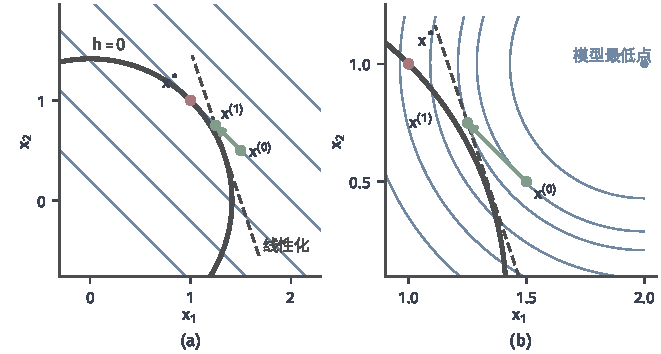
\includegraphics[width=112mm]{figures/05-optimization/06-constrained-optimization/matplotlib/sqp-circle-model/figure.pdf}
 \caption{问题~\eqref{eq:sqp-circle}的第一个局部模型。深灰粗线是圆$h=0$，虚线是线性化约束，绿点是迭代点，红点是解。(a)~蓝色直线是目标的等值线，步落在虚线上而不在圆上。(b)~放大的局部，蓝色圆是取$\bm{B}^{(0)}=2\bm{I}$时模型的等值线，模型无约束的最低点在右上方，受虚线限制后，最优步停在等值线与虚线相切的地方。}
 \label{fig:sqp-circle-model}
\end{BookInlineFigure}

\paragraph{目标怎样近似}
目标的一阶项仍取$\langle\nabla f(\bm{x}^{(t)}),\bm{d}\rangle$，二次项用一个对称矩阵$\bm{B}^{(t)}$。把两部分合起来，就得到局部模型。下面的定义里$\bm{B}^{(t)}$暂时留作待定，它的选取马上讨论。

\begin{definition}[局部二次规划与SQP]
\label{def:sqp-subproblem}
给定当前点$\bm{x}^{(t)}$与对称矩阵$\bm{B}^{(t)}$，\term{局部二次规划}（local quadratic program）是以$\bm{d}\in\mathbb{R}^n$为未知量的问题
\begin{equation}
 \begin{aligned}
 \min_{\bm{d}}\quad & \langle\nabla f(\bm{x}^{(t)}),\bm{d}\rangle+\frac12\bm{d}^\top\bm{B}^{(t)}\bm{d}\\
 \text{s.t.}\quad & \bm{h}^{(t)}+\bm{A}^{(t)}\bm{d}=\bm{0},\\
 & \bm{g}^{(t)}+\bm{G}^{(t)}\bm{d}\leq\bm{0}.
 \end{aligned}
 \label{eq:sqp-qp}
\end{equation}
反复构造并求解这样的子问题、用其解更新迭代点和乘子的方法，称为\term{序列二次规划}（sequential quadratic programming，SQP）。
\end{definition}

目标是二次的、约束是线性的，这就是第~\ref{chap:quadratic-conic-programming}章的二次规划（QP）。每一项的职责不同：目标梯度指出一阶意义下该往哪里走；$\bm{h}^{(t)},\bm{g}^{(t)}$说明当前违约多少；两个Jacobian说明约束怎样随步变化；$\bm{B}^{(t)}$说明走远了之后模型该怎样弯曲。

\paragraph{曲率为什么不能只取目标的Hessian}
最自然的想法是令$\bm{B}^{(t)}=\nabla^2f(\bm{x}^{(t)})$。式~\eqref{eq:sqp-circle}直接否定了这个想法。这里$\nabla^2f=\bm{0}$，模型的目标退化成线性函数，而可行集是一条直线，只要目标沿这条直线的斜率不为零，模型就没有下界。可是真实问题在圆上明明有一个弯曲的碗。

这只碗来自约束的弯曲。设想沿圆周走：坐标$x_1,x_2$本身在转弯，所以线性函数$f$沿圆周读出来的数值是弯的。模型把圆拉直成了直线，这部分弯曲必须另外算回目标的二次项。

下面把这件事算清楚。设$\bm{x}(s)$是一条留在等式约束上的光滑曲线，它在$s=0$处经过$\bm{x}$，速度是$\bm{v}$，加速度是$\bm{w}$。对恒等式$h_j(\bm{x}(s))=0$在$s=0$处求两次导数，得到
\[
 \langle\nabla h_j(\bm{x}),\bm{v}\rangle=0,\qquad
 \langle\nabla h_j(\bm{x}),\bm{w}\rangle+\bm{v}^\top\nabla^2h_j(\bm{x})\bm{v}=0.
\]

目标沿这条曲线的二阶导数由链式法则给出，它含有加速度$\bm{w}$：
\[
 \frac{\mathrm{d}^2}{\mathrm{d}s^2}f(\bm{x}(s))\Big|_{s=0}
 =\bm{v}^\top\nabla^2f(\bm{x})\bm{v}+\langle\nabla f(\bm{x}),\bm{w}\rangle.
\]

第~\ref{chap:constrained-optimality}章的一阶条件说，KKT点上$\nabla f+\sum_j\nu_j\nabla h_j=\bm{0}$，这里记Lagrange函数为$\mathcal{L}=f+\sum_i\lambda_ig_i+\sum_j\nu_jh_j$。把$\nabla f$代换掉，再用前面关于$\bm{w}$的恒等式，得到
\[
 \langle\nabla f,\bm{w}\rangle=-\sum_j\nu_j\langle\nabla h_j,\bm{w}\rangle=\sum_j\nu_j\bm{v}^\top\nabla^2h_j\bm{v}.
\]

代回上式，加速度消失了，剩下的正是Lagrange函数的Hessian：
\begin{equation}
 \frac{\mathrm{d}^2}{\mathrm{d}s^2}f(\bm{x}(s))\Big|_{s=0}
 =\bm{v}^\top\nabla^2_{\bm{x}\bm{x}}\mathcal{L}(\bm{x},\bm{\nu})\bm{v}.
 \label{eq:sqp-curve-curvature}
\end{equation}
这里乘子把约束的弯曲折算成了目标的弯曲，它正是第~\ref{chap:constrained-optimality}章二阶条件里出现$\nabla^2_{\bm{x}\bm{x}}\mathcal{L}$的原因。活动的不等式在其边界上同样处理，不活动的不等式乘子为零，不贡献曲率。

在圆上验证一下。沿圆取弧长参数$s$，解$\bm{x}^\star$处的乘子由$(-1,-1)^\top+\nu(2,2)^\top=\bm{0}$得$\nu^\star=1/2$，于是
\[
 \nabla^2_{\bm{x}\bm{x}}\mathcal{L}=2\nu^\star\bm{I}=\bm{I}.
\]

单位切向量$\bm{v}$给出$\bm{v}^\top\bm{I}\bm{v}=1$。另一方面，沿圆有$f=-2\cos(s/\sqrt2)$，它在$s=0$处的二阶导数是
\[
 \frac{\mathrm{d}^2f}{\mathrm{d}s^2}\Big|_{s=0}=2\cdot\frac12=1,
\]
两者相等。图~\ref{fig:sqp-curvature-circle}(a)画的就是这件事：带Lagrange曲率的模型与圆上的目标贴合，只用$\nabla^2f$的模型是一条平线。

\begin{BookInlineFigure}
 \centering
 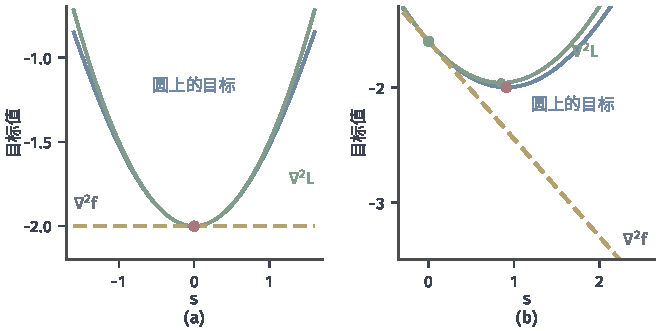
\includegraphics[width=112mm]{figures/05-optimization/06-constrained-optimization/matplotlib/sqp-curvature-along-circle/figure.pdf}
 \caption{沿约束的目标与两种模型，$s$是弧长（对模型是沿切线的距离）。蓝线是圆上真实的目标；绿线的二次项取$\nabla^2_{\bm{x}\bm{x}}\mathcal{L}=\bm{I}$；黄色虚线的二次项取$\nabla^2f=\bm{0}$。(a)~在解$\bm{x}^\star$处（红点）。(b)~在圆上的点$(1.4,0.2)^\top$处（左侧绿点）：绿色模型的最低点靠近真实最低点，只用$\nabla^2f$的模型沿切线一路下降，没有下界。}
 \label{fig:sqp-curvature-circle}
\end{BookInlineFigure}

式~\eqref{eq:sqp-curve-curvature}的推导用到了KKT点上的梯度关系，所以严格说它是解处的性质。迭代中手里只有估计值，于是取
\begin{equation}
 \bm{B}^{(t)}=\nabla^2_{\bm{x}\bm{x}}\mathcal{L}(\bm{x}^{(t)},\bm{\lambda}^{(t)},\bm{\nu}^{(t)})
 =\nabla^2f+\sum_{i=1}^m\lambda_i^{(t)}\nabla^2g_i+\sum_{j=1}^p\nu_j^{(t)}\nabla^2h_j,
 \label{eq:sqp-lagrangian-hessian}
\end{equation}
右端都在$\bm{x}^{(t)}$处取值，或取它的近似（第~\ref{sec:sqp-quasi-newton}节）。这解释了SQP为什么要同时维护原始变量和乘子：没有乘子，就写不出模型的曲率。

图~\ref{fig:sqp-curvature-circle}(b)显示了乘子估计不太准时的情形。点$(1.4,0.2)^\top$在圆上但不是解，取$\nu=1/2$，绿色模型的最低点仍然靠近真实的最低点。类比“局部模型信多远”：线性化约束告诉我们该待在哪里，乘子曲率告诉我们沿着允许的方向能走多远。这个类比在远离解时失效，那时乘子可能是错的，模型未必是碗，这是第~\ref{sec:sqp-curvature}节的话题。

\paragraph{子问题的乘子}
QP也有自己的乘子。记不等式的乘子为$\hat{\bm{\lambda}}$，等式的乘子为$\hat{\bm{\nu}}$。线性约束本身满足约束资格，所以把第~\ref{chap:constrained-optimality}章的KKT条件用于式~\eqref{eq:sqp-qp}时，它的每个局部解都满足
\begin{equation}
 \begin{gathered}
 \bm{B}^{(t)}\bm{d}+\nabla f(\bm{x}^{(t)})+(\bm{A}^{(t)})^\top\hat{\bm{\nu}}+(\bm{G}^{(t)})^\top\hat{\bm{\lambda}}=\bm{0},\\
 \bm{h}^{(t)}+\bm{A}^{(t)}\bm{d}=\bm{0},\qquad \bm{g}^{(t)}+\bm{G}^{(t)}\bm{d}\leq\bm{0},\\
 \hat{\bm{\lambda}}\geq\bm{0},\qquad \hat\lambda_i\bigl(g_i^{(t)}+\langle\nabla g_i^{(t)},\bm{d}\rangle\bigr)=0,\quad i=1,\ldots,m.
 \end{gathered}
 \label{eq:sqp-qp-kkt}
\end{equation}

把$\bm{d}=\bm{0}$代入式~\eqref{eq:sqp-qp-kkt}，第一行成为原问题的Lagrange驻定条件，第二行成为原问题的可行性，第三行成为原问题的乘子非负与互补。这就是下面的引理，它说明模型和原问题在解处是一致的。

\begin{lemma}[零步与KKT点]
\label{lem:sqp-zero-step}
$\bm{d}=\bm{0}$连同乘子$(\hat{\bm{\lambda}},\hat{\bm{\nu}})$满足式~\eqref{eq:sqp-qp-kkt}，当且仅当$(\bm{x}^{(t)},\hat{\bm{\lambda}},\hat{\bm{\nu}})$满足原问题~\eqref{eq:sqp-nlp}的KKT条件。
\end{lemma}

\begin{proof}
令$\bm{d}=\bm{0}$，含$\bm{B}^{(t)}$的项消失，线性化项都等于在$\bm{x}^{(t)}$处的取值。式~\eqref{eq:sqp-qp-kkt}逐行就是原问题在$\bm{x}^{(t)}$处的驻定、可行、乘子非负和互补条件，反过来也一样。
\end{proof}

引理与$\bm{B}^{(t)}$无关，所以不论曲率怎样近似，模型的不动点都是原问题的KKT点。曲率只影响走向这个点的速度。解完QP后，新的乘子估计可以直接取子问题的乘子，当步长$\alpha^{(t)}\in(0,1]$时按比例插值：
\begin{equation}
 \begin{aligned}
 \bm{\lambda}^{(t+1)}&=\bm{\lambda}^{(t)}+\alpha^{(t)}\bigl(\hat{\bm{\lambda}}-\bm{\lambda}^{(t)}\bigr),\\
 \bm{\nu}^{(t+1)}&=\bm{\nu}^{(t)}+\alpha^{(t)}\bigl(\hat{\bm{\nu}}-\bm{\nu}^{(t)}\bigr).
 \end{aligned}
 \label{eq:sqp-multiplier-update}
\end{equation}

\paragraph{一轮计算的结构}
图~\ref{fig:sqp-loop}把一轮计算的部件排在一起。求值之后得到子问题，子问题给出步和乘子，步还要放回原问题检验。两处可能出岔：子问题可能无解，步也可能被拒绝。后面各节依次处理这些部件。

\begin{BookInlineFigure}
 \centering
 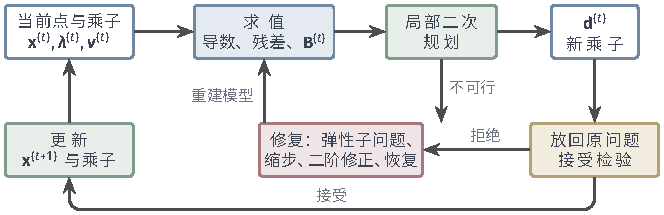
\includegraphics[width=112mm]{figures/05-optimization/06-constrained-optimization/tikz/sqp-loop/figure.pdf}
 \caption{SQP一轮计算的结构。绿框是模型的构造与接受后的更新，黄框是把步放回非线性问题的检验，红框是子问题无解或候选步被拒绝时的修复。修复之后重新建模或重新求解。}
 \label{fig:sqp-loop}
\end{BookInlineFigure}

需要说明的是，SQP规定的是“解一列局部QP”，并没有规定用什么方法解QP。下面用有效集法讲解，因为它的逻辑最贴近“哪些约束算数”这个问题；QP也可以用内点法或其他方法求解，第~\ref{chap:nonlinear-interior-point}章的内点法思想同样适用于QP。

局部模型还有一点要记住：模型可行不等于原问题可行。式~\eqref{eq:sqp-linearized}只是切平面，步$\bm{d}$落在切平面上，一般不在原来的曲面上。这个缺口贯穿全章，第~\ref{sec:sqp-acceptance}节和第~\ref{sec:sqp-repair}节专门处理它。

\section{等式QP的求解}
\label{sec:sqp-equality-qp}

式~\eqref{eq:sqp-qp}只含等式时，怎样求出它的解，这个解又在什么条件下才算数？这是SQP最基本的一步，下一节处理不等式时，每一轮要解的也是这种问题。为减少上标，本节在不引起混淆时省去$(t)$，并记$\bm{g}=\nabla f(\bm{x}^{(t)})$。

\paragraph{KKT线性系统}
只含等式时，条件~\eqref{eq:sqp-qp-kkt}的第一、二行就是全部要求。它们对$(\bm{d},\hat{\bm{\nu}})$是线性的，合起来写成块方程
\begin{equation}
 \underbrace{\begin{bmatrix}\bm{B}&\bm{A}^\top\\\bm{A}&\bm{0}\end{bmatrix}}_{\bm{K}}
 \begin{bmatrix}\bm{d}\\\hat{\bm{\nu}}\end{bmatrix}
 =-\begin{bmatrix}\bm{g}\\\bm{h}\end{bmatrix}.
 \label{eq:sqp-kkt-system}
\end{equation}
矩阵$\bm{K}\in\mathbb{R}^{(n+p)\times(n+p)}$称为\term{KKT矩阵}（KKT matrix）。它对称但不定，零对角块使它不可能正定，所以不能用Cholesky分解。

这个方程有解并不等于模型有最小点。要回答后一个问题，得看$\bm{B}$在允许的方向上是否向上弯。允许的方向是满足$\bm{A}\bm{v}=\bm{0}$的方向，它们构成$\bm{A}$的零空间。取矩阵$\bm{Z}\in\mathbb{R}^{n\times(n-p)}$，其各列构成这个零空间的一组基，就把问题缩到这$n-p$维上。矩阵$\bm{Z}^\top\bm{B}\bm{Z}$称为\term{约化Hessian}（reduced Hessian）。

\begin{theorem}[等式QP的可解性]
\label{thm:sqp-eqp}
设$\bm{A}\in\mathbb{R}^{p\times n}$行满秩，$\bm{Z}$的各列是其零空间的一组基，且$\bm{Z}^\top\bm{B}\bm{Z}\succ\bm{0}$。则$\bm{K}$可逆，方程~\eqref{eq:sqp-kkt-system}有唯一解$(\bm{d},\hat{\bm{\nu}})$，并且$\bm{d}$是等式QP唯一的全局最小点。
\end{theorem}

\begin{proof}
先证$\bm{K}$可逆。设$\bm{K}(\bm{u}^\top,\bm{w}^\top)^\top=\bm{0}$，即$\bm{B}\bm{u}+\bm{A}^\top\bm{w}=\bm{0}$且$\bm{A}\bm{u}=\bm{0}$。

用$\bm{u}^\top$左乘第一式，并用$\bm{A}\bm{u}=\bm{0}$消去含$\bm{w}$的项，得到
\[
 \bm{u}^\top\bm{B}\bm{u}=0.
\]

由$\bm{A}\bm{u}=\bm{0}$可写$\bm{u}=\bm{Z}\bm{z}$，代入上式得到
\[
 \bm{z}^\top\bm{Z}^\top\bm{B}\bm{Z}\bm{z}=0.
\]

约化Hessian正定，所以$\bm{z}$和$\bm{u}$都是零向量。第一式于是成为$\bm{A}^\top\bm{w}=\bm{0}$，$\bm{A}$行满秩给出$\bm{w}=\bm{0}$。

再证最小性。设$\bar{\bm{d}}$是任一可行步，令$\bm{v}=\bar{\bm{d}}-\bm{d}$，则$\bm{A}\bm{v}=\bm{0}$。记目标为$q$，展开得
\[
 q(\bar{\bm{d}})-q(\bm{d})=\langle\bm{g}+\bm{B}\bm{d},\bm{v}\rangle+\frac12\bm{v}^\top\bm{B}\bm{v}.
\]

由方程第一行，$\bm{g}+\bm{B}\bm{d}=-\bm{A}^\top\hat{\bm{\nu}}$，它与$\bm{v}$正交，第一项为零。所以
\[
 q(\bar{\bm{d}})-q(\bm{d})=\frac12\bm{v}^\top\bm{B}\bm{v}.
\]
$\bm{v}\neq\bm{0}$时$\bm{v}=\bm{Z}\bm{z}$且$\bm{z}\neq\bm{0}$，右端为正。
\end{proof}

两个条件各有分工。行满秩保证约束不互相矛盾、乘子唯一：若$\bm{A}$有一行是另一行的倍数而右端不相称，线性化约束根本无解，这种情形留到第~\ref{sec:sqp-restoration}节。约化Hessian正定保证驻点是最小点，它只要求$\bm{B}$在$n-p$个允许的方向上正定，不要求$\bm{B}$在全空间正定，第~\ref{sec:sqp-curvature}节会看到两者的差别。

\paragraph{直接解鞍点方程}
第一种做法是把$\bm{K}$当作一个$(n+p)$阶的对称不定矩阵，做带主元的$\bm{L}\bm{D}\bm{L}^\top$分解后回代。它一次同时给出$\bm{d}$和$\hat{\bm{\nu}}$，也能保持稀疏性，是大规模稀疏问题的常用选择。

小问题可以手算，办法是先消去$\bm{d}$。回到第一个模型，取$\bm{\nu}^{(0)}=1$，于是$\bm{B}=2\nu^{(0)}\bm{I}=2\bm{I}$，数据是
\[
 \bm{g}=(-1,-1)^\top,\qquad h=0.5,\qquad \bm{A}=(3,1).
\]

方程~\eqref{eq:sqp-kkt-system}的第一行给出$\bm{d}$关于$\hat\nu$的表达式：
\[
 \bm{d}=-\frac12\bigl(\bm{g}+\hat\nu\bm{A}^\top\bigr)=\frac12\begin{bmatrix}1-3\hat\nu\\1-\hat\nu\end{bmatrix}.
\]

代入第二行$\bm{A}\bm{d}=-h$，左端是$\frac12(3-9\hat\nu+1-\hat\nu)=2-5\hat\nu$，于是
\[
 2-5\hat\nu=-0.5,\qquad\text{即}\qquad\hat\nu=0.5.
\]

再代回$\bm{d}$的表达式，得到
\[
 \bm{d}=(-0.25,\ 0.25)^\top.
\]
这就是图~\ref{fig:sqp-circle-model}中的绿色箭头。

\paragraph{在零空间中求解}
第二种做法把步分成两段，分别完成两件事。第一段让线性化约束成立，第二段在不破坏它的前提下降低模型。取$\bm{Y}\in\mathbb{R}^{n\times p}$使$\bm{A}\bm{Y}$可逆，把步写成
\begin{equation}
 \bm{d}=\bm{Y}\bm{d}_Y+\bm{Z}\bm{d}_Z.
 \label{eq:sqp-range-null}
\end{equation}

因为$\bm{A}\bm{Z}=\bm{0}$，约束$\bm{A}\bm{d}=-\bm{h}$只约束$\bm{d}_Y$，得到$p$维的方程
\begin{equation}
 \bm{A}\bm{Y}\bm{d}_Y=-\bm{h}.
 \label{eq:sqp-normal-step}
\end{equation}

固定$\bm{d}_Y$，把式~\eqref{eq:sqp-range-null}代入目标，对$\bm{d}_Z$求最小，就是$n-p$维的无约束二次问题，其驻点方程为
\begin{equation}
 \bm{Z}^\top\bm{B}\bm{Z}\,\bm{d}_Z=-\bm{Z}^\top\bigl(\bm{g}+\bm{B}\bm{Y}\bm{d}_Y\bigr).
 \label{eq:sqp-reduced-step}
\end{equation}

最后，方程~\eqref{eq:sqp-kkt-system}的第一行左乘$\bm{Y}^\top$，就解出乘子：
\begin{equation}
 (\bm{A}\bm{Y})^\top\hat{\bm{\nu}}=-\bm{Y}^\top\bigl(\bm{g}+\bm{B}\bm{d}\bigr).
 \label{eq:sqp-null-multiplier}
\end{equation}

继续用同一组数据。取$\bm{Y}=\bm{A}^\top=(3,1)^\top$，此时$\bm{A}\bm{Y}=10$，再取$\bm{Z}=(1,-3)^\top$，可以核对$\bm{A}\bm{Z}=0$。由式~\eqref{eq:sqp-normal-step}，
\[
 d_Y=-\frac{0.5}{10}=-0.05,\qquad \bm{Y}d_Y=(-0.15,\ -0.05)^\top.
\]

计算式~\eqref{eq:sqp-reduced-step}的两边。约化Hessian是$\bm{Z}^\top\bm{B}\bm{Z}=2\times10=20$，右端需要的向量和内积是
\[
 \bm{g}+\bm{B}\bm{Y}d_Y=(-1.3,\ -1.1)^\top,\qquad
 \bm{Z}^\top(\bm{g}+\bm{B}\bm{Y}d_Y)=-1.3+3.3=2.
\]

于是
\[
 d_Z=-\frac{2}{20}=-0.1,\qquad \bm{Z}d_Z=(-0.1,\ 0.3)^\top.
\]

两段相加，得到$\bm{d}=(-0.25,0.25)^\top$，和直接解法一致。用式~\eqref{eq:sqp-null-multiplier}求乘子，先算$\bm{g}+\bm{B}\bm{d}=(-1.5,-0.5)^\top$，于是
\[
 10\,\hat\nu=-(3,1)\begin{bmatrix}-1.5\\-0.5\end{bmatrix}=5,\qquad\hat\nu=0.5.
\]

图~\ref{fig:sqp-range-null}是这两段的几何。紫色的一段垂直于虚线，它只管把点送到线性化约束上；黄色的一段沿虚线走，它只管沿允许的方向降低模型，这里的$\bm{Z}$就是把“沿虚线走多少”变成$\mathbb{R}^2$中位移的那个矩阵。

\begin{BookInlineFigure}
 \centering
 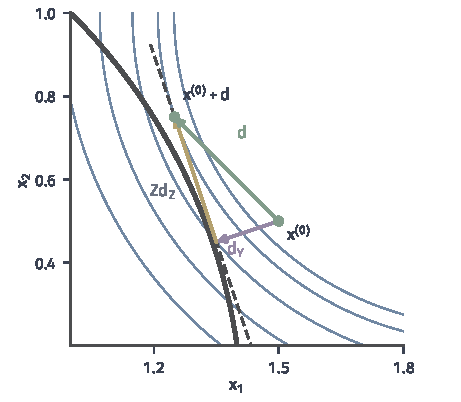
\includegraphics[width=78mm]{figures/05-optimization/06-constrained-optimization/matplotlib/sqp-range-null/figure.pdf}
 \caption{第一个局部模型的两段分解。深灰粗线是圆，虚线是线性化约束，蓝线是模型的等值线。紫色$\bm{Y}d_Y$从$\bm{x}^{(0)}$走到虚线，黄色$\bm{Z}d_Z$沿虚线走到模型的条件最小点，两段之和是绿色的$\bm{d}$。}
 \label{fig:sqp-range-null}
\end{BookInlineFigure}

\begin{BookInlineTable}
 \centering
 \begin{tabular}{lll}
  \toprule
  比较项 & 解KKT系统 & 零空间方法\\
  \midrule
  分解对象 & $(n+p)$阶对称不定 & $\bm{A}$的分解与$n-p$阶约化矩阵\\
  $n-p$很小时 & 仍解$n+p$阶 & 约化矩阵很小，便宜\\
  稀疏性 & 容易保持 & $\bm{Z}$可能变稠密\\
  检查曲率 & 需看分解的惯性 & 直接检查约化矩阵\\
  \bottomrule
 \end{tabular}
 \caption{等式QP两种解法的比较。}
 \label{tab:sqp-eqp-methods}
\end{BookInlineTable}

\paragraph{与原问题Newton步的关系}
到这里，KKT系统还只是模型的条件。现在换一个角度，从原问题出发。只含等式时，原问题的KKT条件是非线性方程组
\begin{equation}
 \bm{F}(\bm{x},\bm{\nu})=\begin{bmatrix}\nabla f(\bm{x})+\bm{A}(\bm{x})^\top\bm{\nu}\\\bm{h}(\bm{x})\end{bmatrix}=\bm{0}.
 \label{eq:sqp-kkt-map}
\end{equation}
自然的想法是对这个方程组直接用Newton法。下面的定理说，这和解局部QP是同一件事。

\begin{theorem}[SQP与KKT方程的Newton法]
\label{thm:sqp-newton}
设$\bm{B}$取Lagrange函数在$(\bm{x},\bm{\nu})$处对$\bm{x}$的Hessian。则$(\bm{\delta}_x,\bm{\delta}_\nu)$是$\bm{F}$在$(\bm{x},\bm{\nu})$处的Newton步，当且仅当$\bm{d}=\bm{\delta}_x$，$\hat{\bm{\nu}}=\bm{\nu}+\bm{\delta}_\nu$满足方程~\eqref{eq:sqp-kkt-system}。
\end{theorem}

\begin{proof}
$\bm{F}$的第一块对$\bm{x}$的导数是$\nabla^2_{\bm{x}\bm{x}}\mathcal{L}=\bm{B}$，对$\bm{\nu}$的导数是$\bm{A}^\top$；第二块对$\bm{x}$的导数是$\bm{A}$，对$\bm{\nu}$的导数为零。所以Newton方程是
\[
 \begin{bmatrix}\bm{B}&\bm{A}^\top\\\bm{A}&\bm{0}\end{bmatrix}
 \begin{bmatrix}\bm{\delta}_x\\\bm{\delta}_\nu\end{bmatrix}
 =-\begin{bmatrix}\bm{g}+\bm{A}^\top\bm{\nu}\\\bm{h}\end{bmatrix}.
\]

第一行把右端的$-\bm{A}^\top\bm{\nu}$移到左边，与$\bm{A}^\top\bm{\delta}_\nu$合并成$\bm{A}^\top(\bm{\nu}+\bm{\delta}_\nu)$，就得到方程~\eqref{eq:sqp-kkt-system}。每一步都可逆，反过来也成立。
\end{proof}

定理给出了两种读法。模型的读法是“在切平面上最小化一个二次函数”，Newton的读法是“解KKT这组方程”。前者告诉我们什么时候解是最小点，后者告诉我们为什么收敛快。两种读法也有差别：Newton法只求方程的根，不区分极小点和极大点；模型的读法多出了约化曲率这一判据。

\paragraph{计算过程}
下面把等式约束的SQP用问题~\eqref{eq:sqp-circle}完整走几轮。这里用精确的Lagrange Hessian和全步长，$\alpha^{(t)}=1$，步的接受规则留到第~\ref{sec:sqp-acceptance}节。

\needspace{6\baselineskip}
\paragraph{变量}
\begin{itemize}
 \item $\bm{x}^{(t)}\in\mathbb{R}^n$：当前点，例中$n=2$。
 \item $\bm{\nu}^{(t)}\in\mathbb{R}^p$：当前乘子估计，例中$p=1$。
 \item $\bm{g}^{(t)}\in\mathbb{R}^n$、$\bm{h}^{(t)}\in\mathbb{R}^p$：目标梯度与约束值。
 \item $\bm{A}^{(t)}\in\mathbb{R}^{p\times n}$：约束Jacobian，例中是$1\times2$的行向量。
 \item $\bm{B}^{(t)}\in\mathbb{R}^{n\times n}$：Lagrange Hessian，例中为$2\nu^{(t)}\bm{I}$。
 \item $\bm{d}^{(t)}\in\mathbb{R}^n$、$\hat{\bm{\nu}}\in\mathbb{R}^p$：子问题的解与乘子。
\end{itemize}

\paragraph{初始化}
给定$\bm{x}^{(0)}$和$\bm{\nu}^{(0)}$，以及精度$\varepsilon>0$。例中
\[
 \bm{x}^{(0)}=(1.5,\ 0.5)^\top,\qquad \nu^{(0)}=1,\qquad\varepsilon=10^{-10}.
\]

\needspace{6\baselineskip}
\paragraph{每轮更新}
\begin{enumerate}
 \item 在$\bm{x}^{(t)}$处计算$\bm{g}^{(t)},\bm{h}^{(t)},\bm{A}^{(t)}$，并由式~\eqref{eq:sqp-lagrangian-hessian}计算$\bm{B}^{(t)}$。

 例中第一轮的数值已算过。第二轮$\bm{x}^{(1)}=(1.25,0.75)^\top$，$\nu^{(1)}=0.5$，数据是
 \[
  \bm{g}^{(1)}=(-1,-1)^\top,\quad h^{(1)}=0.125,\quad\bm{A}^{(1)}=(2.5,1.5),\quad\bm{B}^{(1)}=\bm{I}.
 \]

 \item 解方程~\eqref{eq:sqp-kkt-system}得$\bm{d}^{(t)}$和$\hat{\bm{\nu}}$。$\bm{K}$可逆时，它们的显式形式是
 \begin{equation}
  \begin{bmatrix}\bm{d}^{(t)}\\\hat{\bm{\nu}}\end{bmatrix}
  =-\bigl(\bm{K}^{(t)}\bigr)^{-1}\begin{bmatrix}\bm{g}^{(t)}\\\bm{h}^{(t)}\end{bmatrix}.
  \label{eq:sqp-full-step}
 \end{equation}

 例中第一轮得$\bm{d}^{(0)}=(-0.25,0.25)^\top$，$\hat\nu=0.5$。第二轮由第一行$\bm{d}=\bm{e}-\hat\nu\bm{A}^\top$，其中$\bm{e}=(1,1)^\top$，代入第二行得
 \[
  4-8.5\,\hat\nu=-0.125,\qquad\hat\nu=\frac{33}{68}\approx0.48529.
 \]

 代回第一行，得到
 \[
  \bm{d}^{(1)}\approx(-0.21324,\ 0.27206)^\top.
 \]

 \item 更新迭代点和乘子：
 \begin{equation}
  \bm{x}^{(t+1)}=\bm{x}^{(t)}+\bm{d}^{(t)},\qquad\bm{\nu}^{(t+1)}=\hat{\bm{\nu}}.
  \label{eq:sqp-full-update}
 \end{equation}

 例中前两轮得到
 \[
  \bm{x}^{(1)}=(1.25,\ 0.75)^\top,\qquad\bm{x}^{(2)}\approx(1.03676,\ 1.02206)^\top.
 \]

 第三轮的数据是$h^{(2)}\approx0.11949$，$\bm{A}^{(2)}\approx(2.07353,2.04412)$，$\bm{B}^{(2)}\approx0.97059\,\bm{I}$，同样解方程得
 \[
  \hat\nu\approx0.49937,\qquad\bm{d}^{(2)}\approx(-0.03653,\ -0.02140)^\top.
 \]

 \item 若下面两个残差都不超过$\varepsilon$，就停止，否则回到第1步：
 \[
  \lVert\bm{g}^{(t)}+(\bm{A}^{(t)})^\top\bm{\nu}^{(t)}\rVert_2,\qquad\lVert\bm{h}^{(t)}\rVert_2.
 \]
 例中在$t=5$时停止。
\end{enumerate}

最终得到$\bm{x}^{(5)}\approx(1,1)^\top$，$\nu^{(5)}\approx0.5$。表~\ref{tab:sqp-newton-run}列出各轮结果，图~\ref{fig:sqp-newton-path}画出路径与残差。

\begin{BookInlineTable}
 \centering
 \begin{tabular}{rlllll}
  \toprule
  $t$ & $x_1^{(t)}$ & $x_2^{(t)}$ & $\nu^{(t)}$ & $\lvert h^{(t)}\rvert$ & $\lVert\bm{x}^{(t)}-\bm{x}^\star\rVert_2$\\
  \midrule
  0 & 1.5 & 0.5 & 1 & 0.5 & $7.07\times10^{-1}$\\
  1 & 1.25 & 0.75 & 0.5 & 0.125 & $3.54\times10^{-1}$\\
  2 & 1.03676 & 1.02206 & 0.48529 & 0.11949 & $4.29\times10^{-2}$\\
  3 & 1.00024 & 1.00066 & 0.49937 & $1.79\times10^{-3}$ & $7.02\times10^{-4}$\\
  4 & 1.00000 & 1.00000 & 0.50000 & $4.9\times10^{-7}$ & $4.19\times10^{-7}$\\
  5 & 1.00000 & 1.00000 & 0.50000 & $<10^{-12}$ & $2.69\times10^{-13}$\\
  \bottomrule
 \end{tabular}
 \caption{问题~\eqref{eq:sqp-circle}上全步长SQP的各轮结果。}
 \label{tab:sqp-newton-run}
\end{BookInlineTable}

\begin{BookInlineFigure}
 \centering
 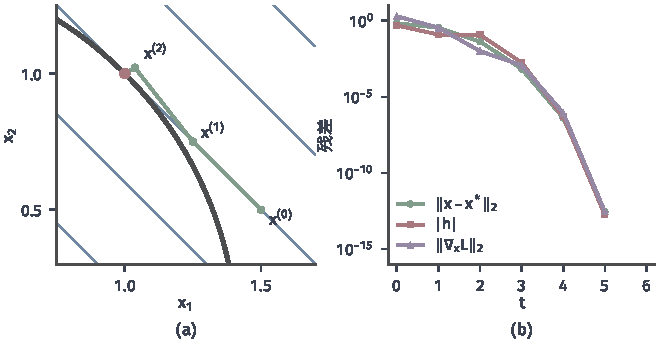
\includegraphics[width=112mm]{figures/05-optimization/06-constrained-optimization/matplotlib/sqp-newton-path/figure.pdf}
 \caption{问题~\eqref{eq:sqp-circle}上全步长SQP的运行结果。(a)~路径（绿），中间各点都不在圆上。(b)~到解的距离、约束残差和Lagrange梯度随迭代的变化，纵轴为对数，后几轮每步的有效数字大致翻倍。}
 \label{fig:sqp-newton-path}
\end{BookInlineFigure}

表中有两点值得注意。第一，约束残差的下降并不均匀，$t=1$到$t=2$几乎没有变化，因为这一步走得长，二阶误差$\lVert\bm{d}\rVert_2^2$把线性化的好处抵消了。第二，从$t=2$起误差大致平方下降，这是Newton型方法的标志，第~\ref{sec:sqp-convergence}节给出证明。

\section{有效集法（Active-Set）}
\label{sec:sqp-active-set}

等式QP一步就能解完。不等式的困难在于事先不知道解处哪些不等式取等号：如果知道，把它们当等式，其余的扔掉，就回到了上一节。接下来要弄清：怎样一边迭代、一边找出这些约束？

这就像按预算线分配资源。有些预算在最优方案中被用尽，是真正起作用的边界；有些还有富余，暂时可以当它不存在。麻烦在于，只有解出方案后才知道哪些用尽了。有效集法的做法是先猜一组，解一下，看哪里不对，再改这一组。这个类比的边界是，算法改的是它自己维护的集合，这个集合不必与当前点真实触碰的边界完全相同。

\paragraph{要解的QP}
本节讨论一个独立的QP，记号与局部模型无关，变量写作$\bm{x}$：
\begin{equation}
 \min_{\bm{x}\in\mathbb{R}^n}\ q(\bm{x})=\frac12\bm{x}^\top\bm{B}\bm{x}+\langle\bm{c},\bm{x}\rangle
 \quad\text{s.t.}\quad\langle\bm{a}_i,\bm{x}\rangle\leq b_i,\quad i=1,\ldots,m.
 \label{eq:sqp-as-qp}
\end{equation}
等式约束若有，始终留在下面要定义的集合里，写法上不必单列。全节的例子是平面上到点$\bm{c}^\circ=(4,2)^\top$的投影：
\begin{equation}
 \begin{gathered}
 q(\bm{x})=\frac12\lVert\bm{x}-\bm{c}^\circ\rVert_2^2,\\
 g_1:\ x_1+x_2\leq3,\quad g_2:\ -x_1\leq0,\quad g_3:\ -x_2\leq0,\quad g_4:\ x_1+2x_2\leq4.
 \end{gathered}
 \label{eq:sqp-as-example}
\end{equation}
它的$\bm{B}=\bm{I}$，$\bm{c}=-\bm{c}^\circ$，可行域是顶点为$(0,0),(3,0),(2,1),(0,2)$的四边形。

\paragraph{活动约束与工作集}
先把两个容易混淆的集合分开。在可行点$\bm{x}$处，取等号的约束构成\term{活动集}（active set），它由$\bm{x}$决定。算法还维护一个下标集合$\bm{W}$，这一轮把其中的约束当等式处理，它称为\term{工作集}（working set），由算法的历史决定。

可行点上工作集总是活动集的子集，但两者不必相等。图~\ref{fig:sqp-active-vs-working}给出三种情形：(a)~点贴着$g_3$的边，$g_3$活动，算法却可能没把它放进工作集；(b)~在顶点$(3,0)$处两条约束都活动，工作集可以只含其中一条；(c)~两者重合。到了解处，算法想要的是工作集恰好为那些乘子为正的约束。

\begin{BookInlineFigure}
 \centering
 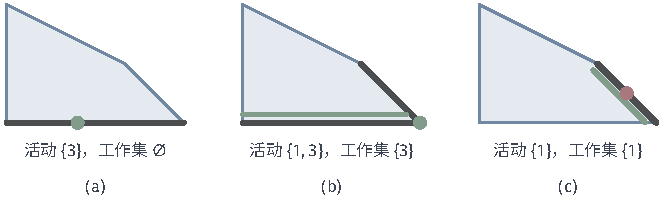
\includegraphics[width=112mm]{figures/05-optimization/06-constrained-optimization/tikz/sqp-active-vs-working/figure.pdf}
 \caption{活动集与工作集的区别，可行域取例~\eqref{eq:sqp-as-example}的四边形。深灰粗线是当前点真实触碰的边，绿色细带标出算法放进工作集的约束，圆点是当前点（红点为解）。}
 \label{fig:sqp-active-vs-working}
\end{BookInlineFigure}

\subsection{工作集的更新}
\label{sec:sqp-working-set}

本小节假设$\bm{B}\succ\bm{0}$，并且工作集中的约束梯度始终线性无关，已有一个可行的初始点。这样的初始点可以用第~\ref{chap:simplex-method}章两阶段法那样的辅助问题找到。

\paragraph{主要思想}
设$\bm{x}^{(t)}$可行，工作集为$\bm{W}$。把$\bm{W}$中的约束当等式，其余的先不管，问“从这里出发沿这张面能走到哪里”。写成对步$\bm{d}$的等式QP，并利用$\nabla q(\bm{x}^{(t)})=\bm{B}\bm{x}^{(t)}+\bm{c}$：
\begin{equation}
 \min_{\bm{d}}\ \frac12\bm{d}^\top\bm{B}\bm{d}+\langle\nabla q(\bm{x}^{(t)}),\bm{d}\rangle
 \quad\text{s.t.}\quad\langle\bm{a}_i,\bm{d}\rangle=0,\quad i\in\bm{W}.
 \label{eq:sqp-as-eqp}
\end{equation}
约束里右端是$0$，因为$\bm{W}$中的约束已经取等号，步不能破坏它们。结果分两种情况。

第一种，$\bm{d}\neq\bm{0}$。沿$\bm{d}$能降低$q$，但工作集以外的约束可能挡路。$\bm{W}$以外的约束$i$只在$\langle\bm{a}_i,\bm{d}\rangle>0$时才会变紧，走到边界所允许的比例是$(b_i-\langle\bm{a}_i,\bm{x}^{(t)}\rangle)/\langle\bm{a}_i,\bm{d}\rangle$。取其中最小的一个，并且不超过$1$，得到\term{比值检验}（ratio test）：
\begin{equation}
 \alpha^{(t)}=\min\Bigl\{1,\ \min_{i\notin\bm{W},\,\langle\bm{a}_i,\bm{d}\rangle>0}
 \frac{b_i-\langle\bm{a}_i,\bm{x}^{(t)}\rangle}{\langle\bm{a}_i,\bm{d}\rangle}\Bigr\}.
 \label{eq:sqp-ratio}
\end{equation}
新点是$\bm{x}^{(t)}$加上$\alpha^{(t)}\bm{d}$。若$\alpha^{(t)}<1$，取到最小值的约束称为\term{阻挡约束}（blocking constraint），把它加入工作集。它满足$\langle\bm{a}_b,\bm{d}\rangle>0$，而$\bm{W}$中的约束都有$\langle\bm{a}_i,\bm{d}\rangle=0$，所以它不在$\bm{W}$的约束梯度张成的子空间内，加入后仍线性无关。

第二种，$\bm{d}=\bm{0}$。当前点已是这张面上的最小点，该看乘子了。方程~\eqref{eq:sqp-kkt-system}的第一行此时给出
\begin{equation}
 \bm{B}\bm{x}^{(t)}+\bm{c}+\sum_{i\in\bm{W}}\lambda_i\bm{a}_i=\bm{0}.
 \label{eq:sqp-as-multiplier}
\end{equation}
若所有$\lambda_i\geq0$，再令$\bm{W}$以外的乘子为零，KKT条件全部成立，$\bm{B}\succ\bm{0}$时这就是全局最优解。

若有某个$\lambda_k<0$，负乘子说明这条约束不该被按住：它的影子价格是负的，相当于“放松这条预算，成本反而升高”，反过来说，向可行域内部离开这条边能让目标下降。下面的引理把这句话说准。

\begin{lemma}[释放负乘子约束]
\label{lem:sqp-drop}
设$\bm{d}=\bm{0}$时的乘子满足$\lambda_k<0$，令$\bm{W}'=\bm{W}\setminus\{k\}$，并设$\bm{d}'$是把$\bm{W}$换成$\bm{W}'$后问题~\eqref{eq:sqp-as-eqp}的解。则$\bm{d}'\neq\bm{0}$，$\bm{d}'$严格降低$q$的模型，并且
\begin{equation}
 \langle\bm{a}_k,\bm{d}'\rangle<0.
 \label{eq:sqp-drop-direction}
\end{equation}
\end{lemma}

\begin{proof}
先证$\bm{d}'\neq\bm{0}$。若$\bm{d}'=\bm{0}$，则存在系数$\mu_i$使$\nabla q+\sum_{i\in\bm{W}'}\mu_i\bm{a}_i=\bm{0}$。把它与式~\eqref{eq:sqp-as-multiplier}相减，得到$\bm{W}$中约束梯度的一个线性关系，其中$\bm{a}_k$的系数是$\lambda_k\neq0$，与线性无关矛盾。

再看方向。$\bm{d}'$的驻定条件是
\[
 \bm{B}\bm{d}'+\nabla q+\sum_{i\in\bm{W}'}\mu_i\bm{a}_i=\bm{0}.
\]

把式~\eqref{eq:sqp-as-multiplier}中的$\nabla q$代入，得
\[
 \bm{B}\bm{d}'=\sum_{i\in\bm{W}'}(\lambda_i-\mu_i)\bm{a}_i+\lambda_k\bm{a}_k.
\]

用$(\bm{d}')^\top$左乘，并注意$i\in\bm{W}'$时$\langle\bm{a}_i,\bm{d}'\rangle=0$，得到
\[
 (\bm{d}')^\top\bm{B}\bm{d}'=\lambda_k\langle\bm{a}_k,\bm{d}'\rangle.
\]
左端为正，$\lambda_k<0$，所以式~\eqref{eq:sqp-drop-direction}成立。

最后，$\bm{d}'$是等式QP的最小点而$\bm{d}=\bm{0}$可行，且最小点唯一，所以模型值严格小于零，即严格小于$\bm{d}=\bm{0}$时的模型值。
\end{proof}

式~\eqref{eq:sqp-drop-direction}的含义是，走$\bm{d}'$时被释放的约束$k$严格变松，点确实离开了这条边，不会立刻违反它。图~\ref{fig:sqp-activeset-multiplier}是例子中的这两个时刻。

\begin{BookInlineFigure}
 \centering
 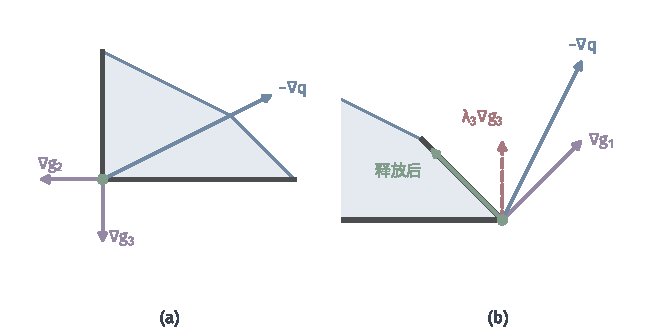
\includegraphics[width=112mm]{figures/05-optimization/06-constrained-optimization/matplotlib/sqp-activeset-multiplier/figure.pdf}
 \caption{乘子的符号。蓝色箭头是$-\nabla q$，紫色箭头是工作集约束的梯度，深灰粗线是工作集对应的边。(a)~原点处$-\nabla q=(4,2)^\top$指向可行域内部，它分解到两个向外的梯度上时系数都是负的。(b)~顶点$(3,0)^\top$处，$-\nabla q=\nabla g_1+\lambda_3\nabla g_3$，其中$\lambda_1=1$，$\lambda_3=-1$；红色虚线箭头是$\lambda_3\nabla g_3$。释放$g_3$后沿$g_1$的边（绿）走。}
 \label{fig:sqp-activeset-multiplier}
\end{BookInlineFigure}

整个逻辑可以画成图~\ref{fig:sqp-activeset-flow}。每一轮只改动工作集中的一条约束，或者加入一条，或者释放一条。

\begin{BookInlineFigure}
 \centering
 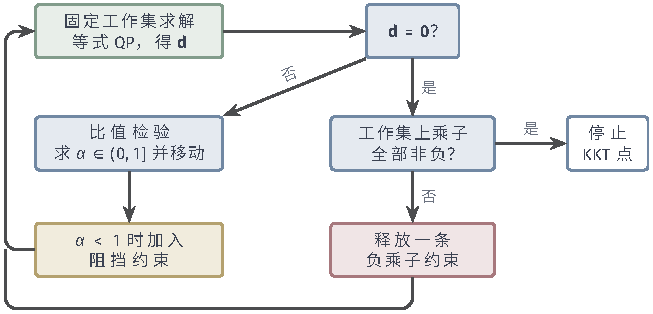
\includegraphics[width=112mm]{figures/05-optimization/06-constrained-optimization/tikz/sqp-activeset-flow/figure.pdf}
 \caption{有效集法一轮的判断。先求步；步非零则做比值检验，受阻时加入一条约束；步为零则看乘子，全部非负时停止，否则释放一条负乘子约束。}
 \label{fig:sqp-activeset-flow}
\end{BookInlineFigure}

\needspace{6\baselineskip}
\paragraph{变量}
\begin{itemize}
 \item $\bm{x}^{(t)}\in\mathbb{R}^n$：当前可行点。
 \item $\bm{W}$：工作集，下标集合，其大小不超过$n$。
 \item $\bm{A}_{\bm{W}}$：以$\bm{a}_i^\top$（$i\in\bm{W}$）为行的矩阵；$\bm{Z}_{\bm{W}}$：其零空间的基。
 \item $\bm{d}^{(t)}\in\mathbb{R}^n$：等式QP的解；$\lambda_i$（$i\in\bm{W}$）：工作集上的乘子。
\end{itemize}

\paragraph{初始化}
取可行点$\bm{x}^{(0)}$和一个工作集$\bm{W}$，其约束在$\bm{x}^{(0)}$处活动且梯度线性无关。例中取原点和它处的两条活动约束：
\[
 \bm{x}^{(0)}=(0,0)^\top,\qquad\bm{W}=\{2,3\}.
\]
目标值是$q(\bm{x}^{(0)})=10$。

\needspace{6\baselineskip}
\paragraph{每轮更新}
\begin{enumerate}
 \item 求步。由式~\eqref{eq:sqp-reduced-step}，取$\bm{h}=\bm{0}$，等式QP的解是
 \begin{equation}
  \bm{d}^{(t)}=-\bm{Z}_{\bm{W}}\bigl(\bm{Z}_{\bm{W}}^\top\bm{B}\bm{Z}_{\bm{W}}\bigr)^{-1}\bm{Z}_{\bm{W}}^\top\bigl(\bm{B}\bm{x}^{(t)}+\bm{c}\bigr).
  \label{eq:sqp-as-step}
 \end{equation}
 例中第一轮$\bm{W}=\{2,3\}$，零空间只有零向量，$\bm{d}^{(0)}=\bm{0}$。

 \item 若$\bm{d}^{(t)}=\bm{0}$，由式~\eqref{eq:sqp-as-multiplier}解出$\lambda_i$。行满秩时，用$\bm{A}_{\bm{W}}$左乘即得
 \begin{equation}
  \bm{\lambda}_{\bm{W}}=-\bigl(\bm{A}_{\bm{W}}\bm{A}_{\bm{W}}^\top\bigr)^{-1}\bm{A}_{\bm{W}}\bigl(\bm{B}\bm{x}^{(t)}+\bm{c}\bigr).
  \label{eq:sqp-as-lambda}
 \end{equation}
 全部非负就停止；否则从$\bm{W}$中去掉乘子最小的约束，令$\bm{x}^{(t+1)}=\bm{x}^{(t)}$，进入下一轮。

 例中第一轮$\nabla q=(-4,-2)^\top$，方程~\eqref{eq:sqp-as-multiplier}给出$\lambda_2=-4$，$\lambda_3=-2$。两个都是负的，释放$g_2$，得$\bm{W}=\{3\}$，$\bm{x}^{(1)}=\bm{x}^{(0)}$。

 \item 若$\bm{d}^{(t)}\neq\bm{0}$，由式~\eqref{eq:sqp-ratio}算$\alpha^{(t)}$，并移动到
 \begin{equation}
  \bm{x}^{(t+1)}=\bm{x}^{(t)}+\alpha^{(t)}\bm{d}^{(t)}.
  \label{eq:sqp-as-move}
 \end{equation}
 若$\alpha^{(t)}<1$，把阻挡约束加入$\bm{W}$。

 例中第二轮$\bm{W}=\{3\}$，$\bm{Z}_{\bm{W}}=(1,0)^\top$，由式~\eqref{eq:sqp-as-step}得$\bm{d}^{(1)}=(4,0)^\top$。比值检验只看$\langle\bm{a}_i,\bm{d}\rangle>0$的$g_1$和$g_4$：
 \[
  g_1:\ \frac{3}{4}=0.75,\qquad g_4:\ \frac{4}{4}=1.
 \]
 于是$\alpha^{(1)}=0.75$，受阻于$g_1$，得
 \[
  \bm{x}^{(2)}=(3,0)^\top,\qquad\bm{W}=\{1,3\},\qquad q(\bm{x}^{(2)})=2.5.
 \]

 第三轮零空间又只有零向量，$\bm{d}^{(2)}=\bm{0}$。此时$\nabla q=(-1,-2)^\top$，乘子满足
 \[
  \begin{bmatrix}-1\\-2\end{bmatrix}+\lambda_1\begin{bmatrix}1\\1\end{bmatrix}+\lambda_3\begin{bmatrix}0\\-1\end{bmatrix}=\bm{0}.
 \]
 第一行给$\lambda_1=1$，第二行给$\lambda_3=-1$。释放$g_3$，得$\bm{W}=\{1\}$，$\bm{x}^{(3)}=\bm{x}^{(2)}$。

 第四轮$\bm{Z}_{\bm{W}}=(1,-1)^\top$，$\bm{Z}_{\bm{W}}^\top\bm{Z}_{\bm{W}}=2$，$\bm{Z}_{\bm{W}}^\top\nabla q=1$。由式~\eqref{eq:sqp-as-step}，
 \[
  \bm{d}^{(3)}=-\frac12\begin{bmatrix}1\\-1\end{bmatrix}=(-0.5,\ 0.5)^\top.
 \]
 比值检验中$g_2$的比值是$3/0.5=6$，$g_4$的比值是$1/0.5=2$，都大于$1$，所以走满一步：
 \[
  \bm{x}^{(4)}=(2.5,\ 0.5)^\top,\qquad q(\bm{x}^{(4)})=2.25.
 \]

 \item 重复第1至3步，直到第2步发现乘子全部非负。

 例中第五轮$\bm{W}=\{1\}$，此时$\nabla q=(-1.5,-1.5)^\top$与$\bm{Z}_{\bm{W}}$正交，所以这一轮的步为零。乘子由下式确定：
 \[
  \nabla q+\lambda_1(1,1)^\top=\bm{0},\qquad\lambda_1=1.5\geq0.
 \]
 乘子非负，停止。
\end{enumerate}

最终得到$\bm{x}^\star=(2.5,0.5)^\top$，$g_1$是唯一的活动约束，影子价格$\lambda_1=1.5$。路径如图~\ref{fig:sqp-activeset-path}，每个停留的点上都发生一次工作集的变动。

\begin{BookInlineFigure}
 \centering
 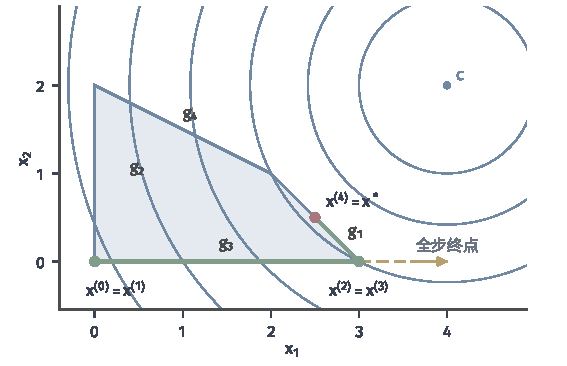
\includegraphics[width=96mm]{figures/05-optimization/06-constrained-optimization/matplotlib/sqp-activeset-path/figure.pdf}
 \caption{例~\eqref{eq:sqp-as-example}上有效集法的路径（绿）。浅蓝区域是可行域，蓝色同心圆是$q$的等高线，蓝点是无约束最小点$\bm{c}^\circ$。沿$g_3$的边本想走到$(4,0)^\top$（黄色虚线），在$(3,0)^\top$被$g_1$挡住；释放$g_3$后沿$g_1$走到红点，算法结束。}
 \label{fig:sqp-activeset-path}
\end{BookInlineFigure}

\paragraph{为什么有限步结束}
工作集的取法只有有限多种，只要同一个工作集不会被重复“解完”，算法就会停。

\begin{theorem}[有效集法的有限终止]
\label{thm:sqp-as-finite}
设$\bm{B}\succ\bm{0}$，工作集中的约束梯度始终线性无关，并且每个$\bm{d}^{(t)}\neq\bm{0}$的轮次都有$\alpha^{(t)}>0$。则算法在有限轮后停在问题~\eqref{eq:sqp-as-qp}的全局最优解。
\end{theorem}

\begin{proof}
称$\bm{d}^{(t)}=\bm{0}$的轮次为到站。两次到站之间，$\bm{W}$只增不减，所以至多有$n$轮比值检验，否则$\bm{W}$的大小超过$n$，与线性无关矛盾。由此到站必然反复发生或算法停止。

下面说明工作集不会在两次到站时重复。到站时$\bm{x}^{(t)}$是$q$在工作集约束所定义的仿射面上的唯一最小点，所以到站时的目标值由$\bm{W}$决定。

由引理~\ref{lem:sqp-drop}，到站后释放一条约束得到的步非零，严格降低模型。凸二次函数沿下降方向走$\alpha\in(0,1]$仍严格下降，而假设保证$\alpha>0$。所以相邻两次到站的目标值严格递减，同一个$\bm{W}$不会出现两次。工作集的个数有限，算法必在有限轮后到站且乘子全部非负，此时KKT条件成立，由凸性得全局最优。
\end{proof}

定理要求每次移动的步长为正。这个条件失效时会发生什么，是下面要讨论的。

\paragraph{退化、平局与热启动}
假设例中$g_4$改成$x_1+2x_2\leq3$。第二轮的比值检验中，$g_1$和$g_4$的比值都是$0.75$，出现平局，只能加入一条，另一条在下一点也活动却不在工作集中。

这一点已经是退化的：图~\ref{fig:sqp-degenerate}(b)那样，过一点的活动约束多于$n$条或梯度线性相关。这时比值检验可能算出$\alpha^{(t)}=0$，点不动，只有工作集换了一条。一连串这样的零步有可能转回原来的工作集，形成循环，定理的条件也就破坏了。

\begin{BookInlineFigure}
 \centering
 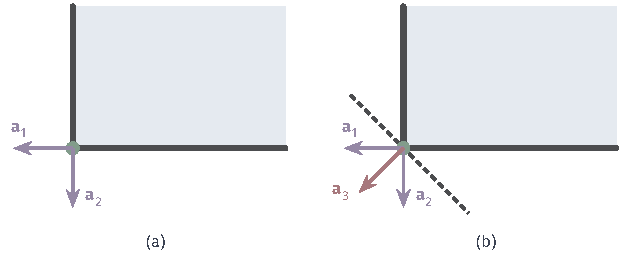
\includegraphics[width=100mm]{figures/05-optimization/06-constrained-optimization/tikz/sqp-degenerate/figure.pdf}
 \caption{顶点处的约束梯度。(a)~两条活动约束，紫色梯度线性无关，工作集的选取没有歧义。(b)~第三条约束（虚线）也经过同一点，三个梯度在平面内线性相关，工作集只能放下其中两条，走零步时点不动而工作集在变。}
 \label{fig:sqp-degenerate}
\end{BookInlineFigure}

实用的防范办法有两类。一类是确定性的选取规则，例如第~\ref{chap:simplex-method}章的Bland规则，在平局和释放时都按下标的固定顺序挑选，避免转圈。另一类是给约束右端加很小的扰动，让重合的边界分开，结束后再回到原数据上核对。释放时取最负的乘子是常用的选择，但它本身不防止循环。

有效集法还有一个明显的长处。如果手里有一个接近解的工作集，从它开始往往几轮就结束，这叫\term{热启动}（warm start）。SQP相邻两轮的QP数据只有微小变化，上一轮的工作集正是下一轮的好起点。内点法从内部出发，较难利用这种信息。每轮工作集只变一条约束，$\bm{K}$或$\bm{Z}$的分解也可以用低秩修正更新，不必重新分解。

\subsection{有效集法与SQP}
\label{sec:sqp-active-set-sqp}

把有效集法用在局部QP~\eqref{eq:sqp-qp}上时，变量是$\bm{d}$，$\bm{a}_i=\nabla g_i^{(t)}$，$b_i=-g_i^{(t)}$。本小节要回答的问题是：这样得到的工作集，和原问题解处真正活动的约束是什么关系？

\paragraph{工作集属于当前的线性化QP}
先看一个带不等式的例子，把问题~\eqref{eq:sqp-circle}的约束放宽，再加两条线性约束：
\begin{equation}
 \begin{gathered}
 \min_{\bm{x}}\ -x_1-x_2\\
 \text{s.t.}\quad g_1=x_1^2+x_2^2-2\leq0,\quad g_2=x_2-1.2\leq0,\quad g_3=-x_1\leq0.
 \end{gathered}
 \label{eq:sqp-ineq-example}
\end{equation}
解仍是$(1,1)^\top$，只有$g_1$活动，乘子$\lambda_1^\star=1/2$。下面用精确的Lagrange Hessian和全步长，从$\bm{x}^{(0)}=(0.5,1.7)^\top$、$\bm{\lambda}^{(0)}=(1,0,0)^\top$出发。

第一轮$\bm{B}^{(0)}=2\lambda_1^{(0)}\bm{I}=2\bm{I}$，约束的值和线性化约束是
\[
 \begin{gathered}
 g_1=1.14,\qquad g_2=0.5,\qquad g_3=-0.5,\\
 1.14+d_1+3.4\,d_2\leq0,\qquad 0.5+d_2\leq0,\qquad -0.5-d_1\leq0.
 \end{gathered}
\]

模型的目标是$-d_1-d_2+d_1^2+d_2^2$。先试工作集$\{2\}$：取$d_2=-0.5$，$d_1$的最优值是$0.5$。检验其余约束，线性化的$g_1$值是
\[
 1.14+0.5+3.4\times(-0.5)=-0.06\leq0,
\]
线性化的$g_3$值是$-1\leq0$，都满足。乘子由第二个驻定方程$-1+2d_2+\hat\lambda_2=0$得$\hat\lambda_2=2\geq0$。所以QP的解是
\[
 \bm{d}^{(0)}=(0.5,\ -0.5)^\top,\qquad\hat{\bm{\lambda}}=(0,\ 2,\ 0)^\top,\qquad\bm{x}^{(1)}=(1,\ 1.2)^\top.
\]

这一步说明了两件事。其一，这一轮的工作集是$\{2\}$，而原问题解处活动的是$\{1\}$：工作集属于这一轮的线性化QP，不是对原问题的最终判断。其二，$\bm{d}^{(0)}$满足全部线性化约束，新点却有
\[
 g_1(\bm{x}^{(1)})=1+1.44-2=0.44>0.
\]
QP可行不代表原问题可行，图~\ref{fig:sqp-qp-vs-nonlinear}(a)画的就是这个缺口：步落在线性化的半平面内，却冲出了圆。

\begin{BookInlineFigure}
 \centering
 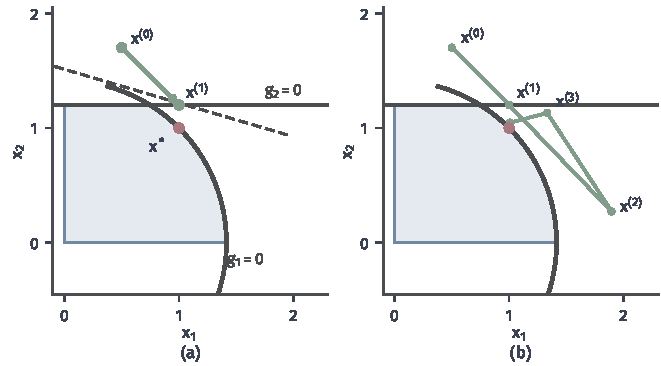
\includegraphics[width=112mm]{figures/05-optimization/06-constrained-optimization/matplotlib/sqp-qp-vs-nonlinear/figure.pdf}
 \caption{问题~\eqref{eq:sqp-ineq-example}上的SQP。浅蓝区域是真实可行域，深灰粗线是$g_1,g_2$的边界，绿色折线是迭代路径，红点是解。(a)~第一步，虚线是$g_1$在$\bm{x}^{(0)}$的线性化边界，$\bm{x}^{(1)}$满足线性化约束但在圆外。(b)~前五步的路径：工作集先后是$\{2\}$与$\{1\}$，迭代点在前几轮都不可行。}
 \label{fig:sqp-qp-vs-nonlinear}
\end{BookInlineFigure}

第二轮的乘子估计是$\lambda_1^{(1)}=0$，于是$\nabla^2_{\bm{x}\bm{x}}\mathcal{L}=\bm{0}$，子问题退化成线性规划。为了让子问题仍有曲率，这里临时取$\bm{B}^{(1)}=0.1\,\bm{I}$，这类修正下一节专门讨论。此后QP选中的工作集稳定为$\{1\}$，乘子很快接近$1/2$。图~\ref{fig:sqp-working-set-chart}列出各轮约束值和工作集。

\begin{BookInlineFigure}
 \centering
 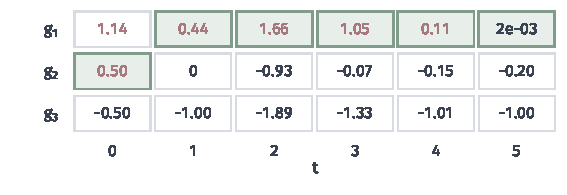
\includegraphics[width=96mm]{figures/05-optimization/06-constrained-optimization/matplotlib/sqp-working-set-chart/figure.pdf}
 \caption{问题~\eqref{eq:sqp-ineq-example}各轮的约束值$g_i(\bm{x}^{(t)})$，正值（红字）表示违反原约束，绿色格表示该约束在这一轮QP的最优工作集中。第一轮之后工作集稳定为$\{1\}$，而$g_1$的违反量要到后几轮才降下来。}
 \label{fig:sqp-working-set-chart}
\end{BookInlineFigure}

\paragraph{什么时候能认出解处的活动集}
图~\ref{fig:sqp-working-set-chart}的现象并不偶然。在解附近，QP的最优工作集会固定下来，且正好是原问题的活动集，此后的SQP就成了只含等式的SQP，上一节的结论都可以用。先复述第~\ref{chap:constrained-optimality}章的三个条件。设$(\bm{x}^\star,\bm{\lambda}^\star,\bm{\nu}^\star)$是KKT点，$\bm{S}^\star$是$\bm{x}^\star$处活动的不等式下标集。

\begin{itemize}
 \item 约束资格（LICQ）：活动不等式和全部等式的梯度在$\bm{x}^\star$处线性无关。
 \item 严格互补：对每个$i\in\bm{S}^\star$，有$\lambda_i^\star>0$。
 \item 二阶充分条件：$\nabla^2_{\bm{x}\bm{x}}\mathcal{L}$在解处沿活动约束梯度的零空间正定。在严格互补下，这就是该章临界锥上的二阶条件。
\end{itemize}

\begin{theorem}[解附近的活动集识别]
\label{thm:sqp-identification}
设上述三个条件成立。对任意有界的对称矩阵族$\{\bm{B}\}$，若它们在活动约束零空间上的约化矩阵一致正定，则存在$(\bm{x}^\star,\bm{\lambda}^\star,\bm{\nu}^\star)$的邻域，使得当当前点与乘子都在此邻域内时，QP~\eqref{eq:sqp-qp}有一个靠近$\bm{0}$的严格局部解$\bm{d}$，其活动集恰为$\bm{S}^\star$，乘子靠近$(\bm{\lambda}^\star,\bm{\nu}^\star)$。
\end{theorem}

\begin{proof}
把$\bm{S}^\star$中的不等式和全部等式都当作等式，写出方程~\eqref{eq:sqp-kkt-system}，其解记为$(\bm{d},\hat{\bm{\lambda}}_{\bm{S}^\star},\hat{\bm{\nu}})$，并令$\bm{S}^\star$以外的乘子为零。

由LICQ和约化矩阵的一致正定，KKT矩阵在该邻域内一致可逆（定理~\ref{thm:sqp-eqp}的论证与连续性）。在$(\bm{x}^\star,\bm{\lambda}^\star,\bm{\nu}^\star)$处方程右端使解为$\bm{d}=\bm{0}$，乘子为$(\bm{\lambda}^\star_{\bm{S}^\star},\bm{\nu}^\star)$。方程右端连续，而$\bm{B}\bm{d}$随$\bm{d}\to\bm{0}$趋于零，所以邻域足够小时$\bm{d}$靠近$\bm{0}$，乘子靠近其真值。

现在逐条核对条件~\eqref{eq:sqp-qp-kkt}。严格互补使$\hat\lambda_i>0$（$i\in\bm{S}^\star$），乘子符号成立。对$i\notin\bm{S}^\star$，有$g_i(\bm{x}^\star)<0$，由连续性$g_i+\langle\nabla g_i,\bm{d}\rangle<0$，这些约束严格满足。所以$\bm{d}$是QP的KKT点，活动集恰为$\bm{S}^\star$。

最后，活动约束的乘子严格为正，且$\bm{B}$在其零空间上正定，所以二阶充分条件对这个QP成立，$\bm{d}$是严格局部解。
\end{proof}

这个定理只断言“存在这样一个解”。QP非凸时可能还有别的局部解，求解器未必返回这一个；若从上一轮的工作集热启动，实际中通常就落在这一个上。条件各有其用：缺少严格互补时，$\lambda_i^\star=0$的约束可能在相邻两轮时进时出；缺少约束资格时乘子不唯一，方程组可能接近奇异。

\paragraph{原问题的检查不能省}
工作集稳定是解附近的现象，远离解时它可能频繁变动。即使稳定了，QP可行也只是切平面上的可行。所以有效集法解完子问题后，仍然要回到原问题检验新点的目标和约束，这正是第~\ref{sec:sqp-acceptance}节的内容。

\section{曲率的处理}
\label{sec:sqp-curvature}

式~\eqref{eq:sqp-lagrangian-hessian}的矩阵在解附近很好，远离解时却可能不定。这就需要回答：$\bm{B}^{(t)}$既要反映真实的局部曲率，又要让子问题有意义、让步能被接受，这两者怎样兼顾？

\paragraph{KKT系统可解不等于模型是碗}
先把两件容易混淆的事分开。设只有一条约束$d_2=0$，即$\bm{A}=(0,1)$，线性项$\bm{c}=(-0.6,0.3)^\top$，比较三个矩阵：
\[
 \bm{B}_a=\begin{bmatrix}1&0\\0&1\end{bmatrix},\qquad
 \bm{B}_b=\begin{bmatrix}1&0\\0&-1\end{bmatrix},\qquad
 \bm{B}_c=\begin{bmatrix}-1&0\\0&1\end{bmatrix}.
\]

这里零空间由$\bm{e}_1$张成，约化Hessian就是左上角的元素。三种情形下KKT矩阵都可逆，解都由$B_{1,1}d_1=0.6$给出，对应的$\bm{d}$分别是
\[
 (0.6,\ 0)^\top,\qquad(0.6,\ 0)^\top,\qquad(-0.6,\ 0)^\top.
\]

图~\ref{fig:sqp-kkt-vs-convexity}是这三个模型。情形(a)是凸的，解是最小点。情形(b)的$\bm{B}$不定，整个二次目标不是凸的，可是沿约束直线它向上弯，解仍是约束上的最小点。情形(c)的$\bm{B}$同样不定，沿直线却向下弯，解是约束上的最大点，模型沿直线无下界。

\begin{BookInlineFigure}
 \centering
 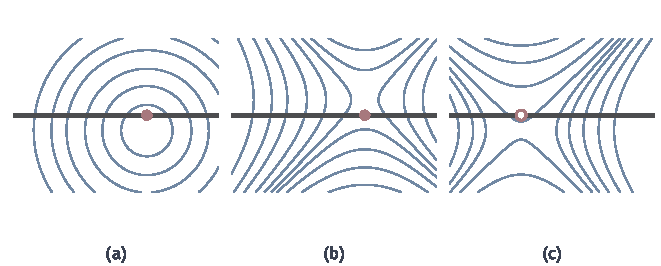
\includegraphics[width=112mm]{figures/05-optimization/06-constrained-optimization/matplotlib/sqp-kkt-vs-convexity/figure.pdf}
 \caption{三个KKT矩阵都可逆的模型，蓝线是二次目标的等高线，深灰粗线是约束$d_2=0$。(a)~$\bm{B}$正定，解（红点）是最小点。(b)~$\bm{B}$不定而约化Hessian为正，解仍是约束上的最小点。(c)~约化Hessian为负，KKT系统的解（空心点）是约束上的最大点。}
 \label{fig:sqp-kkt-vs-convexity}
\end{BookInlineFigure}

所以有三个不同的判断：KKT矩阵可逆；约化Hessian正定；$\bm{B}$在全空间正定。第三个推出第二个，第二个在行满秩时推出第一个，反过来都不成立。整个二次目标凸不凸，本身不是SQP需要的条件。

这几件事可以通过分解读出来。矩阵的\term{惯性}（inertia）是其正、负、零特征值的个数。$\bm{A}$行满秩时可以证明，$\bm{K}$的惯性等于$\bm{Z}^\top\bm{B}\bm{Z}$的惯性再各加上$p$个正、负特征值，证明要用一次合同变换，篇幅不长，读者可查阅专著\scite{math-nocedal2006numerical}。因此约化Hessian正定当且仅当$\bm{K}$恰有$n$个正特征值和$p$个负特征值。

用上面三个矩阵核对。这里$n=2$，$p=1$，$\bm{K}_a$和$\bm{K}_b$的惯性都是$(2,1,0)$；$\bm{K}_c$的特征值是$-1$和$(1\pm\sqrt5)/2$，惯性是$(1,2,0)$，多出一个负特征值，正好标记了错误的曲率。

子问题由什么方法求解，决定了实际要满足什么。表~\ref{tab:sqp-curvature-needs}按求解器列出要求。

\begin{BookInlineTable}
 \centering
 \begin{tabular}{ll}
  \toprule
  子问题的解法 & 对$\bm{B}$的实际要求\\
  \midrule
  直接解KKT系统 & 可逆即可解，是否最小点要另查惯性\\
  零空间方法 & 约化Hessian正定\\
  有效集法 & 每个工作集的约化Hessian正定\\
  要求凸QP的内点法等 & 通常要求$\bm{B}$半正定\\
  \bottomrule
 \end{tabular}
 \caption{不同子问题解法对曲率的要求。}
 \label{tab:sqp-curvature-needs}
\end{BookInlineTable}

\subsection{Hessian修正}
\label{sec:sqp-hessian-modification}

\paragraph{负曲率的例子}
乘子估计差得远时，精确的$\bm{B}$就可能是错的。回到问题~\eqref{eq:sqp-circle}的$\bm{x}^{(0)}=(1.5,0.5)^\top$，把乘子估计错成$\nu=-1$，于是$\bm{B}=2\nu\bm{I}=-2\bm{I}$，在任何方向上都向下弯。

KKT系统依然可解。第一行是$-2\bm{d}+\bm{g}+\hat\nu\bm{A}^\top=\bm{0}$，由此
\[
 \bm{d}=\frac12\bigl(\bm{g}+\hat\nu\bm{A}^\top\bigr)=\frac12\begin{bmatrix}3\hat\nu-1\\\hat\nu-1\end{bmatrix}.
\]

代入第二行$\bm{A}\bm{d}=-0.5$，左端是$5\hat\nu-2$，于是
\[
 \hat\nu=0.3,\qquad\bm{d}=(-0.05,\ -0.35)^\top.
\]

这个步是否合用，要沿线性化约束看模型。把允许的步写成$\bm{d}=\bm{d}_Y+s\bm{t}$，其中$\bm{d}_Y=(-0.15,-0.05)^\top$是第~\ref{sec:sqp-equality-qp}节的法向段，$\bm{t}=(-1,3)^\top/\sqrt{10}$是虚线的单位方向。代入模型并利用$\bm{d}_Y\perp\bm{t}$，得到
\[
 q(s)=0.175-0.632\,s-s^2.
\]

上式对$s$向下弯，模型沿线性化约束没有下界。KKT系统给出的$\bm{d}$对应$s\approx-0.316$，正是图~\ref{fig:sqp-curvature-repair}红线的最高点。求解这个方程得到的是模型的最大点，把它当作下降步是错的。

\begin{BookInlineFigure}
 \centering
 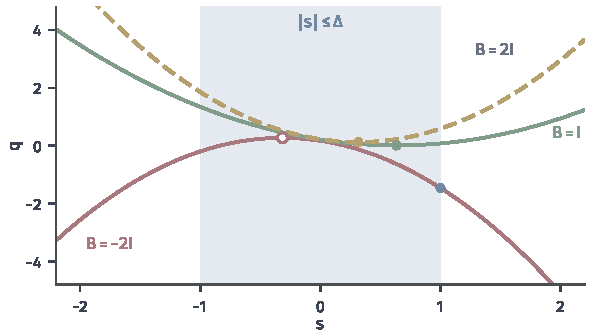
\includegraphics[width=100mm]{figures/05-optimization/06-constrained-optimization/matplotlib/sqp-curvature-repair/figure.pdf}
 \caption{沿线性化约束的模型$q(s)$，$s$是沿虚线方向的位移。红线是$\bm{B}=-2\bm{I}$，空心点是KKT系统的解，它是最大点。绿线、黄色虚线是移位后的$\bm{B}=\bm{I}$与$\bm{B}=2\bm{I}$，圆点是各自的最小点。浅蓝带是信赖域$\lvert s\rvert\leq\Delta=1$，蓝点是原模型在带内的最小点。}
 \label{fig:sqp-curvature-repair}
\end{BookInlineFigure}

\paragraph{先核对模型是否无界}
含不等式时情况稍有不同。不等式可能把下降方向挡住，QP于是有解，可是解落在边界上，是负曲率推过去的，未必是好步。所以出现负曲率时要回答两个问题：子问题本身有没有下界，以及当前这个步是否适合接受。处理的办法有三类，它们改变的东西不同。

\paragraph{移位}
第一种办法是把$\bm{B}$换成$\bm{B}+\tau\bm{I}$，这是第~\ref{chap:second-order-methods}章修正Newton法的直接推广。取$\tau$从小到大试，每次分解后检查惯性，直到约化Hessian正定。例中约化Hessian是$-2$，需要$\tau>2$。

取$\tau=3$，就是$\bm{B}=\bm{I}$。解KKT系统，第一行给$\bm{d}=(1-3\hat\nu,1-\hat\nu)^\top$，第二行给$4-10\hat\nu=-0.5$，于是
\[
 \hat\nu=0.45,\qquad\bm{d}=(-0.35,\ 0.55)^\top.
\]

移位改的是模型本身，而且改的是所有方向的曲率。$\tau$越大，步越短、越偏向梯度方向。例中$\tau=4$时步变成$(-0.25,0.25)^\top$，图~\ref{fig:sqp-curvature-repair}的黄线最低点比绿线更靠近$s=0$，就是这个效果。

\paragraph{约化曲率修正}
第二种办法只动约化Hessian。在式~\eqref{eq:sqp-reduced-step}中，把$\bm{Z}^\top\bm{B}\bm{Z}$换成一个正定矩阵，比如把负特征值取绝对值，其他量不变。例中用$\lvert-2\rvert=2$，右端不变，得到
\[
 s=\frac{0.632}{2}=0.316,\qquad\bm{d}=(-0.25,\ 0.25)^\top.
\]

这里结果恰好和$\tau=4$相同，因为$\bm{d}_Y$与$\bm{t}$正交，$\bm{B}$又是单位阵的倍数。一般两者不同：约化修正不改变法向段，也保留了$\bm{B}$在约束法方向上的信息。

\paragraph{信赖域限制}
第三种办法不改模型，而是限制步能走多远，这是第~\ref{chap:trust-region}章的想法。例中加$\lvert s\rvert\leq\Delta=1$，模型在带内的最小点在边界$s=1$，那里的模型值是$-1.457$，另一端$s=-1$的模型值是$-0.193$。

信赖域的好处是负曲率不用消除，它甚至被用来走得更远。约束优化中要多注意一件事：线性化约束和信赖域可能相互矛盾，它们的交集可能是空的。常见的处理是先取法向段，要求它只占信赖域的一部分，再在剩下的范围内取切向段。

\begin{BookInlineTable}
 \centering
 \begin{tabular}{lll}
  \toprule
  做法 & 改变了什么 & 代价或风险\\
  \midrule
  移位$\bm{B}+\tau\bm{I}$ & 所有方向的曲率 & 反复分解，步偏向梯度\\
  约化曲率修正 & 零空间内的曲率 & 需要显式的$\bm{Z}$\\
  信赖域 & 允许的步长范围 & 约束可能不相容\\
  \bottomrule
 \end{tabular}
 \caption{处理负曲率的三类办法。}
 \label{tab:sqp-modification}
\end{BookInlineTable}

这些办法各自改变了模型或步长范围。一个可解的KKT系统本身不能保证解是极小步，判断的依据只能是约化曲率或惯性。修正后的步还要经过第~\ref{sec:sqp-acceptance}节的检验。

\subsection{拟Newton近似}
\label{sec:sqp-quasi-newton}

精确的式~\eqref{eq:sqp-lagrangian-hessian}要求所有$m+p+1$个函数的二阶导数，这常常是SQP最贵也最难编写的一部分。第~\ref{chap:quasi-newton}章的办法是从梯度之差积累曲率。本小节要解决的问题是：在约束问题上，这个差该怎么取，又该怎样保持近似矩阵可用？

\paragraph{割线信息}
要近似的是Lagrange函数对$\bm{x}$的Hessian，所以差分的对象是Lagrange梯度。两点必须用同一组乘子，否则差分中混入乘子的变化，就不再是对$\nabla^2_{\bm{x}\bm{x}}\mathcal{L}$的测量。取新的乘子估计，令
\begin{equation}
 \begin{aligned}
 \bm{s}^{(t)}&=\bm{x}^{(t+1)}-\bm{x}^{(t)},\\
 \bm{y}^{(t)}&=\nabla_{\bm{x}}\mathcal{L}(\bm{x}^{(t+1)},\bm{\lambda}^{(t+1)},\bm{\nu}^{(t+1)})
 -\nabla_{\bm{x}}\mathcal{L}(\bm{x}^{(t)},\bm{\lambda}^{(t+1)},\bm{\nu}^{(t+1)}).
 \end{aligned}
 \label{eq:sqp-secant-pair}
\end{equation}

BFGS更新的公式与第~\ref{chap:quasi-newton}章相同，这里省去上标，新矩阵记作$\bm{B}^{+}$：
\begin{equation}
 \bm{B}^{+}=\bm{B}-\frac{\bm{B}\bm{s}\bm{s}^\top\bm{B}}{\bm{s}^\top\bm{B}\bm{s}}+\frac{\bm{y}\bm{y}^\top}{\bm{s}^\top\bm{y}}.
 \label{eq:sqp-bfgs}
\end{equation}

例中取第一步$\bm{s}=(-0.25,0.25)^\top$，$\hat\nu=0.5$，初始矩阵$\bm{B}=2\bm{I}$。这时Lagrange梯度是$\bm{x}-(1,1)^\top$，由它在两点之差得到
\[
 \bm{y}=\bm{s}=(-0.25,\ 0.25)^\top,\qquad\bm{s}^\top\bm{y}=0.125,\qquad\bm{s}^\top\bm{B}\bm{s}=0.25.
\]

代入式~\eqref{eq:sqp-bfgs}，并用$\bm{B}\bm{s}=2\bm{s}$，修正项化成$\bm{s}\bm{s}^\top$的倍数：
\[
 \bm{B}^{+}=2\bm{I}-16\,\bm{s}\bm{s}^\top+8\,\bm{s}\bm{s}^\top
 =\begin{bmatrix}1.5&0.5\\0.5&1.5\end{bmatrix}.
\]

可以核对割线条件$\bm{B}^{+}\bm{s}=\bm{y}$：沿$\bm{s}$的曲率从$2$变成了真实的$1$，与$\bm{s}$正交的方向仍保持$2$，因为这一次测量对那个方向没有提供信息。

\paragraph{曲率条件与阻尼}
无约束时，Wolfe线搜索能保证$\bm{s}^\top\bm{y}>0$。约束问题却不同，$\nabla^2_{\bm{x}\bm{x}}\mathcal{L}$在解处也可能是不定的，这时走出来的$\bm{s}$可能真的带着负曲率，不能靠步长选取来排除。如果$\bm{s}^\top\bm{y}\leq0$，式~\eqref{eq:sqp-bfgs}会毁掉正定性。

\term{阻尼BFGS}（damped BFGS）把$\bm{y}$换成它和$\bm{B}\bm{s}$的一个组合$\bm{r}$，组合比例只在测量不够好时才起作用：
\begin{equation}
 \begin{gathered}
 \bm{r}=\theta\bm{y}+(1-\theta)\bm{B}\bm{s},\\
 \theta=\begin{cases}
 1, & \bm{s}^\top\bm{y}\geq0.2\,\bm{s}^\top\bm{B}\bm{s},\\
 \dfrac{0.8\,\bm{s}^\top\bm{B}\bm{s}}{\bm{s}^\top\bm{B}\bm{s}-\bm{s}^\top\bm{y}}, & \text{否则}.
 \end{cases}
 \end{gathered}
 \label{eq:sqp-damped}
\end{equation}
然后在式~\eqref{eq:sqp-bfgs}中用$\bm{r}$代替$\bm{y}$。

第二种情形的$\theta$恰好使$\bm{s}^\top\bm{r}=0.2\,\bm{s}^\top\bm{B}\bm{s}>0$。把$\theta$代入即可验证：
\[
 \bm{s}^\top\bm{r}=\bm{s}^\top\bm{B}\bm{s}+\theta\bigl(\bm{s}^\top\bm{y}-\bm{s}^\top\bm{B}\bm{s}\bigr)=\bm{s}^\top\bm{B}\bm{s}-0.8\,\bm{s}^\top\bm{B}\bm{s}.
\]

所以更新后的矩阵总保持正定。图~\ref{fig:sqp-damped-rule}按上例的$\bm{s}^\top\bm{B}\bm{s}=0.25$画出这条规则。设乘子为负，真实曲率是$-2$，即$\bm{y}=-2\bm{s}$，$\bm{s}^\top\bm{y}=-0.25$，于是
\[
 \theta=\frac{0.8\times0.25}{0.25+0.25}=0.4,\qquad\bm{r}=0.4\bm{s}.
\]

沿$\bm{s}$的曲率更新后是$0.05/0.125=0.4$，即$\bm{s}^\top\bm{r}$除以$\bm{s}^\top\bm{s}$。它既不是测量到的$-2$，也不是原来的$2$。阻尼的代价是割线条件不再成立，矩阵不再记录真实的负曲率。

\begin{BookInlineFigure}
 \centering
 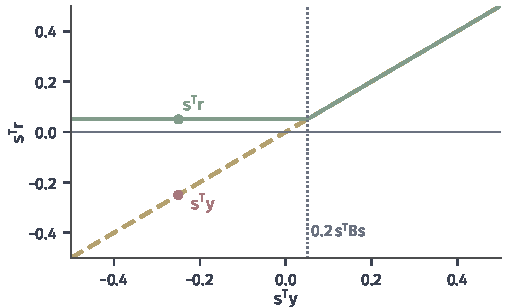
\includegraphics[width=86mm]{figures/05-optimization/06-constrained-optimization/matplotlib/sqp-damped-rule/figure.pdf}
 \caption{阻尼规则，$\bm{s}^\top\bm{B}\bm{s}=0.25$。黄色虚线是未加处理的$\bm{s}^\top\bm{y}$，绿线是阻尼后的$\bm{s}^\top\bm{r}$，它在虚线竖线以左被托在$0.2\,\bm{s}^\top\bm{B}\bm{s}=0.05$。红点是测量值$-0.25$，绿点是阻尼后的$0.05$。}
 \label{fig:sqp-damped-rule}
\end{BookInlineFigure}

\paragraph{成本与速度}
下面比较两种选择。精确Hessian每轮要算$m+p+1$个Hessian，但步是Newton型的，轮数少。拟Newton只需要梯度，却维护一个稠密的$n\times n$矩阵，破坏了$\bm{K}$可能具有的稀疏结构，这时可以改用有限记忆的表示。

图~\ref{fig:sqp-exact-bfgs-rate}是一个五变量问题上的比较，目标与约束为
\[
 \begin{gathered}
 f=\exp(x_1x_2x_3x_4x_5)-\tfrac12(x_1^3+x_2^3+1)^2,\\
 h_1=\lVert\bm{x}\rVert_2^2-10,\quad h_2=x_2x_3-5x_4x_5,\quad h_3=x_1^3+x_2^3+1.
 \end{gathered}
\]
从$(-1.8,1.7,1.9,-0.8,-0.8)^\top$与最小二乘乘子出发，精确Hessian的全步法$4$轮将误差降到$10^{-11}$以下；阻尼BFGS（$\bm{B}^{(0)}=\bm{I}$，罚函数回溯，第~\ref{sec:sqp-merit}节）前$18$轮都在攒曲率信息，步长常被缩短，之后几轮迅速下降，共需约$21$轮。

\begin{BookInlineFigure}
 \centering
 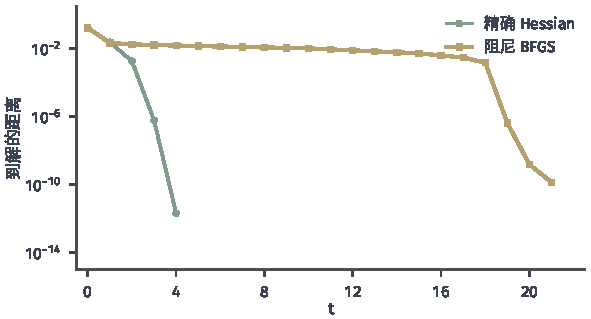
\includegraphics[width=100mm]{figures/05-optimization/06-constrained-optimization/matplotlib/sqp-exact-bfgs-rate/figure.pdf}
 \caption{五变量问题上到解的距离。绿线是精确Lagrange Hessian的全步长SQP，黄线是阻尼BFGS加罚函数回溯。两者起点相同，后者每轮不需要二阶导数。}
 \label{fig:sqp-exact-bfgs-rate}
\end{BookInlineFigure}

这个对比只是一个例子，轮数的差距随问题而变。局部速度的结论还需要曲率近似的条件。记$\bm{P}^{(t)}$是向$\bm{A}^{(t)}$零空间的投影，$\bm{H}_{\mathcal{L}}^\star$是Lagrange函数在解处对$\bm{x}$的Hessian，需要的条件是
\begin{equation}
 \lim_{t\to\infty}\frac{\lVert\bm{P}^{(t)}\bigl(\bm{B}^{(t)}-\bm{H}_{\mathcal{L}}^\star\bigr)\bm{d}^{(t)}\rVert_2}{\lVert\bm{d}^{(t)}\rVert_2}=0.
 \label{eq:sqp-dennis-more}
\end{equation}
它只要求沿步的方向、在切空间内近似准确，不要求$\bm{B}^{(t)}$收敛到真实的Hessian。这一点很重要，因为$\bm{H}_{\mathcal{L}}^\star$可以不定，而正定的BFGS矩阵无法趋于不定矩阵；在切空间上$\bm{H}_{\mathcal{L}}^\star$却是正定的，式~\eqref{eq:sqp-dennis-more}仍可能成立。

\section{更新的接受}
\label{sec:sqp-acceptance}

QP给出的步只在模型里是好的。把步放回非线性问题，凭什么判断它值得采用？

无约束时这个问题很简单，看目标有没有下降。约束问题有两个指标。第~\ref{sec:sqp-equality-qp}节的第三步目标从$-2.0588$升到$-2.0009$，约束违反却从$0.119$降到$0.0018$；而从圆上的点$(1.4,0.2)^\top$走一个全步，目标从$-1.6$降到$-2.32$，违反量却从$0$升到$0.72$。两个指标常常冲突，必须有一条明确规则来评价进展。第~\ref{sec:sqp-merit}小节把两者压成一个数，第~\ref{sec:sqp-filter}小节把两者并排比较。

记约束的总违反量为
\begin{equation}
 \theta(\bm{x})=\sum_{j=1}^p\lvert h_j(\bm{x})\rvert+\sum_{i=1}^m[g_i(\bm{x})]_+,
 \label{eq:sqp-violation}
\end{equation}
其中$[u]_+=\max\{u,0\}$。

\subsection{罚函数线搜索}
\label{sec:sqp-merit}

\paragraph{评价函数}
把目标和违反量加起来，用一个权重$\rho>0$换算两者的单位，得到
\begin{equation}
 \phi_\rho(\bm{x})=f(\bm{x})+\rho\,\theta(\bm{x}).
 \label{eq:sqp-merit}
\end{equation}
这是第~\ref{chap:penalty-multiplier-methods}章的$\ell_1$精确惩罚函数，在这里它的角色是判断步的好坏，称为\term{评价函数}（merit function）。那一章的结论是：若$\bm{x}^\star$满足二阶充分条件，且权重大于乘子的最大绝对值，则$\bm{x}^\star$是$\phi_\rho$的严格局部最小点。乘子是约束的影子价格，权重就是愿意为单位违反付的罚款，罚款低于影子价格，违约反而划算。

$\phi_\rho$在$h_j=0$或$g_i=0$处不可微，但沿任意方向的方向导数存在。记$D(\phi_\rho;\bm{d})$为它在$\bm{x}^{(t)}$处沿$\bm{d}$的方向导数。下面的引理告诉我们，QP的解在什么时候是下降方向。

\begin{lemma}[QP步的下降性]
\label{lem:sqp-merit-descent}
设$(\bm{d},\hat{\bm{\lambda}},\hat{\bm{\nu}})$满足条件~\eqref{eq:sqp-qp-kkt}，则
\begin{equation}
 D(\phi_\rho;\bm{d})\leq-\bm{d}^\top\bm{B}^{(t)}\bm{d}-\bigl(\rho-\max\{\lVert\hat{\bm{\nu}}\rVert_\infty,\lVert\hat{\bm{\lambda}}\rVert_\infty\}\bigr)\theta(\bm{x}^{(t)}).
 \label{eq:sqp-merit-descent}
\end{equation}
\end{lemma}

\begin{proof}
分别计算$\theta$和$f$的方向导数。先看等式项。线性化约束给出$\langle\nabla h_j,\bm{d}\rangle=-h_j$。若$h_j\neq0$，则$\lvert h_j\rvert$的方向导数是$h_j$的符号乘以$\langle\nabla h_j,\bm{d}\rangle$，等于$-\lvert h_j\rvert$；若$h_j=0$，则$\langle\nabla h_j,\bm{d}\rangle=0$，方向导数为$0$。两种情况都等于$-\lvert h_j\rvert$。

再看不等式项，线性化约束给出$\langle\nabla g_i,\bm{d}\rangle\leq-g_i$。若$g_i>0$，$[g_i]_+$的方向导数是$\langle\nabla g_i,\bm{d}\rangle\leq-[g_i]_+$；若$g_i=0$，方向导数是$[\langle\nabla g_i,\bm{d}\rangle]_+=0$；若$g_i<0$，方向导数是$0$。三种情况都不超过$-[g_i]_+$。把这些加起来，得到
\[
 D(\theta;\bm{d})\leq-\theta(\bm{x}^{(t)}).
\]

然后看目标。用$\bm{d}^\top$左乘式~\eqref{eq:sqp-qp-kkt}第一行，再用线性化约束和互补条件换掉$\bm{A}\bm{d}$和$\bm{G}\bm{d}$：
\[
 \begin{aligned}
 \langle\nabla f,\bm{d}\rangle
 &=-\bm{d}^\top\bm{B}\bm{d}-\hat{\bm{\nu}}^\top\bm{A}\bm{d}-\hat{\bm{\lambda}}^\top\bm{G}\bm{d}\\
 &=-\bm{d}^\top\bm{B}\bm{d}+\hat{\bm{\nu}}^\top\bm{h}+\hat{\bm{\lambda}}^\top\bm{g}.
 \end{aligned}
\]

最后估计两个内积。第一个用Hölder不等式，第二个先用$\hat{\bm{\lambda}}\geq\bm{0}$把$\bm{g}$放大成$[\bm{g}]_+$，再用Hölder不等式：
\[
 \begin{aligned}
 \hat{\bm{\nu}}^\top\bm{h}&\leq\lVert\hat{\bm{\nu}}\rVert_\infty\lVert\bm{h}\rVert_1,\\
 \hat{\bm{\lambda}}^\top\bm{g}&\leq\hat{\bm{\lambda}}^\top[\bm{g}]_+\leq\lVert\hat{\bm{\lambda}}\rVert_\infty\lVert[\bm{g}]_+\rVert_1.
 \end{aligned}
\]

合起来，
\[
 \langle\nabla f,\bm{d}\rangle\leq-\bm{d}^\top\bm{B}\bm{d}+\max\{\lVert\hat{\bm{\nu}}\rVert_\infty,\lVert\hat{\bm{\lambda}}\rVert_\infty\}\,\theta(\bm{x}^{(t)}).
\]
$\phi_\rho$的方向导数是$\langle\nabla f,\bm{d}\rangle$与$\rho D(\theta;\bm{d})$之和，式~\eqref{eq:sqp-merit-descent}成立。
\end{proof}

引理说明，当$\rho$超过QP乘子的最大绝对值，并且$\bm{d}^\top\bm{B}\bm{d}$为正时，$\bm{d}$是$\phi_\rho$的下降方向。这里的正性只需在$\bm{d}$上成立。$\bm{d}^\top\bm{B}\bm{d}$可能为负时，条件要通过第~\ref{sec:sqp-curvature}节的修正来保证。

\paragraph{权重的两难}
式~\eqref{eq:sqp-merit-descent}要求$\rho$足够大，但$\rho$并不是越大越好。看问题~\eqref{eq:sqp-circle}沿射线$x_1=x_2=s$的情形，此时
\[
 \phi_\rho(s,s)=-2s+\rho\,\lvert2s^2-2\rvert.
\]

在$s>1$上，$\phi_\rho$的导数是$-2+4\rho s$。$\rho=0.1$时导数在$s=5$才变号，评价函数在$(5,5)$有局部最小值，其值$-5.2$比解处的$-2$还小。沿着$\phi_{0.1}$下降会被带到严重违约的地方。

$s=1$处的右导数是$-2+4\rho$，要它为正需要$\rho>1/2=\nu^\star$，这正是权重要超过乘子的具体含义。图~\ref{fig:sqp-merit-rho-ray}比较了三种权重。权重过大时，$\phi_\rho$在约束面两侧形成很陡的峡谷，任何离开约束面的步，即使只离开$\lVert\bm{d}\rVert_2^2$这么多，也要付很高的代价，步长于是被压得很小，迭代只能贴着约束面慢慢挪。

\begin{BookInlineFigure}
 \centering
 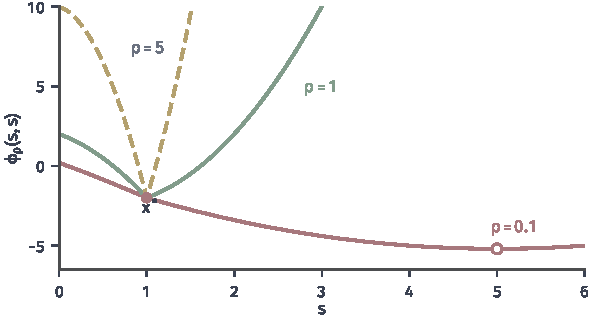
\includegraphics[width=100mm]{figures/05-optimization/06-constrained-optimization/matplotlib/sqp-merit-rho-ray/figure.pdf}
 \caption{评价函数沿射线$x_1=x_2=s$的形状。红线$\rho=0.1$低于乘子，空心点$(5,5)$是错误的局部最小点；绿线$\rho=1$在解$s=1$（红点）处形成拐点；黄色虚线$\rho=5$的峡谷很陡。}
 \label{fig:sqp-merit-rho-ray}
\end{BookInlineFigure}

实际算法动态调整权重。常用规则是每轮令$\rho$不小于当前QP乘子的最大绝对值再加一个裕量$\delta>0$：
\begin{equation}
 \rho^{(t)}\geq\max\{\lVert\hat{\bm{\nu}}\rVert_\infty,\lVert\hat{\bm{\lambda}}\rVert_\infty\}+\delta.
 \label{eq:sqp-rho-rule}
\end{equation}
权重只升不降时，迭代的后期可能一直背着远离解时抬高的权重，因此实现中也允许有控制地下调。

\paragraph{主要思想}
有了下降方向，就和无约束问题一样回溯。从$\alpha=1$开始试，直到满足充分下降条件：
\begin{equation}
 \phi_\rho(\bm{x}^{(t)}+\alpha\bm{d}^{(t)})\leq\phi_\rho(\bm{x}^{(t)})+\eta\,\alpha\,D(\phi_\rho;\bm{d}^{(t)}),
 \label{eq:sqp-armijo}
\end{equation}
其中$\eta\in(0,1/2)$。由于$\phi_\rho$沿$\bm{d}$在$\alpha=0$右侧的导数就是$D$，小的$\alpha$总能满足这个条件。

\needspace{6\baselineskip}
\paragraph{变量}
\begin{itemize}
 \item $\bm{x}^{(t)}$、$\bm{\nu}^{(t)}$：当前点与乘子；$\rho$：评价函数的权重。
 \item $\bm{d}^{(t)}$、$\hat{\bm{\nu}}$：QP的解与乘子；$D$：$\phi_\rho$的方向导数。
 \item $\eta$：充分下降系数；$\alpha^{(t)}$：接受的步长。
\end{itemize}

\paragraph{初始化}
给定$\bm{x}^{(0)}$、$\bm{\nu}^{(0)}$、$\rho$和$\eta$。例中取圆上的一点，数据是
\[
 \bm{x}^{(0)}=(1.4,\ 0.2)^\top,\qquad\nu^{(0)}=0.5,\qquad\rho=2,\qquad\eta=0.1.
\]
这里$h(\bm{x}^{(0)})=1.96+0.04-2=0$，点是可行的，$\phi_\rho(\bm{x}^{(0)})=-1.6$。

\needspace{6\baselineskip}
\paragraph{每轮更新}
\begin{enumerate}
 \item 解QP得$\bm{d}^{(t)}$和乘子。例中第一轮$\bm{B}=\bm{I}$，$\bm{A}=(2.8,0.4)$，$h=0$，解得
 \[
  \hat\nu=0.4,\qquad\bm{d}^{(0)}=(-0.12,\ 0.84)^\top.
 \]

 \item 按需要增大$\rho$，并计算方向导数，即$D=\langle\nabla f,\bm{d}\rangle-\rho\,\theta$（只含等式时）。例中$\rho=2\geq\hat\nu$，$\theta=0$，于是
 \[
  D=\langle(-1,-1)^\top,\bm{d}^{(0)}\rangle=-0.72.
 \]

 \item 令$\alpha=1$，当式~\eqref{eq:sqp-armijo}不成立时令$\alpha\leftarrow\alpha/2$。例中沿$\bm{d}$有$h(\bm{x}+\alpha\bm{d})=0.72\alpha^2$，$f(\bm{x}+\alpha\bm{d})=-1.6-0.72\alpha$，所以
 \[
  \phi_\rho(\alpha)=-1.6-0.72\,\alpha+1.44\,\alpha^2.
 \]

 依次试三个步长，每个步长下左边是$\phi_\rho$的值，右边是式~\eqref{eq:sqp-armijo}的门槛：
 \[
  \begin{aligned}
  \alpha=1:&\quad-0.88>-1.672,\\
  \alpha=0.5:&\quad-1.6>-1.636,\\
  \alpha=0.25:&\quad-1.69\leq-1.618.
  \end{aligned}
 \]
 前两个被拒绝，第三个被接受，图~\ref{fig:sqp-merit-armijo}画出了这三次试探。

 \item 更新迭代点，乘子按式~\eqref{eq:sqp-multiplier-update}。例中第一轮
 \[
  \bm{x}^{(1)}=(1.37,\ 0.41)^\top,\qquad\nu^{(1)}=0.5+0.25\,(0.4-0.5)=0.475.
 \]

 第二轮$h=0.045$，$\bm{d}^{(1)}\approx(-0.21767,0.67247)^\top$，$\alpha^{(1)}=0.25$；第三轮$\alpha^{(2)}=0.5$；第四轮起$\alpha^{(t)}=1$。

 \item 按第~\ref{sec:sqp-convergence}节的残差判断是否停止。
\end{enumerate}

最终$\bm{x}^{(t)}$到达$(1,1)^\top$，例中$t=6$时到解的距离已低于$10^{-6}$。

\begin{BookInlineFigure}
 \centering
 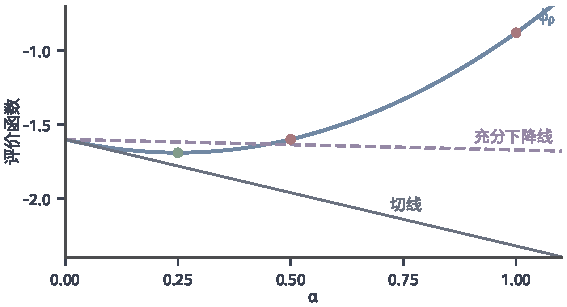
\includegraphics[width=96mm]{figures/05-optimization/06-constrained-optimization/matplotlib/sqp-merit-armijo/figure.pdf}
 \caption{从$\bm{x}^{(0)}=(1.4,0.2)^\top$沿QP步的评价函数，$\rho=2$。蓝线是$\phi_\rho(\alpha)$，灰线是切线，紫色虚线是充分下降的门槛。红点$\alpha=1$与$\alpha=0.5$被拒绝，绿点$\alpha=0.25$被接受。}
 \label{fig:sqp-merit-armijo}
\end{BookInlineFigure}

这个例子还暗示了一个毛病。全步到达$(1.28,1.04)^\top$，到解的距离从$0.894$缩到$0.283$，明明很好，评价函数却把它拒绝了。原因及补救在第~\ref{sec:sqp-soc}小节。

\paragraph{用信赖域代替线搜索}
线搜索固定方向、调整步长。也可以用第~\ref{chap:trust-region}章的方式固定一个半径，比较实际下降与模型预测，比值大则接受并放大半径，比值小则缩小半径。线性化的约束有可能与半径冲突，所以需要第~\ref{sec:sqp-hessian-modification}小节提到的法向段与切向段的安排。信赖域版本可以自然处理负曲率，代价是实现更复杂。

\subsection{过滤器}
\label{sec:sqp-filter}

罚函数要预先定一个换算比例。本小节要回答的问题是：能不能不做这个换算，直接比较$\theta$和$f$这两个指标？

\paragraph{基本想法}
类比两人比赛：如果候选步在两个指标上都比某个历史记录差，就没有接受的理由；只要在某个指标上比所有记录都更好，就给它一个机会。把已接受的点的$(\theta,f)$对存下来，这个集合称为\term{过滤器}（filter），记为$\mathcal{F}$。

如果只要求“不被支配”，也就是不被某条记录在两个指标上同时压过，算法可能无限地取得微不足道的进步。设想$\theta$的序列是$1+1/k$，每一项都比前一项略小，$f$保持不变，每一步都不被支配，极限却是$\theta=1$，一个不可行的点。所以真正的条件要带裕量。

\begin{definition}[过滤器的接受条件]
\label{def:sqp-filter}
给定$\gamma\in(0,1)$，候选点$\bm{x}^{+}$可被过滤器$\mathcal{F}$接受，是指对每条记录$(\theta_l,f_l)\in\mathcal{F}$，都有
\begin{equation}
 \theta(\bm{x}^{+})\leq(1-\gamma)\,\theta_l\quad\text{或}\quad f(\bm{x}^{+})\leq f_l-\gamma\,\theta_l.
 \label{eq:sqp-filter}
\end{equation}
\end{definition}

条件的后半式里的裕量是$\gamma\theta_l$，它与违反量成比例。这样一来，要么约束违反按比例减小，要么目标确实下降一段距离，前面那个微小进步的序列不再能被接受。

用一组教学数据演示。取$\gamma=0.1$，三条记录为
\[
 (\theta_1,f_1)=(0.8,-2.6),\quad(\theta_2,f_2)=(0.3,-2.2),\quad(\theta_3,f_3)=(0.05,-1.9).
\]

候选点$A=(0.2,-2.4)$：对记录一，$0.2\leq0.72$；对记录二，$0.2\leq0.27$；对记录三，$\theta$不够小，但目标满足$-2.4\leq-1.905$。三条都通过，接受。

候选点$B=(0.4,-2.0)$：对记录一通过；对记录二，$0.4>0.27$，目标$-2.0>-2.23$，失败，拒绝。

候选点$C=(0.295,-2.205)$看上去比记录二好一点，$\theta$和$f$都略小。但$0.295>0.27$，$-2.205>-2.23$，改进不够裕量，同样拒绝。图~\ref{fig:sqp-filter-plane}是这三个点的位置。

\begin{BookInlineFigure}
 \centering
 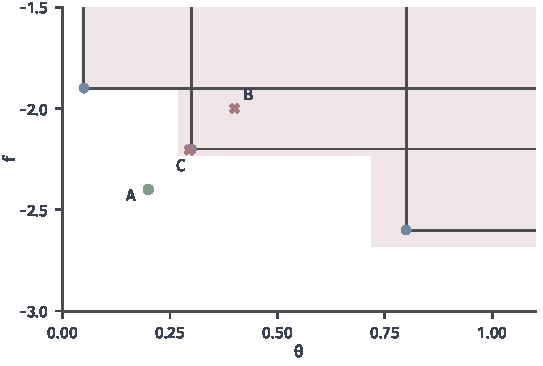
\includegraphics[width=92mm]{figures/05-optimization/06-constrained-optimization/matplotlib/sqp-filter-plane/figure.pdf}
 \caption{过滤器的$(\theta,f)$平面，蓝点是三条记录，深灰线是它们支配的范围边界，红色浅底是带裕量$\gamma=0.1$的禁止区。绿点$A$被接受，红叉$B$和$C$被拒绝，其中$C$虽不被支配，但在裕量带内。}
 \label{fig:sqp-filter-plane}
\end{BookInlineFigure}

\paragraph{还需要什么}
只靠式~\eqref{eq:sqp-filter}并不足以保证收敛到KKT点。还要回答三件事。

第一，局部切换。若迭代点已经几乎可行，而模型预测目标有明显下降，就不能只凭$\theta$有所改善就接受，要转而要求目标满足类似式~\eqref{eq:sqp-armijo}的充分下降，这样的步也不写入过滤器。否则算法可能收敛到一个可行但并不最优的点。

第二，什么时候写入记录。不满足上述切换条件而被接受的步，把当前点的$(\theta,f)$写入过滤器，并删去被它支配的旧记录。这样禁止区只会扩大，同一区域不会被反复光顾。

第三，可行性恢复。回溯到很小的步长仍无法被接受，说明当前的线性化方向帮不上忙，这时转入下一节的恢复阶段。过滤器不能代替这些规则。

表~\ref{tab:sqp-merit-filter}总结了两种规则。

\begin{BookInlineTable}
 \centering
 \begin{tabular}{lll}
  \toprule
  比较项 & 罚函数 & 过滤器\\
  \midrule
  进展的度量 & 一个数$\phi_\rho$ & 两个数$(\theta,f)$\\
  需要的参数 & 权重$\rho$ & 裕量$\gamma$、切换常数\\
  主要风险 & $\rho$太小或太大 & 需额外的恢复与切换\\
  历史信息 & 不保存 & 保存记录\\
  \bottomrule
 \end{tabular}
 \caption{罚函数线搜索与过滤器的比较。}
 \label{tab:sqp-merit-filter}
\end{BookInlineTable}

\section{模型的修复}
\label{sec:sqp-repair}

前面两节都假定子问题有解，候选步也还算合用。本节处理两种不成立的情形，要回答的问题是：失败发生在哪一层，相应地该修什么？第一种失败发生在子问题上，线性化约束根本没有可行解，此时缩小步长毫无用处，因为连可以缩小的步都不存在。第二种失败发生在候选步上，QP有解，步却被真实约束的弯曲挡住。

图~\ref{fig:sqp-repair-tree}按失败原因列出修复手段。只靠反复缩小步长处理所有问题，第一种情形无效，第二种情形则会拖慢收敛。

\begin{BookInlineFigure}
 \centering
 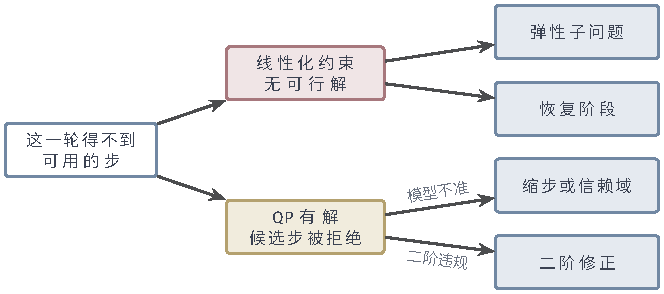
\includegraphics[width=112mm]{figures/05-optimization/06-constrained-optimization/tikz/sqp-repair-tree/figure.pdf}
 \caption{得不到可用的步时的两类原因及其修复。红框是子问题层面的失败，黄框是候选步层面的失败，蓝框是对应的处理。}
 \label{fig:sqp-repair-tree}
\end{BookInlineFigure}

\subsection{可行性恢复}
\label{sec:sqp-restoration}

\paragraph{线性化约束可能相互矛盾}
原问题可行，并不意味着它的线性化可行。看下面的问题：
\begin{equation}
 \min_{\bm{x}}\ \frac12\bigl((x_1-2)^2+x_2^2\bigr)
 \quad\text{s.t.}\quad h_1=x_2-x_1^2=0,\quad h_2=x_2-1=0.
 \label{eq:sqp-inconsistent}
\end{equation}
可行点只有$(\pm1,1)^\top$，解是$\bm{x}^\star=(1,1)^\top$。从原点出发，约束的值和Jacobian是
\[
 \bm{h}^{(0)}=(0,-1)^\top,\qquad\bm{A}^{(0)}=\begin{bmatrix}0&1\\0&1\end{bmatrix}.
\]

线性化约束成为$d_2=0$和$d_2=1$，两者矛盾。抛物线在顶点的切线是水平的，与直线$x_2=1$平行，图~\ref{fig:sqp-inconsistent}(a)里两条线永不相交。这里$\bm{A}^{(0)}$的秩为$1$，定理~\ref{thm:sqp-eqp}的前提失效。

\begin{BookInlineFigure}
 \centering
 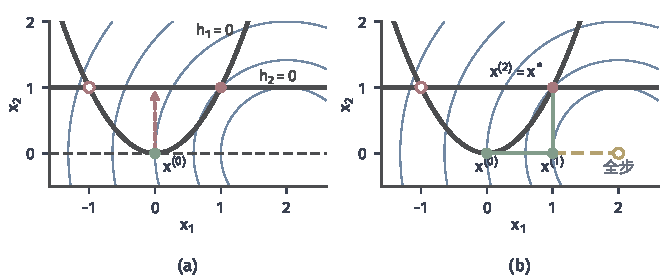
\includegraphics[width=112mm]{figures/05-optimization/06-constrained-optimization/matplotlib/sqp-inconsistent/figure.pdf}
 \caption{问题~\eqref{eq:sqp-inconsistent}。深灰粗线是抛物线$h_1=0$和直线$h_2=0$，蓝线是目标的等高线，红点是解，空心点是另一个可行点。(a)~原点处抛物线的线性化（虚线）与$h_2=0$平行，红色箭头表示两者之间的距离无法消除。(b)~弹性子问题的全步到$(2,0)^\top$（黄色虚线），回溯到一半得$\bm{x}^{(1)}$，下一轮的QP相容，一步到解。}
 \label{fig:sqp-inconsistent}
\end{BookInlineFigure}

\paragraph{弹性子问题}
第一种修复是让约束可以有偿违反。给每条线性化约束加上非负的松弛变量，并在目标中按权重$\rho$收费，得到\term{弹性子问题}（elastic subproblem）：
\begin{equation}
 \begin{aligned}
 \min_{\bm{d},\bm{v},\bm{w},\bm{u}}\quad & \langle\nabla f,\bm{d}\rangle+\frac12\bm{d}^\top\bm{B}\bm{d}
 +\rho\bigl(\langle\bm{1},\bm{v}+\bm{w}\rangle+\langle\bm{1},\bm{u}\rangle\bigr)\\
 \text{s.t.}\quad & \bm{h}+\bm{A}\bm{d}=\bm{v}-\bm{w},\\
 & \bm{g}+\bm{G}\bm{d}\leq\bm{u},\\
 & \bm{v},\bm{w},\bm{u}\geq\bm{0}.
 \end{aligned}
 \label{eq:sqp-elastic}
\end{equation}
它对任何数据都可行，取$\bm{d}=\bm{0}$，松弛变量等于当前的违反量即可。

消去松弛变量，式~\eqref{eq:sqp-elastic}就是在线性化约束上最小化$\ell_1$惩罚的模型。第~\ref{chap:penalty-multiplier-methods}章的精确惩罚论证用在这个凸QP上，得到：当线性化约束相容且$\rho$大于QP乘子的最大绝对值时，松弛变量全为零，弹性解就是原来QP的解。所以可以总是求解弹性形式，不必先判断QP是否可行。

例中取$\bm{B}^{(0)}=\bm{I}$，$\rho=1$。$\nabla f=(-2,0)^\top$，消去松弛变量后，模型是
\[
 -2d_1+\frac12d_1^2+\frac12d_2^2+\lvert d_2\rvert+\lvert d_2-1\rvert.
\]

对$d_1$的最小化独立于$d_2$，得$d_1=2$。在$0\leq d_2\leq1$上两个绝对值之和恒为$1$，这个区间内只剩$\frac12d_2^2$起作用，所以$d_2=0$。于是
\[
 \bm{d}^{(0)}=(2,\ 0)^\top,\qquad\text{模型中的违反量}=1.
\]

这一步并没有修好$h_2$，只是把目标朝$x_1$方向推。候选点要用真实函数检验。起点的评价函数是$\phi_1(\bm{0})=2+1=3$，全步的值和半步的值分别是
\[
 \phi_1(2,0)=0+4+1=5,\qquad\phi_1(1,0)=0.5+1+1=2.5.
\]

全步因线性化高估而被拒绝，半步通过。于是$\bm{x}^{(1)}=(1,0)^\top$。这里$h_1=-1$，梯度变成$(-2,1)$，第一行不再与第二行平行，线性化约束变成
\[
 -1-2d_1+d_2=0,\qquad-1+d_2=0.
\]

它有唯一解$\bm{d}^{(1)}=(0,1)^\top$，下一点恰好就是$(1,1)^\top$。这里能一步到解有偶然的成分，两个约束两个变量，线性化解恰好落在抛物线上。要点是离开奇异点之后，线性化又恢复了相容，图~\ref{fig:sqp-inconsistent}(b)是这条路径。

\paragraph{恢复阶段}
第二种修复更彻底。暂时不管$f$，改而求解只关心可行性的问题：
\begin{equation}
 \min_{\bm{x}}\ \theta(\bm{x}).
 \label{eq:sqp-restoration}
\end{equation}
这称为\term{可行性恢复}（feasibility restoration）。当回溯到很小的步长仍不被过滤器或评价函数接受，或者弹性子问题的松弛变量长期不为零时，就转入恢复阶段。

恢复阶段的目标与原优化目标不同，这是必须记住的。它不保证目标下降，甚至可能把目标抬得很高。一旦违反量明显减小，并且新点能被过滤器接受或线性化重新相容，就停止恢复，在新点重建SQP模型，回到原来的目标上。

\paragraph{恢复失败说明不了什么}
恢复阶段可能停在$\theta$的局部最小点，而$\theta$在那里仍然为正。这能证明原问题无可行解吗？不能。看单变量约束
\[
 h(x)=x^3-3x+3=0.
\]

$h'(x)=3x^2-3$在$x=1$处为零，且$h(1)=1>0$，所以$x=1$是$\lvert h\rvert$的局部最小点。从$x=1$附近出发的恢复过程会困在这里，而方程在$x\approx-2.104$有实根。局部方法看到的只是局部信息，它只能报告“在这里找不到可行点”，要证明不可行需要全局的论证或对偶证书。

\subsection{二阶修正（补充）}
\label{sec:sqp-soc}

第~\ref{sec:sqp-merit}小节留下一个疑点：好的全步被评价函数拒绝。本小节要回答的问题是：这种误判从何而来，怎样在不放弃这个步的前提下消除它？

\paragraph{好步被拒绝}
下面的问题是弯曲约束上的典型例子：
\begin{equation}
 \min_{\bm{x}}\ 2(x_1^2+x_2^2-1)-x_1
 \quad\text{s.t.}\quad h=x_1^2+x_2^2-1=0.
 \label{eq:sqp-maratos}
\end{equation}
解是$\bm{x}^\star=(1,0)^\top$，在此处驻定条件$(3,0)^\top+\nu(2,0)^\top=\bm{0}$给出$\nu^\star=-3/2$。取$\nu=\nu^\star$，于是$\bm{B}=(4+2\nu)\bm{I}=\bm{I}$。

取圆上的点$\bm{x}=(0.8,0.6)^\top$，此时$h=0$，$f=-0.8$，梯度和Jacobian是
\[
 \nabla f=(2.2,\ 2.4)^\top,\qquad\bm{A}=(1.6,\ 1.2).
\]

解KKT系统。用$\bm{A}$左乘第一行并用$\bm{A}\bm{d}=0$，由$\bm{A}\nabla f=6.4$和$\bm{A}\bm{A}^\top=4$得$\hat\nu=-1.6$，于是
\[
 \bm{d}=(0.36,\ -0.48)^\top,\qquad\bm{x}+\bm{d}=(1.16,\ 0.12)^\top.
\]

这一步很好：到解的距离从$0.632$缩短到$0.2$。可是真实函数值都变差了：
\[
 f(\bm{x}+\bm{d})=-0.44>-0.8,\qquad h(\bm{x}+\bm{d})=0.36>0.
\]

目标上升，违反量也上升，对任何$\rho>0$，$\phi_\rho$都升高了，这一步被拒绝。过滤器同样拒绝，因为记录$(0,-0.8)$在两个指标上都压过候选$(0.36,-0.44)$。这种现象称为\term{Maratos效应}（Maratos effect）：全步本可带来快速的局部收敛，却被接受规则判为失败，迫使算法缩短步长，收敛变慢。

原因在于约束的弯曲。线性化保证$\bm{A}\bm{d}=-\bm{h}$，但二阶项留在了约束上，$h(\bm{x}+\bm{d})=\lVert\bm{d}\rVert_2^2=0.36$。这个二阶大小的违反，足以抵消模型预期的目标下降。Lagrange函数其实是下降的，目标的增量$0.36$加上$\nu^\star$乘约束的增量$0.36$，合计是$-0.18$。评价函数中$\ell_1$项的绝对值把这一点丢掉了。

\paragraph{补一个修正步}
既然问题是二阶的违反，就补一步把它修掉。在$\bm{x}+\bm{d}$处重新计算约束的值，但沿用当前的Jacobian，求一个最小范数的修正：
\begin{equation}
 \hat{\bm{d}}=-\bm{A}^\top\bigl(\bm{A}\bm{A}^\top\bigr)^{-1}\bm{h}(\bm{x}+\bm{d}).
 \label{eq:sqp-soc}
\end{equation}
然后用$\bm{x}+\bm{d}+\hat{\bm{d}}$作候选点，这称为\term{二阶修正}（second-order correction）。

例中$\bm{A}\bm{A}^\top=4$，$h(\bm{x}+\bm{d})=0.36$，代入式~\eqref{eq:sqp-soc}，得
\[
 \hat{\bm{d}}=-(1.6,\ 1.2)^\top\times0.09=(-0.144,\ -0.108)^\top.
\]

修正后的候选点及其函数值是
\[
 \bm{x}+\bm{d}+\hat{\bm{d}}=(1.016,\ 0.012)^\top,\quad h=0.0324,\quad f=-0.9512.
\]

现在$\rho=2$时评价函数的值是$-0.9512+0.0648=-0.8864$，低于$-0.8$，步被接受，到解的距离只有$0.02$。过滤器也接受它，因为目标已满足$-0.9512\leq-0.8$。图~\ref{fig:sqp-maratos}(a)是这两段，(b)是整个迭代的比较。

\begin{BookInlineFigure}
 \centering
 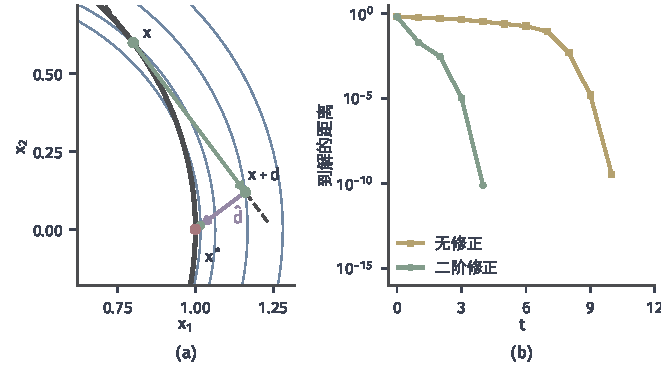
\includegraphics[width=112mm]{figures/05-optimization/06-constrained-optimization/matplotlib/sqp-maratos/figure.pdf}
 \caption{问题~\eqref{eq:sqp-maratos}上的Maratos效应与二阶修正。(a)~深灰粗线是约束，蓝线是目标的等高线，虚线是线性化约束；绿色箭头是QP步，紫色箭头是修正步$\hat{\bm{d}}$，红点是解。(b)~$\rho=2$、$\eta=0.1$的回溯SQP：不修正（黄）前七轮步长被缩短，修正（绿）后每轮都走全步。}
 \label{fig:sqp-maratos}
\end{BookInlineFigure}

\paragraph{为什么修正是二阶的}
设$\lVert\bm{d}\rVert_2$很小。约束在$\bm{x}+\bm{d}$处的值只剩二阶项，所以$\hat{\bm{d}}$的长度是$\lVert\bm{d}\rVert_2^2$的量级，比主步小一阶，不会破坏主步带来的快速收敛。

把修正后的点代入约束展开，$\bm{A}(\bm{x}+\bm{d})$与$\bm{A}(\bm{x})$之差是$\lVert\bm{d}\rVert_2$的量级，乘以$\hat{\bm{d}}$得三阶项；其余项也是三阶以上，因此修正后的违反量降到$\lVert\bm{d}\rVert_2^3$的量级。

\paragraph{与重新解QP的区别}
修正步用的是已有的$\bm{A}$和它的分解，只换了右端，代价是一次回代加一次约束求值。重新构造并求解QP则要重新求导和分解。有不等式时，修正要在主步的工作集上做，或者把线性化约束的常数项换成$\bm{g}(\bm{x}+\bm{d})-\bm{G}\bm{d}$再解一次QP，后者花费更多，但结果仍是原QP的一次扰动。

实现中通常只在全步被拒绝、且约束违反确实增加时才试一次修正，试探失败就回到回溯。也有别的办法绕开Maratos效应，例如暂时放行一步、几步之后再回头检查的非单调策略，以及改用可微的评价函数。

\section{收敛与计算成本}
\label{sec:sqp-convergence}

各个部件都有了，本节回答三个问题：在解附近能收敛多快，什么时候算结束，以及每一轮的计算花在哪里。

\paragraph{精确Hessian的局部二次收敛}
先看只含等式的情形，记$\bm{w}=(\bm{x},\bm{\nu})$。定理~\ref{thm:sqp-newton}说全步长SQP就是$\bm{F}(\bm{w})=\bm{0}$上的Newton法，其Jacobian正是KKT矩阵$\bm{K}(\bm{w})$。所以收敛性的证明与第~\ref{chap:second-order-methods}章的证明思路相同，只是矩阵不再对称正定。

\begin{theorem}[SQP的局部二次收敛]
\label{thm:sqp-local-quadratic}
设$\bm{w}^\star=(\bm{x}^\star,\bm{\nu}^\star)$满足等式约束问题的KKT条件，$\bm{A}(\bm{x}^\star)$行满秩，并且$\nabla^2_{\bm{x}\bm{x}}\mathcal{L}(\bm{w}^\star)$在$\bm{A}(\bm{x}^\star)$的零空间上正定。设在半径为$r$的球内$\bm{K}$满足
\begin{equation}
 \lVert\bm{K}(\bm{w})-\bm{K}(\bm{w}')\rVert_2\leq M\lVert\bm{w}-\bm{w}'\rVert_2.
 \label{eq:sqp-k-lipschitz}
\end{equation}
令$\sigma>0$为$\bm{K}(\bm{w}^\star)$的最小奇异值。若$\lVert\bm{w}^{(t)}-\bm{w}^\star\rVert_2<\min\{r,\sigma/(2M)\}$，则全步长SQP的下一点有定义，且
\begin{equation}
 \lVert\bm{w}^{(t+1)}-\bm{w}^\star\rVert_2\leq\frac{M}{\sigma}\lVert\bm{w}^{(t)}-\bm{w}^\star\rVert_2^2.
 \label{eq:sqp-quadratic-bound}
\end{equation}
\end{theorem}

\begin{proof}
记$\bm{e}=\bm{w}^{(t)}-\bm{w}^\star$，$\bm{K}=\bm{K}(\bm{w}^{(t)})$。定理~\ref{thm:sqp-eqp}说明$\bm{K}(\bm{w}^\star)$可逆，所以$\sigma>0$。

第一步说明$\bm{K}$的逆有界。由式~\eqref{eq:sqp-k-lipschitz}，
\[
 \lVert\bm{K}-\bm{K}(\bm{w}^\star)\rVert_2\leq M\lVert\bm{e}\rVert_2\leq\frac\sigma2.
\]
最小奇异值的扰动不超过矩阵差的范数，所以$\bm{K}$的最小奇异值至少是$\sigma/2$，即
\[
 \lVert\bm{K}^{-1}\rVert_2\leq\frac2\sigma.
\]

第二步写出误差递推。由$\bm{F}(\bm{w}^\star)=\bm{0}$沿线段积分，
\[
 \bm{F}(\bm{w}^{(t)})=\int_0^1\bm{K}(\bm{w}^\star+s\bm{e})\bm{e}\,\mathrm{d}s.
\]

下一点是$\bm{w}^{(t)}$减去$\bm{K}^{-1}\bm{F}(\bm{w}^{(t)})$，把上式代入，得到
\[
 \bm{w}^{(t+1)}-\bm{w}^\star
 =\bm{K}^{-1}\int_0^1\bigl(\bm{K}-\bm{K}(\bm{w}^\star+s\bm{e})\bigr)\bm{e}\,\mathrm{d}s.
\]

第三步估计积分。由式~\eqref{eq:sqp-k-lipschitz}，被积函数的范数不超过$M(1-s)\lVert\bm{e}\rVert_2^2$，积分后得
\[
 \Bigl\lVert\int_0^1\bigl(\bm{K}-\bm{K}(\bm{w}^\star+s\bm{e})\bigr)\bm{e}\,\mathrm{d}s\Bigr\rVert_2\leq\frac M2\lVert\bm{e}\rVert_2^2.
\]
再乘以第一步的界，式~\eqref{eq:sqp-quadratic-bound}成立。
\end{proof}

这里$M$是$\bm{K}$的Lipschitz常数，它由$f$与$h_j$的三阶导数大小和乘子的大小共同决定，当目标和约束的Hessian都Lipschitz连续时存在。由于$\lVert\bm{e}\rVert_2<\sigma/(2M)$时式~\eqref{eq:sqp-quadratic-bound}的右端小于$\lVert\bm{e}\rVert_2/2$，迭代留在球内，二次收敛一直保持。

条件各有用处。行满秩和约化曲率正定都是用来保证$\bm{K}(\bm{w}^\star)$可逆的，这正是定理~\ref{thm:sqp-eqp}的条件。注意结论是关于$\bm{w}$的。单看$\bm{x}$的误差，或单看违反量，不必单调下降，表~\ref{tab:sqp-newton-run}中$t=1$到$t=2$的$\lvert h\rvert$就几乎不动。

\paragraph{含不等式时}
由定理~\ref{thm:sqp-identification}，LICQ、严格互补和二阶充分条件下，靠近解时局部QP有一个活动集恰为$\bm{S}^\star$的解。若求解器返回这个解，SQP就和把$\bm{S}^\star$当作等式的SQP完全一样，定理~\ref{thm:sqp-local-quadratic}适用于这个等式问题，得到二次收敛。

这里有三个“若”，缺一不可：活动集已被识别，全步长被接受，并且QP求解器选中了这个解。第二点正是上一节二阶修正要保证的。

\paragraph{拟Newton的局部超线性收敛}
用近似矩阵时，分析更细。在同样的约束资格和二阶充分条件下，若迭代已收敛于解、步长为$1$，并且$\bm{B}^{(t)}$有界，式~\eqref{eq:sqp-dennis-more}是$\bm{x}^{(t)}$超线性收敛的刻画。这个结论的证明要比较拟Newton步与精确Newton步的差，篇幅较长，读者可查阅专著\scite{math-nocedal2006numerical}。

条件不会自动成立。全空间的BFGS矩阵需要沿$\bm{d}^{(t)}$的切向分量持续得到好的曲率信息，阻尼会使一部分更新偏离割线条件。已知的保证多是两步超线性这样较弱的形式，或者依赖额外的假设。图~\ref{fig:sqp-exact-bfgs-rate}中尾部的快速下降是一次运行的现象，不能当作普遍定理。

\paragraph{远离解时}
上面的结论都假定初始点已经足够接近解。远离解时依靠接受规则。对罚函数线搜索，常见的全局结论是：若迭代点留在紧集内，$f,g_i,h_j$足够光滑，约束梯度在其上一致线性无关，$\bm{B}^{(t)}$一致有界且一致正定，$\rho$最终固定下来，QP都相容，则极限点是原问题的KKT点。证明要用到式~\eqref{eq:sqp-merit-descent}给出的逐步下降以及回溯的步长下界，读者可查阅专著\scite{math-nocedal2006numerical}。过滤器有相应的结论，需要它自己的一组假设。

这种结论要求的条件不同于局部结论，得到的也只是KKT点，不是全局最优解，非凸问题上它可能收敛到鞍点甚至极大方向的驻点附近。图~\ref{fig:sqp-global-local}是问题~\eqref{eq:sqp-circle}从远处出发的运行。圆上还有另一个KKT点$(-1,-1)^\top$，那是圆上目标的最大点，乘子$\nu=-1/2$，起点$(0.2,-1.6)^\top$在圆的下方。

\begin{BookInlineFigure}
 \centering
 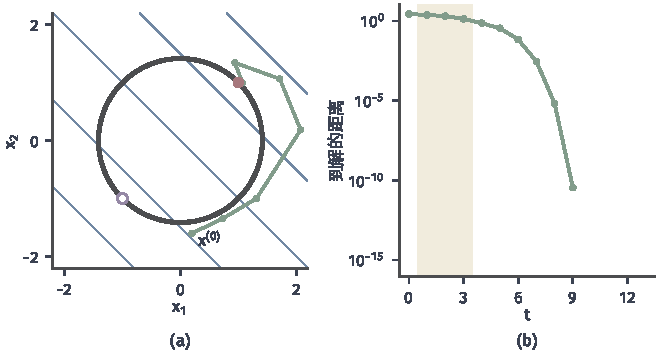
\includegraphics[width=112mm]{figures/05-optimization/06-constrained-optimization/matplotlib/sqp-global-local/figure.pdf}
 \caption{问题~\eqref{eq:sqp-circle}从$(0.2,-1.6)^\top$、$\nu^{(0)}=1$出发的回溯SQP，$\rho=1$，约化曲率不足$0.5$时移位。(a)~路径（绿）绕过圆的右侧到达解（红点），紫色空心点是圆上目标的最大点。(b)~到解的距离，黄色带是步长小于$1$的轮次，此后全步长二次收敛。}
 \label{fig:sqp-global-local}
\end{BookInlineFigure}

运行分成两个阶段。前四轮步长依次是$1,0.25,0.5,0.5$，其中第二到第五轮的约化曲率不足，加了移位，这是接受规则和曲率修正在起作用。之后步长一直是$1$，到解的距离依次为$0.347$、$0.0686$、$0.00289$、$6.7\times10^{-6}$、$3.5\times10^{-11}$，进入Newton的快速段。

\paragraph{停止准则}
“QP解完了”不是结束的标志，判断要回到原问题的KKT残差上。给定容差$\varepsilon_{\mathrm{p}},\varepsilon_{\mathrm{d}},\varepsilon_{\mathrm{c}}>0$，同时检查原始可行、Lagrange驻定和互补三项：
\begin{equation}
 \begin{gathered}
 \lVert\bm{h}(\bm{x})\rVert_\infty\leq\varepsilon_{\mathrm{p}},\qquad\lVert[\bm{g}(\bm{x})]_+\rVert_\infty\leq\varepsilon_{\mathrm{p}},\\
 \lVert\nabla f(\bm{x})+\bm{A}^\top\bm{\nu}+\bm{G}^\top\bm{\lambda}\rVert_\infty\leq\varepsilon_{\mathrm{d}},\\
 \bm{\lambda}\geq\bm{0},\qquad\max_i\lvert\lambda_ig_i(\bm{x})\rvert\leq\varepsilon_{\mathrm{c}}.
 \end{gathered}
 \label{eq:sqp-stopping}
\end{equation}
三项的单位不同，实际中要按目标与约束的尺度归一化。步长很小不能作为收敛的证据，那可能只是回溯失败。

\paragraph{一轮的成本}
表~\ref{tab:sqp-cost}按$n$个变量、$p+m$条约束的稠密情形列出一轮的主要开销。其中QP的迭代次数$k$在热启动的后期常常是$1$或很小的数，而在早期、活动集变动频繁时可能很大。

\begin{BookInlineTable}
 \centering
 \begin{tabular}{ll}
  \toprule
  项目 & 开销\\
  \midrule
  一阶导数 & $\nabla f$与$\bm{A},\bm{G}$各一次\\
  精确曲率 & $m+p+1$个Hessian或Hessian向量积\\
  拟Newton更新 & 约$O(n^2)$\\
  KKT分解（等式） & 约$O((n+p)^3)$，稀疏时远小于此\\
  工作集迭代 & $k$次，每次低秩修正约$O(n^2)$\\
  步的接受 & 每次试探$f$和约束各一次\\
  二阶修正 & 约束一次，再加一次回代\\
  恢复阶段 & 额外的模型构造与子问题求解\\
  \bottomrule
 \end{tabular}
 \caption{SQP一轮的主要开销。}
 \label{tab:sqp-cost}
\end{BookInlineTable}

和第~\ref{chap:penalty-multiplier-methods}章的方法相比，SQP每轮贵得多，一轮要解一个QP，但轮数通常很少，适合函数求值昂贵、约束数目不太大的问题。约束和变量都很多、活动集又难以确定时，分解和工作集迭代的开销变大，第~\ref{chap:nonlinear-interior-point}章的内点法每轮结构更固定，往往更合适。

\section{本章小结}
\label{sec:sqp-summary}

本章从圆周上的小问题出发，回答了章首提出的几个问题。SQP在当前点把目标近似到二阶、把约束近似到一阶，得到一个局部QP。目标的线性项来自$\nabla f$，曲率却要取Lagrange函数的Hessian，因为约束的弯曲只有通过乘子才折算得进模型。所以算法同时维护原始变量和乘子。

只含等式时，局部QP归结为一个KKT线性系统，可以整体分解，也可以分成法向段和零空间内的切向段。行满秩和约化Hessian正定保证解是模型的最小点。取精确Lagrange Hessian时，这个系统正是原问题KKT方程的Newton步。

含不等式时要决定哪些约束算数。有效集法维护工作集，步非零时用比值检验防止越界，步为零时用乘子的符号决定释放哪条约束。有效集法只是QP的一种解法，并不是SQP的一部分，QP也可以用内点法等方法求解。工作集属于当前的线性化QP，只有在约束资格、二阶充分条件和严格互补下，靠近解时才与原问题的活动集一致。

曲率方面，KKT矩阵可逆、约化Hessian正定、$\bm{B}$在全空间正定是三件不同的事。负曲率可以用移位、约化曲率修正或信赖域处理，它们分别改变模型或步长范围。拟Newton近似用同一组乘子下的Lagrange梯度差作割线，用阻尼保持正定，超线性收敛还需要沿步方向的切向曲率逐渐准确。

模型的步要放回原问题检验。罚函数把目标和违反量压成一个数，权重必须超过乘子，又不宜过大；过滤器并排比较两个指标，靠裕量、切换规则和恢复阶段才成为完整的机制。线性化约束无解时用弹性子问题或恢复阶段修复子问题，好步被弯曲约束的二阶违规挡住时用二阶修正修复候选步。恢复失败也不能证明原问题不可行。

最后要分清两类结论。解附近的快速收敛依赖约束资格、二阶充分条件、活动集的识别和全步长的接受；远离解时的可靠进展依赖接受规则和一致有界的曲率。两者条件不同，结论也不同，后者只给出KKT点，并不给出全局最优。全程都要分别检查QP的可行性与原非线性约束的可行性，前者只是后者在切平面上的影子。


\chapter{内点法}
\label{chap:nonlinear-interior-point}

第~\ref{chap:lp-interior-point}章解线性规划时，从可行域内部沿中心路径走向最优解。那里的约束只是$x_i\geq0$，迭代点离每面墙有多远，看坐标就知道。现在换一个问题：在抛物线$x_2\geq x_1^2$与直线$x_2\leq4$围成的区域里，求离点$(3,0)$最近的点。墙是弯的，走一步之后，点离墙有多远要重新计算约束函数才知道。

路径跟踪的骨架可以保留：在边界上立起障碍，放宽互补条件，用Newton法沿参数曲线前进。需要重新回答的问题集中在四处。约束的曲率会进入线性方程组，Newton步可能不再是下降方向。严格内点不再一眼可见，乘子的符号也要专门维护。一个残差很小的点，未必满足原问题的最优性条件。更根本的是，线性规划有多项式时间的保证，一般光滑约束问题没有。

本章只讲这些新增的内容，线性规划里已经讲过的路径跟踪细节直接引用。第一节构造一般约束的障碍子问题，研究路径的存在性和间隙。第二节把松弛变量和乘子纳入同一组方程，推导Newton方向，并讨论步长的接受。第三节回答起点从哪里来、什么时候可以停。第四节把障碍换成二阶锥和半正定锥的形式。第五节说明哪些结论是全局证书，哪些只是局部结果，并计算每一轮的代价。

\section{障碍问题}
\label{sec:nlipm-barrier}

约束是一般的光滑函数时，怎样把“不许越界”写进目标，又让解最终能落到边界上？做法是求解一族带参数的内点子问题，再逐步减小参数。

\paragraph{问题与贯穿例}
本章讨论光滑约束问题
\begin{equation}
 \min_{\bm{x}\in\mathbb{R}^n}\ f(\bm{x})\quad\text{s.t.}\quad g_i(\bm{x})\leq0\ (i=1,\ldots,m),\quad h_j(\bm{x})=0\ (j=1,\ldots,p),
 \label{eq:nlipm-problem}
\end{equation}
其中$f$、$g_i$、$h_j$二阶连续可微。把约束值排成向量$\bm{g}(\bm{x})$、$\bm{h}(\bm{x})$，把它们的梯度按行排成两个Jacobian矩阵：
\begin{equation}
 \bm{J}(\bm{x})=\begin{bmatrix}\nabla g_1(\bm{x})^\top\\\vdots\\\nabla g_m(\bm{x})^\top\end{bmatrix}\in\mathbb{R}^{m\times n},\qquad
 \bm{A}(\bm{x})=\begin{bmatrix}\nabla h_1(\bm{x})^\top\\\vdots\\\nabla h_p(\bm{x})^\top\end{bmatrix}\in\mathbb{R}^{p\times n}.
 \label{eq:nlipm-jacobians}
\end{equation}
本章的$\bm{g}$始终表示约束值，不表示目标的梯度；目标梯度写成$\nabla f$。

全章贯穿下面这个二维例子：
\begin{equation}
 \begin{aligned}
 \min_{\bm{x}}\quad&f(\bm{x})=\tfrac12\bigl((x_1-3)^2+x_2^2\bigr)\\
 \text{s.t.}\quad&g_1(\bm{x})=x_1^2-x_2\leq0,\\
 &g_2(\bm{x})=x_2-4\leq0.
 \end{aligned}
 \label{eq:nlipm-running}
\end{equation}
可行集是抛物线之上、直线$x_2=4$之下的区域，目标是到点$\bm{c}=(3,0)^\top$的距离平方的一半。$g_1$是弯的约束，$g_2$是线性约束。

第~\ref{chap:constrained-optimality}章的KKT条件用到Lagrange函数
\begin{equation}
 \mathcal{L}(\bm{x},\bm{\lambda},\bm{\nu})=f(\bm{x})+\bm{\lambda}^\top\bm{g}(\bm{x})+\bm{\nu}^\top\bm{h}(\bm{x}).
 \label{eq:nlipm-lagrangian}
\end{equation}
条件是说：可行点$\bm{x}^\star$处存在乘子$\bm{\lambda}^\star\geq\bm{0}$和$\bm{\nu}^\star$，使$\mathcal{L}$对$\bm{x}$的梯度为零，并且$\lambda_i^\star g_i(\bm{x}^\star)=0$。

例~\eqref{eq:nlipm-running}中取$\bm{x}^\star=(1,1)^\top$，这时两个约束值和三个梯度是
\[
 g_1=0,\quad g_2=-3,\quad\nabla f=\begin{bmatrix}-2\\1\end{bmatrix},\quad\nabla g_1=\begin{bmatrix}2\\-1\end{bmatrix},\quad\nabla g_2=\begin{bmatrix}0\\1\end{bmatrix}.
\]
于是$\bm{\lambda}^\star=(1,0)^\top$满足全部KKT条件，最优值$f^\star=5/2$。问题是凸的，$\bm{x}^\star$就是全局解。图~\ref{fig:nlipm-running}画出了这一几何关系。

\begin{BookInlineFigure}
  \centering
  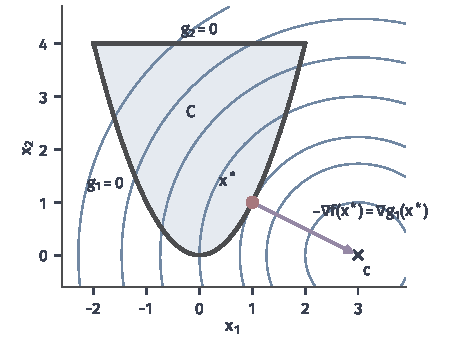
\includegraphics[width=76mm]{figures/05-optimization/06-constrained-optimization/matplotlib/nlipm-running/figure.pdf}
  \caption{贯穿例~\eqref{eq:nlipm-running}。浅蓝区域是可行集$\bm{C}$，深灰粗线是两段边界，蓝线是目标的等值线（以黑叉$\bm{c}=(3,0)$为圆心的圆），红点是最优解$\bm{x}^\star=(1,1)$。紫色箭头同时是$-\nabla f(\bm{x}^\star)$和$\nabla g_1(\bm{x}^\star)$，两者相等对应乘子$\lambda_1^\star=1$；直线边界不活动，乘子为零。}
  \label{fig:nlipm-running}
\end{BookInlineFigure}

\paragraph{内部只对不等式而言}
障碍只能加给不等式，因为只有不等式才有“里面”。记严格可行点的集合为
\begin{equation}
 \bm{C}^{\circ}=\bigl\{\bm{x}:g_i(\bm{x})<0\ (i=1,\ldots,m),\ \bm{h}(\bm{x})=\bm{0}\bigr\}.
 \label{eq:nlipm-strict-set}
\end{equation}
等式约束的可行点构成一张薄片，薄片上没有“离边界远一点”的余地。把$h=0$拆成$h\leq0$和$-h\leq0$也行不通，这两条不等式不可能同时严格成立，拆完之后$\bm{C}^{\circ}$是空集。所以等式约束继续显式保留，加上障碍之后的问题仍然是约束问题，而不是无约束问题。

\subsection{对数障碍}
\label{sec:nlipm-log-barrier}

第~\ref{chap:lp-interior-point}章对$x_i\geq0$用的障碍是$-\log x_i$。约束$x_i\geq0$也可以写成$g_i(\bm{x})=-x_i\leq0$，于是$-\log x_i=-\log(-g_i(\bm{x}))$。这个写法可以直接推广到任何$g_i$。

\begin{definition}[对数障碍函数]
\label{def:nlipm-barrier}
设$\bm{C}^{\circ}$非空。对$\mu>0$，$\bm{g}(\bm{x})<\bm{0}$的点上定义
\begin{equation}
 \phi(\bm{x})=-\sum_{i=1}^m\log\bigl(-g_i(\bm{x})\bigr),\qquad
 B_\mu(\bm{x})=f(\bm{x})+\mu\,\phi(\bm{x}).
 \label{eq:nlipm-barrier-function}
\end{equation}
相应的\term{障碍子问题}（barrier subproblem）是
\begin{equation}
 \min_{\bm{x}}\ B_\mu(\bm{x})\quad\text{s.t.}\quad\bm{h}(\bm{x})=\bm{0},\quad\bm{g}(\bm{x})<\bm{0}.
 \label{eq:nlipm-barrier-problem}
\end{equation}
\end{definition}

点靠近某条约束的边界时，$-g_i\downarrow0$，$\phi\to+\infty$。边界像一堵墙，迭代点靠函数值的上升留在内部。例~\eqref{eq:nlipm-running}的障碍目标是
\[
 B_\mu(\bm{x})=\tfrac12\bigl((x_1-3)^2+x_2^2\bigr)-\mu\log(x_2-x_1^2)-\mu\log(4-x_2).
\]
图~\ref{fig:nlipm-barrier-bowls}画出两个参数下的等值线。参数较大时碗底靠近区域中央，参数较小时等值线贴向边界，碗底被目标拉向$\bm{x}^\star$。

\begin{BookInlineFigure}
  \centering
  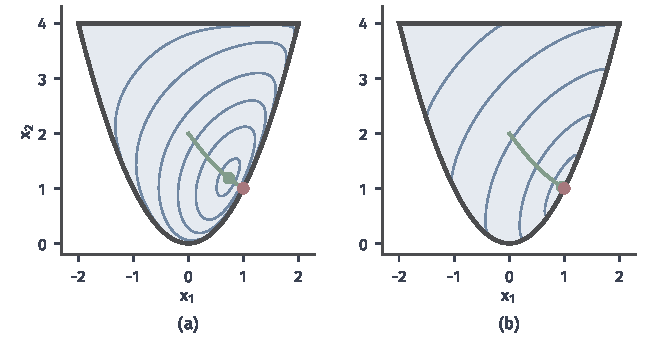
\includegraphics[width=112mm]{figures/05-optimization/06-constrained-optimization/matplotlib/nlipm-barrier-bowls/figure.pdf}
  \caption{贯穿例的障碍目标$B_\mu$在可行集内的等值线（蓝线）。(a)$\mu=1$；(b)$\mu=0.1$。绿线是各参数下碗底连成的曲线，绿点是当前参数的碗底，红点是$\bm{x}^\star$。}
  \label{fig:nlipm-barrier-bowls}
\end{BookInlineFigure}

\paragraph{约束的梯度和Hessian怎样进入}
求导只需要复合函数法则。对一元函数$\psi(u)=-\log(-u)$（$u<0$），有
\[
 \psi'(u)=\frac{1}{-u},\qquad\psi''(u)=\frac{1}{u^2}.
\]
把$u=g_i(\bm{x})$代入，并对$i$求和，得到障碍函数的梯度和Hessian：
\begin{align}
 \nabla\phi(\bm{x})&=\sum_{i=1}^m\frac{1}{-g_i(\bm{x})}\,\nabla g_i(\bm{x}),
 \label{eq:nlipm-barrier-grad}\\
 \nabla^2\phi(\bm{x})&=\sum_{i=1}^m\frac{\nabla g_i(\bm{x})\nabla g_i(\bm{x})^\top}{g_i(\bm{x})^2}
 +\sum_{i=1}^m\frac{\nabla^2g_i(\bm{x})}{-g_i(\bm{x})}.
 \label{eq:nlipm-barrier-hess}
\end{align}

式~\eqref{eq:nlipm-barrier-hess}的两项作用不同。第一项是秩一矩阵之和，只在约束的法向产生曲率，点越靠近边界越大，这就是“墙”的刚度。第二项把约束本身的弯曲带进来，线性规划中$\nabla^2g_i=\bm{0}$，这一项不存在，所以它正是本章新增的内容。

在贯穿例的点$\bm{x}=(1,2)^\top$上算一次。约束值与约束梯度是
\[
 g_1=-1,\quad g_2=-2,\quad\nabla g_1=\begin{bmatrix}2\\-1\end{bmatrix},\quad\nabla g_2=\begin{bmatrix}0\\1\end{bmatrix},\quad\nabla^2g_1=\begin{bmatrix}2&0\\0&0\end{bmatrix}.
\]
代入式~\eqref{eq:nlipm-barrier-grad}，得到
\[
 \nabla\phi=1\cdot\begin{bmatrix}2\\-1\end{bmatrix}+\frac12\begin{bmatrix}0\\1\end{bmatrix}=\begin{bmatrix}2\\-1/2\end{bmatrix}.
\]
代入式~\eqref{eq:nlipm-barrier-hess}，三块矩阵相加：
\[
 \nabla^2\phi=\begin{bmatrix}4&-2\\-2&1\end{bmatrix}+\begin{bmatrix}0&0\\0&1/4\end{bmatrix}+\begin{bmatrix}2&0\\0&0\end{bmatrix}=\begin{bmatrix}6&-2\\-2&5/4\end{bmatrix}.
\]
最后一块$\operatorname{diag}(2,0)$来自抛物线的弯曲，如果把$g_1$换成切线，它就消失了。

\paragraph{一维边界例子：内点步受到的限制}
Newton法用二次模型近似$B_\mu$，而障碍函数在边界附近根本不像二次函数。看最简单的弯约束：
\[
 \min_x\ x\quad\text{s.t.}\quad x^2-1\leq0.
\]
解是$x^\star=-1$。障碍目标$B_\mu(x)=x-\mu\log(1-x^2)$的导数是
\[
 B_\mu'(x)=1+\frac{2\mu x}{1-x^2},\qquad B_\mu''(x)=\frac{2\mu(1+x^2)}{(1-x^2)^2}.
\]
令$B_\mu'(x)=0$，得到$1-x^2+2\mu x=0$。在$(-1,1)$内的根是
\begin{equation}
 x(\mu)=\mu-\sqrt{\mu^2+1}.
 \label{eq:nlipm-1d-center}
\end{equation}
取几个能算成分数的值：$\mu=3/4$时$x=-1/2$，$\mu=5/12$时$x=-2/3$。

现在站在$\mu=3/4$的碗底$x=-1/2$，把参数减小到$\mu^+$，走一个Newton步。在这一点上
\[
 \frac{2x}{1-x^2}=-\frac43,\qquad\frac{2(1+x^2)}{(1-x^2)^2}=\frac{40}{9}.
\]
于是Newton步是
\[
 d=-\frac{1-\tfrac43\mu^+}{\tfrac{40}{9}\mu^+}=-\frac{9-12\mu^+}{40\mu^+}.
\]

$\mu^+=5/12$时$d=-6/25$，新点$-0.74$仍在区间内，离新的碗底$-2/3$不远。$\mu^+=0.05$时$d=-4.2$，新点是$-4.7$，已经远在可行域之外，如图~\ref{fig:nlipm-barrier-1d}(b)所示。要让单位步留在区间内，需要$d>-1/2$，解这个不等式，得到
\[
 \mu^+>\frac{9}{32}.
\]
也就是说，这一点上参数最多缩小到原来的$3/8$。参数一次减得太多，碗底搬走了，二次模型却还停留在旧的位置。

\begin{BookInlineFigure}
  \centering
  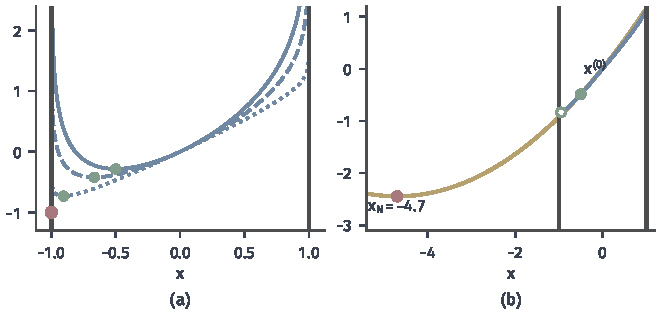
\includegraphics[width=112mm]{figures/05-optimization/06-constrained-optimization/matplotlib/nlipm-barrier-1d/figure.pdf}
  \caption{一维边界例子$\min x$，$x^2\leq1$。(a)蓝线是$B_\mu$，实线、虚线、点线分别对应$\mu=3/4$、$5/12$、$0.1$，绿点是碗底，红点是解$x^\star=-1$，深灰粗线是边界$x=\pm1$。(b)参数减到$\mu^+=0.05$，蓝线是$B_{\mu^+}$，只在区间内有定义；黄线是在绿点$x^{(0)}=-1/2$处的二次模型，其极小点（红点）落在$-4.7$；空心绿点是新的碗底。}
  \label{fig:nlipm-barrier-1d}
\end{BookInlineFigure}

\paragraph{新的曲率与凸性}
约束的弯曲方向决定第二项的符号。$g_i$凸时$\nabla^2g_i\succeq\bm{0}$，第二项半正定，障碍函数保持凸性。

\begin{lemma}[凸约束的障碍是凸函数]
\label{lem:nlipm-barrier-convex}
设每个$g_i$在开集上凸且二阶连续可微，则$\phi$在集合$\{\bm{x}:\bm{g}(\bm{x})<\bm{0}\}$的每个凸子集上是凸函数。
\end{lemma}

\begin{proof}
式~\eqref{eq:nlipm-barrier-hess}中，第一项是半正定矩阵的非负组合。第二项中$-g_i>0$，$\nabla^2g_i\succeq\bm{0}$，也是半正定矩阵的非负组合。所以$\nabla^2\phi\succeq\bm{0}$。
\end{proof}

$g_i$非凸时，这个结论没有理由成立，用了对数也不会自动得到凸子问题。看单位圆盘的外部，约束是$g(\bm{x})=1-\lVert\bm{x}\rVert_2^2\leq0$。这时$\nabla^2g=-2\bm{I}$，式~\eqref{eq:nlipm-barrier-hess}给出
\[
 \nabla^2\phi(\bm{x})=\frac{4\bm{x}\bm{x}^\top}{(\lVert\bm{x}\rVert_2^2-1)^2}-\frac{2\bm{I}}{\lVert\bm{x}\rVert_2^2-1}.
\]
沿与$\bm{x}$垂直的切向，第一项为零，第二项是负的，曲率等于$-2/(\lVert\bm{x}\rVert_2^2-1)$，离边界越近越负。

图~\ref{fig:nlipm-nonconvex-barrier}取目标$x_2^2+0.12(x_1-1/2)^2$，并取$\mu=0.1$。障碍目标有两个彼此隔开的局部极小点，分别在圆盘的右侧和左侧。图(b)沿点$(1.5,0)$处的切向对比两种约束：外部约束的障碍在这一点是山顶形状，圆盘内部约束的障碍则是碗。

\begin{BookInlineFigure}
  \centering
  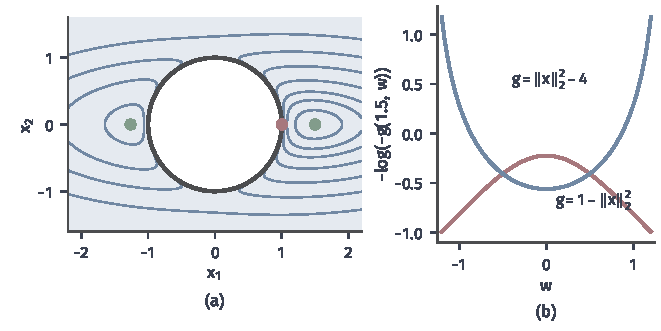
\includegraphics[width=112mm]{figures/05-optimization/06-constrained-optimization/matplotlib/nlipm-nonconvex-barrier/figure.pdf}
  \caption{非凸约束的障碍。(a)可行集是单位圆盘的外部（浅蓝），蓝线是$B_{0.1}$的等值线，两个绿点是障碍目标的局部极小点，红点是原问题的全局解$(1,0)$。(b)沿$x_1=1.5$的切向，红线是外部约束$g=1-\lVert\bm{x}\rVert_2^2$的障碍，在$w=0$处曲率为负；蓝线是圆盘内部约束$g=\lVert\bm{x}\rVert_2^2-4$的障碍，曲率为正。}
  \label{fig:nlipm-nonconvex-barrier}
\end{BookInlineFigure}

\subsection{参数与路径}
\label{sec:nlipm-parameter-path}

固定一个$\mu$，子问题~\eqref{eq:nlipm-barrier-problem}有没有解？解随$\mu$怎样变？这一小节先用驻定条件把子问题和KKT条件联系起来，再分凸问题和非凸问题回答这两个问题。

\paragraph{驻定条件就是扰动的互补}
子问题~\eqref{eq:nlipm-barrier-problem}的一阶条件是：存在$\bm{\nu}$，使
\[
 \nabla B_\mu(\bm{x})+\bm{A}(\bm{x})^\top\bm{\nu}=\bm{0}.
\]
把式~\eqref{eq:nlipm-barrier-grad}代入，得到
\[
 \nabla f(\bm{x})+\sum_{i=1}^m\frac{\mu}{-g_i(\bm{x})}\nabla g_i(\bm{x})+\bm{A}(\bm{x})^\top\bm{\nu}=\bm{0}.
\]

求和中的系数都是正数，并且正好处在KKT条件中乘子的位置。令$\lambda_i=\mu/(-g_i(\bm{x}))$，条件变成
\begin{equation}
 \begin{gathered}
 \nabla f(\bm{x})+\bm{J}(\bm{x})^\top\bm{\lambda}+\bm{A}(\bm{x})^\top\bm{\nu}=\bm{0},\qquad\bm{h}(\bm{x})=\bm{0},\\
 \lambda_i\bigl(-g_i(\bm{x})\bigr)=\mu\ (i=1,\ldots,m),\qquad\bm{g}(\bm{x})<\bm{0},\quad\bm{\lambda}>\bm{0}.
 \end{gathered}
 \label{eq:nlipm-perturbed-kkt}
\end{equation}
与KKT条件逐项比较，只有互补一处不同：$\lambda_ig_i=0$换成了$\lambda_i(-g_i)=\mu$。这和第~\ref{chap:lp-interior-point}章的$x_is_i=\mu$是同一件事。乘子不是另外猜出来的，它就是障碍项在该约束上施加的推力，$\lambda_i=\mu/(-g_i)$离墙越近越大。

\paragraph{子问题的解何时存在}
碗底的存在要靠水平集被围住。下面的定理说明，可行集有界时墙就足够了。

\begin{theorem}[障碍子问题的解]
\label{thm:nlipm-barrier-exists}
设$f$、$g_i$、$h_j$连续，可行集$\bm{C}$有界，$\bm{C}^{\circ}$非空，$\mu>0$。则$B_\mu$在$\bm{C}^{\circ}$上取到最小值。

再设$f$、$g_i$凸且二阶连续可微，$\bm{h}(\bm{x})=\bm{A}\bm{x}-\bm{b}$，$\bm{A}$满行秩，并且不存在非零的$\bm{d}$同时满足
\begin{equation}
 \bm{A}\bm{d}=\bm{0},\quad\bm{d}^\top\nabla^2f\bm{d}=0,\quad\nabla g_i^\top\bm{d}=0,\quad\bm{d}^\top\nabla^2g_i\bm{d}=0\ (\forall i)
 \label{eq:nlipm-unique-condition}
\end{equation}
（各导数在$\bm{C}^{\circ}$的任一点取值）。则最小点$\bm{x}(\mu)$唯一，方程组~\eqref{eq:nlipm-perturbed-kkt}有唯一解$(\bm{x}(\mu),\bm{\lambda}(\mu),\bm{\nu}(\mu))$。
\end{theorem}

\begin{proof}
先证存在。$\bm{C}$是有界闭集，$f$和每个$-g_i$在其上连续，所以存在常数$F$和$G>1$，使$\lvert f\rvert\leq F$，$-g_i\leq G$。

取$\bm{x}^{(0)}\in\bm{C}^{\circ}$，考虑下水平集
\[
 \bigl\{\bm{x}\in\bm{C}^{\circ}:B_\mu(\bm{x})\leq B_\mu(\bm{x}^{(0)})\bigr\}.
\]
对其中的点和任一下标$i$，把其余各项移到右边，得到
\[
 -\mu\log\bigl(-g_i(\bm{x})\bigr)\leq B_\mu(\bm{x}^{(0)})+F+\mu(m-1)\log G.
\]
右端是常数，所以存在$\epsilon>0$，使$-g_i(\bm{x})\geq\epsilon$。这说明水平集是$\bm{C}$的闭子集，从而是紧集，连续函数$B_\mu$在其上取到最小值。

再证唯一。由引理~\ref{lem:nlipm-barrier-convex}，$B_\mu$凸。对满足$\bm{A}\bm{d}=\bm{0}$的非零$\bm{d}$，式~\eqref{eq:nlipm-barrier-hess}给出
\[
 \bm{d}^\top\nabla^2B_\mu\bm{d}=\bm{d}^\top\nabla^2f\bm{d}+\mu\sum_{i=1}^m\Bigl(\frac{(\nabla g_i^\top\bm{d})^2}{g_i^2}+\frac{\bm{d}^\top\nabla^2g_i\bm{d}}{-g_i}\Bigr).
\]
右端各项非负，由条件~\eqref{eq:nlipm-unique-condition}，它们不全为零，所以$B_\mu$在仿射集上严格凸，最小点唯一。

最后看方程组。最小点处梯度与$\bm{A}$的零空间正交，所以存在$\bm{\nu}$使驻定条件成立，$\bm{A}$满行秩使$\bm{\nu}$唯一，$\bm{\lambda}$由$\lambda_i=\mu/(-g_i)$确定。反过来，方程组的解满足凸函数$B_\mu$在仿射集上的一阶条件，因此就是最小点。
\end{proof}

存在性的第一部分没有用到凸性，它只用到有界和连续。可行集无界时，这个结论可能失败。问题$\min 0$、$-x\leq0$的最优解集是$[0,\infty)$，障碍目标$-\mu\log x$在$x\to\infty$时趋于$-\infty$，没有最小点。条件~\eqref{eq:nlipm-unique-condition}在贯穿例中成立，因为$\nabla^2f=\bm{I}$，第二项已经排除了所有非零方向。

\paragraph{路径}
定理的条件成立时，$\mu$取遍$(0,\infty)$，解连成一条曲线，沿用第~\ref{chap:lp-interior-point}章的名字，称为中心路径。图~\ref{fig:nlipm-central-path}画出贯穿例的路径。当$\mu\to\infty$时，目标的作用可以忽略，点趋于$\phi$的最小点，即解析中心。贯穿例的解析中心可以直接求：对称性给出$x_1=0$，再由$-1/x_2+1/(4-x_2)=0$得到$x_2=2$。

\begin{BookInlineFigure}
  \centering
  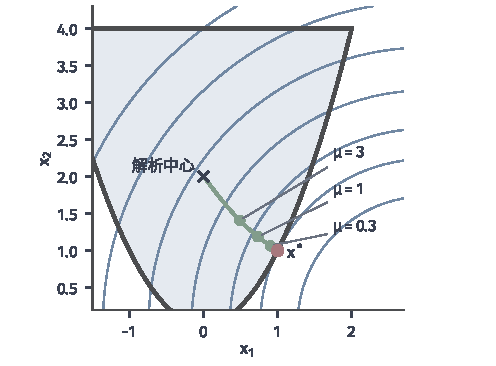
\includegraphics[width=84mm]{figures/05-optimization/06-constrained-optimization/matplotlib/nlipm-central-path/figure.pdf}
  \caption{贯穿例的中心路径（绿线）。黑叉是解析中心$(0,2)$，绿点是$\mu=3$、$1$、$0.3$对应的中心点，红点是$\bm{x}^\star=(1,1)$，蓝线是目标的等值线。路径是弯的，因为不活动的直线约束的影响在逐渐消失。}
  \label{fig:nlipm-central-path}
\end{BookInlineFigure}

这个例子的路径可以化成一元方程。由方程组~\eqref{eq:nlipm-perturbed-kkt}的第一行，$\lambda_1=(3-x_1)/(2x_1)$。取$\mu=1$，用Newton法解出的中心点和乘子是
\[
 \bm{x}(1)\approx(0.7343,1.1873)^\top,\qquad\bm{\lambda}(1)\approx(1.5428,0.3555)^\top.
\]
可以核对互补：$\lambda_1(x_2-x_1^2)=1.5428\times0.6481\approx1$，$\lambda_2(4-x_2)=0.3555\times2.8127\approx1$。

图~\ref{fig:nlipm-path-multipliers}(a)显示乘子沿路径的走向。活动约束的乘子$\lambda_1(\mu)$趋于$\lambda_1^\star=1$，不活动约束的乘子$\lambda_2(\mu)$按$\mu/3$的量级趋于零，这里的$3$就是直线约束在解处的松弛。乘子估计本身就在告诉我们哪条约束活动，这一点不需要事先猜测。

\paragraph{凸问题的间隙}
第~\ref{chap:lp-interior-point}章中，沿路径的对偶间隙恰好是$n\mu$。一般凸问题也有同样的结果，只是$n$要换成不等式的条数$m$。

\begin{theorem}[路径上的间隙]
\label{thm:nlipm-gap}
设$f$、$g_i$凸且可微，$\bm{h}(\bm{x})=\bm{A}\bm{x}-\bm{b}$，$(\bm{x},\bm{\lambda},\bm{\nu})$满足方程组~\eqref{eq:nlipm-perturbed-kkt}，$f^\star$是问题~\eqref{eq:nlipm-problem}在可行集上的下确界。则
\begin{equation}
 f(\bm{x})-m\mu\leq f^\star\leq f(\bm{x}).
 \label{eq:nlipm-gap}
\end{equation}
\end{theorem}

\begin{proof}
右边的不等式成立是因为$\bm{x}$可行。对左边，任取可行点$\bm{x}'$。因为$\bm{\lambda}>\bm{0}$、$\bm{g}(\bm{x}')\leq\bm{0}$、$\bm{h}(\bm{x}')=\bm{0}$，有
\[
 f(\bm{x}')\geq f(\bm{x}')+\bm{\lambda}^\top\bm{g}(\bm{x}')+\bm{\nu}^\top\bm{h}(\bm{x}')=\mathcal{L}(\bm{x}',\bm{\lambda},\bm{\nu}).
\]

$\mathcal{L}(\cdot,\bm{\lambda},\bm{\nu})$是凸函数，并且在$\bm{x}$处梯度为零，所以$\bm{x}$是它的全局最小点：
\[
 \mathcal{L}(\bm{x}',\bm{\lambda},\bm{\nu})\geq\mathcal{L}(\bm{x},\bm{\lambda},\bm{\nu}).
\]

再用$\bm{h}(\bm{x})=\bm{0}$和$\lambda_ig_i(\bm{x})=-\mu$，得到
\[
 \mathcal{L}(\bm{x},\bm{\lambda},\bm{\nu})=f(\bm{x})+\sum_{i=1}^m\lambda_ig_i(\bm{x})=f(\bm{x})-m\mu.
\]
三式相连，对$\bm{x}'$取下确界即得。
\end{proof}

式~\eqref{eq:nlipm-gap}的左端是一个对偶值，它由当前点直接算出，不需要知道$\bm{x}^\star$。要保证目标误差不超过$\varepsilon$，走到$\mu\leq\varepsilon/m$就够了。

这个界数的是全部$m$条约束，实际误差往往更小。图~\ref{fig:nlipm-path-multipliers}(b)中，贯穿例的$f(\bm{x}(\mu))-f^\star$在$\mu$小时约等于$\mu$，而不是$2\mu$。原因是不活动的约束虽然也贡献了$\lambda_2s_2=\mu$，它却只是把对偶值往下拉，并不代表目标还有这么多可以下降。

\begin{BookInlineFigure}
  \centering
  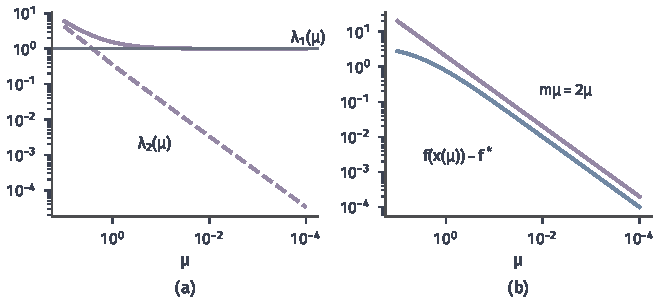
\includegraphics[width=112mm]{figures/05-optimization/06-constrained-optimization/matplotlib/nlipm-path-multipliers/figure.pdf}
  \caption{贯穿例沿中心路径的量，横轴是$\mu$，向右减小。(a)紫色实线是$\lambda_1(\mu)$，趋于$\lambda_1^\star=1$（灰线）；紫色虚线是$\lambda_2(\mu)$，随$\mu$线性趋于零。(b)紫线是定理的界$m\mu=2\mu$，蓝线是实际误差$f(\bm{x}(\mu))-f^\star$。}
  \label{fig:nlipm-path-multipliers}
\end{BookInlineFigure}

\paragraph{固定参数时解多准，参数降多快}
这样就得到\term{障碍法}（barrier method）：外层维护参数$\mu$，内层从上一个点出发，用第~\ref{chap:second-order-methods}章的阻尼Newton法解子问题~\eqref{eq:nlipm-barrier-problem}，解到Newton减量足够小，再令$\mu\leftarrow\tau\mu$，其中$\tau\in(0,1)$。回溯时要多加一条规则，试探点若使某个$g_i\geq0$，直接拒绝。

以贯穿例从$\bm{x}^{(0)}=(1,2)^\top$、$\mu=1$开始。前面已经算出$\nabla\phi$和$\nabla^2\phi$，把目标的导数加上，得到
\[
 \nabla B_1=\begin{bmatrix}0\\3/2\end{bmatrix},\qquad\nabla^2B_1=\begin{bmatrix}7&-2\\-2&9/4\end{bmatrix}.
\]
解线性方程组，Newton方向是
\[
 \bm{d}=\Bigl(-\frac{12}{47},\,-\frac{42}{47}\Bigr)^\top\approx(-0.2553,\,-0.8936)^\top.
\]
单位步后的点$(0.7447,1.1064)^\top$仍然严格可行，再走两步就到达$\bm{x}(1)$附近。

外层有两种取舍。$\tau$接近$1$时，上一个点几乎就是新碗底，每轮只需一两个Newton步，但要走很多轮。$\tau$很小时，轮数少，但正如一维例子所示，起步时Newton步很不可靠，每轮要靠回溯慢慢走。

图~\ref{fig:nlipm-update-tradeoff}是贯穿例上的实测，从解析中心出发，要求$m\mu\leq10^{-6}$。$\tau=0.9$时总共要$218$个Newton步，$\tau=0.5$时$38$步，$\tau=0.1$时$32$步，$\tau=0.001$时只要$18$步，单轮最多也不过$6$步。这说明Newton步的总数对$\tau$不敏感，只有$\tau$过于接近$1$时明显吃亏。

这是一个二维小例子上的观察，并且总数随$\tau$并不单调。规模增大时，大幅度减小参数的代价一般会更明显，第~\ref{sec:nlipm-guarantees}节再谈理论上的界。

\begin{BookInlineFigure}
  \centering
  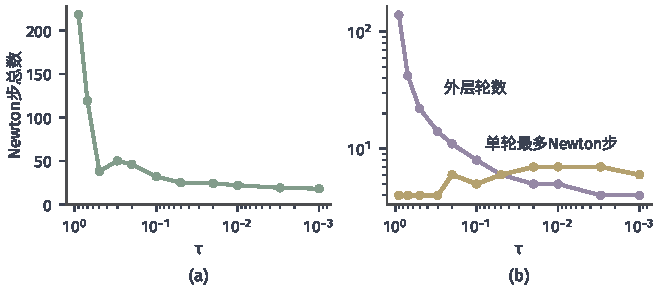
\includegraphics[width=112mm]{figures/05-optimization/06-constrained-optimization/matplotlib/nlipm-update-tradeoff/figure.pdf}
  \caption{贯穿例上障碍法的工作量，$\mu^{(0)}=1$，内层Newton减量阈值$10^{-8}$，横轴是参数缩小倍率$\tau$，向右更激进。(a)Newton步总数。(b)紫线是外层轮数，黄线是单轮最多的Newton步数。}
  \label{fig:nlipm-update-tradeoff}
\end{BookInlineFigure}

\paragraph{非凸问题只能谈局部路径}
没有凸性时，定理~\ref{thm:nlipm-gap}的推理在“$\bm{x}$是$\mathcal{L}$的全局最小点”这一步断掉，方程组~\eqref{eq:nlipm-perturbed-kkt}的解也不必唯一。能保证的是在一个性质好的KKT点附近，有一段路径通向它。

\begin{theorem}[KKT点附近的路径]
\label{thm:nlipm-local-path}
设$f$、$g_i$、$h_j$二阶连续可微，$(\bm{x}^\star,\bm{\lambda}^\star,\bm{\nu}^\star)$是KKT点，并满足三个条件：活动约束梯度与全部等式约束梯度线性无关；严格互补，即活动约束的乘子都为正；在临界方向上有
\begin{equation}
 \bm{d}^\top\nabla_{\bm{x}\bm{x}}^2\mathcal{L}(\bm{x}^\star,\bm{\lambda}^\star,\bm{\nu}^\star)\bm{d}>0,
 \label{eq:nlipm-sosc}
\end{equation}
这里临界方向指满足$\bm{A}\bm{d}=\bm{0}$、对活动约束$\nabla g_i^\top\bm{d}=0$的非零$\bm{d}$。则存在$\bar{\mu}>0$和连续可微的曲线$\mu\mapsto(\bm{x}(\mu),\bm{\lambda}(\mu),\bm{\nu}(\mu))$，在$(0,\bar{\mu})$上满足方程组~\eqref{eq:nlipm-perturbed-kkt}，$\mu\downarrow0$时趋于该KKT点，并且$\bm{x}(\mu)$是子问题~\eqref{eq:nlipm-barrier-problem}的严格局部极小点。
\end{theorem}

\begin{proof}
设$\bm{s}=-\bm{g}$，把方程组写成关于$(\bm{x},\bm{s},\bm{\lambda},\bm{\nu})$的方程$\bm{F}(\cdot)=\mu\bm{e}$，其中$\bm{e}$只在互补方程处为$1$。在$\mu=0$的KKT点处用隐函数定理，只需证明Jacobian矩阵非奇异，也就是下面的齐次方程只有零解：
\[
 \begin{gathered}
 \bm{W}\bm{d}+\bm{J}^\top\bm{d}_\lambda+\bm{A}^\top\bm{d}_\nu=\bm{0},\qquad\bm{A}\bm{d}=\bm{0},\\
 \bm{J}\bm{d}+\bm{d}_s=\bm{0},\qquad\lambda_i^\star d_{s,i}+s_i^\star d_{\lambda,i}=0.
 \end{gathered}
\]
这里$\bm{W}=\nabla^2_{\bm{x}\bm{x}}\mathcal{L}$。

对活动约束，$s_i^\star=0$、$\lambda_i^\star>0$，互补方程给出$d_{s,i}=0$，于是$\nabla g_i^\top\bm{d}=0$。对不活动约束，$\lambda_i^\star=0$、$s_i^\star>0$，互补方程给出$d_{\lambda,i}=0$。

用$\bm{d}^\top$左乘第一个方程，再用$\bm{A}\bm{d}=\bm{0}$，得到
\[
 \bm{d}^\top\bm{W}\bm{d}=-\sum_{i}d_{\lambda,i}\nabla g_i^\top\bm{d}=0.
\]
求和中每一项都为零：活动约束的$\nabla g_i^\top\bm{d}=0$，不活动约束的$d_{\lambda,i}=0$。由条件~\eqref{eq:nlipm-sosc}，$\bm{d}=\bm{0}$。

于是$\bm{d}_s=\bm{0}$，第一个方程只剩活动约束与等式约束的梯度组合等于零，由线性无关性，$\bm{d}_\lambda$、$\bm{d}_\nu$为零。隐函数定理给出连续可微的解曲线。对小的$\mu>0$，活动约束$s_i=\mu/\lambda_i>0$，不活动约束$\lambda_i=\mu/s_i>0$，所以解满足正性要求。

最后证局部极小。把式~\eqref{eq:nlipm-barrier-hess}和$\lambda_i=\mu/s_i$代入$\nabla^2B_\mu$，并计入等式约束的曲率，子问题的Lagrange Hessian是$\bm{W}+\bm{J}^\top\bm{S}^{-1}\bm{\Lambda}\bm{J}$，其中$\bm{S}$、$\bm{\Lambda}$是对角矩阵。假设存在$\mu_k\downarrow0$和单位向量$\bm{d}_k$，满足$\bm{A}\bm{d}_k=\bm{0}$，而二次型非正。则
\[
 \sum_{i}\frac{\lambda_i}{s_i}(\nabla g_i^\top\bm{d}_k)^2\leq-\bm{d}_k^\top\bm{W}\bm{d}_k.
\]
右端有界，而活动约束的$\lambda_i/s_i\to\infty$，所以极限方向$\bar{\bm{d}}$满足$\nabla g_i^\top\bar{\bm{d}}=0$。于是$\bar{\bm{d}}$是临界方向，并且$\bar{\bm{d}}^\top\bm{W}\bar{\bm{d}}\leq0$，与式~\eqref{eq:nlipm-sosc}矛盾。
\end{proof}

定理的三个条件各管一件事。线性无关保证乘子唯一，严格互补保证每条约束在极限时明确属于活动或不活动的一侧，式~\eqref{eq:nlipm-sosc}保证弯曲方向上是极小而不是鞍点。

隐函数定理还给出路径在$\mu=0$处的切线。在贯穿例中，$\bm{W}=\operatorname{diag}(3,1)$，$s_2^\star=3$，把解曲线对$\mu$求导，得到
\[
 \lambda_2'(0)=\frac13,\qquad s_1'(0)=1.
\]
线性化的方程剩下三个未知量$x_1'$、$x_2'$、$\lambda_1'$，解出
\[
 \bm{x}'(0)=\Bigl(-\frac{8}{21},\,\frac{5}{21}\Bigr)^\top,\qquad\lambda_1'(0)=\frac47.
\]
所以$\bm{x}(\mu)\approx(1,1)^\top+\mu(-8/21,5/21)^\top$。取$\mu=0.01$，预测$(0.9962,1.0024)^\top$，数值解是$(0.9962,1.0024)^\top$。目标的一阶变化是$\nabla f^\top\bm{x}'(0)=1$，这正是前面看到的“误差约等于$\mu$”。

\paragraph{路径可以断开，也可能通向较差的解}
定理~\ref{thm:nlipm-local-path}的$\bar{\mu}$可以很小，它不保证路径能一直延伸到大的$\mu$。下面的一维例子说明会发生什么。在$x>0$上取$f'(x)=(x-1)(x-3)(x-4)$，它在$x=1$和$x=4$处有局部极小，$f(4)-f(1)=9/4$，所以$x=1$是全局解。

障碍驻定条件$f'(x)=\mu/x$可以反解成
\[
 \mu=x(x-1)(x-3)(x-4).
\]
要求$\mu>0$，可行的$x$只有$(1,3)$和$(4,\infty)$两段。第一段上$\mu$先增后减，在$x=2$处达到最大值$\mu=4$。图~\ref{fig:nlipm-nonconvex-fold}(b)中，极小点的分支从$x=1$出发，到$\mu=4$时与鞍点分支相撞，两者同时消失，这个点称为\term{折叠点}（fold point）。

$\mu>4$时只剩$x>4$这一支。从大的$\mu$出发沿路径减小参数，走到的是$x=4$，错过了全局解$x=1$。这条路径是连续的，算法并没有失败，只是路径根本不经过全局解。

\begin{BookInlineFigure}
  \centering
  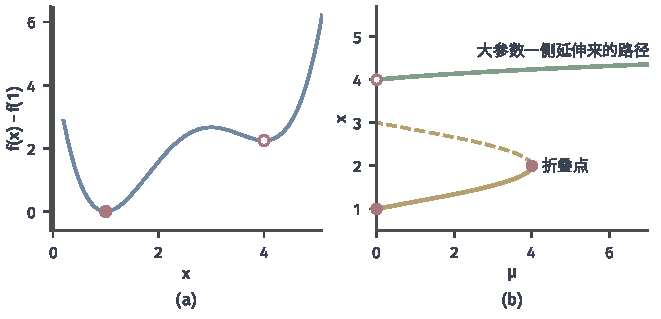
\includegraphics[width=112mm]{figures/05-optimization/06-constrained-optimization/matplotlib/nlipm-nonconvex-fold/figure.pdf}
  \caption{非凸的一维路径，$f'(x)=(x-1)(x-3)(x-4)$，$x>0$。(a)蓝线是目标，红点是全局解$x=1$，空心红点是局部解$x=4$。(b)$(\mu,x)$平面上的驻点集合：绿线是从大参数一侧延伸来的路径；黄线是$(1,3)$上的另一支，实线部分是局部极小点，虚线部分不是，两者在红点（折叠点$(4,2)$）相遇。}
  \label{fig:nlipm-nonconvex-fold}
\end{BookInlineFigure}

\section{原始—对偶内点法}
\label{sec:nlipm-primal-dual}

障碍法有两个不便之处。一维例子已经显示，参数减小之后，从旧碗底出发的Newton步可能完全不可信。另外它要求每个迭代点都严格满足$\bm{g}(\bm{x})<\bm{0}$，弯的约束使这件事代价不小。于是要问：把乘子和松弛都当作独立变量，同时更新，能否绕开这两点，又要付出什么代价？

\subsection{扰动互补方程}
\label{sec:nlipm-perturbed}

方程组~\eqref{eq:nlipm-perturbed-kkt}里，$-g_i$既是约束值，又是互补方程的一个因子。引入\term{松弛变量}（slack variable）$\bm{s}\in\mathbb{R}^m$，把它们分开：
\begin{equation}
 \begin{aligned}
 \nabla f(\bm{x})+\bm{J}(\bm{x})^\top\bm{\lambda}+\bm{A}(\bm{x})^\top\bm{\nu}&=\bm{0},\\
 \bm{h}(\bm{x})&=\bm{0},\\
 \bm{g}(\bm{x})+\bm{s}&=\bm{0},\\
 s_i\lambda_i&=\mu\quad(i=1,\ldots,m),\\
 \bm{s}>\bm{0},\quad\bm{\lambda}&>\bm{0}.
 \end{aligned}
 \label{eq:nlipm-pd-system}
\end{equation}
这里的乘子$\bm{\lambda}$沿用第~\ref{chap:constrained-optimality}章的符号。要留意$\bm{s}$的角色变了：第~\ref{chap:lp-interior-point}章的$\bm{s}$是对偶松弛，这里的$\bm{s}$是原始松弛，对偶一侧的正变量是$\bm{\lambda}$。表~\ref{tab:nlipm-lp-correspondence}列出两章量的对应，取$\bm{g}(\bm{x})=-\bm{x}$就回到线性规划。

\begin{BookInlineTable}
  \centering
  \footnotesize
  \begin{tabular}{@{}lll@{}}
    \toprule
    量 & 线性规划 & 一般约束\\
    \midrule
    原始侧的正变量 & $\bm{x}$ & $\bm{s}=-\bm{g}(\bm{x})$\\
    对偶侧的正变量 & $\bm{s}$ & $\bm{\lambda}$\\
    扰动互补 & $x_is_i=\mu$ & $s_i\lambda_i=\mu$\\
    不等式约束数 & $n$ & $m$\\
    Jacobian & $-\bm{I}$，常数 & $\bm{J}(\bm{x})$，随点变化\\
    等式的Jacobian & $\bm{A}$，常数 & $\bm{A}(\bm{x})$，随点变化\\
    二阶信息 & 无 & Lagrange Hessian\\
    \bottomrule
  \end{tabular}
  \caption{线性规划内点法与一般约束内点法中各量的对应。}
  \label{tab:nlipm-lp-correspondence}
\end{BookInlineTable}

\paragraph{正性和参数各管什么}
方程组~\eqref{eq:nlipm-pd-system}有两类要求，作用不同。$\bm{s},\bm{\lambda}>\bm{0}$是内部性，它不是方程，而是对解的筛选。$\mu>0$是中心性，它要求所有乘积相等，从而把组合选择（哪个因子为零）换成一条光滑的曲线。

去掉正性，方程会多出不该要的解。回到一维例子$\min x$、$x^2-1\leq0$，方程组是
\[
 1+2\lambda x=0,\qquad x^2-1+s=0,\qquad s\lambda=\mu.
\]
消去$\lambda$和$s$，得到$1-x^2+2\mu x=0$，它有两个根$x=\mu\pm\sqrt{\mu^2+1}$。

取$\mu=3/4$。根$x=-1/2$给出$s=3/4$、$\lambda=1$，这是碗底。根$x=2$给出
\[
 s=-3,\qquad\lambda=-\frac14,\qquad s\lambda=\frac34.
\]
方程全部满足，两个因子却都是负的，这个点在可行域之外。$\mu\to0$时它趋于$x=1$，那是原问题的最大点。所以正性不是可有可无的附加条件，它把算法挡在对的那一支上。

\paragraph{残差小、乘积小和已经最优是三回事}
方程组~\eqref{eq:nlipm-pd-system}令人误以为只要把某个量压小就算成功。在贯穿例的点$\bm{x}=(1,2)^\top$、$\bm{s}=(1,2)^\top$上看两种选择。

第一种取$\bm{\lambda}=(10^{-3},10^{-3})^\top$。这时松弛方程精确满足，两个乘积分别是$10^{-3}$和$2\times10^{-3}$，都很小，驻定残差却是
\[
 \nabla f+\bm{J}^\top\bm{\lambda}\approx(-1.998,\,2)^\top,
\]
离$\bm{0}$很远。互补小，只说明$s_i\lambda_i$小，不说明点接近最优。

第二种取$\mu=1$的中心点。这时所有方程残差都是零，乘积却等于$1$。残差为零说明的是“解对了当前的$\mu$”，而不是解对了原问题。只有方程残差和互补量同时小，才接近KKT点。在非凸问题上，即便接近KKT点，也还要另外判断它是不是极小点。

\subsection{Newton方向}
\label{sec:nlipm-newton}

\paragraph{主要思想：线性化扰动方程}
当前点记为$(\bm{x},\bm{s},\bm{\lambda},\bm{\nu})$，只要求$\bm{s},\bm{\lambda}>\bm{0}$。平均互补量和本轮的目标参数是
\begin{equation}
 \mu=\frac{\bm{s}^\top\bm{\lambda}}{m},\qquad\hat{\mu}=\sigma\mu,\quad\sigma\in[0,1).
 \label{eq:nlipm-mu}
\end{equation}
定义四个残差，它们分别度量驻定、等式、松弛方程和互补目标还差多少：
\begin{equation}
 \begin{aligned}
 \bm{r}_{\mathrm{d}}&=\nabla f(\bm{x})+\bm{J}(\bm{x})^\top\bm{\lambda}+\bm{A}(\bm{x})^\top\bm{\nu},\\
 \bm{r}_{\mathrm{e}}&=\bm{h}(\bm{x}),\qquad
 \bm{r}_{\mathrm{p}}=\bm{g}(\bm{x})+\bm{s},\\
 \bm{r}_{\mathrm{c}}&=\hat{\mu}\bm{1}-\bm{S}\bm{\Lambda}\bm{1},
 \end{aligned}
 \label{eq:nlipm-residuals}
\end{equation}
其中$\bm{S}=\operatorname{diag}(\bm{s})$，$\bm{\Lambda}=\operatorname{diag}(\bm{\lambda})$。

对方程组作Newton线性化，需要各方程对变量的导数。第一个方程对$\bm{x}$求导，得到\term{Lagrange Hessian}（Lagrangian Hessian）
\begin{equation}
 \bm{W}=\nabla^2f(\bm{x})+\sum_{i=1}^m\lambda_i\nabla^2g_i(\bm{x})+\sum_{j=1}^p\nu_j\nabla^2h_j(\bm{x}),
 \label{eq:nlipm-lagrange-hessian}
\end{equation}

对$\bm{\lambda}$、$\bm{\nu}$求导得到$\bm{J}^\top$、$\bm{A}^\top$。其余方程的导数可以直接读出。于是方向由下面的线性方程组确定：
\begin{equation}
 \begin{bmatrix}
 \bm{W}&\bm{0}&\bm{J}^\top&\bm{A}^\top\\
 \bm{J}&\bm{I}&\bm{0}&\bm{0}\\
 \bm{A}&\bm{0}&\bm{0}&\bm{0}\\
 \bm{0}&\bm{\Lambda}&\bm{S}&\bm{0}
 \end{bmatrix}
 \begin{bmatrix}\Delta\bm{x}\\\Delta\bm{s}\\\Delta\bm{\lambda}\\\Delta\bm{\nu}\end{bmatrix}
 =
 \begin{bmatrix}-\bm{r}_{\mathrm{d}}\\-\bm{r}_{\mathrm{p}}\\-\bm{r}_{\mathrm{e}}\\\bm{r}_{\mathrm{c}}\end{bmatrix}.
 \label{eq:nlipm-newton}
\end{equation}
和第~\ref{chap:lp-interior-point}章的方程组比较，第四行结构不变，新增的是左上角的$\bm{W}$，以及$\bm{J}$、$\bm{A}$每轮都要重新计算。线性规划中$\bm{W}=\bm{0}$。

\paragraph{消元与鞍点结构}
图~\ref{fig:nlipm-kkt-blocks}是消元的路线。由第二行，松弛的方向是
\begin{equation}
 \Delta\bm{s}=-\bm{r}_{\mathrm{p}}-\bm{J}\Delta\bm{x}.
 \label{eq:nlipm-ds}
\end{equation}
由第四行，乘子的方向是
\begin{equation}
 \Delta\bm{\lambda}=\bm{S}^{-1}\bigl(\bm{r}_{\mathrm{c}}-\bm{\Lambda}\Delta\bm{s}\bigr).
 \label{eq:nlipm-dlambda}
\end{equation}

\begin{BookInlineFigure}
  \centering
  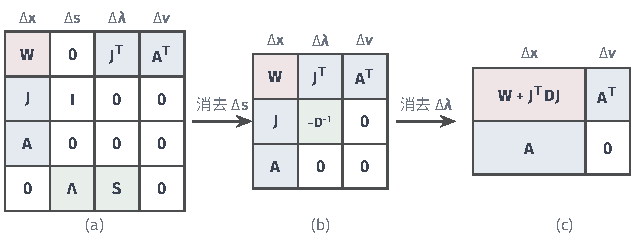
\includegraphics[width=107.5mm]{figures/05-optimization/06-constrained-optimization/tikz/nlipm-kkt-blocks/figure.pdf}
  \caption{Newton方程组的三种等价形式，顶部标出每列对应的方向。红底是含曲率的块，蓝底是约束Jacobian，绿底是对角块，$\bm{D}=\bm{S}^{-1}\bm{\Lambda}$。(a)式~\eqref{eq:nlipm-newton}；(b)消去$\Delta\bm{s}$后的对称鞍点形式；(c)再消去$\Delta\bm{\lambda}$后的压缩形式。}
  \label{fig:nlipm-kkt-blocks}
\end{BookInlineFigure}

把式~\eqref{eq:nlipm-ds}代入式~\eqref{eq:nlipm-dlambda}，再代入第一行，$\Delta\bm{\lambda}$被消去，只剩$\Delta\bm{x}$和$\Delta\bm{\nu}$。记对角矩阵$\bm{D}=\bm{S}^{-1}\bm{\Lambda}$，以及
\begin{equation}
 \tilde{\bm{H}}=\bm{W}+\bm{J}^\top\bm{D}\bm{J},\qquad
 \bm{b}=-\bm{r}_{\mathrm{d}}-\bm{J}^\top\bm{S}^{-1}\bigl(\bm{r}_{\mathrm{c}}+\bm{\Lambda}\bm{r}_{\mathrm{p}}\bigr).
 \label{eq:nlipm-condensed-data}
\end{equation}
方向$\Delta\bm{x}$、$\Delta\bm{\nu}$满足压缩后的鞍点方程
\begin{equation}
 \begin{bmatrix}\tilde{\bm{H}}&\bm{A}^\top\\\bm{A}&\bm{0}\end{bmatrix}
 \begin{bmatrix}\Delta\bm{x}\\\Delta\bm{\nu}\end{bmatrix}
 =\begin{bmatrix}\bm{b}\\-\bm{r}_{\mathrm{e}}\end{bmatrix}.
 \label{eq:nlipm-condensed}
\end{equation}

$\tilde{\bm{H}}$的两部分对应障碍的两种作用：$\bm{J}^\top\bm{D}\bm{J}$在约束法向上加刚度，$\bm{W}$保留目标和约束的弯曲。在式~\eqref{eq:nlipm-newton}的第二种写法里，只消去$\Delta\bm{s}$，保留$\Delta\bm{\lambda}$，得到的矩阵是
\begin{equation}
 \begin{bmatrix}\bm{W}&\bm{J}^\top&\bm{A}^\top\\\bm{J}&-\bm{D}^{-1}&\bm{0}\\\bm{A}&\bm{0}&\bm{0}\end{bmatrix}.
 \label{eq:nlipm-saddle}
\end{equation}
压缩形式维数小，鞍点形式稀疏性好，第~\ref{sec:nlipm-guarantees}节比较它们的代价。

举一个带等式约束的算例，看$\bm{A}$的作用。取下面的矩阵$\tilde{\bm{H}}$和右端$\bm{b}$（稍后的计算过程会在贯穿例的第一轮得到它们），再加一条等式约束$x_1-x_2+1=0$，当前点$(1,2)$满足它，所以$r_{\mathrm{e}}=0$：
\[
 \tilde{\bm{H}}=\begin{bmatrix}7&-2\\-2&9/4\end{bmatrix},\qquad\bm{b}=\begin{bmatrix}8/5\\-19/10\end{bmatrix},\qquad\bm{A}=[1\ \ -1].
\]
由$\bm{A}\Delta\bm{x}=0$，方向只能取$\Delta\bm{x}=\tau(1,1)^\top$。用$(1,1)$左乘第一块方程，$\Delta\nu$相互抵消，得到
\[
 \tfrac{21}{4}\tau=-\tfrac{3}{10},\qquad\text{即}\qquad\tau=-\frac{2}{35}.
\]
再由第一行，$5\tau+\Delta\nu=8/5$，于是$\Delta\nu=66/35$。等式约束的作用是把方向压进切平面，这和第~\ref{chap:quadratic-conic-programming}章的等式约束二次规划一样。

\paragraph{与障碍法的Newton方向比较}
若$\bm{s}=-\bm{g}(\bm{x})$，$\bm{\lambda}=\mu\bm{S}^{-1}\bm{1}$，则$\tilde{\bm{H}}=\nabla^2B_\mu$，两种方法在这一点上的矩阵相同。差别出现在其他点：参数一降，障碍法的乘子估计立刻变成$\mu^+/s_i$，原始—对偶方法的$\lambda_i$则留在当前值，由方程去修正。

回到一维例子，站在$x=-1/2$、$s=3/4$、$\lambda=1$，目标参数$\hat{\mu}=0.05$。这时
\[
 W=2,\quad J=-1,\quad D=\frac43,\quad\tilde{H}=\frac{10}{3},\quad r_{\mathrm{c}}=0.05-0.75=-0.7.
\]
由式~\eqref{eq:nlipm-condensed-data}，$b=-J\,r_{\mathrm{c}}/s=-14/15$，于是
\[
 \Delta x=-0.28,\qquad\Delta s=-0.28,\qquad\Delta\lambda=-0.56.
\]
单位步得到$x=-0.78$、$s=0.47$、$\lambda=0.44$，都留在正确的一侧。同样的起点和目标参数，障碍法的Newton步是$-4.2$。这里的差别和第~\ref{chap:lp-interior-point}章线性化$x_is_i=\mu$而不线性化$s_i=\mu/x_i$是同一个原因。

\paragraph{曲率让残差不再按比例下降}
线性规划中，走步长$\alpha$后等式残差精确地乘以$1-\alpha$。这个性质来自约束是线性的。现在对松弛方程作Taylor展开，走完步长$\alpha$，残差变成
\begin{equation}
 \bm{r}_{\mathrm{p}}^+=(1-\alpha)\bm{r}_{\mathrm{p}}+\bm{\rho}(\alpha),
 \label{eq:nlipm-rp-update}
\end{equation}
其中二阶余项是
\[
 \bm{\rho}(\alpha)=\bm{g}(\bm{x}+\alpha\Delta\bm{x})-\bm{g}(\bm{x})-\alpha\bm{J}\Delta\bm{x}.
\]
若$\nabla g_i$是$L_g$-Lipschitz的，则余项的大小满足
\[
 \lvert\rho_i(\alpha)\rvert\leq\tfrac12L_g\alpha^2\lVert\Delta\bm{x}\rVert_2^2.
\]

贯穿例的$g_1=x_1^2-x_2$是二次的，余项可以精确写出：
\[
 \rho_1(\alpha)=\alpha^2\Delta x_1^2.
\]
图~\ref{fig:nlipm-curved-residual}取一个可行域外的点。线性模型认为约束边界是黄色的切线，走完单位步正好到达；实际约束是抛物线，单位步之后的残差不是零，而是$\Delta x_1^2\approx0.746$。

这个现象还有一个后果：即使当前点满足$\bm{r}_{\mathrm{p}}=\bm{0}$，走一步后也可能变成非零。原始可行性在线性规划中可以一旦达到就永远保持，这里不能。

\begin{BookInlineFigure}
  \centering
  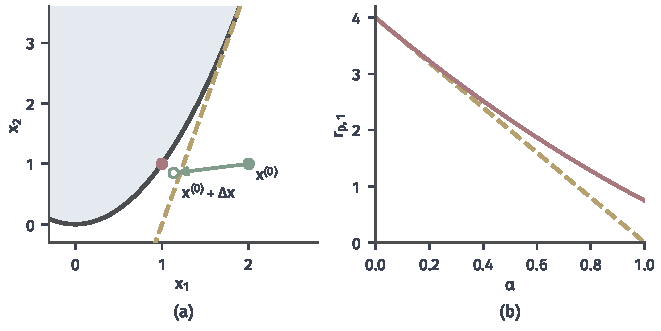
\includegraphics[width=112mm]{figures/05-optimization/06-constrained-optimization/matplotlib/nlipm-curved-residual/figure.pdf}
  \caption{弯的约束使线性化产生误差，贯穿例，起点$\bm{x}^{(0)}=(2,1)$、$\bm{s}=(1,3)$、$\bm{\lambda}=(1,1/3)$、$\sigma=0.2$。(a)深灰粗线是真实边界，黄色虚线是在$\bm{x}^{(0)}$处线性化的边界，绿色箭头是Newton步，红点是$\bm{x}^\star$。(b)红线是实际残差$r_{\mathrm{p},1}$，黄色虚线是线性模型预测的$(1-\alpha)r_{\mathrm{p},1}$，$\alpha=1$时两者相差$\Delta x_1^2$。}
  \label{fig:nlipm-curved-residual}
\end{BookInlineFigure}

\paragraph{线性系统可解，不等于方向好用}
方程组~\eqref{eq:nlipm-condensed}何时有唯一解，答案和约化Hessian有关。

\begin{lemma}[Newton方程的解]
\label{lem:nlipm-newton-solvable}
设$\bm{s},\bm{\lambda}>\bm{0}$，$\bm{A}$满行秩，$\tilde{\bm{H}}$在$\bm{A}$的零空间上正定，即$\bm{A}\bm{d}=\bm{0}$、$\bm{d}\neq\bm{0}$时$\bm{d}^\top\tilde{\bm{H}}\bm{d}>0$。则方程组~\eqref{eq:nlipm-newton}有唯一解。
\end{lemma}

\begin{proof}
消元的每一步都是等价变形，所以只需证明压缩矩阵非奇异。设
\[
 \tilde{\bm{H}}\bm{d}+\bm{A}^\top\bm{w}=\bm{0},\qquad\bm{A}\bm{d}=\bm{0}.
\]
用$\bm{d}^\top$左乘第一式，并用第二式，得到
\[
 \bm{d}^\top\tilde{\bm{H}}\bm{d}=0.
\]
由正定性$\bm{d}=\bm{0}$。于是$\bm{A}^\top\bm{w}=\bm{0}$，由满行秩$\bm{w}=\bm{0}$。
\end{proof}

这个条件比“系数矩阵非奇异”强。矩阵非奇异时方程也有唯一解，但方向可能完全不对。下面的引理说明正定性的真正用途：它保证方向使障碍目标下降。这里的障碍目标把松弛也当作变量，写成
\[
 \psi_{\hat{\mu}}(\bm{x},\bm{s})=f(\bm{x})-\hat{\mu}\sum_{i=1}^m\log s_i.
\]

\begin{lemma}[方向与障碍目标]
\label{lem:nlipm-descent}
设$\bm{r}_{\mathrm{p}}=\bm{0}$，$\bm{r}_{\mathrm{e}}=\bm{0}$，方向由式~\eqref{eq:nlipm-newton}给出，其中目标参数取$\hat{\mu}$。则$\psi_{\hat{\mu}}$沿方向的一阶变化满足
\begin{equation}
 \nabla f^\top\Delta\bm{x}-\hat{\mu}\,\bm{1}^\top\bm{S}^{-1}\Delta\bm{s}=-\Delta\bm{x}^\top\tilde{\bm{H}}\Delta\bm{x}.
 \label{eq:nlipm-descent}
\end{equation}
\end{lemma}

\begin{proof}
由$\bm{r}_{\mathrm{d}}$的定义和$\bm{A}\Delta\bm{x}=\bm{0}$、$\bm{J}\Delta\bm{x}=-\Delta\bm{s}$，有
\[
 \nabla f^\top\Delta\bm{x}=\bm{r}_{\mathrm{d}}^\top\Delta\bm{x}+\bm{\lambda}^\top\Delta\bm{s}.
\]
互补残差满足
\[
 \bm{S}^{-1}\bm{r}_{\mathrm{c}}=\hat{\mu}\bm{S}^{-1}\bm{1}-\bm{\lambda}.
\]
用$\Delta\bm{x}^\top$左乘式~\eqref{eq:nlipm-condensed}的第一块，并代入上式，得到
\[
 \Delta\bm{x}^\top\tilde{\bm{H}}\Delta\bm{x}=-\bm{r}_{\mathrm{d}}^\top\Delta\bm{x}+(\hat{\mu}\bm{S}^{-1}\bm{1}-\bm{\lambda})^\top\Delta\bm{s}.
\]
由第二式解出$\bm{r}_{\mathrm{d}}^\top\Delta\bm{x}$，代入第一式，$\bm{\lambda}^\top\Delta\bm{s}$相互抵消，即得结论。
\end{proof}

所以$\tilde{\bm{H}}$在切空间上不正定时，$\Delta\bm{x}$可能是上升方向。图~\ref{fig:nlipm-regularization}取圆盘外部的例子，$\mu=0.1$，在$\bm{x}=(0.35,1.08)^\top$处的特征值是
\[
 -0.320,\qquad 7.352.
\]
Newton方向的一阶变化是$\nabla B_\mu^\top\bm{d}=+0.947$，它是上升方向，指向鞍点。系数矩阵非奇异，线性方程解得毫无困难，得到的却是错误的方向。

补救办法是\term{矩阵正则化}（matrix regularization）：把$\tilde{\bm{H}}$换成$\tilde{\bm{H}}+\delta_{\mathrm{w}}\bm{I}$，$\delta_{\mathrm{w}}\geq0$逐步增大，直到切空间上正定。例中取$\delta_{\mathrm{w}}=0.47$，新方向的一阶变化是$-2.73$，变成下降方向。

怎样判断切空间上正定？实际中不直接算切空间，而看鞍点矩阵的惯性，即正、负、零特征值的个数。$\bm{A}$满行秩时，$\tilde{\bm{H}}$在零空间上正定，当且仅当矩阵~\eqref{eq:nlipm-condensed}的惯性是$(n,p,0)$。分解$\bm{L}\bm{D}\bm{L}^\top$时可以直接读出惯性，所以试探$\delta_{\mathrm{w}}$只要重复分解。这个判据的证明要用到Sylvester惯性定律，读者可查阅专著\scite{math-nocedal2006numerical}。

\begin{BookInlineFigure}
  \centering
  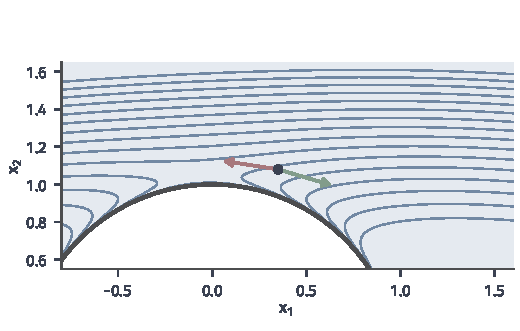
\includegraphics[width=88mm]{figures/05-optimization/06-constrained-optimization/matplotlib/nlipm-regularization/figure.pdf}
  \caption{曲率不定时的方向，圆盘外部的例子，$\mu=0.1$。深灰粗线是约束边界，蓝线是$B_\mu$的等值线，黑点是当前点。红色箭头是未修正的Newton方向，指向上升一侧的鞍点（为便于观察，按比例缩短）；绿色箭头是加上$\delta_{\mathrm{w}}\bm{I}$之后的方向，沿下降方向走向右侧的极小点。}
  \label{fig:nlipm-regularization}
\end{BookInlineFigure}

另一类困难来自约束退化。若活动约束或等式约束的梯度线性相关，$\bm{A}$不再满行秩，矩阵奇异或接近奇异。常用的办法是在右下角加上$-\delta_{\mathrm{c}}\bm{I}$，相当于允许等式约束有微小的违反。数值尺度也要处理：把某条约束乘以$1000$，$\bm{D}$和残差的数值都跟着变，通常先对目标和约束的梯度作缩放。这些修改的代价是方向不再是真正的Newton方向，第~\ref{sec:nlipm-stopping}小节会说明为什么最后要按未经修改的问题检查结果。

\subsection{步长与中心性}
\label{sec:nlipm-step}

得到方向后，还要回答走多远。这里有三件事彼此独立：不能越过边界，这一步要确实有进展，迭代点不能离路径太远。

\paragraph{到边界的比例规则}
第一件事沿用第~\ref{chap:lp-interior-point}章的做法，只是作用在$(\bm{s},\bm{\lambda})$上：
\begin{equation}
 \alpha_{\max}=\min\Bigl\{\min_{\Delta s_i<0}\frac{s_i}{-\Delta s_i},\ \min_{\Delta\lambda_i<0}\frac{\lambda_i}{-\Delta\lambda_i}\Bigr\},\qquad
 \alpha=\min\{1,\ \eta\,\alpha_{\max}\},
 \label{eq:nlipm-alpha}
\end{equation}
其中$\eta\in(0,1)$，没有负分量时约定$\alpha_{\max}=+\infty$。

这条规则保护的是$\bm{s}>\bm{0}$，而不是$\bm{g}(\bm{x})<\bm{0}$。当$\bm{r}_{\mathrm{p}}\neq\bm{0}$时，$\bm{x}$可以暂时越过约束边界。这是原始—对偶方法相对于障碍法的自由，也是第~\ref{sec:nlipm-stopping}小节必须检查原约束的原因。

实现中常对原始变量和对偶变量用不同的步长，因为线性规划中“单一步长让互补量精确下降”的理由在这里已经不成立。下面的算例为了便于手算，仍用单一步长。

\paragraph{残差检验}
满足比例规则的步长仍可能太长，因为式~\eqref{eq:nlipm-rp-update}的余项和$\bm{W}$的变化都没有进入线性模型。最直接的检验是看方程残差有没有变小。把方程组写成$\bm{F}_{\hat{\mu}}(\bm{z})=\bm{0}$，其中$\bm{z}=(\bm{x},\bm{s},\bm{\lambda},\bm{\nu})$，要求
\begin{equation}
 \lVert\bm{F}_{\hat{\mu}}(\bm{z}+\alpha\Delta\bm{z})\rVert_2\leq(1-c\,\alpha)\lVert\bm{F}_{\hat{\mu}}(\bm{z})\rVert_2,
 \label{eq:nlipm-residual-armijo}
\end{equation}
其中$c\in(0,1)$是小常数，不满足时把$\alpha$减半。

\begin{lemma}[Newton方向使残差下降]
\label{lem:nlipm-residual-descent}
设$\bm{F}_{\hat{\mu}}$连续可微，其Jacobian矩阵在$\bm{z}$处非奇异，$\Delta\bm{z}$是Newton方向，$\bm{F}_{\hat{\mu}}(\bm{z})\neq\bm{0}$。则$\alpha>0$足够小时，式~\eqref{eq:nlipm-residual-armijo}成立。
\end{lemma}

\begin{proof}
记
\[
 \Theta(\alpha)=\tfrac12\lVert\bm{F}_{\hat{\mu}}(\bm{z}+\alpha\Delta\bm{z})\rVert_2^2.
\]
由Newton方程$\bm{G}\Delta\bm{z}=-\bm{F}$，其中$\bm{G}$是Jacobian矩阵，有
\[
 \Theta'(0)=\bm{F}^\top\bm{G}\Delta\bm{z}=-\lVert\bm{F}\rVert_2^2.
\]
于是残差范数的展开是
\[
 \sqrt{2\Theta(\alpha)}=\lVert\bm{F}\rVert_2(1-\alpha)+o(\alpha).
\]
而$c<1$，所以$\alpha$足够小时不等式成立。
\end{proof}

这个检验简单，但有明显的盲区：它只看方程残差，分不清极小点和鞍点。方程组的任何解都能把它压到零，包括前面的$x=2$（若不靠正性挡住）和各种局部极大点。所以在非凸问题上，更常用的检验还要看目标。

\paragraph{过滤器}
一个直接想法是把约束违反量和障碍目标合成一个数，用它来比较。这需要一个权重，取大了算法只管可行，取小了只管目标。\term{过滤器}（filter）绕开这个权重，它把每一步看成二维平面上的一个点：
\begin{equation}
 \theta(\bm{z})=\bigl\lVert(\bm{h}(\bm{x}),\ \bm{g}(\bm{x})+\bm{s})\bigr\rVert_2,\qquad
 \psi_\mu(\bm{x},\bm{s})=f(\bm{x})-\mu\sum_{i=1}^m\log s_i.
 \label{eq:nlipm-filter-pair}
\end{equation}

算法保存一些历史点$(\theta_l,\psi_l)$，试探点只要不被其中任何一个点支配，就可以接受，也就是对每个$l$，要么$\theta$比$\theta_l$小，要么$\psi_\mu$比$\psi_l$小。图~\ref{fig:nlipm-filter}中有三个历史点$(0.2,4)$、$(0.5,3)$、$(1,2.5)$。

试探点A$=(0.3,3.2)$的$\theta$比$(0.5,3)$和$(1,2.5)$都小，$\psi_\mu$又比$(0.2,4)$小，所以被接受。试探点B$=(0.6,3.5)$的两个分量都比$(0.5,3)$差，被拒绝。两项指标各有高低的点互不否定，两项都差的点才被淘汰。

实际的过滤器要求有一定幅度的改进，例如$\theta\leq(1-\gamma_\theta)\theta_l$或$\psi_\mu\leq\psi_l-\gamma_\psi\theta_l$，否则可能无穷地接受改进极小的点。如果步长被缩到极小仍不能接受，算法转入\term{可行性恢复}（feasibility restoration）阶段，暂时放下目标，只减小$\theta$。

\begin{BookInlineFigure}
  \centering
  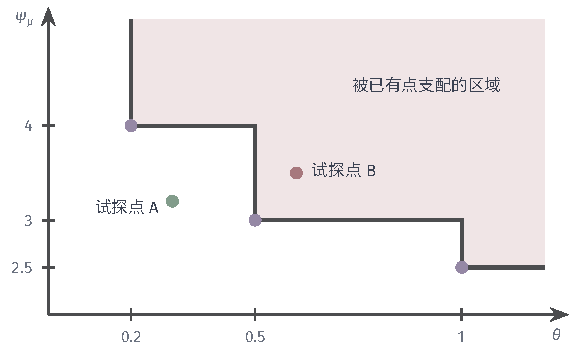
\includegraphics[width=97mm]{figures/05-optimization/06-constrained-optimization/tikz/nlipm-filter/figure.pdf}
  \caption{过滤器。横轴是约束违反量$\theta$，纵轴是障碍目标$\psi_\mu$。紫点是已保存的历史点，红底是被它们支配的区域。绿点A不被任何历史点支配，可以接受；红点B落在被支配区域内，被拒绝。}
  \label{fig:nlipm-filter}
\end{BookInlineFigure}

\paragraph{保持正性与靠近中心是两回事}
到边界的比例规则只保证$s_i,\lambda_i>0$。点可以严格在内部，却让某个乘积比平均值小几千倍，这时下一轮的Newton步很可能被这个小乘积卡住。沿用第~\ref{chap:lp-interior-point}章的度量，定义中心性
\begin{equation}
 \xi=\frac{\min_is_i\lambda_i}{\mu}\in(0,1].
 \label{eq:nlipm-centrality}
\end{equation}
要求$\xi\geq\gamma$（例如$\gamma=10^{-3}$）的集合称为\term{宽邻域}（wide neighborhood）。

图~\ref{fig:nlipm-wspace}把贯穿例的迭代画在$(s_1\lambda_1,s_2\lambda_2)$平面上。中心路径在这个平面上是对角线。绿线取$\sigma=0.2$，$\eta=0.9$，轨迹贴着对角线，中心性最低为$0.49$。

黄线取$\sigma=0.02$，$\eta=0.9999$，每步都几乎走到边界，第一步就让中心性掉到$10^{-3}$，再走两轮才恢复到$0.9$以上。正性两条线都保持了，靠近中心的程度却差别很大。

\begin{BookInlineFigure}
  \centering
  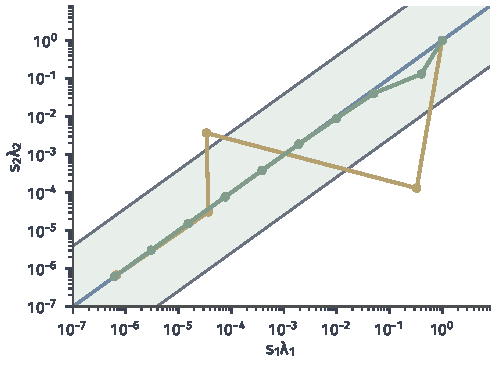
\includegraphics[width=84mm]{figures/05-optimization/06-constrained-optimization/matplotlib/nlipm-wspace/figure.pdf}
  \caption{互补乘积平面，对数坐标，贯穿例。蓝线是$s_1\lambda_1=s_2\lambda_2$，即中心路径；浅绿带是宽邻域$\xi\geq0.05$，灰线是其边界。绿线是$\sigma=0.2$、$\eta=0.9$的迭代，黄线是$\sigma=0.02$、$\eta=0.9999$的迭代，后者离开了浅绿带。}
  \label{fig:nlipm-wspace}
\end{BookInlineFigure}

\paragraph{计算过程}
下面把一轮迭代写成具体步骤，并在例~\eqref{eq:nlipm-running}上逐轮计算。取固定的中心化参数$\sigma=0.2$、比例$\eta=0.9$、残差检验常数$c=10^{-4}$，容差$\varepsilon=10^{-6}$。例中没有等式约束，含$\bm{A}$、$\bm{\nu}$的量都不出现。

\needspace{6\baselineskip}
\paragraph{变量}
\begin{itemize}
 \item $\bm{x}\in\mathbb{R}^n$：原始变量。$\bm{s}\in\mathbb{R}^m$：松弛，全部分量为正。
 \item $\bm{\lambda}\in\mathbb{R}^m$：不等式乘子，全部分量为正。$\bm{\nu}\in\mathbb{R}^p$：等式乘子。
 \item $\mu$、$\hat{\mu}$：平均互补量和本轮的目标参数，由式~\eqref{eq:nlipm-mu}给出。
 \item $\bm{r}_{\mathrm{d}},\bm{r}_{\mathrm{e}},\bm{r}_{\mathrm{p}},\bm{r}_{\mathrm{c}}$：式~\eqref{eq:nlipm-residuals}的四个残差，维数依次是$n$、$p$、$m$、$m$。
 \item $\bm{W}$、$\bm{D}$、$\tilde{\bm{H}}$、$\bm{b}$：Lagrange Hessian、对角缩放、压缩矩阵和右端，分别由式~\eqref{eq:nlipm-lagrange-hessian}、\eqref{eq:nlipm-condensed-data}给出。
 \item $\Delta\bm{x},\Delta\bm{s},\Delta\bm{\lambda},\Delta\bm{\nu}$：本轮的方向；$\alpha_{\max},\alpha$：最大步长和实际步长。
\end{itemize}

\paragraph{初始化}
取$\bm{x}^{(0)}$、$\bm{s}^{(0)}>\bm{0}$、$\bm{\lambda}^{(0)}>\bm{0}$和$\bm{\nu}^{(0)}$，令$t=0$；起点的选取由下一节讨论。例中取严格可行的点，并让两个乘积相等：
\[
 \bm{x}^{(0)}=\begin{bmatrix}1\\2\end{bmatrix},\qquad
 \bm{s}^{(0)}=-\bm{g}(\bm{x}^{(0)})=\begin{bmatrix}1\\2\end{bmatrix},\qquad
 \bm{\lambda}^{(0)}=\begin{bmatrix}1\\1/2\end{bmatrix}.
\]

\needspace{6\baselineskip}
\paragraph{每轮更新}
在第$t$轮，以$(\bm{x}^{(t)},\bm{s}^{(t)},\bm{\lambda}^{(t)},\bm{\nu}^{(t)})$为当前点：
\begin{enumerate}
 \item \textbf{计算残差并检查停止。}按式~\eqref{eq:nlipm-mu}、\eqref{eq:nlipm-residuals}计算$\mu$和残差。若$\lVert\bm{r}_{\mathrm{d}}\rVert_\infty$、$\lVert\bm{r}_{\mathrm{e}}\rVert_\infty$、$\lVert\bm{r}_{\mathrm{p}}\rVert_\infty$和$\max_is_i\lambda_i$都不超过$\varepsilon$，停止并输出当前点。

 例中第一轮$\mu^{(0)}=1$，$\hat{\mu}=0.2$，
 \[
  \bm{r}_{\mathrm{d}}=\begin{bmatrix}-2\\2\end{bmatrix}+\begin{bmatrix}2\\-1/2\end{bmatrix}=\begin{bmatrix}0\\3/2\end{bmatrix},\quad
  \bm{r}_{\mathrm{p}}=\bm{0},\quad
  \bm{r}_{\mathrm{c}}=\begin{bmatrix}-4/5\\-4/5\end{bmatrix}.
 \]

 \item \textbf{形成压缩方程。}由式~\eqref{eq:nlipm-lagrange-hessian}计算$\bm{W}$，由式~\eqref{eq:nlipm-condensed-data}计算$\tilde{\bm{H}}$和$\bm{b}$。检查惯性，必要时加$\delta_{\mathrm{w}}\bm{I}$。

 例中第一轮$\lambda_1=1$，所以$\bm{W}=\operatorname{diag}(3,1)$，而$\bm{D}=\operatorname{diag}(1,1/4)$，$\bm{J}$的两行是$(2,-1)$和$(0,1)$，所以
 \[
  \tilde{\bm{H}}=\begin{bmatrix}3&0\\0&1\end{bmatrix}+\begin{bmatrix}4&-2\\-2&5/4\end{bmatrix}=\begin{bmatrix}7&-2\\-2&9/4\end{bmatrix}.
 \]
 又$\bm{S}^{-1}\bm{r}_{\mathrm{c}}=(-4/5,-2/5)^\top$，于是
 \[
  \bm{b}=-\begin{bmatrix}0\\3/2\end{bmatrix}-\begin{bmatrix}-8/5\\2/5\end{bmatrix}=\begin{bmatrix}8/5\\-19/10\end{bmatrix}.
 \]
 这个矩阵的两个顺序主子式$7$和$47/4$都是正的，因此正定，不需要修正。

 \item \textbf{求方向。}解式~\eqref{eq:nlipm-condensed}得到$\Delta\bm{x}$、$\Delta\bm{\nu}$，再由式~\eqref{eq:nlipm-ds}、\eqref{eq:nlipm-dlambda}回代。

 例中第一轮
 \[
  \Delta\bm{x}=\Bigl(-\frac{4}{235},\,-\frac{202}{235}\Bigr)^\top\approx(-0.0170,\,-0.8596)^\top.
 \]
 回代得到
 \[
  \Delta\bm{s}\approx(-0.8255,\,0.8596)^\top,\qquad\Delta\bm{\lambda}\approx(0.0255,\,-0.6149)^\top.
 \]

 \item \textbf{确定步长。}由式~\eqref{eq:nlipm-alpha}得到候选$\alpha$，再用式~\eqref{eq:nlipm-residual-armijo}（或过滤器）检验，不通过则把$\alpha$减半。

 例中第一轮只有$s_1$和$\lambda_2$在减小，比值分别是$1.2113$和$0.8131$，所以
 \[
  \alpha_{\max}\approx0.8131,\qquad\alpha=0.9\,\alpha_{\max}\approx0.7318.
 \]
 残差范数从$1.8788$降到$0.4559$，检验通过，不需要回溯。

 \item \textbf{更新。}令
 \begin{equation}
  \begin{aligned}
  \bm{x}^{(t+1)}&=\bm{x}^{(t)}+\alpha\Delta\bm{x},\quad&
  \bm{s}^{(t+1)}&=\bm{s}^{(t)}+\alpha\Delta\bm{s},\\
  \bm{\lambda}^{(t+1)}&=\bm{\lambda}^{(t)}+\alpha\Delta\bm{\lambda},\quad&
  \bm{\nu}^{(t+1)}&=\bm{\nu}^{(t)}+\alpha\Delta\bm{\nu},
  \end{aligned}
  \label{eq:nlipm-update}
 \end{equation}
 然后令$t\leftarrow t+1$，回到第1步。

 例中第一轮
 \[
  \begin{gathered}
  \bm{x}^{(1)}\approx(0.9875,\,1.3709)^\top,\\
  \bm{s}^{(1)}\approx(0.3958,\,2.6291)^\top,\qquad\bm{\lambda}^{(1)}\approx(1.0187,\,0.0500)^\top.
  \end{gathered}
 \]
 这时$\bm{r}_{\mathrm{p}}$不再为零，第一个分量是$\alpha^2\Delta x_1^2\approx1.55\times10^{-4}$，这正是式~\eqref{eq:nlipm-rp-update}的余项。
\end{enumerate}

例中第二轮的中间量如下。当前$\mu^{(1)}=0.2673$，$\hat{\mu}=0.0535$，两个乘积是$0.4032$和$0.1314$，于是
\[
 \bm{r}_{\mathrm{d}}\approx(-0.0005,\,0.4022)^\top,\qquad\bm{r}_{\mathrm{c}}\approx(-0.3498,\,-0.0780)^\top.
\]
压缩矩阵和右端是
\[
 \tilde{\bm{H}}\approx\begin{bmatrix}13.076&-5.083\\-5.083&3.592\end{bmatrix},\qquad\bm{b}\approx\begin{bmatrix}1.745\\-1.256\end{bmatrix}.
\]
解方程组并回代，得到
\[
 \begin{gathered}
 \Delta\bm{x}\approx(-0.0054,\,-0.3572)^\top,\\
 \Delta\bm{s}\approx(-0.3467,\,0.3572)^\top,\qquad\Delta\bm{\lambda}\approx(0.0086,\,-0.0365)^\top.
 \end{gathered}
\]
这一轮$\alpha_{\max}\approx1.1418$，$0.9\alpha_{\max}>1$，所以取$\alpha=1$。新的点是
\[
 \begin{gathered}
 \bm{x}^{(2)}\approx(0.9821,\,1.0137)^\top,\\
 \bm{s}^{(2)}\approx(0.0492,\,2.9863)^\top,\qquad\bm{\lambda}^{(2)}\approx(1.0273,\,0.0135)^\top.
 \end{gathered}
\]

此后每轮都取$\alpha=1$，平均互补量几乎每轮乘以$0.2$。表~\ref{tab:nlipm-run}列出全部迭代。第$9$轮后所有残差和乘积都不超过$10^{-6}$，算法停止。

\begin{BookInlineTable}
  \centering
  \footnotesize
  \begin{tabular}{@{}ccccccccc@{}}
    \toprule
    $t$ & $x_1^{(t)}$ & $x_2^{(t)}$ & $s_1^{(t)}$ & $\lambda_1^{(t)}$ & $\mu^{(t)}$ & $\lVert\bm{r}_{\mathrm{d}}\rVert_\infty$ & $\lVert\bm{r}_{\mathrm{p}}\rVert_\infty$ & $\alpha$\\
    \midrule
    0 & 1.0000 & 2.0000 & 1.0000 & 1.0000 & 1.00 & 1.5 & 0 & 0.732\\
    1 & 0.9875 & 1.3709 & 0.3958 & 1.0187 & 0.267 & 0.40 & $1.6\mathrm{e}{-4}$ & 1\\
    2 & 0.9821 & 1.0137 & 0.0492 & 1.0272 & 0.0455 & $9.3\mathrm{e}{-5}$ & $2.9\mathrm{e}{-5}$ & 1\\
    3 & 0.9963 & 1.0023 & 0.0099 & 1.0053 & $9.5\mathrm{e}{-3}$ & $6.2\mathrm{e}{-4}$ & $2.0\mathrm{e}{-4}$ & 1\\
    4 & 0.9993 & 1.0005 & 0.0019 & 1.0011 & $1.9\mathrm{e}{-3}$ & $2.5\mathrm{e}{-5}$ & $8.9\mathrm{e}{-6}$ & 1\\
    5 & 0.9999 & 1.0001 & 0.0004 & 1.0002 & $3.8\mathrm{e}{-4}$ & $1.0\mathrm{e}{-6}$ & $3.4\mathrm{e}{-7}$ & 1\\
    6 & 1.0000 & 1.0000 & 0.0001 & 1.0000 & $7.6\mathrm{e}{-5}$ & $4.1\mathrm{e}{-8}$ & $1.4\mathrm{e}{-8}$ & 1\\
    7 & 1.0000 & 1.0000 & 0.0000 & 1.0000 & $1.5\mathrm{e}{-5}$ & $1.6\mathrm{e}{-9}$ & $5.4\mathrm{e}{-10}$ & 1\\
    8 & 1.0000 & 1.0000 & 0.0000 & 1.0000 & $3.1\mathrm{e}{-6}$ & $6.5\mathrm{e}{-11}$ & $2.2\mathrm{e}{-11}$ & 1\\
    9 & 1.0000 & 1.0000 & 0.0000 & 1.0000 & $6.1\mathrm{e}{-7}$ & $2.6\mathrm{e}{-12}$ & $8.7\mathrm{e}{-13}$ & \\
    \bottomrule
  \end{tabular}
  \caption{贯穿例的逐轮中间量，$\sigma=0.2$、$\eta=0.9$。第$t$行的$\alpha$是从第$t$个点出发那一轮的步长。全部$\alpha$都未经回溯。}
  \label{tab:nlipm-run}
\end{BookInlineTable}

最终得到
\[
 \hat{\bm{x}}\approx(1.0000,\,1.0000)^\top,\qquad\hat{\bm{\lambda}}\approx(1.0000,\,2\times10^{-7})^\top,
\]
目标误差约$6.1\times10^{-7}$。第$3$轮的驻定残差比第$2$轮大，这说明残差并不单调下降，因为每轮的目标$\hat{\mu}$都在变。

图~\ref{fig:nlipm-iterates}比较这条轨迹与障碍法（$\tau=0.2$）。两者起点相同，绿线直接朝解走，$9$轮停止；黄线先走到$\mu=1$的碗底，再沿路径前进，在同样的精度下用了$34$个Newton步。图~\ref{fig:nlipm-residual-curves}给出各残差随轮次的变化，可以看到$\lVert\bm{r}_{\mathrm{p}}\rVert_\infty$从零升起，这是约束弯曲带来的。

\begin{BookInlineFigure}
  \centering
  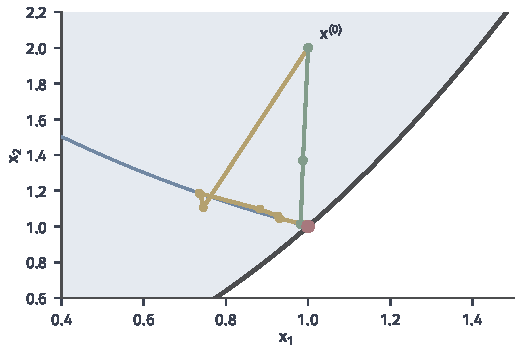
\includegraphics[width=88mm]{figures/05-optimization/06-constrained-optimization/matplotlib/nlipm-iterates/figure.pdf}
  \caption{贯穿例的迭代点，局部放大。蓝线是中心路径，绿线是$\sigma=0.2$的原始—对偶迭代，黄线是$\tau=0.2$的障碍法的Newton迭代点，红点是$\bm{x}^\star$，深灰粗线是约束边界。两者都从$(1,2)$出发。}
  \label{fig:nlipm-iterates}
\end{BookInlineFigure}

\begin{BookInlineFigure}
  \centering
  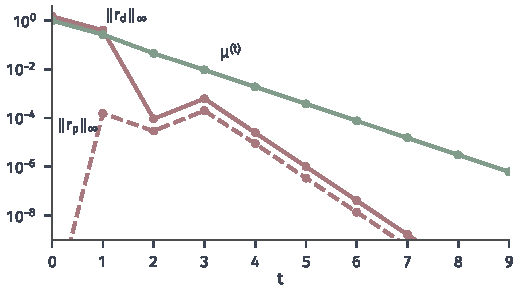
\includegraphics[width=88mm]{figures/05-optimization/06-constrained-optimization/matplotlib/nlipm-residual-curves/figure.pdf}
  \caption{贯穿例的残差历史，对数纵轴。红色实线是$\lVert\bm{r}_{\mathrm{d}}\rVert_\infty$，红色虚线是$\lVert\bm{r}_{\mathrm{p}}\rVert_\infty$（第$0$轮为零，图中从下方进入），绿线是$\mu^{(t)}$。}
  \label{fig:nlipm-residual-curves}
\end{BookInlineFigure}

\paragraph{预测—校正要重新核对条件}
第~\ref{chap:lp-interior-point}章的预测—校正可以直接搬用：先解$\sigma=0$的方程组，用试走后的互补量选$\sigma$，再把$\Delta s_i^{\mathrm{a}}\Delta\lambda_i^{\mathrm{a}}$移到右端。两次求解共用一次分解。例中第一轮，预测步的结果是
\[
 \alpha^{\mathrm{a}}\approx0.7015,\qquad\mu^{\mathrm{a}}\approx0.1640,\qquad\sigma\approx0.0044.
\]
校正后取到$\alpha\approx0.8556$，平均互补量降到$0.2085$，而固定$\sigma=0.2$时是$0.2673$。代价也很明显：两个乘积变成$0.0997$和$0.3174$，不再相等。

搬用时有三点要重新核对。校正项只补偿了互补方程的二阶项，约束的二阶余项$\bm{\rho}$并没有补偿。预测步用的$\bm{W}$若经过了正则化，二阶项的估计就是另一个问题的量。线性规划中单位步之后等式残差恰好消失，这里没有这个性质，所以校正之后的步长仍要过残差或过滤器的检验，单靠比例规则不够。

\section{初始化与精度}
\label{sec:nlipm-init-accuracy}

前两节都假设手里已经有一个能用的起点，也没有说算到什么程度可以停。本节要回答这两个问题：障碍路径和原始—对偶迭代分别需要怎样的起点，以及停下来的点能对原问题说什么。

\subsection{初始点的构造}
\label{sec:nlipm-initial-point}

两类方法对起点的要求不同。障碍法要计算$\log(-g_i(\bm{x}))$，所以每个迭代点都必须严格可行。原始—对偶方法的方程里不出现$\log(-g_i)$，它只要求$\bm{s},\bm{\lambda}>\bm{0}$，$\bm{x}$可以在可行域之外。

\paragraph{辅助可行性问题}
需要严格可行点时，可以先解一个以“最大违反量”为目标的问题：
\begin{equation}
 \min_{\bm{x},\rho}\ \rho\quad\text{s.t.}\quad g_i(\bm{x})\leq\rho\ (i=1,\ldots,m),\quad\bm{h}(\bm{x})=\bm{0}.
 \label{eq:nlipm-phase-one}
\end{equation}
这个问题的严格可行点是现成的：只要有一个满足等式的$\bm{x}$，取$\rho>\max_ig_i(\bm{x})$即可。线性等式可以解线性方程组得到这样的$\bm{x}$，非线性等式本身就是一个方程求根的问题，这里并没有绕过它。

设$\rho^\star$是最优值。在凸问题上，它的符号给出三种结论：

\begin{itemize}
 \item $\rho^\star<0$：最优点严格可行，可以作为障碍法的起点。
 \item $\rho^\star=0$：原问题可行或处在可行的边缘，但没有严格可行点。
 \item $\rho^\star>0$：原问题不可行。
\end{itemize}

在非凸问题上，算法只能找到局部解，$\rho>0$的局部解不能说明原问题不可行。

贯穿例从$\bm{x}^{(0)}=(2,1)^\top$开始，$\bm{g}=(3,-3)^\top$，取$\rho=4$就严格可行。解$\min\max\{x_1^2-x_2,\ x_2-4\}$时，$x_1=0$使第一项最小，再让$-x_2=x_2-4$，得到
\[
 \bm{x}=(0,2)^\top,\qquad\rho^\star=-2.
\]
这正是解析中心。图~\ref{fig:nlipm-phase-one}显示，随着$\rho$减小，放宽后的区域逐层收缩到这一点。实际上不必解到最优，一旦$\rho<0$就可以提前停下，这时得到的点已经是严格可行的。

\begin{BookInlineFigure}
  \centering
  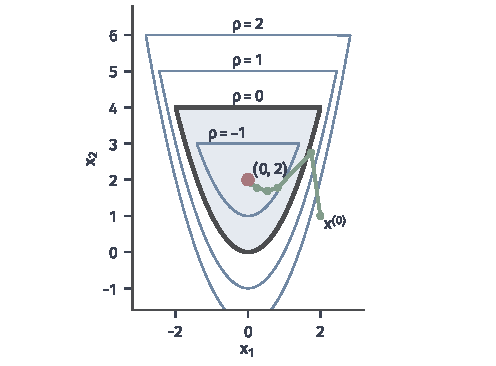
\includegraphics[width=84mm]{figures/05-optimization/06-constrained-optimization/matplotlib/nlipm-phase-one/figure.pdf}
  \caption{贯穿例的辅助问题~\eqref{eq:nlipm-phase-one}。蓝线是$\max_ig_i(\bm{x})=\rho$的水平集，深灰粗线是$\rho=0$，即原可行集的边界。绿线是从可行域外的$\bm{x}^{(0)}=(2,1)$出发、用障碍法解这个问题的迭代点，红点是解$(0,2)$，这里$\rho^\star=-2$。}
  \label{fig:nlipm-phase-one}
\end{BookInlineFigure}

\paragraph{从非零的原始残差开始}
原始—对偶方法不用先解辅助问题。任取$\bm{x}^{(0)}$，再选一个正的下限$\delta$，令
\begin{equation}
 s_i^{(0)}=\max\bigl\{-g_i(\bm{x}^{(0)}),\ \delta\bigr\},\qquad\lambda_i^{(0)}=\frac{\mu^{(0)}}{s_i^{(0)}}.
 \label{eq:nlipm-infeasible-start}
\end{equation}
这样所有乘积都等于$\mu^{(0)}$，起点在互补方程的意义下是居中的。约束已满足的分量，$\bm{r}_{\mathrm{p}}$是零，被违反的分量，$\bm{r}_{\mathrm{p}}$非零。

要记住的是，$\bm{s},\bm{\lambda}>\bm{0}$并不意味着$\bm{g}(\bm{x})+\bm{s}=\bm{0}$已经成立。正性是起点就满足的，松弛方程是迭代要逐步解的。在$\bm{r}_{\mathrm{p}}\neq\bm{0}$的点上，$s_i>0$也不告诉我们$g_i(\bm{x})<0$。

贯穿例取$\bm{x}^{(0)}=(2,1)^\top$，$\delta=1$，$\mu^{(0)}=1$，由式~\eqref{eq:nlipm-infeasible-start}得到
\[
 \bm{s}^{(0)}=\begin{bmatrix}1\\3\end{bmatrix},\qquad\bm{\lambda}^{(0)}=\begin{bmatrix}1\\1/3\end{bmatrix},\qquad\bm{r}_{\mathrm{p}}=\begin{bmatrix}4\\0\end{bmatrix}.
\]
仍取$\sigma=0.2$，按式~\eqref{eq:nlipm-condensed-data}算出
\[
 \tilde{\bm{H}}=\begin{bmatrix}19&-4\\-4&19/9\end{bmatrix},\qquad\bm{b}\approx\begin{bmatrix}-15.8\\3.133\end{bmatrix}.
\]
解出方向并回代，得到
\[
 \Delta\bm{x}\approx(-0.8636,\,-0.1521)^\top,\qquad\Delta\bm{s}\approx(-0.6977,\,0.1521)^\top.
\]

这一轮取到$\alpha=1$。线性规划中单位步会让等式残差归零，这里第一个分量却变成$\Delta x_1^2\approx0.7458$，这就是图~\ref{fig:nlipm-curved-residual}(b)的右端点。

第二轮$\alpha\approx0.946$，$r_{\mathrm{p},1}$降到$0.059$，再一轮之后降到$1.7\times10^{-5}$。图~\ref{fig:nlipm-infeasible-start}显示，残差下降虽然不再是精确的比例，但在这个例子上很快就跟上了互补量。

\begin{BookInlineFigure}
  \centering
  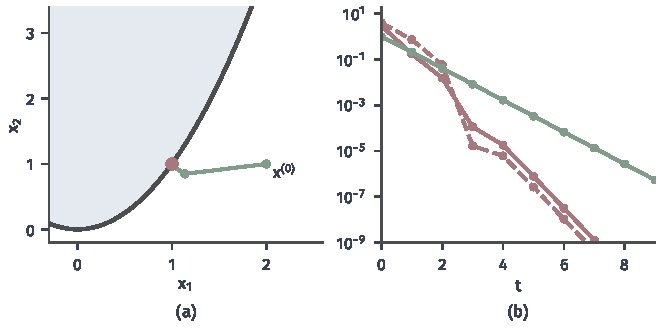
\includegraphics[width=112mm]{figures/05-optimization/06-constrained-optimization/matplotlib/nlipm-infeasible-start/figure.pdf}
  \caption{从可行域外启动，贯穿例，$\sigma=0.2$、$\eta=0.9$。(a)绿线是迭代点，从$(2,1)$进入可行域附近，红点是$\bm{x}^\star$。(b)红色虚线是$\lVert\bm{r}_{\mathrm{p}}\rVert_\infty$，红色实线是$\lVert\bm{r}_{\mathrm{d}}\rVert_\infty$，绿线是$\mu^{(t)}$。}
  \label{fig:nlipm-infeasible-start}
\end{BookInlineFigure}

\paragraph{不收敛到可行点的情形}
线性化的约束可能和当前的残差彼此矛盾。看不可行的一维约束$g(x)=x^2+1\leq0$。残差$x^2+1+s$在$s>0$上没有零点，迭代会被吸引到$x=0$、$s\to0$，这一点上$J=2x=0$，线性化的约束不再能改变残差。这是约束违反量的一个驻点，不是原问题的解。

对凸问题，这样的点可以变成证书。若存在$\bm{w}\geq\bm{0}$，使$\inf_{\bm{x}}\sum_iw_ig_i(\bm{x})>0$，则约束一定无解，因为可行点会让这个和不大于零。上面的例子取$w=1$，$\inf_x(x^2+1)=1>0$。非凸问题没有这样的结论，算法停在不可行驻点时，只能报告“这一带没有找到可行点”。

\paragraph{缺少严格可行点或约束退化}
内点法依赖的几个条件可能在模型层面就不成立，这时调参数没有用，要回到模型。图~\ref{fig:nlipm-no-interior}是三种常见情形。

图(a)的约束是两个相切的圆盘：
\[
 x_1^2+(x_2-1)^2\leq1,\qquad x_1^2+(x_2+1)^2\leq1.
\]
可行集只有原点，$\bm{C}^{\circ}$是空集。若目标是$\min x_1$，原点是唯一的可行点，但$\nabla f=(1,0)^\top$无法写成$(0,-2)^\top$和$(0,2)^\top$的组合，KKT条件不成立。这时根本没有路径。

图(b)是把一条等式拆成两条不等式，内部同样是空的。这种情形只需把等式约束显式写出来。

图(c)是重复的约束，例如把$g_1\leq0$写了两遍。这时$\bm{C}^{\circ}$不空，沿路径两个乘子相等，极限却不满足线性无关：在极限点，乘子的方向$(1,-1)$落在Newton矩阵的零空间里，矩阵奇异。算法的表现是$\bm{D}$很大的时候矩阵越来越病态，需要预处理去掉重复约束，或者加上$\delta_{\mathrm{c}}$。

\begin{BookInlineFigure}
  \centering
  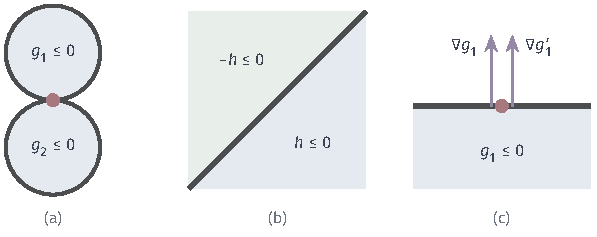
\includegraphics[width=101mm]{figures/05-optimization/06-constrained-optimization/tikz/nlipm-no-interior/figure.pdf}
  \caption{内点法的条件在模型层面失效的三种情形。(a)两个相切的圆盘（浅蓝），可行集只有红点，没有内部。(b)$h\leq0$和$-h\leq0$的公共部分是深灰的直线，同样没有内部。(c)同一条约束写了两遍，紫色箭头是两个相同的梯度，它们线性相关，乘子不唯一。}
  \label{fig:nlipm-no-interior}
\end{BookInlineFigure}

\subsection{停止条件}
\label{sec:nlipm-stopping}

迭代点永远在内部，算法只能在某处停下。这一小节回答什么量决定停止，以及停下的点能保证什么。

\paragraph{三项分别评价}
对参数$\mu$，定义误差
\begin{equation}
 E_\mu(\bm{z})=\max\Bigl\{\frac{\lVert\bm{r}_{\mathrm{d}}\rVert_\infty}{c_{\mathrm{d}}},\ \lVert\bm{r}_{\mathrm{e}}\rVert_\infty,\ \lVert\bm{r}_{\mathrm{p}}\rVert_\infty,\ \frac{\lVert\bm{S}\bm{\Lambda}\bm{1}-\mu\bm{1}\rVert_\infty}{c_{\mathrm{c}}}\Bigr\},
 \label{eq:nlipm-error}
\end{equation}
这里$c_{\mathrm{d}},c_{\mathrm{c}}\geq1$是按乘子大小确定的缩放，防止乘子很大时要求过严，贯穿例中都取$1$。$E_\mu$度量子问题的误差，$E_0$才度量原问题的KKT误差。最后的判据是$E_0\leq\varepsilon$。

\paragraph{参数小不等于解好了}
一个很小的$\mu$什么都说明不了，因为$\mu$是算法自己设定的数。起点取$\bm{\lambda}=10^{-3}\bm{1}$，$\mu$立刻就很小，而$\bm{r}_{\mathrm{d}}$的大小是$2$。反过来，$E_\mu$很小也只说明子问题解得好。

图~\ref{fig:nlipm-stop-staircase}是贯穿例上的一次运行，每当$E_\mu\leq0.1\mu$时，令$\mu\leftarrow0.2\mu$。第$6$轮$E_\mu\approx1.3\times10^{-5}$，子问题已经解得很准，而$E_0=0.04$，正好是当时的$\mu$。可以看到$E_0$紧贴$\mu$下降，$E_\mu$每次更新参数后跳起，再快速下降。

\begin{BookInlineFigure}
  \centering
  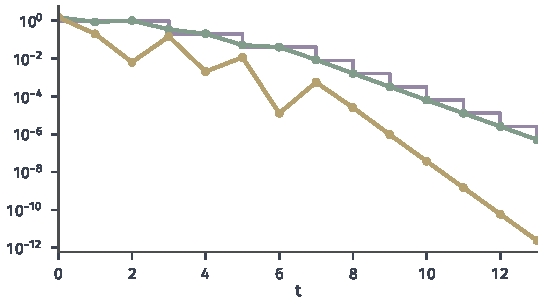
\includegraphics[width=92mm]{figures/05-optimization/06-constrained-optimization/matplotlib/nlipm-stop-staircase/figure.pdf}
  \caption{子问题误差与原问题误差，贯穿例，$\mu$只在$E_\mu\leq0.1\mu$时按$0.2$倍减小，对数纵轴。紫色折线是当前的$\mu$，绿线是原问题的KKT误差$E_0$，黄线是子问题误差$E_\mu$。$E_\mu$很小的时候，$E_0$仍然停在$\mu$的水平上。}
  \label{fig:nlipm-stop-staircase}
\end{BookInlineFigure}

\paragraph{内层精度与外层参数的配合}
由定义，$\lvert E_0-E_\mu\rvert\leq\mu/c_{\mathrm{c}}$，所以把$E_\mu$解得比$\mu$小很多并没有好处，$E_0$反正停在$\mu$的量级。常用的规则是：内层解到$E_\mu\leq\kappa\mu$，再更新参数
\begin{equation}
 \mu^+=\max\Bigl\{\frac{\varepsilon}{10},\ \min\bigl\{\tau\mu,\ \mu^{1+\theta}\bigr\}\Bigr\},
 \label{eq:nlipm-mu-update}
\end{equation}
其中$\kappa>0$，$\tau\in(0,1)$，$\theta\in(0,1)$。$\mu$大时线性减小，$\mu$小时超线性减小。下限$\varepsilon/10$防止参数比容差小太多，否则$\bm{D}$的数值徒然变大，矩阵更病态，而精度并不提高。

\paragraph{近似点能保证什么}
下面的定理说明残差小怎样转化成目标误差，它把定理~\ref{thm:nlipm-gap}推广到迭代点不在路径上、残差不为零的情形。

\begin{theorem}[近似点的目标误差]
\label{thm:nlipm-approx-certificate}
设$f$、$g_i$凸且可微，$\bm{h}(\bm{x})=\bm{A}\bm{x}-\bm{b}$，$(\bm{x},\bm{s},\bm{\lambda},\bm{\nu})$满足$\bm{\lambda}\geq\bm{0}$，残差如式~\eqref{eq:nlipm-residuals}定义。设$\bm{x}^\star$是最优解，$R\geq\lVert\bm{x}-\bm{x}^\star\rVert_2$。则
\begin{equation}
 f(\bm{x})-f^\star\leq\bm{\lambda}^\top\bm{s}-\bm{\lambda}^\top\bm{r}_{\mathrm{p}}-\bm{\nu}^\top\bm{r}_{\mathrm{e}}+\lVert\bm{r}_{\mathrm{d}}\rVert_2R.
 \label{eq:nlipm-approx-upper}
\end{equation}
若$(\bm{\lambda}^\star,\bm{\nu}^\star)$是一组KKT乘子，则还有
\begin{equation}
 f(\bm{x})-f^\star\geq-(\bm{\lambda}^\star)^\top\bm{g}(\bm{x})-(\bm{\nu}^\star)^\top\bm{r}_{\mathrm{e}}.
 \label{eq:nlipm-approx-lower}
\end{equation}
\end{theorem}

\begin{proof}
由$\bm{\lambda}\geq\bm{0}$和$\bm{x}^\star$可行，有
\[
 f^\star\geq\mathcal{L}(\bm{x}^\star,\bm{\lambda},\bm{\nu}).
\]
函数$\mathcal{L}(\cdot,\bm{\lambda},\bm{\nu})$是凸的，在$\bm{x}$处的梯度是$\bm{r}_{\mathrm{d}}$，于是
\[
 \mathcal{L}(\bm{x}^\star,\bm{\lambda},\bm{\nu})\geq\mathcal{L}(\bm{x},\bm{\lambda},\bm{\nu})+\bm{r}_{\mathrm{d}}^\top(\bm{x}^\star-\bm{x})\geq\mathcal{L}(\bm{x},\bm{\lambda},\bm{\nu})-\lVert\bm{r}_{\mathrm{d}}\rVert_2R.
\]
代入$\bm{g}(\bm{x})=\bm{r}_{\mathrm{p}}-\bm{s}$和$\bm{h}(\bm{x})=\bm{r}_{\mathrm{e}}$，$\mathcal{L}(\bm{x},\bm{\lambda},\bm{\nu})$展开为
\[
 f(\bm{x})-\bm{\lambda}^\top\bm{s}+\bm{\lambda}^\top\bm{r}_{\mathrm{p}}+\bm{\nu}^\top\bm{r}_{\mathrm{e}}.
\]
整理即得式~\eqref{eq:nlipm-approx-upper}。

对下界，$\bm{x}^\star$是凸函数$\mathcal{L}(\cdot,\bm{\lambda}^\star,\bm{\nu}^\star)$的最小点，并且由互补，这个最小值等于$f^\star$，于是
\[
 f^\star\leq\mathcal{L}(\bm{x},\bm{\lambda}^\star,\bm{\nu}^\star)=f(\bm{x})+(\bm{\lambda}^\star)^\top\bm{g}(\bm{x})+(\bm{\nu}^\star)^\top\bm{h}(\bm{x}).
\]
移项即得式~\eqref{eq:nlipm-approx-lower}。
\end{proof}

式~\eqref{eq:nlipm-approx-upper}右端的第一项是互补量，其余三项是残差被乘子和距离放大的部分。这正是第~\ref{chap:lp-interior-point}章不可行点上间隙公式的非线性版本。下界说明，点略微不可行时目标可以低于$f^\star$，低的幅度由违反量乘以最优乘子决定。

用表~\ref{tab:nlipm-run}中$t=4$的点核对。这时互补量和两个残差项是
\[
 \bm{\lambda}^\top\bm{s}\approx3.82\times10^{-3},\quad\lvert\bm{\lambda}^\top\bm{r}_{\mathrm{p}}\rvert\approx8.9\times10^{-6},\quad\lVert\bm{r}_{\mathrm{d}}\rVert_2\approx2.5\times10^{-5}.
\]
可行集的直径不超过$4.5$，取$R=4.5$，上界约为$3.92\times10^{-3}$。实际误差是$1.92\times10^{-3}$，确实在界内。

\paragraph{始终按原问题报告}
内点法的内部变量经过松弛、缩放，矩阵可能经过正则化，交付时都要回到原问题上算一遍。可行性按$\max_i\max\{g_i(\bm{x}),0\}$和$\lVert\bm{h}(\bm{x})\rVert_\infty$计算，而不是$\lVert\bm{r}_{\mathrm{p}}\rVert_\infty$，因为$s_i>0$时残差小并不排除$g_i(\bm{x})$略大于零。互补按$\lambda_i\lvert g_i(\bm{x})\rvert$计算，驻定按未缩放的梯度计算。

三种常见的修改都可能制造假象。矩阵正则化只改变方向，不改变残差的定义，所以它本身不影响判据，但$\delta_{\mathrm{c}}$较大时迭代可能停在一个并不满足等式的点上。把约束放宽成$g_i\leq\epsilon$的实现，要说明放宽量。恢复步骤之后乘子往往被重置，这时要用新的乘子重新计算$\bm{r}_{\mathrm{d}}$，不能沿用恢复之前的数值。

收敛到一个$E_0$很小的点，在非凸问题上也只说明这一点近似满足KKT条件。若需要二阶信息，还要看最后一次分解时是否用过$\delta_{\mathrm{w}}>0$，用过说明约化Hessian在该点并不正定。

\section{锥规划中的障碍}
\label{sec:nlipm-conic}

有些约束写成标量不等式并不自然。$\lVert\bm{u}\rVert_2\leq t$在$\bm{u}=\bm{0}$处不可微，矩阵正定更是一个无法用有限条光滑不等式简单表达的条件。接下来要弄清：怎样为这些集合直接造一个障碍，路径跟踪的哪些操作可以照搬，哪些不能？

\paragraph{共同的框架}
第~\ref{chap:quadratic-conic-programming}章的锥规划写成
\begin{equation}
 \min_{\bm{x}}\ \langle\bm{c},\bm{x}\rangle\quad\text{s.t.}\quad\mathcal{A}\bm{x}=\bm{b},\quad\bm{x}\in\bm{K},
 \label{eq:nlipm-conic-primal}
\end{equation}
其中$\bm{K}$是闭凸锥，$\mathcal{A}$是线性映射。它的对偶问题是
\begin{equation}
 \max_{\bm{y},\bm{z}}\ \bm{b}^\top\bm{y}\quad\text{s.t.}\quad\mathcal{A}^*\bm{y}+\bm{z}=\bm{c},\quad\bm{z}\in\bm{K}^*,
 \label{eq:nlipm-conic-dual}
\end{equation}
$\bm{K}^*$是对偶锥，$\mathcal{A}^*$是$\mathcal{A}$的伴随映射，$\bm{z}$的角色就是第~\ref{chap:lp-interior-point}章的对偶松弛。可行点上目标差仍是$\langle\bm{x},\bm{z}\rangle$。

设$\phi$是定义在$\bm{K}$内部的障碍函数。障碍问题$\min\langle\bm{c},\bm{x}\rangle+\mu\phi(\bm{x})$的一阶条件给出$\bm{c}+\mu\nabla\phi(\bm{x})=\mathcal{A}^*\bm{y}$。令$\bm{z}=\bm{c}-\mathcal{A}^*\bm{y}$，得到中心路径的方程
\begin{equation}
 \mathcal{A}\bm{x}=\bm{b},\qquad\mathcal{A}^*\bm{y}+\bm{z}=\bm{c},\qquad\bm{z}=-\mu\nabla\phi(\bm{x}).
 \label{eq:nlipm-conic-central}
\end{equation}
第三式就是互补方程的一般形式。取$\phi=-\sum_i\log x_i$，它就是$x_iz_i=\mu$。

间隙由障碍的一个性质决定。设$\phi$满足$\phi(\tau\bm{x})=\phi(\bm{x})-\vartheta\log\tau$，对所有$\tau>0$成立。对$\tau$求导再令$\tau=1$，得到
\[
 \langle\nabla\phi(\bm{x}),\bm{x}\rangle=-\vartheta.
\]
代入式~\eqref{eq:nlipm-conic-central}，沿路径的间隙是
\begin{equation}
 \langle\bm{x},\bm{z}\rangle=\vartheta\mu.
 \label{eq:nlipm-conic-gap}
\end{equation}
数$\vartheta$称为\term{障碍参数}（barrier parameter），它取代了线性规划中的$n$和本章前面的$m$。

\subsection{二阶锥障碍}
\label{sec:nlipm-soc}

记$\bm{x}=(\bm{u},t)$，$\bm{u}\in\mathbb{R}^{q}$，$t\in\mathbb{R}$，第~\ref{chap:quadratic-conic-programming}章的二阶锥是$\{(\bm{u},t):\lVert\bm{u}\rVert_2\leq t\}$。它的内部由$t>\lVert\bm{u}\rVert_2$给出，等价于$t>0$且$t^2-\lVert\bm{u}\rVert_2^2>0$。

\begin{definition}[二阶锥障碍]
\label{def:nlipm-soc-barrier}
记$\bm{R}=\operatorname{diag}(-\bm{I}_q,1)$，$\omega(\bm{x})=\bm{x}^\top\bm{R}\bm{x}$。在二阶锥内部定义
\begin{equation}
 \phi(\bm{x})=-\log\omega(\bm{x})=-\log\bigl(t^2-\lVert\bm{u}\rVert_2^2\bigr).
 \label{eq:nlipm-soc-barrier}
\end{equation}
\end{definition}

点靠近锥面时$\omega\downarrow0$，$\phi\to+\infty$，一整张锥面只用一项对数表达。由$\omega(\tau\bm{x})=\tau^2\omega(\bm{x})$，这个障碍的参数是$\vartheta=2$，与维数$q$无关。

\paragraph{导数}
由$\nabla\omega=2\bm{R}\bm{x}$、$\nabla^2\omega=2\bm{R}$和复合函数法则，得到
\begin{equation}
 \nabla\phi(\bm{x})=-\frac{2\bm{R}\bm{x}}{\omega},\qquad
 \nabla^2\phi(\bm{x})=\frac{4\bm{R}\bm{x}\bm{x}^\top\bm{R}}{\omega^2}-\frac{2\bm{R}}{\omega}.
 \label{eq:nlipm-soc-derivatives}
\end{equation}
$\bm{R}$不定，所以第二项不定，正定性要靠两项配合。

\begin{lemma}[二阶锥障碍的Hessian正定]
\label{lem:nlipm-soc-pd}
在二阶锥内部，$\nabla^2\phi(\bm{x})\succ\bm{0}$。
\end{lemma}

\begin{proof}
取非零的$\bm{d}=(\bm{v},r)$。考察二次函数
\[
 p(\beta)=(\bm{d}+\beta\bm{x})^\top\bm{R}(\bm{d}+\beta\bm{x})=\omega\beta^2+2\beta\,\bm{x}^\top\bm{R}\bm{d}+\bm{d}^\top\bm{R}\bm{d}.
\]
取$\beta_0=-r/t$，向量$\bm{d}+\beta_0\bm{x}$的最后一个分量为零，所以
\[
 p(\beta_0)=-\lVert\bm{v}+\beta_0\bm{u}\rVert_2^2\leq0.
\]
又$\omega>0$，所以$p$有实根，判别式非负，这就是
\[
 (\bm{x}^\top\bm{R}\bm{d})^2\geq\omega\,\bm{d}^\top\bm{R}\bm{d}.
\]

由式~\eqref{eq:nlipm-soc-derivatives}，Hessian的二次型是
\[
 \bm{d}^\top\nabla^2\phi\bm{d}=\frac{4(\bm{x}^\top\bm{R}\bm{d})^2}{\omega^2}-\frac{2\bm{d}^\top\bm{R}\bm{d}}{\omega}.
\]
若$\bm{d}^\top\bm{R}\bm{d}>0$，代入判别式不等式，它不小于$2\bm{d}^\top\bm{R}\bm{d}/\omega>0$。

若$\bm{d}^\top\bm{R}\bm{d}\leq0$，两项都非负。两项同时为零时，$\bm{d}^\top\bm{R}\bm{d}=0$且$\bm{x}^\top\bm{R}\bm{d}=0$，于是
\[
 p(\beta)=\omega\beta^2.
\]
结合$p(\beta_0)\leq0$，得$\beta_0=0$，即$r=0$。这时$p(\beta_0)=0$给出$\bm{v}=\bm{0}$，与$\bm{d}\neq\bm{0}$矛盾。
\end{proof}

用一个二维的点核对，取$q=1$，$\bm{x}=(u,t)=(1,2)$，这时$\omega=3$。由式~\eqref{eq:nlipm-soc-derivatives}，
\[
 \nabla\phi=\begin{bmatrix}2/3\\-4/3\end{bmatrix},\qquad
 \nabla^2\phi=\frac19\begin{bmatrix}10&-8\\-8&10\end{bmatrix}.
\]
Hessian的特征值是$2/9$和$2$，都是正的。

\paragraph{允许的步长}
沿方向$\bm{d}=(\bm{v},r)$走到$\bm{x}+\alpha\bm{d}$，$\omega$是$\alpha$的二次函数：
\begin{equation}
 \omega(\alpha)=\omega+2\alpha\,\bm{x}^\top\bm{R}\bm{d}+\alpha^2\,\bm{d}^\top\bm{R}\bm{d}.
 \label{eq:nlipm-soc-step}
\end{equation}
$\alpha_{\max}$是使$t+\alpha r>0$的前提下$\omega(\alpha)$的最小正根。这和线性规划的比值检验是同一件事，只是一次方程换成了二次方程，仍然有精确的公式，不需要试探。

例中取$\bm{d}=(2,-1)$，式~\eqref{eq:nlipm-soc-step}给出
\[
 \omega(\alpha)=3-8\alpha-3\alpha^2=(1-3\alpha)(3+\alpha).
\]
最小正根是$\alpha_{\max}=1/3$，对应锥面上的点$(5/3,5/3)$。沿这条线，$\phi$的两个导数是$8/3$和$82/9$，图~\ref{fig:nlipm-soc-barrier}(b)的黄线就是这个二次模型，它在边界处仍是有限值，真正的障碍趋于无穷。

\begin{BookInlineFigure}
  \centering
  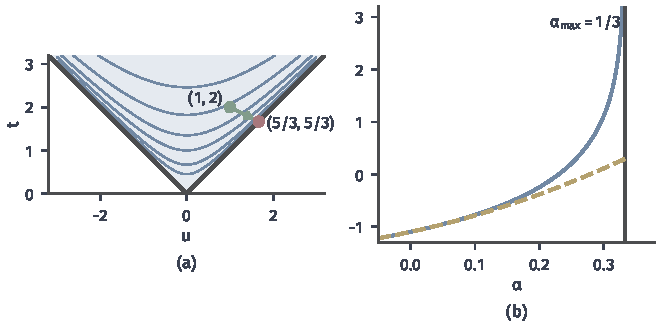
\includegraphics[width=112mm]{figures/05-optimization/06-constrained-optimization/matplotlib/nlipm-soc-barrier/figure.pdf}
  \caption{二阶锥（$q=1$）的障碍。(a)浅蓝区域是锥内部，深灰粗线是锥面，蓝线是$\phi$的等值线。绿点是$(1,2)$，绿色箭头是方向$(2,-1)$，红点是它到达锥面的位置$(5/3,5/3)$。(b)沿该方向的$\phi$（蓝线）与它在$\alpha=0$处的二次模型（黄色虚线），深灰粗线是$\alpha_{\max}=1/3$。}
  \label{fig:nlipm-soc-barrier}
\end{BookInlineFigure}

\paragraph{仿射映射进入锥后的Newton系统}
实际问题的约束通常写成
\[
 \lVert\bm{B}\bm{x}+\bm{e}\rVert_2\leq\bm{a}^\top\bm{x}+d,
\]
也就是$\bm{y}(\bm{x})=\bm{Q}\bm{x}+\bm{q}$落在锥中，这里$\bm{Q}$由$\bm{B}$和$\bm{a}^\top$拼成，$\bm{q}=(\bm{e},d)$。由链式法则，
\begin{equation}
 \nabla_{\bm{x}}\phi=\bm{Q}^\top\nabla\phi(\bm{y}),\qquad
 \nabla_{\bm{x}}^2\phi=\bm{Q}^\top\nabla^2\phi(\bm{y})\bm{Q}.
 \label{eq:nlipm-soc-affine}
\end{equation}

把式~\eqref{eq:nlipm-soc-derivatives}代入，得到的矩阵是“稀疏的$\bm{Q}^\top\bm{R}\bm{Q}$”加上一个秩一矩阵。秩一项的向量$\bm{Q}^\top\bm{R}\bm{y}$通常是稠密的，直接相加会填满矩阵。保留锥结构的实现把它单独存放，或者在鞍点矩阵中增加一行一列，这样既不丢失稀疏性，也能用现成的分解。

\paragraph{展开成标量约束的代价}
也可以把约束写成标量不等式$g(\bm{u},t)=\lVert\bm{u}\rVert_2-t\leq0$，用本章前几节的方法。问题出在$\bm{u}=\bm{0}$：$g$在这里不可微，而这恰恰可能是解所在的位置，例如目标要把$\lVert\bm{B}\bm{x}+\bm{e}\rVert_2$压到零时。图~\ref{fig:nlipm-soc-kink}显示，$-\log(t-\lVert\bm{u}\rVert_2)$在$\bm{u}=\bm{0}$处有折角，$-\log(t^2-\lVert\bm{u}\rVert_2^2)$却是光滑的，因为它用平方把折角消掉了。

改写成$g=\lVert\bm{u}\rVert_2^2-t^2\leq0$并不解决问题。这个$g$不是凸函数，它的零下水平集还包括$t<0$的另一半锥，所以必须同时约束$t\geq0$。二阶锥障碍用$\omega$的同时把定义域限定在$t>0$的内部，避免了这两个麻烦。

\begin{BookInlineFigure}
  \centering
  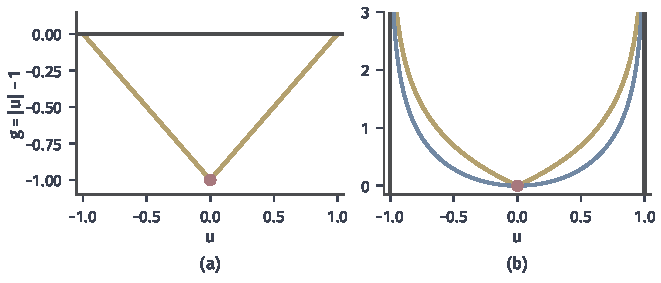
\includegraphics[width=112mm]{figures/05-optimization/06-constrained-optimization/matplotlib/nlipm-soc-kink/figure.pdf}
  \caption{标量写法与锥障碍，$t=1$。(a)标量约束$g=\lvert u\rvert-1$在$u=0$处有折角（红点）。(b)黄线是$-\log(1-\lvert u\rvert)$，保留了折角；蓝线是二阶锥障碍$-\log(1-u^2)$，在$u=0$处光滑。深灰粗线是边界。}
  \label{fig:nlipm-soc-kink}
\end{BookInlineFigure}

\subsection{半正定锥障碍}
\label{sec:nlipm-psd}

变量换成对称矩阵$\bm{X}\in\mathcal{S}^n$，约束是$\bm{X}\succeq\bm{0}$，内积是迹内积
\[
 \langle\bm{X},\bm{Z}\rangle=\operatorname{tr}(\bm{X}\bm{Z}).
\]
半正定锥在这个内积下是自对偶的，所以$\bm{K}^*=\bm{K}$。

\paragraph{特征值逼近零}
$\bm{X}$越靠近边界，最小的特征值越接近零。记$\bm{X}$的特征值为$\rho_1,\ldots,\rho_n>0$，对每个特征值都放一项对数障碍，得到
\begin{equation}
 \phi(\bm{X})=-\sum_{i=1}^n\log\rho_i(\bm{X})=-\log\det\bm{X}.
 \label{eq:nlipm-psd-barrier}
\end{equation}
计算时不必求特征值，$\log\det$可以由Cholesky分解得到。由$\det(\tau\bm{X})=\tau^n\det\bm{X}$，障碍参数是$\vartheta=n$。

\paragraph{线性扰动下的导数}
沿对称方向$\bm{D}$看。因为$\bm{X}\succ\bm{0}$，可以写成
\[
 \bm{X}+\alpha\bm{D}=\bm{X}^{1/2}\bigl(\bm{I}+\alpha\bm{X}^{-1/2}\bm{D}\bm{X}^{-1/2}\bigr)\bm{X}^{1/2}.
\]
记$\bm{X}^{-1/2}\bm{D}\bm{X}^{-1/2}$的特征值为$\beta_1,\ldots,\beta_n$，它们也是$\bm{X}^{-1}\bm{D}$的特征值。取行列式再取对数，得到
\begin{equation}
 \phi(\bm{X}+\alpha\bm{D})=\phi(\bm{X})-\sum_{i=1}^n\log(1+\alpha\beta_i).
 \label{eq:nlipm-psd-expansion}
\end{equation}
对$\alpha$展开到二阶，一阶系数是$-\sum_i\beta_i$，二阶系数是$\sum_i\beta_i^2$。写成迹，就是
\begin{equation}
 \begin{gathered}
 \langle\nabla\phi(\bm{X}),\bm{D}\rangle=-\operatorname{tr}(\bm{X}^{-1}\bm{D}),\\
 \langle\bm{D},\nabla^2\phi(\bm{X})[\bm{D}]\rangle=\operatorname{tr}(\bm{X}^{-1}\bm{D}\bm{X}^{-1}\bm{D}).
 \end{gathered}
 \label{eq:nlipm-psd-derivatives}
\end{equation}
所以在迹内积下$\nabla\phi(\bm{X})=-\bm{X}^{-1}$，Hessian是线性算子$\bm{D}\mapsto\bm{X}^{-1}\bm{D}\bm{X}^{-1}$。

式~\eqref{eq:nlipm-psd-expansion}同时给出最大步长。$\bm{X}+\alpha\bm{D}\succ\bm{0}$当且仅当每个$1+\alpha\beta_i>0$，所以若$\beta_{\min}<0$，
\begin{equation}
 \alpha_{\max}=-\frac{1}{\beta_{\min}},
 \label{eq:nlipm-psd-step}
\end{equation}
否则$\alpha_{\max}=+\infty$。

用具体的矩阵算一遍。取
\[
 \bm{X}=\begin{bmatrix}2&1\\1&2\end{bmatrix},\qquad\bm{D}=\begin{bmatrix}-1&-1\\-1&-2\end{bmatrix}.
\]
$\bm{X}$的特征值是$1$和$3$。直接计算，
\[
 \bm{X}^{-1}\bm{D}=\frac13\begin{bmatrix}-1&0\\-1&-3\end{bmatrix},
\]
它的特征值是$-1/3$和$-1$，所以$\alpha_{\max}=1$。可以核对，$\bm{X}+\bm{D}$的第二行是零，确实落在边界上。

由式~\eqref{eq:nlipm-psd-derivatives}，一阶、二阶导数分别是
\[
 \frac13+1=\frac43,\qquad\frac19+1=\frac{10}{9}.
\]
而$\det(\bm{X}+\alpha\bm{D})=(1-\alpha)(3-\alpha)$，对$-\log$直接求导得到同样的数。图~\ref{fig:nlipm-psd-barrier}显示了特征值沿这个方向的变化和障碍的上升。

\begin{BookInlineFigure}
  \centering
  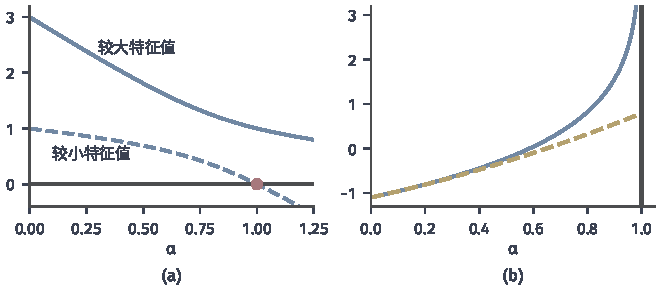
\includegraphics[width=112mm]{figures/05-optimization/06-constrained-optimization/matplotlib/nlipm-psd-barrier/figure.pdf}
  \caption{半正定锥的障碍，沿$\bm{X}+\alpha\bm{D}$。(a)$\bm{X}+\alpha\bm{D}$的两个特征值，红点是较小的特征值到达零的位置$\alpha_{\max}=1$，深灰粗线是零。(b)蓝线是$-\log\det(\bm{X}+\alpha\bm{D})$，黄色虚线是它在$\alpha=0$处的二次模型，深灰粗线是$\alpha_{\max}$。}
  \label{fig:nlipm-psd-barrier}
\end{BookInlineFigure}

\paragraph{矩阵的互补不能照搬标量操作}
中心路径的第三式是$\bm{Z}=\mu\bm{X}^{-1}$，等价于$\bm{X}\bm{Z}=\mu\bm{I}$。标量情形下，线性化$x_is_i=\mu$毫无歧义。矩阵情形下，直接线性化得到
\begin{equation}
 \Delta\bm{X}\,\bm{Z}+\bm{X}\Delta\bm{Z}=\sigma\mu\bm{I}-\bm{X}\bm{Z}.
 \label{eq:nlipm-psd-linearize}
\end{equation}
麻烦在于$\bm{X}$和$\bm{Z}$不交换，$\bm{X}\bm{Z}$一般不对称。解出来的$\Delta\bm{X}$也不对称，走一步之后$\bm{X}$就离开了对称矩阵空间。

看一个具体的例子。取前面的$\bm{X}$，再取$\bm{Z}=\operatorname{diag}(1,2)$，对偶方向$\Delta\bm{Z}$是非对角的对称矩阵。由式~\eqref{eq:nlipm-psd-linearize}解$\Delta\bm{X}$时，出现的项是
\[
 \bm{X}\Delta\bm{Z}\bm{Z}^{-1}=\begin{bmatrix}2&1\\1&2\end{bmatrix}\begin{bmatrix}0&1\\1&0\end{bmatrix}\begin{bmatrix}1&0\\0&1/2\end{bmatrix}=\begin{bmatrix}1&1\\2&1/2\end{bmatrix},
\]
它不是对称的。

解决的办法是\term{原始—对偶缩放}（primal-dual scaling）：选一个可逆矩阵$\bm{P}$，不线性化$\bm{X}\bm{Z}$，而线性化对称化之后的量
\begin{equation}
 \mathcal{H}_{\bm{P}}(\bm{M})=\tfrac12\bigl(\bm{P}\bm{M}\bm{P}^{-1}+(\bm{P}\bm{M}\bm{P}^{-1})^\top\bigr),\qquad
 \mathcal{H}_{\bm{P}}(\bm{X}\bm{Z})=\mu\bm{I}.
 \label{eq:nlipm-psd-scaling}
\end{equation}
三种选择最常见：$\bm{P}=\bm{I}$只把结果对称化；$\bm{P}=\bm{Z}^{1/2}$称为HKM方向；$\bm{P}$取Nesterov—Todd缩放矩阵时，$\bm{X}$与$\bm{Z}$被映到同一个矩阵。不同选择的方向不同，都要保证$\Delta\bm{X}$、$\Delta\bm{Z}$是对称的。

以HKM方向为例，把$\Delta\bm{X}$对称化之后，得到
\[
 \Delta\bm{X}=\sigma\mu\bm{Z}^{-1}-\bm{X}-\tfrac12\bigl(\bm{X}\Delta\bm{Z}\bm{Z}^{-1}+\bm{Z}^{-1}\Delta\bm{Z}\bm{X}\bigr).
\]
代入约束，形成关于$\Delta\bm{y}$的方程，系数矩阵的元素是
\begin{equation}
 M_{ij}=\operatorname{tr}\bigl(\bm{A}_i\bm{X}\bm{A}_j\bm{Z}^{-1}\bigr),
 \label{eq:nlipm-psd-schur}
\end{equation}
其中$\bm{A}_i$是约束$\langle\bm{A}_i,\bm{X}\rangle=b_i$的系数矩阵。它是第~\ref{chap:lp-interior-point}章$\bm{A}\bm{D}\bm{A}^\top$的矩阵版本。

\paragraph{内积配对要保持一致}
实现中常把对称矩阵排成向量，这一步很容易出错。$\bm{X}$有$n(n+1)/2$个独立元素，若直接取上三角排成向量，内积就变了。前面的$\bm{X}$满足$\operatorname{tr}(\bm{X}^2)=10$，而向量$(2,1,2)$的平方和是$9$，因为非对角元在迹里算了两次。

正确的做法是把非对角元乘以$\sqrt{2}$，得到$(2,\sqrt{2},2)$，平方和正好是$10$。对偶变量、梯度和$\mathcal{A}^*$都要用同样的约定，否则对偶可行性和间隙算的都不是原来的量。

\paragraph{三种障碍的对比}
表~\ref{tab:nlipm-barriers}把本章的三种障碍放在一起。形式相同的地方是路径和间隙的公式，不同的地方在互补的写法和步长的求法，这两处决定了线性代数的结构。

\begin{BookInlineTable}
  \centering
  \footnotesize
  \begin{tabular}{@{}llll@{}}
    \toprule
    量 & 标量$s>0$ & 二阶锥 & 半正定锥\\
    \midrule
    障碍 & $-\log s$ & $-\log(t^2-\lVert\bm{u}\rVert_2^2)$ & $-\log\det\bm{X}$\\
    参数$\vartheta$ & $1$ & $2$ & $n$\\
    $-\nabla\phi$ & $1/s$ & $2\bm{R}\bm{x}/\omega$ & $\bm{X}^{-1}$\\
    内积 & 乘法 & 欧氏内积 & 迹内积\\
    $\alpha_{\max}$ & 比值 & 二次方程的根 & $\bm{X}^{-1}\bm{D}$的特征值\\
    线性代数 & 对角 & 对角加秩一 & 稠密缩放矩阵\\
    \bottomrule
  \end{tabular}
  \caption{三种锥的障碍及相应的计算。}
  \label{tab:nlipm-barriers}
\end{BookInlineTable}

\section{保证与计算成本}
\label{sec:nlipm-guarantees}

第~\ref{chap:lp-interior-point}章证明了线性规划上短步路径跟踪的迭代界。这就需要回答：这个结果在什么条件下能够推广，在什么情形下必须退回局部结论，以及每一轮实际要花多少计算？

\paragraph{为什么要有一个比光滑更强的条件}
Newton法的通常分析用Hessian的Lipschitz常数$M$，结论依赖坐标的选取。障碍函数在边界附近的三阶导数趋于无穷，$M$根本不存在一个有限的整体值。路径跟踪的分析需要一种随点变化的尺子。

用$\phi$自己的Hessian当尺子。下面的条件要求三阶导数被二阶导数控制，这就是\term{自协调}（self-concordant）。

\begin{definition}[自协调障碍]
\label{def:nlipm-self-concordant}
设$\phi$是开凸集上三阶连续可微的凸函数，在边界附近趋于$+\infty$。记$\phi'$、$\phi''$、$\phi'''$为沿方向$\bm{d}$的方向导数。若对所有点和所有方向，
\begin{equation}
 \lvert\phi'''\rvert\leq2(\phi'')^{3/2},\qquad(\phi')^2\leq\vartheta\,\phi'',
 \label{eq:nlipm-self-concordant}
\end{equation}
就称$\phi$是参数为$\vartheta$的自协调障碍。
\end{definition}

对$\phi(x)=-\log x$，沿$d=1$的三个导数是$-1/x$、$1/x^2$、$-2/x^3$。代入两个不等式，都恰好取等号，其中$\vartheta=1$。第一个不等式的两边在缩放$x$时变化相同，所以这个条件不依赖坐标的单位。

三种基本的障碍都是自协调的：$m$条线性约束的对数障碍参数是$m$，二阶锥障碍参数是$2$，$n\times n$半正定锥障碍参数是$n$。凸二次约束的$-\log(-g)$也是自协调的，参数是$1$，所以贯穿例的障碍参数是$\vartheta=2$。

\paragraph{Dikin椭球：局部模型信多远}
自协调的直接后果是，以$\nabla^2\phi$定义的单位椭球落在定义域内：
\begin{equation}
 \bigl\{\bm{x}+\bm{d}:\bm{d}^\top\nabla^2\phi(\bm{x})\bm{d}<1\bigr\}\subset\operatorname{dom}\phi.
 \label{eq:nlipm-dikin}
\end{equation}
这个集合称为\term{Dikin椭球}（Dikin ellipsoid）。多面体的情形可以直接验证：$\bm{g}(\bm{x})=\bm{A}\bm{x}-\bm{b}$时，二次型等于$\sum_i(\bm{a}_i^\top\bm{d}/s_i)^2$。它小于$1$，就有每个$\lvert\bm{a}_i^\top\bm{d}\rvert<s_i$，于是新点的每个松弛都还是正的。

一般情形的证明需要沿线段积分第一个不等式，读者可查阅专著\scite{math-boyd2004convex}。

图~\ref{fig:nlipm-dikin}画出贯穿例的四个Dikin椭球，在椭球边界上逐点计算，松弛都是正的。靠近边界时椭球在法向变扁，在切向仍然较长。这就是局部模型“信多远”的答案，随位置自动调整，不需要知道全局的光滑常数。

\begin{BookInlineFigure}
  \centering
  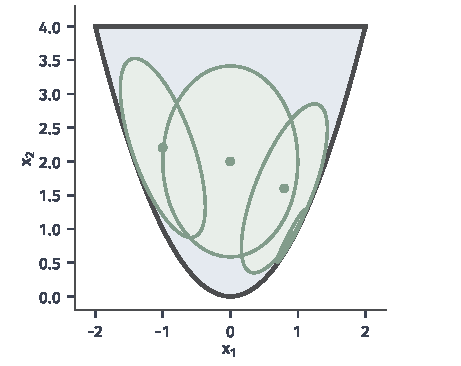
\includegraphics[width=78mm]{figures/05-optimization/06-constrained-optimization/matplotlib/nlipm-dikin/figure.pdf}
  \caption{贯穿例的Dikin椭球，绿点是四个基点，绿色曲线是$\bm{d}^\top\nabla^2\phi(\bm{x})\bm{d}=1$围成的椭球。四个椭球都留在可行集（浅蓝）之内，靠近边界的椭球更扁。}
  \label{fig:nlipm-dikin}
\end{BookInlineFigure}

\paragraph{凸问题的迭代界}
有了这把尺子，第~\ref{chap:lp-interior-point}章的短步分析可以整体推广，其中$\sqrt{n}$换成$\sqrt{\vartheta}$。结论如下，证明要用到自协调函数的Newton减量分析，篇幅较长，读者可查阅专著\scite{math-boyd2004convex}。

\begin{theorem}[路径跟踪的迭代次数]
\label{thm:nlipm-complexity}
设目标是线性函数，可行集有界且有严格可行点，$\phi$是参数为$\vartheta$的自协调障碍，起点足够靠近路径。则短步路径跟踪得到$\varepsilon$精度的解所需的Newton步数为
\begin{equation}
 O\Bigl(\sqrt{\vartheta}\,\log\frac{\vartheta\mu^{(0)}}{\varepsilon}\Bigr).
 \label{eq:nlipm-complexity}
\end{equation}
\end{theorem}

这个界不依赖$f$和$g_i$的条件数，只依赖$\vartheta$，这是内点法在凸问题上最强的结论。目标非线性时，可以用上图形式把它移进约束，代价是要为新的约束找到自协调障碍。

式~\eqref{eq:nlipm-complexity}也解释了为什么锥结构有价值。一个$q+1$维的二阶锥只贡献$\vartheta=2$，如果把它拆成很多线性不等式去逼近，$\vartheta$就随拆分的条数增长。

\paragraph{线性规划的结论不能外推}
多项式界依赖两件事：约束有容易计算的自协调障碍，并且问题是凸的。两者都可能不成立。

第一，凸性并不自动给出自协调。取$g(x)=\mathrm{e}^x-1\leq0$，障碍$\phi=-\log(1-\mathrm{e}^x)$是凸函数，但$x\to-\infty$时$\phi''$和$\phi'''$都约等于$\mathrm{e}^x$，于是
\[
 \frac{\lvert\phi'''\rvert}{(\phi'')^{3/2}}\approx\mathrm{e}^{-x/2}\to\infty.
\]
第一个不等式不可能成立。每个开凸集都存在参数为$O(n)$的自协调障碍，但这是存在性的结果，这样的障碍一般无法计算。

第二，非凸问题求全局解是NP难的，非凸二次规划就已经如此，所以不可能有类似式~\eqref{eq:nlipm-complexity}的全局结果，除非$\mathrm{P}=\mathrm{NP}$。

\paragraph{非凸问题的局部收敛}
非凸问题上能证明的是：在定理~\ref{thm:nlipm-local-path}的条件下，从足够近的点出发，Newton迭代跟着路径收敛到KKT点。下面给出一步的估计。记$\bm{z}^\star$为该KKT点及其松弛、乘子，$\bm{F}_\mu(\bm{z})=\bm{F}_0(\bm{z})-\mu\bm{e}$，其中$\bm{e}$只在互补方程处为$1$，$\bm{G}$是$\bm{F}_0$的Jacobian矩阵。

\begin{theorem}[Newton步的局部估计]
\label{thm:nlipm-local-rate}
设定理~\ref{thm:nlipm-local-path}的条件成立，$\nabla^2f$、$\nabla^2g_i$、$\nabla^2h_j$在$\bm{x}^\star$附近是$M$-Lipschitz的。则存在$\bm{z}^\star$的邻域和常数$C_{\mathrm{G}}$、$M_{\mathrm{G}}$、$C_{\mathrm{p}}$（$M_{\mathrm{G}}$由$M$和乘子的界决定），使邻域内的$\bm{z}$和足够小的$\mu^+>0$满足：单位Newton步
\begin{equation}
 \bm{z}^+=\bm{z}-\bm{G}(\bm{z})^{-1}\bm{F}_{\mu^+}(\bm{z})
 \label{eq:nlipm-local-step}
\end{equation}
有
\begin{equation}
 \lVert\bm{z}^+-\bm{z}^\star\rVert_2\leq\frac{C_{\mathrm{G}}M_{\mathrm{G}}}{2}\bigl(\lVert\bm{z}-\bm{z}^\star\rVert_2+C_{\mathrm{p}}\mu^+\bigr)^2+C_{\mathrm{p}}\mu^+.
 \label{eq:nlipm-local-rate}
\end{equation}
\end{theorem}

\begin{proof}
定理~\ref{thm:nlipm-local-path}的证明说明$\bm{G}(\bm{z}^\star)$非奇异，所以在邻域内
\[
 \lVert\bm{G}(\bm{z})^{-1}\rVert_2\leq C_{\mathrm{G}}.
\]
$\bm{G}$的各块由$\nabla f$、$\nabla^2f$、$\nabla^2g_i$、$\nabla^2h_j$和乘子组成，因此在邻域内是$M_{\mathrm{G}}$-Lipschitz的。路径连续可微，所以
\[
 \lVert\bm{z}(\mu)-\bm{z}^\star\rVert_2\leq C_{\mathrm{p}}\mu.
\]

记$\bm{z}'=\bm{z}(\mu^+)$，它满足$\bm{F}_{\mu^+}(\bm{z}')=\bm{0}$。由Newton步的定义，
\[
 \bm{z}^+-\bm{z}'=\bm{G}(\bm{z})^{-1}\Bigl[\bm{G}(\bm{z})(\bm{z}-\bm{z}')-\bigl(\bm{F}_{\mu^+}(\bm{z})-\bm{F}_{\mu^+}(\bm{z}')\bigr)\Bigr].
\]
方括号内是一阶Taylor余项，由$\bm{G}$的Lipschitz性，它的范数不超过$\tfrac12M_{\mathrm{G}}\lVert\bm{z}-\bm{z}'\rVert_2^2$。于是
\[
 \lVert\bm{z}^+-\bm{z}'\rVert_2\leq\tfrac12C_{\mathrm{G}}M_{\mathrm{G}}\lVert\bm{z}-\bm{z}'\rVert_2^2.
\]
由三角不等式，$\bm{z}$到$\bm{z}'$的距离满足
\[
 \lVert\bm{z}-\bm{z}'\rVert_2\leq\lVert\bm{z}-\bm{z}^\star\rVert_2+C_{\mathrm{p}}\mu^+.
\]
再对$\bm{z}^+$用一次三角不等式，即得结论。
\end{proof}

式~\eqref{eq:nlipm-local-rate}右端有两项：Newton法自身的二次项，以及目标参数的偏移。$\mu^+$与当前误差同阶时，收敛是线性的，表~\ref{tab:nlipm-run}中$\sigma$固定为$0.2$，误差每轮大约乘以$0.2$，就是这种情形。按式~\eqref{eq:nlipm-mu-update}让$\mu^+$超线性减小，收敛速度也变成超线性。

这个估计假设单位步可以走，定理本身没有保证这一点，还要证明$\alpha=1$满足比例规则：活动约束的$s_i$和不活动约束的$\lambda_i$都是$O(\mu)$量级的小量，方向也必须是相应量级，这需要参数更新不能太快，也需要$\eta\to1$。完整的论证较长，读者可查阅专著\scite{math-nocedal2006numerical}。

\paragraph{全局的情形}
从任意点出发，非凸问题上能证明的是：在迭代点有界、矩阵经过惯性修正、约束正则等假设下，带过滤器或合成目标检验的算法的极限点要么满足KKT条件，要么是约束违反量的驻点。这里没有全局最优的保证，图~\ref{fig:nlipm-nonconvex-fold}已经说明，路径本身可能走向较差的局部解。表~\ref{tab:nlipm-claims}总结了两类问题上结论的区别。

\begin{BookInlineTable}
  \centering
  \footnotesize
  \begin{tabular}{@{}lll@{}}
    \toprule
    问题 & 凸问题 & 一般非凸问题\\
    \midrule
    路径 & 整条存在且唯一 & 只在KKT点附近\\
    路径上的间隙 & $f-f^\star\leq m\mu$ & 无全局含义\\
    迭代界 & 自协调时$\sqrt{\vartheta}$型 & 无\\
    停止的含义 & 近似全局解的证书 & 近似KKT点\\
    不可行的判定 & 可给证书 & 只能报告局部驻点\\
    局部速度 & 超线性 & 正则性下超线性\\
    \bottomrule
  \end{tabular}
  \caption{内点法在凸问题与非凸问题上的结论。}
  \label{tab:nlipm-claims}
\end{BookInlineTable}

\paragraph{每一轮的代价}
一轮的工作分三块：计算$f$、$\bm{g}$、$\bm{h}$及其一二阶导数，分解线性系统，以及可能的回溯。回溯只重新计算函数值，比较便宜。决定性的是分解。

压缩矩阵$\tilde{\bm{H}}=\bm{W}+\bm{J}^\top\bm{D}\bm{J}$是$n\times n$的。若有一条约束涉及很多变量，$\bm{J}$有一个稠密的行，$\bm{J}^\top\bm{D}\bm{J}$就是稠密的。鞍点形式~\eqref{eq:nlipm-saddle}维数大，却保留了稀疏性。

图~\ref{fig:nlipm-sparse-fill}是一个$n=m=20$的算例，$\bm{J}$是双对角的，最后一行稠密，共$58$个非零元，取$\bm{W}=\bm{I}$。压缩矩阵完全稠密，它的下三角因子有$210$个非零元。$40\times40$的鞍点矩阵把稠密行排在最后，下三角因子只有$117$个非零元。

这和第~\ref{chap:lp-interior-point}章的$\bm{A}\bm{D}\bm{A}^\top$是同一个现象，只是这里还多了$\bm{W}$。稠密情形下，$n\times n$的分解需要约$n^3/3$次运算；鞍点矩阵不定，要用$\bm{L}\bm{D}\bm{L}^\top$分解和主元选择，主元顺序会随数值改变，符号分析不能像线性规划那样只做一次。每试一个$\delta_{\mathrm{w}}$就要重新分解一次。

\begin{BookInlineFigure}
  \centering
  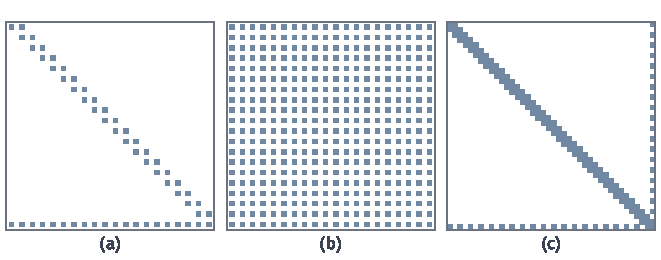
\includegraphics[width=112mm]{figures/05-optimization/06-constrained-optimization/matplotlib/nlipm-sparse-fill/figure.pdf}
  \caption{三个矩阵的非零模式，蓝点表示非零元。(a)$20\times20$的Jacobian矩阵，双对角加上一个稠密行。(b)压缩矩阵$\bm{W}+\bm{J}^\top\bm{D}\bm{J}$，完全稠密。(c)鞍点矩阵$[\bm{W},\bm{J}^\top;\bm{J},-\bm{D}^{-1}]$，变量与约束交错排列，稠密行排在最后。}
  \label{fig:nlipm-sparse-fill}
\end{BookInlineFigure}

\paragraph{条件数}
$\bm{D}$的对角元是$\lambda_i/s_i$。$\mu\to0$时，活动约束上它约为$(\lambda_i^\star)^2/\mu$，趋于无穷，不活动约束上它约为$\mu/(s_i^\star)^2$，趋于零，矩阵的条件数按$1/\mu$增长。

图~\ref{fig:nlipm-cond-growth}显示，贯穿例的压缩矩阵和鞍点矩阵都是如此，保留鞍点结构并不能消除这种病态，它的好处在稀疏性。这种病态的结构很特殊，向后稳定的直接分解能够得到足够准确的方向；迭代法就没有这样幸运，共轭梯度类的方法在$\mu$小时需要专门的预条件子。

\begin{BookInlineFigure}
  \centering
  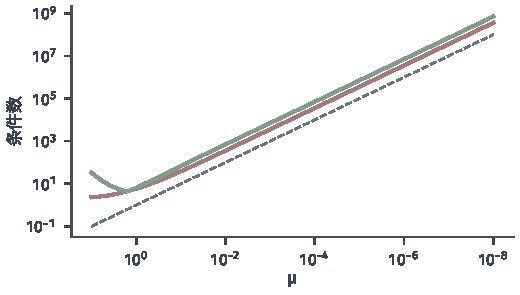
\includegraphics[width=88mm]{figures/05-optimization/06-constrained-optimization/matplotlib/nlipm-cond-growth/figure.pdf}
  \caption{贯穿例沿中心路径的条件数，横轴是$\mu$，向右减小。红线是压缩矩阵$\tilde{\bm{H}}$，绿线是鞍点矩阵，灰色虚线是参照线$1/\mu$。两条曲线都按$1/\mu$增长。}
  \label{fig:nlipm-cond-growth}
\end{BookInlineFigure}

\paragraph{外层轮数}
总代价等于外层轮数乘以每轮的分解代价。实际问题上，原始—对偶方法通常几十轮结束，这是经验而不是定理，它在式~\eqref{eq:nlipm-complexity}的界之下很多。

与第~\ref{chap:feasible-iterations}章的可行迭代和第~\ref{chap:penalty-multiplier-methods}章的乘子方法相比，内点法每轮的代价高，轮数少。能够精确分解时，内点法很有优势；分解太贵、只能得到低精度解就够时，一阶方法更合适。

\section{本章小结}
\label{sec:nlipm-summary}

本章开头的问题是，约束变弯之后，线性规划的路径跟踪还剩下什么。骨架都留下了：在不等式上加对数障碍，驻定条件给出扰动互补$s_i\lambda_i=\mu$，让$\mu$减小到零。等式约束没有内部，仍要显式保留。

新增的内容来自曲率。障碍的Hessian多了$\nabla^2g_i/(-g_i)$一项，Newton系统左上角多了Lagrange Hessian，松弛方程的残差不再按$1-\alpha$的比例下降。非凸时，矩阵可能在切空间上不正定，解方程得到的方向可能是上升方向，要靠惯性检查和矩阵正则化修正，再由残差检验或过滤器决定接受哪一步。

内部性、中心性和最优性是三种不同的检查对象。$\bm{s},\bm{\lambda}>\bm{0}$由到边界的比例规则维护，中心性由$\sigma$和邻域控制，最优性只能由驻定残差、约束残差和互补量共同判断。很小的$\mu$或很小的$E_\mu$都不是原问题的结论，最后要按未经修改的问题报告。

起点有两种。障碍路径需要严格可行点，可以用辅助问题求出；原始—对偶迭代只要求$\bm{s},\bm{\lambda}>\bm{0}$，可以从非零残差出发。没有严格内点、约束重复或线性相关时，问题出在模型上，需要单独检查。

二阶锥和半正定锥有各自的障碍$-\log(t^2-\lVert\bm{u}\rVert_2^2)$和$-\log\det\bm{X}$，路径和间隙的形式不变，$n$换成障碍参数$\vartheta$。步长由二次方程或特征值给出。矩阵互补不能照搬标量操作，$\Delta\bm{X}$要经缩放保持对称，内积配对也要前后一致。

能给出什么结论，由模型的条件决定。凸问题上有整条路径、间隙$m\mu$、近似点的误差界，自协调时还有$\sqrt{\vartheta}$型的迭代界。一般非凸问题只有KKT点附近的局部路径和局部收敛，路径可以断开，也可能通向较差的解，线性规划的多项式结论不能外推。

计算上，每轮的主要代价是分解Jacobian和Lagrange Hessian组成的鞍点矩阵。压缩形式维数小但可能稠密，鞍点形式保留稀疏性，两者的条件数都按$1/\mu$增长。


\chapter{流形优化}
\label{chap:manifold-optimization}

求一个对称矩阵的最小特征向量，可以写成单位球面上的极小化。本章全程使用下面这个三维小例子：
\begin{equation}
 \min_{\bm{x}\in\mathbb{R}^3}\ f(\bm{x})=\frac12\bm{x}^\top\bm{A}\bm{x}
 \quad\text{s.t.}\quad \bm{x}^\top\bm{x}=1,
 \qquad \bm{A}=\operatorname{diag}(1,2,4).
 \label{eq:mfo-running}
\end{equation}

$\bm{A}$是对角矩阵，答案一眼可见：极小点是$\pm\bm{e}_1$，最优值$f^\star=\tfrac12$。这样我们可以把注意力放在算法的每一步上，并随时核对结果。起点取
\[
 \bm{x}^{(0)}=\frac13(2,2,1)^\top,\qquad f(\bm{x}^{(0)})=\frac89.
\]

普通梯度步会马上碰到麻烦。图~\ref{fig:mfo-step-leaves}(a)中，沿切线方向走一步，点就飘到球面之外；图~\ref{fig:mfo-step-leaves}(b)中，矩阵的两列本来相互正交且长度为一，走一步后两列既不等长也不再正交。第~\ref{chap:feasible-iterations}章在圆周上用过局部消元再解方程恢复可行的办法，那里需要选基本变量，并在基矩阵病态时换基。

\begin{BookInlineFigure}
 \centering
 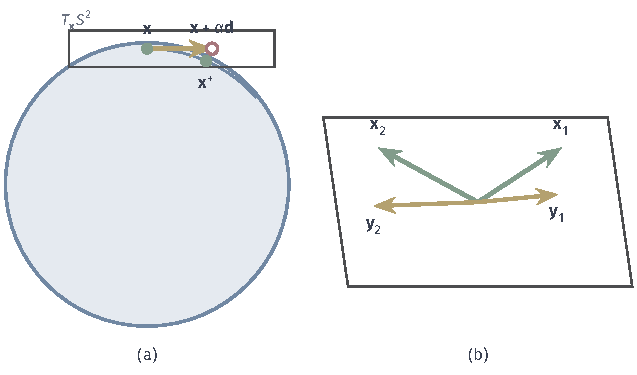
\includegraphics[width=107.9mm]{figures/05-optimization/06-constrained-optimization/tikz/mfo-step-leaves/figure.pdf}
 \caption{欧氏更新破坏光滑约束。(a)~浅蓝球面是可行集，方框是切平面的一块，黄箭头是切向的一步，红圈是落在球面外的点，虚线把它沿径向拉回到绿点。(b)~矩阵$\bm{X}$的两列$\bm{x}_1,\bm{x}_2$（绿）标准正交，方框是它们张成的平面；走一步后的两列$\bm{y}_1,\bm{y}_2$（黄）长度约为$1.094$和$1.144$，内积约为$0.247$，都离开了约束。}
 \label{fig:mfo-step-leaves}
\end{BookInlineFigure}

球面和正交矩阵的集合比一般的弯曲约束多一项便利：它们是光滑流形，而且切空间和回到集合上的运算都有便宜的公式。这一章的问题是：能否把这个集合本身当作计算空间，让迭代从头到尾都在集合上走，同时保留梯度法、Newton法、拟Newton法和信赖域的思路？

路线分三层。第~\ref{sec:mfo-problems}节和第~\ref{sec:mfo-optimality}节确定问题的形式和最优性条件，并算出切向梯度与切向曲率。第~\ref{sec:mfo-operations}节回答迭代缺少的三种运算：走完怎样回到集合上，怎样评价候选步，不同点处的向量怎样比较。

第~\ref{sec:mfo-first-order}节到第~\ref{sec:mfo-trust-region}节依次把这些运算装进一阶方法、二阶方法、拟Newton法和信赖域，每种方法都在上面的小例子上手算几步。第~\ref{sec:mfo-representation}节用子空间问题说明表示方式的影响，并在同一目标和同一精度下比较流形方法与一般约束方法。

\section{流形上的优化问题}
\label{sec:mfo-problems}

什么样的约束集合可以当作计算空间？本节先看两个具体约束，指出它们共有的结构，再说明这一结构在哪些集合上不存在。

\paragraph{两个具体约束}
球面约束$\bm{x}^\top\bm{x}=1$只有一个方程。从点$\bm{x}$出发沿曲线$\bm{c}(t)$运动，并一直留在球面上，就要求$\bm{c}(t)^\top\bm{c}(t)=1$。对$t$求导并取$t=0$，得到速度$\bm{v}=\bm{c}'(0)$必须满足
\[
 \bm{x}^\top\bm{v}=0.
\]
因此$\bm{x}$处允许的运动方向是与$\bm{x}$垂直的全体向量，构成一个$n-1$维的线性子空间。

矩阵约束$\bm{X}^\top\bm{X}=\bm{I}_k$的方程更多。这里$\bm{X}\in\mathbb{R}^{n\times k}$，$k\leq n$，它的列是一组标准正交向量。同样沿曲线$\bm{C}(t)$求导，速度$\bm{\Delta}=\bm{C}'(0)$必须满足
\[
 \bm{X}^\top\bm{\Delta}+\bm{\Delta}^\top\bm{X}=\bm{0}.
\]
这个条件说的是$\bm{X}^\top\bm{\Delta}$是反对称矩阵。例如$n=3$，$k=2$时，矩阵有$6$个元素，约束有$3$个独立方程，所以允许的方向构成一个$3$维子空间。

两个例子的共同点是：约束对变量的允许变化作出限制，而这个限制在每一点都是一个线性子空间，维数处处相同。这正是后面所有方法的立足点，在每一点都有一张平坦的“工作台”，可以在上面做线性代数。

\paragraph{正则等式约束给出流形}
把上面的观察写成一般形式。设$h:\mathbb{R}^n\to\mathbb{R}^p$光滑，可行集是它的零点集：
\begin{equation}
 M=\{\bm{x}\in\mathbb{R}^n:\ h(\bm{x})=\bm{0}\}.
 \label{eq:mfo-level-set}
\end{equation}
记$\bm{J}(\bm{x})$为$h$在$\bm{x}$处的Jacobian矩阵，假定它在$M$的每一点都行满秩。这就是第~\ref{chap:constrained-optimality}章的线性无关约束规范，这里要求它在整个可行集上成立。

这个条件保证$M$是$n-p$维的嵌入子流形，切空间就是Jacobian的零空间：
\begin{equation}
 T_{\bm{x}}M=\ker\bm{J}(\bm{x}).
 \label{eq:mfo-tangent}
\end{equation}
这里用到的是正则水平集定理及切空间的刻画，可参考\BookChapterRef{chap:manifold-relations}{卷四第26章“流形之间的关系”}。球面取$h(\bm{x})=\bm{x}^\top\bm{x}-1$，$\bm{J}(\bm{x})=2\bm{x}^\top$在球面上不为零；矩阵约束取值于对称矩阵，同样满足这个条件。

流形上的优化问题写作
\begin{equation}
 \min_{\bm{x}\in M}\ f(\bm{x}),
 \label{eq:mfo-problem}
\end{equation}
其中$f$定义在包含$M$的开集上并且光滑。本章把$M$就当作前面各章的可行集$\bm{C}$，并沿用卷四的写法把流形记成$M$，把球面记成$S^{n-1}$，把正交列矩阵的集合记成Stiefel流形$\mathrm{St}(k,n)$。问题本身仍是约束极值，改变的只是求解时使用的计算空间。

\paragraph{集合、度量与表示}
“在流形上计算”牵涉三个不同的选择，混淆它们会带来错误的结论。集合$M$由问题决定，它规定了哪些点可行，哪些点是极小点。

\term{黎曼度量}（Riemannian metric）是在每个切空间放一个内积，记为$\langle\bm{u},\bm{v}\rangle_{\bm{x}}$。同一个集合可以配不同的度量。度量决定长度和角度，因而决定“最陡”的方向，但不改变极小点的位置。本章除特别说明外，都取欧氏内积限制到切空间上的诱导度量。

表示方式是在计算机里怎样存一个点。球面上的点可以存成三个坐标，也可以存成两个角度；一个子空间可以存成任意一组基，这时同一个对象有许多矩阵记录。表示决定存储和运算的代价，第~\ref{sec:mfo-representation}节专门讨论。表~\ref{tab:mfo-three-choices}把三者并列。

\begin{BookInlineTable}
 \centering
 \caption{流形优化中三种不同的选择。}
 \label{tab:mfo-three-choices}
 \begin{tabular}{lll}
  \toprule
  选择 & 决定什么 & 不决定什么\\
  \midrule
  集合$M$ & 可行点、极小点 & 梯度的数值\\
  度量$\langle\cdot,\cdot\rangle_{\bm{x}}$ & 梯度、Hessian、步长的尺度 & 极小点的位置\\
  表示 & 存储和运算成本 & 所求的几何对象\\
  \bottomrule
 \end{tabular}
\end{BookInlineTable}

\paragraph{带奇点或棱角的集合}
前面的立足点并非总存在。图~\ref{fig:mfo-regular-singular}对比了三种集合。圆周上每点都有一条切线，法向量$\nabla h$不为零，这是正则的情形。

\begin{BookInlineFigure}
 \centering
 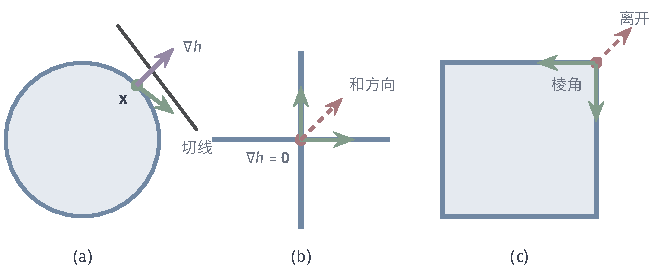
\includegraphics[width=111.9mm]{figures/05-optimization/06-constrained-optimization/tikz/mfo-regular-singular/figure.pdf}
 \caption{三种约束集合。(a)~圆周处处正则，切方向（绿）构成一条直线，紫箭头是约束的梯度。(b)~十字形$x_1x_2=0$在原点处约束梯度为零，两个绿色可行方向之和（红虚线）不可行，可行方向不构成线性子空间。(c)~正方形的角点处，可行方向只有一个锥，朝外的方向（红虚线）不可行。}
 \label{fig:mfo-regular-singular}
\end{BookInlineFigure}

十字形$\{x_1x_2=0\}$在原点处有两条可行的直线，把两个可行方向相加却得到不可行的方向，所以那里没有一个线性的切空间。这里$\nabla(x_1x_2)$在原点为零，正则条件不成立。

棱角的情形类似。方形可行域的角点处，允许的方向只构成一个锥，负向不再允许。这类可行集要用第~\ref{chap:feasible-iterations}章的投影或第~\ref{chap:penalty-multiplier-methods}章的乘子方法，本章的迭代不能直接套用，因为后面每一步都假定当前点处有一个完整的线性切空间。

\section{最优性与导数计算}
\label{sec:mfo-optimality}

普通的判据$\nabla f=\bm{0}$在球面上失效：在极小点$\bm{e}_1$处，$\nabla f$等于$\bm{e}_1$，并不为零。约束下应该把哪个量算成零，怎样判别二阶情形，这些量在具体约束上怎样计算？

\paragraph{切向梯度}
黎曼度量的作用之一是把微分变成向量：$\operatorname{grad}f(\bm{x})$是$T_{\bm{x}}M$中满足下式的唯一向量，$\mathrm{d}f_{\bm{x}}$是$f$在$\bm{x}$处的微分。
\begin{equation}
 \langle\operatorname{grad}f(\bm{x}),\bm{v}\rangle_{\bm{x}}=\mathrm{d}f_{\bm{x}}[\bm{v}],
 \qquad\forall\,\bm{v}\in T_{\bm{x}}M.
 \label{eq:mfo-riem-grad-def}
\end{equation}
这个向量称为\term{黎曼梯度}（Riemannian gradient）。微分和度量的具体定义见\BookChapterRef{chap:manifold-calculus}{卷四第28章“流形上的微积分”}，这里只用它的计算结果。

度量如何影响梯度？设切空间上的内积由对称正定矩阵$\bm{G}$给出，微分的系数向量记为$\bm{c}$。式~\eqref{eq:mfo-riem-grad-def}化成
\[
 \bm{v}^\top\bm{G}\operatorname{grad}f=\bm{v}^\top\bm{c},\qquad\forall\,\bm{v},
\]
于是
\[
 \operatorname{grad}f=\bm{G}^{-1}\bm{c}.
\]
取$\bm{c}=(1,1)^\top$做比较。$\bm{G}=\bm{I}$时梯度是$(1,1)^\top$；$\bm{G}=\operatorname{diag}(4,1)$时梯度是$(\tfrac14,1)^\top$。

图~\ref{fig:mfo-metric-gradient}解释这个差别。绿色区域是该度量下的单位球，梯度方向指向单位球上使线性函数最大的那一点。度量把单位球压扁，切点就移动了。两种度量下，梯度为零的条件都是$\bm{c}=\bm{0}$，所以驻点不受影响。

\begin{BookInlineFigure}
 \centering
 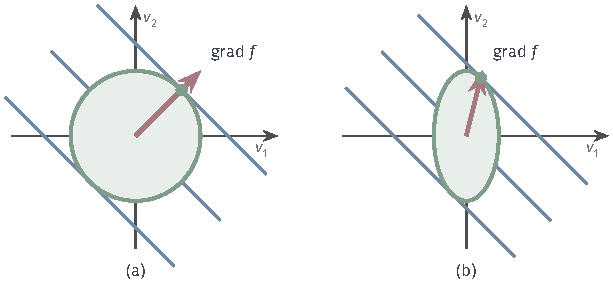
\includegraphics[width=103.8mm]{figures/05-optimization/06-constrained-optimization/tikz/mfo-metric-gradient/figure.pdf}
 \caption{同一微分在两种度量下的梯度。蓝线是线性函数$\mathrm{d}f[\bm{v}]=v_1+v_2$的等值线，绿色区域是度量的单位球，绿点是单位球上函数值最大的点，红箭头是梯度。(a)~$\bm{G}=\bm{I}$。(b)~$\bm{G}=\operatorname{diag}(4,1)$，单位球沿$v_1$被压缩，梯度偏向$v_2$。}
 \label{fig:mfo-metric-gradient}
\end{BookInlineFigure}

\paragraph{诱导度量下用投影计算}
取诱导度量时，黎曼梯度有一个直接的算法。设$\bar{f}$是$f$在环境空间中的光滑延拓，$\bm{P}_{\bm{x}}$是到$T_{\bm{x}}M$的正交投影。下面的引理说明，只要把欧氏梯度投影一下。

\begin{lemma}[投影公式]
 \label{lem:mfo-projection-gradient}
 设$M\subseteq\mathbb{R}^n$是嵌入子流形，取诱导度量，$\bar{f}$在$M$的邻域内光滑且在$M$上等于$f$。则
 \begin{equation}
  \operatorname{grad}f(\bm{x})=\bm{P}_{\bm{x}}\nabla\bar{f}(\bm{x}).
  \label{eq:mfo-projection-gradient}
 \end{equation}
\end{lemma}

\begin{proof}
 对$\bm{v}\in T_{\bm{x}}M$，取$M$上的曲线$\bm{c}$，满足$\bm{c}(0)=\bm{x}$，$\bm{c}'(0)=\bm{v}$。因为$f$与$\bar{f}$在$M$上相等，
 \[
  \mathrm{d}f_{\bm{x}}[\bm{v}]=\frac{\mathrm{d}}{\mathrm{d}t}\bar{f}(\bm{c}(t))\Big|_{t=0}=\langle\nabla\bar{f}(\bm{x}),\bm{v}\rangle.
 \]

 $\bm{P}_{\bm{x}}$是正交投影，$\bm{v}$在切空间中，所以$\bm{P}_{\bm{x}}\bm{v}=\bm{v}$，并且投影对称，于是
 \[
  \langle\nabla\bar{f}(\bm{x}),\bm{v}\rangle=\langle\nabla\bar{f}(\bm{x}),\bm{P}_{\bm{x}}\bm{v}\rangle=\langle\bm{P}_{\bm{x}}\nabla\bar{f}(\bm{x}),\bm{v}\rangle.
 \]
 $\bm{P}_{\bm{x}}\nabla\bar{f}(\bm{x})$在切空间中，又满足定义式~\eqref{eq:mfo-riem-grad-def}，由唯一性得结论。
\end{proof}

投影公式的适用条件是诱导度量，这一点不能省略。换了别的度量，还须按上一段的公式乘以度量的逆。

\paragraph{球面Rayleigh商}
把公式用到贯穿例。球面上的投影去掉沿$\bm{x}$的分量：
\[
 \bm{P}_{\bm{x}}\bm{z}=\bm{z}-(\bm{x}^\top\bm{z})\bm{x}.
\]

记\term{Rayleigh商}（Rayleigh quotient）的取值为$q(\bm{x})=\bm{x}^\top\bm{A}\bm{x}$，这里$\lVert\bm{x}\rVert_2=1$。欧氏梯度是$\bm{A}\bm{x}$，$\bm{x}^\top\bm{A}\bm{x}=q$，所以
\begin{equation}
 \operatorname{grad}f(\bm{x})=\bm{A}\bm{x}-q(\bm{x})\bm{x}.
 \label{eq:mfo-rayleigh-grad}
\end{equation}

在起点$\bm{x}^{(0)}$上算一遍。先算下面三个量：
\[
 \bm{A}\bm{x}^{(0)}=\frac13(2,4,4)^\top,\qquad q(\bm{x}^{(0)})=\frac{4+8+4}{9}=\frac{16}{9}.
\]
代入式~\eqref{eq:mfo-rayleigh-grad}，得到
\[
 \bm{g}^{(0)}=\frac13(2,4,4)^\top-\frac{16}{27}(2,2,1)^\top=\frac{1}{27}(-14,4,20)^\top.
\]

可以检查它在切空间中：$\bm{x}^{(0)\top}\bm{g}^{(0)}=(-28+8+20)/81=0$。范数的平方是
\[
 \lVert\bm{g}^{(0)}\rVert_2^2=\frac{196+16+400}{729}=\frac{68}{81}.
\]

图~\ref{fig:mfo-tangent-projection}画出这次分解。蓝色的欧氏梯度分成两段，紫色部分沿法向，只会改变到球面的距离，绿色部分才对球面上的运动起作用。

\begin{BookInlineFigure}
 \centering
 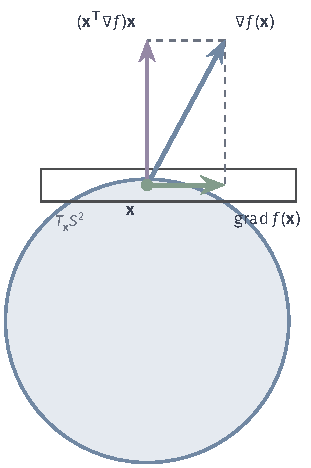
\includegraphics[width=52.7mm]{figures/05-optimization/06-constrained-optimization/tikz/mfo-tangent-projection/figure.pdf}
 \caption{起点$\bm{x}^{(0)}$处欧氏梯度的分解。蓝箭头是$\nabla f$，紫箭头是法向分量，绿箭头是切向分量即黎曼梯度，方框是切平面的一块。三个箭头按同一比例缩短到原长的$0.6$倍。}
 \label{fig:mfo-tangent-projection}
\end{BookInlineFigure}

\paragraph{一阶条件与Lagrange乘子}
现在把切向梯度与第~\ref{chap:constrained-optimality}章的乘子联系起来。由式~\eqref{eq:mfo-tangent}，$T_{\bm{x}}M$的正交投影可以写成
\[
 \bm{P}_{\bm{x}}=\bm{I}-\bm{J}^\top(\bm{J}\bm{J}^\top)^{-1}\bm{J},
\]
这里行满秩保证$\bm{J}\bm{J}^\top$可逆。

把投影代入式~\eqref{eq:mfo-projection-gradient}，并定义乘子
\begin{equation}
 \bm{\nu}(\bm{x})=-(\bm{J}\bm{J}^\top)^{-1}\bm{J}\nabla\bar{f}(\bm{x}),
 \label{eq:mfo-ls-multiplier}
\end{equation}
就得到
\begin{equation}
 \operatorname{grad}f(\bm{x})=\nabla\bar{f}(\bm{x})+\bm{J}(\bm{x})^\top\bm{\nu}(\bm{x})=\nabla_{\bm{x}}\mathcal{L}(\bm{x},\bm{\nu}(\bm{x})).
 \label{eq:mfo-grad-lagrange}
\end{equation}
所以黎曼梯度正是Lagrange函数对$\bm{x}$的梯度，乘子取使$\lVert\nabla\bar{f}+\bm{J}^\top\bm{\nu}\rVert_2$最小的最小二乘乘子。黎曼梯度为零，就是Lagrange乘子驻定条件。

球面上$h(\bm{x})=\bm{x}^\top\bm{x}-1$，$\bm{J}=2\bm{x}^\top$，$\bm{J}\bm{J}^\top=4$，代入式~\eqref{eq:mfo-ls-multiplier}得到
\[
 \nu(\bm{x})=-\frac14\cdot2\bm{x}^\top\bm{A}\bm{x}=-\frac12q(\bm{x}).
\]
梯度为零的条件$\bm{A}\bm{x}=q\bm{x}$说明，驻点恰好是$\bm{A}$的单位特征向量，并且$q$就是特征值。贯穿例有六个驻点$\pm\bm{e}_1,\pm\bm{e}_2,\pm\bm{e}_3$。

图~\ref{fig:mfo-rayleigh-landscape}是目标在球面上的等高线。红点$\bm{e}_1$周围的闭合曲线表明这里是极小点，$\bm{e}_3$是极大点，$\bm{e}_2$处等高线呈交叉状，它是鞍点。

\begin{BookInlineFigure}
 \centering
 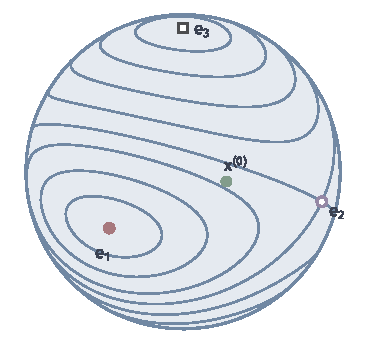
\includegraphics[width=62.0mm]{figures/05-optimization/06-constrained-optimization/matplotlib/mfo-rayleigh-landscape/figure.pdf}
 \caption{贯穿例的目标在单位球面上的等高线（蓝），只画朝向读者的半球。红点是极小点$\bm{e}_1$，紫圈是鞍点$\bm{e}_2$，方块是极大点$\bm{e}_3$，绿点是起点。背面半球的$-\bm{e}_1,-\bm{e}_2,-\bm{e}_3$有相同的情形。}
 \label{fig:mfo-rayleigh-landscape}
\end{BookInlineFigure}

\paragraph{切向曲率}
一阶条件分不开$\bm{e}_1,\bm{e}_2,\bm{e}_3$，需要二阶信息。\term{黎曼Hessian}（Riemannian Hessian）是切空间$T_{\bm{x}}M$到自身的对称线性算子，记为$\operatorname{Hess}f(\bm{x})$，定义为黎曼梯度沿切向量的协变导数，其几何来历可参考\BookChapterRef{chap:riemannian-geometry}{卷四第27章“黎曼几何”}。

诱导度量下的协变导数是先做普通方向导数再投影，所以只要把黎曼梯度光滑延拓成环境空间中的向量场$\bm{G}$，就有
\begin{equation}
 \operatorname{Hess}f(\bm{x})[\bm{v}]=\bm{P}_{\bm{x}}\,\mathrm{D}\bm{G}(\bm{x})[\bm{v}].
 \label{eq:mfo-hess-projection}
\end{equation}

球面上把式~\eqref{eq:mfo-rayleigh-grad}的右端在整个空间中当作$\bm{G}(\bm{x})$，方向导数是
\[
 \mathrm{D}\bm{G}(\bm{x})[\bm{v}]=\bm{A}\bm{v}-2(\bm{x}^\top\bm{A}\bm{v})\bm{x}-q(\bm{x})\bm{v}.
\]
第二项沿法向，投影后消失；第三项本身是切向的。于是
\begin{equation}
 \operatorname{Hess}f(\bm{x})[\bm{v}]=\bm{P}_{\bm{x}}\bigl(\bm{A}\bm{v}\bigr)-q(\bm{x})\bm{v},\qquad \bm{v}\perp\bm{x}.
 \label{eq:mfo-rayleigh-hess}
\end{equation}

这个式子里的$-q\bm{v}$值得留意。欧氏Hessian是$\bm{A}$，而切向曲率还要减去$q$，这一项来自约束本身的弯曲，由乘子项承担，下面马上看到。

在驻点上用这个公式。取$\bm{x}=\bm{e}_i$，$q=\lambda_i$，切空间由其余两个坐标向量张成，算子是对角的。三个驻点的切向曲率如表~\ref{tab:mfo-critical}所示。

\begin{BookInlineTable}
 \centering
 \caption{贯穿例的驻点，切向曲率由式~\eqref{eq:mfo-rayleigh-hess}算出。}
 \label{tab:mfo-critical}
 \begin{tabular}{llll}
  \toprule
  驻点 & $q$ & 切向曲率 & 类型\\
  \midrule
  $\pm\bm{e}_1$ & $1$ & $2-1=1,\ 4-1=3$ & 严格局部极小，全局极小\\
  $\pm\bm{e}_2$ & $2$ & $1-2=-1,\ 4-2=2$ & 鞍点\\
  $\pm\bm{e}_3$ & $4$ & $1-4=-3,\ 2-4=-2$ & 严格局部极大\\
  \bottomrule
 \end{tabular}
\end{BookInlineTable}

图~\ref{fig:mfo-critical-local}把三类驻点放到各自的切平面坐标里看。图中的函数值是把切向量先归一化回球面后计算的，局部形状与表中的符号一致。

\begin{BookInlineFigure}
 \centering
 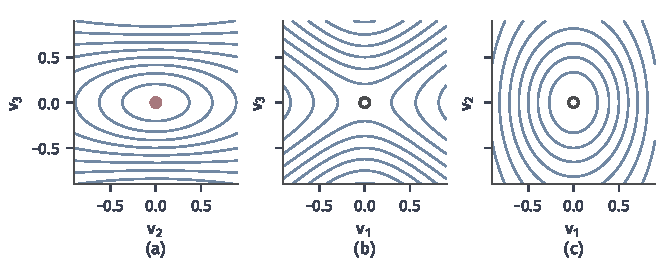
\includegraphics[width=112.0mm]{figures/05-optimization/06-constrained-optimization/matplotlib/mfo-critical-local/figure.pdf}
 \caption{三类驻点附近的局部形状。蓝线是$f(\bm{x}+\bm{v})/\lVert\bm{x}+\bm{v}\rVert_2^2$的等值线，这里的$f$在贯穿例中是二次齐次的，该式等于把$\bm{x}+\bm{v}$归一化后的目标值。$(v_i,v_j)$是切平面坐标。(a)~$\bm{e}_1$，碗形。(b)~$\bm{e}_2$，马鞍形。(c)~$\bm{e}_3$，倒扣的碗。}
 \label{fig:mfo-critical-local}
\end{BookInlineFigure}

\paragraph{曲率与Lagrange函数的Hessian}
为什么约束的弯曲会以乘子的形式进入？设$\bm{c}(t)$是$M$上的曲线，$\bm{c}(0)=\bm{x}$，$\bm{c}'(0)=\bm{v}$。由$h_j(\bm{c}(t))=0$求两次导，得到
\[
 \nabla h_j(\bm{x})^\top\bm{c}''(0)+\bm{v}^\top\nabla^2h_j(\bm{x})\bm{v}=0.
\]

现在求目标沿曲线的二阶导数，它是
\[
 (\bar{f}\circ\bm{c})''(0)=\bm{v}^\top\nabla^2\bar{f}\bm{v}+\nabla\bar{f}^\top\bm{c}''(0).
\]
由式~\eqref{eq:mfo-grad-lagrange}把$\nabla\bar{f}$换成黎曼梯度减去$\bm{J}^\top\bm{\nu}$，再利用上一式把$\nabla h_j^\top\bm{c}''(0)$换掉，就得到
\begin{equation}
 (\bar{f}\circ\bm{c})''(0)=\bm{v}^\top\nabla^2_{\bm{x}\bm{x}}\mathcal{L}(\bm{x},\bm{\nu}(\bm{x}))\bm{v}+\bigl\langle\operatorname{grad}f(\bm{x}),\bm{c}''(0)\bigr\rangle.
 \label{eq:mfo-second-along-curve}
\end{equation}

测地线的加速度是纯法向的，所以取$\bm{c}$为测地线时最后一项为零，左端就是$\langle\bm{v},\operatorname{Hess}f(\bm{x})[\bm{v}]\rangle$。这样切向曲率等于Lagrange函数的Hessian在切空间上的二次型：
\begin{equation}
 \langle\bm{v},\operatorname{Hess}f(\bm{x})[\bm{v}]\rangle=\bm{v}^\top\nabla^2_{\bm{x}\bm{x}}\mathcal{L}(\bm{x},\bm{\nu}(\bm{x}))\bm{v},\qquad\bm{v}\in T_{\bm{x}}M.
 \label{eq:mfo-hess-lagrange}
\end{equation}

球面上核对一下。Lagrange函数的Hessian是
\[
 \nabla^2_{\bm{x}\bm{x}}\mathcal{L}=\bm{A}+2\nu\bm{I}=\bm{A}-q\bm{I},
\]
所以二次型是$\bm{v}^\top\bm{A}\bm{v}-q\lVert\bm{v}\rVert_2^2$，与式~\eqref{eq:mfo-rayleigh-hess}相同。式~\eqref{eq:mfo-second-along-curve}最后那一项在第~\ref{sec:mfo-pullback}节还会用到。

\paragraph{二阶判别}
下面的定理把上述量组织成判别条件，要分清必要与充分。

\begin{theorem}[流形上的最优性条件]
 \label{thm:mfo-optimality}
 设$f$在黎曼流形$M$上二阶连续可微，$\bm{x}^\star\in M$。
 \begin{enumerate}
  \item 若$\bm{x}^\star$是局部极小点，则$\operatorname{grad}f(\bm{x}^\star)=\bm{0}$，且$\operatorname{Hess}f(\bm{x}^\star)$半正定。
  \item 若$\operatorname{grad}f(\bm{x}^\star)=\bm{0}$，且$\operatorname{Hess}f(\bm{x}^\star)$在$T_{\bm{x}^\star}M$上正定，则$\bm{x}^\star$是严格局部极小点。
 \end{enumerate}
\end{theorem}

\begin{proof}
 记指数映射为$\exp_{\bm{x}^\star}$，定义切空间上的函数
 \[
  \phi(\bm{v})=f(\exp_{\bm{x}^\star}(\bm{v})).
 \]

 指数映射在零点的微分是恒等映射，由反函数定理，它把零点的一个邻域微分同胚地映到$\bm{x}^\star$的一个邻域。

 因此$\bm{x}^\star$是$f$的（严格）局部极小点，当且仅当$\bm{0}$是$\phi$的（严格）局部极小点。对单位切向量$\bm{v}$，曲线$\gamma(t)=\exp_{\bm{x}^\star}(t\bm{v})$是测地线，于是
 \[
  \frac{\mathrm{d}}{\mathrm{d}t}\phi(t\bm{v})\Big|_{t=0}=\langle\operatorname{grad}f(\bm{x}^\star),\bm{v}\rangle,
  \qquad
  \frac{\mathrm{d}^2}{\mathrm{d}t^2}\phi(t\bm{v})\Big|_{t=0}=\langle\bm{v},\operatorname{Hess}f(\bm{x}^\star)[\bm{v}]\rangle.
 \]
 这说明$\phi$在零点的欧氏梯度和Hessian正是黎曼梯度和黎曼Hessian。把线性空间上无约束问题的一阶、二阶必要条件和二阶充分条件用到$\phi$上，就得到两个结论。
\end{proof}

两个条件之间有间隙，$\operatorname{Hess}f$半正定但不正定时，定理不作结论。取圆周上的$f(\bm{x})=x_2^3$，在点$(1,0)$处切向坐标为$\theta$，$f=\sin^3\theta$的一阶、二阶导数都为零，二阶必要条件成立，但$\theta<0$时函数值更小，这一点不是局部极小。

半正定也可能来自一整段极小点。取$\bm{A}=\operatorname{diag}(1,1,4)$，圆周$x_3=0$上每一点都是全局极小点，切向曲率有一个零方向，定理第二条不适用，这些点并不是孤立的。

定理也只是局部结论。圆周上的$\cos3\theta+0.3\cos\theta$在$\theta=\pi$附近和$\theta=\pm\pi/3$附近都有严格局部极小，函数值分别约为$-1.30$和$-0.85$，后者满足二阶充分条件却不是全局极小。

Rayleigh商是一个少见的例外，局部极小都是全局极小。设$\bm{x}$是特征向量，特征值$\lambda>\lambda_1$，取$\lambda_1$的单位特征向量$\bm{v}$，它与$\bm{x}$正交，由式~\eqref{eq:mfo-rayleigh-hess}得到
\[
 \langle\bm{v},\operatorname{Hess}f(\bm{x})[\bm{v}]\rangle=\lambda_1-\lambda<0.
\]
所以满足二阶必要条件的驻点只能属于最小特征值。这个结论来自目标的特殊结构，不能推广到一般流形问题。

\section{迭代的几何运算}
\label{sec:mfo-operations}

现在假定当前点$\bm{x}$处已经算出一个切向候选步$\bm{v}\in T_{\bm{x}}M$。欧氏空间里接下来的事情都是加减法，到了流形上有三件事要重新回答：走完之后怎样回到集合上，怎样评价这一步好不好，历史上的向量在新点怎样使用。

图~\ref{fig:mfo-iteration-loop}是后面所有算法共用的循环。切向候选步由各节的方法给出，其余三个方框分别由下面三小节回答。这里只讨论能在计算机上执行的运算，切空间、联络和指数映射的定义仍以卷四为准。

\begin{BookInlineFigure}
 \centering
 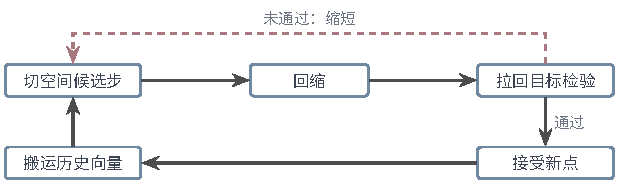
\includegraphics[width=104.7mm]{figures/05-optimization/06-constrained-optimization/tikz/mfo-iteration-loop/figure.pdf}
 \caption{流形优化的一轮迭代。切空间里产生候选步，回缩把它变成流形上的候选点，再用拉回后的目标判断是否接受；接受后把需要保留的历史向量搬到新点的切空间。红色虚线表示判断未通过时缩短步长或半径。}
 \label{fig:mfo-iteration-loop}
\end{BookInlineFigure}

\subsection{回缩}
\label{sec:mfo-retraction}

\paragraph{用球面看需要什么}
从$\bm{x}$走到$\bm{x}+\bm{v}$后，最自然的修正是除以长度，把点拉回球面：
\begin{equation}
 R_{\bm{x}}(\bm{v})=\frac{\bm{x}+\bm{v}}{\lVert\bm{x}+\bm{v}\rVert_2}=\frac{\bm{x}+\bm{v}}{\sqrt{1+\lVert\bm{v}\rVert_2^2}}.
 \label{eq:mfo-sphere-retraction}
\end{equation}
第二个等号用到$\bm{x}\perp\bm{v}$和勾股定理。这个映射有两条关键性质：零步不动，并且走很小的一步时，它和切向量给出的方向一致。

把第二条写成曲线的语言。令$\bm{c}(t)=R_{\bm{x}}(t\bm{v})$，把分母按$t$展开，得到
\[
 \bm{c}(t)=(\bm{x}+t\bm{v})\Bigl(1-\frac12t^2\lVert\bm{v}\rVert_2^2+O(t^4)\Bigr).
\]
由此读出$\bm{c}(0)=\bm{x}$，$\bm{c}'(0)=\bm{v}$，加速度$\bm{c}''(0)=-\lVert\bm{v}\rVert_2^2\bm{x}$沿法向。

这两条性质正是我们真正需要的，再多的要求（例如走出的曲线恰好是测地线）对一阶信息没有帮助。于是有下面的定义。

\begin{definition}[回缩]
 \label{def:mfo-retraction}
 流形$M$上的\term{回缩}（retraction）是一族光滑映射$R_{\bm{x}}:U_{\bm{x}}\to M$，其中$U_{\bm{x}}$是$T_{\bm{x}}M$中包含零的开集，并且对所有$\bm{x}\in M$，$\bm{v}\in T_{\bm{x}}M$有
 \begin{equation}
  R_{\bm{x}}(\bm{0})=\bm{x},\qquad
  \frac{\mathrm{d}}{\mathrm{d}t}R_{\bm{x}}(t\bm{v})\Big|_{t=0}=\bm{v}.
  \label{eq:mfo-retraction-def}
 \end{equation}
 若进一步对所有$\bm{v}$，曲线$\bm{c}(t)=R_{\bm{x}}(t\bm{v})$的加速度满足$\bm{P}_{\bm{x}}\bm{c}''(0)=\bm{0}$，则称它为\term{二阶回缩}（second-order retraction）。
\end{definition}

二阶条件的提法依赖诱导度量：对嵌入子流形，它说的是加速度的切向分量为零。指数映射是最典型的二阶回缩，因为测地线加速度的切向分量恒为零。式~\eqref{eq:mfo-sphere-retraction}由上面的展开也是二阶回缩。

\paragraph{回缩不等于指数映射}
图~\ref{fig:mfo-retraction-cut}(a)在穿过球心的截面上比较两种走法。切向量长度为$s$时，指数映射沿大圆走过角度$s$，归一化走过角度$\arctan s$。

\begin{BookInlineFigure}
 \centering
 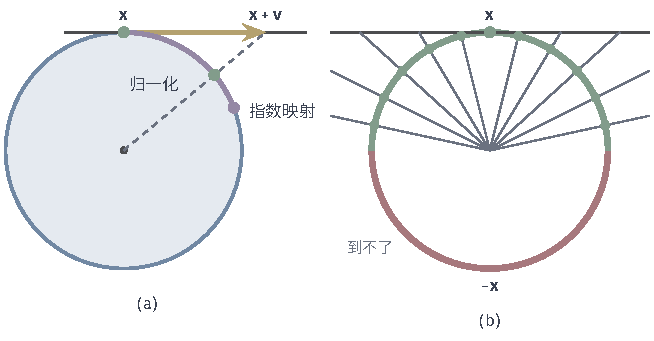
\includegraphics[width=110.8mm]{figures/05-optimization/06-constrained-optimization/tikz/mfo-retraction-cut/figure.pdf}
 \caption{球面的截面。(a)~黄箭头是长度$1.2$的切向量，归一化把它的端点沿虚线径向拉回到绿点，紫弧是指数映射走过的路，端点在紫点。(b)~切线上的点全都被归一化映到上半圆（绿）。下半圆（红）到不了，对跖点$-\bm{x}$也到不了。}
 \label{fig:mfo-retraction-cut}
\end{BookInlineFigure}

两者的差在小步时很小。由$\arctan s=s-s^3/3+O(s^5)$，角度差是$s^3/3$的量级，这是图~\ref{fig:mfo-retraction-error}(b)的斜率$3$。步子大了差距才明显：$s\to\infty$时归一化只能逼近$\pi/2$，而指数映射走过的角度不断增长。

\begin{BookInlineFigure}
 \centering
 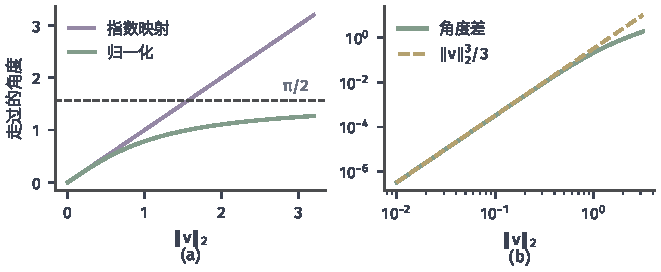
\includegraphics[width=112.0mm]{figures/05-optimization/06-constrained-optimization/matplotlib/mfo-retraction-error/figure.pdf}
 \caption{球面上切向量长度$\lVert\bm{v}\rVert_2$与走过的角度。(a)~指数映射（紫）的角度等于长度，归一化（绿）的角度不超过$\pi/2$。(b)~双对数坐标下两者的角度差（绿）与$\lVert\bm{v}\rVert_2^3/3$（黄虚线）在小步时重合。}
 \label{fig:mfo-retraction-error}
\end{BookInlineFigure}

把切平面整张折到球面上，就看到回缩的全貌。图~\ref{fig:mfo-retraction-grid}中，切平面上等间距的同心圆经过归一化后向边缘挤压，径向的射线变成大圆。这也提醒我们，回缩不是等距的，切空间里的长度只在原点附近才代表流形上走过的距离。

\begin{BookInlineFigure}
 \centering
 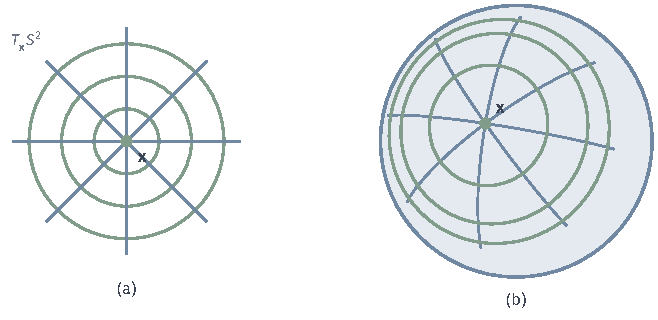
\includegraphics[width=111.3mm]{figures/05-optimization/06-constrained-optimization/tikz/mfo-retraction-grid/figure.pdf}
 \caption{归一化回缩把切平面折到球面上。(a)~切平面上半径$0.5,1,1.5$的同心圆（绿）与八条射线（蓝）。(b)~它们在回缩下的像，同心圆的间距向外收紧，射线变成大圆的一段。}
 \label{fig:mfo-retraction-grid}
\end{BookInlineFigure}

\paragraph{定义域}
归一化公式对所有切向量都有定义，因为$\bm{x}\perp\bm{v}$保证$\bm{x}+\bm{v}\neq\bm{0}$，但它的像只覆盖开上半球，如图~\ref{fig:mfo-retraction-cut}(b)所示。定义~\ref{def:mfo-retraction}只要求在零的邻域内有定义，这对迭代是足够的，因为每步只需要局部信息。

一般回缩可能只在局部有定义，分解还可能有多种选择。选择不固定就会使映射不光滑，下面的矩阵例子就有这个问题。

\paragraph{Stiefel流形上的回缩}
取$\bm{X}\in\mathrm{St}(k,n)$，切向量$\bm{\Delta}$满足$\bm{X}^\top\bm{\Delta}$反对称。把$\bm{X}+\bm{\Delta}$作QR分解$\bm{X}+\bm{\Delta}=\bm{Q}\bm{R}$，其中$\bm{R}$上三角且对角元为正，取$\bm{Q}$作为新点：
\begin{equation}
 R_{\bm{X}}^{\mathrm{QR}}(\bm{\Delta})=\bm{Q}.
 \label{eq:mfo-qr-retraction}
\end{equation}

固定对角元为正这个选择是必要的，否则列的符号可以任意翻转，映射甚至不连续。分解一定存在且唯一，因为$\bm{X}^\top\bm{\Delta}$反对称使两个交叉项抵消：
\[
 (\bm{X}+\bm{\Delta})^\top(\bm{X}+\bm{\Delta})=\bm{I}+\bm{\Delta}^\top\bm{\Delta}\succ\bm{0},
\]
所以$\bm{X}+\bm{\Delta}$列满秩。

下面核对一阶一致性。令$\bm{X}+t\bm{\Delta}=\bm{Q}(t)\bm{R}(t)$，$\bm{Q}(0)=\bm{X}$，$\bm{R}(0)=\bm{I}$。对$t$求导并在$t=0$左乘$\bm{X}^\top$，得到
\[
 \bm{X}^\top\bm{\Delta}=\bm{X}^\top\bm{Q}'(0)+\bm{R}'(0).
\]

左端反对称，右端第一项也反对称（对$\bm{Q}(t)^\top\bm{Q}(t)=\bm{I}$求导得到），所以$\bm{R}'(0)$既反对称又上三角，只能是零。代回求导式就得到$\bm{Q}'(0)=\bm{\Delta}$。

第二种构造用极分解，把$\bm{X}+\bm{\Delta}$的列正交化的同时尽量少动它：
\begin{equation}
 R_{\bm{X}}^{\mathrm{pol}}(\bm{\Delta})=(\bm{X}+\bm{\Delta})\bigl(\bm{I}+\bm{\Delta}^\top\bm{\Delta}\bigr)^{-1/2}.
 \label{eq:mfo-polar-retraction}
\end{equation}

结果确实在流形上：列满秩矩阵右乘$(\bm{Y}^\top\bm{Y})^{-1/2}$后列标准正交。把逆平方根展开，得到
\[
 \bm{C}(t)=(\bm{X}+t\bm{\Delta})\Bigl(\bm{I}-\frac12t^2\bm{\Delta}^\top\bm{\Delta}+O(t^4)\Bigr).
\]
于是$\bm{C}'(0)=\bm{\Delta}$，$\bm{C}''(0)=-\bm{X}\bm{\Delta}^\top\bm{\Delta}$。

后者形如$\bm{X}\bm{B}$，其中$\bm{B}$对称。为了判断它的切向分量，写出$\mathrm{St}(k,n)$的切向投影
\begin{equation}
 \bm{P}_{\bm{X}}(\bm{Z})=\bm{Z}-\bm{X}\operatorname{sym}(\bm{X}^\top\bm{Z}),\qquad \operatorname{sym}(\bm{B})=\frac12(\bm{B}+\bm{B}^\top).
 \label{eq:mfo-stiefel-projection}
\end{equation}
把$\bm{Z}=\bm{X}\bm{B}$代入，得到$\bm{X}\bm{B}-\bm{X}\bm{B}=\bm{0}$，所以极分解回缩是二阶回缩。QR回缩一般只是一阶的，下面的例子中它的加速度有非零的切向分量。

用具体数字比较两种构造。在$\mathrm{St}(2,3)$上取
\[
 \bm{X}=\begin{bmatrix}1&0\\0&1\\0&0\end{bmatrix},\qquad
 \bm{\Delta}=\begin{bmatrix}0&0\\0&0\\1&1\end{bmatrix},\qquad
 \bm{Y}=\bm{X}+\bm{\Delta}=\begin{bmatrix}1&0\\0&1\\1&1\end{bmatrix}.
\]
这里$\bm{X}^\top\bm{\Delta}=\bm{0}$，是切向量。

QR分解按列正交化。第一列除以$\sqrt2$，第二列减去在第一列上的投影再除以长度，于是
\[
 \bm{q}_1=\frac{1}{\sqrt2}(1,0,1)^\top,\qquad
 \bm{q}_2=\frac{1}{\sqrt6}(-1,2,1)^\top.
\]

极分解要用$\bm{I}+\bm{\Delta}^\top\bm{\Delta}$的逆平方根。这个矩阵是
\[
 \bm{I}+\bm{\Delta}^\top\bm{\Delta}=\begin{bmatrix}2&1\\1&2\end{bmatrix},
\]
特征值为$3,1$，特征向量为$(1,1)^\top/\sqrt2$和$(1,-1)^\top/\sqrt2$，算出来的结果是
\[
 R_{\bm{X}}^{\mathrm{pol}}(\bm{\Delta})\approx\begin{bmatrix}0.7887&-0.2113\\-0.2113&0.7887\\0.5774&0.5774\end{bmatrix}.
\]

沿曲线$R_{\bm{X}}(t\bm{\Delta})$算加速度的切向分量，极分解得到零，QR回缩得到
\[
 \bm{P}_{\bm{X}}\bm{C}''(0)=\begin{bmatrix}0&-1\\1&0\\0&0\end{bmatrix},
\]
不是零，这印证了两者阶数的差别。

图~\ref{fig:mfo-stiefel-qr-polar}画出两个结果。QR分解保留第一列的方向，把调整都压给后面的列，极分解则两列对称地调整。两个新点张成同一个平面，这个事实在第~\ref{sec:mfo-representation}节会派上用场。

\begin{BookInlineFigure}
 \centering
 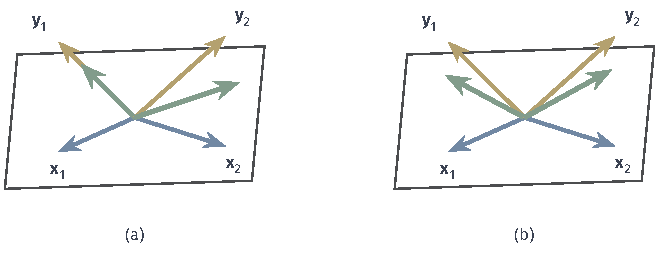
\includegraphics[width=111.6mm]{figures/05-optimization/06-constrained-optimization/tikz/mfo-stiefel-qr-polar/figure.pdf}
 \caption{$\mathrm{St}(2,3)$上的两种回缩。蓝箭头是当前两列，黄箭头是$\bm{X}+\bm{\Delta}$的两列，绿箭头是回缩结果，方框是$\bm{y}_1,\bm{y}_2$张成的平面。(a)~QR分解：第一列方向不变。(b)~极分解：两列对称调整。}
 \label{fig:mfo-stiefel-qr-polar}
\end{BookInlineFigure}

\paragraph{回缩、指数映射与最近点}
第三个候选是把$\bm{x}+\bm{v}$投影到$M$上的最近点。球面上它恰好就是归一化；$\mathrm{St}(k,n)$上在Frobenius范数下恰好就是极分解，例中极分解结果到$\bm{Y}$的距离约为$0.732$，QR结果约为$0.850$。

但回缩并不要求求解最近点问题。QR回缩不是最近点，同样满足定义，而且通常更便宜。在一般曲面上，最近点可能需要迭代才能算出，甚至不唯一。表~\ref{tab:mfo-retraction-compare}比较三者。

\begin{BookInlineTable}
 \centering
 \caption{三种回到流形的方式。“二阶”的结论对最近点投影要求流形足够光滑，表中代价按一次运算计。}
 \label{tab:mfo-retraction-compare}
 \begin{tabular}{llll}
  \toprule
  方式 & 阶 & 球面 & Stiefel\\
  \midrule
  指数映射 & 二阶 & $O(n)$ & 需矩阵指数\\
  最近点投影 & 二阶 & $O(n)$ & 需SVD\\
  QR回缩 & 一阶 & 同归一化 & 约$O(nk^2)$\\
  \bottomrule
 \end{tabular}
\end{BookInlineTable}

\subsection{目标拉回}
\label{sec:mfo-pullback}

\paragraph{把问题搬到同一个切空间}
候选步是切空间中的向量，而目标定义在流形上。把两者复合，就得到切空间上的普通函数，这是后面评价候选步的唯一依据。

\begin{definition}[拉回目标]
 \label{def:mfo-pullback}
 在$\bm{x}\in M$处，目标$f$的\term{拉回}（pullback）是切空间上的函数
 \begin{equation}
  \hat{f}_{\bm{x}}(\bm{v})=f\bigl(R_{\bm{x}}(\bm{v})\bigr),\qquad\bm{v}\in U_{\bm{x}}.
  \label{eq:mfo-pullback}
 \end{equation}
\end{definition}

这个定义的好处是，$\hat{f}_{\bm{x}}$活在线性空间上，前面各章的工具（Taylor展开、Armijo条件、预测下降）都可以直接使用。

贯穿例在$\bm{x}^{(0)}$的切平面上取一组标准正交基：
\[
 \bm{E}_1=\frac13(1,-2,2)^\top,\qquad
 \bm{E}_2=\frac13(2,-1,-2)^\top.
\]
可以检查$\bm{x}^{(0)},\bm{E}_1,\bm{E}_2$两两正交且长度为一。

沿$\bm{v}=s\bm{E}_2$拉回。需要的内积是$\bm{x}^{(0)\top}\bm{A}\bm{E}_2=-\tfrac89$和$\bm{E}_2^\top\bm{A}\bm{E}_2=\tfrac{22}{9}$，代入归一化回缩，得到
\begin{equation}
 \hat{f}_{\bm{x}^{(0)}}(s\bm{E}_2)=\frac{1}{1+s^2}\cdot\frac12\Bigl(\frac{16}{9}-\frac{16}{9}s+\frac{22}{9}s^2\Bigr)=\frac{8-8s+11s^2}{9(1+s^2)}.
 \label{eq:mfo-pullback-line}
\end{equation}

\paragraph{一阶与二阶变化}
下面的引理说明，拉回在零点的一阶信息总是黎曼梯度，二阶信息则取决于回缩的加速度。

\begin{lemma}[拉回的导数]
 \label{lem:mfo-pullback-derivatives}
 设$M$是嵌入子流形，取诱导度量，$R$是回缩，$\bm{v}\in T_{\bm{x}}M$，$\bm{c}(t)=R_{\bm{x}}(t\bm{v})$。则
 \begin{equation}
  \nabla\hat{f}_{\bm{x}}(\bm{0})=\operatorname{grad}f(\bm{x}),
  \label{eq:mfo-pullback-grad}
 \end{equation}
 \begin{equation}
  \langle\bm{v},\nabla^2\hat{f}_{\bm{x}}(\bm{0})\bm{v}\rangle=\langle\bm{v},\operatorname{Hess}f(\bm{x})[\bm{v}]\rangle+\bigl\langle\operatorname{grad}f(\bm{x}),\bm{c}''(0)\bigr\rangle.
  \label{eq:mfo-pullback-hess}
 \end{equation}
\end{lemma}

\begin{proof}
 由复合函数求导和式~\eqref{eq:mfo-retraction-def}，
 \[
  \frac{\mathrm{d}}{\mathrm{d}t}\hat{f}_{\bm{x}}(t\bm{v})\Big|_{t=0}=\mathrm{d}f_{\bm{x}}[\bm{c}'(0)]=\mathrm{d}f_{\bm{x}}[\bm{v}]=\langle\operatorname{grad}f(\bm{x}),\bm{v}\rangle,
 \]
 这是式~\eqref{eq:mfo-pullback-grad}。

 $\hat{f}_{\bm{x}}(t\bm{v})=f(\bm{c}(t))$，把式~\eqref{eq:mfo-second-along-curve}用到曲线$\bm{c}$上，再用式~\eqref{eq:mfo-hess-lagrange}替换第一项，就得到式~\eqref{eq:mfo-pullback-hess}。
\end{proof}

式~\eqref{eq:mfo-pullback-hess}的附加项给出了两条实用的结论。第一，二阶回缩的$\bm{c}''(0)$是法向的，黎曼梯度是切向的，附加项为零，拉回Hessian等于黎曼Hessian。第二，在驻点上$\operatorname{grad}f=\bm{0}$，对任何回缩附加项都为零，所以一般回缩在驻点处两者也相等。

一般回缩在非驻点处可能有差别。圆周的例子最容易看清。取角度$\theta$为坐标，目标
\[
 \varphi(\theta)=\frac12\bigl(\cos^2\theta+4\sin^2\theta\bigr),\qquad
 \varphi'(\theta)=\frac32\sin2\theta,\qquad
 \varphi''(\theta)=3\cos2\theta.
\]

比较三种回缩：指数映射$\theta+s$，归一化$\theta+\arctan s$，以及一个人为构造的一阶回缩$\theta+s+\tfrac12s^2$。第三个满足定义，但沿圆周的加速度是$1$，不是二阶的。对它求拉回的二阶导数，得到
\[
 \hat{f}''(0)=\varphi''(\theta)+\varphi'(\theta).
\]

在$\theta=\pi/6$处，$\varphi'=3\sqrt3/4\approx1.299$，$\varphi''=1.5$。前两种回缩的拉回二阶导数都是$1.5$，第三种是$2.799$。在驻点$\theta=0$处$\varphi'=0$，三者都是$3$。图~\ref{fig:mfo-pullback-curvature}画出这个差别。

\begin{BookInlineFigure}
 \centering
 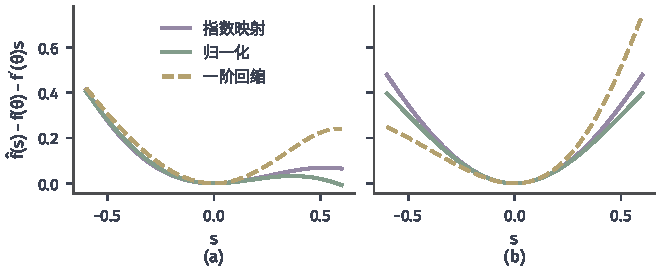
\includegraphics[width=112.0mm]{figures/05-optimization/06-constrained-optimization/matplotlib/mfo-pullback-curvature/figure.pdf}
 \caption{圆周上目标扣除一阶项后的拉回$\hat{f}(s)-\varphi(\theta)-\varphi'(\theta)s$。紫线、绿线、黄虚线分别对应指数映射、归一化与一阶回缩$\theta+s+s^2/2$。(a)~非驻点$\theta=\pi/6$，黄虚线在零点的曲率明显更大。(b)~驻点$\theta=0$，三条曲线在零点处曲率相同。}
 \label{fig:mfo-pullback-curvature}
\end{BookInlineFigure}

\paragraph{用拉回评价候选步}
式~\eqref{eq:mfo-pullback-grad}和式~\eqref{eq:mfo-pullback-hess}支持下面这个切空间二次模型：
\begin{equation}
 m_{\bm{x}}(\bm{v})=f(\bm{x})+\langle\operatorname{grad}f(\bm{x}),\bm{v}\rangle+\frac12\langle\bm{v},\operatorname{Hess}f(\bm{x})[\bm{v}]\rangle.
 \label{eq:mfo-model}
\end{equation}

在贯穿例的方向上核对。沿$s\bm{E}_2$，切向曲率是
\[
 \langle\bm{E}_2,(\bm{A}-q\bm{I})\bm{E}_2\rangle=\frac{22}{9}-\frac{16}{9}=\frac23,
\]
模型是
\[
 m(s\bm{E}_2)=\frac89-\frac89s+\frac13s^2.
\]

用式~\eqref{eq:mfo-pullback-line}减去模型，分子通分后得到
\[
 \hat{f}_{\bm{x}^{(0)}}(s\bm{E}_2)-m(s\bm{E}_2)=\frac{8s^3-3s^4}{9(1+s^2)}.
\]
误差是$s^3$量级，这正是二阶回缩的效果。$s=0.1$时误差约为$8.5\times10^{-4}$，$s=1$时误差是$\tfrac{5}{18}$，模型已不可信，这是信赖域要处理的问题。

\subsection{向量搬运}
\label{sec:mfo-transport}

\paragraph{为什么需要搬运}
共轭梯度要把上一轮的方向和当前梯度相加，拟Newton要算两点梯度之差。欧氏空间里这些都是普通的加减法，流形上却有一个类型错误：旧向量在$T_{\bm{x}}M$中，新向量在$T_{\bm{y}}M$中，两者属于不同的线性空间。

在球面上，不同点的切平面是不同的平面，直接相加得到的向量一般不再切于任何一点。例如$\bm{x}^{(0)}$和$\bm{x}^{(1)}$处的两个切向量之和，通常与$\bm{x}^{(1)}$有非零内积。需要先把旧向量搬到新切空间。

\begin{definition}[向量搬运]
 \label{def:mfo-vector-transport}
 伴随回缩$R$的\term{向量搬运}（vector transport）是一族映射，对$\bm{x}\in M$和$\bm{\eta}\in T_{\bm{x}}M$给出线性映射$\mathcal{T}_{\bm{\eta}}$，它把$T_{\bm{x}}M$映到点$R_{\bm{x}}(\bm{\eta})$的切空间，且随$(\bm{x},\bm{\eta})$光滑变化，并满足$\mathcal{T}_{\bm{0}}=\mathrm{id}$。
\end{definition}

定义只要求三件事：结果落在新切空间中（一致性），对被搬运的向量是线性的，零步时什么也不做。它不要求保持长度和内积。后面需要这些额外性质时，要逐个核对。为了书写简洁，起点$\bm{x}$、终点$\bm{y}=R_{\bm{x}}(\bm{\eta})$明确时，记成$\mathcal{T}_{\bm{x}\to\bm{y}}$。

\paragraph{三种具体搬运}
第一种是\term{投影搬运}（projection transport），把旧向量看作环境空间的向量，投影到新切空间：
\begin{equation}
 \mathcal{T}^{\mathrm{P}}_{\bm{x}\to\bm{y}}(\bm{v})=\bm{P}_{\bm{y}}\bm{v}.
 \label{eq:mfo-projection-transport}
\end{equation}
它只对嵌入子流形可用，计算便宜。正交投影不会增加长度，但一般会减小长度。

第二种是\term{平行移动}（parallel transport），即卷四定义的沿曲线协变导数为零的搬运，它是等距的。球面上沿大圆从$\bm{x}$到$\bm{y}$有闭式：
\begin{equation}
 \mathcal{T}^{\parallel}_{\bm{x}\to\bm{y}}(\bm{v})=\bm{v}-\frac{\langle\bm{x}+\bm{y},\bm{v}\rangle}{1+\langle\bm{x},\bm{y}\rangle}(\bm{x}+\bm{y}).
 \label{eq:mfo-parallel-transport}
\end{equation}
这里要求$\bm{y}\neq-\bm{x}$。

下面验证结果确实切于$\bm{y}$且长度不变。记
\[
 c=\langle\bm{x},\bm{y}\rangle,\qquad a=\langle\bm{x}+\bm{y},\bm{v}\rangle.
\]

由$\bm{v}\perp\bm{x}$有$\langle\bm{y},\bm{v}\rangle=a$，又$\langle\bm{x}+\bm{y},\bm{y}\rangle=1+c$，于是
\[
 \langle\bm{y},\mathcal{T}^{\parallel}\bm{v}\rangle=a-\frac{a}{1+c}(1+c)=0.
\]

再用$\lVert\bm{x}+\bm{y}\rVert_2^2=2+2c$算长度：
\[
 \lVert\mathcal{T}^{\parallel}\bm{v}\rVert_2^2=\lVert\bm{v}\rVert_2^2-\frac{2a^2}{1+c}+\frac{a^2(2+2c)}{(1+c)^2}=\lVert\bm{v}\rVert_2^2.
\]

第三种是\term{微分回缩}（differentiated retraction），直接用回缩曲线的速度：
\[
 \mathcal{T}^{\mathrm{D}}_{\bm{\eta}}(\bm{v})=\frac{\mathrm{d}}{\mathrm{d}t}R_{\bm{x}}(\bm{\eta}+t\bm{v})\Big|_{t=0}.
\]
它的好处是下一节的线搜索导数恰好用这个向量。球面归一化沿搜索方向$\bm{d}$，设$\bm{y}=R_{\bm{x}}(\alpha\bm{d})$，$r=\lVert\bm{x}+\alpha\bm{d}\rVert_2$，求导得到
\[
 \frac{\mathrm{d}}{\mathrm{d}\tau}R_{\bm{x}}\bigl((\alpha+\tau)\bm{d}\bigr)\Big|_{\tau=0}=\frac{1}{r}\bm{P}_{\bm{y}}\bm{d}.
\]
所以此时投影搬运与微分回缩只差一个正的倍数$r$。

\paragraph{搬运结果的比较}
图~\ref{fig:mfo-transport}对比了切向量在两点之间的搬运。把$\bm{v}$平移到$\bm{y}$得到的副本并不切于球面（灰色虚线）。投影把副本垂直压到切平面上，长度变短；平行移动沿大圆旋转切平面，长度不变。

\begin{BookInlineFigure}
 \centering
 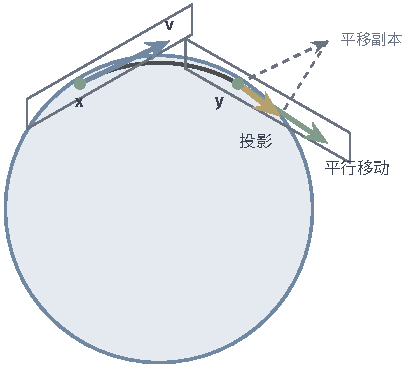
\includegraphics[width=70.0mm]{figures/05-optimization/06-constrained-optimization/tikz/mfo-transport/figure.pdf}
 \caption{把切向量$\bm{v}$（蓝）从$\bm{x}$搬到$\bm{y}$。深灰弧是连接两点的大圆，两个方框是切平面。灰色虚线箭头是平移的副本，不切于球面。黄箭头是投影结果，长度缩短；绿箭头是平行移动结果，长度与$\bm{v}$相同。}
 \label{fig:mfo-transport}
\end{BookInlineFigure}

用贯穿例算一次。第~\ref{sec:mfo-rgd}节将得到$\bm{x}^{(1)}\approx(0.8418,0.5388,-0.0337)^\top$，它与起点的内积约为$0.9091$。把基向量$\bm{E}_1,\bm{E}_2$搬到$\bm{x}^{(1)}$，投影的结果范数约为$0.9949$和$0.9147$，内积约为$0.0408$，平行移动的结果仍是标准正交的。

投影缩短的量取决于向量与连线方向的夹角。沿大圆方向的向量缩短最多，缩短比例等于两点内积。负梯度方向恰好是大圆方向，$\lVert\bm{g}^{(0)}\rVert_2\approx0.9162$的向量投影后长度约为$0.8330$，比值$0.9091$。

因此投影搬运不是等距的：它让向量落进了新切空间，但没有保持内积。若$\bm{y}\perp\bm{x}$，投影还会把沿连线方向的向量压成零，这时映射不可逆。表~\ref{tab:mfo-transport-compare}列出后面的算法需要核对的性质。

\begin{BookInlineTable}
 \centering
 \caption{三种搬运的性质，以球面归一化回缩为例。可逆一栏的$c=\langle\bm{x},\bm{y}\rangle$；一般流形上的平行移动要解常微分方程。}
 \label{tab:mfo-transport-compare}
 \begin{tabular}{llll}
  \toprule
  搬运 & 长度 & 可逆 & 代价\\
  \midrule
  投影 & 一般缩短 & 需$c\neq0$ & $O(n)$\\
  平行移动 & 保持 & 是 & $O(n)$\\
  微分回缩 & 沿步方向缩到$1/r^2$倍 & 需$c\neq0$ & $O(n)$\\
  \bottomrule
 \end{tabular}
\end{BookInlineTable}

\section{一阶方法}
\label{sec:mfo-first-order}

三种几何运算齐备后，先看只用一阶信息的方法。于是要问：负切向梯度加回缩为什么能下降，步长如何选择，以及搬运历史方向怎样加快收敛又带来了哪些新的检查项？

\subsection{黎曼梯度下降}
\label{sec:mfo-rgd}

\paragraph{主要思想}
\term{黎曼梯度下降}（Riemannian gradient descent）在当前切空间中沿负梯度取步，再用回缩回到流形：
\begin{equation}
 \bm{x}^{(t+1)}=R_{\bm{x}^{(t)}}\bigl(-\alpha^{(t)}\bm{g}^{(t)}\bigr),\qquad\bm{g}^{(t)}=\operatorname{grad}f(\bm{x}^{(t)}).
 \label{eq:mfo-rgd}
\end{equation}

为什么这一步能下降？记$\phi(\alpha)=\hat{f}_{\bm{x}}(-\alpha\bm{g})$，这是一个普通的一元函数。由式~\eqref{eq:mfo-pullback-grad}，
\[
 \phi'(0)=\langle\operatorname{grad}f(\bm{x}),-\bm{g}\rangle=-\lVert\bm{g}\rVert_2^2<0.
\]
所以只要$\bm{g}\neq\bm{0}$，足够小的步长一定使目标下降。这个结论只用了回缩的一阶一致性，不需要二阶回缩。

步长的选择与欧氏情形完全平行，只是把比较对象换成拉回函数。Armijo条件要求
\begin{equation}
 f\bigl(R_{\bm{x}}(-\alpha\bm{g})\bigr)\leq f(\bm{x})-c_1\alpha\lVert\bm{g}\rVert_2^2.
 \label{eq:mfo-armijo}
\end{equation}
下降的检验必须针对回缩后的点，切平面上的点$\bm{x}-\alpha\bm{g}$根本不可行，其函数值没有意义。

\needspace{6\baselineskip}
\paragraph{变量}
\begin{itemize}
 \item $\bm{x}^{(t)}\in\mathbb{R}^3$：球面上的当前点，长度为一。
 \item $q^{(t)}$：Rayleigh商的取值，标量。
 \item $\bm{g}^{(t)}$：黎曼梯度，与$\bm{x}^{(t)}$垂直的三维向量。
 \item $\alpha$：当前试探步长；$c_1=\tfrac14$是Armijo常数，缩减因子取$\tfrac12$。
\end{itemize}

\paragraph{初始化}
取$\bm{x}^{(0)}$，初始试探步长$\alpha_0=1$，停止容差$\lVert\bm{g}^{(t)}\rVert_2\leq10^{-6}$。例中$\bm{x}^{(0)}=\tfrac13(2,2,1)^\top$，$f(\bm{x}^{(0)})=\tfrac89$。

\needspace{6\baselineskip}
\paragraph{每轮更新}
\begin{enumerate}
 \item 由式~\eqref{eq:mfo-rayleigh-grad}算$\bm{g}^{(t)}$。例中第$0$轮已算得
 \[
  \bm{g}^{(0)}=\frac{1}{27}(-14,4,20)^\top,\qquad\lVert\bm{g}^{(0)}\rVert_2^2=\frac{68}{81}.
 \]

 \item 令$\alpha=\alpha_0$，按式~\eqref{eq:mfo-sphere-retraction}算试探点，并检验式~\eqref{eq:mfo-armijo}，不满足时$\alpha$减半。例中第$0$轮先试$\alpha=1$：
 \[
  \bm{x}^{(0)}-\bm{g}^{(0)}=\frac{1}{27}(32,14,-11)^\top.
 \]
 归一化后的点是$(0.8738,0.3823,-0.3004)^\top$，目标值$0.7084$，下降$0.1805$，低于要求的$\tfrac14\cdot\tfrac{68}{81}\approx0.2099$，拒绝。

 \item 例中减半后试$\alpha=\tfrac12$，得到
 \[
  \bm{x}^{(0)}-\tfrac12\bm{g}^{(0)}=\frac{1}{27}(25,16,-1)^\top.
 \]
 由勾股定理，长度的平方是$1+\tfrac14\cdot\tfrac{68}{81}=\tfrac{98}{81}$，长度是$\tfrac{7\sqrt2}{9}$。

 \item 接受时令$\bm{x}^{(t+1)}$为该试探点。例中
 \[
  \bm{x}^{(1)}=\frac{(25,16,-1)^\top}{21\sqrt2}\approx(0.8418,0.5388,-0.0337)^\top.
 \]
 目标值$0.6468$，下降$0.2421$，超过要求的$0.1049$，接受。
\end{enumerate}

图~\ref{fig:mfo-rgd-step}画出这一轮的几何：两个候选点都在切平面上，沿径向回到球面后才可以比较。

\begin{BookInlineFigure}
 \centering
 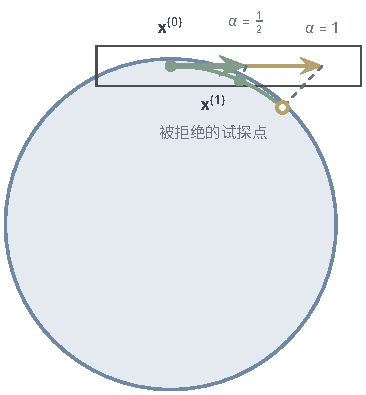
\includegraphics[width=62.0mm]{figures/05-optimization/06-constrained-optimization/tikz/mfo-rgd-step/figure.pdf}
 \caption{第$0$轮迭代的几何，视线接近垂直于$\bm{x}^{(0)}$与$\bm{g}^{(0)}$所在的平面。方框是切平面的一块，黄箭头和绿箭头分别是$\alpha=1$和$\alpha=\tfrac12$的切向步，虚线是归一化回缩。空心点未通过Armijo检验，绿点$\bm{x}^{(1)}$通过。}
 \label{fig:mfo-rgd-step}
\end{BookInlineFigure}

第$1$轮算得
\[
 \bm{g}^{(1)}\approx(-0.2472,0.3805,-0.0911)^\top,\qquad\lVert\bm{g}^{(1)}\rVert_2^2\approx0.2142.
\]
$\alpha=1$的试探点是$(0.9883,0.1436,0.0521)^\top$，目标值$0.5144$，下降$0.1324$，超过要求的$0.0536$，接受。

第$2$轮$\lVert\bm{g}^{(2)}\rVert_2^2\approx0.0443$。$\alpha=1$的试探点目标值$0.5152$，反而上升，拒绝；$\alpha=\tfrac12$的试探点目标值$0.5036$，下降$0.0107$，超过要求的$0.0055$，接受。表~\ref{tab:mfo-rgd-run}汇总前几轮。

\begin{BookInlineTable}
 \centering
 \caption{贯穿例的黎曼梯度下降，回溯线搜索。}
 \label{tab:mfo-rgd-run}
 \begin{tabular}{lllll}
  \toprule
  $t$ & $\bm{x}^{(t)}$ & $f(\bm{x}^{(t)})$ & $\lVert\bm{g}^{(t)}\rVert_2$ & 接受的$\alpha$\\
  \midrule
  $0$ & $(0.6667,0.6667,0.3333)$ & $0.8889$ & $0.9162$ & $0.5$\\
  $1$ & $(0.8418,0.5388,-0.0337)$ & $0.6468$ & $0.4628$ & $1$\\
  $2$ & $(0.9883,0.1436,0.0521)$ & $0.5144$ & $0.2104$ & $0.5$\\
  $3$ & $(0.9970,0.0735,-0.0252)$ & $0.5036$ & $0.1051$ & $0.5$\\
  $4$ & $(0.9992,0.0369,0.0125)$ & $0.5009$ & $0.0526$ & $0.5$\\
  \bottomrule
 \end{tabular}
\end{BookInlineTable}

末尾几轮梯度范数每轮减半。这有明确的来由：$\bm{e}_1$处切向曲率是$1$和$3$，局部迭代相当于$\bm{v}\mapsto(\bm{I}-\alpha\bm{H})\bm{v}$，$\alpha=\tfrac12$时两个因子是$\tfrac12$和$-\tfrac12$。这也解释了第三个坐标的符号交替。当$\lVert\bm{g}^{(t)}\rVert_2\leq10^{-6}$时停止，最终得到$\bm{x}^{(T)}\approx\bm{e}_1$。

图~\ref{fig:mfo-rgd-path}是球面上的路径，图~\ref{fig:mfo-rgd-convergence}是收敛曲线。固定步长$\alpha=\tfrac29$的路径更平缓，但每轮的收缩因子是$1-\tfrac29=\tfrac79$，慢得多。

\begin{BookInlineFigure}
 \centering
 \includegraphics[width=72.0mm]{figures/05-optimization/06-constrained-optimization/matplotlib/mfo-rgd-path/figure.pdf}
 \caption{球面上的迭代路径，蓝线是目标的等高线。绿色为回溯线搜索（$c_1=\tfrac14$），黄色为固定步长$\alpha=\tfrac29$，点之间用大圆弧连接，红点是极小点。}
 \label{fig:mfo-rgd-path}
\end{BookInlineFigure}

\begin{BookInlineFigure}
 \centering
 \includegraphics[width=112.0mm]{figures/05-optimization/06-constrained-optimization/matplotlib/mfo-rgd-convergence/figure.pdf}
 \caption{贯穿例上的收敛。(a)~目标误差，绿色回溯，黄色固定步长$\tfrac29$。(b)~固定步长下至第$T$轮为止的最小梯度范数（黄）与定理~\ref{thm:mfo-rgd-rate}给出的上界（灰虚线，$L=\tfrac92$）。上界有效，但对这个问题偏松。}
 \label{fig:mfo-rgd-convergence}
\end{BookInlineFigure}

\paragraph{收敛性}
欧氏分析的关键是下降引理，流形上只需要把它改写成对拉回函数的假设。这个假设是下面的上界，称为拉回的$L$光滑性：对所考虑的$\bm{x}$和$\bm{v}$，
\begin{equation}
 f(R_{\bm{x}}(\bm{v}))\leq f(\bm{x})+\langle\operatorname{grad}f(\bm{x}),\bm{v}\rangle+\frac L2\lVert\bm{v}\rVert_2^2.
 \label{eq:mfo-pullback-smooth}
\end{equation}

\begin{theorem}[黎曼梯度下降的残差界]
 \label{thm:mfo-rgd-rate}
 设$f$在$M$上有下界$f^\star$，并且式~\eqref{eq:mfo-pullback-smooth}对所有$\bm{x}\in M$和$\bm{v}\in T_{\bm{x}}M$成立。取固定步长$\alpha=1/L$，则
 \begin{equation}
  \min_{0\leq t<T}\lVert\bm{g}^{(t)}\rVert_2\leq\sqrt{\frac{2L\bigl(f(\bm{x}^{(0)})-f^\star\bigr)}{T}}.
  \label{eq:mfo-rgd-rate}
 \end{equation}
 改用初始步长$\alpha_0$、缩减因子$\beta\in(0,1)$的Armijo回溯时，接受的步长不小于
 \begin{equation}
  \underline{\alpha}=\min\Bigl\{\alpha_0,\ \frac{2\beta(1-c_1)}{L}\Bigr\},
  \label{eq:mfo-armijo-floor}
 \end{equation}
 每轮下降至少$c_1\underline{\alpha}\lVert\bm{g}^{(t)}\rVert_2^2$。
\end{theorem}

\begin{proof}
 取$\bm{v}=-\alpha\bm{g}^{(t)}$代入式~\eqref{eq:mfo-pullback-smooth}，$\alpha=1/L$时得到
 \[
  f(\bm{x}^{(t+1)})\leq f(\bm{x}^{(t)})-\frac{1}{L}\lVert\bm{g}^{(t)}\rVert_2^2+\frac{1}{2L}\lVert\bm{g}^{(t)}\rVert_2^2=f(\bm{x}^{(t)})-\frac{1}{2L}\lVert\bm{g}^{(t)}\rVert_2^2.
 \]

 对$t=0,\ldots,T-1$求和，左边相消，再用$f(\bm{x}^{(T)})\geq f^\star$，于是
 \[
  \frac{1}{2L}\sum_{t=0}^{T-1}\lVert\bm{g}^{(t)}\rVert_2^2\leq f(\bm{x}^{(0)})-f^\star.
 \]
 和式不小于$T$乘最小项，整理得式~\eqref{eq:mfo-rgd-rate}。

 再看回溯。由式~\eqref{eq:mfo-pullback-smooth}，只要$\alpha\leq2(1-c_1)/L$，就有
 \[
  f(R_{\bm{x}}(-\alpha\bm{g}))\leq f(\bm{x})-\alpha\Bigl(1-\frac{L\alpha}{2}\Bigr)\lVert\bm{g}\rVert_2^2\leq f(\bm{x})-c_1\alpha\lVert\bm{g}\rVert_2^2,
 \]
 Armijo条件成立。若初始步长被拒绝，则最后一次被拒绝的步长大于$2(1-c_1)/L$，接受的步长至少是它的$\beta$倍，所以接受的步长不小于$\underline{\alpha}$。
\end{proof}

定理的结论是梯度范数变小，这里的量不是到极小点的距离，也没有说收敛到全局极小。常数$L$依赖回缩：同一目标换一个回缩，上界~\eqref{eq:mfo-pullback-smooth}中的常数也要重新估计。

对紧流形、光滑目标和光滑回缩，式~\eqref{eq:mfo-pullback-smooth}在切向量长度有上界的范围内自动成立，因为拉回的二阶导数在紧集上有界。贯穿例的归一化回缩可以把常数算出来，而且不限长度。

\begin{lemma}[球面Rayleigh商的光滑常数]
 \label{lem:mfo-sphere-l}
 设$\bm{A}$对称，最小、最大特征值为$\lambda_1,\lambda_n$，$f(\bm{x})=\tfrac12\bm{x}^\top\bm{A}\bm{x}$，回缩为式~\eqref{eq:mfo-sphere-retraction}。则式~\eqref{eq:mfo-pullback-smooth}对所有$\bm{x}\in S^{n-1}$，$\bm{v}\perp\bm{x}$成立，常数可取
 \begin{equation}
  L=\frac32(\lambda_n-\lambda_1).
  \label{eq:mfo-sphere-l}
 \end{equation}
\end{lemma}

\begin{proof}
 记$s=\lVert\bm{v}\rVert_2^2$。因为$\bm{v}\perp\bm{x}$，切向梯度与$\bm{v}$的内积等于$\bm{x}^\top\bm{A}\bm{v}$。把回缩代入后通分，得到
 \[
  f(R_{\bm{x}}(\bm{v}))-f(\bm{x})-\langle\bm{g},\bm{v}\rangle=\frac{\tfrac12\bm{v}^\top\bm{A}\bm{v}-\tfrac12qs-s\,\bm{x}^\top\bm{A}\bm{v}}{1+s}.
 \]

 分子前两项满足
 \[
  \frac12\bm{v}^\top\bm{A}\bm{v}-\frac12qs\leq\frac12(\lambda_n-\lambda_1)s,
 \]
 这里用了$\bm{v}^\top\bm{A}\bm{v}\leq\lambda_ns$，$q\geq\lambda_1$。分母不小于一，这一部分的贡献不超过$\tfrac12(\lambda_n-\lambda_1)s$。

 第三项用Cauchy--Schwarz不等式和$\sqrt{s}/(1+s)\leq\tfrac12$，得到
 \[
  \frac{s\,\lvert\langle\bm{g},\bm{v}\rangle\rvert}{1+s}\leq s\lVert\bm{g}\rVert_2\frac{\sqrt{s}}{1+s}\leq\frac12\lVert\bm{g}\rVert_2\,s.
 \]

 最后界住梯度。因为$(\bm{A}-\lambda_1\bm{I})(\lambda_n\bm{I}-\bm{A})$半正定，在$\bm{x}$上取二次型并整理，得到
 \[
  \lVert\bm{g}\rVert_2^2=\bm{x}^\top\bm{A}^2\bm{x}-q^2\leq(q-\lambda_1)(\lambda_n-q)\leq\Bigl(\frac{\lambda_n-\lambda_1}{2}\Bigr)^2.
 \]
 把三部分合并，上界是
 \[
  \frac12(\lambda_n-\lambda_1)s+\frac14(\lambda_n-\lambda_1)s=\frac12Ls,\qquad L=\frac32(\lambda_n-\lambda_1),
 \]
 这正是式~\eqref{eq:mfo-pullback-smooth}所需的形式。
\end{proof}

贯穿例中$\lambda_n-\lambda_1=3$，所以$L=\tfrac92$，$1/L=\tfrac29$，这是图中固定步长的来历。随机采样$20$万组$(\bm{x},\bm{v})$，式~\eqref{eq:mfo-pullback-smooth}所需常数的最大值约为$2.98$，说明这个界偏保守，但安全。

\paragraph{每轮成本}
梯度、投影和回缩的每轮代价应当一起计算。球面上一次$\bm{A}$乘向量算出$\bm{g}^{(t)}$，投影和归一化都是$O(n)$，线搜索的每次试探还要一次目标计算。若$\bm{A}$是大规模稀疏矩阵，主要开销就是$\bm{A}$乘向量。$\mathrm{St}(k,n)$上每轮要做$\bm{A}\bm{X}$、投影和$O(nk^2)$的QR分解，$k$较大时回缩的比重不能忽略。

\subsection{黎曼共轭梯度}
\label{sec:mfo-rcg}

\paragraph{主要思想}
第~\ref{chap:first-order-methods}章的非线性共轭梯度把上一轮方向与当前负梯度相加，得到比负梯度更好的方向。流形上上一轮方向$\bm{d}^{(t)}$在$T_{\bm{x}^{(t)}}M$中，需要先搬到新切空间。\term{黎曼共轭梯度}（Riemannian conjugate gradient）的方向更新是
\begin{equation}
 \bm{d}^{(t+1)}=-\bm{g}^{(t+1)}+\beta^{(t+1)}\mathcal{T}_{\bm{x}^{(t)}\to\bm{x}^{(t+1)}}\bigl(\bm{d}^{(t)}\bigr).
 \label{eq:mfo-rcg-direction}
\end{equation}

系数$\beta$也要用同一切空间中的量。Fletcher--Reeves形式只用两个梯度的范数，范数是各自切空间内算的，不需要搬运：
\begin{equation}
 \beta_{\mathrm{FR}}^{(t+1)}=\frac{\lVert\bm{g}^{(t+1)}\rVert_2^2}{\lVert\bm{g}^{(t)}\rVert_2^2}.
 \label{eq:mfo-beta-fr}
\end{equation}

Polak--Ribière形式要算梯度之差，旧梯度必须先搬过去：
\begin{equation}
 \beta_{\mathrm{PR}}^{(t+1)}=\frac{\bigl\langle\bm{g}^{(t+1)},\ \bm{g}^{(t+1)}-\mathcal{T}_{\bm{x}^{(t)}\to\bm{x}^{(t+1)}}(\bm{g}^{(t)})\bigr\rangle}{\lVert\bm{g}^{(t)}\rVert_2^2}.
 \label{eq:mfo-beta-pr}
\end{equation}
实际常取$\max\{0,\beta_{\mathrm{PR}}\}$，这称为PR+，系数为零时自动回到负梯度方向。

\needspace{6\baselineskip}
\paragraph{变量}
\begin{itemize}
 \item $\bm{x}^{(t)}$、$\bm{g}^{(t)}$：当前点与黎曼梯度，均为三维向量。
 \item $\bm{d}^{(t)}$：搜索方向，切于$\bm{x}^{(t)}$。
 \item $\widetilde{\bm{d}}$：上一轮方向搬运到新切空间后的向量。
 \item $\beta$：组合系数；线搜索常数$c_1=\tfrac14$，试探步长从$1$开始减半。
\end{itemize}

\paragraph{初始化}
令$\bm{d}^{(0)}=-\bm{g}^{(0)}$，搬运取投影~\eqref{eq:mfo-projection-transport}。例中第$0$轮与梯度下降相同，接受$\alpha=\tfrac12$，得到$\bm{x}^{(1)}$。

\needspace{6\baselineskip}
\paragraph{每轮更新}
\begin{enumerate}
 \item 用式~\eqref{eq:mfo-armijo}的形式沿$\bm{d}^{(t)}$回溯，把右端的$-\lVert\bm{g}\rVert_2^2$换成$\langle\bm{g}^{(t)},\bm{d}^{(t)}\rangle$，得到$\bm{x}^{(t+1)}$。

 \item 计算新梯度。例中第$1$轮
 \[
  \bm{g}^{(1)}\approx(-0.2472,0.3805,-0.0911)^\top.
 \]

 \item 由式~\eqref{eq:mfo-projection-transport}搬运旧方向。例中$\bm{d}^{(0)}=-\bm{g}^{(0)}$，
 \[
  \widetilde{\bm{d}}=\bm{P}_{\bm{x}^{(1)}}\bm{d}^{(0)}\approx(0.1973,-0.3537,-0.7279)^\top.
 \]

 \item 由式~\eqref{eq:mfo-beta-fr}算系数。例中
 \[
  \beta_{\mathrm{FR}}^{(1)}=\frac{0.2142}{0.8395}\approx0.2552.
 \]

 \item 由式~\eqref{eq:mfo-rcg-direction}组合新方向。例中
 \[
  \bm{d}^{(1)}\approx(0.2975,-0.4708,-0.0946)^\top.
 \]

 \item 检查下降性：若$\langle\bm{g}^{(t+1)},\bm{d}^{(t+1)}\rangle\geq0$，重启，令$\bm{d}^{(t+1)}=-\bm{g}^{(t+1)}$。例中内积约为$-0.2441<0$，不需要重启。
\end{enumerate}

例中第$1$轮沿$\bm{d}^{(1)}$试$\alpha=1$，得到$\bm{x}^{(2)}\approx(0.9920,0.0592,-0.1117)^\top$，目标值$0.5205$，下降$0.1264$，超过要求的$0.0610$，接受。

第$2$轮算得$\beta^{(2)}_{\mathrm{FR}}\approx0.5326$，方向$\bm{d}^{(2)}\approx(0.0523,-0.3163,0.2967)^\top$。$\alpha=1$和$\alpha=\tfrac12$都未通过，$\alpha=\tfrac14$通过，得到目标值$0.5023$。当$\lVert\bm{g}^{(t)}\rVert_2\leq10^{-6}$时结束，最终得到$\bm{x}^{(T)}\approx\pm\bm{e}_1$。

三维问题上共轭梯度几乎没有优势：例中第$2$轮的目标值$0.5205$还略高于梯度下降的$0.5144$。历史方向的收益要在维数更高、条件数更大的问题上才显现。图~\ref{fig:mfo-rcg-compare}取$n=200$的问题，迭代到$\lVert\bm{g}\rVert_2\leq10^{-6}$为止，使用精确的拉回线搜索，PR+用了约$158$轮，FR用了约$284$轮。

\begin{BookInlineFigure}
 \centering
 \includegraphics[width=100.0mm]{figures/05-optimization/06-constrained-optimization/matplotlib/mfo-rcg-compare/figure.pdf}
 \caption{$n=200$，$\bm{A}$的特征值在$1$到$100$之间等距，随机起点固定，球面上沿拉回函数作精确线搜索，用投影搬运。绿、紫分别为PR+与FR，黄色为最速下降。纵轴是黎曼梯度范数，最速下降在$350$轮内远未达到容差。}
 \label{fig:mfo-rcg-compare}
\end{BookInlineFigure}

\paragraph{需要核对的条件}
欧氏共轭梯度的保证不能直接照搬，有四项需要逐一核对。第一是方向的下降性。对式~\eqref{eq:mfo-rcg-direction}与$\bm{g}^{(t+1)}$作内积，得到
\[
 \langle\bm{g}^{(t+1)},\bm{d}^{(t+1)}\rangle=-\lVert\bm{g}^{(t+1)}\rVert_2^2+\beta^{(t+1)}\langle\bm{g}^{(t+1)},\mathcal{T}(\bm{d}^{(t)})\rangle.
\]
右端第二项若为正且较大，方向就不是下降方向。

第二是线搜索与搬运是否配套。欧氏情形下强Wolfe条件控制的正是$\langle\bm{g}^{(t+1)},\bm{d}^{(t)}\rangle$的大小。流形上线搜索控制的是一元函数的导数
\[
 \phi'(\alpha)=\bigl\langle\bm{g}^{(t+1)},\mathcal{T}^{\mathrm{D}}_{\alpha\bm{d}}(\bm{d})\bigr\rangle,
\]
它使用的是微分回缩。若方向更新用了另一种搬运，线搜索就控制不到上式第二项。

球面归一化时这个问题比较简单：第~\ref{sec:mfo-transport}节已指出投影搬运只差一个正因子$r$。例中$\langle\bm{g}^{(1)},\widetilde{\bm{d}}\rangle\approx-0.1171$，而$r=\tfrac{7\sqrt2}{9}$，所以$\phi'(\tfrac12)\approx-0.1064$。这个配套关系是例子的特殊之处，一般不成立。

第三是搬运的范数。关于FR的全局收敛分析通常要求搬运后的方向不比原方向长，否则可以用一个缩放因子修正。投影搬运满足这一点，平行移动也满足。证明需要把Zoutendijk型的求和论证搬到流形上，篇幅较长，读者可查阅关于黎曼共轭梯度收敛的专门文献。其结论大意是：强Wolfe条件和不增长的搬运使FR方向保持下降，并且$\liminf_{t\to\infty}\lVert\bm{g}^{(t)}\rVert_2=0$。

第四是重启。一方面下降性检查失败时需要重启；另一方面在非二次目标上旧方向会过时，常用的做法是每隔$\dim M$轮或连续两轮梯度明显不正交时重启。FR、PR+、搬运、线搜索的组合不同，保证也不同，任意组合不能默认继承欧氏结论。

\section{二阶方法}
\label{sec:mfo-second-order}

一阶方法在贯穿例上每轮把误差减半，曲率矩阵的条件数变大时会更慢。切空间里的曲率信息能否换来一个更准确的步？接下来要弄清：这个线性子问题怎样写出，什么时候它的解值得采用？

需要分清三个判断，它们常常被混为一谈。模型非退化说的是线性子问题有唯一解，方向下降说的是这个解确实使目标减小，局部极小说的是所趋向的点是极小点。表~\ref{tab:mfo-three-judgments}用第~\ref{chap:second-order-methods}章的语言把它们并列。

\begin{BookInlineTable}
 \centering
 \caption{曲率算子的三种判断，$\bm{H}$是当前点的黎曼Hessian。}
 \label{tab:mfo-three-judgments}
 \begin{tabular}{lll}
  \toprule
  判断 & 条件 & 不保证什么\\
  \midrule
  模型非退化 & $\bm{H}$可逆 & 解是下降方向\\
  方向下降 & $\bm{H}$在切空间上正定即可 & 趋向极小点的全局性\\
  局部极小 & 驻点处$\bm{H}$正定 & 全局极小\\
  \bottomrule
 \end{tabular}
\end{BookInlineTable}

\subsection{黎曼Newton法}
\label{sec:mfo-newton}

\paragraph{主要思想}
由第~\ref{sec:mfo-pullback}节，模型~\eqref{eq:mfo-model}是拉回函数在零点的二阶近似。令模型的梯度为零，就得到切空间内的线性方程，\term{黎曼Newton法}（Riemannian Newton method）解这个方程再回缩：
\begin{equation}
 \operatorname{Hess}f(\bm{x}^{(t)})[\bm{v}^{(t)}]=-\bm{g}^{(t)},\quad\bm{v}^{(t)}\in T_{\bm{x}^{(t)}}M,
 \qquad
 \bm{x}^{(t+1)}=R_{\bm{x}^{(t)}}(\bm{v}^{(t)}).
 \label{eq:mfo-newton}
\end{equation}
未知量被限制在切空间中，这正是与欧氏Newton法不同的地方。方程的维数是$\dim M$，而不是环境空间的维数。

球面Rayleigh商上这个方程可以显式解出。由式~\eqref{eq:mfo-rayleigh-grad}和式~\eqref{eq:mfo-rayleigh-hess}，方程写成
\[
 \bm{P}_{\bm{x}}\bigl(\bm{A}\bm{v}\bigr)-q\bm{v}=-\bigl(\bm{A}\bm{x}-q\bm{x}\bigr),\qquad\bm{v}\perp\bm{x}.
\]

去掉投影时要补上一个沿$\bm{x}$的未知倍数$\lambda$。设$\bm{A}-q\bm{I}$可逆，移项后得到
\[
 (\bm{A}-q\bm{I})(\bm{x}+\bm{v})=\lambda\bm{x},\qquad
 \bm{x}+\bm{v}=\lambda(\bm{A}-q\bm{I})^{-1}\bm{x}.
\]

再用$\bm{x}^\top\bm{v}=0$确定$\lambda$，也就是$\bm{x}^\top(\bm{x}+\bm{v})=1$。于是
\begin{equation}
 \bm{x}+\bm{v}=\frac{(\bm{A}-q\bm{I})^{-1}\bm{x}}{\bm{x}^\top(\bm{A}-q\bm{I})^{-1}\bm{x}}.
 \label{eq:mfo-newton-closed}
\end{equation}

归一化之后分母的倍数消失，Newton迭代成为
\begin{equation}
 \bm{x}^{(t+1)}=\pm\frac{(\bm{A}-q^{(t)}\bm{I})^{-1}\bm{x}^{(t)}}{\bigl\lVert(\bm{A}-q^{(t)}\bm{I})^{-1}\bm{x}^{(t)}\bigr\rVert_2},
 \label{eq:mfo-rqi}
\end{equation}
符号由式~\eqref{eq:mfo-newton-closed}决定。这就是经典的Rayleigh商迭代。一个特征值算法，原来是球面上的Newton法加归一化回缩。

\needspace{6\baselineskip}
\paragraph{变量}
\begin{itemize}
 \item $\bm{x}^{(t)}$：球面上的当前点；$q^{(t)}$：Rayleigh商的取值。
 \item $\bm{z}=(\bm{A}-q^{(t)}\bm{I})^{-1}\bm{x}^{(t)}$：三维向量。
 \item $\lambda=1/(\bm{x}^{(t)\top}\bm{z})$：标量，由切向条件确定。
 \item $\bm{v}^{(t)}=\lambda\bm{z}-\bm{x}^{(t)}$：Newton步，切于$\bm{x}^{(t)}$。
\end{itemize}

\paragraph{初始化}
这里换一个更靠近解的起点，理由在后面解释。例中取
\[
 \bm{x}^{(0)}=\frac19(8,4,1)^\top,\qquad q^{(0)}=\frac{64+32+4}{81}=\frac{100}{81}.
\]
停止条件取$\lVert\bm{g}^{(t)}\rVert_2\leq10^{-6}$。

\needspace{6\baselineskip}
\paragraph{每轮更新}
\begin{enumerate}
 \item 计算$\bm{z}$。例中第$0$轮
 \[
  \bm{A}-q^{(0)}\bm{I}=\frac{1}{81}\operatorname{diag}(-19,62,224),
 \]
 所以
 \[
  \bm{z}=\Bigl(-\frac{72}{19},\ \frac{18}{31},\ \frac{9}{224}\Bigr)^\top\approx(-3.7895,\ 0.5806,\ 0.0402)^\top.
 \]

 \item 计算$\lambda$。例中$\bm{x}^{(0)\top}\bm{z}\approx-3.1058$，所以$\lambda\approx-0.3220$。

 \item 由式~\eqref{eq:mfo-newton-closed}得到$\bm{x}+\bm{v}$，由$\bm{v}=\lambda\bm{z}-\bm{x}$读出Newton步。例中
 \[
  \begin{gathered}
  \bm{x}^{(0)}+\bm{v}^{(0)}\approx(1.2201,-0.1870,-0.0129)^\top,\\
  \bm{v}^{(0)}\approx(0.3312,-0.6314,-0.1241)^\top.
  \end{gathered}
 \]

 \item 回缩。例中$\bm{x}^{(1)}\approx(0.9884,-0.1515,-0.0105)^\top$，$\lVert\bm{g}^{(1)}\rVert_2\approx0.1529$。
\end{enumerate}

继续迭代得到表~\ref{tab:mfo-newton-run}。第$3$轮满足停止条件，最终得到$\bm{x}^{(3)}\approx\bm{e}_1$，只用了三次线性方程的求解。

\begin{BookInlineTable}
 \centering
 \caption{从$(8,4,1)^\top/9$出发的黎曼Newton法。最后一列是切空间上$\bm{H}^{(t)}$的特征值。}
 \label{tab:mfo-newton-run}
 \begin{tabular}{lllll}
  \toprule
  $t$ & $\bm{x}^{(t)}$ & $q^{(t)}$ & $\lVert\bm{g}^{(t)}\rVert_2$ & $\bm{H}^{(t)}$的特征值\\
  \midrule
  $0$ & $(0.8889,0.4444,0.1111)$ & $1.2346$ & $0.5036$ & $0.5645,\ 2.7318$\\
  $1$ & $(0.9884,-0.1515,-0.0105)$ & $1.0233$ & $0.1529$ & $0.9538,\ 2.9764$\\
  $2$ & $(1.0000,0.0037,0.0001)$ & $1.0000$ & $3.66\times10^{-3}$ & $1.0000,\ 3.0000$\\
  $3$ & $(1.0000,0.0000,0.0000)$ & $1.0000$ & $4.87\times10^{-8}$ & $1.0000,\ 3.0000$\\
  \bottomrule
 \end{tabular}
\end{BookInlineTable}

\paragraph{局部收敛}
表中的梯度范数几乎是按立方在减小：$0.1529^3\approx3.6\times10^{-3}$，$(3.66\times10^{-3})^3\approx4.9\times10^{-8}$。一般情形的局部结论是平方收敛，这里的立方来自Rayleigh商的特殊结构。

一般结论是：设$\bm{x}^\star$是驻点，$\operatorname{Hess}f(\bm{x}^\star)$可逆，$f$足够光滑，$R$是光滑回缩，则存在$\bm{x}^\star$的邻域，从其中出发的迭代~\eqref{eq:mfo-newton}收敛到$\bm{x}^\star$，至少是平方速度。

严格证明要把迭代写进一张局部坐标图，再逐项控制回缩与坐标化带来的误差，篇幅较长，读者可查阅专门讨论流形优化的著作\scite{math-boumal2023optimization}。机制是这样的：第~\ref{sec:mfo-pullback}节表明，拉回Hessian与黎曼Hessian之差正比于$\lVert\operatorname{grad}f\rVert_2$，在解附近这个差与误差同阶，而一阶量的误差对Newton法只产生平方量级的后果。所以这里任何光滑回缩都行，不必是二阶回缩。

立方的来历可以直接算出。设$\bm{x}=\cos e\,\bm{e}_1+\sin e\,\bm{u}$，$\bm{u}$是$\bm{A}$的另一单位特征向量，特征值$\lambda_u$。Rayleigh商的误差是二阶的：
\[
 q-\lambda_1=(\lambda_u-\lambda_1)\sin^2e.
\]

$(\bm{A}-q\bm{I})^{-1}$把$\bm{e}_1$分量放大$1/(\lambda_1-q)$倍，把$\bm{u}$分量放大$1/(\lambda_u-q)$倍。两个分量的比值给出新的夹角：
\[
 \tan e^{+}=\tan e\cdot\frac{\lvert\lambda_1-q\rvert}{\lvert\lambda_u-q\rvert}=\tan e\cdot\frac{\sin^2e}{\cos^2e}=\tan^3e.
\]
这里用了$\lambda_u-q=(\lambda_u-\lambda_1)\cos^2e$。当$\bm{x}$的误差主要在一个特征方向上时立方律是精确的，这解释了表中系数接近一。

图~\ref{fig:mfo-newton-rate}把这个速度与上一节的梯度下降放在同一张图上。

\begin{BookInlineFigure}
 \centering
 \includegraphics[width=88.0mm]{figures/05-optimization/06-constrained-optimization/matplotlib/mfo-newton-rate/figure.pdf}
 \caption{从同一起点$(8,4,1)^\top/9$出发的黎曼梯度范数。绿线是黎曼Newton法，黄线是回溯线搜索的梯度下降。}
 \label{fig:mfo-newton-rate}
\end{BookInlineFigure}

\paragraph{远离解时}
回到原来的起点$\bm{x}^{(0)}=\tfrac13(2,2,1)^\top$，就能看到为什么上面要换起点。在基$\bm{E}_1,\bm{E}_2$下，$\bm{g}$和$\bm{H}$的坐标表示可由$\bm{A}-q\bm{I}$（对角元为$-\tfrac79,\tfrac29,\tfrac{20}{9}$）算出：
\[
 \bm{g}=\begin{bmatrix}2/9\\-8/9\end{bmatrix},\qquad
 \bm{H}=\begin{bmatrix}1&-10/9\\-10/9&2/3\end{bmatrix},\qquad
 \det\bm{H}=-\frac{46}{81}.
\]
行列式为负，$\bm{H}$的特征值约为$-0.290$和$1.957$，这里模型非退化，但不正定。

解线性方程，得到Newton步的坐标
\[
 \bm{v}=-\bm{H}^{-1}\bm{g}=-\Bigl(\frac{34}{23},\ \frac{26}{23}\Bigr)^\top.
\]

检查方向导数，它是正的：
\[
 \langle\bm{g},\bm{v}\rangle=-\frac29\cdot\frac{34}{23}+\frac89\cdot\frac{26}{23}=\frac{140}{207}>0.
\]
Newton步是上升方向。回缩后的点约为$(-0.274,0.960,0.048)^\top$，目标值从$0.889$升到$0.965$，这个点靠近鞍点$\bm{e}_2$。

这个现象并非偶然。Newton法寻找的是驻点，它对极小点、鞍点和极大点一视同仁。图~\ref{fig:mfo-newton-basin}标出未加保护的Rayleigh商迭代从球面上各点出发时的去向，起点$\bm{x}^{(0)}$恰好落在通往$\bm{e}_2$的区域。

\begin{BookInlineFigure}
 \centering
 \includegraphics[width=62.0mm]{figures/05-optimization/06-constrained-optimization/matplotlib/mfo-newton-basin/figure.pdf}
 \caption{未加保护的黎曼Newton迭代的去向。每个点的底色表示从该点出发$40$步后趋向哪一对特征向量：浅蓝趋向$\pm\bm{e}_1$，浅黄趋向$\pm\bm{e}_2$，浅紫趋向$\pm\bm{e}_3$。绿点是起点$\bm{x}^{(0)}$，它落在浅黄区域。}
 \label{fig:mfo-newton-basin}
\end{BookInlineFigure}

\subsection{阻尼与非精确求解}
\label{sec:mfo-damped-inexact}

Newton步需要两层保护：方向要下降，步长要合适。规模大的时候还有第三个问题，线性方程不能精确求解。这三件事的思想都来自第~\ref{chap:second-order-methods}章，本节只说明在切空间上有什么变化。

\paragraph{修正曲率}
若$\bm{H}$在切空间上正定，Newton步是下降方向，因为
\[
 \langle\bm{g},\bm{v}\rangle=-\langle\bm{v},\bm{H}[\bm{v}]\rangle<0.
\]
否则就把$\bm{H}$换成$\bm{H}+\tau\bm{I}$，$\tau>0$大到足以使它在切空间上正定。这里的$\bm{I}$是切空间上的恒等算子。

在贯穿例的起点取$\tau=1$，修正后的特征值约为$0.710$和$2.957$，正定。解线性方程得到
\[
 \bm{v}=-(\bm{H}+\bm{I})^{-1}\bm{g}=\Bigl(\frac{5}{17},\ \frac{62}{85}\Bigr)^\top\approx(0.2941,\ 0.7294)^\top.
\]

方向导数约为$-0.583$，确实下降。用$c_1=\tfrac14$做回缩线搜索，试探$\alpha=1$，得到
\[
 R_{\bm{x}^{(0)}}(\bm{v})\approx(0.9833,0.1788,0.0339)^\top,\qquad f\approx0.5177.
\]
下降约$0.371$，超过要求的$0.146$，接受。这一步的目标值比梯度下降第$1$轮的$0.6468$小得多。

Armijo线搜索在这里同样要针对回缩后的点。切向方向下降只保证步足够短时有效，与第~\ref{sec:mfo-rgd}节的道理相同。

\paragraph{用Hessian--向量乘积代替形成矩阵}
当$\dim M$很大时，不可能写出$\bm{H}$的矩阵。Rayleigh商的式~\eqref{eq:mfo-rayleigh-hess}告诉我们，算$\bm{H}[\bm{v}]$只需要一次$\bm{A}$乘向量和一次投影，所以可以用线性共轭梯度法迭代求解式~\eqref{eq:mfo-newton}。

这里的“共轭梯度”要与第~\ref{sec:mfo-rcg}节区分开，表~\ref{tab:mfo-cg-compare}列出区别。内层CG全程在同一个切空间中，解一个线性方程，不需要回缩和搬运。

\begin{BookInlineTable}
 \centering
 \caption{两种共轭梯度。}
 \label{tab:mfo-cg-compare}
 \begin{tabular}{lll}
  \toprule
  & 内层线性CG & 黎曼共轭梯度\\
  \midrule
  解决的问题 & 切空间内的线性方程 & 流形上的非线性优化\\
  所在空间 & 固定的$T_{\bm{x}}M$ & 每轮更换切空间\\
  回缩与搬运 & 不需要 & 每轮都需要\\
  曲率使用 & Hessian--向量乘积 & 不使用\\
  \bottomrule
 \end{tabular}
\end{BookInlineTable}

\paragraph{按切空间的残差设定精度}
线性方程不必解得太准。切空间内的残差是$\bm{r}=\bm{H}[\bm{v}]+\bm{g}$，内层在下述条件满足时停止：
\begin{equation}
 \lVert\bm{r}\rVert_2\leq\eta^{(t)}\lVert\bm{g}^{(t)}\rVert_2.
 \label{eq:mfo-forcing}
\end{equation}
第~\ref{chap:second-order-methods}章的结论在这里同样适用：固定的$\eta<1$一般只给出线性收敛，$\eta^{(t)}\to0$给出超线性收敛，$\eta^{(t)}=O(\lVert\bm{g}^{(t)}\rVert_2)$在解附近恢复平方收敛。

图~\ref{fig:mfo-inexact-newton}是$n=500$的实验。三种规则的总Hessian--向量乘积数分别约为$815$、$815$、$855$，差别很小，外层迭代数分别为$60$、$43$、$41$。收益集中在收尾阶段：远离解时三条曲线几乎重合，此时的工作量由全局下降决定，更严的容差也帮不上忙。

\begin{BookInlineFigure}
 \centering
 \includegraphics[width=112.0mm]{figures/05-optimization/06-constrained-optimization/matplotlib/mfo-inexact-newton/figure.pdf}
 \caption{$n=500$，$\bm{A}$的特征值在$1$到$100$之间等距，随机起点固定，球面上的Newton--CG加回溯线搜索。内层容差分别取$\eta=0.5$（黄）、$\min\{0.5,\lVert\bm{g}\rVert_2^{1/2}\}$（紫）、$\min\{0.5,\lVert\bm{g}\rVert_2\}$（绿）。(a)~按外层迭代。(b)~按累计Hessian--向量乘积。}
 \label{fig:mfo-inexact-newton}
\end{BookInlineFigure}

\paragraph{负曲率与切向数值误差}
内层CG计算$\langle\bm{d},\bm{H}[\bm{d}]\rangle$时，若它不大于零，说明遇到了负曲率方向，线性方程的解不再是模型的极小点。这时要停止CG：若是第一步，取负梯度方向；否则返回当前的$\bm{v}$，它仍是下降方向。

另一个要小心的是舍入误差。理论上$\bm{H}$把切空间映到切空间，CG的向量始终是切向的。实际计算中会累积沿法向的分量，维数高、CG步数多时尤其明显。常用做法是每隔若干步把$\bm{v}$、$\bm{r}$和$\bm{d}$重新投影到切空间。


\section{拟Newton法}
\label{sec:mfo-quasi-newton}

Hessian难以形成或求解时，第~\ref{chap:quasi-newton}章用相邻两点的梯度差逐步学习曲率。流形上的困难在于，步、梯度差和曲率近似分属不同的切空间。这就需要回答：怎样把这些量放到同一切空间中，使割线关系和正定性仍然成立？

\subsection{黎曼BFGS}
\label{sec:mfo-rbfgs}

\paragraph{主要思想}
割线关系需要一个步和一个梯度差。把它们都放到新点$\bm{x}^{+}=R_{\bm{x}}(\alpha\bm{d})$的切空间：
\begin{equation}
 \bm{s}=\mathcal{T}_{\bm{x}\to\bm{x}^{+}}(\alpha\bm{d}),\qquad
 \bm{y}=\bm{g}^{+}-\mathcal{T}_{\bm{x}\to\bm{x}^{+}}(\bm{g}).
 \label{eq:mfo-curvature-pair}
\end{equation}
这样$\bm{s},\bm{y}\in T_{\bm{x}^{+}}M$，内积用该点的度量计算。

旧的近似算子$\bm{B}$作用在$T_{\bm{x}}M$上，也要搬过去。自然的办法如图~\ref{fig:mfo-operator-square}所示，先搬回旧切空间，作用$\bm{B}$，再搬到新切空间：
\begin{equation}
 \widetilde{\bm{B}}=\mathcal{T}\,\bm{B}\,\mathcal{T}^{-1}.
 \label{eq:mfo-operator-transport}
\end{equation}

\begin{BookInlineFigure}
 \centering
 \includegraphics[width=59.8mm]{figures/05-optimization/06-constrained-optimization/tikz/mfo-operator-square/figure.pdf}
 \caption{曲率算子的搬运。绿色实线是旧切空间上的算子，虚线是新切空间上的算子，它由另外三段复合而成：先用$\mathcal{T}^{-1}$回到旧切空间，作用$\bm{B}$，再用$\mathcal{T}$搬到新切空间。}
 \label{fig:mfo-operator-square}
\end{BookInlineFigure}

这个构造对$\mathcal{T}$有要求。若$\mathcal{T}$等距，则$\widetilde{\bm{B}}$仍是自伴的，正定性也保留，因为
\[
 \langle\bm{u},\widetilde{\bm{B}}\bm{u}\rangle=\langle\mathcal{T}^{-1}\bm{u},\bm{B}\mathcal{T}^{-1}\bm{u}\rangle.
\]

等距这一条不能省略。在标准正交坐标下取$\mathcal{T}=\operatorname{diag}(1,\tfrac12)$，这是一个把第二个方向缩短的非等距映射。取对称正定的$\bm{B}$，计算得到
\[
 \bm{B}=\begin{bmatrix}2&1\\1&2\end{bmatrix},\qquad
 \mathcal{T}\bm{B}\mathcal{T}^{-1}=\begin{bmatrix}2&2\\\tfrac12&2\end{bmatrix},
\]
这个矩阵已经不对称了。所以投影搬运不能照搬式~\eqref{eq:mfo-operator-transport}，通常要改用等距搬运，或在搬运后作自伴化处理。

在$T_{\bm{x}^{+}}M$上做欧氏BFGS公式的类比，\term{黎曼BFGS}（Riemannian BFGS）的更新是
\begin{equation}
 \bm{B}^{+}[\bm{u}]=\widetilde{\bm{B}}[\bm{u}]-\frac{\langle\widetilde{\bm{B}}\bm{s},\bm{u}\rangle}{\langle\bm{s},\widetilde{\bm{B}}\bm{s}\rangle}\widetilde{\bm{B}}\bm{s}+\frac{\langle\bm{y},\bm{u}\rangle}{\langle\bm{y},\bm{s}\rangle}\bm{y}.
 \label{eq:mfo-rbfgs}
\end{equation}

代入$\bm{u}=\bm{s}$，前两项抵消，第三项给出$\bm{B}^{+}[\bm{s}]=\bm{y}$，这是新切空间内的割线关系。

记$\bm{W}$为$\bm{B}$的逆，$\rho=1/\langle\bm{s},\bm{y}\rangle$。在等距搬运下，用第~\ref{chap:quasi-newton}章的做法可得逆形式，它能直接给出方向$\bm{d}=-\bm{W}\bm{g}$，不必解方程：
\begin{equation}
 \bm{W}^{+}[\bm{u}]=\bm{V}^{*}\widetilde{\bm{W}}\bm{V}[\bm{u}]+\rho\langle\bm{s},\bm{u}\rangle\bm{s},\qquad
 \bm{V}[\bm{u}]=\bm{u}-\rho\langle\bm{s},\bm{u}\rangle\bm{y},
 \label{eq:mfo-rbfgs-inverse}
\end{equation}
其中$\bm{V}^{*}$是$\bm{V}$关于度量的伴随算子：
\[
 \bm{V}^{*}[\bm{u}]=\bm{u}-\rho\langle\bm{y},\bm{u}\rangle\bm{s}.
\]

\paragraph{曲率条件}
要使$\bm{B}^{+}$保持正定，需要$\langle\bm{s},\bm{y}\rangle>0$。欧氏情形由Wolfe条件保证，流形上要重新核对。设$\mathcal{T}$等距，由式~\eqref{eq:mfo-curvature-pair}，
\[
 \langle\bm{s},\bm{y}\rangle=\alpha\langle\mathcal{T}\bm{d},\bm{g}^{+}\rangle-\alpha\langle\bm{d},\bm{g}\rangle.
\]

Wolfe条件控制的量是沿回缩曲线的导数，记回缩曲线在新点的速度为$\mathcal{T}^{\mathrm{D}}\bm{d}$：
\[
 \langle\bm{g}^{+},\mathcal{T}^{\mathrm{D}}\bm{d}\rangle\geq c_2\langle\bm{g},\bm{d}\rangle.
\]
这和上一式的$\langle\mathcal{T}\bm{d},\bm{g}^{+}\rangle$是不同的量。两者若只差一个正因子$b$，即
\[
 \mathcal{T}\bm{d}=b\,\mathcal{T}^{\mathrm{D}}\bm{d},
\]
代入就有
\begin{equation}
 \langle\bm{s},\bm{y}\rangle\geq\alpha(bc_2-1)\langle\bm{g},\bm{d}\rangle.
 \label{eq:mfo-locking}
\end{equation}
下降方向满足$\langle\bm{g},\bm{d}\rangle<0$，所以$bc_2<1$时右端为正。

球面上用平行移动沿大圆走，方向恰好与回缩曲线同向。第~\ref{sec:mfo-transport}节的微分回缩长度是$\lVert\bm{d}\rVert_2/r^2$，平行移动保持长度，所以$b=r^2=1+\alpha^2\lVert\bm{d}\rVert_2^2$。贯穿例第$0$轮$\alpha=\tfrac12$，$b=\tfrac{98}{81}\approx1.21$，只要$c_2<0.826$就满足。

不满足上述配套关系时，曲率条件没有保证，要在运行中检查：若$\langle\bm{s},\bm{y}\rangle$不够大，就跳过这一次更新，只保留搬运后的$\widetilde{\bm{W}}$。

\needspace{6\baselineskip}
\paragraph{变量}
\begin{itemize}
 \item $\bm{x}^{(t)}$：当前点；$\bm{g}^{(t)}$：黎曼梯度，存它在切空间基下的二维坐标。
 \item $(\bm{E}_1^{(t)},\bm{E}_2^{(t)})$：切空间的标准正交基，用平行移动从上一轮搬来。
 \item $\bm{W}^{(t)}$：逆曲率近似，$2\times2$对称正定矩阵。
 \item $\bm{s},\bm{y}$：曲率对的二维坐标；$\rho=1/\langle\bm{s},\bm{y}\rangle$。
\end{itemize}

因为基是用平行移动搬过来的，向量的搬运在坐标上什么也不用做，式~\eqref{eq:mfo-operator-transport}也变成矩阵不变。这是采用等距搬运的计算便利。

\paragraph{初始化}
取$\bm{W}^{(0)}=\bm{I}_2$，基取$\bm{E}_1,\bm{E}_2$。例中起点是$\bm{x}^{(0)}=\tfrac13(2,2,1)^\top$，$\bm{g}^{(0)}$的坐标是$(\tfrac29,-\tfrac89)^\top$。

\needspace{6\baselineskip}
\paragraph{每轮更新}
\begin{enumerate}
 \item 算方向的坐标$\bm{d}^{(t)}=-\bm{W}^{(t)}\bm{g}^{(t)}$。例中第$0$轮是$(-\tfrac29,\tfrac89)^\top$，与梯度下降相同。

 \item 沿回缩线搜索得到$\alpha^{(t)}$，回缩得到$\bm{x}^{(t+1)}$。例中$\alpha=\tfrac12$，$\bm{x}^{(1)}$与第~\ref{sec:mfo-rgd}节相同。

 \item 用式~\eqref{eq:mfo-parallel-transport}搬运基，并算新梯度的坐标。例中
 \[
  \bm{g}^{(1)}\approx(-0.3938,\ -0.2433)^\top.
 \]

 \item 由式~\eqref{eq:mfo-curvature-pair}算曲率对。平行移动下坐标不变，例中
 \[
  \begin{gathered}
  \bm{s}=\frac12\bm{d}^{(0)}\approx(-0.1111,\ 0.4444)^\top,\\
  \bm{y}=\bm{g}^{(1)}-\bm{g}^{(0)}\approx(-0.6160,\ 0.6456)^\top.
  \end{gathered}
 \]

 \item 检查曲率。例中$\langle\bm{s},\bm{y}\rangle\approx0.3554>0$，可以更新，$\rho\approx2.8139$。

 \item 由式~\eqref{eq:mfo-rbfgs-inverse}更新$\bm{W}$。例中
 \[
  \bm{W}^{(1)}\approx\begin{bmatrix}0.7274&0.5219\\0.5219&1.1864\end{bmatrix}.
 \]
\end{enumerate}

第$1$轮方向的坐标是
\[
 \bm{d}^{(1)}=-\bm{W}^{(1)}\bm{g}^{(1)}\approx(0.4134,\ 0.4941)^\top,
\]
方向导数约为$-0.2830$，下降。试探$\alpha=1$得到
\[
 \bm{x}^{(2)}\approx(0.9955,-0.0010,-0.0944)^\top,\qquad f\approx0.5134,\qquad\lVert\bm{g}^{(2)}\rVert_2\approx0.2819.
\]

下面对照$\bm{x}^{(1)}$处真实的黎曼Hessian与$\bm{B}^{(1)}=(\bm{W}^{(1)})^{-1}$的坐标：
\[
 \bm{H}^{(1)}\approx\begin{bmatrix}1.47&-1.14\\-1.14&1.65\end{bmatrix},\qquad
 \bm{B}^{(1)}\approx\begin{bmatrix}2.01&-0.88\\-0.88&1.23\end{bmatrix}.
\]

只做一次更新，曲率对只在$\bm{s}$方向上提供信息，整个矩阵还不准确，割线方向上$\bm{B}^{(1)}\bm{s}=\bm{y}$精确成立。当$\lVert\bm{g}^{(t)}\rVert_2\leq10^{-6}$时结束，最终得到$\bm{x}^{(T)}\approx\pm\bm{e}_1$。

\paragraph{保证的来源}
下降性来自$\bm{W}$的正定性，而正定性要有三个条件同时成立：正定初值、保持自伴性和内积的搬运、每轮$\langle\bm{s},\bm{y}\rangle>0$。线搜索和回缩若不满足前述配套，后者就必须靠运行中检查来维持。

局部超线性收敛的结论针对具体的算法版本。已有的分析通常假定等距搬运、Wolfe型线搜索，以及类似式~\eqref{eq:mfo-locking}的配套条件；证明需要处理搬运带来的额外误差项，篇幅较长，读者可查阅黎曼拟Newton方法的专门文献。使用投影搬运、Armijo线搜索的简化版本在实际中也常常有效，但这些保证不能直接移用。

\subsection{有限记忆方法}
\label{sec:mfo-lbfgs}

\paragraph{主要思想}
稠密的$\bm{W}$要占$O(n^2)$存储，且每轮都要搬运一个算子。第~\ref{chap:quasi-newton}章的L-BFGS只保留最近$m$对$(\bm{s},\bm{y})$，用两层递推算出$\bm{W}\bm{g}$，流形上的版本思路相同，只是这些向量要跟着当前点走。

每次迭代后，把所存的向量对都搬到新切空间。递推仍是第~\ref{chap:quasi-newton}章的式子，内积换成当前点的度量。第一层从最新一对到最旧一对，初始$\bm{q}=\bm{g}$：
\begin{equation}
 \xi_j=\rho_j\langle\bm{s}_j,\bm{q}\rangle,\qquad
 \bm{q}\leftarrow\bm{q}-\xi_j\bm{y}_j.
 \label{eq:mfo-lbfgs-loop1}
\end{equation}

中间取$\bm{z}=\gamma\bm{q}$，尺度用最新的一对计算：
\[
 \gamma=\frac{\langle\bm{s},\bm{y}\rangle}{\langle\bm{y},\bm{y}\rangle}.
\]

第二层从最旧一对到最新一对：
\begin{equation}
 \eta_j=\rho_j\langle\bm{y}_j,\bm{z}\rangle,\qquad
 \bm{z}\leftarrow\bm{z}+(\xi_j-\eta_j)\bm{s}_j.
 \label{eq:mfo-lbfgs-loop2}
\end{equation}
最后的搜索方向是$\bm{d}=-\bm{z}$。

用$m=1$在贯穿例的第$1$轮算一遍，曲率对取上一小节的结果。第一层给出
\[
 \xi\approx-0.1811,\qquad\bm{q}\approx(-0.5053,\ -0.1263)^\top.
\]

中间$\gamma\approx0.4463$，所以$\bm{z}\approx(-0.2255,-0.0564)^\top$。第二层$\eta\approx0.2885$，于是
\[
 \bm{z}\approx(-0.1734,\ -0.2651)^\top,\qquad\bm{d}\approx(0.1734,\ 0.2651)^\top.
\]
方向导数约为$-0.1328$，是下降方向。它与完整BFGS的$(0.4134,0.4941)^\top$方向相近、长度不同，因为初始尺度从$\bm{I}$换成了$\gamma\bm{I}$。

\paragraph{历史长度与成本}
增大$m$减少迭代数，但每轮要搬运和内积的向量也增多。图~\ref{fig:mfo-lbfgs-memory}是$n=500$的实验，$m$从$1$增加到$50$，迭代数从$268$降到$141$，降幅不到一半，而按每轮$(3+10m)$次向量运算的粗略模型，总运算量却增加了约$20$倍。

\begin{BookInlineFigure}
 \centering
 \includegraphics[width=112.0mm]{figures/05-optimization/06-constrained-optimization/matplotlib/mfo-lbfgs-memory/figure.pdf}
 \caption{$n=500$，$\bm{A}$的特征值在$1$到$100$之间等距，随机起点固定，使用平行移动的有限记忆黎曼BFGS，容差$\lVert\bm{g}\rVert_2\leq10^{-6}$。(a)~不同历史长度$m$的梯度范数。(b)~达到容差的迭代数（绿）和按每轮$3+10m$次向量运算估算的总运算量（黄）。}
 \label{fig:mfo-lbfgs-memory}
\end{BookInlineFigure}

这个实验中$\bm{A}$是对角阵，乘一次很便宜，搬运的代价显得突出。若$\bm{A}$乘向量很昂贵，或回缩的代价高，向量运算占比就小，较大的$m$更合算。

历史信息被截断后，完整BFGS的局部结论不再自动成立。有限记忆方法的曲率近似只包含$m$个方向，一般只有线性收敛的保证，这与欧氏情形一致。此外，为降低成本，一些实现只在需要时才搬运向量，这也属于另一种算法版本，其性质要另行核对。

\section{黎曼信赖域}
\label{sec:mfo-trust-region}

第~\ref{sec:mfo-newton}节的起点上，Newton步是上升方向；第~\ref{sec:mfo-pullback}节的$s=1$处，模型误差已经达到$\tfrac{5}{18}$。这两件事都说明，曲率模型只在有限的尺度内可信。第~\ref{chap:trust-region}章的信赖域正是处理这个问题的，本节回答它怎样搬到切空间上，又有哪些新的条件要核对。

\paragraph{主要思想}
在当前切空间的有限半径内近似最小化模型~\eqref{eq:mfo-model}：
\begin{equation}
 \min_{\bm{v}\in T_{\bm{x}}M}\ m_{\bm{x}}(\bm{v})\quad\text{s.t.}\quad\lVert\bm{v}\rVert_2\leq\Delta.
 \label{eq:mfo-rtr-subproblem}
\end{equation}
半径$\Delta$在切空间里度量，子问题是线性空间上的普通信赖域子问题。

得到候选步$\bm{v}$后，回缩到流形上，比较实际下降与预测下降：
\begin{equation}
 \rho=\frac{f(\bm{x})-f(R_{\bm{x}}(\bm{v}))}{m_{\bm{x}}(\bm{0})-m_{\bm{x}}(\bm{v})}.
 \label{eq:mfo-rtr-ratio}
\end{equation}
分子必须用回缩后的点，所以回缩造成的偏差也一并得到了检验。

接受和半径的规则沿用第~\ref{chap:trust-region}章：$\rho\geq\tfrac14$时接受，否则留在原地；$\rho<\tfrac14$时半径缩小为$\tfrac14$倍，$\rho\geq\tfrac34$且步到达边界时半径加倍（不超过上限$\Delta_{\max}$），其余情形半径不变。这样曲率模型只在获得检验的尺度内被使用。这就是\term{黎曼信赖域}（Riemannian trust region）方法。

图~\ref{fig:mfo-rtr-disc}画出贯穿例第$0$轮的几何。紫色椭圆是切平面上半径为$1$的圆盘，它的回缩像是球面上的绿色小圆。候选步在切平面上产生，回缩后落在绿圈之内或之上。

\begin{BookInlineFigure}
 \centering
 \includegraphics[width=74.0mm]{figures/05-optimization/06-constrained-optimization/tikz/mfo-rtr-disc/figure.pdf}
 \caption{切平面上的信赖域及其回缩像。紫色是切平面上半径$\Delta=1$的圆的边界，绿色闭曲线是它在归一化回缩下的像。黄箭头是Cauchy步$\bm{v}^{\mathrm{C}}$，绿箭头是截断CG得到的步$\bm{v}$，虚线是回缩，实心点是接受的新点。}
 \label{fig:mfo-rtr-disc}
\end{BookInlineFigure}

\subsection{子问题的求解}
\label{sec:mfo-rtr-subproblem}

\paragraph{Cauchy步}
最便宜的办法是沿负梯度在半径内最小化模型，这就是第~\ref{chap:trust-region}章的\term{Cauchy步}（Cauchy step）。记沿负梯度的曲率为
\[
 \kappa=\frac{\langle\bm{g},\bm{H}\bm{g}\rangle}{\lVert\bm{g}\rVert_2^2},
\]
当$\kappa>0$且$\lVert\bm{g}\rVert_2/\kappa<\Delta$时取$\bm{v}^{\mathrm{C}}=-\bm{g}/\kappa$，否则走到边界。

第~\ref{chap:trust-region}章证明了它的预测下降满足下面的下限，切空间上的证明一字不改：
\begin{equation}
 m(\bm{0})-m(\bm{v}^{\mathrm{C}})\geq\frac12\lVert\bm{g}\rVert_2\min\Bigl\{\Delta,\ \frac{\lVert\bm{g}\rVert_2}{\lVert\bm{H}\rVert_2}\Bigr\}.
 \label{eq:mfo-cauchy-decrease}
\end{equation}

\paragraph{截断共轭梯度}
只用Cauchy步相当于梯度法，为了利用曲率，用第~\ref{chap:trust-region}章的\term{截断共轭梯度法}（truncated conjugate gradient）在切空间内迭代。迭代从$\bm{v}=\bm{0}$开始，第一步就是Cauchy步的方向，之后模型值单调下降，所以最终的预测下降不低于Cauchy步。

三种情形下停止：残差足够小；遇到负曲率时沿当前方向走到边界；下一步要越界时截断在边界。残差容差取
\begin{equation}
 \lVert\bm{r}\rVert_2\leq\lVert\bm{r}_0\rVert_2\min\bigl\{\lVert\bm{r}_0\rVert_2^{\theta},\ \varkappa\bigr\},
 \label{eq:mfo-rtr-forcing}
\end{equation}
其中$\theta>0$，$\varkappa\in(0,1)$。

\needspace{6\baselineskip}
\paragraph{变量}
\begin{itemize}
 \item $\bm{x}^{(t)}$：当前点；$\Delta^{(t)}$：半径；$\bm{g},\bm{H}$：当前切空间基下的梯度坐标和Hessian。
 \item $\bm{v}_j$：内层的当前步，$\bm{r}_j$：残差$\bm{H}\bm{v}_j+\bm{g}$，$\bm{p}_j$：共轭方向，均为二维坐标。
 \item 参数：$\theta=1$，$\varkappa=0.1$。
\end{itemize}

\paragraph{初始化}
例中$\bm{x}^{(0)}=\tfrac13(2,2,1)^\top$，$\Delta^{(0)}=1$。由第~\ref{sec:mfo-newton}节的数据，
\[
 \bm{g}=\begin{bmatrix}2/9\\-8/9\end{bmatrix},\qquad
 \bm{H}=\begin{bmatrix}1&-10/9\\-10/9&2/3\end{bmatrix}.
\]
内层初始化为$\bm{v}_0=\bm{0}$，$\bm{r}_0=\bm{g}$，$\bm{p}_0=-\bm{g}$。

\needspace{6\baselineskip}
\paragraph{每轮更新}
\begin{enumerate}
 \item 计算$\kappa_j=\langle\bm{p}_j,\bm{H}\bm{p}_j\rangle$。例中第$0$步$\bm{H}\bm{p}_0\approx(-1.2099,0.8395)^\top$，$\kappa_0\approx1.0151>0$。

 \item 若$\kappa_j\leq0$，沿$\bm{p}_j$走到边界后结束内层。否则取$\alpha_j=\lVert\bm{r}_j\rVert_2^2/\kappa_j$，并算$\bm{v}_{j+1}=\bm{v}_j+\alpha_j\bm{p}_j$。例中$\alpha_0=\tfrac{153}{185}\approx0.8270$，
 \[
  \bm{v}_1=\Bigl(-\frac{34}{185},\ \frac{136}{185}\Bigr)^\top\approx(-0.1838,\ 0.7351)^\top.
 \]
 它的长度约为$0.7578<1$，不越界，这就是Cauchy步，预测下降$0.3471$。

 \item 更新残差和方向：
 \[
  \begin{gathered}
  \bm{r}_{j+1}=\bm{r}_j+\alpha_j\bm{H}\bm{p}_j,\qquad
  \beta_j=\frac{\lVert\bm{r}_{j+1}\rVert_2^2}{\lVert\bm{r}_j\rVert_2^2},\\
  \bm{p}_{j+1}=-\bm{r}_{j+1}+\beta_j\bm{p}_j.
  \end{gathered}
 \]
 例中
 \[
  \bm{r}_1\approx(-0.7784,\ -0.1946)^\top,\quad\beta_0\approx0.7668,\quad\bm{p}_1\approx(0.6080,\ 0.8762)^\top.
 \]

 \item 例中第$1$步$\kappa_1\approx-0.302<0$，遇到负曲率。解$\lVert\bm{v}_1+\tau\bm{p}_1\rVert_2=1$，得$\tau\approx0.3023$，于是
 \[
  \bm{v}=\bm{v}_1+\tau\bm{p}_1=(0,\ 1)^\top.
 \]
 所以$\bm{v}=\bm{E}_2$，正好是切空间的基向量，内层结束。

 \item 算预测下降。例中$m(\bm{v})-f(\bm{x})=-\tfrac89+\tfrac13$，所以预测下降$\tfrac59$。

 \item 回缩并算$\rho$。例中$\bm{x}^{(0)}+\bm{E}_2=\tfrac13(4,1,-1)^\top$，长度$\sqrt2$，
 \[
  R_{\bm{x}^{(0)}}(\bm{v})=\frac{(4,1,-1)^\top}{3\sqrt2}\approx(0.9428,0.2357,-0.2357)^\top,\qquad f=\frac{11}{18}.
 \]
 实际下降$\tfrac89-\tfrac{11}{18}=\tfrac{5}{18}$，由式~\eqref{eq:mfo-rtr-ratio}得$\rho=\tfrac12$。

 \item 按规则更新。例中$\rho=\tfrac12\in[\tfrac14,\tfrac34)$，接受这一步，半径保持$1$。
\end{enumerate}

对比只用Cauchy步：其回缩点的目标值是$0.6684$，$\rho\approx0.635$，实际下降$0.2205$；截断CG多用一次Hessian--向量乘积，实际下降增加到$0.2778$。负曲率方向在这里提供了额外的下降，而第~\ref{sec:mfo-newton}节的Newton方向恰恰是上升的。

图~\ref{fig:mfo-rtr-model}把这一轮放回切平面坐标。在原点附近模型与拉回的等值线几乎重合，到半径$1$的边界上两者已明显不同。

\begin{BookInlineFigure}
 \centering
 \includegraphics[width=78.0mm]{figures/05-optimization/06-constrained-optimization/matplotlib/mfo-rtr-model/figure.pdf}
 \caption{$\bm{x}^{(0)}$处切平面坐标下的模型（黄）与拉回目标（蓝）的等值线，两组曲线使用相同的水平。深灰圆是半径$\Delta=1$的边界，绿色折线是截断CG的路径，空心点是Cauchy步。模型不定，等值线不闭合。}
 \label{fig:mfo-rtr-model}
\end{BookInlineFigure}

后面几轮的结果如表~\ref{tab:mfo-rtr-run}。第$1$轮起都在内部收敛，$\rho$迅速接近一，模型变得可信，与Newton法的快速局部收敛衔接。第$4$轮$\lVert\bm{g}\rVert_2$约为$9.4\times10^{-11}$，低于容差，迭代结束，最终得到$\bm{x}^{(4)}\approx\bm{e}_1$。

\begin{BookInlineTable}
 \centering
 \caption{贯穿例的黎曼信赖域，$\Delta^{(0)}=1$。}
 \label{tab:mfo-rtr-run}
 \begin{tabular}{llllll}
  \toprule
  $t$ & $f(\bm{x}^{(t)})$ & $\lVert\bm{g}^{(t)}\rVert_2$ & 内层结束方式 & 预测下降 & $\rho$\\
  \midrule
  $0$ & $0.8889$ & $0.9162$ & 负曲率 & $0.5556$ & $0.500$\\
  $1$ & $0.6111$ & $0.7115$ & 残差 & $0.1279$ & $0.844$\\
  $2$ & $0.5031$ & $0.0928$ & 残差 & $3.15\times10^{-3}$ & $0.994$\\
  $3$ & $0.5000$ & $4.68\times10^{-4}$ & 残差 & $1.04\times10^{-7}$ & $1.000$\\
  \bottomrule
 \end{tabular}
\end{BookInlineTable}

\paragraph{进展条件}
实际运行中要求候选步的模型下降至少达到Cauchy步的某个比例，这是全局收敛分析的常用条件：存在$c\in(0,\tfrac12]$，使得
\begin{equation}
 m(\bm{0})-m(\bm{v})\geq c\lVert\bm{g}\rVert_2\min\Bigl\{\Delta,\ \frac{\lVert\bm{g}\rVert_2}{\beta}\Bigr\},
 \label{eq:mfo-cauchy-fraction}
\end{equation}
这里$\beta\geq\lVert\bm{H}\rVert_2$。截断CG自动满足它，取$c=\tfrac12$。

这个条件只针对一阶进展。更强的二阶驻点保证要求子问题求解器能处理负曲率。截断CG从$\bm{v}=\bm{0}$出发，第一步方向是$-\bm{g}$，当$\bm{g}=\bm{0}$时立即停止。贯穿例中恰好落在鞍点$\bm{e}_2$时，$\bm{g}=\bm{0}$，切向曲率有$-1$，但截断CG返回零步，迭代就此停住。

要逃出这样的点，须在小梯度时计算$\bm{H}$的最小特征值及其特征向量，并沿该方向走一步，这个步称为特征步。第~\ref{chap:saddle-points}章的讨论在切空间上同样适用。

\subsection{模型与回缩条件}
\label{sec:mfo-rtr-conditions}

\paragraph{近似误差进入比值}
由式~\eqref{eq:mfo-rtr-ratio}，因为$m(\bm{0})=f(\bm{x})$，比值的偏差可以写成
\begin{equation}
 1-\rho=\frac{\hat{f}_{\bm{x}}(\bm{v})-m_{\bm{x}}(\bm{v})}{m_{\bm{x}}(\bm{0})-m_{\bm{x}}(\bm{v})}.
 \label{eq:mfo-rho-gap}
\end{equation}
分子是拉回目标与模型的差，分母是预测下降，所有误差都集中在分子。分子由三部分组成：回缩对一阶和二阶信息的近似、$\bm{H}$与真实曲率的差、拉回函数的高阶余项。

分母受子问题求解精度的影响。子问题解得差，分母偏小，比值波动就大。所以这个比值同时检验了模型、回缩和子问题三者。

\paragraph{达到小梯度}
下面的定理说明，什么样的近似误差足以保证梯度变小。这里假定拉回目标与模型之差被二次函数界住。

\begin{theorem}[黎曼信赖域的迭代界]
 \label{thm:mfo-rtr-complexity}
 设$f$有下界$f^\star$，所有迭代满足式~\eqref{eq:mfo-cauchy-fraction}，$\lVert\bm{H}^{(t)}\rVert_2\leq\beta$，并且存在$C\geq\beta$，使
 \begin{equation}
  \bigl\lvert\hat{f}_{\bm{x}^{(t)}}(\bm{v})-m_{\bm{x}^{(t)}}(\bm{v})\bigr\rvert\leq\frac C2\lVert\bm{v}\rVert_2^2,\qquad\lVert\bm{v}\rVert_2\leq\Delta_{\max}.
  \label{eq:mfo-model-error}
 \end{equation}
 按本节规则更新半径。若前$T$轮都有$\lVert\bm{g}^{(t)}\rVert_2\geq\varepsilon$，令
 \begin{equation}
  \underline{\Delta}=\min\Bigl\{\Delta^{(0)},\ \frac{c\varepsilon}{8C}\Bigr\},
  \label{eq:mfo-rtr-radius-floor}
 \end{equation}
 则
 \begin{equation}
  T\leq\frac{6\bigl(f(\bm{x}^{(0)})-f^\star\bigr)}{c\,\varepsilon\,\underline{\Delta}}+\frac12\log_2\frac{\Delta^{(0)}}{\underline{\Delta}}.
  \label{eq:mfo-rtr-complexity}
 \end{equation}
 所以小的$\varepsilon$对应的迭代次数为$O(1/\varepsilon^2)$。
\end{theorem}

\begin{proof}
 第一步证明半径小时比值接近一。设$\lVert\bm{g}\rVert_2\geq\varepsilon$，并设$\Delta\leq c\varepsilon/(2C)$。因为$c\leq\tfrac12$，$C\geq\beta$，所以$\Delta$不超过$\lVert\bm{g}\rVert_2/\beta$，式~\eqref{eq:mfo-cauchy-fraction}给出预测下降至少为$c\varepsilon\Delta$。

 再由式~\eqref{eq:mfo-rho-gap}和式~\eqref{eq:mfo-model-error}，并用$\lVert\bm{v}\rVert_2\leq\Delta$，得到
 \[
  \lvert1-\rho\rvert\leq\frac{C\Delta^2/2}{c\varepsilon\Delta}=\frac{C\Delta}{2c\varepsilon}\leq\frac14.
 \]
 于是$\rho\geq\tfrac34$，半径不会缩小。

 第二步给出半径的下界。半径只在$\rho<\tfrac14$时缩小，此时一定有$\Delta>c\varepsilon/(2C)$，缩小后仍大于$c\varepsilon/(8C)$。因此所有轮都有$\Delta^{(t)}\geq\underline{\Delta}$。

 第三步数接受的轮数$T_{\mathrm{a}}$。接受时$\rho\geq\tfrac14$，再用预测下降的下限，并用$\underline{\Delta}\leq\varepsilon/\beta$，得到
 \[
  f(\bm{x}^{(t)})-f(\bm{x}^{(t+1)})\geq\frac14c\varepsilon\underline{\Delta}.
 \]
 目标总下降量不超过$f(\bm{x}^{(0)})-f^\star$，所以
 \[
  T_{\mathrm{a}}\leq\frac{4\bigl(f(\bm{x}^{(0)})-f^\star\bigr)}{c\varepsilon\underline{\Delta}}.
 \]

 第四步数拒绝的轮数$T_{\mathrm{r}}$。每次拒绝半径乘$\tfrac14$，每次接受半径至多乘$2$，所以
 \[
  \underline{\Delta}\leq\Delta^{(T)}\leq\Delta^{(0)}\,2^{T_{\mathrm{a}}}\,4^{-T_{\mathrm{r}}}.
 \]
 取对数得
 \[
  T_{\mathrm{r}}\leq\frac12T_{\mathrm{a}}+\frac12\log_2\frac{\Delta^{(0)}}{\underline{\Delta}}.
 \]

 把$T=T_{\mathrm{a}}+T_{\mathrm{r}}$合起来，就得到式~\eqref{eq:mfo-rtr-complexity}。
\end{proof}

定理的假设分三项，各起一种作用。式~\eqref{eq:mfo-cauchy-fraction}保证分母足够大；$\lVert\bm{H}\rVert_2\leq\beta$保证小半径时走到边界的量级被正确估计；式~\eqref{eq:mfo-model-error}保证分子足够小。

这个假设对回缩的要求不高。把式~\eqref{eq:mfo-pullback-smooth}类型的双侧上界与$\lVert\bm{H}\rVert_2\leq\beta$相加，就得到式~\eqref{eq:mfo-model-error}，这时$\bm{H}$甚至不必是真实的Hessian，例如用$\bm{H}=\bm{0}$也行，此时算法退化为带半径控制的梯度法。在紧流形上，光滑目标和光滑回缩自动满足该假设。

\paragraph{二阶驻点与快速局部收敛}
定理只说梯度变小。要达到近似二阶驻点，即$\bm{H}\succeq-\varepsilon_H\bm{I}$，需要额外条件：$\bm{H}$在拉回Hessian的一定精度内，模型误差有三次界，子问题在负曲率时能产生下降正比于负曲率立方的步。在这些条件下，迭代次数的量级为$O(\max\{\varepsilon^{-2}\varepsilon_H^{-1},\varepsilon_H^{-3}\})$，证明沿用定理~\ref{thm:mfo-rtr-complexity}的结构并加入负曲率情形，读者可查阅\scite{math-boumal2023optimization}。

即使达到了二阶驻点，也不能断言是局部极小。第~\ref{sec:mfo-optimality}节的$x_2^3$例子满足二阶必要条件却不是局部极小。近似二阶驻点只是必要条件的数值形式。

快速局部收敛需要模型足够精确。若迭代收敛到非退化的极小点，$\bm{H}^{(t)}$是真实的黎曼Hessian，并用式~\eqref{eq:mfo-rtr-forcing}控制内层精度，那么$\rho\to1$，半径不再起作用，方法变成非精确Newton，局部收敛阶至少是$\min\{1+\theta,2\}$。证明需要回缩与Hessian的局部误差估计，这里只说明机制：第~\ref{sec:mfo-pullback}节的附加项正比于$\lVert\bm{g}\rVert_2$，一般回缩也不破坏这一速度。

图~\ref{fig:mfo-rtr-history}是$n=300$的问题。半径初值$2$过大，第$0$轮$\rho\approx0.20$被拒绝，半径缩小到$0.5$；第$1$轮$\rho\approx0.80$，半径扩大到$1$，此后半径保持不变。最后几轮$\rho\approx1$，梯度范数快速下降。

\begin{BookInlineFigure}
 \centering
 \includegraphics[width=112.0mm]{figures/05-optimization/06-constrained-optimization/matplotlib/mfo-rtr-history/figure.pdf}
 \caption{$n=300$，$\bm{A}$的特征值在$1$到$100$之间等距，随机起点固定，$\theta=1$，$\varkappa=0.1$，$\Delta^{(0)}=2$。(a)~各轮的比值$\rho$，绿点接受，红叉拒绝，两条虚线是$\tfrac14$与$\tfrac34$。(b)~梯度范数（绿）和半径（紫）。}
 \label{fig:mfo-rtr-history}
\end{BookInlineFigure}

\section{表示与计算成本}
\label{sec:mfo-representation}

前面的算法都在给定的表示上运行。这一节要回答两个问题：同一对象有多种矩阵记录时应该怎样处理，流形方法与一般约束方法放在同一标准下比较时结果如何。

\paragraph{同一子空间的多种表示}
最小化$k$个最小特征值之和可以写成
\begin{equation}
 \min_{\bm{X}\in\mathrm{St}(k,n)}\ f(\bm{X})=\frac12\operatorname{tr}\bigl(\bm{X}^\top\bm{A}\bm{X}\bigr).
 \label{eq:mfo-subspace-objective}
\end{equation}
对任意$k\times k$正交矩阵$\bm{Q}$，$f(\bm{X}\bm{Q})=f(\bm{X})$，因为迹对循环置换不变。所以目标只取决于$\bm{X}$的列空间，而不取决于所选的基。图~\ref{fig:mfo-grassmann-fibre}(a)中三组不同的基张成同一个平面，目标值相同。

Stiefel流形上的点与子空间的对应是多对一的。子空间全体构成Grassmann空间$\mathrm{Gr}(k,n)$，它是$\mathrm{St}(k,n)$对右乘正交矩阵的商，维数是$k(n-k)$，比Stiefel流形少$k(k-1)/2$。其光滑结构的建立可参考\BookChapterRef{chap:lie-groups}{卷四第29章“Lie群”}。

\begin{BookInlineFigure}
 \centering
 \includegraphics[width=112.0mm]{figures/05-optimization/06-constrained-optimization/tikz/mfo-grassmann-fibre/figure.pdf}
 \caption{子空间的多种表示。(a)~同一平面（浅蓝）的三组标准正交基，绿、黄、紫三组箭头分别对应一种基。(b)~商结构的示意：底部曲线代表$\mathrm{Gr}(k,n)$，每点上方的竖线（纤维）是表示同一子空间的所有$\bm{X}$；红箭头是竖直方向，沿它移动子空间不变，绿箭头是水平方向。}
 \label{fig:mfo-grassmann-fibre}
\end{BookInlineFigure}

\paragraph{竖直方向与水平方向}
沿曲线$\bm{X}\exp(t\bm{\Omega})$（$\bm{\Omega}$反对称）移动，子空间不变，它的速度$\bm{X}\bm{\Omega}$称为竖直方向。与竖直方向正交的切向量满足$\bm{X}^\top\bm{\Delta}=\bm{0}$，它们构成水平空间，每个水平方向都真正改变子空间。

这种分解对梯度有简单的影响。因为$f$沿竖直方向不变，$\operatorname{grad}f$没有竖直分量。由投影公式~\eqref{eq:mfo-stiefel-projection}和$\nabla\bar{f}=\bm{A}\bm{X}$，$\bm{X}^\top\bm{A}\bm{X}$对称，于是
\begin{equation}
 \operatorname{grad}f(\bm{X})=\bm{A}\bm{X}-\bm{X}\bigl(\bm{X}^\top\bm{A}\bm{X}\bigr)=(\bm{I}-\bm{X}\bm{X}^\top)\bm{A}\bm{X}.
 \label{eq:mfo-stiefel-grad}
\end{equation}
满足$\bm{X}^\top\operatorname{grad}f=\bm{0}$，确实是水平的。驻点的条件是$\bm{X}$的列空间是$\bm{A}$的不变子空间。

用贯穿的矩阵算一次。取$\bm{X}=[\bm{x}^{(0)},\bm{E}_1]$，先算
\[
 \bm{X}^\top\bm{A}\bm{X}=\frac19\begin{bmatrix}16&2\\2&25\end{bmatrix},\qquad f(\bm{X})=\frac{41}{18}.
\]

把它代入式~\eqref{eq:mfo-stiefel-grad}，得到
\[
 \operatorname{grad}f(\bm{X})=\frac{1}{27}\begin{bmatrix}-16&-20\\8&10\\16&20\end{bmatrix}.
\]

两列都平行于法向量$\bm{n}=\tfrac13(-2,1,2)^\top$，也就是与平面$\operatorname{span}\bm{X}$垂直的方向。这正好符合水平的要求：要改变一个平面，只能把基朝平面外转动。

取$\alpha=\tfrac12$，先走到$\bm{X}-\tfrac12\operatorname{grad}f(\bm{X})$，然后作回缩。QR回缩与极分解回缩的结果分别是
\[
 \bm{X}^{\mathrm{QR}}\approx\begin{bmatrix}0.8800&0.4504\\0.4738&-0.8549\\0.0338&0.2574\end{bmatrix},\qquad
 \bm{X}^{\mathrm{pol}}\approx\begin{bmatrix}0.8298&0.5373\\0.5580&-0.8025\\0.0076&0.2595\end{bmatrix}.
\]
两者列空间相同，目标值都约为$1.5788$，比原来的$2.2778$小。子空间问题的回缩，只有列空间才有意义，QR分解与极分解的差别不影响目标。

\paragraph{冗余对曲率的影响}
竖直方向对Newton型方法有实质影响。由第~\ref{sec:mfo-optimality}节的做法，Stiefel上的Hessian是
\begin{equation}
 \operatorname{Hess}f(\bm{X})[\bm{\Delta}]=\bm{P}_{\bm{X}}\bigl(\bm{A}\bm{\Delta}-\bm{\Delta}\,\bm{X}^\top\bm{A}\bm{X}\bigr).
 \label{eq:mfo-stiefel-hess}
\end{equation}

取极小点$\bm{X}^\star=[\bm{e}_1,\bm{e}_2]$，此时$\bm{X}^\top\bm{A}\bm{X}$是$\operatorname{diag}(1,2)$，$\mathrm{St}(2,3)$的切空间是$3$维的。取竖直方向$\bm{\Delta}=\bm{X}^\star\bm{\Omega}$，$\bm{\Omega}$是$2\times2$反对称矩阵，代入式~\eqref{eq:mfo-stiefel-hess}算得$\operatorname{Hess}f[\bm{\Delta}]=\bm{0}$，这个方向是零特征方向。

水平方向取$\bm{\Delta}=\bm{e}_3\bm{b}^\top$，算得
\[
 \operatorname{Hess}f[\bm{\Delta}]=\bm{e}_3\,(3b_1,\ 2b_2).
\]
所以$\bm{X}^\star$处Hessian的特征值是$3,2,0$，算子奇异，第~\ref{sec:mfo-newton}节要求的非退化条件在$\mathrm{St}(2,3)$上不成立，而这个零特征值完全是表示引入的。

商结构的办法是把Newton方程限制在水平空间$\bm{X}^\top\bm{\Delta}=\bm{0}$内，这时算子只有$3,2$两个特征值，可逆。实际上就是在$\mathrm{Gr}(k,n)$上计算，但存储仍用矩阵$\bm{X}$。在目标对基变换不变时这样做减少了$k(k-1)/2$个冗余维数。目标若不具备不变性（例如不同列带不同权重），列的次序和基都有意义，就要留在Stiefel流形上。

\paragraph{同一标准下比较}
比较两类方法时，目标、精度和计量单位必须一致，并且要同时报告两个误差。一般约束方法不保证每步可行，只看目标值或只看驻点残差都会误判。下面用问题~\eqref{eq:mfo-subspace-objective}，取$n=200$，$k=5$，$\bm{A}$的特征值在$1$到$100$之间等距。

三种方法都从同一个随机起点出发。黎曼梯度下降和黎曼信赖域使用QR回缩，后者在Grassmann结构上运行。第~\ref{chap:penalty-multiplier-methods}章的增广Lagrange方法用有限记忆拟Newton法解内层问题，迭代中不做回缩。残差统一在当前点作QR所得的$\bm{Q}$上计算，以便不同方法使用同一标准：
\[
 \lVert(\bm{I}-\bm{Q}\bm{Q}^\top)\bm{A}\bm{Q}\rVert_{\mathrm{F}}.
\]

结果见图~\ref{fig:mfo-method-compare}和表~\ref{tab:mfo-method-results}。计量单位是$\bm{A}$乘一列向量的次数。增广Lagrange在迭代中途离开可行集，可行误差最大约为$1.66$，随外层更新才回到机器精度，这时已经用了$10^5$量级的乘积。两种流形方法每一步都保持机器精度的可行性。

\begin{BookInlineFigure}
 \centering
 \includegraphics[width=112.0mm]{figures/05-optimization/06-constrained-optimization/matplotlib/mfo-method-compare/figure.pdf}
 \caption{$\mathrm{St}(5,200)$上的子空间问题，横轴是$\bm{A}$乘列向量的累计次数。黄线为增广Lagrange方法，紫线为黎曼梯度下降，绿线为黎曼信赖域。(a)~黎曼驻点残差。(b)~可行误差$\lVert\bm{X}^\top\bm{X}-\bm{I}\rVert_{\mathrm{F}}$。这是单个问题实例的一次运行，三种方法都未作专门调参。}
 \label{fig:mfo-method-compare}
\end{BookInlineFigure}

\begin{BookInlineTable}
 \centering
 \caption{图~\ref{fig:mfo-method-compare}的运行结果，三种方法的黎曼驻点残差的容差均为$10^{-7}$。}
 \label{tab:mfo-method-results}
 \begin{tabular}{lllll}
  \toprule
  方法 & 乘列数 & QR次数 & 驻点残差 & 最大可行误差\\
  \midrule
  增广Lagrange & $123560$ & $0$ & $5.9\times10^{-8}$ & $1.66$\\
  黎曼梯度下降 & $8110$ & $3244$ & $9.9\times10^{-8}$ & $2.4\times10^{-15}$\\
  黎曼信赖域 & $980$ & $11$ & $3.4\times10^{-12}$ & $2.3\times10^{-15}$\\
  \bottomrule
 \end{tabular}
\end{BookInlineTable}

计量也要诚实。这个问题的$\bm{A}$是对角阵，乘一列只要$200$次运算，一次$n\times k$矩阵的QR约需$nk^2=5000$次。按此换算，黎曼梯度下降的主要代价其实是回缩：回溯的每次试探都做一次QR，$3244$次QR约$1.6\times10^7$次运算，比矩阵乘积的$1.6\times10^6$次多一个数量级。若$\bm{A}$的乘积昂贵，结论又会不同。

表~\ref{tab:mfo-cost-compare}按运算种类汇总。流形方法的优势依赖一个前提：回缩、投影和搬运有便宜的闭式。这对球面和正交矩阵成立，对一般的非线性等式约束不成立，回缩本身可能要解一个非线性方程，这时第~\ref{chap:feasible-iterations}章的恢复步或第~\ref{chap:sequential-quadratic-programming}章的SQP未必更差。可行集带不等式或棱角时，本章方法也不适用。

\begin{BookInlineTable}
 \centering
 \caption{一般约束方法与流形方法的每轮运算对比，$\mathrm{St}(k,n)$上的问题。}
 \label{tab:mfo-cost-compare}
 \begin{tabular}{lll}
  \toprule
  项目 & 一般约束方法 & 流形方法\\
  \midrule
  导数 & $\nabla\bar{f}$，约束Jacobian & $\nabla\bar{f}$，再作投影$O(nk^2)$\\
  线性求解 & KKT系统，维数$nk+k(k+1)/2$ & 切空间内，维数$\dim M$\\
  保持可行 & 外层逐步逼近，或恢复步 & 回缩，$O(nk^2)$\\
  比较历史 & 同一空间，直接相减 & 需要搬运\\
  \bottomrule
 \end{tabular}
\end{BookInlineTable}

\paragraph{报告什么}
无论采用哪种方法，收尾时都要给出同样的两项：可行误差$\lVert h(\bm{x})\rVert$与黎曼驻点残差$\lVert\operatorname{grad}f(\bm{x})\rVert$。流形方法的可行误差应当是机器精度量级，若它随迭代缓慢增长，说明回缩或投影累积了舍入误差，需要定期重新正交化。

\section{本章小结}
\label{sec:mfo-summary}

本章从一个问题出发：可行集是球面或正交矩阵集合时，能否把它本身当作计算空间。答案是肯定的，但要付出代价：约束从问题的表述中消失，转而进入每一步的几何运算。所求解的仍然是约束极值，黎曼梯度为零就是Lagrange乘子驻定条件，切向曲率就是Lagrange函数的Hessian在切空间上的二次型。

前提是可行集具有光滑结构，这由正则等式约束保证。集合、度量和表示是三种不同的选择。集合决定极小点，度量决定梯度和曲率的尺度，表示决定成本。十字形交点、棱角这样的点上没有线性切空间，本章的迭代不能直接使用。

全部方法共用同一个循环：在切空间中产生候选步，回缩到流形，用拉回目标检验，再搬运历史向量。回缩只需要零步不动和一阶一致性，不必是测地线，也不必是最近点；二阶回缩使拉回Hessian等于黎曼Hessian，一般回缩只在驻点处相等。向量搬运只保证落入新切空间并保持线性，内积和长度的保持要逐个核对。

表~\ref{tab:mfo-method-summary}用贯穿例对比各种方法需要的信息及其结果，保证的来源各不相同。梯度下降的残差界依赖拉回的光滑性；共轭梯度和拟Newton方法还依赖线搜索、搬运与回缩的配套；Newton法在非退化解附近快速收敛，但它寻找驻点，远离解时可能上升；信赖域用比值检验曲率模型，需要处理负曲率才能得到二阶保证。

\begin{BookInlineTable}
 \centering
 \caption{本章各方法的比较。}
 \label{tab:mfo-method-summary}
 \begin{tabular}{lll}
  \toprule
  方法 & 循环外还需要 & 贯穿例或实验中的表现\\
  \midrule
  梯度下降 & 线搜索 & 每轮误差约减半\\
  共轭梯度 & 搬运、重启 & 低维无优势，高维更快\\
  Newton法 & Hessian作用 & 近解立方，远离时可能上升\\
  BFGS & 等距搬运、曲率检查 & 逐步学习曲率\\
  信赖域 & 半径、比值检验 & 利用负曲率，四轮收敛\\
  \bottomrule
 \end{tabular}
\end{BookInlineTable}

算法的保证由度量、模型、搬运和误差控制共同决定，欧氏结论不能不加核对地移用。同一个子空间有多种矩阵记录时，商结构去掉冗余的竖直方向，使非退化条件恢复。与一般约束方法比较时，要以同一目标和精度同时报告可行误差与黎曼驻点残差，并把投影、回缩和搬运的代价计算在内。

本章的度量都是诱导度量。概率分布族上的Fisher度量给出另一种几何，对应的自然梯度方向的统计含义可参考\BookChapterRef{chap:information-geometry}{卷七第28章“信息几何”}，那里需要核验信息矩阵的可逆性、步长和分布族的边界等条件。


